%to force start on odd page
	\newpage
	\thispagestyle{empty}
	\mbox{}
	\section{Population Dynamics}\label{population dynamics}
	\lettrine[lines=4]{\color{BrickRed}I}t is said that Albert Einstein at the end of his life, used to evoke the three explosions that would soon threaten humanity: the explosion of nuclear bombs, the explosion of our knowledge (robotics), the explosion in the number of humans on Earth. The role of the scientific at this level is not only to improve their knowledge but to share and especially to disseminate the awareness they have gained on the consequences they can discern of the explosion of the number of humans on Earth. Einstein was keen to play this role. Beyond the immediate vicissitudes, he knew to see the long-term developments. Among these developments, the number of humans appeared to him clearly as that of the greatest dangers (already introduced by the initiators of dynamic population science in the early 18th century!!!). Today, at the beginning of the 21st century, we can see their insight. Humanity is actually taken by the throat by the increase of its actual effective without forcing it down (because politicians favour the infinite growth and participation to social helps which do impose an endless increase of the population by mathematical construction!) as human do with the regulation of the number of animal in some protected areas. The major (naive) problems for politicians being to ensure full employment (avoid "technological unemployment" at some level) and the fact that the increase in population naturally enriches the owners and impoverishes workers (among many other problems...).

	Until the politicians of all major countries understand and show the example by limiting the population of their respective country (and therefore the number of births) and by proposing the same constraints for the whole World and the mentality of the population is open to type of proposal (it is it that elects politicians...), the mathematical theoretical study of the subject can help open some perspectives... regarding the renewal and the cycle of the resources of our unique planet... (because we only have one... and for the moment there is almost not good plan $B$).
	
	To introduce social mathematics, we must first determine the characteristics that describe the dynamics of the number of individuals before formalizing the unique properties that characterize them.
	
	\subsection{Birth rate and mortality tables (biometric features)}
	No one knows the day nor the hour of his death (excepted for some special cases...). This individual trivial fact is no longer relevant if we are interested not only in one person, but a numerous collectivity (a population in other words). Then we have a play between those who succumb from premature accidents and those who escape almost miraculously to the worst dangers. We can then describe how the way that is paid globally the tribute to death by considering a large number of children born the same year and specifying, thanks to the civil status data (when the exist and are robust), how their numbers gradually decrease for a day cancel completely.
	
	Such a set of people is named by demographers a "\NewTerm{cohort}". So consider the cohort of French males born in $1900$. Each year, we can, by gathering the indications of the government, calculate the number of those who died in the cohort.
	
	Let us represent by $d_a$ the ratio the number of deaths between birthdays $a$ and $a + 1$ by the initial size of the cohort.
	\begin{tcolorbox}[title=Remark,colframe=black,arc=10pt]
	We will in what follows define the basis of probabilities required for actuarial calculation. Indeed, actuarial mathematics merge the financial calculation and the calculation of probabilities. The payment of a capital is not certain and depends, for example on the survival of a person (see the section of Quantitative Management Techniques for Actuarial Calculation).
	\end{tcolorbox}
	The sequence of these numbers contains all the necessary information to study mortality in this cohort.
	
	We can infer the proportion of them surviving at age $a$:
	
	We can also characterize the intensity of the mortality at each age by dividing the number of deaths between ages $a$ and $a + 1$ by the number of survivors. This number is then named the "\NewTerm{mortality rate}\index{mortality rate}":
	
	The list age by age of these three parameters $d, S$ and $q$ is the "\NewTerm{mortality table}\index{mortality table}" or "\NewTerm{life table}\label{life table}\index{life table}" of the studied cohort. The table below provides a summary for ages multiple of $5$.
	\begin{table}[H]
		\centering
		\renewcommand{\arraystretch}{1.2}
		\small
		\begin{tabular}{cccc}\hline
		Age &  Survivals & Death from age $a$ to $a+5$ & Probability of death  \\[-3pt]
$a$ & $S_a$ & $S_a-S_{a+5} $ & $q_a=\dfrac{S_a-S_{a+5} }{S_a}$ \\ \hline % ne pas enlever les espaces vides entre les lignes!!!
		0 & 1 & 0.228 & 0.228 \\

		5 & 0.772 & 0.013 & 0.017 \\

		10 & 0.759 & 0.009 & 0.012 \\

		15 & 0.750 & 0.023 & 0.031 \\

		20 & 0.727 & 0.023 & 0.032\\

		25 & 0.704 & 0.020 & 0.028\\

		30 & 0.684 & 0.021 & 0.031 \\

		35 & 0.663 & 0.025 & 0.038 \\

		40 & 0.638 & 0.029 & 0.045 \\ 
		
		45 & 0.609 & 0.026 & 0.043 \\ 
		
		50 & 0.583 & 0.036 & 0.062 \\ 
		
		55 & 0.547 & 0.047 & 0.086 \\ 
		
		60 & 0.500 & 0.062 & 0.124 \\
		
		65 & 0.438 & 0.078 & 0.178 \\ 
		
		70 & 0.360 & 0.360 &  \\  
		\hline
		\end{tabular}
		\caption{Mortality table example}
	\end{table}
	
	\begin{tcolorbox}[title=Remark,colframe=black,arc=10pt]
	Follow a real generation of individuals throughout its existence or a specific period of time is named "\NewTerm{longitudinal analysis}" in contrast to "\NewTerm{cross-sectional analysis}", which is to study the characteristics of a population at a given time. The table above is thus an example of a longitudinal analysis.
	\end{tcolorbox}
	
	Let us randomly select in the table the name of an unknown child in the list of births in the year $1900$. The big question at this birth was: how many years will he live? Today we are able to retroactively answer this question, at least evoking probabilities because we know the mortality table of his cohort.
	
	If the only information we have about this child today is the fact that he was born in 1900, we can state that the probability that he was still alive at the age of $5$ years is equal to $0.772$, at the age of $50$ years of $0.583$... In other words the probability that he died before $5$ years is equal to $0.228$.
	
	If we now choose today an unknown individual included on the list of those who were included in the cohort during the year 1920 at the age of $20$, we can still calculate the probabilities of the various periods of his life but we have additional information: he was still alive at age $20$, he avoided the risk of death before this age. The probability that it then reaches the age of $50$ years has become:
	
	Therefore the probability for a person of age $a$ to be alive at age $a + n$ is equal to\label{life probability}:
	
	It is of course possible to make this calculation also for many individuals simultaneously. Indeed, in the field of insurance sector it is common for insurance to be a couple (husband and wife) where the age of each differs. Therefore, the joint probability of survival will logically be given by (\SeeChapter{see section Probabilities page \pageref{joint probability}}):
	
	Or if we are interested in the probability that one of the people is still alive (two incompatible events not necessarily disjoint as see in the section of Probabilities):
	
	The probability of a person of age to die  between age $a$ and $a + n$ is logically given by:
	
	Thus at each age, we can give the law of the variable "time to stay alive". This law can be summarized by indicating its expected mean (\SeeChapter{see section Statistics page \pageref{expected mean continuous variable}}). An immediate calculation makes it possible to give the value for each age in function of the mortality table.
	
	This can be exciting for a historian, but it gives an answer to a question asked long ago and since forgotten. What interests us is the present. This child that is just born, what is his life expectancy? To answer, we must know the mortality table of his generation, but the gift of premonition does not exist (as far as we know...). The probabilistic approach circumvents this difficulty as long as you specify the underlying assumptions.
	
	So, to answer the question: what is the life expectancy of newborns in 1990, then we assume, completely free, they will encounter at every age, in the future, the conditions that 'encountered in 1990 people of these ages: in 2000 they will suffer the same mortality than that experienced in 1990 by those born in 1980. Of course, no one would imagine that the reality will be consistent with this hypothesis, but the calculation it allows provides a synthetic picture of current conditions of the struggle against death.
	
	It is this assumption that life expectancy sometimes rejuvenates the old people (the life expectancy tends to increase as they become older thanks to advances in science...).
	
	Let us take for the calculation of life expectancy, the mortality table for men in Switzerland in 1983-1993:
	\begin{table}[H]
		\centering
		\renewcommand{\arraystretch}{1.2}
		\small
		\begin{tabular}{cccccc}\hline
		Age &  Survivals & Death Life Expectancy & Age &  Survivals & Death Life Expectancy \\[-3pt]
$n$ & $S_a$ & $\text{E}(a)$ & $n$ & $S_a$ & $\text{E}(a)$  \\ \hline % ne pas enlever les espaces vides entre les lignes!!!
	1 & 1.000000 & 73.688230 & 55 & 0.902240 & 22.810930 \\ 
	  2 & 0.992460 & 73.248060 & 56 & 0.895810 & 21.974660 \\ 
	  3 & 0.991830 & 72.294590 & 57 & 0.888750 & 21.149220 \\ 
	  4 & 0.991480 & 71.320110 & 58 & 0.880990 & 20.335510 \\ 
	  5 & 0.991170 & 70.342410 & 59 & 0.872470 & 19.534090 \\ 
	  6 & 0.990900 & 69.361580 & 60 & 0.863120 & 18.745700 \\ 
	  7 & 0.990660 & 68.378380 & 61 & 0.852880 & 17.970770 \\ 
	  8 & 0.990440 & 67.393570 & 62 & 0.841690 & 17.209690 \\ 
	  9 & 0.990220 & 66.408550 & 63 & 0.829480 & 16.463010 \\ 
	  10 & 0.990010 & 65.422630 & 64 & 0.816180 & 15.731280 \\ 
	  11 & 0.989710 & 64.442460 & 65 & 0.801740 & 15.014620 \\ 
	  12 & 0.989600 & 63.449630 & 66 & 0.786090 & 14.313540 \\ 
	  13 & 0.989380 & 62.463730 & 67 & 0.769180 & 13.628210 \\ 
	  14 & 0.989150 & 61.478260 & 68 & 0.750960 & 12.958870 \\ 
	  15 & 0.988890 & 60.494420 & 69 & 0.731380 & 12.305790 \\ 
	  16 & 0.988600 & 59.512170 & 70 & 0.710400 & 11.669210 \\ 
	  17 & 0.988230 & 58.534450 & 71 & 0.687980 & 11.049490 \\ 
	  18 & 0.987700 & 57.565860 & 72 & 0.664090 & 10.446990 \\ 
	  19 & 0.986920 & 56.611360 & 73 & 0.638730 & 9.861773 \\ 
	  20 & 0.985810 & 55.675100 & 74 & 0.611900 & 9.294182 \\ 
	  21 & 0.984390 & 54.755410 & 75 & 0.583620 & 8.744543 \\ 
	  22 & 0.982850 & 53.841210 & 76 & 0.553930 & 8.213240 \\ 
	  23 & 0.981310 & 52.925700 & 77 & 0.522910 & 7.700465 \\ 
	   \hline
		\end{tabular}
		\caption[]{Mortality table in Switzerland in 1983-1993 (part 1)}
	\end{table}
	\begin{table}[H]
		\centering
		\renewcommand{\arraystretch}{1.2}
		\small
		\begin{tabular}{cccccc}\hline
		Age &  Survivals & Death Life Expectancy & Age &  Survivals & Death Life Expectancy \\[-3pt]
$n$ & $S_a$ & $\text{E}(a)$ & $n$ & $S_a$ & $\text{E}(a)$  \\ \hline % ne pas enlever les espaces vides entre les lignes!!!
	  24 & 0.979750 & 52.009970 & 78 & 0.490660 & 7.206599 \\ 
	  25 & 0.978150 & 51.095050 & 79 & 0.457330 & 6.731813 \\ 
	  26 & 0.976530 & 50.179810 & 80 & 0.423090 & 6.276608 \\ 
	  27 & 0.974900 & 49.263710 & 81 & 0.388190 & 5.840903 \\ 
	  28 & 0.973280 & 48.345710 & 82 & 0.352880 & 5.425357 \\ 
	  29 & 0.971660 & 47.426310 & 83 & 0.317480 & 5.030301 \\ 
	  30 & 0.970070 & 46.504050 & 84 & 0.282340 & 4.656372 \\ 
	  31 & 0.968500 & 45.579430 & 85 & 0.247850 & 4.304337 \\ 
	  32 & 0.966940 & 44.652970 & 86 & 0.214460 & 3.974494 \\ 
	  33 & 0.965410 & 43.723730 & 87 & 0.182630 & 3.667196 \\ 
	  34 & 0.963880 & 42.793140 & 88 & 0.152810 & 3.382828 \\ 
	  35 & 0.962360 & 41.860730 & 89 & 0.125460 & 3.120277 \\ 
	  36 & 0.960820 & 40.927820 & 90 & 0.100910 & 2.879397 \\ 
	  37 & 0.959270 & 39.993950 & 91 & 0.079420 & 2.658524 \\ 
	  38 & 0.957680 & 39.060350 & 92 & 0.061110 & 2.455081 \\ 
	  39 & 0.956040 & 38.127360 & 93 & 0.045930 & 2.266492 \\ 
	  40 & 0.954340 & 37.195280 & 94 & 0.033730 & 2.086273 \\ 
	  41 & 0.952570 & 36.264390 & 95 & 0.024140 & 1.915079 \\ 
	  42 & 0.950710 & 35.335340 & 96 & 0.016800 & 1.751786 \\ 
	  43 & 0.948740 & 34.408710 & 97 & 0.011340 & 1.595238 \\ 
	  44 & 0.946650 & 33.484680 & 98 & 0.007390 & 1.447903 \\ 
	  45 & 0.944410 & 32.564100 & 99 & 0.004640 & 1.306034 \\ 
	  46 & 0.942010 & 31.647060 & 100 & 0.002790 & 1.172043 \\ 
	  47 & 0.939420 & 30.734310 & 101 & 0.001600 & 1.043750 \\ 
	  48 & 0.936620 & 29.826190 & 102 & 0.000870 & 0.919540 \\ 
	  49 & 0.933560 & 28.923960 & 103 & 0.000450 & 0.777778 \\ 
	  50 & 0.930230 & 28.027500 & 104 & 0.000210 & 0.666667 \\ 
	  51 & 0.926590 & 27.137600 & 105 & 0.000090 & 0.555556 \\ 
	  52 & 0.922590 & 26.255260 & 106 & 0.000040 & 0.250000 \\ 
	  53 & 0.918210 & 25.380500 & 107 & 0.000010 & 0 \\ 
	  54 & 0.913380 & 24.514710 & 108 & 0 &  \\ 
	  55 & 0.908080 & 23.657790 &  &  &  \\ 
	   \hline
		\end{tabular}
		\caption[]{Mortality table in Switzerland in 1983-1993 (part 2)}
	\end{table}	
	\pagebreak	
	Whose corresponding graph, named "\NewTerm{the order of living}" is:
	\begin{figure}[H]
		\centering
		\includegraphics[scale=0.75]{img/economy/order_of_livings.jpg}
		\caption{Cumulative probability of survival as a function of age}
	\end{figure}
	Let us see how to calculate life expectancy. For this, consider a human alive when he his $a$-th birthday. The number of years left to live is a random variable which we can calculate the expected value (\SeeChapter{see section Statistics page \pageref{expected mean discrete variable}}). Neglecting fractional years, that expected mean can be written:
	
	If $a$ is taken as zero, demographers speak of LEAB (Life Expectancy At Birth).
	
	Here is for information the increasing life expectancy for men (source: French National Institute for Demographic Studies) from 1996 to 2006:
	\begin{table}[H]
		\centering
		\begin{tabular}{|c|c|}
		\hline 
		$1996$ & $74.1$ \\ 
		\hline 
		$1997$ & $74.5$ \\ 
		\hline 
		$1998$ & $74.8$ \\ 
		\hline 
		$1999$ & $75.0$ \\ 
		\hline 
		$2000$ & $75.3$ \\ 
		\hline 
		$2001$ & $75.5$ \\ 
		\hline 
		$2002$ & $75.7$ \\ 
		\hline 
		$2003$ & $75.9$ \\ 
		\hline 
		$2004$ & $76.7$ \\ 
		\hline 
		$2005$ & $76.8$ \\ 
		\hline 
		$2006$ & $77.2$ \\ 
		\hline 
		\end{tabular} 
		\caption{Increased life expectancy at birth in FRA 1996-2006}
	\end{table}
	We can therefore observed using the above table that life expectancy increases by a little over one year every four years for more than 50 years (and until when ...???).
	\begin{figure}[H] 
		\centering
		\includegraphics[width=0.9\textwidth]{img/economy/world_life_expectency.jpg}
		\caption[Life expectancy evolution]{Life expectancy evolution (source: Max Roser)}
	\end{figure}
	Or the life expectancy evolution in France since 1740:
	\begin{figure}[H]
		\centering
		\includegraphics[scale=1]{img/economy/life_expectency_evolution_in_france.jpg}
		\caption[Life expectancy evolution in France since 1740]{Life expectancy evolution in France since 1740 (source: INED)}
	\end{figure}
	Finally, it must be know that actuaries define conditional life expectancy as the sum of:
	
	at the age $a$ for the gender $s$. These calculations will be useful to us later for calculating pension insurance premiums in the section of Quantitative Management.
	
	\begin{tcolorbox}[colback=red!5,borderline={1mm}{2mm}{red!5},arc=0mm,boxrule=0pt]
	\bcbombe Caution! Many debates (especially on the social networks) confuses average life expectancy and expected maximum life span. The average has risen dramatically - in large part because fewer small children die. The maximum has not changed much. Pharaoh Pepi II might have been the longest reigning monarch.
	\end{tcolorbox}
	
	Let's move to another topic. We know that to date, to make a child, we need most of time  two people of opposite sex, certainly demographers know it too. But this double source of each of the newborn poses such problems in the description and analysis of fertility that in general they prefer to ignore it. Their attitude is justified by the fact that only the design requires the intervention of two people. At the time of birth, the mother acts alone. But demography is not interested in the designs, inaccessible to observation, but only to births.
	
	We have seen how we can track a sample of men or women born in a given year and record the successive deaths, allowing us to establish this cohort mortality table. Similarly, we can note the numbers of children they give birth every year. We obtain then the "\NewTerm{fertility table}\index{fertility table}".
	
	We just need to follow a cohort of women between $15$ to $50$ years to have an almost complete description of its reproductive behaviour. Data given by the government gives us the possibility to calculate each year the number of children that women have given birth in this cohort, grouped by age or age groups. Dividing by the rate of women surviving at this age, we get the "\NewTerm{fertility rate}\index{fertility rate}" $F_a$.
	
	If we add all these rate, we get the number of children that would have, on average, the women of this cohort if their mortality was zero. That was obviously not the case! To characterize how they ensured the renewal of their generation, we have to sum the real average of births, product of rate $F_a$ by the survival rate $S_a$.
	
	The set of these data is presented in a fertility table where we have an example where below where $n(a,a+5)$ is the number of births among survivors women survivors in this age group and where $F_a$ is the number of births of $1,000$ women of this age group.
	
	French women born around 1830:
	\begin{table}[H]
		\centering
		\renewcommand{\arraystretch}{1.2}
		\small
		\begin{tabular}{cccccc}\hline
		Age &  Survival rate & Number of births & Fecundity rate \\[-3pt]
$n$ & $S_a$ & $n(a,a+5)$ & $F_a$  \\ \hline % ne pas enlever les espaces vides entre les lignes!!!
	  15 & 0.672 & 91 & 135  \\ 
	  20 & 0.645 & 464 & 720 \\ 
	  25 & 0.616 & 589 & 955 \\ 
	  30 & 0.587 & 475 & 810  \\ 
	  35 & 0.558 & 328 & 588 \\ 
	  40 & 0.528 & 153 & 290 \\ \hline
	  Total &  & 2,100 & 3,498 \\  
	   \hline
		\end{tabular}
		\caption[]{Fertility table in France in 1830}
	\end{table}
	For example, on $1,000$ girls born in 1830, $645$ have reached the age of $20$ years and had $464$ children between the age of $20$ and $25$ years. The intensity of fertility is measured by the number of births that would have $1,000$ women of this age:
	
	And the average of births:
	\begin{table}[H]
		\centering
		\renewcommand{\arraystretch}{1.2}
		\small
		\begin{tabular}{cccccc}\hline
		Age &  Survivals & Number of births & Fecundity rate \\[-3pt]
$n$ & & $n(a,a+5)$  \\ \hline % ne pas enlever les espaces vides entre les lignes!!!
	  15 & 672 & 91  \\ 
	  20 & 645 & 464 \\ 
	  25 & 616 & 589 \\ 
	  30 & 587 & 475  \\ 
	  35 & 558 & 328 \\ 
	  40 & 528 & 153 \\ \hline
	  Total &  & 2,100 \\  
	   \hline
		\end{tabular}
		\caption[]{Average of births in 1830 in France}
	\end{table}
	We can observe that in 1830, from $20$ to $30$ years old women gave birth to an average of:
	
	this value being assimilated by the general public as the "\NewTerm{fertility rate}" (take care not to confuse with $F_a$).
	\begin{figure}[H]
		\centering
		\includegraphics{img/economy/world_fertility.jpg}
		\caption[Fertility rates in the early 21st century]{Fertility rates in the early 21st century (source: Wikipedia)}
	\end{figure}
	
	\subsubsection{Population Renewal}
	The essential question for a set of human (or animals) in permanent renewal due to inflows and outflows that are births and deaths is: is the effective increasing or decreasing?
	
	The female birth table gives the possibility to answer this question, thanks to the ratio of boys at birth to the number of girls. Thus, in the early 21st century:$105$ boys born for every $100$ girls in the world. Thus, the proportion of girls is therefore:
	
	And the sex ratio is therefore:
	
	Around forty years ($49$ in France according to INSEE), the balance is reversed and the number of women generally outweighs the number of men, despite significant regional disparities.
	
	\begin{figure}[H]
		\centering
		\includegraphics[scale=0.8]{img/economy/sex_ratio.jpg}
		\caption[Sex ratio trend in the early 21st century]{Sex ratio trend in the early 21st century (source: chartsbin.com)}
	\end{figure}
	Assuming the proportion was the same at the time, the fertility table in 1830 therefore shows that on average a woman in the 1830 cohort spawned:
	
	girl. That is to say and increase which we will denote $k$ (in analogy with the exponential population model that we will see later) of $3\%$. Some politicians argue therefore that the value $2.1$ is the necessary fertility rate ... it takes to ensure the renewal of generations and we have just seen that is not entirely accurate.
	
	The female effective was therefore increasing. Therefore the population could ensure its renewal (unless the ratio is greater than $1$).
	
	The resulting number is the "\NewTerm{net reproduction rate}\index{net reproduction rate}" (NRR). This rate is normally constituted by the ratio between the number of girls born for $100$ women, this ratio is adjusted by the planned mortality between the birth of these girls and the average age of reproduction, because some of the girls don't reach not the age of reproduction, given the deaths among those between birth and age at childbirth. The average age at reproduction is given by the average age of mothers at birth.
	
	An NRR of $1$ means that each generation of mothers is having exactly enough daughters to replace themselves in the population. If the NRR is less than one, the reproductive performance of the population is below replacement level.

	\pagebreak
	\subsection{Population Models}
	Population dynamics is the branch of life sciences that studies the size and age composition of populations as dynamic systems, and the biological and environmental processes driving them (such as birth and death rates, and by immigration and emigration).
	
	There are many mathematical models for studying the growth of a population as there all not all yet merged together in a single beautiful theory. Obviously the term "population" is used herein in the broadest sense - it can be a population of humans, animals, plants, individuals infected with a virus, etc.
	
	As we know, to build a mathematical model, it is necessary to make assumptions. These assumptions play two roles: to preserve some essential features of reality and simplify this reality sufficiently so it can be studied by mathematics.
	
	\subsubsection{Exponential model}
	In this population dynamics model (one of the simplest), the event will be: the rate of change of the population is proportional, at any time $t$, to the population $P(t)$ at time $t$.
	
	We can think, a priori, that this assumption is reasonable for a lot of situations. For example, more the human population is big, the greater the rate of change of this population will be, expressed in number of people add (or subtracted) per unit time, will be great. Similarly, the more people infected with a virus and more in the coming weeks, there will be new cases of people infected (if we don't take into consideration the limitness of the population and the methods to cure of a virus).
	
	Mathematically, this assumption can be translated using the differential equation (\SeeChapter{see section Differential and Integral Calculus page \pageref{first order differential equations}}):
	
	So this differential equation is a mathematical model representing a situation where the growth rate of the population is proportional of a factor $k$ to the size of the population at any time $t$. In this case, $k$ is a constant named "\NewTerm{growth rate}" and we will see later how we can determine it. In some situations, the value of $k$ is negative indicating that the population decreases with time rather than increasing. It is clear that a solution to this differential equation (\SeeChapter{see section Differential and Integral Calculus page \pageref{first order differential equations}}) is:
	
	First we will determine the value of the constant $k$ from demographic data for the year 1965. At that time, there were almost $3$ billion people on planet Earth. Moreover, at that time, the population grew by almost $54$ million per year.
	
	Therefore, in 1965:
	
	This give us:
	
	The differential equation is then:
	
	To determine the multiplicative constant, we simply have to put $t=0$ and choose accordingly (since it corresponds to the initial condition). Thus, in 1965 we had:
	
	with $t$ being the number of years after 1965.
	
	If this mathematical model is consistent with reality, the solution found should allows us to estimate the population of humans on Earth to later times than 1965. Here is the graph of the function:
	
	\texttt{>plot(3*10\string^9*exp(0.018*t),t=1..50,labels=[years,population],\\
	title='PopulationGrowth');}
	\begin{figure}[H]
		\centering
		\includegraphics{img/economy/population_exponential_model_growth_maple.jpg}
		\caption{Evolution of the world population since 1965 with Maple 4.00b}
	\end{figure}
	If we evaluate $P (37)$, this will provide us with the prediction for the population in 2002. We find $5.84$ billion which is pretty close to reality.
	
	The readers can also easily check the following table according to the values of $k$:
	\begin{table}[H]
	\begin{center}
		\definecolor{gris}{gray}{0.85}
			\begin{tabular}{|c|c|}
				\hline
				\multicolumn{1}{c}{\cellcolor{black!30}\textbf{Growing rate $k$ per year}} & 
  \multicolumn{1}{c}{\cellcolor{black!30}\textbf{Doubling time in years}} \\ \hline
				 $0.5\%$ & $139$ \\ \hline
				 $1\%$ & $69$ \\ \hline
				 $1.5\%$ & $46$ \\ \hline
				 $2\%$ & $35$ \\ \hline
				 $2.5\%$ & $28$ \\ \hline
				 $3\%$ & $23$ \\ \hline
				 $3.5\%$ & $20$ \\ \hline
				 $4\%$ & $17$ \\ \hline
		\end{tabular}
	\end{center}
	\caption[]{Various costs}
	\end{table}
	We then see immediately, that according to the exponential model, a growth that may seem slow, on the order of $3\%$ per year, is truly made an explosive results since doubling every $23$ years. That is to say a multiplication over $17$ in a century. Or a century passed quickly (at least for physicists because politicians seems to not be able to think on more than 50 years)!
	
	This simple observation shows how in this model are false the arguments that make us seek the solution of an economic or social problem in growth, and even, as it is often admitted in sustainable growth!!! It is clear that no growth can truly last, it is only a transitory episode, necessarily followed by a plateau or even a decrease. Resolve an economic issue by the growth or its stability is thereof transfer the problem to later, at a period at which it will be necessary to find ways both: to stop the growth or to resolve it in another way to solve a problem hidden by politicians not listening to scientists since to long time (more than 150 years!!!).
	
	The growth model we have just see right now may obviously not be valid over very long periods of time. Indeed, if we calculated, using the above equation, the population in 7 centuries the result would be that on every square meter of land, excluding water, there would, on average, be ten human! Similarly, a population of people infected with a virus can also not really be described by such a model.
	
	These results tell us that if we want to develop a model of the growth of a population, that is more in line with reality, we have to change our initial assumptions. This is what we will see after with deterministic logistic models.
	
	But first let us give a nice example where an exponential explosion also occurs.
\
	Every individual normally has on Earth, as we know, two parents, four grandparents and eight great-grandparents and so on in every generation, if we go back in time, the number of ancestors doubles. But it can not double indefinitely and exponential growth must stop at some point or another! If the number of ancestors doubles with each generation and that we go back only 2,000 years ago, we would individually have about ancestors $1023$ considering only $25$ years for a generation ... Two thousand years before, which is not so distant, all the ancestor of all our actual population would then represent roughly the equivalent to the total mass of the Earth if this mass was made only of human bodies! The answer to this apparent paradox is of course that there are a lot (really lot!) of repetitions in each family tree (parents with several children ... and fathers with several women... and vice versa) and so we are all in a relatively short period cousins...
	
	We also have the following data on the evolution of the world population:
	\begin{table}[H]
    \begin{minipage}{.5\linewidth}
      \centering
        \begin{tabular}{|l|l|}
        	\hline
            Year & World Population\\\hline
            $-100000$ & $0.5$ million\\\hline
            $-10000$ & $1$ to $10$ million\\\hline
            $-6500$ & $5$ to $10$ million\\\hline
            $-5000$ & $5$ to $10$ million\\\hline
            $-200$ & $150$ to $20$ million\\\hline
            $1$ & $170$ to $400$ million\\\hline
            $200$ & $190$ to $206$ million\\\hline
            $400$ & $190$ to $206$ million\\\hline
            $500$ & $190$ to $206$ million\\\hline
            $600$ & $200$ to $206$ million\\\hline
            $700$ & $207$ to $210$ million\\\hline
            $800$ & $220$ to $224$ million\\\hline
            $900$ & $226$ to $240$ million\\\hline
            $1000$ & $254$ to $345$ million\\\hline
            $1100$ & $301$ to $320$ million\\\hline
            $1200$ & $360$ to $450$ million\\\hline
            $1250$ & $400$ to $416$ million\\\hline
            $1300$ & $360$ to $432$ million\\\hline
            $1400$ & $350$ to $374$ million\\\hline
            $1500$ & $425$ to $540$ million\\\hline
            $1600$ & $545$ to $579$ million\\\hline
            $1650$ & $470$ to $545$ million\\\hline
            $1700$ & $600$ to $679$ million\\\hline
            $1800$ & $0.813$ to $1.125$ million\\\hline
            $1850$ & $1.128$ to $1.402$ million\\\hline
            $1900$ & $1.550$ to $1.762$ million\\\hline
        \end{tabular}
    \end{minipage}%
    \begin{minipage}{.5\linewidth}
      \centering
        \begin{tabular}{|l|l|}
        	\hline
            Year & World Population\\\hline
            $1910$ & $1.750$ billion\\\hline
            $1920$ & $1.860$ billion\\\hline
            $1930$ & $2.07$ billion\\\hline
            $1940$ & $2.3$ billion\\\hline
            $1950$ & $2.519$ billion\\\hline
            $1960$ & $3.023$ billion\\\hline
            $1965$ & $3.337$ billion\\\hline
            $1970$ & $3.696$ billion\\\hline
            $1975$ & $4.073$ billion\\\hline
            $1980$ & $4.442$ billion\\\hline
            $1985$ & $4.843$ billion\\\hline
            $1990$ & $5.279$ billion\\\hline
            $1995$ & $5.692$ billion\\\hline
            $2000$ & $6.085$ billion\\\hline
            $2005$ & $6.5$ billion\\\hline
        \end{tabular}
    \end{minipage} 
      \caption[Evolution of the world population]{Evolution of the world population (source: Wikipedia)}
	\end{table}
	We see well an exponential growth for now ... but still not with the values corresponding to the small example calculation of our family tree even if we take the cumulative value!
	
	\subsubsection{Deterministic Logistic Model (Verlhust)}
	Now we will focus on a different type of model than the exponential one (where the population explodes) which has the advantage of having an asymptotic behaviour rather than a diverging one.
	
	This type of behaviour is interesting because resources are usually limited and there is a competition between individuals. The logistic model, also named "\NewTerm{Verhulst model}\index{Verhulst model}" allows to account for this relatively well.
	
	Let $N (t)$ be the population at time $t$. Let us write:
	
	where $r$ is the rate of increase that this time will not be constant and is defined as being:
	
	where the idea is that $K$ is the maximum capacity of the medium (parameter sometimes named "\NewTerm{carrying capacity}"). We see that if $K$ is infinite we fall immediately on the exponential model and if $N (t)$ equals $K$ then $r$ is zero and therefore the model is asymptotic. The constant $r_0$ is determined by adjusting the model to real datas (likelihood method or conjugate gradient method like seen in the section of Numerical Methods).
	
	Finally we have:
	
	which gives after rearrangement:
	
	Or mathematically:
	
	with as initial condition that $y(0)=N_0$.
	
	We have now to solve this differential equation (\SeeChapter{See Differential and Integral Calculus}).
	
	Therefore we have to solve the differential equation:
	
	We put $y=1/f(x):=1/f$. The differential equation then becomes:
	
	which simplifies to:
	
	which gives after rearrangement:
	
	This differential equation is solved as usual using conventional techniques studied in the Differential and Integral Calculus section. We first write the homogeneous equation:
	
	And immediate particular solution is:
	
	where $A$ is a constant. By injecting this solution in the initial differential equation this gives:
	
	We see immediately that for equality to be satisfied our particular solution becomes the general solution if we write it in the form:
	
	The solution of the differential equation is therefore:
	
	The initial condition:
	
	Takes us to:
	
	Therefore:
	
	This gives us:
	
	Either in traditional form in the field of population dynamics:
	
	which is therefore the final expression of logistic deterministic model. We see easily that:
	\begin{enumerate}
		\item If $t$ tends to infinity then the horizontal asymptote is $K$.
		
		\item At time $t=0$, the initial population is equal to $N(0)=N_0$.
	\end{enumerate}
	\begin{figure}[H]
		\centering
		\includegraphics[scale=0.75]{img/economy/logistic_model.jpg}
		\caption{Logistic model vs Exponential model}
	\end{figure}
	To finish by returning to the previous form of our development:
	
	If we rewrite with a small change of variable we get:
	
	we obtain what is commonly named by its form a "\NewTerm{logistic function}\index{logistic function}".
	
	\pagebreak
	\subsubsection{Chaotic Logistic Model}\label{chaotic logistic model}
	We will still assume now that each generation is proportional to the previous one. We will suppose from one period to the next that the evolution of the population can then be translated into a sequence of the type:
	
	As the previous model this suppose obviously that the initial population size we not zero...
	
	where $x_t$ is the population at time $t$, $x_{t+1}$ the population at time $t+1$ and $K$ the reproduction ratio.
	
	But we quickly realize that such a model is unrealistic: the earth would have since long time be submerged by a human tide. Indeed, a power model such this one ignores important factors like the fact that a priori resources are not unlimited.
	
	To establish a more satisfactory model we must take into account (or by prudence have the pessimistic point of view) that the available resources are limited and that, for any country, there is a maximum population beyond which the population decreases, regardless of the species. To find a function that translates more realistically the evolution of a population, let us enumerate, simplifying a bit, the properties that must satisfied this evolution:
	
	\begin{enumerate}
		\item This is an iterative phenomenon: If $x_{t+1}$ is the size of the population of the period $t+1$, it depends on that of the previous period $t$.
		
		\item A population can not grow indefinitely in a defined territory: there is a maximum after which it must decrease. We must plan a retroactive factor limiting the population increase when its density becomes too high. To simplify the calculations, $x$ will not represent anymore the population in absolute number but a percentage of that maximum value corresponding to a given territory. The idea is than that $x_t$ can fluctuate between only between $0$ and $1$.
		
		\item $K$ remain the actual growth rate from one period to the next.
	\end{enumerate}	
	The size of the population of the period $t+1$ will be the value $x_{t+1}$, expressed as a percentage of the maximum population that can accommodate the given territory, and will be obtained from the size of the population $x_t$ of the previous period $t$ by the supposed relation:
	
	the factor $(1-x_t)$ represents obviously the retroactive effect. This suite is often named "logistic sequence" and we also find it in many other areas of non-linear physics.
	
	Indeed, when the population density is high, close to saturation, the $x_t$ is close to $1$ and therefore $1-x_t$ will be close to $0$. So this retroactive factor will tend to minimize the population $x_{t+1}$.
	
	Thus, for certain animal species, it is normal that population change regularly (oscillates), while for others it is normal to move towards an equilibrium situation. This variety, "chaos" in some cases, is even linked to the mathematical properties of the previous relation.
	
	We will see that depending on the value of its actual growth rate $k$, an animal population (including therefore humans), may tend toward a state of equilibrium, or fluctuate between two or four or eight values, or change completely pseudo-randomly.
	
	The complexity becomes the rule and not the exception, and what appears "chaotic" follows very specific properties from a very specific closed form function.
	
	It is these results that we will see. For this, we will study the evolution of animal populations (this includes obviously therefore humans) whose numbers growth rate $K$ varies from $1$ to $4$. We will study these variations by the calculation and by studying the graph of the logistic function.
	
	Let us see now some special cases:
	\begin{enumerate}
		\item If the initial value $x_0$ is equal to $0.1$ and $K=1$ the evolution of the population for the first forty periods is represented by the graph below:
		\begin{figure}[H]
			\centering
			\includegraphics{img/economy/logistic_population_01.jpg}
			\caption{Plot of the logistic equation with $x_0=0.1$ and $K=1$}
		\end{figure}
		We note that for this growth rate and this initial condition, the population will decrease and approach zero.
		
		\item If the initial value $x_0$ is equal to $0.1$ and $K=2$ the evolution of the population for the first forty periods is represented by the graph below:
		\begin{figure}[H]
			\centering
			\includegraphics{img/economy/logistic_population_02.jpg}
			\caption{Plot of the logistic equation with $x_0=0.1$ and $k=2$}
		\end{figure}
		We note that for this growth rate, the population will stabilize around a number corresponding to half of the population that the territory could accommodate (remember that $1=100\%$ on the $y$-axis).
		
		\item If the initial value $x_0$ is equal to $0.1$ and $K=3$ the evolution of the population for the first forty periods is represented by the graph below:
		\begin{figure}[H]
			\centering
			\includegraphics{img/economy/logistic_population_03.jpg}
			\caption{Plot of the logistic equation with $x_0=0.1$ and $k=3$}
		\end{figure}
		With a growing rate of $3$, the number of individuals of this population starts to oscillate between two values that can be calculated using the computer. We then obtain the values $0.64$ and $0.68$.
		
		\item If the initial value $x_0$ is equal to $0.1$ and $K=3.5$ the evolution of the population for the first forty periods is represented by the graph below:
		\begin{figure}[H]
			\centering
			\includegraphics{img/economy/logistic_population_04.jpg}
			\caption{Plot of the logistic equation with $x_0=0.1$ and $K=3.5$}
		\end{figure}
		With an effective growth rate of $3.5$ the population oscillates between four values: $0.39$ and $0.83$, then $0.49$, and finally $0.87$. The evolution of a population that has such actual growth rate is clearly cyclical.
		\item If the initial value $x_0$ is equal to $0.1$ and $K=4.5$ the evolution of the population for the first forty periods is represented by the graph below:
		\begin{figure}[H]
			\centering
			\includegraphics{img/economy/logistic_population_05.jpg}
			\caption{Plot of the logistic equation with $x_0=0.1$ and $K=4.5$}
		\end{figure}
		We notice that when the growth rate is equal to $4.5$, the number of individuals of  seems to oscillate irregularly in a "chaotic" way between two extremes: the saturation as $x$ approaches $1$ and extinction as $x$ approaches $0$.
	\end{enumerate}
	The question now is what is the behaviour of this function for other initial values of population?
	
	To find out why, we take the above calculations with an initial population representing $0.8$ ($80\%$) of the maximum population of $1$ ($100\%$) for a given area and compare the results.
	
	The population growth is always given by the equation:
	
	\begin{enumerate}
		\item Depending on to the initial population is $x_0=0.1$ or $x_0=0.8$ we get for $K=1$:
		\begin{figure}[H]
			\centering
			\includegraphics{img/economy/logistic_population_06.jpg}
			\caption{Comparison plots of logistic equations for small $k$}
		\end{figure}
		
		\item Depending on to the initial population is $x_0=0.1$ or $x_0=0.8$ we get for $K=2$:
		\begin{figure}[H]
			\centering
			\includegraphics{img/economy/logistic_population_07.jpg}
			\caption{Comparison plots of logistic equations for medium $k$}
		\end{figure}
		We see that regardless of the initial population, it tends to a stabilization (equal to $0.5$) after a few iterations named an "\NewTerm{attractor}\index{attractor}". This is even more visible with the following plot:
		\begin{figure}[H]
			\centering
			\includegraphics[scale=0.5]{img/economy/logistic_attractor_k_2.jpg}
		\end{figure}
		or with $K=1.6$ we see that the attractor is at almost $0.38$:
		\begin{figure}[H]
			\centering
			\includegraphics[scale=0.5]{img/economy/logistic_attractor_k_1_6.jpg}
		\end{figure}
		or with $K=2.8$ we see that the attractor is at almost $0.64$:
		\begin{figure}[H]
			\centering
			\includegraphics[scale=0.5]{img/economy/logistic_attractor_k_2_8.jpg}
		\end{figure}
		
		\item Depending on to the initial population is $x_0=0.1$ or $x_0=0.8$ we get for $k=3.8$:
		\begin{figure}[H]
			\centering
			\includegraphics{img/economy/logistic_population_08.jpg}
			\caption{Comparison plots of logistic equations for large $k$}
		\end{figure}
		We can notice here that the evolution of populations is very different. We took remote initial populations. If we had very similar initial populations, what would have been the evolution of the two populations?
		
		\item Depending on to the initial population is $x_0=0.8$ or $x_0=0.8001$ we get for $k=3.8$:
		\begin{figure}[H]
			\centering
			\includegraphics{img/economy/logistic_population_09.jpg}
			\caption{Comparison plots of logistic equations for one large $k$ and small $\delta k$}
		\end{figure}
		We can notice here that evolution of the populations are very different even though they were very close initially and even if the evolution function of these populations is a very simple expression. If we had taken as initial population $x_0=8.00001$ we could have also found a very different evolution of population trends.
		
		This is oscillation is even more visible with the following plot:
		\begin{figure}[H]
			\centering
			\includegraphics[scale=0.5]{img/economy/logistic_attractor_k_3_1.jpg}
		\end{figure}
		We see above that the points oscillates between two bounds. This is not an attractor with a unique point, but an attractor with two points. The attractor is then named a "\NewTerm{periodic attractor}\index{periodic attractor}".
		
		With $K=3.5$ there are $4$ periodic attractors:
		\begin{figure}[H]
			\centering
			\includegraphics[scale=0.5]{img/economy/logistic_attractor_k_3_5.jpg}
		\end{figure}
		With $K=3.56$ there are $8$ periodic attractors:
		\begin{figure}[H]
			\centering
			\includegraphics[scale=0.5]{img/economy/logistic_attractor_k_3_56.jpg}
		\end{figure}
		
	\end{enumerate}
	Now if we plot the attractors value in function of the iterations for difference values of the $K$ above we get the following dot point plot:
	\begin{figure}[H]
		\centering
		\includegraphics[scale=0.5]{img/economy/logistic_attractors_plot.jpg}
	\end{figure}
	The conclusion of this model is that outside of the chaotic phase, the initial value is not important, but in this chaotic phase, otherwise, the smallest variation in initial value change completely the following values. This is named the "\NewTerm{butterfly effect}\index{butterfly effect}" (for more details about the Butterfly Effect see the mathematical developments of the section of Marine \& Weather engineering).
	
	\paragraph{Feigenbaum's Bifurcation Diagram}\mbox{}\\\\
	To understand the evolution of a population with logistic model, we have previously showed the evolution over time, forty periods, of a population corresponding to a specific initial value and a constant $k$ determined. We have seen, by taking some particular values of $k$, that for these different values, the population had a different pattern. So we will study now the behaviour of the logistics by taking $k$ as variable.
	
	Giving to $k$ values between $0$ and $4$ with a step of $0.02$, we will, for each of these values, calculate what will be the population for each period between the $30$th and $130$th.
	
	With Maple 4.00b we get (in the R companion book the equivalent script is also given in R language):
	
	\texttt{
	>with(plots): with(plottools);\\
	>feigenbaum:=proc(start,end,step) local k,iteration,a,b,s;\\
	s:={}; a:=stat;\\
	while a<=end do iteration:=0.1;\\
  	for k to 50 do iteration:=a*iteration*(1-iteration) od;\\
    for k to 100 do iteration:=a*iteration*(1-iteration);\\
      s:=s union {[a,evalf(iteration,4)]};\\
    od;\\
    a:=a+step\\
	od;\\
	plot([op(s)],'a'=start..end,style=POINT,symbol=POINT)\\
	end:\\
	>feigenbaum(1,4,0.01);	}
	
	\begin{figure}[H]
		\centering
		\includegraphics{img/computing/feigenbaum_maple.jpg}
		\caption{Feigenbaum diagram with Maple 4.00b}
	\end{figure}
	This diagram (where we can observe bifurcations), is named "\NewTerm{Feigenbaum diagram}\index{Feigenbaum diagram}", named after the physicist Mitchell Feigenbaum who studied it in depth and showed that we found him in many natural phenomena.
	
	We can identify in the diagram above the different attractors hat we have seen just earlier:
	\begin{figure}[H]
		\centering
		\includegraphics[scale=0.5]{img/economy/logistic_attractors_full_plot.jpg}
	\end{figure}
	
	We will now have an qualitative approach of two remarkable properties of this diagram: the doubling period and its fractal dimension!!
	
	Going back to our example where the logistics function gives the evolution of a population according to its actual growth rate $k$, the Feigenbaum diagram indicates that, when the rate is less than $3$, the system tends towards a stable final state . This generally corresponds to our intuition influenced by our unconscious desire for order and simplicity.
	
	But starting from $3$, the things become little bit more complicated: the number of individuals per generation starts oscillating between $2$ and $4$, then $8$ values ... to finally get into a "chaotic" area where all values seem possible. There is already something fascinating. But if you observe more closely this doubling of interval before the chaotic area, we will discover even more curious results.
	
	So we first take the sequence of the three first three duplications with $2$, then $4$, then $8$ branches, for an effective growth rate $k$ on an interval $k=[3,3.564407]$ and we get the following diagram:
	\begin{figure}[H]
		\centering
		\includegraphics{img/economy/feigenbaum_bifurcation.jpg}
		\caption{Bifurcations in the Feigenbaum diagram}
	\end{figure}
	It is remarkable to observe in the figure above that there are two point that are totally stable (the both just a little bit after $3.3$)!
	
	If we take the interval $k=[3.5,3.569891]$ we get the following Feigenbaum diagram:
	\begin{figure}[H]
		\centering
		\includegraphics{img/economy/feigenbaum_bifurcation_multiple.jpg}
		\caption[]{Multiple bifurcations in the Feigenbaum diagram}
	\end{figure}
	We can notice in the figure above that the bifurcation multiplies from points that are always more and more closer and on intervals always shorter. The physicist Feigenbaum has therefore proven (by trial and error) two strange results:
	\begin{enumerate}
		\item The bifurcations will multiply to infinity (!) on a range which does not exceed the point $3.5699456$ of the $x$-axis named the "\NewTerm{Feigenbaum point}" or "\NewTerm{gateway to chaos}", because, after this point, the system becomes chaotic. It begins to fluctuate between unpredictable values and becomes extremely sensitive to initial conditions.
		
		\item The lengths of intervals specific to different classes of bifurcations $(2, 4, 8, 16, ...)$ decreases in a constant ratio of $4.6692...$ named, off course, the "\NewTerm{Feigenbaum constant}\index{Feigenbaum constant}".
	\end{enumerate}
	\begin{tcolorbox}[title=Remark,colframe=black,arc=10pt]
	Heinz-Otto Peitgen that these bifurcations, Feigenbaum points and constant, is not only found in the case of the logistic function studied by Robert May (see below), but in many physical phenomena such as hydrodynamics, electronics, LASERs or acoustics.
	\end{tcolorbox}	
	Finally, we can notice a curious phenomenon this of stable windows. If we examine more closely the chaotic area between the Feigenbaum point and $k=4$, we see that there are areas where the logistic function starts to oscillate between a finite number of bifurcations before plunging into chaos again:
	\begin{figure}[H]
		\centering
		\includegraphics{img/economy/feigenbaum_bifurcation_stable_windows.jpg}
		\caption[]{Viewing the background changes and the stabilization windows}
	\end{figure}
	We can notice that in this windows there are bifurcations that look like the Feigenbaum diagram itself if we zoom on it.
	
	We could also take the same calculations between $k=3.848$ and $3.850$ and we would have found we find that we fall back on the same figure, and if we zoom on it to infinity, we always found the same figure ever and ever (!) in an auto-similarity process:
	\begin{figure}[H]
		\centering
		\includegraphics{img/economy/feigenbaum_autosimilarity.jpg}
		\caption[]{Autom-similarity of the Feigenbaum diagram}
	\end{figure}
	We have therefore just discovered a fractal figure (see the section Fractals for more details): named also "\NewTerm{strange attractor of the logistics function}" also named "\NewTerm{bifurcation diagram of the logistic equation}" or simply "\NewTerm{Feigenbaum diagram}".
	
	We will see (without proof) in the section Fractals that the Feigenbaum diagram above is closely related to the Mandelbrot fractal (without proof as we never used this result for engineering applications).
	
	Thanks to the mathematics of chaos theory applied to population dynamics, ecology received a decisive stimulation. Until the early 1960s, the debate on population dynamics opposed the proponents of a deterministic theory, seeing regular changes in populations undergoing exceptionally sudden changes, to those believing these developments as purely random. But many facts remain poorly explained. Especially cyclic explosions of some populations and their strange periodicity did not fall into either of the two explanations. By showing that deterministic models can give rise to random behaviour, Robert May, reconciles those views from a deeper theory. What appears to a given level of apprehension as a general instability can appear to another level as a stable chaos. A chaotic mathematical situation can be stable ecologically.
	
	If, because of the increasing power of computers, chaos theory has led to major advances in different disciplines, it raises a major debate, that of determinism. How does science can predict the future? For some, the results thanks to chaos theory prove the importance of initial conditions. For these people, deterministic equations have limited scope and the future remains unpredictable. For others however, the results show that we can find order and laws in what may seem chaotic. These laws are simply more complex.
	
	It is an open and lively debate that goes far beyond the scientific community.

	\subsubsection{Malthusian Growth Law}
	We have already seen some deterministic and chaotic models using growth rates for the simulation. Now introduce another type of model using the number of children, women and their respective fertility.
	
	For this model, we state the following hypothesis (assumptions):
	\begin{enumerate}
		\item[H1.] At the beginning, $N$ people where $N/2$ are females.

		\item[H2.] The growing rate $r$ is supposed to be constant because of a fecundity rate $f$ that is also constant.
		
		\item[H3.] The population is growing.
	\end{enumerate}
	So we have for data: the population at time $t$ denoted $N (t)$, the female population denoted $N_F(t)$ and $N_E(t)$ the number of children.
	
	With the following relations:
	
	and therefore:
	
	then the growth rate is:
	
	Finally we get the Malthus law:
	
	this model is therefore continuous, takes into account the fecundity but diverge.

	\subsubsection{Leslie model}
	The Leslie model is a bit more advanced than the others deterministic models but just as empirical  (it is possible, as in any field of science to construct valid theoretical models always more complete and complex).
	
	Besides the fertility and mortality rates, this model can take into account the ages groups of the population and some of their properties in relation to the two aforementioned factors (fertility, mortality). The disadvantage of this model is, however, the too many parameters to be determined for all age groups...
	
	The system is based on the cutting of the population in age groups such as for example:
	
	\begin{itemize}
		\item $N_1(t)$: Is the number of people of age $1$
		
		\item $N_2(t)$: Is the number of people of age $2$

		\item ...

		\item $N_i(t)$: Is the number of individuals of age $i$.

		\item ...

	 	\item $N_T(t)$: Is the number of individuals of age $T$.
	\end{itemize}
	Then the idea is that the evolution of an age group depends on the other age groups. For example, births are given by the reproduction rate $r$ summed over all age groups (of course for some of them the rate is zero...) such as:
	
	It is customary and reasonable for humans being to accept that normally only age groups for which $i\geq 11$ and $T=55$ are taken into account regarding to the reproduction which implies that normally the $r_i$ are non-zero only for this interval.
	
	Then, aging and mortality $m$ will be taken into account by the relations (we take again all the age groups of the entire population because obviously there is not only the individuals between $11$ and $55$ that die ...):
	
	It is relatively easy to see that these equations can be put in a matrix form (\SeeChapter{see section Linear Algebra page \pageref{linear algebra}}) as follows:
	
	where the matrix containing the coefficients of mortality and reproduction is named "\NewTerm{Leslie matrix}\index{Leslie matrix}".
	
	More compactly it is written:
	
	or when starting for the initial population:
	
	It is possible to make interesting analyses on this model with respect to the age of having children and the consequences relating thereto. This model seems to be relatively widely used in marine biology.
	
	We will stop here about population models. However in a few decades or centuries it will be interesting for the reader to see how accurate was the following projection United Nations:
	\begin{figure}[H]
		\centering
		\includegraphics[width=1.0\textwidth]{img/economy/united_nations_population_projection.jpg}
	\end{figure}
	
	\pagebreak
	\subsubsection{Epidemic models for spread of disease}
	The "theory of epidemics" provides many intuitive systems of differential equations or with partial derivatives in discrete or continuous time having analytical deterministic solutions in which intervene contamination phenomena, diffusion phenomena, etc.
	
	We will see below a few naive deterministic models to simulate epidemics. They are "naive" because they don't take into considerations the behaviours of the individuals (their movements, their social interactions, their respect of governmental rules, the answer of the medical system, the topology of the geographical area, the pyramid of ages, newborns and deaths, etc.) and are completely deterministic . Models used in real life in the 21st century use models based on Discrete Event Analysis (with Monte Carlo simulations and Bayesian methods including forecasting technique like VAR and GARCH) that runs only on supercomputers and include a few hundred to a few thousands of stochastic interacting or non-interacting variables.
	
	\paragraph{Exponential Model}\mbox{}\\\\
	Let us consider a model where out of $N$ people, there are those infected $I$ and those susceptible $S$ with the assumption that eventually all susceptible can contracts the disease, we have:
	
	That model is named obviously the "\NewTerm{exponential disease model}\index{exponential disease model}" as the differential equation:
	
	concerning the infected constitutes an exponential growth:
	
	This model is very flawed because in real life, not all contacted by the infected contracts the disease, and as the community runs out of people to get infected, the rate at which the disease spreads slows:
	\begin{figure}[H]
		\centering
		\includegraphics[scale=3.5]{img/economy/exponential_epidemic_model.jpg}
		\caption{Exponential epidemic model}
	\end{figure}
	
	\paragraph{SI Model (Susceptible-Infected)}\mbox{}\\\\
	With what we have from the exponential model, let us introduce a new parameter $\beta$: the probability for the susceptible to contract the disease upon contact.
	
	Then we put construction:
	
	and:
		
	Adding the equations, we get:
	
	which is no surprise since $I(t)+S(t)=N$ is constant. Therefore, we only consider the first equation. After substituting $S(t)=N-I(t)$, we get a single differential equation about the infected population $I(t)$ :
	
	Hence at the limit and after rearranging:
	
	We have seen during our study of the logistic that the solution to this differential equation is the logistic function:
	
	That is:
	\begin{figure}[H]
		\centering
		\includegraphics[scale=3.5]{img/economy/si_epidemic_model.jpg}
		\caption{SI epidemic model}
	\end{figure}
	The number of infected people increases monotonically but stops as it approach the total population $N$. At $I=N/2$, we have:
	
	so $I$ grows the fastest. After this point, the growth rate of $I$ declines.
	
	\paragraph{SIS Model (Susceptible-Infected-Susceptible)}\mbox{}\\\\
	The idea of the SIS model is that susceptible individuals who were infected may become susceptible individuals again. That is:
	
	Then we introduce a new parameter $\gamma$ that takes care of the fact that individuals who recover from the disease may not gain full immunity.
	
	The set of equations is very similar to the SI model but just with a supplementary term:
	
	Adding the equations, we also get:
	
	which again is no surprise since $I(t)+S(t)=N$ is constant. Therefore, we only consider the first equation. After substituting $S(t)=N-I(t)$, we get a single differential equation about the infected population $I(t)$ :
	
	Rearranging and taking the limit:
	
	If we put $A:=r\beta N-\gamma$ the above differential equation can be rewritten as:
	
	And we recognize here a differential equation of the same shape as the one from the previous model! So the solution is also a logistic function given by:
	
	\begin{figure}[H]
		\centering
		\includegraphics[scale=3.5]{img/economy/si_epidemic_model.jpg}
		\caption{SI epidemic model}
	\end{figure}
	
	\paragraph{SIR Model (Susceptible-Infected-Recovered)}\mbox{}\\\\
	Here we will take the example of the spread of rabies in the fox population, and present a fairly simple model where we consider that individuals (foxes) can be in only three different states:
	\begin{enumerate}
		\item There are healthy foxes in quantity $S$ (susceptible)

		\item There are infected foxes in quantity $I$

		\item There are death foxes in quantity $R$
	\end{enumerate}
	This assumption of classification into three categories make that this model of spread of epidemics is often named the "\NewTerm{SIR model}\index{SIR model}".
	
	 First, we assume that the overall (closed\footnote{\textit{Closed} means that there is no immigration or emigration!}) population is:
	
	so that $S$, $I$, and $R$ are proportions (and obviously are function of time). We further assume that the overall population does not change, that is:
	
	For more optimistic people, we can also use the model that assumes that some individuals are immune and can therefore not be infected. Finally, with three different states, we can link the three proper equation of developments such that:
	
	where $r>0$ is the rate of infection, $0<\beta\leq 1$ the probability of infection and $\gamma>0$ is the recovery rate (percentage of people who recover from the disease but don't gain full immunity) and with:
	
	where the $S,I,R$ are given in \% of the whole population. This is the simplest of the SIR models and named the "\NewTerm{Kermack-McKendrick model}\index{Kermack-McKendrick model}".

	In this model, the first equation corresponds to the phenomenon of contamination: when coexist healthy individuals and of infected individuals, a number of healthy individuals will be infected. It is also natural to consider this term as proportional to the product $IS$. Indeed, the quantity of microbes in the defined medium (thus the factor $r$ for a healthy individual to be infected in the presence of an infected individual) is proportional to $I$ according to the factor. We then have to multiply this probability by the number of healthy individuals, that is to say, by $S$. The negative sign is  present to indicate the reduction of the healthy population.
	
	Regarding the variations of $I$, the first term corresponds to the infected individuals (which increase $I$). The second term in $-\gamma I$, consists of individuals who die.
	
	Observe that since we assumed that the overall population does not change since:
	
	then the system is therefore fully characterized by:
	
	The plot below shows a calculation of the evolution of the populations $S$, $I$, $R$ as a function of time (one second is considered as a loop of the algorithm). According to the values of parameters $\gamma$, $\beta$ and $r$ the behaviours are completely different: if $\gamma$ is too high, for example, infected individuals die almost immediately and do not have time to infect many others (...). Here is a plot of the evolution of populations over time:
	\begin{figure}[H]
		\centering
		\includegraphics[scale=3.5]{img/economy/sir_epidemic_model.jpg}
		\caption{SIR epidemic model}
	\end{figure}
	According to this model, during the beginning phase of a pandemic, there would be a surge of confirmed cases. The as time goes on, a fraction of the individuals gradually gain immunity to the disease, thus the number of infected people goes down.
	
	Let us show now that we can get an analytic solution for $I_{\max}$.

	Dividing the two previous relation we get:
	
	We can rewrite that latter relation as:
	
	That we can obviously integrate both sides:
	
	That lead us to:
	
	After rearranging (we put the negative sign in the constant):
	
	In other words, for every $t\geq 0$:
	
	$I_{\max}$ occurs when $\mathrm{d}I/\mathrm{d}t=0$, ie:
	
	Therefore this occurs when $S=\gamma/(r\beta)$. Applying in our previous equality, we get:
	
	or:
	
	Condensed it leads to:
	
	
	The implementation algorithm looks like this in pseudo code (for a more formal approach see our MATLAB™  or R companion book).
	
	In pseudo-code (non-unique and not optimized):\\\\
	\begin{algorithm}[H]
	 \KwData{$r$ $\beta$,$\gamma$, $\max_t$, $\Delta_t$ }
	 \KwResult{$\bar{x}$}
	 initialization\;
	\For{$i=1$ \KwTo $E(\max_t/ \Delta_t)$}{
        $\mathrm{d}S=-r\beta S(i)I(i)$\;
		$\mathrm{d}I=r\beta S(i)I(i)-\gamma I(i)$\;
		$\mathrm{d}R=\gamma I(i)$\;
		$\mathrm{d}R=\gamma I(i)$\;
		$S(i+1)=S(i)+\mathrm{d}t\mathrm{d}S$\;
		$I(i+1)=I(i)+\mathrm{d}t\mathrm{d}I$\;
		$R(i+1)=R(i)+\mathrm{d}t\mathrm{d}R$\;
	}
	 plot $(I,t),(S,t),(R,t)$\;
	 \caption{SIR Model pseudo-code algorithm}
	\end{algorithm}
	
	A key parameter in epidemiology is the "\NewTerm{basic reproductive ratio $R_0$}\index{basic reproductive ratio}".  It is defined as the average number of secondary cases transmitted by a single infected individual that is placed into a fully susceptible population.  In other words, $R_0$ tells us about the initial rate of spread of the disease. Hence, if $R_0>1$, there will be an epidemic, and if $R_0<1$, the introduced infected will recover (or die) without being able to replace themselves by new infections.  In the special case of the model above, it is pretty easy  to  derive $R_0$.  The  disease-free  state  corresponds  to:
	
	where don't work in percentages any more but rather in total population size $N$ such that:
	
	If one infected individual appears in the population, there will be an epidemic if and only if:
	
	By replacing $S$ with $N$ in the third relation of:
	
	This leads to if we put $\beta=1$:
	
	That is:
	
	To avoid any epidemic of a disease whose basic reproduction rate is $R_0$, it is therefore necessary that the proportion of susceptible is less than $1/R_0$, in other words that the proportion of immune is greater than minimum vaccination cover rate given by (this result has nothing to do specifically with the SIR model, it's just applied common sense!):
	
	Thus, if $R_0 = 2$ (seasonal influenza reproduction rate), at least half of the population must be vaccinated to prevent or slowdown epidemics. On the other hand, if $R_0= 15$ to $20$ (measles reproduction rate), herd immunity is only guaranteed if at least $93$ to $95\%$ of the population is vaccinated!
	
	We can of course come to many variations of this model depending on the assumptions we make about the disease under study. It will often be useful to define more populations categories. Thus, for S.T.D. (Sexually Transmitted Diseases), we will differentiate the populations according to sex (we should also take the age into account), which double the number of possibilities. To define the underlying differential system, it becomes better sometimes to model the process by a diagram.
	
	To study naively an infection like AIDS (Acquired Immunodeficiency Syndrome), we can make such a model in which we consider four population groups: healthy individuals $X$, infected individuals $Y$, the healthy carriers $Z$ and finally the sick individuals $A$. In the diagram below, the arrows between the different states represent possible transitions for a given individual with the corresponding probabilities:
	\begin{figure}[H]
		\centering
		\includegraphics{img/economy/epidemia_propagation.jpg}
		\caption{Markov chain of deadly disease}
	\end{figure}
	Indeed, from the perspective of the study of AIDS, a given individual, whatever his condition, may die of something else than AIDS, this is what we put into the category "natural death", We consider that there is a fixed mortality rate, denoted $n$, for all populations considered (healthy, infected, sick or healthy carriers). On the other hand, a healthy individual $X$ may also be contaminated, in which case it becomes an infected individual $Y$. An infected individual can change into to two possible stages: sick $A$ or healthy carrier $Z$.
	
	The number $s$ is the speed of evolution of the disease: bigger is this rate, the more the infected individuals evolve into one of the next stages. The number $p$, which value is between $0$ and $1$, represents the probability that this change is done into the direction of the sick state. Of course, if $p$ decreases, the amount of healthy carriers, immunized against the disease increases. The disease is then globally less dangerous. Finally, a patient may die of his disease, with a mortality rate $d$ considered as fixed, while a healthy carrier, immunized, can not change anymore of the point of view of this disease. All these assumptions lead to put a system of equations of the form:
	
	where:
	
	
	\begin{tcolorbox}[title=Remark,colframe=black,arc=10pt]
	The SIR model assumes that once infected people are immune to the disease forever, and so any disease occurs only once and then never comes back. More interesting dynamics occur when we allow for the reinfection of recovered people; we can then ask, for example, under what circumstances the disease becomes established in the population. The SIRS model extends the SIR model, allowing the recovered population to become susceptible again (hence the extra '$S$'). It assumes that the susceptible population increases proportional to the recovered population such that:
	
	where, since we added $\mu R$ to the change in the proportion of susceptible people, we had to subtract $\mu R$ from the change in the proportion of recovered people. 
	\end{tcolorbox}
	
	\label{cnews fallacy}Now let us quote the CNews article from the 2021-06-21 about the COVID-19 written by  Clémence Barbier (Master in Journalism, Bachelor in History, Catholic and obviously ignorant in basics scientific calculations...) to prove how mass-media articles titles may sometimes be misleading (naive human error\footnote{Notice that the day she write that paper this young journalist had only one year of experience and seems to not have followed any training on scientific communication nor be informed about the process of being proofread by an internal scientific consultant at CNews.}? on purpose click-bait title? catholic bigot bias?):
	
	\begin{center}
	\og \underline{Despite} significant vaccination coverage in Israel, $40\%$ of new\\ infections are from vaccinated people \fg{}
	\end{center}
	
	It seems that this journalist, above any reasonable doubt, added the word \og despite \fg{} from the original quote from Gabi Barbash (director general at Tel Aviv Sourasky Medical Center.). This is obviously dumb (as shown in the calculation below) because this is exactly what we expected from a $90\%$ efficient vaccine in the adult Israelite population. Her article was quite massively shared on social networks by scientifically illiterate anti-vax people afterwards (especially by other bigots...).
	
	% Set the overall layout of the tree
	\tikzstyle{level 1}=[level distance=4.5cm, sibling distance=4.5cm]
	\tikzstyle{level 2}=[level distance=4.5cm, sibling distance=3cm]
	
	% Define styles for bags and leafs
	\tikzstyle{bag} = [text width=5em, text centered]
	\tikzstyle{end} = [circle, minimum width=4pt,fill, inner sep=0pt]
	
	\begin{figure}[H]
	\centering
	% The sloped option gives rotated edge labels. Personally
	% I find sloped labels a bit difficult to read. Remove the sloped options
	% to get horizontal labels. 
	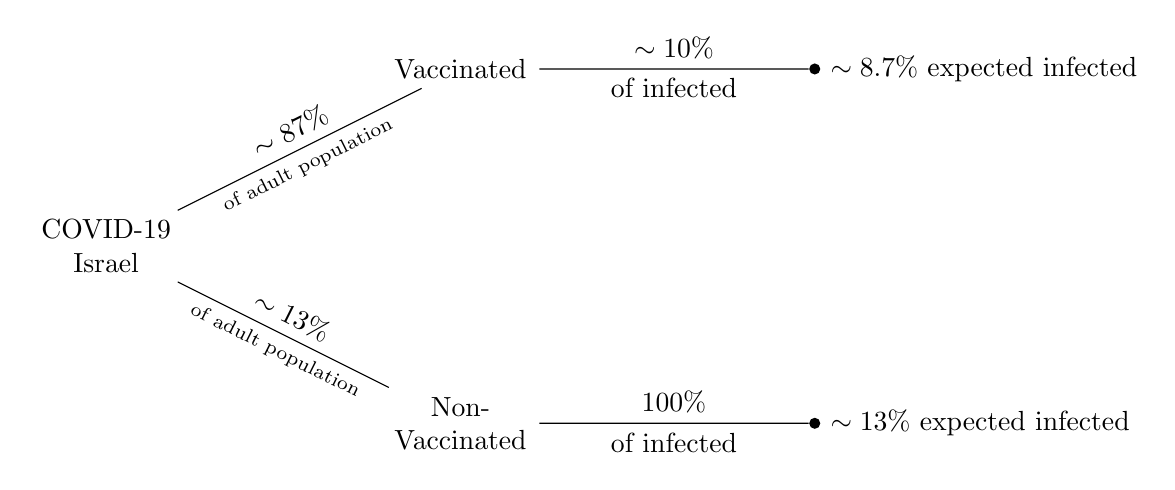
\begin{tikzpicture}[grow=right, sloped]
	\centering
	\node[bag] {COVID-19 Israel}
	    child {
	        node[bag] {Non-Vaccinated}        
	            child {
	                node[end, label=right:
	                    {$\sim 13\%$ expected infected}] {}
	                edge from parent
	                node[above] {$100\%$}
	                node[below]  {of infected}
	            }
	            edge from parent 
            node[above] {$\sim 13\%$}
            node[below]  {{\scriptsize of adult population}}
	    }
	    child {
	        node[bag] {Vaccinated}        
	        child {
	                node[end, label=right:
	                    {$\sim  8.7\%$ expected infected}] {}
	                edge from parent
	                node[above] {$\sim  10\%$}
	                node[below]  {of infected}
	            }
	            edge from parent 
            node[above] {$\sim  87\%$}
            node[below]  {{\scriptsize of adult population}}
	    };
	\end{tikzpicture}
	
	\end{figure}
	So as proven thanks to the decision tree above, $40\%$ is exactly what is expected and is a very good result. So adding the word \og despite \fg{} was a double mistake!!! Notice that one week after the title of the article still wasn't corrected by the redaction team of CNews...
	
	Notice that a minority of people don't understand - because of a lack of Statistical education or just because of a difficulty to apprehend the concept of proportions - why when a huge majority of people are vaccinated then the majority of people who are sick will be... vaccinated people. For example if you take the extreme case where $100\%$ of the population is vaccinated than obviously you will have at the emergencies $100\%$ of vaccinated people... But in absolute value that will still be less people than if no one was vaccinated.
	
	Let us denote as always the efficiency of a vaccine by it's Odds Ratio O.R. (\SeeChapter{see section Numerical Methods page \pageref{odds ratio confidence interval}}). Then $1-\text{O.R.}$ is obviously its ineffectiveness. Denoting by HR the hospitalisation rate of people who catches the illness, $P_\text{V}$ the population of vaccinated people and $P_\text{NV}$ the population of non-vaccinated people then the number of hospitalized are respectively for each population:
	
	Equating to get the threshold of ratio of population at which the number of hospitalized vaccinated people is equal to that of non-vaccinated we get immediately after rearranging:
	
	So for example with a vaccine having an efficiency of $\text{O.R.}=95\%$. We will get the same number of hospitalized vaccinated and non-vaccinated people when the ratio in the whole population is of $1/(1-95\%)=20$ vaccinated for $1$ vaccinated. If we want to transform this value into a whole population limit ratio (WPLR) then we just calculate:
	
	Applying this to our example we get:
	
	That means we reach an equality of hospitalized vaccinated and non-vaccinated people when $95.238\%$ of the whole population is vaccinated for a vaccine with $95\%$ efficiency.
	
	Such a poor comprehension of proportions by some uneducated people can be well illustrated by the following figure:
	\begin{figure}[H]
		\centering
		\includegraphics[width=0.8\textwidth]{img/economy/covid_proportions.jpg}
	\end{figure}
	
	\begin{tcolorbox}[title=Remark,colframe=black,arc=10pt]
	As always, there exist much more elaborated models like for example the SEIR model Susceptible - Exposed - Infectious - Recovered - Susceptible). In this category of models, individuals experience a long incubation duration (the "exposed" category), such that the individual is infected but not yet infectious! There is also SEIRS (Susceptible - Exposed - Infectious - Recovered - Susceptible) model, where recovered people may become susceptible again (recovery does not confer lifelong immunity). But also the SIRD model Susceptible-Infectious-Recovered-Deceased, the SIRV model Susceptible-Infectious-Recovered-Vaccinated model, the MSIR model Measles-Infectious-Recovered, etc. For more see \cite{hethcote2000mathematics}.
	\end{tcolorbox}
	
	\paragraph{Incidence rate}\mbox{}\\\\
	In epidemiology, "\NewTerm{incidence}\index{incidence}\label{incidence}" is a measure of the probability of occurrence of a given medical condition in a population within a specified period of time. Although sometimes loosely expressed and understood - that's why we treat it shortly here - simply as the number of new cases during some time period, it is better expressed as a proportion or a rate with a denominator.
	
	The numerical portion of an incidence rate has a lower bound of zero but has no upper bound; it has the mathematical range for the ratio of two non-negative quantities, in this case the number of events in the numerator and the person-time in the denominator. 
	
	At first, it may seem surprising that an incidence rate can exceed the value of $1.0$, which would seem to indicate that more than $100 \%$ of a population is affected. It is true that at most, only $100 \%$ of persons in a population can get a disease, but the incidence rate does not measure the proportion of a population with illness and in fact is not a proportion at all.
	
	Recall that incidence rate is measured in units of the reciprocal of time. Among $100$ people, no more than $100$ deaths can occur, but those 100 deaths can occur in $10,000$ person-years, in $1,000$ person-years, in 100 person-years, or even in $1$ person-year (if the $100$ deaths occur after an average of $3.65$ days each). 
	
	An incidence rate of $100$ cases (or deaths) per $1$ person-year might be expressed as:
	$$100\; [\text{cases}\cdot\text{person-year}^{-1}]$$
	It might also be expressed as:
	$$10,000\;[\text{cases}\cdot\text{person-century}^{-1}]$$
	or ($100/12=8.\bar{3}$):
	$$8.\bar{3}\;[\text{cases}\cdot\text{person-month}^{-1}]$$ 
	or ($100/52\cong 1.92$):
	$$1.92\; [\text{cases}\cdot\text{person-week}^{-1}]$$ 
	or ($100/365\cong 0.27$):
	$$0.27\;[\text{cases}\cdot\text{person-day}^{-1}]$$
	The numerical value of an incidence rate in itself has no interpretability because it depends on the arbitrary selection of the time unit! It is thus essential in presenting incidence rates to give the appropriate time units, either as in the examples given above or as in $8.33\;[\text{month}^{-1}]$ or $1.92\;[\text{week}^{-1}]$. Although the measure of time in the denominator of an incidence rate is often taken in terms of years, one can have units of years in the denominator regardless of whether the observations were collected over $1$ year of time, over $2$ week of time, or over $10$ years of time.

	Unfortunately, the interpretation of incidence rates as the inverse of the average "waiting time" will usually not be valid unless the incidence rate is calculated for a stationary population with no migration (no immigration or emigration) or a closed population with complete follow-up. For example, the death rate for the United States in 1977 was $0.0088$ year $^{-1} ;$ in a steady state, this rate would correspond to a mean life span, or expectation of life, of 114 years. Other analyses, however, indicate that the actual expectation of life in 1977 was $73$ years. The discrepancy is due to immigration and to the lack of a steady state. Note that the no-migration assumption cannot hold within specific age groups, for people are always "migrating" in and out of age groups as they age.

	\begin{tcolorbox}[title=Remark,colframe=black,arc=10pt]
	Incidence should not be confused with "\NewTerm{prevalence}\index{prevalence}\label{prevalence}", which is the proportion of cases in the population at a given time rather than rate of occurrence of new cases. Thus, incidence conveys information about the risk of contracting the disease, whereas prevalence indicates how widespread a disease is.
	\end{tcolorbox}
	
	\pagebreak
	\subsubsection{Lotka–Volterra predator–prey model}\label{lotka volterra model}
	This predator-prey interaction model was proposed by Volterra after the First World War. The purpose was to explain the dynamics of populations of sardines and sharks in the Adriatic (and hop! a bit of Oceanography in this book...!). Especially to explain in why the quantities of sardines fished after the interruption due to the war were not as important as before (which may seem counter-intuitive) and why at the resumption of fishing the observed proportion of sharks increased.
	
	Taking again what we saw at the beginning of this section by writing $N(t)$ the number of preys and $P(t)$ the number of predators (that is to say implicitly a growth following a power law of the number of preys, in absence of fishing):
	
	
	and in the absence of preys (in the case of fishing), the number of predators decrease also following a power law, we have respectively:
	
	At this point of the speech, we must consider two species (preys and predators) that are obviously not isolated but in interaction. To quantify the contribution of the interaction between species, we will consider only predation, by assuming that is value or intensity (of interaction) is a function of the probability of prey-predators to meet together that will be supposed proportional to the product $N\cdot P$ of the percentages of the two populations.
	
	These meetings do not have the same effects on both species. First, of course, each prey eaten by a predator is a net gain for the population of the latter and a net loss for the first. Thus, if the effect of interactions is accepted as being proportional to $N\cdot P$, the signs of the influence of interaction differ for the two species so that our equations with interaction this time become:
	
	This system of equation is named the "\NewTerm{Lotka-Volterra model}\index{Lotka-Volterra model}".
	
	Before going further, let us seek for the values for which the derivatives vanish (which will give us in fact the equilibrium point of the system):
	
	where $N'$ and $P'$ are the values that cancel the derivatives (not to be confused this time with the notation sometimes used to condense the writing of a derivative !!!).
	
	Thus:
	
	A trivial solution is the "\NewTerm{extinction solution}" (also sometimes named "{critical solution}") given by:
	
	Otherwise, we also have as a possible solution:
	
	Now we normalize these equations by writing (so they are dimensionless):
	
	with this normalization, the model can be rewritten:
	
	By rearranging the coefficients, the system can finally be written (excluding the solution of inexistence, ie non-existence):
	
	for which derivatives vanish at the point $(1,1)$.
	
	The discreet plot of this system of equations (in which we recognize a logistic term as seen in the section of Populations Dynamics) gives us with $m=r=b=c=1$ and initial conditions $(x_0,y_0)=(4,1)$:
	\begin{figure}[H]
		\centering
		\includegraphics{img/economy/cycle_offer_demand.jpg}
		\caption{Theoretical fluctuation of population}
	\end{figure}
	In comparison here is a practical (real) example of prey-predators measurements (Hares-Lynx) by the Hudson Bay-Company (when we seek for data corresponding to a model we will finish soon or late to find data fitting the model...):
	\begin{figure}[H]
		\centering
		\includegraphics{img/economy/lotka_volterra_offer_demand_hudson.jpg}
		\caption[]{Hudson Bay-Company real Lotka-Volterra measurements}
	\end{figure}
	The two previous figures represent the variables $x$ and $y$ as a function of time. However, what can be interesting for a scientist (or an economist) is the representation of $y$ in terms of $x$ and vice versa. Thus, we obtain for the same initial conditions $m, r, b, c$ and for the various initial values of $(x_0,y_0)$ (the Predators is in ordinate and the Preys on the abscissa):
	\begin{figure}[H]
		\centering
		\includegraphics{img/economy/offer_demand_space_phase.jpg}
		\caption{Representation in phase space prey/predator cycle}
	\end{figure}
	The above figure is very interesting to interpret when you follow a path in the counter-clockwise direction.
	
	Thus we see (in the phase space representation) that for fixed initial conditions, the system is periodic and has trivially an equilibrium point at:
	
	named "\NewTerm{fixed points}" that correspond to the points where:
	
	Finally, we have two pairs of equilibrium points (that is almost trivial, looking at the system of equations):
	
	The question that will naturally arise is the "real" direction of rotation (representation) of the phase plane. Thus, representing the directions using a vector field, we get the representation which is effectively counter-clockwise (more interesting representation to understand what happened after 1st World War):
	\begin{figure}[H]
		\centering
		\includegraphics{img/economy/offer_demand_vector_field.jpg}
		\caption{Rotation direction offer/demand phase space}
	\end{figure}
	
	To know in which direction we are going in the phase space at a given time, it suffices to know the derivative $\mathrm{d}y /\mathrm{d}x$ (or vice versa $\mathrm{d}x /\mathrm{d}y$). Therefore we have:
	
	That said, we see well on the phase diagram with vector field as vectors that it comes a time in the cycle of this model where the offer is very high for low demand. So the mathematical model (theoretical) clearly explains what can be a priori counter-intuitive to many humans (offer creates the demands).
	
	However, we can (must) ask ourselves the question of what happens after a small perturbation around the equilibrium point.
	
	So we have the following Lotka-Volterra system in equilibrium:
	
	By putting an infinitely small perturbation, it is will be written:
	
	Neglecting the quadratic $xy$ terms, we obtain:
	
	\begin{enumerate}
	\item We focus first on the study near the point of extinction $(0,0)$, this is why we can neglect the quadratic terms $xy$ but the expression remain too complicated. So, always considering we are near the point of extinction $(0,0)$, we consider a bit unfairly but cleverly (otherwise we still could not solve the problem analytically) the following approximations:
	
	Therefore:
	
	This shows us for the system in equilibrium, close to the inexistence point, the prays decreases exponentially (power law) as predators increases exponentially:
	
	This shows us for the equilibrium system, near the extinction point, that the number of individuals predators decreases exponentially while the prey are increasing exponentially. This has a biological sense: when there are few individuals predators, then prey multiply and at the same time the number of prey increases, predators multiply and concentrate increasingly on their prey; respectively when there are few prey only, the number of predator decreases as the number of prey increases (ahhh nature...).
	
	\begin{tcolorbox}[title=Remark,colframe=black,arc=10pt]
	In the literature we find sometimes the "-" sign in the top or bottom in the previous equations. In reality, the position of the "-" sign is not important because it is just the starting choice in the system dynamics.
	\end{tcolorbox}
	
	\item Close to the equilibrium point $(1,1)$ we start from:
			
		And we put $x:=1+x,y:=1+y$ where $x,y$ are now small perturbations near the point $(1,1)$. Therefore we have:
		
		 (hop! we change the position of the "-" sign on purpose to show that this is only a starting choice !!!):
		
		To solve this system, let us differentiate the first equation once again:
		
		and by injecting in it $\mathrm{d}y/\mathrm{d}t$:
		
		So we get a small second order differential equation (\SeeChapter{see section Differential and Integral Calculus page \pageref{second order differential equations}}). Whose typical simple solution is:
		
		By injecting this solution into the differential equation, we obtain after simplification of exponentials a simple polynomial of the second degree (\SeeChapter{see section Calculus page \pageref{polynomial}}):
		
		Whose solution is trivial:
		
		Thus, the general solution of the differential equation is the linear combination of the two special solutions we get:
		
		But we therefore have:
		
		Therefore, knowing $x(t)$ we obtain easily:
		
		Now let us use the Euler formula (\SeeChapter{see section Numbers page \pageref{euler formula}}):
		
		Thus we have:
		
		and as (\SeeChapter{see section Trigonometry page \pageref{remarkable angles}}) $\cos(x)=\cos(-x),-\sin(x)=\sin(-x)$ then we have:
		
		and similarly, we obtain:
		
		Thus, around the equilibrium point $(1,1)$ with sufficiently small perturbations to validate linearisation the system oscillate as ellipses (or circles) whose axes are defined by the two equations above.
	\end{enumerate}
	We can get the graphs above with Maple 4.00b (this is a nice example of application of this software):
	
	\texttt{>restart: with(plots): with(DEtools):}\\
 	\texttt{>rate\_eqn1:= diff(h(t),t)=(0.1)*h-(0.005)*h*(1/60)*u;}\\
 	\texttt{rate\_eqn2:=diff(u(t),t)=(0.00004)*h*u-(0.04)*u;vars:= [h(t), u(t)];}\\
 	\texttt{>init1:=[h(0)=2000,u(0)=600]; init2:=[h(0)=2000,u(0)=1200]; init3:=[h(0)=2000, u(0)=3000];domain := 0 .. 320;}\\
 	\texttt{>L:= DEplot({rate\_eqn1, rate\_eqn2}, vars, domain,{init1}, stepsize=0.5, scene=[t, u], arrows=NONE):}\\
  	\texttt{>H:= DEplot({rate\_eqn1, rate\_eqn2}, vars, domain,{init1 }, stepsize=0.5, scene=[t, h], arrows=NONE):}\\
  	
  	\begin{figure}[H]
		\centering
		\includegraphics{img/economy/lotka_volterra_offer_demand_maple.jpg}
		\caption{Lotka-Volterra offer/demand model periodic plot in Maple 4.00b}
	\end{figure}
  	
  	\texttt{>DEplot({rate\_eqn1, rate\_eqn2}, vars, t= 0 .. 160, {init1, init2, init3}, stepsize=0.5, scene=[h,u], title='Demand vs. 60 * Offer for t = 0 .. 160', arrows=slim);}\\
  	
  	\begin{figure}[H]
		\centering
		\includegraphics{img/economy/lotka_volterra_offer_demand_phase_space_maple.jpg}
		\caption{Lotka-Volterra offer/demand phase space model plot in Maple 4.00b}
	\end{figure}
	
	\pagebreak
	\subsection{Schaefer's Optimal capture model}
	A useful principle for the management of fishing, hunting, wild collection quotas or exploitation of raw materials is the "\NewTerm{maximum sustainable yield}" which is directly linked to the good management of the exploited dynamics of the concerned population.
	
	\textbf{Definition (\#\mydef):} The "\NewTerm{maximum sustainable yield}" is the maximum amount of fish, deer, birds or fungi, etc. which can be killed / harvested in a population without jeopardizing its survival.
	
	Determine this maximum sustainable yield give the possibility the get to the goal of fishing, hunting, gathering as much as possible, without falling into the overconsumption that potentially lead to the disappearance of the population.
	
	The distinction between a balanced consumption of natural resources and an exaggerated one is often hard to do. Mathematical and statistical models are then always useful and necessary to establish that frontier.
	
	The calculations are involved in the calculations of quotas even still in the early 21st century. The simplistic model that we will present is used by some large States (but it will in time disappear to make way for a more sophisticated model with probabilistic parameters).
	
	We are therefore interested in the biomass of a population of a consumable. The model put forward by Schaefer in 1954 involves only two parameters:
	\begin{enumerate}
		\item The maximum biomass $M$ that can live constantly in a system

		\item The reproduction rate $r$
	\end{enumerate}
	We start from the assumption (to check in practice because of the Lotka-Volterra model) that at the year zero (before to the consumption of the resource), the corresponding biomass is:
	
	The empirical model is:
	
	To understand this model, let assume first that the population is not exploited, that is to say that $C=0$. At the  year $n$, the population then increases of:
	
	Thus, in the absence of fishing, if $X_0$ is smaller than $M$, the population will grow slowly until it reaches its maximum capacity $M$.
	
	In the extreme case, where consumption $C$ is equal to $M$, we have:
	
	which makes sense ... (there is a total extinction!).
	
	Now rewrite the Schaefer model as follows:
	
	We would like to know for what value of $X_n$, we would have the biomass which no longer varies. That is to say:
	
	Therefore:
	
	So it is a simple equation of the second degree! It has a real solution only if the discriminant (\SeeChapter{see section Calculus page \pageref{discriminant}}) is positive or zero. Therefore, knowing that $r$ is positive or zero by construction:
	
	Thus, the maximum possible value of $C$ is $rM/4$. When we replace $C$ by this value in the original equation:
	
	we get:
	
	Therefore:
	
	Therefore the solution is:
	
	Thus, there exists a time $n$ (infinite) for which the population tends asymptotically to $M/2$ at the condition that $X_0\geq \dfrac{M}{2}$.
	
	Still its simplicity and its deterministic aspect  the Schaefer model is still used in the early 21st century in fisheries management.
	
	\subsection{Hardy-Weinberg model}
	The Hardy-Weinberg model (developed in 1908) describes the diversity (rather than evolution) of living in the point of view of population genetics. However, this model still allows to understand the impact of a mutation agent on a population of individuals and therefore to solve problems related to the refusal of the Natural selection model  (evolution) of Darwin. Indeed, Darwin's work focused on characters that varied continuously. But he could not explain how individuals transmit these changes (this is actually quite annoying). The Mendel's genetics, meanwhile imposed that only discontinuous traits were hereditary.
	
	So there was  a conflict between the continuous model (Darwin) and  the discontinuous one (Mendel) and it was genetics that in the twentieth century helped to establish that fact that it is the mix of genes that creates diversity and verbatim natural selection.
	
	\begin{tcolorbox}[title=Remark,colframe=black,arc=10pt]
	We will prove in the section of Numerical Methods (chapter of Theoretical Computing) as part of the study of genetic algorithms that the chromosome having the biggest function value of "fitness" will be the one most likely to reproduce. This is part of the theorem named "The Schema Theorem" ...
	\end{tcolorbox}
	
	Conclusion: The evolution is not made at the level of the individual but of the population (this is a quite good lesson to remember...)
	\begin{enumerate}
		\item[D1.] A gene or "\NewTerm{genotype}\index{genotype}\label{genotype}" is composed of "\NewTerm{alleles}\index{alleles}" (usually $2$, so we will consider individuals as being "$diploid$")
		
		So the genotype is the genetic makeup of an organism. It's basically which alleles an organism has for a specific gene or trait. This is what causes genetic variations.

		\item[D2.] A "\NewTerm{gene pool}\index{gene pool}" is a set of genes present in a population.

		\item[D3.] A "\NewTerm{micro-evolution}\index{micro-evolution}" is a change in the frequency of alleles of a gene pool of a population.

		\item[D4.] An allele is named "\NewTerm{fixed allele}" when all members of a population have two identical alleles. 

		\item[D5.] A "\NewTerm{speciation}\index{speciation}" is a long-term occurrence of a micro-evolution, making appear a new species.

		\item[D6.] The "\NewTerm{mutation}\index{mutation}" is an evolutionary agent that alters the gene pool of a population by producing new genes (we therefore consider that there is no evolutionary agents at work in the population in this model).
	\end{enumerate}
	
	\begin{tcolorbox}[title=Remark,colframe=black,arc=10pt]
	Mutation is a rare event and usually harmful. Its quantitative effects are greater in short generation time organisms (bacteria and viruses), the effect is much less pronounced among organisms with long generation time (animals and plants).
	\end{tcolorbox}
	
	\begin{figure}[H]
		\centering
		\includegraphics[scale=0.6]{img/economy/genotype_vs_phenotype.jpg}
		\caption[Genotype vs Phenotype]{Genotype vs Phenotype (source: TESL.com)}
	\end{figure}
	
	Let us now consider a population consisting of $13$ individuals (1 gene, each consisting of two alleles selected among 3):
	
	Therefore we have the following relative allele frequencies:
	
	with obviously:
	
	And the following relative genotype frequencies:
	
	with obviously:
	
	To summarize, if we now consider a population of individuals possessing genes made of only two types of alleles, we have therefore (more concrete case relatively to the actual living biology on Earth):
	
	So we have for the relative frequency of the number of alleles $B$:
	
	and for the relative frequency of allele $b$:
	
	With obviously:
	
	This can be illustrated (by changing the letter $B$ by $Y$ and $b$ by $y$):
	\begin{figure}[H]
		\centering
		\includegraphics[scale=0.6]{img/economy/monohybrid_cross.jpg}
		\caption[Monohybrid cross]{Monohybrid cross (source: OpenStax)}
	\end{figure}
	We can see in the figure above that the allele relative frequencies are $50\%/50\%$, the genotype relative frequencies are $25\%,50\%,25\%$ (also often denoted $1:2:1$) and the phenotype relative frequency $66.\bar{6}\%,33.\bar{3}\%$ (also often denoted $3:1$).
	
	We can make a few observations about the way of constructing this model. Indeed, the frequency of alleles (genetic equilibrium) remains in a population approximately constant generation after generation if:
	\begin{enumerate}
		\item The population is very large (a tiny disturbance changes only a little bit the frequency of the types of genotypes).

		\item No emigration or immigration (no new types of alleles in the population).

		\item No mutations altering the alleles (this contains the point number 2).

		\item Random couplings (not influenced by the type of allele studied).

		\item No natural selection (this contains the point number 4).
	\end{enumerate}
	It may be relevant (for general knowledge) to highlight the fact that we distinguish two types of non-random accouplement:
	\begin{enumerate}
		\item Inbreeding: crossing between individuals of the neighbourhood, thus having family links; in species dispersing only a little bit. This apply especially to vegetables.

		\item Homogamy: free choose of partners who have some similarities for given physical characters. This apply especially among animals.
	\end{enumerate}
	The inbreeding and homogamy accouplement is not a direct cause of micro-evolution since they do not alter the gene pool of a population. However, if some individuals coming from this non-random accouplement are more likely to have accouplement with others (natural selection), it will follow a change in the allele frequency in the downward population and therefore a micro-evolution. As a result, non-random accouplement are a potential factor of micro-evolution.
	
	Finally, to return to our model, the probability that an individual has one of three possible genotypes (relatively to a genotype) in the population (relative to our example) is:
	\begin{enumerate}
		\item Probability that an individual is $BB$:
		

		\item Probability that an individual is $bb$:
		

		\item Probability that an individual is $Bb$ or $bB$:
		
	\end{enumerate}
	Finally, we get the "\NewTerm{Hardy-Weinberg equation}\index{Hardy-Weinberg equation}" (for the special case of two alleles):
	
	That we can represent the graph:
	\begin{figure}[H]
		\centering
		\includegraphics{img/economy/hardy_weinberg.jpg}
		\caption[Plot of the Hardy-Weinberg equation]{Plot of the Hardy-Weinberg equation (author: Antonín Šípek)}
	\end{figure}
	A population that is not changing genetically is in Hardy-Weinberg equilibrium if these five assumptions are correct:
	\begin{itemize}
		\item Random mating (panmixia)
		\item Large population size ($N$ approaching infinity)
		\item No migration between populations
		\item No (or negligible) mutations
		\item Natural selection does not affect alleles being considered
	\end{itemize}
	If these assumptions are true, it follows that:
	\begin{itemize}
		\item Allele frequencies remain constant from one generation to the next
		\item After one (or more) generations of random mating (breeding), the genotype frequencies (for a $2$-allele gene with allele frequencies $p, q$) are in the proportions: $p^2_{(AA)} : 2pq_{(Aa)} : q^2_{(aa)}$, and population will be in H-W equilibrium.
		\item For a population to be in Hardy Weinberg equilibrium, the observed genotype frequencies must match those predicted by the equation $p^2 + 2pq + q^2$.
	\end{itemize}
	
	The Hardy–Weinberg principle may also be generalized to polyploid\footnote{Humans are called "diploid organisms" because they have two alleles at each genetic locus, with one allele inherited from each parent.} systems, that is, for organisms that have more than two copies of each chromosome. Consider again only two alleles. Multinomial expansion for two alleles $A$ and $a$ with frequencies $p$ and $q p^{2}+2 p q+q^{2}$ is a binomial expansion of $(p+q)^{2}$. That is:
	
	For three alleles $A$, $B$ and $C$ with frequencies $p, q$ and $r$, the multinomial expansion is $(p+q+r)^{2}$ which expands into:
	
	where the first three terms being homozygotes and the remaining three heterozygotes. Therefore the three alleles Hardy-Weinberg equation is given by:
	
	\begin{figure}[H]
		\centering
		\includegraphics[scale=0.4]{img/economy/punnett_square_three_alleles.jpg}
		\caption[Punnett square for three-allele case]{Punnett square for three-allele case (source: Wikipedia)}
	\end{figure}
	
	therefore the polyploid case is the polynomial expansion of $(p+q)^{c}$,
where $c$ is the ploidy, for example with tetraploid ($c = 4$):
	\begin{table}[H]
		\centering
		\begin{tabular}{|l|l|}
		\hline Genotype & Frequency \\
		\hline $AAAA$ & $p^{4}$ \\
		\hline $AAAa$ & $4 p^{3} q$ \\
		\hline $AAaa$ & $6 p^{2} q^{2}$ \\
		\hline $Aaaa$ & $4 p q^{3}$ \\
		\hline $aaaa$ & $q^{4}$ \\
		\hline
		\end{tabular}
	\end{table}
	For $n$ distinct alleles in $c$-ploids, the genotype frequencies in the Hardy-Weinberg equilibrium are given by individual terms in the multinomial expansion of $\left(p_{1}+\cdots+p_{n}\right)^{c}$ :
	
	After this study, we can finally (re)defined the "\NewTerm{Darwin's law}\index{Darwin's law}" so it give us the possibility to eliminate the problem of the big question (problem) of continuous or discrete changes:
	
	\textbf{Definition (\#\mydef):} Natural selection is an evolutionary agent that alters the gene pool of a population by increasing the frequency of alleles producing phenotypes\label{phenotype} (genotypes defines the behaviour of an individual) best suited to the medium (environment). Thus, the individuals that are the best adapted to their environment reproduce more than others and contribute more to the genetic heritage of the descendants. The frequency of good genes gradually increases in the population from generation to generation. Thus, natural selection directs the adaptation of a population to its environment by accumulating genotypes that promote survival in the medium (environment).
	
	A study \cite{nachman2000estimate} provides some evidence that average mutation rate can be estimated to approximately $175$ mutations per diploid genome per generation ($\sim 2.5\cdot 10^{-8}$ per base per generation). The highest per base pair per generation mutation rates are found in viruses \cite{drake1998rates}, which can have either RNA or DNA genomes. DNA viruses have mutation rates between $10^{-6}$ to $10^{-8}$ mutations per base per generation, and RNA viruses (whose genomes contain ca. $10^{4}$ bases) have mutation rates between $10^{-3}$ to $10^{-5}$ per base per generation.
	
	 The high-resolution figure below (you can deeply zoom in for the details!) represents a robust evolutionary timescale for all approximately 6,000 living species of mammals \cite{upham2019inferring}:
	\begin{figure}[H]
		\centering
		\includegraphics[width=0.93\textwidth]{img/economy/philogenetic_tree.pdf}
		\caption{Species-level relationships and tempo of diversification across mammals}
	\end{figure}
	
	\begin{tcolorbox}[title=Remarks,colframe=black,arc=10pt]
	\textbf{R1.} The Hardy-Weinberg model is very unlikely in nature. Indeed, the probabilities that all the necessary assumptions are present simultaneously is quite low. However, this is a theoretical model that evaluates if there is a micro-evolution in a population. Thus, we measure the frequency of alleles in the parent population and then we apply the Hardy-Weinberg equation. If the genetic structure of the descendant population differs from that predicted by the law, then we know that at least one agent of evolution is at work.\\
	
	\textbf{R2.} This theoretical model can help to predict a punctual estimator of the social costs of genetic diseases. Indeed, if we know the percentage of individuals with recessive disease in a population, we can apply the Hardy-Weinberg equation and evaluate the number of healthy transmitters and then we can predict the likelihood of the disease in future generations. If it is large (this reasoning is valid only in a liberal and capitalist framework), we may decide to invest in research or providing funds to treat the sick people.\\
	
	\textbf{R3.} For people interested in exploring the subject further, we highly recommend reading \cite{crow2009introduction} and \cite{hamilton2011population}, which are two masterpiece in this field!
	\end{tcolorbox}	
	\begin{tcolorbox}[colframe=black,colback=white,sharp corners]
	\textbf{{\Large \ding{45}}Examples:}\\\\
	E1. Given a genotype of possible sequences $\{BB,bb,Bb\}$ and let consider that $p_B=0.6,p_b=0.4$. We then have:
	
	Therefore, in a population of $1'000'000$ individuals, we should have:
	

	E2. If in Quebec ($6$ million inhabitant), one in five has blue eyes ($bb\Rightarrow q^2=1/5$), how many people are of genotype $BB$ and how many of type $Bb$?
	
	Therefore:
	
	Therefore we have:
	
	
	E3. We introduce $1,000$ spotted frogs in a pond (homozygous for this characteristic: $TT$) and $250$ frogs without spots (homozygous for this trait: $tt$). If we allow the frogs to reproduce for several years, assuming that the population remains stable, what number of frogs $TT, Tt, tt$ should we then observe?\\
	
	So we have a population of $1,250$ individuals in which we $1,000 TT$ ($2,000$ allele $T$) and $250 tt$ ($500$ alleles $t$). So:
	
	If the population is of $1,250$ people, we have:
	
	\end{tcolorbox}


	\subsection{Mendel's law}
	During methodical hybridization of many species and varieties of various plants, it has been observed, in general, the uniformity and character of the first hybrid generation ($G1$) intermediate between the parents. So the inheritance is totally taken form the dominant character in the first generation (father or mother but of the mix). At the second generation ($G2$) occurs polymorphism showing various combinations of characters of the initial generation ($G0$). Thus we find in the second generation $25\%$ of individuals with non-dominant character of the initial generation and $75\%$ with the dominant character. The character that was masked in,the first generation (G1) is then named "\NewTerm{recessive character}".
	
	This fact can be summarized with the following structure:
	\begin{figure}[H]
		\centering
		\includegraphics[scale=0.75]{img/economy/mendel.jpg}
	\end{figure}
	Mendel then made the assumption that the gametes of hybrids of the first generation ($G1$) must be in equal numerical proportions, of the type of one or other of the parents. This is the "\NewTerm{law of purity of gametes}".
	
	It has been established that human blood groups also obey to the rules of Mendelian inheritance. Thus, $A$ and $B$ blood groups are dominant and can appear in children if and only if they are present by the parents.
	
	In a more pedagogical way, the previous figure can be illustrated as following:
	\begin{figure}[H]
		\centering
		\includegraphics[scale=0.75]{img/economy/mendel_more_illustrative.jpg}
	\end{figure}
	
	Mendel's laws are stated as following:
	\begin{itemize}
		\item[L1.] "\NewTerm{Law of dominance and uniformity}": Some alleles are dominant while others are recessive; an organism with at least one dominant allele will display the effect of the dominant allele.
	
		\item[L2.] "\NewTerm{Law of segregation}": During gamete formation, the alleles for each gene segregate from each other so that each gamete carries only one allele for each gene.
	
		\item[L3.] "\NewTerm{Law of independent assortment}": Genes of different traits can segregate independently during the formation of gametes.
	\end{itemize}
	
	\begin{tcolorbox}[title=Remark,colframe=black,arc=10pt]
	After Mendel's studies and discoveries more and more new discoveries about genetics were made. Mendel himself has said that the regularities he discovered apply only to the organisms and characteristics he consciously chose for his experiments. Mendel explained inheritance in terms of discrete factors- genes - that are passed along from generation to generation according to the rules of probability. Mendel's laws are valid for all sexually reproducing organisms, including garden peas and human beings. However, Mendel's laws stop short of explaining some patterns of genetic inheritance. For most sexually reproducing organisms, cases where Mendel's laws can strictly account for all patterns of inheritance are relatively rare. Often the inheritance patterns are more complex.\\

	In cases of codominance the phenotypes produced by both alleles are clearly expressed. Mendel chose genetic traits in plants that are determined by only two alleles, such as "$A$" and "$a$". In nature, genes often exist in several different forms with multiple alleles. Furthermore, many traits are produced by the interaction of several genes. Traits controlled by two or more genes are said to be polygenic traits.
	\end{tcolorbox}
	
	\pagebreak
	\subsection{Growth rate with temperature}
	For many species (mammals, fish, micro-organisms), it is reasonable to consider as a first approximation, the relation of the population growth rate with the temperature of the environment is a second degree polynomial:
	
	where the values $a,b,c$ will depend of the considered species.
	
	We know also that there is for most individuals a given optimum growth rate at a given temperature denoted $T_{\text{opt}}$, as well as minimum $T_{\min}$ and maximum $T_{\max}$ temperatures below and above which there is no more growth.

	Therefore, the parameters $a, b, c$ must satisfy the following relations:
	
	This implies for the three temperatures $T_{\text{opt}}, T_{\min}, T_{\max}$ to respect the relations proved in the context of the study of polynomials of the second degree in the section Calculus:
	
	So if we know for a living entity $T_{\text{opt}}$ and $T_{\min}$ it is easy to deduce theoretically an approximation of $T_{\max}$ in the context of the main assumption...
	
	\begin{tcolorbox}[title=Remark,colframe=black,arc=10pt]
	Again, for people interested in exploring the subject further, we highly recommend reading \cite{crow2009introduction}, which is a masterpiece in this field!
	\end{tcolorbox}	
	
	\begin{flushright}
	\begin{tabular}{l c}
	\circled{90} & \pbox{20cm}{\score{2}{5} \\ {\tiny 57 votes,  60.00\%}} 
	\end{tabular} 
	\end{flushright}
	
	%to make section start on odd page
	\newpage
	\thispagestyle{empty}
	\mbox{}
	\section{Game and Decision Theory}\label{game and decision theory}
	\lettrine[lines=4]{\color{BrickRed}T}he decision and game  theory goes far beyond the narrow confines of social games, even if they constituted the first object of study and gave it its name in most commercially available books. Furthermore, the two theories are very close to each other from which the fact that they are very often non-differentiated in the literature.
	
	\textbf{Definitions (\#\mydef):} 
	
	\begin{enumerate}
		\item[D1.] The "\NewTerm{Game theory}\index{game theory}" is the study of decision making models in uncertain future with unknown probabilities.
		
		\item[D2.] The "\NewTerm{Decision theory}\index{decision theory}" (sometimes also called "decision analysis") is the study of decision-making models in an uncertain probabilistic (objectively or subjectively) future.
		
		\item[D3.] The "\NewTerm{Data drive decision making}" is the practice of basing decisions on the analysis of data ("\NewTerm{Machine Learning"} or "\NewTerm{Data Mining"}), rather than purely on intuition (\SeeChapter{see section Numerical Methods page \pageref{data mining}}).
	\end{enumerate}
	Each of the methods of analysis of these two theories is mainly made in tabular (table) form or as a vertical or horizontal tree.
	
	Here is a fairly familiar pattern for project manager who sums up the whole situation (data driven decision is not included as treated in the Theoretical Computing section during the study of decision trees):
	\begin{figure}[H]
	\centering
	\includegraphics[scale=0.75]{img/economy/decision_classification_techniques.eps}
	\caption{Elementary classification of decision techniques}
	\end{figure}
	These tools aim to try to formalize to decide which configuration or decision is better than another? We will look for this purpose to find the optimum of certain parameters that quantify the quality of a strategic situation. We must also determine which conditions lead to a configuration that is considered optimal.

	Game theory and the decision is now quite common and used in academic circles, not only in economy (particularly corporate finance), but also by a whole class of other science in which the study on conflictual situations is relevant: sociology, biology, evolution, computer (video games), marketing, etc.

	\begin{tcolorbox}[title=Remark,colframe=black,arc=10pt]
In the world of corporations, and especially in Europe, decisions techniques are unknown to almost all of the leaders whose choices are often more qualitative and instinctive than scientific and thus less accurate...
	\end{tcolorbox}	
	
	We will try, as always in this book, to minimize as possible the number of definitions and concepts in order not to drown the rigour of mathematical analysis in the chaos of useless vocabulary and not necessary for such analysis (and in the field of game theory it is otherwise a bit like in graph theory... a real nightmare of definitions!).

	\textbf{Definition (naive \#\mydef):} A "\NewTerm{game}\index{game}" is a situation where the players are driven to make strategic choices among a number of possible actions, within the framework defined in advance by the "\NewTerm{rules of the game}", the result of these choices constituting an "\NewTerm{outcome of the game}", which is associated with a "\NewTerm{gain}" (or payment), positive or negative, for each player.

	\begin{tcolorbox}[title=Remark,colframe=black,arc=10pt]
	A player may be a person, a group of people, a society, a region, a political party, a country or even mother Nature ...
	\end{tcolorbox}	

	Assumptions (we will find them again in the Econometry section):
	\begin{itemize}
		\item[A1.] The market is governed by competition and cooperation
		\item[A2.] The behaviour of economic agents are rational (...)
		\item[A3.] It is possible to formalize competitive behaviour
		\item[A4.] All competitive phenomena have a utilitarian dimension
	\end{itemize}
	
	We differentiate and define four types of situations (which we formalize below).
	
	\textbf{Definitions (\#\mydef):}
	\begin{itemize}
		\item[D1.] The "\NewTerm{cooperative or non-cooperative games}\index{cooperative game}\index{non-cooperative game}": a game is said to be cooperative when players can freely communicate and make agreements (e.g. in the form of a contract). They thus form a coalition and seek the general interest followed by a partition of earnings between all players. In a non-cooperative game, players (who do not communicate or can not communicate with one another) act according to the principle of economic rationality: each seeks to make the best decisions for themselves (i.e. seeks to maximize selfishly its individual earnings). This type of game involves probabilities.
		
		A first possible approach (without using math at first) of this game spirit is accessible to young children (without they know it!). Indeed, let us consider the following example:
		
		\begin{tcolorbox}[colframe=black,colback=white,sharp corners]
		\textbf{{\Large \ding{45}}Example:}\\\\
		Imagine two children, both gourmands in the presence of a homogeneous cake, perfectly divisible (and very good ...). If mom does two parts, there will inevitably disputes, each one finding the part of the other bigger. The only way (expected order) to avoid any argument is for the mother to impose the following rule: one of the children makes the parts, and the other one chooses first the part. The one who cuts can therefore not reason anymore taking into account only his own preferences, which would push him to cut a big part. He knows that the other will choose it. If then he cut a larger part than the other, it could find the latter in the neighbour's plate. He will therefore try to cut as evenly as possible in his point of view. Thus, whatever the choice of the other, he will think that the game is strategically equilibrated. It is this anticipation of the choice of the other decision which makes the originality of the theory of decision and also of cooperation!
		\end{tcolorbox}
		
		\item[D2.] The "\NewTerm{zero-sum or non-zero game}\label{zero sum or non zero sum game}\index{zero-sum game}\index{non-zero sum game}": a game is said to be "zero sum" when the sum of the earnings of players is constant (or by the subtle choice of a utility function may be constant...) or in other words: what one wins is necessarily lost by another (chess, poker and some say that the stock market is a zero sum game but in reality it is false when you think about it globally ...). The social games are often zero-sum games but the real situations are often better described by the non-cooperative games with non-zero sum because some issues are profitable for all, or harmful for all (political, business situations...).
	
		\begin{tcolorbox}[title=Remarks,colframe=black,arc=10pt]
		\textbf{R1.} Some theorists criticize zero-sum games, at least in the area of economic situation, on the basis that economic exchange is in principle mutually beneficial and that the zero-sum games would be totally unrealistic.\\
		
		\textbf{R2.} Zero sum games are sometimes named "\NewTerm{antagonistic games}\index{antagonistic games}".\\
		
		\textbf{R3.} Since the invention of the atomic bomb, the balance of terror is  based on the doctrine of offensive deterrence. Opposed by the reciprocal ability to inflict massive damage, the respective nuclear arsenals self-cancelling in a zero-sum game, by a principle of mutually assured destruction.
		\end{tcolorbox}	
		
		\item[D3.] The "\NewTerm{with and without balance games}": a cooperative non zero sum game is said with "\NewTerm{Nash equilibrium}\index{Nash equilibrium}" if there are a couple of strategies (in the case of a two-player game) such that no player has the interest to unilaterally change his strategy to ensure the maximum minimum (the "\NewTerm{maximin}\index{maximin}") earnings.
		
		\item[D4.] The "\NewTerm{competitive or non-competitive games}\index{competitive game}\index{non-competitive game}": a non-competitive game is the opposite of a competitive game such as by definition, when any pair of strategies (in the case of a two-player game) is such that it is win or lose all players simultaneously a given gain (when I lose something, you lose something, when I win something you also win something).
	\end{itemize}
	
	Scientists (and afterwards politicians, based on scientists recommendations) have to take sometimes decisions that are no popular! Indeed, a non-negligible percentage of humans are sadly totally irrationals (see for example the toilet paper shortage from year 2020 during the COVID-19 pandemic). That's why sometimes scientists have to recommend the retirement of some freely accessible medications because in a crisis situation a fraction of the population may create an irrational shortage of a product and even worst... use that same product in a way that may do more more harm than good!
	\begin{fquote}[Martin Luther King]Sooner or later the moment arrives when a decision must be made which is neither certain, neither suitable, nor popular, but it must be taken, because it is right.
 	\end{fquote}

	\pagebreak
	\subsection{Behavioural decision bias (cognitive bias)}\label{cognitive bias}
	Before starting with technical and mathematics techniques it is important for the manager, top manager, CEO/CFO and any other CXO (or even the student in Economy) to understand why it is more important to rely in mathematical results rather than to trust on human intuition and to try not forget what follows as most of time I see huge error of evaluation in Fortune $500$ companies!
	
	First, for information, the study of human intuition in economy is named "behavioural economics". And in this stud field "\NewTerm{cognitive biases}\index{cognitive biases}" are tendencies by humans to think in certain ways that can lead to systematic deviations from a standard of rationality or good judgement, and are often studied in psychology and behavioural economics.
	
	In the early 1970s, Amos Tversky and Daniel Kahneman introduced the term "cognitive bias" to describe people's systematic but purportedly flawed patterns of responses to judgement and decision problems (managers, students, economists, and so on...). Indeed, they have showed that people routinely employ heuristics - rules of thumb, or mental shortcuts - to simplify and, worse, oversimplify decisions under uncertainty. Moreover, they have shown time and again that our choices are frequently skewed by an array of cognitive biases.
	
	Most work before the 1970 were done in behavioural finance and focused on asset pricing and the behaviour of investors. But increasingly, attention is being paid to decision-making in the corporate realm. Because of their training and experience, managers might be presumed to be less likely to use mental shortcuts, and less vulnerable to cognitive biases. True or not, consultants in decision analysis have made a good living by showing managers how they fall into decision traps, and professors have delighted in showing their executive MBA students just how flawed their judgement can be.
	
	On the way it is also important to distinguish between "cognitive biases" and "logical fallacies". A logical fallacy is an error in logical argumentation (e.g. ad hominem attacks, slippery slopes, circular arguments, appeal to force, etc.). A cognitive bias, on the other hand, is a genuine deficiency or limitation in our thinking — a flaw in judgement that arises from errors of memory, social attribution, and miscalculations (such as statistical errors or a false sense of probability\footnote{These latter being often the most difficult point during debates when people don't understand that when they use arguments, the have the \underline{\textbf{burden of proof}}, and even more difficult when they don't understand the concept of "proof"!!!!}).
	
	Although the reality of these biases is confirmed by replicable research, there are often controversies about how to classify these biases or how to explain them. Some are effects of information-processing rules (i.e., mental shortcuts), called heuristics, that the brain uses to produce decisions or judgements. Such effects are called cognitive biases. Biases have a variety of forms and appear as cognitive ("cold") bias, such as mental noise, or motivational ("hot") bias, such as when beliefs are distorted by wishful thinking. Both effects can be present at the same time.
	
	Over time, the behaviorists have compiled a long list of biases and heuristics. No one can say with certainty which of these inflict the most harm, but financial managers would do well to watch out for five: anchoring and adjustment, framing, optimism, overconfidence, and self-serving bias. One the next page the reader can see a very good summary illustration (the original author is sadly unknown...) of the most common well known cognitive bias:
	\begin{figure}[H]
		\centering
		\includegraphics[scale=0.45]{img/economy/cognitive_bias_summary.jpg}
	\end{figure}
	Also here is another useful and nice complementary poster that will be appreciated by any scientist or any person that has for purpose to reason following some good practices:
	\begin{figure}[H]
		\centering
		\includegraphics[width=1.0\textwidth]{img/economy/logical_fallacies.jpg}
		\caption{Some famous logical fallacies}
	\end{figure}
	And apart from the fact that you can detect logical fallacies used by people, you can also categorize them quite well using the Myers-Briggs classification model:
	\begin{figure}[H]
		\centering
		\includegraphics[width=1.0\textwidth]{img/economy/myers_briggs_types.jpg}
		\caption{Myers-Briggs personality type classification}
	\end{figure}
	So regarding everything we have seen so far in this book, we can give an attempt of definition of what may be considered as "Intelligence".
	
	\textbf{Definition (\#\mydef):} "\NewTerm{Intelligence}\index{intelligence}" is the general mental capability that involves the ability to reason, plan, create, solve problems, think abstractly, comprehend complex idea and new informations, evaluate the relative value of things, identify what is morally rational and responsible and continuously learn from experience recognizing the different levels of expertise (knowledge/ignorance) in a field and being aware of cognitive biases while remaining humble and likely neutral. Intelligent individuals are recognized by being able to accept to change their opinions based on factual new proofs/evidences (and admit that there were wrong), they can also distinguish rigorously the concepts and different levels of proof/evidence/claim and handle incertitudes and unknowns quantitatively by rejecting beliefs, they also have the characteristic to be cautious about all their opinions as they are aware of the Dunning–Kruger bias. It is not merely book learning, a narrow academic skill, or test-taking smarts. Rather, it reflects a broader and deeper capability for comprehending surroundings - "catching on," "making sense" of things, or "figuring out" what to do and to say.
	
	\begin{fquote}[Bertrand Russell]The whole trouble with the world is that the stupid are cocksure, and the intelligent are full of doubt.
 	\end{fquote}
 	\begin{fquote}[Emmanuel Kant]We measure the degree of intelligence of an individual by the quantity of incertitudes he can handle.
 	\end{fquote}
 	\begin{fquote}[Jean Piaget]Intelligence is not what we know but what we do when we don't know.
 	\end{fquote}
	
	\begin{tcolorbox}[title=Remark,colframe=black,arc=10pt]
	And keep in mind.... the fact that you (as reader of this book) or other people are unable to grasp science and maths is obviously not a valid argument against it.
	\end{tcolorbox}
	Notice that an important another bias in modern physics (years 1920 to this actual early 21st century) is the general topic of naturalness and beauty of physics equations. This conflation of beauty between arts and science probably helps to sell books. And it's not so good to seek for beauty in science because we have not yet any evidence that sciences must be beautiful (there are plenty of equations that are awful anyway!). So this is very unfortunate because it's far away from reality, the reality of a decent, honest physicist.
	
	Here we will focus however only on two important bias for business: the "sunk cost" bias and the "anchor bias".
	
	\subsubsection{Sunk Cost}
	A sunk cost is a cost that has already been incurred and thus cannot be recovered. A sunk cost differs from future costs that a business may face, such as decisions about inventory purchase costs or product pricing. Sunk costs (past costs) are excluded from future business decisions, because the cost will be the same regardless of the outcome of a decision.
	
	The sunk cost fallacy is in game theory sometimes known as the "Concorde Fallacy", referring to the fact that the British and French governments continued to fund the joint development of Concorde even after it became apparent that there was no longer an economic case for the aircraft. The project was regarded privately by the British government as a "commercial disaster" which should never have been started and was almost cancelled, but political and legal issues had ultimately made it impossible for either government to pull out.
	
	The sunk cost fallacy is the theory that continuing to put money into a project or other investment that is failing is worthwhile because of the expense that has already been spent on that investment. This is a problem because each injection of capital or investment money should be judged in terms of the likely returns on that money, not on costs previously accrued that may already be lost.

	
	The sunk cost dilemma with its sequence of good decisions should not be confused with the sunk cost fallacy, where a misconception of sunk costs can lead to bad decisions.[10] Sunk-cost fallacy occurs when people make decisions about a current situation based on what they have previously invested in the situation. For example, spending \$100 on a concert and on the day you find that it's cold and rainy. You feel that if you don't go you would've wasted the money and the time you spent in line to get that ticket and feel obligated to follow through even if you don't want to.
	
	When making business decisions, organizations consider relevant costs, which include the future costs and revenue of one choice compared with another. To make an informed decision, a business only considers the costs and revenue that will change as a result of the decision; sunk costs that do not change are not considered.
	
	\begin{tcolorbox}[colframe=black,colback=white,sharp corners]
	\textbf{{\Large \ding{45}}Example:}\\\\
	In a study of $96$ business students in 1976\footnote{Staw, Barry; Blumer, Catherine (1976). "Knee Deep in the Big Muddy". Organizational Behavior and Human Decision Process. 35: 124–140. doi:10.1016/0749-5978(85)90049-4} (sample size that seems to me far too slow for such a study after having done the sample size calculation by hand...) had a choice between making an R\&D investment either in an underperforming company department, or in other sections of the hypothetical company. The participants were divided into two groups: a low responsibility condition and a high responsibility condition. In the high responsibility condition, the participants were told that they, as manager, had made an earlier, disappointing R\&D investment. In the low responsibility condition, subjects were told that a former manager had made a previous R\&D investment in the underperforming division and were given the same profit data as the other group. In both cases subjects were then asked to make a new \$ $20$ million investment. There was a significant interaction between assumed responsibility and average investment, with the high responsibility condition averaging \$ $12.97$ million and the low condition averaging \$ $9.43$ million.\\

	Similar results seems to have been obtained in earlier studies by Staw, Arkes and Blumer (1985\footnote{ Arkes, Hal; Blumer, Catherine (1985). "The Psychology of Sunk Cost". Organizational Behavior and Human Decision Process. 35: 124–140. doi:10.1016/0749-5978(85)90049-4}) and Whyte (1986\footnote{Whyte, Glen (1986). "Escalating Commitment to a Course of Action: A Reinterpretation". The Academy of Management Review. 11 (2): 311. doi:10.2307/258462. ISSN 0363-7425}) but as it quite difficult to get the source data and scientific protocol it difficult to trust these results.
	\end{tcolorbox}
	Many people have strong misgivings about "wasting" resources (loss aversion). In the above example involving a non-refundable project, many people, for example, would feel obliged to go to continue the project despite not really wanting to, because doing otherwise would be wasting the project price; they feel they've passed the point of no return. This is sometimes referred to as the "sunk cost fallacy". Economists would label this behaviour "irrational": it is inefficient because it misallocates resources by depending on information that is irrelevant to the decision being made.
	
	\subsubsection{Anchoring Bias}
	Anchoring or focalism is a cognitive bias that describes the common human tendency to rely too heavily on the first piece of information offered (the "anchor") when making decisions. 
	
	When people are trying to make a decision, they often use an anchor or focal point as a reference or starting point. Psychologists have found that people have a tendency to rely too heavily on the very first piece of information they learn, which can have a serious impact on the decision they end up making. In psychology, this type of cognitive bias is known as the anchoring bias or anchoring effect.
	
	For example, the initial price offered for a used car sets the standard for the rest of the negotiations, so that prices lower than the initial price seem more reasonable even if they are still higher than what the car is really worth.
	
	Studies have shown that anchoring is very difficult to avoid. For example, in one study students were given anchors that were obviously wrong. They were asked whether Mahatma Gandhi died before or after age 9, or before or after age 140. Clearly neither of these anchors are correct, but the two groups still guessed significantly differently (choosing an average age of 50 vs. an average age of 67).
	
	\begin{tcolorbox}[colframe=black,colback=white,sharp corners]
	\textbf{{\Large \ding{45}}Example:}\\\\
	The anchoring and adjustment heuristic seems was first to "theorized" by Amos Tversky and Daniel Kahneman. In one of their first studies, participants (in a unknown sample size to us so quite difficult to say if the result is accurate or not) were asked to compute, within 5 seconds, the product of the numbers one through eight, either as $1 \times 2 \times 3 \times 4 \times 5 \times 6 \times 7 \times 8$ or reversed as $8 \times 7 \times 6 \times 5 \times 4 \times 3 \times 2 \times 1$. Because participants did not have enough time to calculate the full answer, they had to make an estimate after their first few multiplications. When these first multiplications gave a small answer – because the sequence started with small numbers – the median estimate was $512$; when the sequence started with the larger numbers, the median estimate was $2,250$. (The correct answer was $40,320$).\\ 
	
	In another study by Tversky and Kahneman, participants (again in a unknown sample size to us...) observed a roulette wheel that was predetermined to stop on either $10$ or $65$. Participants were then asked to guess the percentage of the United Nations that were African nations. Participants whose wheel stopped on $10$ guessed lower values ($25\%$ on average) than participants whose wheel stopped at $65$ ($45\%$ on average). The pattern has held in other experiments for a wide variety of different subjects of estimation\footnote{Tversky, A.; Kahneman, D. (1974). \textit{Judgement under Uncertainty: Heuristics and Biases} (PDF). Science 185 (4157): 1124–1131. doi:10.1126/science.185.4157.1124. PMID 17835457}.
	\end{tcolorbox}
	This is why in business whoever makes that first offer has the edge since the anchoring effect will essentially make that number the starting point for all further negotiations. Not only that, it will bias those negotiations in your favour. That first offer helps establish a range of acceptable counteroffers, and any future offers will use that initial number as an anchor or focal point. One study even found that starting with an overly high salary request actually resulted in higher resulting salary offers.

	\subsubsection{Wisdom of Crowds}
	Way back in 1906, the English polymath Francis Galton visited a country fair in which $800$ people took part in a contest to guess the weight of a slaughtered ox. After the fair, he collected the guesses and calculated their average which turned out to be $547$ [kg]. To Galton's surprise, this was within $1\%$ of the true weight of $543$ [kg].
	
	This is one of the earliest examples of a phenomenon that has come to be known as the "\NewTerm{Wisdom of the crowd}\index{wisdom of crowds}" (even if it is anecdotal, not scientific!). The idea is that the collective opinion of a group of individuals can be better (outperform) than a single expert opinion.
	\begin{fquote}We know very well the wisdom of crowds! It was the one who elected Hitler in 1933.
 	\end{fquote}
	The popular interpretation of the Wisdom of Crowds phenomenon is that each participant brings a certain amount of information to the result, and a certain amount of noise. Over a large enough sample size, the noise (divergent) cancels itself out if the estimates are independent and non-emotional (there is no influence between the people), while the information converges on a value which, in the absence of systematic bias, should be proximate to the true value. This works quite well on very simple questions that doesn't involve mathematical competences.
	
	This is result is related to the  central limit theorem and the law of large numbers that are cousins. Basically, the main difference is that CLT is concerned with the distribution of the empirical mean and the LoLN is concerned with how close the empirical mean approaches the expected value:
	\begin{itemize}
		 \item Law of large numbers (LoLN): As the number of samples grows large, the empirical mean approaches the expected value with probability $1$, for recall (\SeeChapter{see section Statistics page \pageref{weak law of large numbers}}):
		
		\item Central limit theorem: As the number of samples grows large, the empirical mean becomes normally distributed. The mean of the normal distribution is that specified by the LoLN. Also, the standard deviation shrinks as the number of samples grows so, for a very large number of samples, the normal distribution becomes eventually a single number and the two results become equivalent.
		
	\end{itemize}

	 Obviously there as statistical situations where the crowd produces very bad judgement, and argues that in these types of situations their cognition or cooperation failed because (in one way or another) the members of the crowd were too conscious of the opinions of others and began to emulate each other and conform rather than think differently. 
	 
	 The most common application is the prediction market or project management task duration estimation.
	 
	 To make it work well the following practical assumptions need to be meet:
	 \begin{itemize}
	 	\item The individuals must be isolated to not be influenced by other people
	 	\item The individuals must come from different localizations to avoid cultural bias
	 	\item The individuals must have a given degree of expertise in the field related to the question
	 	\item The reasoning methods of individuals must be checked (to avoid false experts and emotion bias)
	 	\item The individuals must have a reward if they are near from the real value (otherwise some will troll the results)
	 	\item Individuals that may have a benefit for one reason or another that their estimated value is below or above the real one must be eliminated (risk of conflict of interest)
	 	\item Extreme values must be eliminated (as sadly there a still people like to play to trolls)
	 \end{itemize}
	 and a good practice (as always in management!) is to ask for a three point estimates: optimistic, modal (most likely), pessimistic.
	\begin{figure}[H]
		\centering
		\includegraphics[scale=0.9]{img/economy/sources.jpg}
	\end{figure}
	
	\pagebreak
	\subsubsection{Delphi Method}\label{Delphi method}
	The "\NewTerm{Delphi method}\index{Delphi method}" or "\NewTerm{Delphi technique}", developed at the beginning of the Cold War to forecast the impact of technology on warfare, is a structured empirical communication technique or method, originally developed as a systematic, interactive forecasting method which relies on a panel of experts (the name Delphi derives from the Oracle of Delphi).

	Delphi is based on the speculation that forecasts (or decisions) from a structured group of individuals are more accurate than those from unstructured groups (the Delphi method has still 70 years after its creation never provided even weak scientific evidence to be better than no method at all). The experts answer questionnaires in two or more rounds. After each round, a facilitator or change agent provides an anonymised summary of the experts' forecasts from the previous round as well as the reasons they provided for their judgements. Thus, experts are encouraged to revise their earlier answers in light of the replies of other members of their panel. It is believed that during this process the range of the answers will decrease and the group will converge towards the "correct" answer. Finally, the process is stopped after a predefined stop criterion (e.g., number of rounds, achievement of consensus, stability of results), and the mean or median scores of the final rounds determine the results.

	The Delphi method is used when different forecasting methods, such as theoretical approach, quantitative models or trend extrapolation, quickly became inefficient in areas where precise scientific laws have not been established yet. To combat these shortcomings, the Delphi method was developed by Project RAND during the 1950-1960s (1959) by Olaf Helmer, Norman Dalkey, and Nicholas Rescher. It has been used ever since, together with various modifications and reformulations, such as the Imen-Delphi procedure but still without being able to given statistically evidence of its efficiency (...).
	
	There are many variations of the Delphi method. Here is a classic variant, with four steps:
	\begin{itemize}
		\item Step 1: define with rigour and precision the object on which the Delphi method will relate. The object corresponds to the problem that will have to examine the experts and the major questions linked to this problem. It is important to spend time defining the object otherwise it can lead the experts into an uncertain process.
	
		\item Step 2: Choose the experts. This choice is made according to various criteria, in particular their independence and their excellent knowledge of the subject. It is recommended that the final number of experts not be less than $25$. This means that a larger number should be planned at the start to take account of refusals and abandonments.
		
		\item Step 3: Develop a questionnaire. The questions must be targeted, precise and possibly quantifiable.
	
		\item Step 4: Administer the questionnaire and process the responses. The first questionnaire, which serves as a basis, will just be enriched at each round by results and comments generated previously.
	\end{itemize}
	It is a process which today, is done quite quickly thanks to the intervention of information systems.
	
	In the second round of the questionnaire, the experts receive the results of the first round and must again give their opinion on the questionnaire, now knowing the group's opinion. The fourth round will give the final answers, that is to say the median consensus opinions and the dispersion of opinions around this median. At the end of the Delphi method, the analysts write a summary report.
	
	The purpose of the first questionnaire is to identify the median and the interquartile range. Then, the second questionnaire (Q2) aims to reduce the contradictory positions (ie the interval Q1-Q3). Thirdly, a new questionnaire (Q3) is carried out. It aims to oppose the extreme answers by reconciling their arguments. It is the fourth questionnaire which gives the definitive answer.
	
	\begin{figure}[H]
		\centering
		\includegraphics[width=0.8\textwidth]{img/economy/delphi_method.jpg}
	\end{figure}
	
	The reader can take a look to the well written paper \cite{ROWE1999353} published in 1993 that systematically reviews empirical studies looking at the effectiveness of the Delphi technique, and provides a qualitative critique of this research. This paper also provides a very detailed six step practical, systematic approach to the design and delivery of a Delphi survey (but don't expect to found any scientific evidence or mathematics... it a purely qualitative paper based on beliefs written by psychologists...). Findings at the time of publication of that paper suggest that Delphi groups outperform statistical groups (by 12 studies to two with two ‘ties’) and standard interacting groups (by five studies to one with two ‘ties’), although there is no consistent evidence that the technique outperforms other structured group procedures and that such small sample size cannot lead to any serious conclusion (see page \pageref{table of sample sizes for surveys}). However, important differences exist between the typical laboratory version of the technique and the original concept of Delphi, which make generalisations about ‘Delphi’ per se difficult. These differences derive from a lack of control of important group, task, and technique characteristics (such as the relative level of panellist expertise and the nature of feedback used). Indeed, according to the authors of this paper there may be theoretical and empirical reasons to believe that a Delphi conducted according to ‘ideal’ specifications might perform better than the standard laboratory interpretations (...). It is concluded that a different focus of research is required to answer questions on Delphi effectiveness, focusing on an analysis of the process of judgement change within nominal groups (and obviously on much larger meta-sample sizes). 
	
	We also strongly recommend the user to read \cite{winkler2016biases}, to know more about the Delphi method and the human cognitive biases.
	
	\pagebreak
	\subsection{Utility}
	As we will see more in details in the section Economy, "\NewTerm{utility}\index{utility}" is a measure of preferences over some set of goods and services. The concept is an important underpinning of rational choice in economics and game theory, because it represents satisfaction experienced by the consumer of a good. A good is something that satisfies human wants. Since one cannot directly measure benefit, satisfaction or happiness from a good or service, economists instead have devised ways of representing and measuring utility in terms of economic choices that can be measured. Economists have attempted to perfect highly abstract methods of comparing utilities by observing and calculating economic choices. In the simplest sense, economists consider utility to be revealed in people's willingness to pay different amounts for different goods.	
	
	\textbf{Definition (\#\mydef):} A "\NewTerm{utility function}" or "\NewTerm{payoff function}" is a function of all earnings (gains) of the set of $n$-players to $\mathbb{R}^n$ (most of time corresponding to monetary value) that associates utilities withdrawn by each player at the issue of the game. Formally if a game has a set of strategies $S_i$ for a given player $i$ we denote it by:
	
	If $U$ is a utility function, we will denote $U_i$ the function of the set of all outgoings of a game to $\mathbb{R}$ of player $i$. Such a function will be said to be "\NewTerm{representative of the preference $\succcurlyeq$}" if for any outgoing $x,y\in I$ (any outgoing of the set of outgoings $I$) we have:
	
	The theory of utility that game theory use axiomatize the fact that only this concept of preference should be important. Briefly, we will say that only the preference order of the utility of the outgoings of a game is important, the values of the gains relatively to each outgoing being without importance.
	
	\subsubsection{Pareto Optimum}\label{pareto optimum}
	A first criterion that comes to mind when we speak about Utility, and that is due to the Italian sociologist Vilfredo Pareto, is the optimality of the same name\footnote{Not to be confused with the "Pareto" completely empirical concept in economics that the most distributions are in the ratio $20/80\%$ (\SeeChapter{see section Quantitative Management page \pageref{pareto analysis}}).}.
	
	If in a game, a couple of strategies (tactics/choices) is such that it is impossible to improve the score of one of the two players without decreasing the score of the other, we say that these outcome is "\NewTerm{Pareto-optimal}\index{Pareto-optimal}" or "\NewTerm{Pareto-efficient}\index{Pareto-efficient}".
	
	More formally:
	
	Let us consider two issues (choices) $x$ and $y$, both belonging to the set $I$ of issues, and suppose that for each individual $i$, we have the following situation:
	
	In other words, no individual would be a priori prejudiced (compared to the other) if we have substituted for each state $y$ by the state $x$. Let us assume moreover, that there is at least one individual $j$ who prefers strictly $y$ to $x$ as:
	
	In these circumstances, we do not really see why player should choose $y$ rather than $x$.
	
	\textbf{Definition (\#\mydef):} A feasible outcome $i$ that admits no possible improvement is named a "\NewTerm{Pareto optimum}" and is strictly formally defined as:
	
	
	The existence of Pareto optimality must be understood as a prerequisite, an "minimum minimorum" without which the concept of a cooperative game solution that we seek to develop should automatically be rejected!!!

	\begin{tcolorbox}[title=Remark,colframe=black,arc=10pt]
	This result form what we have already written earlier in this section. That is to say that if in a game, a couple of outcomes is such that it is impossible to improve the score of one of the two players without decreasing the score of the other, we say that these outcomes are "\NewTerm{Pareto-optimal}" or "\NewTerm{Pareto-efficient}".
	\end{tcolorbox}
	
	\subsubsection{Nash Equilibrium}
	\textbf{Definition (\#\mydef):} A "\NewTerm{Nash equilibrium}\index{Nash equilibrium}" (or "equilibrium" to make short) thus described game in issue in which no player has interest to change its strategy unilaterally, given the strategies of other players. In other words, if each player has chosen a strategy and no player can benefit by changing strategies while the other players keep theirs unchanged, then the current set of strategy choices and the corresponding payoffs constitutes a Nash equilibrium. 
	
	Game theorists use the Nash equilibrium concept to analyse the outcome of the strategic interaction of several decision makers. In other words, it provides a way of predicting what will happen if several people or several institutions are making decisions at the same time, and if the outcome depends on the decisions of the others. The simple insight underlying John Nash's idea is that one cannot predict the result of the choices of multiple decision makers if one analyses those decisions in isolation. Instead, one must ask what each player would do, taking into account the decision-making of the others.
	
	Given $G$ a game with $n$ players, and:
	
	a combination of strategic choices of these $n$ players is the best strategic choice of player $i$ with $s_i^{*}\in S_i$, the set of all feasible strategies by player $i$.

	Given $U(s_1^{*},\ldots,s_n^{*})$ the utility of player $i$ when $s^{*}$ is selected. A combination of strategic choices is a Nash equilibrium if and only if:
	
	for any $s_i$ in $S_i$ and any $i$.
	
	Interpretation: No player may make a profit of a deviation of $s_i^{*}$, whatever the strategy he chooses in the set $S_i$. Thus, no player has an interest to deviate, and $s_i^{*}$ participates to an equilibrium.
	\begin{tcolorbox}[title=Remark,colframe=black,arc=10pt]
	It can happen that a Pareto optimum is not distinguishable form Nash equilibrium but this is not always the case (therefore a Nash equilibrium is not always Pareto optimal)!
	\end{tcolorbox}
	\textbf{Definition (\#\mydef):} When the strategy of a player is the best response to all possible strategies of the rivals, we speak then of "\NewTerm{dominant strategy}\index{dominant strategy}" (this strategy dominates all other strategies of the player). The equilibrium of this game is the named "\NewTerm{equilibrium in dominant strategy}".
	
	Verbatim, a strategy is "\NewTerm{dominated}" if it offers the player always lower earnings than those associated with at least one other of its strategies.
	\begin{tcolorbox}[title=Remark,colframe=black,arc=10pt]
	We can ask ourselves if in a non-cooperative game a Nash equilibrium (if it exists) is not such that it cause anyway like an implicit cooperation? In fact, this is not the case (and it's a very important result) as we will discussed it later in the study of the famous "prisoner's dilemma", that is a game where the Nash equilibrium is ensured by such individualistic and rational choices they are uncooperative !!! So it will be an extremely important example in the context of the market economy.
	\end{tcolorbox}
	Method: One way of determining the equilibrium of the game is to first eliminate all dominated strategies and to seek the equilibrium in the reduced corresponding game.
	\begin{tcolorbox}[colframe=black,colback=white,sharp corners]
	\textbf{{\Large \ding{45}}Example:}\\\\
	Consider the following game in a table form:
	\begin{table}[H]
	\centering
		\begin{tabular}{|l|*{3}{c|}}
			\hline
			{\cellcolor{black!30}}\backslashbox{\textbf{$J_1$}}{\textbf{$J_2$}}& {\cellcolor{black!30}}\textbf{$S_1$} & {\cellcolor{black!30}}\textbf{$S_2$} & {\cellcolor{black!30}}\textbf{$S_3$}\\
			\hline
			{\cellcolor{black!30}}\textbf{$S_1$} & $5,2$ & $4,4$ & $6,4$ \\ \hline
			{\cellcolor{black!30}}\textbf{$S_2$} & $3,1$ & $2,0$ & $5,2$ \\ \hline
		\end{tabular}
		\caption{Payoff matrix with Nash Equilibrium}
	\end{table}	
	But the next game at the opposite, does not include a Nash equilibrium. Indeed, whatever the couple of planned strategies, one player always gets  more by modifying his choice:
	\end{tcolorbox}
	
	\begin{tcolorbox}[colframe=black,colback=white,sharp corners]
	\begin{table}[H]
	\centering
		\begin{tabular}{|l|*{2}{c|}}
			\hline
			{\cellcolor{black!30}}\backslashbox{\textbf{$J_1$}}{\textbf{$J_2$}}& {\cellcolor{black!30}}\textbf{$S_1$} & {\cellcolor{black!30}}\textbf{$S_2$}\\
			\hline
			{\cellcolor{black!30}}\textbf{$S_1$} & $1,0$ & $0,1$ \\ \hline
			{\cellcolor{black!30}}\textbf{$S_2$} & $0,1$ & $1,0$ \\ \hline
		\end{tabular}
		\caption{Payoff matrix without Nash Equilibrium}
	\end{table}	
	\end{tcolorbox}
	However, currently it seems at least premature to prescribe to the players the choice of an equilibrium. Indeed if it is chosen, the situation is relatively stable, but there are three problems:
	\begin{enumerate}
		\item We are not sure of the existence of a couple of tactical equilibrium (conjunction of prudent tactics)

		\item Even in case of existence, we are not sure of the uniqueness of a couple of tactics in equilibrium

		\item Even in case of existence and uniqueness, we can prescribe another choice (!!!!)
	\end{enumerate}
	
	\pagebreak
	\subsection{Games Representations}

There are different ways to formalize Games and Decision theory and especially depending the type of situations in question. Thus, we distinguish:
	\begin{enumerate}
		\item The "\NewTerm{extensive forms}\index{extensive form}" which are synoptic forms  (tree, branch, leaf) useful to a simple understanding of the possible strategies and where the outcome of a game is represented by a leaf in which we find the vector of gains (or "earnings") of the respective players. This kind of representation becomes complicated (hard to draw) with repetitive games.
		
		When an extensive form use probabilities, we then refer to a "\NewTerm{decision tree}" because, as we mentioned at the beginning, which says known probabilities says complete apart theory: decision theory.
		
		\item 	The "\NewTerm{normal forms}\index{normal form}" that can significantly reduce the size and time of graphical representation of a game as a table (matrix) of gains (or "earnings") but are inappropriate for repetitive games.\\\\
		At least two main sub-categories can be distinguished:
		\begin{itemize}
			\item The "\NewTerm{normal forms of zero-sum games}" (strictly competitive games) where according to an appropriate choice, it is possible to simplify the matrix representation (or "bimatrix") in a half-matrix since earnings are equal and opposite for players for each particular strategy.
			
			\item The "\NewTerm{normal forms of non-zero-sum games}" (competitive games).
		\end{itemize}
	\begin{tcolorbox}[title=Remark,colframe=black,arc=10pt]
Each cell of the table/matrix therefore contains a "vector" whose components are the respective gains of the players. If the game is a zero-sum one each cell contains a single value as what is earned by a player is lost by the other. We will see many such examples soon.
	\end{tcolorbox}		
		\item The "\NewTerm{set-forms}\index{set-form}" that have a probability set-oriented approach that will allow us to study the last form below.
		
		\item The "\NewTerm{graphic forms}\index{graphic form}" that are pleasant to watch and that we will introduce as a complementary approach as using operations research (\SeeChapter{see section Numerical Methods page \pageref{operational research}}).
	\end{enumerate}
	
	Formally a game specifies:
	\begin{enumerate}
		\item Players: A set of players (agents who play the game) $N = \left\lbrace 1,..., n\right\rbrace$ with typical element (player) $i\in N$.
		
		\item Strategies: For each player $i$ a non-empty set of feasible strategies $S_i$ with typical element is $s_i\in S_i$.
		
		\item  Payoffs: For each player $i\in N$ a payoff (utility) function:
		
	\end{enumerate}
	A formal way to write down the normal-form of a game is:
	

	\subsubsection{Extensive representation of a Game}

	The rules of a game of strategy and associated payoffs with it can thus be represented in a more extensive form commonly named by specialists "\NewTerm{Kuhn tree}\index{Kuhn tree}".

	As example consider two computers firms named $MBI$ and $Poire$ that have to do the choice of an operating system $CAM$ or $MAC$. The compatibility between the systems would be socially preferable, but for reasons related to the history of the two firms, each would prefer that it be the other who make the effort to adapt. If both firms choose $CAM$, $MBI$ (abbreviated $J_1$) wins \$600 million and Pear (abbreviated $J_2$) wins \$200 million. If they choose $MAC$, Pear wins \$600 millions and MBI \$200 million. If they are not compatible, then each earn \$100 million.

	\begin{tcolorbox}[title=Remark,colframe=black,arc=10pt]
	We name this type of game, a "\NewTerm{coordination game}\index{coordination game}". For example, the choice of television standards or Mac and PC drive match this type of games. Every manufacturer wants to impose its own standard but in case of disagreement, consumers may refuse to buy the product.
	\end{tcolorbox}	

Firms sequentially play thus the game can be represented as a decision tree:

\begin{figure}[H]
\centering
\includegraphics[scale=0.75]{img/economy/kuhn_tree.eps}
\caption{Sequential game in the form of a decision tree (or Kuhn's tree)}
\end{figure}

	\begin{tcolorbox}[title=Remarks,colframe=black,arc=10pt]
	\textbf{R1.} The information structure highlighted above refers to the information available to each player at each node making the game.\\
	
	\textbf{R2.} $MAC/CAM$ is a "\NewTerm{perfect information game}\label{perfect information game}\index{perfect information game}" in the sense that players know exactly their range of strategies and those of their opponent and the precise consequences of these strategies. Thus, each node of the extensive form is visible by the players (we will define the concept of perfect information formally a little bit later).
	\end{tcolorbox}	
A simple analysis of the best strategy in the context of a game is to jump to the normal form as we shall see a little further (but this normal form is not suitable for an extensive form of a decision).

	\subsubsection{Extensive representation of a Decision}\label{extensive representation of a decision}

As we mentioned at the beginning of this section, the theories of games and decision are differentiated by the fact that the data of the first are totally deterministic universe while for the second, they are completely probabilistic. This last case is so important in the industry that there are, as we will see later, well-know softwares (@RISK, Isograph, TreeAge) specialized for the management of extensive forms (the latter being methods included in the risk Management ISO~31010 norm).

	The simplest case of decision in the industry decision is the "\NewTerm{event tree analysis}\index{event tree analysis}" which uses (when the probabilities are fixed) only the basic axioms of probability (\SeeChapter{see section Probabilities page \pageref{kolmogorov axioms}}). If the probabilities are not fixed (which is common in reality), it will be necessary to use softwares incorporating the Monte Carlo methods (\SeeChapter{see section Numerical Methods page \pageref{monte carlo simulations}}).
	
	The event tree analysis is a graphical technique for representing sequences of mutually exclusive events following an initiating event depending on the operational/non-operational state of various systems designed to limit its consequences.
	
	Below you can see a simple example of event tree whose calculations are made automatically with the Microsoft Office Visio software (but same can be done with Microsoft Office Excel spreadsheet software):
	\begin{figure}[H]
		\centering
		\includegraphics[scale=0.85]{img/economy/event_tree.eps}
		\caption{Event tree analysis with fixed probabilities in Microsoft Office Visio}
	\end{figure}

	The annual frequency in the column located at the extreme right of the table (the "leafs" as say practitioners or "resulting frequencies") is simply equal to the estimated annual frequency of the initiating event multiplied by the product of the probabilities of a branch such that:
	
and we must of course be careful that the sum of the probabilities in each column is equal to 100\%.

Another typical example of extensive form are "\NewTerm{decision trees}\index{decision tree}".

To see what it is let us imagine an IT company $B$ in potential competition with another company $A$ (the latter can be seen as a set of competitors too!) for an international IT migration for a firm $X$.

Simplifying a little bit, however without being out of reality, consider that two options are open to $B$: target "high prices" or target "low prices".

Suppose we also know that in the past $B$ has submitted a proposal for each contract of this type, while $A$ has done it only in 60\% of cases (no probability distribution function in our scenario yet but only punctual estimations!).

We also know that:
	\begin{enumerate}
		\item If $B$ submits a high price and is the only one to submit a proposal, its expected profit is 22 million.
		\item If $B$ submits a higher price but is in competition with $A$, it will get the contract on the price level requested by the group $A$. In this case, he knows he will get an average of 1 million.
		\item If $B$ submits a low price, it is sure to get the contract and make a profit of 10 million.
	\end{enumerate}
So in the case where the project is chosen only by its price (at the detriment of quality as often in reality...) the questions are then the following:

	\begin{enumerate}
		\item[Q1.] What should do $B$, if no further information can be obtained?\\
		
		This is a situation of the type: "\NewTerm{decision without information}".
		
		\item[Q2.] Assuming that a spy within the group $A$ can inform $B$ if the group $A$ will submit an offer or not, what would be the price of this information for $B$?\\
		
		This is a situation of the type: "\NewTerm{decision with perfect information}".
		
		\item[Q3.] A consulting firm may advise us, but his expertise, expensive, amounts to 1 million per study. To consider the use of its services, we know that in the past, of the 30 times that Group $A$ had in fact submitted an offer, the consulting firm had anticipated it 24 times. And, of the 20 times he had not submitted an offer, the consulting firm had anticipated it 17 times. Should $B$ order a study (anyway in reality this kind of information is almost very hard to obtain...)?\\
		
		This is a situation of the type: "\NewTerm{decision with imperfect information}".
	\end{enumerate}
Let us see now the solution (S) for each question (Q):
	\begin{enumerate}
		\item[S1.] To answer the first question (Q1), we first represent the problem to solve in the graphic form of a decision tree (which is for the moment quite simple to build also as a table) with the TreeAge software for example:
	\begin{figure}[H]
	\centering
	\includegraphics[scale=0.9]{img/economy/tree_without_information.eps}
	\caption{Decision tree without information in TreeAge}
	\end{figure}
		\begin{tcolorbox}[title=Remark,colframe=black,arc=10pt]
We would like to indicate that it is possible to make the same type of trees with Microsoft Office Visio but Monte Carlo modelling is not incorporated in this software and creating formulas consumes a lot of time (count a time factor of 10 to 20 compared to TreeAge, Isograph or @RISK).
	\end{tcolorbox}
Then, launching the calculation of the expected mean at each branch, named "\NewTerm{expected monetary value}\index{expected monetary value}" (E.M.V.)  TreeAge gives us just (this software has an option to make Monte Carlo modelling but the example here being with fixed probabilities this option is not necessary at this level):
	\begin{figure}[H]
	\centering
	\includegraphics[scale=0.9]{img/economy/tree_without_information_expected_mean.eps}
	\caption{Decision tree without information and expected mean in TreeAge}
	\end{figure}
Thus, the answer to the first question is that the strategy giving the greatest expected mean is the "low price" strategy because there is an expected gain of 10 million.

With the first decision (high price) we would have an expected mean of:
	
		\begin{tcolorbox}[title=Remark,colframe=black,arc=10pt]
In decision trees a basic check rule is to have all probabilities of a given branch that sum up to 1!
	\end{tcolorbox}
\item[S2.] To answer the second question (Q2) which is to know the financial value of the information given by the spy, we must first build the tree (in facts the example is so simple here that it is not really necessary but...) of a so-called competitive situation with "perfect information" (as the spy can give us an information completely sure).

The tree is with this small example very easy to build. If the spy tells us that the competitor A will make an offer, then we will have to propose the cheapest offer. Otherwise, we will propose the highest offer. The scenario is as follows:
	\begin{figure}[H]
	\centering
	\includegraphics[scale=0.9]{img/economy/tree_with_perfect_information.eps}
	\caption{Decision tree with perfect information in TreeAge}
	\end{figure}
The probability that there is competition is 60\% and 40\% that there is none. So the "\NewTerm{expected mean of monetary value of perfect information}" (E.M.V.P.I.) is in a situation of perfect information:
	
Therefore compared to the best previous situation we have a positive difference of 4.8 million. So this is the price value of the perfect information given by the spy.
	\item[S3.]About the third question (Q3) of determining the value of imperfect information provided by the consulting firm, the only certainty we have is that this information can't have a value greater than that of the perfect information. Thus it will have a value between 0 and 4.8 million.
	
To start, remember that according to the statement, we believe that for the current request for proposal, there is 60\% probability that there is competition and the consulting company in the past had 80\% of the time right  (24 times out of 30) when it said there would be competition (and thus 20\% of other times it was wrong...).

Respectively, we believe for the current request proposal that there is 40\% probability that there is no competition ($1-60\%$) and the consulting firm in the past was right 85\% of the time (17 times out of 20) when it said there would be no competition (and thus 15\% of other times wrong...).

What can be resume in the form of a table:
	
	\begin{table}[H]
	\begin{center}
		\begin{tabular}{|l|*{4}{c|}}
			\hline
			{\cellcolor{black!30}}\backslashbox{\textbf{Reality}}{\textbf{Previsions}}& {\cellcolor{black!30}}\textbf{Probability} & {\cellcolor{black!30}}\textbf{With Competition}			 & {\cellcolor{black!30}}\textbf{Without Competition}\\
			\hline
			{\cellcolor{black!30}}\textbf{With Competition} & 60\% & 80\% & 20\%\\ \hline
			{\cellcolor{black!30}}\textbf{Without Competition} & 40\% & 15\% &  85\% \\ \hline
		\end{tabular}
		\caption{Decision with imperfect information (original form)}
	\end{center}
	\end{table}

We would like now:
	\begin{enumerate}
		\item Calculate the probability that there is really competition AND that the consulting firm has planned a scenario with competition.
		\item Calculate the probability that there is really no competition AND that the consulting firm has planned a scenario with competition.
		\item Calculate the probability that there is really no competition AND that the consulting firm has planned a scenario without competition.
		\item Calculate the probability that there is really competition AND that the consulting firm has planned a scenario without competition.
	\end{enumerate}
To calculate these probabilities, we will use Bayes' formula (\SeeChapter{see section Probabilities page \pageref{bayes formula}}). As a reminder, the posterior and a priori probabilities are given by:
	
thus (we know a posteriori probabilities in our example):
	
We can now:
	\begin{enumerate}
		\item Calculate the probability that there is really competition AND that the consulting firm has planned a scenario with competition. We then use the previous table:
			
		where in this situation $B$ is the event "there was really competition" and $A$ is the event "competition scenario planned by consulting firm". $B/A$ is thus the a posteriori event "there was really competition when competition planned by consulting firm ".
		\item  Calculate the probability that there is really no competition AND that the consulting firm has planned a scenario with competition. We then use the previous table:
			
where in this situation $B$ is the event "there was really no competition" and $A$ is the event "competition scenario planned by consulting firm". $B/A$ is thus the a posteriori event "there was really no competition when competition planned by consulting firm".
		\item Calculate the probability that there is really no competition AND that the consulting firm has planned a scenario without competition. We then use the previous table:
			
where in this situation $B$ is the event "there was really no competition" and $A$ is the event "no competition scenario planned by the consulting firm". $B/A$ is thus the a posteriori event "there was really no competition when no competition was planned by consulting firm".
		\item Calculate the probability that there is really competition AND that the consulting firm has planned a scenario without competition. We then use the previous table:
			
where in this situation $B$ is the event "there was really competition" and $A$ is the event "no competition scenario planned by the consulting firm". $B/A$ is thus the a posteriori event "there was really  competition when no competition was planned by consulting firm".
	\end{enumerate}
We then have the following table which summarizes in a more or less usable way all possible scenarios:

	\begin{table}[H]
	\begin{center}
		\begin{tabular}{|l|*{4}{c|}}
			\hline
			{\cellcolor{black!30}}\backslashbox{\textbf{Reality}}{\textbf{Previsions}.}& {\cellcolor{black!30}}\textbf{With Competition} & {\cellcolor{black!30}}\textbf{Without Competition}			 \\
			\hline
			{\cellcolor{black!30}}\textbf{With Competition} & 48\% & 12\%\\ \hline
			{\cellcolor{black!30}}\textbf{Without Competition} & 6\% & 34\% \\ \hline
			{\cellcolor{black!30}}\textbf{Total} & 54\% & 46\% \\ \hline
		\end{tabular}
		\caption{Decision with imperfect information (tabular form)}
	\end{center}
	\end{table}
	
	Using this table, we can easily check that the sum of columns equal 100\% (that is to say all eventualities) and thus that the calculations are correct.

	So we see that 54\% of the time the consultancy firm plans a competition scenario (whatever will be the reality) and 46\% of the time no competition (whatever will be the reality).

	We therefore get the following decision tree with the TreeAge software:

	\begin{figure}[H]
	\centering
	\includegraphics[scale=0.8]{img/economy/tree_with_imperfect_information.eps}
	\caption{Decision tree with imperfect information in TreeAge}
	\end{figure}
	
Giving after calculations (always in TreeAge):

	\begin{figure}[H]
	\centering
	\includegraphics[scale=0.8]{img/economy/tree_with_imperfect_information_expected_mean.eps}
	\end{figure}

	We find ourselves with an expected gain of 13 million (visible on the root of the above tree) minus the 1 million for the payment for the consulting firm, resulting finally in a net gain of 12 million.

	Thus, the imperfect information the value is 2 million (remember that with low price strategy we are sure to get the contract and have a profit of 10 million) and must be compared to 4.8 million of the case with perfect information. This result is quite logic.
	\end{enumerate}
	
	\begin{tcolorbox}[title=Remarks,colframe=black,arc=10pt]
	\textbf{R1.} This type of tree is often used in pharmaco-economics (Cost–Benefit analysis). Thus, the root of the tree is an infection $X$ for which there are several antibiotics (branches $A$/$B$) and each has two issues (successful/failed treatment) with two possible outcomes (side effects yes/no). A probability is associated with each node and for the terminal nodes the treatment costs. Thus, by calculating the expectation, it is possible to determine the best economic antibiotic choice for the Medical Institute (obviously this is ethically useful when the success rate of both antibiotics $A$/$B$ is close and that the rate of side effects yes/no is also close... otherwise this method would be a scandal!).\\
	
	\textbf{R2.} In industry, many companies use these trees with probability distributions defined on each node. They then make a Monte Carlo simulation on the whole and make a sensitivity analysis (Tornado graph) with business intelligence softwares such as @RISK from Palisade.
	\end{tcolorbox}	
	
	\pagebreak
	\paragraph{Real Options}\mbox{}\\\\
	When using trees for investment decisions in projects (we speak then about "\NewTerm{investment analysis with real options}") we must take into account that each series of parallel branches is a project period (month, quarter, semester or year). We must therefore not forget then to update the values to the risk free rate of return of the market (\SeeChapter{see section Economy page \pageref{risk-free rate of return}}) for each period. Also such a tree give the possibility  calculate the investment option value, which is required by the executive board in high level companies.

	Consider as illustration case the following situation with a single time period:
	
	\begin{figure}[H]
		\centering
		\includegraphics[scale=0.75]{img/economy/investment_tree.jpg}
		\caption{Complete investment Tree (unreduced)}
	\end{figure}	
	In a software like Palisade @Risk this will give typically (unfortunately the options costs are always hidden in the total of the branches in specialized software, which is why I prefer most of time to draw my own trees in Microsoft Excel):		
	\begin{figure}[H]
		\centering
		\includegraphics[scale=0.75]{img/economy/investment_tree_palisade.eps}
		\caption{Previous tree build in the software Precision Tree 6.3 of Palisade}
	\end{figure}

	Thus we have obviously:
	\thickmuskip=0mu
	\medmuskip=0mu
	
	\thickmuskip=3mu
	\medmuskip=3mu
	
	Therefore the tree can be reduced to:
	\begin{figure}[H]
		\centering
		\includegraphics[scale=0.75]{img/economy/investment_tree_reduced_optimistic.jpg}
		\caption{Optimistic investment reduced tree}
	\end{figure}
	But what is the expected net present value (eNPV)? Well this type of softwares allows us easy to integrate this type of calculation with or without a Monte Carlo simulation. Thus, if the market risk free rate is 10\% over a year, then we have (see the section on Economy for the detailed study of Net Present Value):
	
	Now it might be interesting (even requested by executive board!) to calculate the "\NewTerm{price of the option to invest}". In the pessimistic configuration  our tree becomes:
	\begin{figure}[H]
		\centering
		\includegraphics[scale=0.75]{img/economy/investment_tree_reduced_optimistic_and_pessimistic.jpg}
		\caption{Optimistic investment reduced tree}
	\end{figure}
	We then for this configuration:
	
	The price of real investment option (expected Option Value) is therefore:
	
	
	\subsubsection{Normal representation of a Game}
	To move to the "\NewTerm{normal representation}\index{normal representation}" or "\NewTerm{strategic representation}\index{strategic representation}", we define a strategy as a comprehensive action plan for each player, which specifies a choice for each node of the tree and therefore for every situation that may occur during the game. the "\NewTerm{payoff matrix}\index{payoff matrix}" represents the strategic situation of the players and the payoffs they receive for each strategy.
	
	We take again the previous example MAC/CAM:
	\begin{figure}[H]
	\centering
	\includegraphics[scale=0.75]{img/economy/kuhn_tree.eps}
	\caption{Sequential game in the form of a decision tree (or Kuhn's tree)}
	\end{figure}
	And we get for the strategic representation:
	\begin{table}[H]
	\centering
		\begin{tabular}{|l|*{3}{c|}}
			\hline
			{\cellcolor{black!30}}\backslashbox{\textbf{$J_1$}}{\textbf{$J_2$}}& {\cellcolor{black!30}}\textbf{CAM} & {\cellcolor{black!30}}\textbf{MAC}			 \\
			\hline
			{\cellcolor{black!30}}\textbf{CAM} & 600 , 200 & 100 , 100 \\ \hline
			{\cellcolor{black!30}}\textbf{MAC} & 100 , 100 & 200 , 600 \\ \hline
		\end{tabular}
		\caption{Payoff matrix of a non-zero sum game}
	\end{table}
	So this is a simple tabular representation of a game.

	\begin{tcolorbox}[title=Remarks,colframe=black,arc=10pt]
\textbf{R1.} We see in this matrix that the interests of the two companies are not completely opposed, they progress each time in the same direction when the strategies are opposed (if one lose, the other lose too and vice versa). Thus, the MAC/CAM game is a game whose payoffs are not growing in opposite directions (strategies). We speak then of "\NewTerm{not strictly competitive game}" (we will define this concept formally a little bit further).\\\\
\textbf{R2.} We also see that regardless of the strategy chosen by one player, each possible choice by the other player always bring to equivalent payoff. Therefore, when we say that it is a "\NewTerm{no prudent tactical game}".
	\end{tcolorbox}
	
	\textbf{Definition (\#\mydef):} A strategy is said to be a "\NewTerm{prudent tactic}\index{prudent tactic}" (that is the choice of the row number for the row player or the number of the column for the column player) when the gain of one of the players is such that when compared to a selected strategy, all the choice of its competitor provides a maximum gain to the latter. The minimum insured gain of (for example) $J_1$ is named the "\NewTerm{security level}\index{security level}" of $J_1$.
	
	\begin{table}[H]
	\centering
		\begin{tabular}{|l|*{5}{c|}}
			\hline
			{\cellcolor{black!30}}\backslashbox{\textbf{$J_1 (A)$}}{\textbf{$J_2 (B)$}}& {\cellcolor{black!30}}\textbf{$b_1$} & {\cellcolor{black!30}}\textbf{$b_2$} & {\cellcolor{black!30}}\textbf{$b_3$} & {\cellcolor{black!30}}\textbf{$b_4$}			 \\
			\hline
			{\cellcolor{black!30}}\textbf{$a_1$} & 5 , 5 & 6 , 4 & 0 , 10 & 4 , 6 \\ \hline
			{\cellcolor{black!30}}\textbf{$a_2$} & 1 , 9 & 7 , 3 & 5 , 5 & 6 , 4 \\ \hline
			{\cellcolor{black!30}}\textbf{$a_3$} & 6 , 4 & 7 , 3 & 7 , 3 & 8 , 1 \\ \hline
			{\cellcolor{black!30}}\textbf{$a_4$} & 4 , 6 & 8 , 1 & 0 , 10 & 2 , 8 \\ \hline
			{\cellcolor{black!30}}\textbf{$a_5$} & 3 , 7 & 5 , 5 & 9 , 0 & 0 , 10 \\ \hline
		\end{tabular}
		\caption{Payoff of a game with potential prudent tactic}
	\end{table}
	Player $A (J_1)$ may think that player $B (J_2)$ is very insightful, or very lucky, and so is able to choose the best possible response to any tactic of $A$.
	
	Therefore:
	\begin{itemize}
		\item If $A$ choose $a_1$, $B$ guess that and choose $b_3$ and $A$ would won $0$ (while $B$ will won $10$)
		\item If $A$ choose $a_2$, $B$ guess that and choose $b_1$ and $A$ would won $1$ (while $B$ will won $9$)
		\item If $A$ choose $a_3$, $B$ guess that and choose $b_1$ and $A$ would won $6$ (while $B$ will won $4$)
		\item If $A$ choose $a_4$, $B$ guess that and choose $b_3$ and $A$ would won $0$ (while $B$ will won $10$)
		\item If $A$ choose $a_5$, $B$ guess that and choose $b_4$ and $A$ would won $0$ (while $B$ will won $10$)
	\end{itemize}
	The careful choice of player $A$ ($J_1$) is $a_3$, which ensures him to earn at least $6$ (maximin). This minimum guaranteed gain is the security level. By doing the same the player $B$ ($J_2$), if he fears the extreme insight of the player $A$ ($J_1$), will choose $b_1$. This tactic ensures a gain of $4$ (maximin), which is also its security level.
	
	\begin{tcolorbox}[title=Remark,colframe=black,arc=10pt]
The response (strategy) of a player $i$ to the responses (strategies) of all other player is denoted by $r_i(\sigma_{-i})$ and therefore the best response to maximize the utility (payoff) $U$ of player $i$ is denoted by:
	
	Therefore in the example above $(a_3,b_1)$ is the best response of each player to the others one and therefore we write this:
	
	\end{tcolorbox}
	
	If we study the game MAC/CAM by its first payoff matrix:
	\begin{table}[H]
	\centering
		\begin{tabular}{|l|*{3}{c|}}
			\hline
			{\cellcolor{black!30}}\backslashbox{\textbf{$J_1$}}{\textbf{$J_2$}}& {\cellcolor{black!30}}\textbf{CAM} & {\cellcolor{black!30}}\textbf{MAC}\\
			\hline
			{\cellcolor{black!30}}\textbf{CAM} & 600 , 200 & 100 , 100 \\ \hline
			{\cellcolor{black!30}}\textbf{MAC} & 100 , 100 & 200 , 600 \\ \hline
		\end{tabular}
		\caption{Payoff matrix of a non-zero sum game}
	\end{table}	
	 we can realize that there are two outstanding issues where the gain of both companies is maximum compared to other strategies (if we exclude the case taking into account probabilities and therefore "mixed strategies" that we will see much further below). These two issues are of interest for many reasons!
	
	Indeed, the two companies have no regrets about their choice of strategy. If they consider the strategy of their opponent as inevitable, their own strategy of choice is the best possible. Remember that we say therefore that the two issues are a "\NewTerm{Nash equilibrium}". The Nash equilibrium somehow characterizes individual rationality!
	
	The MAC/CAM game table above having two Nash equilibrium we are therefore not able, without any further information, to predict exactly what will be the outcome of the game. The two results are also equally likely.
	
	This is how game theory reveals the most favourable social strategy to both players: that is to say both players have at least to adopt the same strategy. All the problem that remains is to know which strategy will be chosen... therefore the game will have to be a cooperative game if possible.

	In the previous MAC/CAM game, the conjunction of tactics $(a_3, b_1)$ is also a Nash equilibrium in the way that each player has no reason to unilaterally change his strategy if he wants to preserve the minimum gain. This is due to a peculiarity of this specific game! In other words there are games:
	\begin{enumerate}
		\item That do not have equilibrium.
		\item That have equilibrium not corresponding to the conjunction of prudent tactics.
	\end{enumerate}

	
	\begin{tcolorbox}[colframe=black,colback=white,sharp corners]
	\textbf{{\Large \ding{45}}Example:}\\\\
	In this game, two players $J_1,J_2$ compete to stone, scissors, paper (SCP game...). In general, stone beats scissors (by blunting them), scissors beat paper (by cutting them), paper beats stone (by wrapping them). So every strategy beats another strategy, a draw against the second (equivalent) and is beaten by the third (so there is no winning strategy and there is verbatim no Nash equilibrium).
	\begin{figure}[H]
	\centering
	\includegraphics[scale=0.75]{img/economy/stone_scissors_paper_game.jpg}
	\caption{Extensive form of the stone-scissors-paper game (Kuhn tree)}
	\end{figure}
	
	To reveal the simultaneity of the game on the above representation, we surrounded the sets of information. $J_1$ knows that $J_2$ has chosen one of the three items, but he does not know which one, so he does not know the exact node where his own choice will intervene, and therefore he is unable to determine the outcome of the game. The game is therefore "\NewTerm{imperfect information}\index{imperfect information}".
	\end{tcolorbox}

	\begin{tcolorbox}[colframe=black,colback=white,sharp corners]
	In a normal representation form, we have:
	\begin{table}[H]
	\centering
		\begin{tabular}{|l|*{3}{c|}}
			\hline
			{\cellcolor{black!30}}\backslashbox{\textbf{$J_1$}}{\textbf{$J_2$}}& {\cellcolor{black!30}}\textbf{Stone} & {\cellcolor{black!30}}\textbf{Scissors} & {\cellcolor{black!30}}\textbf{Paper}\\
			\hline
			{\cellcolor{black!30}}\textbf{Stone} & 0 , 0 & 1 , -1 & -1 , 1 \\ \hline
			{\cellcolor{black!30}}\textbf{Scissors} & -1 , 1 & 0 , 0 & 1 , -1 \\ \hline
			{\cellcolor{black!30}}\textbf{Paper} & 1 , -1 & -1 , 1 & 0 , 0\\ \hline
		\end{tabular}
		\caption{Payoff matrix of the stone-scissors-paper zero sum game}
	\end{table}	
	As we know this game is a "zero sum game" in the sense that whatever is gained by one player is lost by the other. In other words, we have already seen that we could therefore speak about a "strictly competitive game".\\
	
	Because in a  "zero sum game" whatever is gained by one player is lost by the other. we obviously see that we can represent the payoff matrix by a semi-matrix (therefore relatively to only one player):
	\begin{table}[H]
	\centering
		\begin{tabular}{|l|*{3}{c|}}
			\hline
			{\cellcolor{black!30}}\backslashbox{\textbf{$J_1$}}{\textbf{$J_2$}}& {\cellcolor{black!30}}\textbf{Stone} & {\cellcolor{black!30}}\textbf{Scissors} & {\cellcolor{black!30}}\textbf{Paper}\\
			\hline
			{\cellcolor{black!30}}\textbf{Stone} & 0 & 1 & -1 \\ \hline
			{\cellcolor{black!30}}\textbf{Scissors} & -1 & 0 & 1 \\ \hline
			{\cellcolor{black!30}}\textbf{Paper} & 1 & -1 & 0\\ \hline
		\end{tabular}
		\caption{Payoff semi-matrix of the stone-scissors-paper zero sum game}
	\end{table}	
	\end{tcolorbox}
	If necessary, if the respective game gains and losses  does not have the same "delta", we can just define a suitable utility function for the other player such that it is always possible for any strictly competitive game  where the gains are not equal and opposite to be put in the form of a half-matrix. We will prove later that there is such an utility function.
	
	\begin{tcolorbox}[title=Remark,colframe=black,arc=10pt]
	On the half-matrix of a zero-sum game, it is very easy to recognize if there is a Nash equilibrium or not. For example:
	\begin{table}[H]
	\centering
	\begin{tabular}{|>{\centering\arraybackslash}p{2cm}|>{\centering\arraybackslash}p{2cm}|}
	\hline
	2 & 0 \\\hline
	1 & 3 \\\hline
	\end{tabular}
	\end{table}
	In this game, the second row is the prudent tactic of line player and column player will choose the first column as prudent tactic in which the greatest loss is not. Therefore, the line player will have interest to move to the first row and therefore tactics are not a balance and also there is no Nash equilibrium!!!
	\end{tcolorbox}
	
	\pagebreak
	In the tactical duel thus defined, the expected gain of the line player is the maximum of the minimum of the rows, that is to say the "\NewTerm{maximin}\index{maximin}" while the expected gain of the column player is the minimum of the maximum of that is to say the "\NewTerm{minimax}\index{minimax}".
	
	\textbf{Definitions:}
	\begin{itemize}
		\item[D1.] The "\NewTerm{maximin}", also sometimes named "\NewTerm{Wald criterion}\index{Wald criterion}" is a pessimistic criterion. It is indeed the purpose of this criterion to maximize the minimum result. That is to say formally in a 2-person game:
		
		where $D$ denotes the decision space, $S(d)$ denotes the set of states associated with decision $d$ and $f(d,s) $ denotes the payoff (outcome) associated with decision $d$ and state $s$.
		
		To implement it, it is convenient in a zero sum game and with perfect information:
		\begin{enumerate}
			\item For each decision (or strategy), to retain the minimum expected result.
			\item Among the worst results, choose the higher of the worst results of the various strategies.
		\end{enumerate}
		
		\item[D2.] The "\NewTerm{maximax}" according to the same logic as the previous criterion is to retain the best results of the possible strategies, therefore it is an optimistic criterion:
		
		To implement it, it is convenient in a zero sum game and with perfect information:
		\begin{enumerate}
			\item For each decision (or strategy), to retain the most highest expected result.
			\item Among the best results, choose the highest of the best results of the various strategies.
		\end{enumerate}
		
		\item[D3.] The "\NewTerm{minimax}" criterion is also named the "\NewTerm{Savage criterion}\index{Savage criterion}" and only sometimes "\NewTerm{Von Neumann criterion}\index{Von Neumann criterion}" and the idea is to retain the smaller of the best results of the possible strategies:
		
		To implement it, it is convenient in a zero sum game with perfect information:
		\begin{enumerate}
			\item For each decision (or strategy), to retain the lowest expected result.
			\item Among the best results, choose the highest of the best results of the various strategies.
		\end{enumerate}
	\end{itemize}
	If and only if the maximin equals minimax, their common value, which is the common expected gain of both opponents (players), is named the "\NewTerm{game value}\index{game value}" (we will prove this just a few lines below), and any couple formed by a such prudent tactic of the row player and prudent tactic of the column player define an equilibrium (for this reason the above example has not such equilibrium).
	
	\begin{tcolorbox}[colframe=black,colback=white,sharp corners]
	\textbf{{\Large \ding{45}}Example:}\\\\
	Consider the following semi-matrix of a zero-sum game with a Nash equilibrium:
	\begin{table}[H]
		\centering
		\begin{tabular}{|>{\centering\arraybackslash}p{2cm}|>{\centering\arraybackslash}p{2cm}|}
		\hline
		\cellcolor{black!30}2 & 4 \\\hline
		1 & 3 \\\hline
		0 & 4 \\\hline
		\end{tabular}
	\end{table}
	In this game, the line $1$ is the best prudent tactic of the row player and the column player will choose column $1$ as prudent tactic in which the smallest losses are. Therefore, the top left cell corresponds to joint prudent tactics and corresponds as we can see it to a Nash equilibrium.
	\end{tcolorbox}
	
	\textbf{Definition (\#\mydef):} In a zero-sum game we name "\NewTerm{top}" the utility (seen in the point of view of the gain or loss), which is both a minimum in its row and a maximum in its  in its column (this is the case in the previous example where the equilibrium is a "top").
	
	\begin{theorem}
	Let us prove now that in any zero-sum game, if and only if the security levels of both players are opposed (the minimax equals the maximin), the combination of prudent tactics is always an equilibrium.
	\end{theorem}
	\begin{dem}
	Let us take again definition of a couple formed:
	\begin{itemize}
		\item by a prudent tactic $a_p$ for the player $A$, assuring him of gain at least of $v$ (maximin).
		
		\item by a prudent tactic $b_p$ for the player $B$, assuring him of gain at least of $-w$ (maximin).
	\end{itemize}
	In the case of a zero-sum game, we can always redefine the utility function of one of the players to obtain $v=w$ as we have seen before in order to write the half-matrix game form. Therefore, let us observe what happens (remembering that in such a game, the gain is equivalent to the loss, therefore by extension when the gain is minimal loss for the first player then the loss  is minimal for the other player):
	
	The couple $(a_p,b_p)$, like any couple that contains $a_p$ ensures $A$ to earn at least $v$ and verbatim $B$ to earn at least $-v$ (since $v=w$).
	
	$A$ hast therefore has no interest to deviate unilaterally from the strategy $a_p$, since $B$ has guaranteed himself to lose at maximum $v$ in the strategy of $A$. Similarly, $B$ has no interest to unilaterally deviate from the strategy $b_p$ since $A$ has guaranteed himself to earn at least $v$.
	
	Therefore, in the case where security levels of the two players are equal and opposite, the combination is a prudent tactical balance.
	
	We have already seen previously an example where the levels were not exactly opposed.
	\begin{flushright}
		$\blacksquare$  Q.E.D.
	\end{flushright}
	\end{dem}
	
	Let us now see a famous example that summarize some concepts see so far and that has some important implication in Economy named the "\NewTerm{prisoner's dilemna}\index{prisoner's dilemna}".
	\begin{tcolorbox}[colframe=black,colback=white,sharp corners]
	\textbf{{\Large \ding{45}}Example:}\\\\
	The prisoner's dilemma is a standard example of a game that shows why two completely "rational" individuals might not cooperate, even if it appears that it is in their best interests to do so. The prisoner's dilemma is therefore a scenario in which the gains from cooperation are larger than the rewards from pursuing self-interest. It applies well to concept of "oligopoly" that we will introduce in the section of Economy (see page \pageref{oligopoly}).\\
	
	The story behind the prisoner's dilemma goes like this:\\

	Two co-conspiratorial criminals are arrested. When they are taken to the police station, they refuse to say anything and are put in separate interrogation rooms. Eventually, a police officer enters the room where Prisoner $A$ is being held and says: \textit{You know what? Your partner in the other room is confessing. So your partner is going to get a light prison sentence of just one year, and because you're remaining silent, the judge is going to stick you with $8$ years in prison. Why don't you get smart? If you confess, too, we'll cut your jail time down to $5$ years, and your partner will get $5$ years, also}. Over in the next room, another police officer is giving exactly the same speech to Prisoner $B$. What the police officers do not say is that if both prisoners remain silent, the evidence against them is not especially strong, and the prisoners will end up with only $2$ years in jail each.\\

	To understand the dilemma, first consider the choices from Prisoner $A$'s point of view. If $A$ believes that $B$ will confess, then $A$ ought to confess, too, so as to not get stuck with the $8$ years in prison. But if $A$ believes that $B$ will not confess, then $A$ will be tempted to act selfishly and confess, so as to serve only $1$ year. The key point is that $A$ has an incentive to confess regardless of what choice $B$ makes! $B$ faces the same set of choices, and thus will have an incentive to confess regardless of what choice $A$ makes. Confess is considered the dominant strategy or the strategy an individual (or firm) will pursue regardless of the other individual's (or firm's) decision. The result is that if prisoners pursue their own self-interest, both are likely to confess, and end up doing a total of $10$ years of jail time between them.\\

	It is implied that the prisoners will have no opportunity to reward or punish their partner other than the prison sentences they get, and that their decision will not affect their reputation in the future and they have no loyalty to each other.\\
	
	Because betraying a partner offers a greater reward than cooperating with them, all purely rational self-interested prisoners would betray the other, and so the only possible outcome for two purely rational prisoners is for them to betray each other. The interesting part of this result is that pursuing individual reward logically leads both of the prisoners to betray, when they would get a better reward if they both kept silent.
	\end{tcolorbox}
	For summary, the prisoner's dilemma is a two-player non-zero-sum game (so cooperation may be worthwhile), but does not have perfect information (so cooperation is tricky). It has a Nash equilibrium (mutual defection) that is not Pareto optimal. Defection is always a dominant strategy.
	
	What is important to remember in this game is that the members of an oligopoly (\SeeChapter{see section Economy page \pageref{oligopoly}}) can face a prisoner's dilemma, also! If each of the oligopolists cooperates then high monopoly profits are possible!!!
	
	
	\paragraph{Repetitive Games}\mbox{}\\\\ 
	Suppose that a man $J_a$ and a woman $J_1$ go see a movie. Once there, they must choose between going to see a documentary or a comedy. One of them prefers documentaries and the other comedies, but both prefer to see a movie together rather than separately: it's... the war of the sexes (WoS...).
	
	The strategies available to each player, considering that they make their choices simultaneously (which is unlikely in a real case, gallantry forcing to desynchronise the game in favour of women \Winkey) are then:
	
	\begin{enumerate}
		\item Go see a documentary, what that we will denote by $Doc$
		
		\item Go see a comedy, what we will denote by $Com$
	\end{enumerate}
	The payoff matrix will then be:
	\begin{table}[H]
	\centering
		\begin{tabular}{|l|*{2}{c|}}
			\hline
			{\cellcolor{black!30}}\backslashbox{\textbf{$J_1$}}{\textbf{$J_2$}}& {\cellcolor{black!30}}$Doc$ & {\cellcolor{black!30}}$Com$ \\
			\hline
			{\cellcolor{black!30}}$Doc$ & $2,3$ & $1,1$  \\ \hline
			{\cellcolor{black!30}}$Com$ & $1,1$ & $3,2$  \\ \hline
		\end{tabular}
		\caption{Payoff matrix of the WoS repetitive game}
	\end{table}
	That can be rewritten in the following form:
	\begin{table}[H]
	\centering
		\begin{tabular}{|l|*{2}{c|}}
			\hline
			{\cellcolor{black!30}}\backslashbox{\textbf{$J_1$}}{\textbf{$J_2$}}& {\cellcolor{black!30}}$Doc$ & {\cellcolor{black!30}}$Com$ \\
			\hline
			{\cellcolor{black!30}}$Doc$ & $1,2$ & $0,0$  \\ \hline
			{\cellcolor{black!30}}$Com$ & $0,0$ & $2,1$  \\ \hline
		\end{tabular}
		\caption{Payoff equilibrated matrix of the WoS repetitive game}
	\end{table}
	First point, we can notice that the WoF is not a strictly competitive game (therefore we don't need to try to represent it in the form of a half-matrix) and it is a coordination game. Second point, we note that the two issues with the maximum gain are Nash equilibrium (so we can not predict the outcome of the game). Therefore it is a game with multiple Nash equilibrium.
	
	Suppose now that the couple returns to the cinema the following week, and they must make this choice again. We can represent this new situation with a game, which is actually a repetition of WoS, let us denote it by WoS2.
	
	If we consider that during the second stage each player knows what the other chose in the first step, the available strategies are now conditional strategies: the new strategy can take into account of moves played by the opponent during the preceding game!!!
	
	The description of these strategies follows the following pattern: if we play  $S_1$ the first time, then if the other chose the documentary $Dom$ at the first movie, then we play $S_{2A}$, otherwise $S_{2B}$ with $S_1, S_{2A}, S_{2B}$ taking their value in the set $\left\lbrace Doc, Com \right\rbrace$. We denote these strategies by:
	
	We can read this notation as follows: we play $S_1$, then if we find ourselves in the situation $[S_1,Doc]$, then we play $S_{2A}$, or if we find ourselves in the situation $[S_2,Com]$, then we play $S_{2B}$. In this case WoS2 we have obviously $8$ strategies:
	
	\begin{enumerate}
		\item $\left(Doc,Doc|\left[Doc,Doc\right];Doc|\left[Doc,Com\right]\right)$: We always choose the documentary (aggressive strategy).
		
		\item $\left(Doc,Doc|\left[Doc,Doc\right];Com|\left[Doc,Com\right]\right)$: We always choose the documentary, excepted if the first time we found ourselves alone (then to be nice we choose the comedy).
		
		\item  $\left(Doc,Com|\left[Doc,Doc\right];Doc|\left[Doc,Com\right]\right)$: We choose always the documentary, except if the first time we've both have chosen the documentary (logic strategy).
		
		\item $\left(Doc,Com|\left[Doc,Doc\right];Com|\left[Doc,Com\right]\right)$: The first time we choose the documentary and the second time the comedy (win-win strategy).
		
		\item $\left(Com,Doc|\left[Com,Doc\right];Doc|\left[Com,Com\right]\right)$: The first time we choose the comedy and the second time the documentary (win-win strategy).
		
		\item $\left(Com,Doc|\left[Com,Doc\right];Com|\left[Com,Com\right]\right)$: We always choose the comedy, excepted if the first time we found ourselves alone (then to be nice we choose the documentary).
		
		\item $\left(Com,Com|\left[Com,Doc\right];Doc|\left[Com,Com\right]\right)$: we choose the comedy unless the first time, we both chose the comedy.
		\item $\left(Com,Com|\left[Com,Doc\right];Com|\left[Com,Com\right]\right)$: We always choose the comedy (aggressive strategy).
	\end{enumerate}
	For each end of WoS2, utility vectors are determined by the sum of vectors obtained for each step considered as end of WoS. We say that WoS is a "\NewTerm{super game}\index{super game}" which WoS is the "\NewTerm{constitutive game}".
	
	\textbf{Definition (\#\mydef):} A "\NewTerm{subgame perfect equilibrium}" corresponds to a strategic combination of actions such that every subgame are Nash equilibrium.
	
	\begin{tcolorbox}[title=Remark,colframe=black,arc=10pt]
	Obviously a "subgame" is simply a subtree of the game tree.
	\end{tcolorbox}
	
	Let us now see all these concepts in an ensemblist (Set Theory) way (hang on well!!!).
	
	\pagebreak
	\subsubsection{Set representation of a Game}
	So far we have seen that there are a given number of elements that make up a game: the players, actions and strategies of the players, the sequences and steps of the game, game results and information available by the players at each choice of action.
	
	So far we have seen that there are a number of elements that make up a game: the players, the actions and strategies of the players, the sequences and stages of the game, the game results and the information available to the players each time they choice an action.
	\begin{enumerate}
		\item[D1.] The rules of a game indicate or must indicate:
			\begin{itemize}
				\item The succession of stages of the game, and the order in which the players are involved.
				
				\item The actions that are allowed at each step.
				
				\item The information available to the player everytime it needs to make a decision.
			\end{itemize}
		We have seen so far that there are two forms of possible representations for a game. One of them uses a tree (an extensive form) and the other a table (normal form). Under a formal expression it gives:
		
		\item[D2.] We have already defined previously the Set point of view of a normal form of a finite (non-probabilistic) game\index{finite game}. Remember it was defined formally by (we change the notation a little bit):
			
			with for recall:
			\begin{enumerate}
				\item Players: A set of players (agents who play the game) $J = \left\lbrace 1,..., n\right\rbrace$ with typical element (player) $i\in J$.
				
				\item Strategies: For each player $i$ a non-empty set of feasible strategies $S_i$ with typical element is $s_i\in S_i$.
				
				\item  Payoffs: For each player $i\in J$ a payoff (utility) function:
				
			\end{enumerate}
			Then for a finite game $G^N$ of length $K$ (the number of finite steps so that the game is surely finished for one player) and players $n=2$, a strategy for player 1 is a function:
			
			a strategy for player 2 is function:
			
			Notice that it is Player 1 turn to move if and only if the sequence of preceding moves is even, and Player 2 turn if and only if it is odd.
			
			\begin{tcolorbox}[title=Remarks,colframe=black,arc=10pt]
			If it may help, a "\NewTerm{finite game}\index{finite game}":
			\begin{itemize}
				\item Has a beginning and a end
				\item Is played with the goal of winning (so there is always a winner)
				\item Rules exist to ensure the game is finite
			\end{itemize}
			and a "\NewTerm{infinite game}\index{infinite game}":
			\begin{itemize}
				\item Do not necessarily have a knowable end point (no definite winner)
				\item Repeated interaction continue for an infinite amount of time
				\item The rational long term behaviour is affected by endless moves of the players
				\item The players are and the rules are not fixed
			\end{itemize}
			\end{tcolorbox}
		
		\item[D3.] Formally a game tree (extensive form game) can be defined in multiples ways as there are not yet a convention between all practitioners. In our point of view the most complete one for finite and non-probabilistic games requires first the following definitions:
			\begin{enumerate}
				\item A finite set of nodes $N$.
				\item A unique initial node $n^0 \in N$.
				\item A set of terminal nodes $T \subset N$.
				\item A set of decision nodes such as $D= N \setminus T$ that is to say $D\cap N=\varnothing$.
				\item An immediate predecessor function $p$  such that $p: N \mapsto D$.
				\item A set of players (agents who play the game) $J = \left\lbrace 1,..., n\right\rbrace$ with typical element (player) $i\in J$.
				
				\item For each player $i$ a non-empty set of feasible strategies $S_i$ with typical element is $s_i\in S_i$.
				
				\item  For each player $i\in J$ a payoff (utility) function $U_i$.
			\end{enumerate}
			And therefore we can define a game tree as:
			
			
			\item[D4.] A "\NewTerm{pure strategy}\index{pure strategy}" $s$ for a player is an application of the whole set of strategies $S_i$ of this player  to the set $S_i$ of all decisions of the game such that:
			
			Simply said, a pure strategy is a strategy that avoid any form of hazard, and is therefore completely deterministic.
			
			A pure strategy therefore provides a complete definition of how a player will play a game. In particular, it determines the move a player will make for any situation he or she could face. A player's strategy set is the set of pure strategies available to that player.
			
			\item[D5.] A "\NewTerm{mixed strategy}\index{mixed strategy}" for a player is a probability distribution $(P_1,P_2,...,P_n)$ with:
			
			 on the set of all pure strategies $S_i=(s_1,s_2,...,s_n)$ of player $j=i$.
		\begin{tcolorbox}[colframe=black,colback=white,sharp corners]
		\textbf{{\Large \ding{45}}Example:}\\\\
		Penalty kicks are a form of mixed-strategy game. Indeed, the goalkeeper has to anticipate the shot and can almost not analyse it quick enough. He must randomly choose if it will remain in the middle, or go to the left or right. Same thing for the attacker (usually the guardian should start just when the attacker kick) that can not know where the goalkeeper will jump will kick randomly.
		\end{tcolorbox}
		
		Obviously when a player no dominant strategy, he should consider playing a mixed strategy. We will see further below an application of such a situation involving probabilities (be patient!).
		
	\begin{tcolorbox}[title=Remarks,colframe=black,arc=10pt]
	\textbf{R1.} A pure strategy can obviously be regarded as a strategy that gives the probability $1$ at the strategy $s_i$ and $0$ to all others.\\
	
	\textbf{R2.} In our definition of the set of strategies $S_i$ of player $j=i$, there is a finite number of strategies for each agent but in economics, sets of strategies are often continuous and contain an infinite number of possible strategies (choice of quantity, price, etc.).
	\end{tcolorbox}
	Naturally, the result obtained by the player can therefore not be guarantee anymore with certainty, since the selection process of the decision involves probabilities. We can only get an expected mean!
	
	A pure strategy is thus a strategy by choosing among of all mixed strategies and that will be used thereof for all the duration of the game. A player using a mixed strategy against a player using a pure strategy will use (or will be forced) therefore to use also a pure strategy, but will not always use the same pure strategy every time they meet on the same game.
	
	\item[D6.] A "\NewTerm{strategy profile}\index{strategy profile}" (sometimes named a "\NewTerm{strategy combination}") is a set of strategies for all players which fully specifies all actions in a game. A strategy profile must include one and only one strategy for every player.
	
	While a mixed strategy assigns a probability distribution over pure strategies, a behaviour strategy assigns at each information set a probability distribution over the set of possible actions. While the two concepts are very closely related in the context of normal form games, they have very different implications for extensive form games. Roughly, a mixed strategy randomly chooses a deterministic path through the game tree, while a behaviour strategy can be seen as a stochastic path.
		\begin{enumerate}
			\item A game is a "\NewTerm{purely concurential}" or "\NewTerm{strictly competitive}\index{strictly competitive}" if:
			
			Therefore a game is strictly competitive if for a set of pairs of outgoings, the gains of at least one of the player decrease whatever the strategy. If the both player have for a pair of outgoing, their respective gains that increase or decrease, then we have:
			
			
			\item A strictly competitive game is a "\NewTerm{zero-sum game}\index{zero-sum game}" if:
			
			As we already know, we are dealing with a zero sum when the players' interests are diametrically opposed. In a two-player zero-sum game, for example, what is gained by one is lost by the other. This term has for original parlour games like poker where a player who wants to make money should do it at the expense of the others. Chess is also a zero sum game.
		\end{enumerate}
		
		\item[D8.] A "\NewTerm{super game}" is defined by:
		
		and is made by a constitutive game $G^N(J,\{S_i\}_{i\in J},\{U_i\}_{i\in N})$, and a number of iterations $T$ and of the vector $\Omega=(\omega_1,\ldots,\omega_n)$ of the discount rate of utility, $\omega_i$ being the discount rate of the player $i$ (most of times taken as being equal to $1$).
		
		Thus, as we have already mentioned it during our study of the WoS2 repetitive game, we consider that at a stage $t$ the choice dictated by a strategic combination $s$ to the player $n$ is denoted by $s_{n,t}$ and that the utility, for this same player, obtained at this stage of the game, that is to say the utility corresponding to the constituting game is denoted by $U_n(s_{n,t})$, then the utility associated with the outcome of the super game is given by:
	
	\end{enumerate}
	
	\pagebreak
	\subsubsection{Graphical representation of a Game}
	We now have cumulated enough evidence to have a probabilistic and operational approach relatively to simple zero-sum games.
	
	As it is still relatively difficult not to be too theoretical for this field of mathematics, to remain understandable we will study the theory through a unique "big" example.
	
	Let us consider two companies that we will name respectively $S1$ and $S2$ which are specialized in large-scale sale of a certain product and form a bilateral oligopoly in perfect competition (\SeeChapter{see section Economy page \pageref{oligopoly}}). The company $S1$ decided to invest in a new market, consisting of a set of areas of comparable importance.
	
	The penetration in different regions is done through the installation of a stand in chains stores $C1$ or $C2$ in each region. To better motivate its retailers, the company $S1$ will choose at the final stage only one distribution channel ($C1$ or $C2$) by region to sell its products.
	
	Following a market survey (we must get at least some number to do some math ...), the company $S1$ learn that its gains relatively to that of its competitor would be those as shown in the table below:
	\begin{table}[H]
	\centering
		\begin{tabular}{|l|*{3}{c|}}
			\hline
			{\cellcolor{black!30}}\backslashbox{\textbf{$S1$}}{\textbf{$S2$}}& {\cellcolor{black!30}}\textbf{C1} & {\cellcolor{black!30}}\textbf{C2} & {\cellcolor{black!30}}\textbf{NP}\\
			\hline
			{\cellcolor{black!30}}\textbf{C1} & $0$ & $2$ & $4$ \\ \hline
			{\cellcolor{black!30}}\textbf{C2} & $6$ & $-3$ & $8$ \\ \hline
			{\cellcolor{black!30}}\textbf{NP} & $-3$ & $-5$ & $0$\\ \hline
		\end{tabular}
		\caption[]{Game preparation for graphical analysis}
	\end{table}	
	The company $S2$ arrives at the same result following a market study (we simplify thanks to this hypothesis the analysis of the problem).
	\begin{tcolorbox}[title=Remarks,colframe=black,arc=10pt]
		\textbf{R1.} Since everything that wins a competitor would be lost by the other, the game is zero sum game (hence the fact that there is only one value in each cell)!\\
		
		\textbf{R2.} We will assume that the two companies can not and do not want to communicate with each other, in other words it is a non-cooperative game.
	\end{tcolorbox}
	Let us start by analysing what are the strategies that have no interest for the both companies.
	
	For that, let us look if there is a strategy that will never be chosen by $S1$ whatever the strategy of $S2$:
	\begin{enumerate}
		\item If $S2$ choose $C1$ then $S1$ will have for best interest to choose $C2$.
	
		\item If $S2$ chooses $C2$ then $S1$ will have best interest to choose $C1$.
	
		\item If $S2$ chooses $NP$ then $S1$ will have for best interest to choose $C2$.
	\end{enumerate}
	We see here that whatever is the choice of $S2$, the company $S1$ will never choose $NP$. Therefore the strategy $NP$ for $ S1$ is totally dominated and can be therefore eliminated.
	
	Similarly, let us look if there is a strategy that will never be chosen by $S2$ whatever the strategy $S1$:
	\begin{enumerate}
		\item If $S2$ choose $C1$ then $S1$ will have for best interest to choose $C2$.
	
		\item If $S2$ chooses $C2$ then $S1$ will have best interest to choose $C1$.
	
		\item If $S2$ chooses $NP$ then $S1$ will have for best interest to choose $C2$.
	\end{enumerate}
	We see here that whatever is the choice of $S1$, the company $S2$ will never choose $NP$. Therefore the strategy $NP$ for $ S2$ is totally dominated and can be therefore eliminated.
	
	The table can therefore be simplified in the following way:
	\begin{table}[H]
	\centering
		\begin{tabular}{|l|*{2}{c|}}
			\hline
			{\cellcolor{black!30}}\backslashbox{\textbf{$S1$}}{\textbf{$S2$}}& {\cellcolor{black!30}}\textbf{C1} & {\cellcolor{black!30}}\textbf{C2}\\
			\hline
			{\cellcolor{black!30}}\textbf{C1} & $0$ & $2$\\ \hline
			{\cellcolor{black!30}}\textbf{C2} & $6$ & $-3$\\ \hline
		\end{tabular}
		\caption[]{Simplification of the game for graphical analysis}
	\end{table}
	Moreover, this game contains no Nash equilibrium (thus no pure strategy is advantageous). This game is therefore without equilibrium. Indeed, if $S1$ choose $S1$ , the $S2$ has better for interest to choose $C1$. But then $S1$ has better interest to play $C2$. But $S2$ has now better interest to choose rather $C2$. Which gives $S1$ again the desire to choose $C1$...
	
	For this purpose let us denote by $p$ and $q$ the frequencies with which the companies $S1$ and $S2$ choose the store chain $C1$:
	\begin{table}[H]
	\centering
		\begin{tabular}{|l|*{3}{c|}}
			\hline
			{\cellcolor{black!30}}\backslashbox{\textbf{$S1$}}{\textbf{$S2$}}& {\cellcolor{black!30}}\textbf{C1} & {\cellcolor{black!30}}\textbf{C2} & \\
			\hline
			{\cellcolor{black!30}}\textbf{C1} & $0$ & $2$ & $p$ \\ \hline
			{\cellcolor{black!30}}\textbf{C2} & $6$ & $-3$ & $1-p$ \\ \hline
			 & $q$ & $1-q$ & \\ \hline
		\end{tabular}
		\caption[]{Parametric form of the game for graphical analysis}
	\end{table}	
	These probabilities must be interpreted as follows:
	\begin{enumerate}
		\item If $p$ and $q$ are equal to $1$ then for all regions, it will be the store $C1$ that will get the business market.

		\item If $p$ and $q$ are equals for example to $9/11$ and $5/11$ it would mean that the company $S1$ will give the right to sales to the store chain $C1$ in $9$ regions on $11$ (the remaining $2$ being for the store chain $C2$) and respectively the company $S2$ will give the right to sell the store chain $C1$ in $5$ regions on $11$ (the remaining $6$ being for $C2$).
	\end{enumerate}
	So let us begin our study\label{graphical strategy with probabilities}. We will put us in an analysis point of view in which the company $S1$ is looking for a mixed strategy to maximize its gain (or utility) that we will denote by $v$ and to know the mixed strategy of the company $S2$ so that it minimizes its loss $v$ (since it is a zero sum game all what one wins another one will loose it).
	
	The system of equations will therefore be naturally for the company $S1$:
	
	and for the company $S2$:
	
	Now, we fall back here on a remarkable situation. Indeed, we have only here two standard forms of linear programming (\SeeChapter{see section Numerical Methods page \pageref{linear programming}}). We saw in our study of the latter that when there is only one unknown by system then it is possible, to pass a to graphical resolution without using the simplex algorithm (graphical resolution is easy to use in $2$D or $3$D situations).
	
	After simplification we get:
	\begin{table}[H]
		\centering
		\begin{tabular}{|c|c|}
		\hline
		\cellcolor{black!30}$S1$ & \cellcolor{black!30}$S2$ \\\hline
		$\max(v)$ & $\min(v)$ \\
		$v\leq -6p+6$ & $v\geq -2q+2$ \\
		$v\leq 5p-3$ & $v\geq 9q-3$ \\
		$0\leq p \leq 1$ & $0\leq 1 \leq 1$ \\\hline
		\end{tabular}
	\end{table}
	and the corresponding graphical representations of $v$ as a function of $p$ and respectively $q$:
	\begin{figure}[H]
		\centering
		\includegraphics{img/economy/game_graphic_representation.jpg}
		\caption{Correspondence of the inequalities of the optimization problem}
	\end{figure}
	By solving the simplex algorithm (\SeeChapter{see section Numerical Methods page \pageref{simplex algorithm}}) we have for optimal values for the two respective systems (it is also possible to read the approximate value on the graphs above but nevermind):
	\begin{table}[H]
		\centering
		\begin{tabular}{|c|c|}
		\hline
		\cellcolor{black!30}$S1$ & \cellcolor{black!30}$S2$ \\\hline
		$v=12/11$ & $v=12/11$ \\
		$p=9/11$ & $q=5/11$ \\ \hline
		\end{tabular}
	\end{table}
	The company $S1$ can therefore guarantee an average gain $v$ (we should talk about "mean" rather to be rigorous) of $12/11$. Indeed:
	
	and the probability $p$ is giving in fact the distribution between the store chain $C1$ that will have $9/11$ of the market of $C2$ the rest $2/11$ (the sum being of course equal to $1$).
	
	The company $S2$ may therefore also ensure an average gain $v$ of $12/11$. Indeed:
	
	and the probability $q$ is giving in fact the distribution between the store chain $C1$ that will have $5/11$ of the market of $C2$ the rest $6/11$ (the sum being of course always equal to $1$).
	
	\subsection{Expected Utility}
	To introduce expected utility that is used a lot by undergraduate project managers let us consider the following null-sum non-cooperative game:
	\begin{table}[H]
	\centering
		\begin{tabular}{|l|*{2}{c|}}
			\hline
			{\cellcolor{black!30}}\backslashbox{\textbf{$J_1$}}{\textbf{$J_2$}}& {\cellcolor{black!30}}\textbf{$S_1$} & {\cellcolor{black!30}}\textbf{$S_2$}\\
			\hline
			{\cellcolor{black!30}}\textbf{$S_1$} & $0$ & $2$ \\ \hline
			{\cellcolor{black!30}}\textbf{$S_2$} & $3$ & $1$ \\ \hline
		\end{tabular}
		\caption{Payoff matrix without Nash Equilibrium}
	\end{table}
	that does not have any equilibrium as we have seen earlier above. In this kind of game, any recommendation to a player to choose one tactic over another can harm him, since the opponent is informed, or can guess that recommendation.
	
	Indeed, if $J_1$ think that $J_2$ will choose the strategy $1$, he has better to chose the strategy $2$ (utility $3$ against $0$). But then, if $J_2$ think that $J_1$ 2 will choose the strategy $2$, he has better to chose the strategy $2$ (loss of $1$ instead of $3$). Then, if $J_1$ think that $J_2$ will choose the strategy $2$, he has better to chose the strategy $1$ (utility $2$ against $1$). But then, if $J_2$ think that $J_1$ will choose the strategy $1$, he had better to chose the strategy $1$ (loss of $0$ instead of $3$). And the circle is completed...
	
	Ultimately, the thing that matters the most in a non-cooperative game is that the strategy of a player can not be guessed by his opponent. Like any reasoning eventually be anticipated, the opponents being perfectly rational and informed, the only conceivable solution is to rely on a specific process, relied on probabilities assigned to various possible tactics. Thus, as we have defined it earlier above, this game has a "\NewTerm{mixed strategy}".
	
	Naturally, the result obtained by the player can not be guaranteed as the process of choice of the decision involves probabilities. Compare results therefore is like comparing lotteries. We imagine the situation of an admiral that has to answer to a military court for the loss of a ship, and explaining that he made his decision in playing dice (assuming a non-cooperative battle without Nash equilibrium): even if it is full compliant with the requirements of game theory, this explanation will be low efficient argument!
	
	\subsubsection{Hurwitz Criteria}\label{hurwitz criteria}
	So we need to introduce a probabilistic utility that we also sometimes name the "\NewTerm{Hurwitz criterion}\index{Hurwitz criterion}". Let us consider a two-strategies $S_1,S_2$ game   and let us note the respective utility by:
	
	which allows to get $S_1$ with a probability $P$ and $S_2$ with a probability $1-P$. This relation is written with obvious notation (\SeeChapter{see section Statistics page \pageref{expected mean discrete variable}}):
	
	where E is obviously the "\NewTerm{expected utility}" (in similarity with the concept of expected mean studied in the section Statistics) or "\NewTerm{expected early gain}".
	
	We can already be notice that, if there is such an utility (expected), there are an infinite to a given arbitration, obtained from $U$ by an affine transformation strictly increasing, that is to say, a relation of the form:
	
	with $a>0$. Indeed, the prior-previous relation gives for $a>0$:
	
	which, added term by term to the obvious relation (required):
	
	leads to (do not confuse with the notation of the variance!):
	
	This proves among other that we announced earlier: we can always choose a utility function (even in a perspective of pure strategy where $P=0$ or $P=1$) such that the delta of gains of the players in the zero-sum games are equal and opposite.
	\begin{tcolorbox}[title=Remark,colframe=black,arc=10pt]
	The expected utility (or "Hurwitz criterion") coincides with the criterion of the maximin when $P=0$ and maximax when $P=1$ (see below).
	\end{tcolorbox}
	Let us see first an academic example by considering the following zero-sum game:
	\begin{table}[H]
	\centering
		\begin{tabular}{|l|*{2}{c|}}
			\hline
			{\cellcolor{black!30}}\backslashbox{\textbf{$J_1$}}{\textbf{$J_2$}}& {\cellcolor{black!30}}\textbf{$b_1$} & {\cellcolor{black!30}}\textbf{$b_2$}\\
			\hline
			{\cellcolor{black!30}}\textbf{$a_1$} & $5$ & $2$ \\ \hline
			{\cellcolor{black!30}}\textbf{$a_2$} & $3$ & $4$ \\ \hline
		\end{tabular}
	\end{table}
	We see in this game that there is no Nash equilibrium. Indeed, if $J_2$ think that $J_1$ will decide $a_1$, he has better to chose $b_2$ (loss of $2$ instead of $5$). But $J_1$ understanding this will change for $a_2$ (gain of $4$ instead of $2$). But $J_2$ guessing this will change to $b_1$ (loss of $3$ instead of $4$), and $J_1$ that has understand everything will go back to $a_1$ (gain of $5$ instead of $3$).
	
	Let us now consider that the player $J_1$ will choose a number $x$ between $0$ and $1$, and thus take the decision $a_1$ with the probability $x$ and $a_2$ with the probability $1-x$. Similarly, the player $J_2$ will choose a number $y$ between $0$ and $1$ and thus take the decision $b_1$ with the probability $y$ and $b_2$ with the probability $1-y$.

	The results of these joint decisions are then:
	\begin{itemize}
		\item The gain of $5$, resulting from the combination of the decisions $(a_1,b_1)$, is obtained with the probability $xy$ (decisions are independent for both players!).

		\item The gain of $2$, resulting from the combination of the decisions $(a_1,b_2)$, is obtained with the probability $x(1-y)$ (decisions are still independent for both players!).

		\item The gain of $3$, resulting from the combination of the decisions $(a_2,b_1)$, is obtained with the probability $(1-x)y$ (decisions are still independent for both players!).
		
		\item The gain of $4$, resulting from the combination of the decisions $(a_2,b_2)$, is obtained with the probability $(1-x)(1-y)$ (decisions are still independent for both players!).
	\end{itemize}	
	The expected gain (or utility) of the player $J_1$ is therefore:
	
	\begin{tcolorbox}[title=Remark,colframe=black,arc=10pt]
	We see well that if $x = 0$ (and $y = 1$) then we fall on the criterion of Minimax (the maximum gain of the more pessimistic strategies) that is to say $\text{E}(J_1)$ is equal to $3$. Similarly if $x = 1$ (and $y = 1$) then we fall on the criterion of Maximax (the maximum gain the more optimistic strategies).
	\end{tcolorbox}
	If there is an equilibrium between the probabilistic strategies. $J_1$ will have no reason to change the value of $x$ in the hope of increasing $\text{E}(J_1)$. Therefore, the derivative with respect to $x$ must be zero as (maxima):
	
	In these conditions:
	
	To examine what is offer to $J_2$ as opportunities, whose expected mean, let us recall it, will be in a zero-sum game necessarily opposed to that of $J_1$, we write:
	
	Applying the same reasoning (but implicitly for the minima):
	
	In this case:
	
	Thus, we have determined the probabilities of the strategies that maximize the expected gains of this non-cooperative game! By adopting them $J_1$ is certain of an expected gain of at $7/2$ (since $J_2$ has nothing to gain to change its strategy) and $J_2$ is certain go get a gain of at least$|-7/2|$. The value $7/2$ (absolute value) is the "\NewTerm{value of the game}".
	
	\textbf{Definition (\#\mydef):} If the value of a non-cooperative game with mixed strategy is the same for both players, then we say that this is a "\NewTerm{mixed strategy equilibrium}" (neither player interest to deviate unilaterally).
	
	This result is certainly the most remarkable so far in out study of decision theory, as the non-cooperative games are the largest on the market.
	
	\paragraph{Pascal's wager}\mbox{}\\\\
	The "\NewTerm{Pascal's wager}\index{Pascal's wager}\label{Pascal wager}" is an old argument in philosophy presented by the seventeenth-century French philosopher, mathematician and physicist, Blaise Pascal (1623–1662). It posits that humans bet with their lives that the christian god either exists or does not.

	Pascal argues that a rational person should live as though that christian god exists (though similar arguments have occurred in other religious traditions) and seek to believe in this christian god. If the christian god does not actually exist, such a person will have only a finite loss (some pleasures, luxury, etc.), whereas if the christian god does exist, he stands to receive infinite gains (as represented by eternity in Heaven) and avoid infinite losses (eternity in Hell). We may generalize the wager by arguing that: whatever belief makes you avoid an infinite loss, believe in it (we see then by generalizing that the wager is very childish).

	Historically, Pascal's wager was groundbreaking because it charted new territory in probability theory, marked the first formal use of decision theory, existentialism, pragmatism, and voluntarism. However, without any assumption about the probability assignment to the christian god's existence, the argument is invalid. Rationality does not require anyone to wager for the christian god if we assign probability $0$ to the christian god existing, as a strict atheist might\footnote{The argument assumes that the same decision matrix applies to everybody. However, it is sure that the relevant rewards are different for different people.}. And Pascal does not explicitly rule this possibility out until a later passage, when he assumes that we assign positive probability to the christian god's existence; yet this argument is presented as if it is self-contained. His claim that «\textit{reason can decide nothing here}» may suggest that Pascal regards this as a decision under uncertainty, which is to assume that we do not assign probability at all to the christian god’s existence. If that is a further premise, then the argument is apparently valid; but that premise contradicts his subsequent assumption that we assign positive probability (it's again an evidence that logic and philosophy are not robust way to do science!).

	Since there have been many religions throughout history and there are still many ($4,200$ active religions in the early 21st century and $8,000$ gods/deities), and therefore many very different conceptions of God (or gods), some assert that all of them need to be factored into the wager, in an argumentation known as the "argument from inconsistent revelations". This, as Pascal proponents argue, would lead to a high probability of believing in "the wrong god", which, they claim, eliminates the mathematical advantage Pascal claimed with his wager.
	
	 Furthermore for every religion that promulgates rules, there exists another religion that has rules quite of the opposite kind (as we have already pointed out in the introduction of this book, this is one think that science can use to test religion using the scientific method!). If a certain action leads one closer to salvation in the former religion, it leads one further away from it in the latter. Therefore, the expected value of following a certain religion could be negative. Or, one could also argue that there are an infinite number of mutually exclusive religions (which is a subset of the set of all possible religions), and that the probability of any one of them being true is zero; therefore, the expected value of following a certain religion is zero.
	 
	 \begin{fquote}[Steven Weinberg]Religion is an insult to human dignity. With or without it, you'd have good people doing good things and evil people doing evil things. But for good people to do evil things, it takes religion!
 	\end{fquote}
	 
	The possibilities defined by Pascal's wager can be thought of as a decision under uncertainty with the values of the following decision matrix:
	\begin{table}[H]
	\centering
		\begin{tabular}{|l|*{2}{c|}}
			\hline
			{\cellcolor{black!30}} & {\cellcolor{black!30}}\textbf{God exists} $(G)$ & {\cellcolor{black!30}}\textbf{God does not exist} $(\lnot G)$\\
			\hline
			{\cellcolor{black!30}}\textbf{Belief} $(B)$ & $+\infty$ & $-c_1^{te}$ \\ \hline
			{\cellcolor{black!30}}\textbf{Disbelief} $(\lnot B)$ & $-\infty$ & -$+c_2^{te}$ \\ \hline
		\end{tabular}
		\caption{Pascal's wager original matrix}
	\end{table}
	Given these values, the option of living as if one god exists $(B)$ dominates the option of living as if one god does not exist $(\lnot B)$, as long as one assumes a positive probability that god exists (therefore it's Pareto Optimum). In other words, the expected value gained by choosing $(B)$ is greater than or equal to that of choosing $(\lnot B)$.
	
	Following McClennen 1994, Pascal’s naive argument seems to be best captured as presenting the following decision matrix:
	\begin{table}[H]
	\centering
		\begin{tabular}{|l|*{2}{c|}}
			\hline
			{\cellcolor{black!30}} & {\cellcolor{black!30}}\textbf{God exists} $(G)$ & {\cellcolor{black!30}}\textbf{God does not exist} $(\lnot G)$\\
			\hline
			{\cellcolor{black!30}}\textbf{Wager for God} & Gain all & Status quo \\ \hline
			{\cellcolor{black!30}}\textbf{Wager against God} & Misery & Status quo \\ \hline
		\end{tabular}
	\end{table}
	In fact, according to decision theory, the only value that matters in the above matrix is the $+\infty$ (infinitely positive). Any matrix of the following type (where $u_1$, $u_2$, and $u_3$ are all negative or finite positive numbers) results in $(B)$ as being the only rational decision:
	\begin{table}[H]
	\centering
		\begin{tabular}{|l|*{2}{c|}}
			\hline
			{\cellcolor{black!30}} & {\cellcolor{black!30}}\textbf{God exists} $(G)$ & {\cellcolor{black!30}}\textbf{God does not exist} $(\lnot G)$\\
			\hline
			{\cellcolor{black!30}}\textbf{Belief} $(B)$ & $+\infty$ & $u_1$ \\ \hline
			{\cellcolor{black!30}}\textbf{Disbelief} $(\lnot B)$ & $u_2$ & -$u_3$ \\ \hline
		\end{tabular}
	\end{table}
	The first conclusion seems to follow from the usual calculations of expected utility (where $P$ is our positive, non-infinitesimal probability for God’s existence):
	
	That is, our expected utility of belief in the christian god is infinite - as Pascal puts it, «\textit{our proposition is of infinite force}». On the other hand, our expected utility of wagering against the christian god is:
	
	This is finite. By the premise of rationality requires us to perform the act of maximum expected utility (when there is one). Therefore, probabilities requires we wage for the christian god.
	
	However the Pascal wage fails for atheist. Indeed, for a majority of these latter: $P=0$. Therefore:
	
	As we cannot do arithmetic with infinity (we have provided multiple examples in previous chapters and section), we are stucked!
	
	\begin{tcolorbox}[title=Remark,colframe=black,arc=10pt]
	But let's take a limit and see if it is true:
	
	We know two such function are $f(x)=x$ and $g(x)=1/x$.  But the limit is then $1$ and not $0$, and hence it is not necessarily $0$. We could make this limit any value that we wish, which is why $+\infty\cdot 0$ is undefined.
	\end{tcolorbox}
	And:
	
	And nothing in the argument implies that $u_1>u_3$ (indeed, this inequality is questionable, as even Pascal seems to allow). In short, Pascal’s wager has no pull on strict atheists!
	
	From the experimental point of view (evidence based), we have evidence that there are a few thousands religions on Earth with a few thousands gods. Further scientists are quite confident that the Universe is infinite, therefore with infinite Worlds...
	
	So whatever we have evidence that $P\rightarrow 0_+$. Therefore:
	
	So as we see the result is undefined. However we may argue that the "infinite reward" isn't infinite. Some individual may argue that an infinite reward would be to become a God. Assuming that god wouldn't give us give such a reward, then the reward is finite and not infinite. Therefore, experimental evidence, and the previous argument leads us to:
	
	So the expected utility for a theist will be the same as for an atheist under the above assumptions.
	
	\begin{tcolorbox}[title=Remark,colframe=black,arc=10pt]
	There are some religions and philosophical ways of life were there are no special rewards ($u_4=u_1$). For example: Satanism, Taoism, Confucianism, Cheondoism, Tenrikyo, Messianism, etc.
	\end{tcolorbox}
	
	Here is a picture that seems to summarize quite well the actual status of some religions and beliefs in the World in the early 21st century:
	\begin{figure}[H]
		\centering
		\includegraphics[width=0.95\textwidth]{img/economy/pascal_wager.jpg}
		\caption{Pascal's wager 21st century religions and beliefs outcomes}
	\end{figure} 
	We may also point out (for some religions or variations of a same religion) the "Problem of Evil" to debunk especially the Christian case of Pascal's wager. Epicurus is generally credited (even if there are not strong evidence( with first expounding the problem of evil, and it is sometimes named the "\NewTerm{Epicurean paradox}\index{Epicurean paradox}" (so a few thousands of years before Pascal's wage!). This paradox can be illustrated and expanded by the following illustration:
   	\begin{figure}[H]
		\centering
		\includegraphics[width=0.75\textwidth]{img/economy/epicurean_paradox.jpg}
	\end{figure} 
	\begin{fquote}[Blaise Pascal]Men never do evil so completely and cheerfully as when they do it from religious conviction!
 	\end{fquote}
	
	\subsubsection{Laplace Criteria}
	The "\NewTerm{Laplace criterion}\index{Laplace criterion}\label{Laplace criterion}" is a criterion that assigns the same probability in the absence of information for each decision (equal probability). The idea is then also to calculate an expected gain for each decision given the assigned probability.

	In other words, the Laplace criterion purpose is to determine for each strategy the expected value by assigning the same probability to each state of nature and keeping the one whose expected utility is the highest.

	Let s see on an example by considering again the next zero-sum game:
	\begin{table}[H]
	\centering
		\begin{tabular}{|l|*{2}{c|}}
			\hline
			{\cellcolor{black!30}}\backslashbox{\textbf{$J_1$}}{\textbf{$J_2$}}& {\cellcolor{black!30}}\textbf{$b_1$} & {\cellcolor{black!30}}\textbf{$b_2$}\\
			\hline
			{\cellcolor{black!30}}\textbf{$a_1$} & $5$ & $2$ \\ \hline
			{\cellcolor{black!30}}\textbf{$a_2$} & $3$ & $4$ \\ \hline
		\end{tabular}
	\end{table}
	By applying the equiprobability, we have the following table:
	\begin{table}[H]
	\centering
		\begin{tabular}{|l|*{2}{c|}}
			\hline
			{\cellcolor{black!30}}\backslashbox{\textbf{$J_1$}}{\textbf{$J_2$}}& {\cellcolor{black!30}}\textbf{$\text{E}(b_1)$} & {\cellcolor{black!30}}\textbf{$\text{E}(b_2)$}\\
			\hline
			{\cellcolor{black!30}}\textbf{$\text{E}(a_1)$} & $5\dfrac{1}{2}+2\dfrac{1}{2}=3.5,5\dfrac{1}{2}+3\dfrac{1}{2}=4$ & $5\dfrac{1}{2}+2\dfrac{1}{2}=3.5,2\dfrac{1}{2}+4\dfrac{1}{2}=3$  \\ \hline
			{\cellcolor{black!30}}\textbf{$\text{E}(a_2)$} &  $3\dfrac{1}{2}+4\dfrac{1}{2}=3.5,5\dfrac{1}{2}+3\dfrac{1}{2}=4$  & $3\dfrac{1}{2}+4\dfrac{1}{2}=3.5,2\dfrac{1}{2}+4\dfrac{1}{2}=3$  \\ \hline
		\end{tabular}
		\caption[]{Detailed application of Laplace criterion}
	\end{table}
	The game then becomes:
	\begin{table}[H]
	\centering
		\begin{tabular}{|l|*{2}{c|}}
			\hline
			{\cellcolor{black!30}}\backslashbox{\textbf{$J_1$}}{\textbf{$J_2$}}& {\cellcolor{black!30}}\textbf{$\text{E}(b_1)$} & {\cellcolor{black!30}}\textbf{$\text{E}(b_2)$}\\
			\hline
			{\cellcolor{black!30}}\textbf{$\text{E}(a_1)$} & $3.5,4$ & $3.5,3$  \\ \hline
			{\cellcolor{black!30}}\textbf{$\text{E}(a_2)$} &  $3.5,4$  & $3.5,3$  \\ \hline
		\end{tabular}
		\caption[]{Laplace criterion simplified table}
	\end{table}
	In this example, where the expected utilities is always equal for the player $J_1$ whatever his strategy, the player $J_2$ will choose the strategy where his loss is the lowest either $b_2$. So here we have a Nash equilibrium (without Pareto optimality).
	\begin{tcolorbox}[title=Remark,colframe=black,arc=10pt]
	In the AHP, each element in the hierarchy is considered to be independent of all the others at the opposite of the ANP (Analytic Network Process). 
	\end{tcolorbox}
	
	\subsection{Evolutionary Game}
	The strategies of biological evolution, as we have mentioned it earlier in this chapter, can be modelled using game theory. In this context, the biologist is bring to define remarkable relations defining a given development strategy (dominance, stagnation, suicide or other).
	
	\textbf{Definition (\#\mydef):} An "\NewTerm{evolutionary steady strategy}\index{evolutionary steady strategy}" (ESS) is a strategy adopted by the majority and preventing a population is invaded by a mutant that would use a different strategy.

	This strategy is written in the form of a stable condition such that given two strategies $S_1,S_2$ of two players we have (explanations are given just after):
	
	or (if it does not occur) by the simultaneity of the two strategies of non-selection and suicide:
	
	\begin{enumerate}
		\item The first relation means that in no case an individual has to change from strategy to defend against a mutant evolution with the same strategy than him, because any other strategy would be unfavourable.

		\item The second relation means that whatever the strategy adopted against a mutant strategy, there will be stagnation.

		\item The third relation means that against $S_2$ any strategy different of $S_2$ is preferable to counteract $S_2$ itself. In other words, apply a strategy $S_2$ different from $S_1$ is suicidal (the opposite is therefore not!).
	\end{enumerate}
	To introduce such decision situation let use again a long companion example: the Hawk (bad) against Doves (good) game.
	 
	The $H$/$D$ game has for purpose to model the relations between individuals competing for a rare resource (food, water, area, companion, contract, etc.) which degree of adaptation will be changed both by obtaining this resource and the violence they suffer or inflict to them to get it.
	
	In their competitive interactions, biological organisms use two types of strategies (behaviours): the strategy of the hawk or that of the dove (as you can notice the "neutral" one is not present as it a suicide strategy). 

	The falcon intensify the conflict until he is injured or until the other run away. The dove withdrew after a first fight if the opponent chooses to escalate the violence of the conflict. When two hawks meet, one is injured and the other carries the resource. If a hawk and a dove fight, the hawk seized the safe resource to be injured and the dove gets no advantage or damage (at least on the short term and if they is not implicit trap). Finally, two doves share equally the resource.
	
	We also put the following hypothesis (assumptions):
	\begin{enumerate}
		\item[H1.] Fight take place one by one
		
		\item[H2.] The population can be considerate as infinite
		
		\item[H3.] The encounters are random
		
		\item[H4.] The battles are balanced (in the sense that neither age nor size nor experience influence the outcome of the battle)
		
		\item[H5.] It is impossible to know before the start of a conflict which strategy will be adopted by one of the player
	\end{enumerate}
	Based on these rules of interaction (where some are quite far from reality ...), it is possible to construct the tabular form of the game that allow us to calculate the advantages or disadvantages of the various strategies depending on the circumstances.

	Therefore the tabular form of the game is (explanations of the variables are given after):
	\renewcommand{\arraystretch}{2}
	\begin{table}[H]
	\centering
		\begin{tabular}{|l|*{2}{c|}}
			\hline
			{\cellcolor{black!30}}\backslashbox{\textbf{$J_1$}}{\textbf{$J_2$}}& {\cellcolor{black!30}}\textbf{$H$ (Hawk)} & {\cellcolor{black!30}}\textbf{$D$ (Dove)}\\
			\hline
			{\cellcolor{black!30}}\textbf{$H$ (Hawk)} & $\dfrac{V-C}{2},\dfrac{V-C}{2}$ & $V,0$  \\ \hline
			{\cellcolor{black!30}}\textbf{$D$ (Dove)} &  $0,V$  & $\dfrac{V}{2},\dfrac{V}{2}$  \\ \hline
		\end{tabular}
		\caption[]{Hawk vs Dove evolutionary game matrix}
	\end{table}
	As we can see the above game is a zero sum game, thus we can simplify the above table:
	\renewcommand{\arraystretch}{2}
	\begin{table}[H]
	\centering
		\begin{tabular}{|l|*{2}{c|}}
			\hline
			{\cellcolor{black!30}}\backslashbox{\textbf{$J_1$}}{\textbf{$J_2$}}& {\cellcolor{black!30}}\textbf{$H$ (Hawk)} & {\cellcolor{black!30}}\textbf{$D$ (Dove)}\\
			\hline
			{\cellcolor{black!30}}\textbf{$H$ (Hawk)} & $\dfrac{V-C}{2}$ & $V$  \\ \hline
			{\cellcolor{black!30}}\textbf{$D$ (Dove)} &  $0$  & $\dfrac{V}{2}$  \\ \hline
		\end{tabular}
		\caption{Simplified Hawk vs Dove evolutionary game matrix}
	\end{table}
	\renewcommand{\arraystretch}{1}
	We denote here by $V$ the advantage that a player withdraws from obtaining the resource. $V$ does not designate the resource itself, but the increased degree of adaptation that it provides to the player that gets it. $C$ represents the cost paid, endangerment or injury, to acquire the resource.

	First let us make explicit how this table should be read technically:
	\begin{enumerate}
		\item For the strategy $(D, D)$ - everyone is nice to everyone - the total gain of the two individuals is:
		
		The population will therefore remain constant (it's the stagnation). In short, by their behaviour doves amicably share the resource value.

		\item For the strategies $(H,D),(D,H)$ the "doves" $D$ always lose (they do not progress in their evolution). Their gain is zero while the "hawks" have eliminated a number $V$ of doves (hence the gain).

		\item For the $(H,H)$ strategy the "hawks" support a loss $(V-C)/2$  where $C$ is a constant and such that the sum of gains of the hawks is normally less than or equal to $V$. In other words:
	
	In short, when a hawk fight another hawk, he gets on average $50\%$ of the time the value of the resource reduced of the cost price to get it.
	\end{enumerate}
	In summary to simplify:
	\begin{enumerate}
		\item Hawks (aggressive):
		\begin{itemize}
			\item Always attack other individuals, taking the resource if the win
			\item If a hawk encounters another hawk, it will win only half the time
			\item When it loses, it will suffer and injury cost
		\end{itemize}
			
		\item Doves (non-aggressive):
		\begin{itemize}
			\item When a dove encounters an opponent, it may put on an aggressive display, but it does not fight
			\item When a dove encounters a dove, it will win the resource one half the time
			\item When a dove encounters a hawk, the hawk will always win the resource.
			\item But since they don't fight, they don't incur any injury cost
		\end{itemize}
	\end{enumerate}
	Or in the form of a table:
	\begin{table}[H]
	\centering
		\begin{tabular}{|l|*{2}{c|}}
			\hline
			{\cellcolor{black!30}}\backslashbox{\textbf{$J_1$}}{\textbf{$J_2$}}& {\cellcolor{black!30}}\textbf{$H$ (Hawk)} & {\cellcolor{black!30}}\textbf{$D$ (Dove)}\\
			\hline
			{\cellcolor{black!30}}\textbf{$H$ (Hawk)} & \parbox{4.5cm}{Hawk wins $50\%$ of fights;\\ is injured in $50\%$ of fights.} & \parbox{4.5cm}{Hawk always wins;\\ dove flees.}  \\ \hline
			{\cellcolor{black!30}}\textbf{$D$ (Dove)} &  \parbox{4.5cm}{Dove never wins;\\is never injured.}  & \parbox{4.5cm}{Dove wins $50\%$ of fights;\\is never injured;wates times.}   \\ \hline
		\end{tabular}
		\caption{Hawk vs Dove evolutionary game matrix explicit example}
	\end{table}
	\begin{tcolorbox}[title=Remark,colframe=black,arc=10pt]
	This game can be seen as a war game between two players ... the interpretation of this results is therefore more than relevant. It is also an excellent comparison example between the competition that may exist between government offices (dowes) and private offices (hawks) providing the same type of product/service.  
	\end{tcolorbox}
	We must now consider two strategies:
	\begin{enumerate}
		\item The study of the game using a pure strategic game (without probabilities)

		\item The study of the game using a mixed strategy (involving probabilities)
	\end{enumerate}
	
	\subsubsection{Dove \& Hawk game in pure strategy (without probabilities)}	
	For this type of strategy we will consider $3$ cases:
	
	\begin{itemize}
		\item If $V>C$ (higher benefit than the cost of the strategy), choosing $(H,H)$ (which is therefore the strict Nash equilibrium of the game) we can see that the game will be a stable evolutionary strategy (SES). Indeed, we fall back on the relation:
		
		corresponding well to:
		
		and we can therefore also observe that there exist is also a weakly dominant strategy (no natural selection) in:
		
		corresponding well to:
		
		But that latter will not be adopted as weaker than the Nash equilibrium.

		\item If $V=C$ (benefit equal to the cost), the game is also of the SES kind. Indeed, $(H, H)$ becomes a weakly dominant strategy:
		
		corresponding well to:
		
		 and there is therefore no evolution and we can also observe that there is also:
		
		corresponding to:
		
		Since we have simultaneously:
		
		when $V=C$ the game is an SES.

		\item If $V<C$ (benefit less than the cost), nor $H$, nor $D$ are the dominant strategies and we do not have an SES:
		
		and:
		
		the latter two relations corresponding both to:
		
		It is rather annoying... it's a kind of collective suicide...
	\end{itemize}
	\begin{tcolorbox}[title=Remark,colframe=black,arc=10pt]
	The last two relations lead us to observe that the hawks will not want to necessarily reveal to others their strategy of doves predators, since: any strategy is better to be countered by another strategy rather than by itself. They may prefer to discuss among themselves which leads to the fact that the game therefore cooperative. 
	\end{tcolorbox}
	
	\subsubsection{Dove \& Hawk game in stable evolutionary strategy (with probabilities)}\label{dove hawk game probabilities}
	Let us now using the study in mixed strategy what we could do to bring the previous configuration to an SES (thus relatively to the last configuration $V<C$ to see more closely what we can do to avoid this) :

	We consider a population of individuals who therefore play a mixed strategy which we denote for each:
	
	with $P=P(H)$ and:
	
	If $P=1$ (pure strategy), we will therefore have:
	
	Let us now study the three cases:
	
	\begin{itemize}
		\item If $V>C$ with $\sigma_H$ and $1>P\geq 0$ we always have:
		
		in other words, the strategy will be always of the kind stable evolutionary (SES) if $\sigma_H$ is a pure strategy and this even if $\sigma$ can vary and tend to $\sigma_H$.

		\item If $V=C$ with $\sigma_H$ and $1>P\geq 0$, we always have:
		
		in other words: the strategy will always be of the non-selective type if $\sigma_H$ is a pure strategy even if $\sigma$ can vary and tend to $\sigma_H$.

		\item If $V<C$ and $1>P\geq 0$, we drop $\sigma_H$ to focus only to the generalization $\sigma(P,1-P)$. Then we have:
		
		Indeed:
		
		Also:
		
		Indeed:
		
		and we would to arrive at a SES with a mixed strategy. Is this possible?

		As part of a mixed strategy, we have proved during our study of a zero-sum game that mixed equilibrium was given by:
		
		It is therefore quite obvious that for a game that is not a zero-sum game, we have the mixed equilibrium given by:
		
		Therefore we seek the relation between $P$, $C$ and $V$ such that this equilibrium is reached. So in cascade we have:
		
		that can be written:
		
		Which lead us to write:
		
		Therefore:
		
		Knowing the utilities:
		
		from which we derive that the equilibrium in mixed strategy is given by:
		
		and therefore that the equilibrium is given by the mixed strategy:
		
		To what will this strategy lead to in practice? Well, simply in the suicidal case this mixed strategy is the best answer against itself (this is what is best done in what is worst) because it leads to the two conditions that satisfy a SES.
	\end{itemize}	
	
	\pagebreak
	\subsection{Cournot Competition}
	Cournot competition is an economic model used to describe an industry structure in which companies compete on the amount of output they will produce, which they decide on independently of each other and at the same time. 
	
	Let us imagine two companies $M$ and $N$, and two sources whose qualities are identical and that are positioned to concurrently supply the same market so that the total quantity delivered to shops consists of the sum of the quantities $m$, $n$ delivered by each company at a price that is necessarily the same for each of them as there is no reason to prefer one source to another. This price is determined when the sum of the quantities $m$, $n$ is completely known, because of the link between offer and demand. Let us suppose the company $N$ has set arbitrarily, without regard to the price, quantity he $n$ he intends to deliver, then the company $M$ will indirectly fix the sale price on the market, that is to say the total available production (consisting of the sum of the quantities $m$ and $n$ for recall...), that is to say, its own production quantity $m$ to obtain the greatest possible income.
	
	In practice, a series of trial and error will bring the two companies in their equilibrium position, and the theory shows that this equilibrium is stable: that is to say that if one or the other owners depart momentarily from this equilibrium, he will be taken back by a series of oscillations of the kind that had originally led to constitute the balance.
	
	\textbf{Definition (\#\mydef):} A "\NewTerm{Cournot equilibrium}\index{Cournot equilibrium}" is therefore related to the fact that when a firm raises price,the others will stay put. If a firm reduces price,the other firms will do the same. 
	
	\begin{tcolorbox}[title=Remark,colframe=black,arc=10pt]
	The Nash equilibrium is the generalization of the Cournot equilibrium. A Nash equilibrium can be interpreted as a pair of expectations about each player's choice such that, when the other person's choice is revealed, neither individual wants to change his behaviour. 
	\end{tcolorbox}
	OK! Let us now focus on the maths part! But for this let us first gives the hypothesis (assumptions) of the mode:
	\begin{enumerate}
		\item[H1.] There is more than one firm and all firms produce a homogeneous product, i.e. there is no product differentiation;
		\item[H2.] Firms do not cooperate, i.e. there is no collusion;
		\item[H3.] Firms have market power, i.e. each firm's output decision affects the good's price;
The number of firms is fixed;
		\item[H4.] Firms compete in quantities, and choose quantities simultaneously;
		\item[H5.]  The firms are economically rational and act strategically, usually seeking to maximize profit given their competitors' decisions.
	\end{enumerate}
	We will put ourselves in the situation of a game with two plays. We will put that the price per unit $P$ of the product is a linear function of the total quantity produced $Q$ such that:
	
	where $\alpha$ a normalization constant of units: [price $\cdot$ piece$^{-2}$]. As it represents a price per unit divided be a global quantity.
	\begin{tcolorbox}[title=Remark,colframe=black,arc=10pt]
	We will see that this choice we will lead to absurd result as in reality the price per unit decrease in function of the quantity and don't increase.
	\end{tcolorbox}
	We assume the marginal production costs equal and fixed and represents by the variable $C$, and the fixed costs as zero such that the production cost will be written respectively for the both companies:
	
	To recognize a game in normal form, it remains for us to identify the benefit of each opponent for any pair $(m,n)$ of strategies such that, if desired, to build the matrix of gains.

	Let us denote $\pi_i$ the margin of competitor $i$. Then we have respectively:
	
	The search for a Nash equilibrium leads each company to choose a production quantity that maximize profits and minimize its storage costs (see the Wilson's model in the section of Quantitative Management Techniques), the production of his concurrent being assumed to be known.
	
	For this purpose, we cancels the derivative of the previous two functions:
	
	System whose resolution brings leads us easily leads to the obvious solution that:
	
	It remains to verify that these solutions are maximums, by controlling the second-order derivatives, and not minimums. 

	The equilibrium position of the duopoly intervenes therefore when each of the two companies produces the same quantity... (not surprising result). The is then the Nash equilibrium production quantity.
	
	The sale price unit under a Nash equilibrium would be:
	
	Either a value below the marginal cost $C$ which obviously sounds not good as the margin is then negative. Indeed:
	Therefore the profit is given by:
		
	So it would be better that the price is not an affine function of the quantity...
	
	These calculations are to be compared with the purely economic reasoning, for which each company would like to be alone on the market (monopoly). The profit of the company $M$ in monopoly position would then be in the assumptions above given by:
	
	
	So we see obviously that:
	
	and therefore that the quantity produced in case of monopoly is greater in case of duopoly (logical!) and the profit and the prices can then be higher.
	
	The sale price unit under a monopoly would then be:
	
	and therefore:
	
	Therefore the benefit is still negative with this affine model (...) and even worst... the benefit in case of monopoly is small that in case of duopole...
	
	The idea would be now, if we go back to our two companies, that they establish and agreement (case named "\NewTerm{oligopoly agreement}\index{oligopoly agreement}" against the competition ... which is forbidden by the commercial laws in most countries!), that makes them share a potential majorited profit. The perfect symmetry of the situations would lead to the division by half of the market. But the difficulty is that the decision to produce:
	
	is not the best answer because it encourages to betray the agreement with the other. Thus, the best balance is that of imposing Nash equilibrium already seen above.
	
	During the development of an agreement or a cartel, one can distinguish several levels of quantities that depend on the degree of precision of the rules defined by the companies belonging to this cartel.

	The first case is that we can name a "\NewTerm{perfect agreement}"; This is the agreement that maximizes the total profit of all the companies at the same time. 

	The maximization of the total margin (profit) a set of companies will obviously be given by:
	
	where for recall we have the conditions:
	
	This profit is maximized when obviously all the partial derivatives of order $1$ are zero and maximum, that is:
	
	Where the term:
	
	expresses the change in total revenue caused by a small change in the quantity $q_i$ produced by the manufacturer $i$, and: 
	
	
	expresses the change in cost caused by the same variation of $q_i$ (producer $i$ marginal cost ). 

	The marginal revenue caused by a given change in output $Q$ is the same, regardless of the manufacturer which changed its production. Indeed, the influence of an additional production on the total supply and the price is the same, that this additional production comes from a producer or another one.
	
	\pagebreak
	\subsection{Markov Decision Processes (MDPs)}\label{markov decision process}
	As we mentioned in the section Probability, Markov chains are also used in the field of decision making techniques. We speak then of "\NewTerm{Markov decision processes (MDPs)}\index{Markov decision process}" (denomination that can be found in the ISO 31010 risk management standard) that provide a mathematical framework for modelling decision making in situations where outcomes are partly random and partly under the control of a decision maker. They are used in a wide area of disciplines, including robotics, automated control, economics, and manufacturing.

	More precisely, a Markov Decision Process is a discrete time stochastic control process. At each time step, the process is in some state $s$, and the hazard may choose any action $a$ a that is available in state $s$. The process responds at the next time step by randomly moving into a new state $s'$. The finally issue led to the possibility to help to take better decisions.
	
	\begin{tcolorbox}[title=Remark,colframe=black,arc=10pt]
	Strictly speaking, Markov decision processes are an extension of Markov chains; the difference is the addition of actions (allowing choice) and rewards (giving motivation). Conversely, if only one action exists for each state (e.g. "wait") and all rewards are the same (e.g. "zero"), a Markov decision process reduces to a Markov chain.
	\end{tcolorbox}
	For example, the following simple Markov chain (state diagram) on a particular medical symptom, has a step say to "\NewTerm{absorbing state}\index{absorbing state}" known by all that it is not possible to survive to this day...:
	\begin{figure}[H]
		\centering
		\includegraphics[scale=1]{img/economy/markov_chain_medical.jpg}
		\caption{Medical state diagram}
	\end{figure} 
	And here is the same Markov chain decomposed over $20$ cycles as traditionally presented in the medical field (this assumes that the probabilities do not change over time ...)
	\begin{figure}[H]
		\centering
		\includegraphics[scale=1]{img/economy/markov_chain_medical_detailed.jpg}
	\end{figure} 
	We can also consider the following example applied to finance:
	\begin{figure}[H]
		\centering
		\includegraphics[scale=0.6]{img/economy/markov_chain_finance.jpg}
		\caption[Financial state diagram]{Financial state diagram (source: Wikipedia, author: Gareth Jones)}
	\end{figure} 
	where a bull week\footnote{"\NewTerm{Bearish}\index{bearish}" and "\NewTerm{Bullish}\index{bullish}" are simply terms used to characterize trends in the currency, commodity or stock markets. If prices tend to be moving upward, it is a bull market. If prices are moving downward, it is a bear market.} is followed by another bull week $90\%$ of the time, a bear week $7.5\%$ of the time, and a stagnant week the other $2.5\%$ of the time. Labelling the state space {1 = bull, 2 = bear, 3 = stagnant} the transition matrix (\SeeChapter{see section Probabilities page \pageref{transition matrix}}) for this example is:
	
	The distribution over states can be written as a stochastic row vector $p$ with the relation:
	
	So if at time $n$ the system is in state $p(n)$, then three time periods later, at time $p + 3$ the distribution is:
	
	In particular, if at time $n$ the system is in state 2 (bear), then at time $n + 3$ the distribution is:
	
	Using the transition matrix it is possible to calculate, for example, the long-term fraction of weeks during which the market is stagnant, or the average number of weeks it will take to go from a stagnant to a bull market. Using the transition probabilities, the steady-state probabilities indicate that $62.5\%$ of weeks will be in a bull market, $31.25\%$ of weeks will be in a bear market and $6.25\%$ of weeks will be stagnant, since:
	
	Obviously it is possible to perform the same calculation directly in matrix form... again  the transition matrix (stochastic matrix) is easy to identify. It is (\SeeChapter{see section Probabilities page \pageref{transition matrix}}):
	
	The initial probability vector $p(0)$ is obviously in the most common cases of disease ...:
	
	Every time we multiply the transpose of the transition matrix by the vector of initial probabilities, we then get the probability of being in a given state at a given cycle !:
	
	With the Microsoft Excel 14.0.7173 the modelling is quite simple to reproduce:
	\begin{figure}[H]
		\centering
		\includegraphics[scale=0.8]{img/economy/markov_chain_medical_excel_datas.jpg}
		\caption[]{Medical Markov decision process example of vector probabilities calculations in Microsoft Excel 14.0.7173}
	\end{figure}
	Explicitly for the first probability vectors:
	\begin{figure}[H]
		\centering
		\includegraphics[scale=0.75]{img/economy/markov_chain_medical_excel_formulas.jpg}
		\caption[]{Medical Markov decision process explicit vector probabilities calculations in Microsoft Excel 14.0.7173}
	\end{figure}
	If we continue up to the $20$th cycle:
	\begin{figure}[H]
		\centering
		\includegraphics[scale=0.75]{img/economy/markov_chain_medical_excel_datas_final_cycles.jpg}
		\caption[]{Medical Markov decision process far time states in Microsoft Excel 14.0.7173}
	\end{figure}
	It is very common in companies to synthesize the evolution graphically (more meaningful to management...):
	\begin{figure}[H]
		\centering
		\includegraphics[scale=0.85]{img/economy/markov_chain_medical_excel_plot.jpg}
		\caption[]{Medical Markov decision process far time states in Microsoft Excel 14.0.7173}
	\end{figure}
	So we see that the state "death" is an absorbing state because all probabilities converges to it (unfortunately ...). We also see that the total life expectancy if of $4.99$ cycles. If we assimilate a cycle to one year, then life expectancy is $4.99$ years. We immediately see that the stationary measure (\SeeChapter{see section Probabilities page \pageref{stationary measure}}) of the chain is:
	
	
	\pagebreak
	\subsection{Multi-Criteria Decision Making (MCDM)}
	 the field of multi-criteria decision making (MCDM) studies (among other topics) the problem of how to select the best alternative among a number of competing alternatives. This is an important task in decision making. In such a setting each alternative is described in terms of a set of evaluative criteria. These criteria are associated with weights of importance. Intuitively, one may think that the larger the weight for a criterion is, the more critical that criterion should be. However, this may not be the case. It is important to distinguish here the notion of criticality with that of importance. By critical, we mean that a criterion with small change (as a percentage) in its weight, may cause a significant change of the final solution. It is possible criteria with rather small weights of importance (i.e., ones that are not so important in that respect) to be much more critical in a given situation than ones with larger weights.
	 
	 In our daily lives, we usually weigh multiple criteria implicitly and we may be comfortable with the consequences of such decisions that are made based on only intuition. On the other hand, when stakes are high, it is important to properly structure the problem and explicitly evaluate multiple criteria. In making the decision of whether to build a nuclear power plant or not, and where to build it, there are not only very complex issues involving multiple criteria, but there are also multiple parties who are deeply affected from the consequences.
	 
	 The are dozens of MCDM models but we will here focus only on the most widely used one and also available in specialized decision softwares: the AHP.
	 
	 \subsubsection{Analytic Hierarchy Process (AHP)}
	 The analytic hierarchy process (AHP) is a MCDM structured technique for organizing and analysing complex decisions, based on mathematics and psychology. It was developed by Thomas L. Saaty in the 1970s and has been extensively studied and refined since then. It is used almost exclusively in large US multinationals and in governments where politician know well the issue of human decision bias to make complex deterministic decisions.
	 
	 In the large majority of books, AHP is wrongly introduced (also in Wikipedia still in 2015...). So let us see exactly what are the mathematical concepts behind (you can check and apply this model with a free software like R - see my book on this software that have more details).
	 
	 \begin{tcolorbox}[title=Remark,colframe=black,arc=10pt]
	In the AHP, each element in the hierarchy is considered to be independent of all the others at the opposite of the ANP (Analytic Network Process). 
	\end{tcolorbox}
	We know that traditional voting or score / rank systems can not be used in multi-criteria and multi-level complex decisions because they do not trivially take into account the relative importance of components. Moreover, even if a weight was affected the problem lies in the choice of an empirical value of that latter which makes the approach totally unscientific and opens the door to endless debates in practice.

	To introduce the technique of the AHP it seems pertinent to study this technique with a companion example of naive analysis of a sum of scores:	
	\begin{table}[H]
	\centering
		\begin{tabular}{|l|*{4}{c|}}
			\hline
			{\cellcolor{black!30}}\backslashbox{\textbf{Criteria}}{\textbf{Altnernative}}& {\cellcolor{black!30}}\textbf{Choice $X$} & {\cellcolor{black!30}}\textbf{Choice $Y$} & {\cellcolor{black!30}}\textbf{Choice $Z$} & {\cellcolor{black!30}}\textbf{Range}\\
			\hline
			{\cellcolor{black!30}}\textbf{Factor $A$} & $1$ & $4$ & $5$ & $0$ to $+5$  \\ \hline
			{\cellcolor{black!30}}\textbf{Factor $B$} & $20$ & $70$ & $50$ & $+1$ to $+100$  \\ \hline
			{\cellcolor{black!30}}\textbf{Factor $C$} & $-2$ & $0$ & $1$ & $-2$ to $+2$  \\ \hline
			{\cellcolor{black!30}}\textbf{Factor $D$} & $0.4$ & $0.75$ & $0.4$ & $0$ to $+1$  \\ \hline
			\hhline{|=|=|=|=|=|}
			{\cellcolor{black!30}}\textbf{Sum} &  $19.4$ & $74.75$	& $56.4$ &  \\ \hline
			{\cellcolor{black!30}}\textbf{Normalized score} &  $12.9\%$ & $49.7\%$ & $37.5\%$ & \\ \hline
		
		\end{tabular}
		\caption{Naive ranged scoring decision analysis approach}
	\end{table}
	However, the reader will notice that the range of values for each factor of the product / project  is not the same. It is then quite unfair to summarize all the values of several criteria and compare the result. It is clear that factor $B$ is dominant because the range has a higher value. To be fair, we can propose at least two trivial solutions:
	\begin{itemize}
		\item Instead of using arbitrary values for each factor, we position just the choice for each factor: the smaller rank value is more preferable than the higher rank value (this is psychology in relation to the daily use of The majority of humans).

		\item  We transform the score value of each factor as a function of the range value so that each factor will have the same extent (normalization of the scores).
	\end{itemize}
	Let us try the two solutions, starting with the first:
	\begin{table}[H]
	\centering
		\begin{tabular}{|l|*{3}{c|}}
			\hline
			{\cellcolor{black!30}}\backslashbox{\textbf{Criteria}}{\textbf{Altnernative}}& {\cellcolor{black!30}}\textbf{Choice $X$} & {\cellcolor{black!30}}\textbf{Choice $Y$} & {\cellcolor{black!30}}\textbf{Choice $Z$}\\
			\hline
			{\cellcolor{black!30}}\textbf{Factor $A$} & $3$ & $2$ & $1$ \\ \hline
			{\cellcolor{black!30}}\textbf{Factor $B$} & $3$ & $1$ & $2$ \\ \hline
			{\cellcolor{black!30}}\textbf{Factor $C$} & $3$ & $2$ & $1$  \\ \hline
			{\cellcolor{black!30}}\textbf{Factor $D$} & $2$ & $1$ & $2$  \\ \hline
			\hhline{|=|=|=|=|}
			{\cellcolor{black!30}}\textbf{Sum} & $11$ & $6$	& $6$ \\ \hline
			{\cellcolor{black!30}}\textbf{Normalized score} &  $26.09\%$ & $36.96\%$ & $36.96\%$\\ \hline
		\end{tabular}
		\caption{Naive ranged scoring decision analysis approach}
	\end{table}
	Where since the smallest rank value is the best, we have renormalized the codes in the following logical way:
	\begin{enumerate}
		\item Since the sum of all ranks is always equal, subtracting from the total of the ranks $R_T$ the sum of the ranks of a column automatically has the effect of giving it the inverse importance (indeed if the total sum of the ranks is equal to $23$ as above, then $23-6 = 17$ whereas $23-11 = 12$ so we have the desired effect). We then have the following sum of ranks ($SR$) for each criterion ($C$):
		
 
		\item We want a percentage, so it is natural to write:
		
 
		\item The problem of this last calculation is that it gives systematically, summed for all the columns, the value of $200\%$. It must then be multiplied by $0.5$ such that in the end:
		
	\end{enumerate}
 	Now it is important to notice that working with the ranks no longer gives the same result as in the antecedent table. Indeed, the choices $Y$ and $Z$ become indifferent and so we lost information!

	Reason why it is recommended to work on scores rather than ranks because not only working on the ranks can lead to equalities that did not need have to exist to be but in some cases it even reverses the final rank of some elements of a choice (we speak then of "\NewTerm{inversion effect of rank by the scores}\index{inversion effect of rank by the scores}").

	Now let us see the effect of normalizing the scores of the first table between $0$ and $100\%$ by simply using a rule of three (after shifting scores). The following table (same as first one above):
	\begin{table}[H]
	\centering
		\begin{tabular}{|l|*{4}{c|}}
			\hline
			{\cellcolor{black!30}}\backslashbox{\textbf{Criteria}}{\textbf{Altnernative}}& {\cellcolor{black!30}}\textbf{Choice $X$} & {\cellcolor{black!30}}\textbf{Choice $Y$} & {\cellcolor{black!30}}\textbf{Choice $Z$} & {\cellcolor{black!30}}\textbf{Range}\\
			\hline
			{\cellcolor{black!30}}\textbf{Factor $A$} & $1$ & $4$ & $5$ & $0$ to $+5$  \\ \hline
			{\cellcolor{black!30}}\textbf{Factor $B$} & $20$ & $70$ & $50$ & $+1$ to $+100$  \\ \hline
			{\cellcolor{black!30}}\textbf{Factor $C$} & $-2$ & $0$ & $1$ & $-2$ to $+2$  \\ \hline
			{\cellcolor{black!30}}\textbf{Factor $D$} & $0.4$ & $0.75$ & $0.4$ & $0$ to $+1$  \\ \hline
			\hhline{|=|=|=|=|=|}
			{\cellcolor{black!30}}\textbf{Sum} &  $19.4$ & $74.75$	& $56.4$ &  \\ \hline
			{\cellcolor{black!30}}\textbf{Normalized score} &  $12.9\%$ & $49.7\%$ & $37.5\%$ & \\ \hline
		
		\end{tabular}
	\end{table}
	Therefore becomes:
	\begin{table}[H]
	\centering
		\begin{tabular}{|l|*{3}{c|}}
			\hline
			{\cellcolor{black!30}}\backslashbox{\textbf{Criteria}}{\textbf{Altnernative}}& {\cellcolor{black!30}}\textbf{Choice $X$} & {\cellcolor{black!30}}\textbf{Choice $Y$} & {\cellcolor{black!30}}\textbf{Choice $Z$}\\
			\hline
			{\cellcolor{black!30}}\textbf{Factor $A$} & $0.109$ &	$0.436$ & $0.545$  \\ \hline
			{\cellcolor{black!30}}\textbf{Factor $B$} & $0.035$ &	$0.127$ & $0.090$  \\ \hline
			{\cellcolor{black!30}}\textbf{Factor $C$} & $0.000$ &	$0.091$ & $0.136$  \\ \hline
			{\cellcolor{black!30}}\textbf{Factor $D$} & $0.036$ &	$0.068$ & $0.036$  \\ \hline
		\end{tabular}
	\end{table}
	Now let us see a naturally more advanced version inspired by financial portfolios including weights to criteria. Obviously the result of the example that follows will no longer be comparable to the previous ones.

	So consider the following table of weights:
	\begin{table}[H]
	\centering
		\begin{tabular}{|l|c|c|c|c|c|}
	         \cellcolor[HTML]{C0C0C0} & \cellcolor[HTML]{C0C0C0} \textbf{Factor $A$} & \cellcolor[HTML]{C0C0C0}\textbf{Factor $B$ }& \cellcolor[HTML]{C0C0C0}\textbf{ Factor $C$} & \cellcolor[HTML]{C0C0C0}\textbf{Factor $D$} & \cellcolor[HTML]{C0C0C0}\textbf{Sum} \\
	\cellcolor[HTML]{C0C0C0}\textbf{Weight} & $6$  & $2$ & $2$ & $1$ & $11$ \\ \hline
	\cellcolor[HTML]{C0C0C0}\textbf{Relative Weight} & $54.5\%$ & $18.2\%$ & $18.2\%$ & $9.1\%$ & $100\%$ \\ \hline                  
		\end{tabular}
	\end{table}
	Our table of normalized scores therefore becomes:
	\begin{table}[H]
	\centering
		\begin{tabular}{|l|*{4}{c|}}
			\hline
			{\cellcolor{black!30}}\backslashbox{\textbf{Criteria}}{\textbf{Altnernative}}& {\cellcolor{black!30}}\textbf{Weight} & {\cellcolor{black!30}}\textbf{Choice $X$} & {\cellcolor{black!30}}\textbf{Choice $Y$} & {\cellcolor{black!30}}\textbf{Choice $Z$}\\
			\hline
			{\cellcolor{black!30}}\textbf{Factor $A$} & $54.5\%$	& $0.109$ & $0.436$ &	$0.545$ \\ \hline
			{\cellcolor{black!30}}\textbf{Factor $B$} & $18.2\%$	& $0.035$ &	$0.127$ &$0.090$ \\ \hline
			{\cellcolor{black!30}}\textbf{Factor $C$} & $18.2\%$	$0.000$ & $0.091$ & $0.136$  \\ \hline
			{\cellcolor{black!30}}\textbf{Factor $D$} & $9.1\%$ &	$0.036$ & $0.068$ &	$0.036$  \\ \hline
			\hhline{|=|=|=|=|=|}
			{\cellcolor{black!30}}\textbf{Sum} & $100\%$ & $0.180$ &	 $0.722$ & $0.808$ \\ \hline
			{\cellcolor{black!30}}\textbf{Normalized score} &  & $10.5\%$ & $42.2\%$ & $47.2\%$ \\ \hline
		\end{tabular}
	\end{table}
	Well now that these basic decisional techniques have been presented let us now strictly speaking introduce the AHP which has a different complementary approach!
	\begin{tcolorbox}[title=Remark,colframe=black,arc=10pt]
	Notice that the author of this method (Thomas Saaty) has edited a software that allows to automate complex decision-making procedures based on his method and which can be found at \url{http://www.superdecisions.com}. The reader interested can also see a real application example in our R companion book.
	\end{tcolorbox}
	The AHP approach is obviously quite more mathematical that previous  methods. Thus, we can already say that the normalized scores are actually the components of a weight vector of preference, whose sum of component are equal to $100\%$:
	
	therefore with $\sum_i w_i=100\%$.

	Then the second idea is to compare via a matrix for a given factor the choices that are available (obviously to have an approach using the power of Linear Algebra). For example, by taking our tables above and focusing on Factor $A$, we would have:
	\begin{table}[H]
	\centering
		\begin{tabular}{|l|c|c|c|}
	         \cellcolor[HTML]{C0C0C0}\textbf{Factor $A$} & \cellcolor[HTML]{C0C0C0} \textbf{Choice $A$} & \cellcolor[HTML]{C0C0C0}\textbf{Choice $B$ }& \cellcolor[HTML]{C0C0C0}\textbf{ Choice $C$} \\
	\cellcolor[HTML]{C0C0C0}\textbf{Choice $A$} & $1$  & $?$ & $?$ \\ \hline
	\cellcolor[HTML]{C0C0C0}\textbf{Choice $B$} & $?$ & $1$ & $?$ \\ \hline 
	\cellcolor[HTML]{C0C0C0}\textbf{Choice $C$} & $?$ & $?$ & $1$  \\ \hline                  
		\end{tabular}
	\end{table}
	The values (scores) of the diagonal are obvious because each choice can not be preferred to itself than in a relation other than a strict unitary equality.

	Already two questions can be raised at this level:
	\begin{enumerate}
		\item[Q1.] Knowing that the scores (sometimes named "stimuli") must have a form of symmetry, how many scores according to the number of choices $n$ will have to make a "judge".

		\item[Q2.] Which scale of the score ("stimuli") do we have to choose and what relation of symmetry (for example between Choice $B$-Choice $A$ and Choice $A$-Choice $B$ because if we have to choose one, the other must follow automatically)
	\end{enumerate}
	To answer the first question we can construct a simple table (it is therefore simply the number of cases above or respectively below the diagonal of the matrix of preference):
	\begin{table}[H]
		\centering
		\begin{tabular}{|l|c|c|c|c|c|c|c|c|c|}
		 \hline
		 \cellcolor[HTML]{C0C0C0}\textbf{Number of choices} & $1$  & $2$ & $3$ & $4$ & $5$ & $6$ & $7$ & $\ldots$ & $n$ \\ \hline
		\cellcolor[HTML]{C0C0C0}\textbf{Number of comparisons} & $0$ & $1$ & $3$ & $6$ & $10$ & $15$ & $\ldots$ & $21$ & $\dfrac{n(n-1)}{2}$  \\ \hline                  
			\end{tabular}
	\end{table}
	To answer the second question it is better to put ourselves in the shoes of a mathematician, engineer or statistician. First, knowing that equality is logically equal to "$1$" it would be inappropriate to take the set of real number $\mathbb{R}$ with negative values for the reciprocal knowing that in this case the equality should be zero and not $1$. Taking a matrix of preference whose diagonal would be zeros, would consist to use techniques specific to Data Mining (\SeeChapter{see section Numerical Methods page \pageref{data mining}}) since this is equivalent to have a matrix of distances. But the problem of matrices of distances in the context that interests us here is that the components are symmetrical and in the case of preferences this is a non-sense!

	So let us denote the square matrix of the scores in the following way:
	
	A possible way would be to say that since we have a vector of weights $\vec{w}$, one would have to operate between the matrix of preferences and this vector of weights in one way or another. Now, thinking of the fact that in the domain of Statistics we often find the concept of eigenvector and eigenvalue (\SeeChapter{see section Linear Algebra page \pageref{eigenvector}}) then, the choice of multiplication is quite natural:
	
	Now, having taken the multiplication gives us an idea on the choice of the components of the matrix of preferences to make. Indeed, if we take:
	
 	we have a relation between an eigenvector and an eigenvalue via a matrix (linear application) whose components are preferences. Notice also that the sum of the values of a column $i$ is equal to $1/w_i$. And if we observe well we have in fact:
 	
 	This is equivalent to have a problem with eigenvectors and eigenvalues (\SeeChapter{see section Linear Algebra page \pageref{eigenvector}}):
	
 	Given the following characteristic polynomial (\SeeChapter{see section Linear Algebra page \pageref{characteristic polynomial determinant}}):
	
 	or also the following one (\SeeChapter{see section Linear Algebra page \pageref{determinant of three by three matrix}}):
 	
	Knowing the construction of the preference matrix, we see that:
	
 	and therefore there is only one eigenvalue, it is an integer and is well equal to $\lambda=n=2$. We then say that every square matrix of dimensions $2$ is "consistent matrix\index{consistent matrix}".

	Let us move on to a higher dimension:
	
 	We say in this case that any square matrix of dimensions $3$ is "not necessarily consistent\index{not necessarily consistent matrix}". For this to happen, it would be necessary to have:

	and only in this case will we have a unique eigenvalue $\lambda=n=3$. Notice that if we write this last relation in the form:
	
	Then if:
	
 	the matrix is consistent! We will see later the practical impact of this last equality.

	It is obviously necessary, if necessary, to normalize the eigenvector so that the sum of the preference weights is unitary such that:
	
 	So this leads us to have if we judge our preference on a scale of the following type for our three choices of the Factor $A$:
	
	and by taking care to put the direct preferences in the upper part of the matrix and the inverse in the lower part (otherwise the eigenvector will not be the same and in extenso the weights too!):
	\begin{table}[H]
	\centering
		\begin{tabular}{|l|c|c|c|}
	         \cellcolor[HTML]{C0C0C0}\textbf{Factor $A$} & \cellcolor[HTML]{C0C0C0} \textbf{Choice $A$} & \cellcolor[HTML]{C0C0C0}\textbf{Choice $B$ }& \cellcolor[HTML]{C0C0C0}\textbf{ Choice $C$} \\
	\cellcolor[HTML]{C0C0C0}\textbf{Choice $A$} & $1$  & $\textbf{\textcolor{red}{1/3}}$ & $\textbf{\textcolor{red}{5}}$ \\ \hline
	\cellcolor[HTML]{C0C0C0}\textbf{Choice $B$} & $3$ & $1$ & $\textbf{\textcolor{red}{7}}$ \\ \hline 
	\cellcolor[HTML]{C0C0C0}\textbf{Choice $C$} & $1/5$ & $1/7$ & $1$  \\ \hline                  
		\end{tabular}
	\end{table}
	In the above example the preferences are consistent because if $B$ is preferred to $A$ ($B\succ A$) and $A$ is preferred to $C$ ($A\succ C$) then we should logically have $B\succ C$ what is indeed the case here. If not, we say that: the choices are inconsistent. This consistency is summarized by the relation seen above where in the ideal case we should have:
	
 	So to be consistent we will be interested in the combination involving the choices $C$ and $B$, that is to  say:
	
	So to be totally consistent we should have for $a_{BC}$ the value of $15$ but that is not something we can practically request strictly speaking... However, the deviation to the perfect consistency will generate additional eigenvalues other than the unique eigenvalue which is $n$ when the consistency is perfect. Hence, a possible measure of inconsistency, denoted IC for "\NewTerm{index of inconsistency}\index{index of inconsistency}", is the average of the eigenvalues other than the principal one:
	
 	which in the case of perfect consistency is therefore zero.

	To simplify the calculation of IC, we will use the fact that we have proved in the section of Linear Algebra that the trace of a matrix is equal to the sum of these eigenvalues. So we can write:
	
 	Hence a possible choice to measure the inconsistency:
	
 	But by tradition we take the negative value of this relation as a definition of the "\NewTerm{criterion of consistency}\index{criterion of consistency}":
	
	Thus above, for example, the choice $B$ has been noted $3$ with respect to the choice $A$ (therefore $B$ is preferred to $A$). Determine the weight of the preferences is thus equivalent to a problem of eigenvectors and eigenvalues:
	
	where we must not forget that multiplying a matrix with a scalar is equivalent to multiply the eigenvalues by this same scalar (and not directly the components of the eigenvectors!). This is why were seeking the eigenvectors of the matrix of preferences or of the matrix of preferences normalized by $1/n$ since the eigenvectors will be the same!

	So by calculating by hand (\SeeChapter{see section Linear Algebra page \pageref{linear algebra}}) or by computer, we get:
	
	Therefore:
	
 	But the three eigenvalues are not null because we have:
	
	And we know that this is due to the low non-consistency of our preferences matrix. We then have as a criterion of consistency:
	
 	OK it's close to $0$ so a priori it's a good consistency. But to have a scientific judgement on this value the best still remains to make thousands of simulations of matrices with random judgements consistent or not and calculate their average consistency. Thus, according to the original article, with $50,000$ simulations we obtain for each of the matrices of preference of size $n$ a "\NewTerm{random index of consistency}\index{random index of consistency}" (denoted RI for "random index"):
 	\begin{table}[H]
		\centering
		\begin{tabular}{|l|c|c|c|c|c|c|c|c|c|c|}
		 \hline
		 \cellcolor[HTML]{C0C0C0}\textbf{$n$} & $1$  & $2$ & $3$ & $4$ & $5$ & $6$ & $7$ & $8$ & $9$ & $10$ \\ \hline
		\cellcolor[HTML]{C0C0C0}\textbf{RI} & $-$ & $0$ & $0.52$ & $0.89$ & $1.11$ & $1.25$ & $1.35$ & $1.40$ & $1.45$ & $1.49$ \\ \hline                  
			\end{tabular}
	\end{table}
	\begin{tcolorbox}[title=Remark,colframe=black,arc=10pt]
	In practice it is advised to not to exceed $n=7$ because beyond the human mind has trouble to conceptualize quickly at the opposite of artificial intelligence.
	\end{tcolorbox}
 	So in the case of our example, we have the consistency ratio:
	
 	And of course the smaller is the ratio (in the sense: smaller than the unit!) the better it is. It is common practice to say that if this ratio is less than $0.1$ then the inconsistency is acceptable (and therefore the consistency is good).

	Let us now consider a multi-level case of the AHP.
	\begin{tcolorbox}[colframe=black,colback=white,sharp corners]
	\textbf{{\Large \ding{45}}Example:}\\\\
	Let us consider that we must choose from $4$ cars on the basis of $3$ criteria: 
	\begin{figure}[H]
		\centering
		\includegraphics[scale=1]{img/economy/ahp_initial_decision_tree.jpg}
		\caption{AHP starting decision tree example}
	\end{figure}
	Let us suppose that the matrix of preferences is the following based on three technical criterias:
	\begin{table}[H]
	\centering
		\begin{tabular}{|l|c|c|c|}
	         \cellcolor[HTML]{C0C0C0}\textbf{Criterias} & \cellcolor[HTML]{C0C0C0} \textbf{Style} & \cellcolor[HTML]{C0C0C0}\textbf{Reliability}& \cellcolor[HTML]{C0C0C0}\textbf{Consumption} \\
	\cellcolor[HTML]{C0C0C0}\textbf{Style} & $1$  & $\textbf{\textcolor{red}{1/2}}$ & $3$ \\ \hline
	\cellcolor[HTML]{C0C0C0}\textbf{Reliability} & $2$ & $1$ & $4$ \\ \hline 
	\cellcolor[HTML]{C0C0C0}\textbf{Consumption} & $1/3$ & $1/4$ & $1$  \\ \hline                  
		\end{tabular}
	\end{table}
	\end{tcolorbox}
	\begin{tcolorbox}[colframe=black,colback=white,sharp corners]
	By doing the same calculations as above or with the help of a software, we get:
	\begin{figure}[H]
		\centering
		\includegraphics[scale=1]{img/economy/ahp_initial_decision_tree_weights.jpg}
		\caption{AHP decision tree example with weights}
	\end{figure}
	Now we do the second level, that is to say the matrix of preferences of the cars for the style (comparison by pair of styles therefore ...):
	\begin{table}[H]
	\centering
		\begin{tabular}{|l|c|c|c|c|}
	         \cellcolor[HTML]{C0C0C0}\textbf{Car Style} & \cellcolor[HTML]{C0C0C0} \textbf{Civic} & \cellcolor[HTML]{C0C0C0}\textbf{Saturn}& \cellcolor[HTML]{C0C0C0}\textbf{Escort} & \cellcolor[HTML]{C0C0C0}\textbf{Clio}\\
	\cellcolor[HTML]{C0C0C0}\textbf{Civic} & $1$  & $1/4$ & $4$ & $1/6$ \\ \hline
	\cellcolor[HTML]{C0C0C0}\textbf{Saturn} & $4$  & $1$ & $4$ & $1/4$ \\ \hline 
	\cellcolor[HTML]{C0C0C0}\textbf{Escort} & $1/4$  & $1/4$ & $1$ & $1/5$  \\ \hline                  
	\cellcolor[HTML]{C0C0C0}\textbf{Clio} & $6$  & $4$ & $5$ & $1$  \\ \hline                  
		\end{tabular}
	\end{table}
	And we do the same for the other two criterias to get:
	\begin{figure}[H]
		\centering
		\includegraphics[scale=1]{img/economy/ahp_initial_decision_tree_weights_cars.jpg}
	\end{figure}
	\end{tcolorbox}
	\begin{tcolorbox}[colframe=black,colback=white,sharp corners]
	It is now a question of combining these two levels! For this it seems intuitive to make the following matrix multiplication (weighting):
	
 	So the Clio is the winner of this AHP!
	\end{tcolorbox}
	
	\begin{flushright}
	\begin{tabular}{l c}
	\circled{95} & \pbox{20cm}{\score{4}{5} \\ {\tiny 73.79 votes,  60.00\%}} 
	\end{tabular} 
	\end{flushright}
	
	%to force start on odd page
	\newpage
	\thispagestyle{empty}
	\mbox{}
	\section{Economy}\label{economy}
	
	\lettrine[lines=4]{\color{BrickRed}E}conomics is the study of how humans make decisions in the face of scarcity. These can be individual decisions, family decisions, business decisions or societal decisions. If you look around carefully, you will see that scarcity is a fact of life. Scarcity means that human wants for goods, services and resources exceed what is available. Resources,
such as labour, tools, land, and raw materials are necessary to produce the goods and services we want but they exist in limited supply. Of course, the ultimate scarce resource is time - everyone, rich or poor, has just $24$ hours in the day to try to acquire the goods they want. At any point in time, there is only a finite amount of resources available.

	Think about it this way: In 2015 the labour force in the United States contained over $158.6$ million workers, according to the U.S. Bureau of Labor Statistics. Similarly, the total area of the United States is $3,794,101$ square miles. These are large numbers for such crucial resources, however, they are limited. Because these resources are limited, so are the numbers of goods and services we produce with them. Combine this with the fact that human wants seem to be virtually infinite, and you can see why scarcity is a problem.


	The "Economy", that we assimilate in this book to the domain encompassing the "\NewTerm{theory of goods}", the "\NewTerm{financial mathematics}", the "\NewTerm{financial analysis}\index{financial analysis}", the "\NewTerm{portfolio theories}\index{portfolio theory}", aims to reach a settlement, model and determine the origins, dynamics and optimum prices for exchange goods or values "of economic agents" (market actors) in rational competition (...) according to theoretical statistics models (simplified and idealized ...) of markets.

	The mathematical tools related to Economy are responsible for the implementation of concepts that are an integral part to political decisions, financial modelling, forecasting, analysis of investments that without the support of mathematics would be very difficult to propose, evaluate and benchmark. 
	
	\begin{tcolorbox}[title=Remark,colframe=black,arc=10pt]
	So far... the best book that we have read about Economy (including portfolio management, assets management, microeconomics, macroeconomics, project management), is not a book but as set of books! For the people that want to in-deep their knowledge, we strongly recommend the following reference \cite{institute2018cfa}.
	\end{tcolorbox}

	\subsection{Concepts}
	
An economic agent to live will have to satisfy two types of needs that may require to obtain them one or more exchanges:
\begin{enumerate}
	\item  The set $B_p$ of "\NewTerm{primary needs}" or physiological needs (finite and countable) 
	
	\item The set $B_s$ of "\NewTerm{secondary needs}" (which are not vital and not necessarily finite and countable) and are subjectively unique to every individual (and not only human either!)
	
	\item The "\NewTerm{opportunity cost}\index{opportunity cost}" is what must be given up to obtain something that is desired.
\end{enumerate}

	\begin{tcolorbox}[title=Remark,colframe=black,arc=10pt]
Secondary needs are very difficult to define and measure, but if we reason in terms of set theory, we can simply say that "secondary needs" $B_s$ are anything that is excluded from all primary needs $B_p$ so that $B_s=\bar{B}_s$.
	\end{tcolorbox}

\textbf{Definitions (\#\mydef):}

\begin{enumerate}
	\item[D1.] We say that need is an "\NewTerm{economic need}" when it concerns a "\NewTerm{rare good}" whose obtention requires several exchanges. They are oppose to "free goods" that are goods available in abundance to all, no work (typically...) and no exchanges being assumed necessary to benefit of them.
	
	The large quantity of goods requires us to propose a classification like the following one:
	
	\begin{enumerate}
		\item[C1.] "\NewTerm{Material goods}" that have a physical reality, palpable and can that can be stored.
		
		\item[C2.] "\NewTerm{Intermediate goods}" or "\NewTerm{services}" whose production and consumption are considered as simultaneous.

		\item[C3.] "\NewTerm{Virtual goods}" which have a mathematical existence and often limited in time.
	\end{enumerate}
	\begin{tcolorbox}[title=Remark,colframe=black,arc=10pt]
	The number of goods in most sophisticated macro models is equal to five: commodities, labour, bonds, money and foreign exchange.
	\end{tcolorbox}
	\item[D2.] A "\NewTerm{market}\index{market}" is a system consisting of the meet between supply and demand which relates to a particular good.
	
	We are thus led to state the following assumptions:
	\begin{enumerate}
		\item[P1.] The market is supposed to be an isolated and isotropic system.
		\item[P2.] Any active agent is rational and in competition
		\item[P3.] Any agent respects market rules
	\end{enumerate}
	
	\item[D3.] "\NewTerm{Microeconomics}\index{microeconomics}" is the branch of economics that analyses the economic behaviour at the level of individual entities such as consumer or firms. Consumers are regarded as labour suppliers and goods seekers. Firms are, in turn, seeking for work and goods suppliers.
	
	\item[D4.] "\NewTerm{Macroeconomics}\index{macroeconomics}" is the theoretical approach that studies the economy through the relations between the major economic aggregates: income, investment, consumption, unemployment, inflation, etc.
\end{enumerate}

	\pagebreak
	\subsubsection{Microeconomics}
	\textbf{Definition (\#\mydef):} The "\NewTerm{exchange value}\index{exchange value}" of a specific product specify for each good the amount of other goods that are equivalent to it. Usually, we consider that the "\NewTerm{price}" (or "\NewTerm{currency}") $P$ is the monetary form of exchange value (we will come back later on the concept of money).

	\begin{tcolorbox}[title=Remark,colframe=black,arc=10pt]
	The "price" is a parameter which is of interest in the economy. Any tangible good or human resource and a given currency have a price whose (relative) value must be determined either empirically or with more or less complex mathematical statistics models.
	\end{tcolorbox}	
	
There are different types of prices for which we give here a sample in the order of a classic economic process (the definitions are specific to this book!):

	\textbf{Definitions (\#\mydef):}
	\begin{enumerate}
		\item[D1.] The "\NewTerm{price of manufacturing $P_F$}" of a good at time $t$ is determined by the sum of direct manufacturing costs (not necessarily constant!) $C_D$ at the same time $t$ (salaries, raw materials, machinery, patents, licenses,...):
		
		
		\item[D2.] The "\NewTerm{factory price}\index{factory price}" of a good at time $t$ is the sum of manufacturing costs plus indirect costs $C_I$ at the same time $t$ (taxes, administrative costs, storage costs, advertising, etc.). To be able to model a little bit this theoretically price, we will assume that the market is "lean" or balanced if you prefer (we will see later that it is implicit in the "Say's law"). In other words, the goods are produced directly in line with demand, no storage and no time gap between the availability on the market and sales (that is a rough approximation, but we are obliged). Since then:
		
		
		\item[D3.] The "\NewTerm{net selling price $P_{VN}$}" of a good at time $t$ (or seen by the side of buyer: the "\NewTerm{net buying price}" $P_{AN}$) is factory price at the same time $t$ plus the "\NewTerm{safety margin}\index{safety margin}" (called also "\NewTerm{gross profit}\index{gross profit}" or "\NewTerm{profit margin}\index{profit margin}") $B_b$ of the factory such as:
		
	
		\begin{tcolorbox}[title=Remark,colframe=black,arc=10pt]
		The gross profit will be invested in many areas by the manufacturer (research and development, redistribution to investors, etc.) and the balance is to help protect themselves against various direct market fluctuations, that is to say: wages, taxes, commodity prices, unanticipated events.
		\end{tcolorbox}
		We can then consider at least two trivial cases:
		\begin{enumerate}
			\item The gross profit is greater than the sum of general expenses and unanticipated expenses (so there will be a net benefit).
			
			\item The gross profit is smaller than the general expenses (so there will be a deficit or a net loss).
		\end{enumerate}
	
		\item[D4.] The "\NewTerm{net income $B_n$}\index{net income}" is given by the portion of the safety margin which was scheduled for a period and that ultimately was not used by unanticipated expenses $C_\Delta$ during this period as:
		

		\begin{tcolorbox}[title=Remark,colframe=black,arc=10pt]
		If sales are higher than expected and that the general and unforeseen expenses were addressed to customers, we talk then for this unexpected additional  about "\NewTerm{overactivity bonus}" which obviously increases the expected net income. Otherwise, we speak of "\NewTerm{cost of partial inactivity}", which obviously reduces the net income expected. These are very important concepts within the enterprise project estimate.
		\end{tcolorbox}
	
		\item[D5.] The "\NewTerm{Call price $P_{AP}$}" at time $t$ is the factory price multiplied by a sentimental and artistic factor $F_{SA}$ (fashion, gossip, subjective reasons, etc.) also sometimes named "\NewTerm{B.F.I. index}" (for "Big Fake Index"...). This factor can be quantified statistically from the uniqueness of the property, the lifetime of the good, the number of potential buyers and this as nobody operates so as to change the original after the manufacturing. We have therefore:
		
		
		\item[D6.] The "\NewTerm{gross selling price $P_{VB}$}\index{gross selling price}" at time $t$ or seen by the buyer as the "\NewTerm{gross purchase price}\index{gross purchase price}" $P_{AB}$ is the Call price augmented by the profit margin of the seller (intermediate between the factory and the purchaser) plus the general sales expenses $F_G$. The seller margin may be included initially in direct expenses but overheads are not deterministic apart in a lean market where there are none overheads and as we have hypothesized a lean market, we thus have:
		
		\begin{tcolorbox}[title=Remark,colframe=black,arc=10pt]
		The gross purchase price is also sometimes named "\NewTerm{catalogue price}".
		\end{tcolorbox}
		
		\item[D7.] The "\NewTerm{cost price $P_R$ }" at time $t$ is the gross sales price (or purchase price depending from the point of view...) minus various possible or obligatory deductions $D$ (being a negative value) made by the seller such that:
		
	\end{enumerate}

	\pagebreak
	The agents  of goods market exchange sometimes accept a discount on the catalogue price. Reductions exist in two main know forms:
	\begin{enumerate}
		\item The "\NewTerm{remission $R$}" which is a price bonification (negative value) given to an agent who buys goods in large quantities $N$ or to a retailer which is charged a branded item sale price imposed by the manufacturer (strategic factor business, promotion, etc.). The discount depends on the time $t$ and the amount $n$ bought or ordered.
		
		\item The "\NewTerm{prompt payment discount $E$}" which is a deduction at time $t$ granted to the buyer agent for cash payment or prepayment or for payment for an agreed period (we will formally come back on this topic later below during our study of simple interest in actuarial calculation).
	\end{enumerate}
	
	In the most general case we talk at a given time $t$ of  "\NewTerm{exercise price}\index{exercise price}" (or "\NewTerm{invoice price}\index{invoice price}") to which the good can be bought or sold as:
		
	\begin{tcolorbox}[title=Remark,colframe=black,arc=10pt]
	All the terms of these relations usually take their values in $\mathbb{R}$...
	\end{tcolorbox}

	The factors to be considered when developing a pricing policy are synthesized without being exhaustive in the following diagram:

	\begin{figure}[H]
		\centering
		\includegraphics[scale=0.8]{img/economy/price_policy.eps}
		\caption{Simplified schematic summary to develop a pricing policy}
	\end{figure}

	\textbf{Definitions (\#\mydef):}
\begin{enumerate}
	\item[D1.]	The "\NewTerm{propensity to consume $P_C$}" equation is the part of the income $R$ of an agent that is devoted to consumption of an amount $C$ (primary and secondary consumption):
	
	
	\item[D2.] The difference between consumption expenditure and the income is defined as "\NewTerm{savings $E$}" while contributions and revenues on services represent "\NewTerm{social transfers}":
	
	
	\item[D3.] The "\NewTerm{income elasticity}\index{income elasticity}" is the ratio of the change in consumption on the change in income:
	
	The concept of income elasticity propose to classify goods in supplementary categories:
	\begin{enumerate}
		\item[1.] "\NewTerm{Inferior goods}" are consumer goods whose income elasticity is negative and therefore whose consumption decreases with increasing income as $E_r<0$ (bread, flour, etc.).
		
		\item[2.] "\NewTerm{Superior goods}" which are luxury consumer goods whose income elasticity is positive and therefore of which the consumption increases with an increase in income as $E_r>0$ (health, leisure, etc.).
		
		\item[3.] "\NewTerm{Normal goods}": which are goods that are neutral and with a coefficient of elasticity with respect to income is a little different from 0 such that  $E_r\cong 0$.
	\end{enumerate}
	
	\item[D4.] The "\NewTerm{price elasticity}\index{price elasticity}" is the ratio of the change in the amount of demand $D(P)$ for a good on the change in its price $P$, both assumed non-negative, continuous and differentiable, and is given by:
	
	or at the limit, written:
	
	and "\NewTerm{arc-elasticity}]\index{arc-elasticity}" is defined by:
	
	or at the limit, written:
	
	The arc-elasticity gives the value of elasticity at the midpoint over a range of change.
	\begin{tcolorbox}[title=Remarks,colframe=black,arc=10pt]
	\textbf{R1.} A demand is named "\NewTerm{price sensitive}" when the percentage change in quantity demanded is greater than the percentage change in price. If we talk about "\NewTerm{rigid price}" demand.\\
	
	\textbf{R2.} Notice (useful for later) that as:
	
	Therefore:
	
	\end{tcolorbox}
	What happens to price elasticity of demand when we travel along a demand curve depends on the nature of the demand curve itself. On a linear demand curve, such as the one in the figure below elasticity becomes smaller (in absolute value) as we travel downward and to the right:
	\begin{figure}[H]
		\centering
		\includegraphics[scale=0.9]{img/economy/arc_elasticity_linear_demand.jpg}
	\end{figure}
	
	\item[D5.] An "\NewTerm{investment $I$}\index{investment}" is the operation performed by an economic agent whose objective is to obtain produced goods in exchange.
	
	\item[D6.] A "\NewTerm{transaction $T$}\index{transaction}" is the exchange of a quantity of goods at a specified price between a "seller" and "buyer". It concludes on the market whose form is determined by the number of economic agents who are involved which determines the "\NewTerm{concurrence}\index{concurrence}".
	
	The table below shows the different types of contracts:
	\begin{table}[H]
	\begin{center}
		\begin{tabular}{|c|c|c|c|}
			\hline
			{} & \multicolumn{3}{|c|}{\cellcolor{black!30}\textbf{Suppliers}} \\
			\hline
			\cellcolor{black!30}\textbf{Seekers} & \cellcolor{black!30}multitude & \cellcolor{black!30}some & \cellcolor{black!30}only one \\
			\hline
			\cellcolor{black!30}multitude & perfect competition & oligopoly\label{oligopoly} & monopoly \\
			\hline
			\cellcolor{black!30}some & oligopsony & bilateral oligopoly & upset monopoly \\
			\hline
			\cellcolor{black!30}only one & monopsony & upset monopsony & bilateral monopoly \\
			\hline
		\end{tabular}
		\caption{Different forms of market competition}
	\end{center}
	\end{table}
	When the actors of an ogilopoly work together to fix prices, we speak then of "\NewTerm{cartel}\index{cartel}".
	\begin{tcolorbox}[colframe=black,colback=white,sharp corners]
	\textbf{{\Large \ding{45}}Examples:}\\\\
	E1. Lysine, a \$$600$ million-a-year industry, is an amino acid used by farmers as a feed additive to ensure the proper growth of swine and poultry. The primary U.S. producer of lysine is Archer Daniels Midland (ADM), but several other large European and Japanese firms are also in this market. For a time in the first half of the 1990s, the world's major lysine producers met together in hotel conference rooms and decided exactly how much each firm would sell and what it would charge. The U.S. Federal Bureau of Investigation (FBI), however, had learned of the cartel and placed wire taps on a number of their phone calls and meetings.	From FBI surveillance tapes, following is a comment that Terry Wilson, president of the corn processing division at ADM, made to the other lysine producers at a 1994 meeting in Mona, Hawaii:\\
	
	\textit{I wanna go back and I wanna say something very simple. If we're going to trust each other, okay, and if I'm assured that I'm gonna get 67,000 tons by the year's end, we're gonna sell it at the prices we agreed to... The only thing we need to talk about there because we are gonna get manipulated by these [expletive] buyers-they can be smarter than us if we let them be smarter. ...They [the customers] are not your friend. They are not my friend. And we gotta have 'em, but they are not my friends. You are my friend. I wanna be closer to you than I am to any customer. Cause you can make us ... money. ... And all I wanna tell you again is let's - let's put the prices on the board. Let's all agree that's what we're gonna do and then walk out of here and do it.}\\

	The price of lysine doubled while the cartel was in effect. Confronted by the FBI tapes, Archer Daniels Midland pled guilty in 1996 and paid a fine of \$$100$ million. A number of top executives, both at ADM and other firms, later paid fines of up to \$$350,000$ and were sentenced to $24$-$30$ months in prison. \\
	
	In another one of the FBI recordings, the president of ADM told  stated the slogan of its company this way\textit{: Our competitors are our friends. Our customers are the enemy}.
	\end{tcolorbox}
	
	\begin{tcolorbox}[colframe=black,colback=white,sharp corners]
	E2. French antitrust authorities in 2014 issued two fines of a cumulative amount of some $951$ million euros against $13$ of the main manufacturers of the maintenance sector, hygiene and beauty for having coordinated their marketing policy with the mass retailers and to have agreed on the price increases between 2003 and 2006. The first fine of concerns Colgate-Palmolive, Henkel, Unilever, Procter \& Gamble, the second one concerns the same + Gillette and L'Oréal.\\

	This case was revealed $3$ years after another important decision of the Authority on the laundry sector, already containing some of the same companies. The four major manufacturers of laundry detergents - Unilever, Procter \& Gamble, Colgate-Palmolive and Henkel - secretly agreed during $6$ years on their prices and promotions in France, resulting in a $4\%$ surcharge of $6\%$ for consumers. These manufacturers were then sentenced to pay only $361$ million euros in fines...
	\end{tcolorbox}
	A competition is qualified of "\NewTerm{pure competition}\index{pure competition}" (P.P.C.: pure and perfect competition) or "\NewTerm{perfect competition}" if it meets the next five following hypothesis:
	\begin{enumerate}
		\item[H1.] \NewTerm{Atomicity}: Buyers and sellers are numerous to the point that no one alone can influence the prices.
		
		\item[H2.] \NewTerm{Homogeneity}: The goods traded are identical and interchangeable with each other. They can satisfy the same need.
		
		\item[H3.] \NewTerm{Free entry}: There is no barrier to entry and exit of new economic agents.
		
		\item[H4.] \NewTerm{Free movement}: Economic agents can move freely (from a market to the other one).
		
		\item[H5.] \NewTerm{Perfect information}: Everyone knows at the same time and for free all quantities supplied and demanded by all the agents at different prices (\SeeChapter{see section Game and Decision Theory page \pageref{perfect information game}}).
	\end{enumerate}
	
	\item[D7.] The "\NewTerm{intermediate management balances}" are parts of the overall result of market activity period that are significant to the financial analyst. There are multiple definitions which arise from elementary algebraic operations on concepts defined above as (non exhaustive list!):
	\begin{itemize}
		\item The "\NewTerm{gross margin}\index{gross margin}" or "\NewTerm{gross profit}\index{gross profit}" is the difference between the proceeds of sales of goods and the purchase cost of goods sold (the sales margin is specific to trading activities, that is to say to companies with a distribution activity).
		
		\item The "\NewTerm{operating income}\index{operating income}" is the difference between the gross margin less the operating expenses.
		
		\item The "\NewTerm{Net income}\index{net income}" (also named  "\NewTerm{earning before interest and taxes}" abbreviated EBIT\footnote{There is also the EBITDA that stands for the earnings before interest, depreciation, taxes, and amortization...}) is the difference between the operating income and other expenses (interest expenses) and taxes.
		
		\item The "\NewTerm{production of the fiscal period}" which is the sum of production sold, stored and immobilized (production of exercise is specific to production activities, that is to say companies with an industrial activity).
		
		\item The "\NewTerm{turnover}", which is the sum of revenue from sales of goods and sales of goods and services.
		
		\item The "\NewTerm{added value}" which is defined as the difference between production for the fiscal period and the intermediate consumption by the economic agents (the manager considers it created wealth resulting from the real business of the company and the added value also of national importance because it is an aggregate).
		
		\item The "\NewTerm{degree of operating leverage}" (DOL)  is a numerical measure that helps an analyst compare the situation of two firms or of one firm over a period of time. When a proportionate change in EBIT, due to a change in sales, is more than the proportionate change in sales, operating leverage exists. Degree of Operating Leverage is the magnification factor by which $\%$ change in EBIT exceeded the $\%$ change in sales. It is defined by:
		
		
		\item The "\NewTerm{gross operating surplus}" (G.O.S.) is the result of the current activity of the company and is defined as:
		
	\end{itemize}
\end{enumerate}

	\begin{tcolorbox}[colframe=black,colback=white,sharp corners]
	\textbf{{\Large \ding{45}}Examples:}\\\\
	E1. Consider the following non-standardized and naive income statement:
	\begin{table}[H]
		\centering
		\begin{tabular}{|l|r|}
		\hline
		\multicolumn{2}{|l|}{\cellcolor[HTML]{C0C0C0}\textbf{Imaginary Corp \& Co.}} \\ \hline
		\multicolumn{2}{|l|}{\textbf{Income statement}} \\ \hline
		Sales & \$105,000 \\ \hline
		Less: Cost of Sales & {\color[HTML]{FE0000} \$20,000} \\ \hline
		Gross Profit & \$85,000 \\ \hline
		Less: Operating Expenses & {\color[HTML]{FE0000} \$15,000} \\ \hline
		Operating Income & \$70,000 \\ \hline
		Less: Other Expenses and Taxes & {\color[HTML]{FE0000} \$20,000} \\ \hline
		Net Income & \$50,000 \\ \hline
		\end{tabular}
	\end{table}
	E2. To introduce the DOL (degree of operating leverage), let us consider the two following income statements:
	\begin{table}[H]
		\centering
		\begin{tabular}{|l|c|c|}
		\hline
		\multicolumn{3}{|l|}{\cellcolor[HTML]{C0C0C0}\textbf{Imaginary Corp \& Co.}} \\ \hline
		\textbf{Income Statement} & \textbf{1998} & \textbf{1999} \\ \hline
		Sales & \$85,000 & \$105,000 \\ \hline
		Cost of Operations & {\color[HTML]{FE0000} \$45,000} & {\color[HTML]{FE0000} \$35,000} \\ \hline
		Operating Income & \$40,000 & \$70,000 \\ \hline
		\end{tabular}
	\end{table}
	\end{tcolorbox}
	
	\begin{tcolorbox}[colframe=black,colback=white,sharp corners]
	The percentage change in sales and in operating income is:
	
	We can see that a $23.5\%$ increase in sales results in a $75\%$ increase in operating income. Using the definition above, the Degree Of Operating Leverage is:
	
	\end{tcolorbox}

	\paragraph{Willingness-To-Pay}\mbox{}\\\\
	The "\NewTerm{willingness-to-pay}\index{willingness-to-pay}" (W.T.P.) approach assumes that each potential customer has a maximum willingness to pay (sometimes called a reservation price) for a product or service. A customer will purchase if and only if the price is less than her maximum willingness to pay. (We will use willingness to pay, sometimes  to mean "maximum willingness to pay") For example, a customer with a willingness to pay of \$ $253$ for an airline ticket from New York to Miami will purchase the ticket if the price is less than or equal to \$ $253$ but not if it is \$ $253.01$ or more. In this case, $D(253)$ equals the number of customers whose maximum willingness to pay is at least \$ $253$. A customer with a maximum willingness to pay of \$ $0$ (or less) will not buy at any price. 
	
	Define the function $w(x)$ as the W.T.P distribution across the population. Then, for any values $0\leq P_1\leq P_2$:
	
	We note that $0\leq w(x)\leq 1$ for all non-negative values of $x$, therefore it is quite obvious that $w(x)$ is just a probability density function! Let:
	
	be the maximum demand achievable. Then we can derive $D(P)$ from the W.T.P distribution from:
	
	Denoting the primitive of $w(x)$ by $W(x)$ that latter can be written:
	
	Assuming:
	
	We can take the derivative of the corresponding price-response function to obtain:
	
	which is non-positive, as required by the downward-sloping demand curve property. Conversely, we can derive the willingness-to-pay distribution from the price-response function using:
	
	We will see further below what is the purpose to build such a W.T.P. function!

\paragraph{Pricing optimization}\mbox{}\\\\ 
The scope of pricing and revenue optimization (PRO) is to set and update the prices for each combination of product, customer segment and channel. Due to market condition change over time, the PRO is responsible to update the prices. The basic element of a PROC is the price-response function or the price-response curve given by $D(P)$.

We are going here to compare three different types of demand models for homogeneous products and how to find optimal prices for each one of them.

For the linear model, demand is given by:

and as we have seen earlier, the arc elasticity goes for infinity to zero in absolute value. 
\begin{tcolorbox}[title=Remark,colframe=black,arc=10pt]
It is easy to verify that for this model:

And therefore:

ie a uniform distribution!
\end{tcolorbox}
Another very common demand model is the "\NewTerm{constant arc-elasticity model}\index{constant arc-elasticity model}" (CAEM), defined by:

or if we take the exponential:

\begin{dem}
Let us prove that the arc-elasticity is indeed constant for the specific model:

	As $e_D$ should be positive or null, this assumes that $C^{te} \leq 0$ (once again this will make sense a bit later). 
	\begin{flushright}
		$\blacksquare$  Q.E.D.
	\end{flushright}
\end{dem}
\begin{tcolorbox}[title=Remark,colframe=black,arc=10pt]
It is easy to verify that for this model:

And therefore:

So this is a quite unrealistic probability density function...
\end{tcolorbox}
A much more interesting demand curve is given by the logistic/sigmoid function (ie the logit price-response function):

Where:

is the inflection point of the demand and $C^{te}$ is a scale factor and $\alpha$ measures price sensitivity.
\begin{dem}
	Let us prove the value of the inflection point\label{sigmoid second derivative and inflection point}. For this we determine the first derivative before:
	
	Then the second derivative is then quite immediate:
	
	to find the inflection point we therefore only have to solve (\SeeChapter{see section Differential and Integral Calculus page \pageref{inflection point}}):
	
	Very simple algebraic simplification then gives (abscissa value of the inflection point):
	
	Hence the ordinate is given by:
	
	\begin{flushright}
		$\blacksquare$  Q.E.D.
	\end{flushright}
\end{dem}
\begin{tcolorbox}[title=Remark,colframe=black,arc=10pt]
It is easy to verify that for this model:

And therefore:

This is a far more realistic W.T.P. distribution than those associated with either the constant-elasticity or linear price-response functions.
For that reason, the logit is usually preferred to linear or constant-elasticity price-response functions.
\end{tcolorbox}
It is important to notice that the price sensitivity $\alpha$ is almost always negative (excepted for luxury on limited edition products and some other obvious special cases) for all these three models:


In a quite general setting, one have for the total profit function:

where $L$ gives the profit, $D$ is still the demand function that depends of the price and $C$ is the marginal cost. Taking the derivative with respect to price we have:

Making $L'(P)=0$ to calculate the optimum price $P^{*}$ (first order condition), we have:

Hence:

Now for the linear model introduced just earlier above, we have obviously:

Hence:

Therefore the optimal price is given by:

To deal now with the constant arc-elasticity model, let us first recall that:

Hence:

Multiplying both sides by $P^{*}$, we get:

And according to our definition of arc-elasticity:

Hence after rearranging:

And as:

Therefore:	

It is interesting to note that one needs  $|\alpha|>1$, otherwise the profit function will be convex with respect to price and the optimal price will be  $+\infty$. If one have a monopolistic market, normally this assumption holds.

For the logistic model. we have for recall:

And if we put it into:

We get:

Simplifying a bit we get:

With a further simple simplification:

Since the last equation above does not seems to have an analytical solution, one can easily find the result with a newton-step algorithm or minimization problem (\SeeChapter{see section of Numerical Methods page \pageref{nonlinear optimization}}):

	\begin{tcolorbox}[title=Remark,colframe=black,arc=10pt]
	To see how to implement this on a computer software the reader can refer to the R companion book.
	\end{tcolorbox}

\pagebreak
\paragraph{Average \& Marginal Cost/Revenue}\mbox{}\\\\
Let us introduce the subject directly by an example:

Suppose an amateur cook (and economist) invites his friends to his table and proposes to do their a tomato salad. It evaluates the work he has to do this job and figure it in monetary value. It considers that a minute of his time spent in the preparation of the salad corresponds to an expense of 1.-.

So the data are:
	\begin{enumerate}
		\item Each minute of work value is 1.-
		\item Each tomato is 1.-/unit
		\item Prepare the salad takes 15 minutes
	\end{enumerate}
If each of his friends is satisfied with a single tomato, prepare dinner for five friends (the cook does not eat) will cost in total:
	
	Mathematically, the "\NewTerm{total cost function}\index{total cost function}" will looks like following if we write $q$ as the number of friends (in practice it is often a strictly increasing polynomial function):
	
	\textbf{Definition (\#\mydef):}  The "\NewTerm{average cost}\index{average cost function}" or "\NewTerm{average cost function}" for each guest is of 20.- divided by $5$ thus 4.-. This corresponds to:
	
	which is not necessarily an increasing function!
	
	\begin{theorem}
	We can see that as $q$ tends to infinity, under the assumption of constant production effort, the average cost $C_m$ tends to the unit cost $C_U$. That is so to say:
	
	\end{theorem}
	\begin{dem}
	 Indeed, if we denote $C_F$ the assumed fixed cost and $C_U$ the unit cost, we have:
	
	and when $q\rightarrow+\infty$ then as $C_Uq\gg C_F$ we can write:
	
	\begin{flushright}
		$\blacksquare$  Q.E.D.
	\end{flushright}
	\end{dem}
	
	\begin{tcolorbox}[title=Remark,colframe=black,arc=10pt]
	According to the books (and authors), the average cost is denoted by a lowercase $m$ or uppercase $M$ and the marginal cost (see further below) too. 
	\end{tcolorbox}

	If our cook invites a sixth friends, the total cost will be 21.-. In fact the preparation time will remain, at least we assume ... constant! In this case, the marginal cost of the sixth guest is:
	
while the average cost for all guests is now:
	
	We notice in this situation that the average cost goes down of 0.5.- indefinitely as the number of guests increases. This quantity of 0.5.- is the marginal revenue!

	This example illustrates the return scale and shows that we often have an incentive to increase production to reduce the average cost of production (but this does not mean that our amateur cook will appreciate the reasoning when reaching its physical limit...).

Moreover, it this not however a general rule! While the bowl of our economist can contain only $6$ tomatoes, the $7$th guest will force him to prepare a second bowl. In this case, the marginal variation will be greater than the previous one.

We must also be aware that the total cost function is in fact rarely a continuous function (because you have to buy machinery or engage staff in stepwise quantities) and even more it is the market that dictates the quantities to a factory and not the inverse.

\textbf{Definition (\#\mydef):} Mathematically, the "\NewTerm{marginal cost}\index{marginal cost}" is defined by the variation of the total cost function $C_T(q)$, relative to the quantity produced $q$:
	
	or if the total cost function is differentiable (anyway in economics, even if it is not continuous we makes abstraction of this fact...):
	
	The marginal cost corresponds thus to the cost of producing one more or less unit (in the example above it equal to 1.-). In practice, we are more interested in the cost of an additional series.

	In addition, the reader will notice that as the total cost is a strictly increasing function, the marginal cost is also a constant or increasing function.

	\begin{tcolorbox}[title=Remark,colframe=black,arc=10pt]
	If the marginal cost increases as the quantity $q$ increases, we say that the returns are diminishing. In contrast, they are increasing if the marginal cost is decreasing as the amount increases.
	\end{tcolorbox}
	The marginal cost corresponds thus to the cost of producing one more or less unit. In practice, we are more interested in the cost of an additional series.

	In addition, the reader will notice that as the total cost is a strictly increasing function, the marginal cost is also a constant or increasing function.

\begin{theorem}
Let us show now that if the average cost goes through an extremal value, the marginal cost is equal to it at that point. We name this particular situation a "technical optimum".
\end{theorem}

Recall previously that if a continuous and differentiable function $f(x)$ has a minimum (or maximum), its derivative at that point is equal to zero (\SeeChapter{see section Differential and Integral Calculus page \pageref{turning point}}).

\begin{dem}
Apply this property to the average cost function. But recall that previously (\SeeChapter{see section Differential and Integral Calculus page \pageref{usual derivatives}}):
	
So we have if the derivative of the average cost is zero:
	
So this is the derivative of the ratio of two functions. therefore:
	
Hence we deduce:
	
Thus:
	
	\begin{flushright}
		$\blacksquare$  Q.E.D.
	\end{flushright}
\end{dem}
This result tell us that in this situation, the marginal cost is equal to average cost (we find the definition of each cost on the to left or on the right respectively of equality).

In other words, where the average cost reaches an optimum (minimum in our case), then the marginal cost equals average cost.

	\textbf{Definition (\#\mydef):} Mathematically, the "\NewTerm{marginal revenue}\index{marginal revenue}" is defined by the additional margin relative to the quantity produced $q$ (it is the additional revenue that will be generated by increasing product sales by one unit):
	
	\begin{theorem}
	As $q\rightarrow +\infty$ the marginal revenue $C_R$ tends to zero. In other words, more we produce a given product the smaller is the margin variation.
	\end{theorem}
	\begin{dem}
	As we have:
	
	Then when $q\rightarrow +\infty$ we have:
	
	and therefore:
	
	\begin{flushright}
		$\blacksquare$  Q.E.D.
	\end{flushright}
	\end{dem}
	For our above example the tabulated value gives in a spreadsheet software:
	\begin{figure}[H]
		\centering
		\includegraphics[scale=0.8]{img/economy/total_cost_marginal_cost_marginal_revenue.jpg}
	\end{figure}
	

	\begin{tcolorbox}[colframe=black,colback=white,sharp corners]
\textbf{{\Large \ding{45}}Example:}\\\\
A factory has calculated that the cost of producing q units of a product can be modelled by the following function within the yield capacity limits of a machine and manpower it has at its disposal:
	
	Let us calculate the cost, the average cost and marginal cost of the production of $1,000$, $2,000$ and $3,000$ units. We then have the following information:
	
Then we have:

	\begin{table}[H]
	\begin{center}
		\definecolor{gris}{gray}{0.85}
			\begin{tabular}{|c|c|c|c|}
				\hline
				\multicolumn{1}{c}{\cellcolor{black!30}\textbf{Quantity}} & 
  \multicolumn{1}{c}{\cellcolor{black!30}\textbf{Total Cost}} & 
  \multicolumn{1}{c}{\cellcolor{black!30}\textbf{Average Cost}} & 
  \multicolumn{1}{c}{\cellcolor{black!30}\textbf{Marginal Cost}} \\ \hline
				 1,000 & 5,600 & 5.60 & 4.00 \\ \hline
				 2,000 & 10,600 & 5.30 & 6.00 \\ \hline
				 3,000 & 17,600 & 5.87 & 8.00 \\ \hline
		\end{tabular}
	\end{center}
	\caption[]{Various costs}
	\end{table}	
And for the average cost to be as low as possible, it is necessary that the marginal cost is equal to average cost:
	
We conclude:
	
By injecting this value in the total cost function, we deduce that the minimum average cost is $5.22.-$.
	\end{tcolorbox}

In reality, we make Monte Carlo simulations that gives not only the possibility to work in an uncertain and quantities, but that an also take into account non-continuous functions! For more information on Monte Carlo modelling, the reader can refer to section of Numerical Methods.

	\pagebreak
	\subsubsection{Macroeconomics}
	"\NewTerm{Aggregates}\index{aggregates}" are synthetic variables developed by nations for their national accounting and measuring the result of their entire economy. Some of the main aggregates are defined by:

\textbf{Definitions (\#\mydef):}
	\begin{enumerate}
		\item[D1.] The "\NewTerm{gross national product}\index{gross national product}" (G.N.P.) whose purpose is to measure domestic production (considered as isolated), that is to say all the monetary values of goods and services produced in a given period (the term "Gross" indicates that the value of G.N.P. is not deducted from different existing taxes on production).
		
		\item[D2.] The "\NewTerm{gross domestic product}\index{gross domestic product}"  (G.D.P.) whose role is to measure national production (such as G.N.P.) and take into account the income of the rest of the world. In other words, G.D.P. is the G.N.P. which we sum the capital coming from outside and which is subtracted from capital going outside.
		
		\item[D3.] The "\NewTerm{gross fixed capital formation}" (G.F.C.F.) measures the value of acquisitions of new or existing fixed assets by the business sector, governments and "pure" households (excluding their unincorporated enterprises) less disposals of fixed assets and it is a component of the expenditure on gross domestic product (G.D.P.), and thus shows something about how much of the new value added in the economy is invested rather than consumed.
		
		\item[D4.] The "\NewTerm{national income}\index{national income}" (N.I.) whose role is to measure all the incomes received by economic agents.
		
		\item[D5.] The "\NewTerm{consumption}" whose role is to represent the value of goods and services used for the direct needs of economic agents.
		
		\item[D6.] The "\NewTerm{consumer price index}\index{consumer price index}" (C.P.I.) measures changes in prices of goods and services representative of the consumption of private households. It indicates how much consumers have to increase or decrease their expenses to maintain the same volume of consumption.
		
		\item[D7.] The "\NewTerm{inflation}\index{inflation}" (I) is defined as the increase in prices or the purchasing power of money the most common way to calculate the inflation rate is by recording the prices of goods and services over the years, take a base year and then determine the percentage rate changes of those prices over the years. For example with C.P.I. we get:
		
		
		\item[D8.] The "\NewTerm{purchasing power standard"}\index{purchasing power} (P.P.S.) is an artificial common reference currency unit used in the European Union which eliminates the differences of price levels between countries. So, a P.P.S. allows to buy the same volume of goods and services in all the countries. This unit allows significant comparisons in volume of economic indicators between countries.
		
		\item[D9.] The "\NewTerm{purchasing power parity"} (P.P.P.) is the exchange rate that equalizes the prices of internationally traded goods across countries. A group of economists at the International Comparison Program, rub by the World Bank, have calculated the PPP exchange rate for all countries, based on detailed studies of the prices and quantities of internationally tradable goods. The PPP is often used in any international comparison involving prices or amounts of money!!!
		
		\item[D10.] The "\NewTerm{added value}\index{added values}" (A.V.) of a company whose role is to represent the difference between the value of goods and services produced by it with the value of goods and services used to produce these goods and services.
	\end{enumerate}
and so on...

	\begin{tcolorbox}[title=Remark,colframe=black,arc=10pt]
 	Never forget that when you read macro-economics indicators in papers that first there is a margin error on them (even if it is not indicated) and second that these indicator are given with a time lag of months or years sometimes. So when you see a good macroeconomic indicator this year it is in fact the macroeconomics wealth of previous year and furthermore because sells of major Fortune 500 are done on customers orders of prior-previous year (typical for machines and some food stuff) it is in fact with two years late!
	\end{tcolorbox}

\paragraph{Cobb-Douglas Model}\mbox{}\\\\\
In 1928, Charles Cobb and Paul Douglas published a study in which appeared the modelling of the growth of the US economy between 1899 and 1922. They had adopted a simplified view of the economy in that the quantity produced of goods is based that the amount of work done and the amount of capital invested.

Although many other factors affect economic performance, their model has shown to be remarkably accurate. The function they used to model production was of the form:
	
where $P$ is the total production (the monetary value of all goods produced in one year), $L$ the amount of work (the total number of hours worked in a year) and $K$ the amount of investment (the monetary value of all machinery, equipment and buildings). The factor $b$ is a "collector" constant that represents technology, efficiency, and other things not accounted for by $K$ and $L$.

Although this model has been applied primarily to economy, we can found it in many scientific articles in biology or human resources. It seemed appropriate to show in detail (since it is the purpose of this book to see things in details!) where does this strange function comes from because the approach is relatively great.

First, if we have a function of two variables $P(L,K)$, the partial derivative $\dfrac{\partial P}{\partial L}$ indicates the rate of change in production with respect to the amount of labour only. This is what economists name the "\NewTerm{marginal production in relation to labour}" or "\NewTerm{marginal productivity of labour}". Similarly, the partial derivative $\dfrac{\partial P}{\partial K}$ indicates the rate of change in production relative to capital and is named the "\NewTerm{marginal productivity of capital}".

If we increase the number of machines $K$, will we be able to produce more cookies? Of course! What if we increase the amount of labour $L$? Same thing. We can observe this mathematically as well:
	
In these terms, the hypothesis (assumptions) of Cobb and Douglas (to confront to historical measures and adapt to these measures in individual cases) are as follows:

	\begin{enumerate}
		\item[H1.] Without labour $L$ or without capital $K$ no production.
		\item[H2.] The marginal productivity of labour is proportional to the amount produced $P$ per unit of labour $L$.
		\item[H3.] The marginal productivity of capital is proportional to the amount produced $P$ per unit of capital $K$
	\end{enumerate}
Given that the production per work unit is the $\dfrac{P}{L}$, hypothesis 2 can be written as:
	
for a given constant $\alpha$. 

If the case where the invested capital $K$ is constant ($K=K_0$), the partial differential equation becomes an ordinary differential equation:
	
This gives us:
	
So solving this differential equation gives:
	
Therefore:
	
because as we fixed $K$ it is obvious that the constant depends on $K_0$.

By doing exactly the same for the third hypothesis:
	
Therefore:
	
So we have at the end:
	
and identifying term by term, we get immediately:
	
Let us observe the implications of this last relation if capital and labour are both multiplied by a constant factor $m$:
	
If we impose:
		
then the production is multiplied by the same factor $m$. And we are in a proportionality assumption of production which seemed was consistent Cobb and Douglas assumption. since then:
	
The economic data used by Cobb and Douglas are those of the following table published by the U.S.A. Government:

	\begin{table}[H]
	\begin{center}
		\definecolor{gris}{gray}{0.85}
			\begin{tabular}{|c|c|c|c|c|}
				\hline
				\multicolumn{1}{c}{\cellcolor{black!30}\textbf{Year}} & 
\multicolumn{1}{c}{\cellcolor{black!30}\textbf{$P$}} & \multicolumn{1}{c}{\cellcolor{black!30}\textbf{$L$}} & \multicolumn{1}{c}{\cellcolor{black!30}\textbf{$K$}} \\ \hline
		1899 & $100$ & $100$ & $100$ \\ \hline
		1900 & $101$ & $105$ & $107$ \\ \hline
		1901 & $112$ & $110$ & $114$ \\ \hline
		1902 & $122$ & $117$ & $122$ \\ \hline
		1903 & $124$ & $122$ & $131$ \\ \hline
		1904 & $122$ & $121$ & $138$ \\ \hline
		1905 & $143$ & $125$ & $149$ \\ \hline
		1906 & $152$ & $134$ & $163$ \\ \hline
		1907 & $151$ & $140$ & $176$ \\ \hline
		1908 & $126$ & $123$ & $176$ \\ \hline
		1909 & $155$ & $143$ & $198$ \\ \hline
		1910 & $159$ & $147$ & $208$ \\ \hline
		1911 & $153$ & $148$ & $216$ \\ \hline
		1912 & $177$ & $155$ & $226$ \\ \hline
		1913 & $184$ & $156$ & $236$ \\ \hline
		1914 & $169$ & $152$ & $244$ \\ \hline
		1915 & $189$ & $156$ & $236$ \\ \hline
		1916 & $225$ & $183$ & $298$ \\ \hline
		1917 & $227$ & $198$ & $335$ \\ \hline
		1918 & $223$ & $201$ & $366$ \\ \hline
		1919 & $218$ & $196$ & $387$ \\ \hline
		1920 & $231$ & $194$ & $407$ \\ \hline
		1921 & $179$ & $146$ & $417$ \\ \hline
		1922 & $240$ & $161$ & $431$ \\ \hline
	\end{tabular}
	\end{center}
	\caption[]{U.S. data in \% used by Cobb and Douglas}
	\end{table}	

	They deliberately took 1899 as a base, that is to say, they attributed the level $100$ to each factor and expressed the values of other years as a percentage of that year.

	To determine the Cobb-Douglas coefficients, we just have to make a linear regression by the least squares method (\SeeChapter{see section Numerical Methods page \pageref{least squares method}}). If we take the logarithm:
	
	and after rearranging, still using the properties of logarithms (\SeeChapter{see section Functional Analysis page \pageref{logarithms}}):
	
	We put now to simplify:
	
Therefore we just end up with a linear function:
	
We then just adapt the table to inject it into a spreadsheet or statistical software to obtain (\SeeChapter{see section Numerical Methods page \pageref{least squares method}}):
	
Therefore:
	
By testing compared to the data table we get:
	
	So we see that the model... is a model... with some errors as every model. For example a typical "evolutionary" error (that a lot of economists still ignore and also politicians) of this model can illustrated by the following assumption: 

	If we keep increasing the number of machines $K$ and hold labour
$L$ constant, economists say that we will produce less and less cookies per machine added. Same goes for labour if you hold capital constant. Why? Diminishing marginal returns! If we have too many machines but not enough workers, the machines will be idle. If we have too many workers for the machines, they overcrowd. Simple as that. But economists and politicians forget that now machine are "intelligent" and can manage and learn by themselves!

	How can we prove mathematically this previous fact (that marginal returns diminish when increasing of the variable)?
	
	Mathematically, we say that $Y$ is increasing in $K$, but at a declining rate. $Y$ is also increasing $L$, but at a declining rate. Indeed here is a plot of this:
	\begin{figure}[H]
		\centering
		\includegraphics[scale=0.7]{img/economy/cobb_douglas_declining_rate.jpg}
		\caption{$Y$ Increasing in $K$ and $L$ at a declining rate}
	\end{figure}
	This require us to fin the second derivatives:
	
	as $(\alpha-1)$ is negative, since we stipulated that $0<\alpha<1$. 
	
	The assumptions H2 and H3 implies what economists name the "\NewTerm{constant return to scale}". In other words, we are taking our original $K$ and $L$, and multiplying them both by the same proportion $c^{te}$. Then we investigate what happens to output.
	
	So originally, we have:
	
	After increases in input by a constant $c^{te}$, we have:
	
	We have just shown that if we increase both $K$ and $L$ by a same constant, then $Y$ gets increased by the same factor. In fact we know it is much more interesting to invest in machines rather than in humans. So this model and through the assumptions H2 and H3 was valid only at the time computers (and defacto machines) were not able to do the work of humans.

	\pagebreak
	\subsection{Monetary Model}
	
It is funny for an engineer to see at least once in his life how an idealistic macroeconomic Monetary Model can be build. We can see that the whole is just a summation of obvious assumptions that has for only purpose to try to have the most complicated mathematical formula at the end to makes it look like a pure science...

To build a macroeconomic monetary model in a pure and perfect competition market (remember above the five assumptions of such a market) we will assume that the "\NewTerm{monetary utility}\index{monetary utility}" can be defined a priori by three properties:
		\begin{enumerate}
			\item[P1.] It is a counting unit
			\item[P2.] It is a medium of payment (via trade)
			\item[P3.] It is a reserve value
			\item[P4.] It is in relative value a conservative quantity
		\end{enumerate}
This description approach is however insufficient to mathematical analysis: we need a comprehensive explanatory system because here we only formalized facts. We must therefore establish the link between money and monetary theory.

Apart from the value that represents currency, it derives its utility of the property it provides exchanges of goods. This is what we name the "\NewTerm{derived utility}\index{derived utility}".

Let us note $O_u$ the available money on the market. It therefore depends on the existing  total quantity of money $Q_u$ minus the "cash" $e$ kept by economic agents (who exchanged goods against money). We can then write the following relation named "\NewTerm{money supply according to Walras}\index{Walras money supply}":
	
The cash $e$ is also in some way that of households and is a real demand for goods, which can be expressed necessarily in monetary form.

	\begin{tcolorbox}[title=Remark,colframe=black,arc=10pt]
If all people really knew how modern money creation process works (the one used since the majority of states around the world allow banks to create "debt money" - that is to say, to create the money from a debt repayment promise) the system would probably not last long. Moreover, the contemporary system is relatively fragile and vicious in reality as we will see later (it will probably crash down soon or later).
	\end{tcolorbox}
	
	Sales agents, when they sale their goods, a priori desire a given sum of monetary value against the sale of these goods, value named "\NewTerm{desired monetary amount}" and denoted by $D_u$. The problem is that $D_u$ can be expressed as working hours, gold, air, animals, vegetables, etc. This is why it is important to convert this value into common artificial price measure of the monetary value.
	
	We express this desired monetary amount in "cash" and for this we introduce a price to monetary value (because there exist different way to pay a cash value of a good having a given desired monetary amount). The desired monetary amount is then written over all market balances. The cash serves to express the relative prices for the overall balance. There is a cash desired by the agents for the realization of general equilibrium. These are actually real goods in monetary form:
	
	where $p_u$ is the "\NewTerm{monetary cash price}" (factor variable over time and that brings in a market that is not "flow" to speculate). In a flow-market $p_u$ will always assumed to be equal to unity. We can then write for different currencies in a global heterogeneous market:
	
	where $p_i$ is the \underline{relative} monetary cash price of currency $i$ relatively to $p_u$
	\begin{tcolorbox}[title=Remarks,colframe=black,arc=10pt]
		\textbf{R1.} In an isotropic single currency market this relations would not need to be written.\\
		
		\textbf{R2.} "\NewTerm{Parity}" is the term used when we look for equivalence of foreign currencies exchange rate and it is dependent (among others) of time and it is important to consider its variations in the context of goods market where the currency is not unique and payments not immediate.
	\end{tcolorbox}
	The desired monetary amount by agents can then be define using the relation:
	
	Returning back to $O_u$ but this time in the point of view of the companies (firms). They need money to make payments and to operate (wages, investments, etc.) and the desired monetary amount $D_u^{\prime}$ of all these companies at a given moment in time is in an ideal case necessarily equal to the total money available on the market such that:
	
	since companies (firms) sell goods on the quantity of money $Q_u$ of agents of the economic market minus the cash margins of these agent $e$.
	
	The last relation implies that:
		\begin{enumerate}
			\item The aggregate demand necessarily creates an equal quantity of aggregate production ("\NewTerm{Say Law}\index{Say law}").
			
			\item The selling price of goods tends to be equal to their cost price (this is for simplification purposes and also a condition for what will follow!).
		\end{enumerate}
	
	\begin{tcolorbox}[title=Remark,colframe=black,arc=10pt]
		This last relation also means that the whole offer is satisfied only by the demand from the economic agents and the aforementioned amount of monetary value consists only of goods outside the companies (producers/firms/manufactures) and that they therefore have no stocks!
	\end{tcolorbox}
	
	This also corresponds to a certain quantity of goods since the idea is to propose goods to get money (seen of the point of view of companies/firms/manufactures!). Therefore we can write:
	
	But as the goods already in possession by the economic agents will also have to be renewed, the companies (firms) have finally as potential total amount of money available in the market:
	
	The sum in brackets corresponds to the total money available in the market in the form of household assets and potential cash in the restriction of goods with a common currency cash price $p_u$. This is named the "\NewTerm{money supply}\index{money supply}". It is restrictive as a model but sufficient in the context of determining the price of a given type good.
	
	We write then by definition for the money supply according to Walras:
	
	This last relation implies that economic agents may not collectively choose to increase the amount of money $e$ they hold...
	
	In view of the foregoing, the reader will have noticed that this model considers that money is neutral in the sense that the total amount of money in circulation exerts no influence on the relative prices of products from each to others, nor on the level of supply and demand for products. The currency is not desired for itself...
	
	\subsubsection{Monetary base conservation}
	In economics, the "\NewTerm{monetary base}\index{monetary base}" in a country is defined as the portion of a commercial bank's reserves that consist of the commercial bank's accounts with its central bank plus the total currency circulating in the public, plus the currency, also known as vault cash, that is physically held in the bank's vault.
	\begin{tcolorbox}[title=Remark,colframe=black,arc=10pt]
	The monetary base should not be confused with the "money supply" which consists of the total currency circulating in the public plus the non-bank deposits with commercial banks.
	\end{tcolorbox}
	The previous relations that we have obtained assume therefore that the money supply is constant. What is interesting to know then is that when a central bank print out money at time $t$, since it keep this money inside the bank and don't tell anyone it print it out, the relative value of money will remain constant such that:
	
	But if the central bank put the new quantity of money on the market, then by conservation of the value $p_i$ should be re-evaluated. That means that all the prices, wages, etc. in the country where the bank has printed out the money should be multiplied by a factor:
	
	So there is no "law of conservation of money". or of "law of monetary base conservation" on the long time term at work but.... rather a "law of relative money price value to the monetary base"!
	
	However it is funny to notice that some Governments, hands in the hands with the Central bank ("\NewTerm{monetary policy}\index{monetary policy}") don't such corrections depending on the situations and therefore violates the monetary base conservation principle. For example in Switzerland, the monetary base in 2012 had increased by a factor $6$, from $100$ billion to $600$ billions (we speak the of "\NewTerm{money dilution}\index{money dilution}"), without saying to the banks, shops and individuals that everything should have therefore been multiplied by a factor $6$ (the amount in the bank accounts, the wages, GDP, and so on...) since the value of the Swiss money therefore lost a value of a factor $6$ in an international point of view (deflation). 
	\begin{figure}[H]
		\centering
		\includegraphics[scale=0.64]{img/economy/swiss_national_bank_adjustement.jpg}
		\caption[Swiss National Banks reserve]{Swiss National Banks reserve (source: Bloomberg)}
	\end{figure}
	\pagebreak
	But in this case the Swiss Central Bank as argue during a conference (using random bullshit language...) that this was 
	\begin{enumerate}
		\item Because the Swiss money was over-evaluated of the point of view of the international market.
		
		\item The wages, and individual bank account are not included in the measurement of the monetary base (this last statement being given without surprise with no mathematical proof...)
	\end{enumerate}
	It is common in Governments to split the monetary base in three "\NewTerm{monetary aggregates}\index{monetary aggregates}" (some split it in four):
	\begin{enumerate}
		\item[M1.] Money (banknotes and coins)

		\item[M2.] Household savings (private saving accounts, deposits $<2$ years)

		\item[M3.] Corporates savings (debts $<2$ years, bonds, shares)
	\end{enumerate}
	And we have (the $M_1$ and $M_2$ as previously mentioned are sometimes ignored and the argument - when the mathematical proof shows the opposite... - is that they can be neglected):
	
	Here are some plots showing a monetary policy for a country (still Switzerland) for $M_1$, $M_2$ and $M_3$:
	\begin{figure}[H]
		\centering
		\includegraphics[scale=1]{img/economy/monetary_aggregates_absolute_values.jpg}
		\caption[Evolution of monetary base in Switzerland]{Evolution of monetary base in Switzerland (source: \url{www.les-crises.fr}, author: Olivier Berruyer)}
	\end{figure}
	and in relative value:
	\begin{figure}[H]
		\centering
		\includegraphics[scale=1]{img/economy/monetary_aggregates_relative_values.jpg}
		\caption[Relative evolution of monetary base in Switzerland]{Relative evolution of monetary base in Switzerland (source: \url{www.les-crises.fr}, author: Olivier Berruyer)}
	\end{figure}
	
	\subsubsection{Walras' law}
	Walras' Law is a principle in general equilibrium theory asserting that budget constraints imply that the values of excess market demands (or, conversely, excess market supplies) must sum to zero in a pure and perfect competition market where economic agents do not increase the amount of money they hold and where the value of money is equal...
	
	Moving from the particular to the general, the money value of what the $j$-th agent transactor plans to purchase (Demand) can be written symbolically as:
	
	where $p_1, ... , p_n$ are the prices of the $n$ goods, and $D_{1j}, ... , D_{nj}$ are the quantities of those goods that the $j$-th agent plans to purchase.
	
	Similarly, the money value of what the $j$'th individual plans to Sell can be written symbolically as:
	
	where $p_1, ... , p_n$ are the prices of the $n$ goods, and $S_{1j}, ... , S_{nj}$ are the quantities of those goods that the $j$'th agent plans to sell.
	
	Now let us adopt Say's Law that is to say that the money value of all the goods that the $j$-th individual plans to buy must always be equal to the money value of all the goods that individual plans to sell, we may write:
	
	This condition is obviously written as an identity (remember that an identity is a proposition which is true by definition and is usually written with a $\equiv$ rather than an $=$ sign in it), since we assume that
no individual transactor in our model will be so misguided as to suppose that he or she can acquire something for nothing. (Tacitly, our model assumes that transactors are not thieves, extortioners, embezzlers - or philanthropists!).

	\begin{tcolorbox}[title=Remark,colframe=black,arc=10pt]
		The changes in the currency prices do not affect the actual balance if and only if all these relative prices change in the same proportion (and thus excess demand should no increase or decrease).
	\end{tcolorbox}

Granted that each individual's planned market transactions in goods satisfy condition the previous identity, it follows as a matter of simple arithmetic that the money value of the quantities demanded by all individuals must be equal to the money value of the quantities offered for sale by all
individuals. Therefore, summing previous identity over all individuals (as supposed to be independent!) we obtain:
	
	when we assume that there are $m$ individual transactors.
	
	Factoring out the price variables from this expression yields:
	
	
	However, the expression in parentheses on the left-hand side is simply the total market demand for the $i$-th good, since it is the sum of the individual transactors' demands for that good. We will write this total market demand as $D_i$. Similarly, the expression in parentheses on the right-hand side is simply the total market supply of the $i$'th good, since it is the sum of the individual transactors' supplies of that good. We will write this total market supply as $S_i$.
	
	Thus, we arrive at the conclusion:
	
	
	Which is a proposition known as "\NewTerm{Walras' identity}". It states that the money value of all planned market purchases are identically equal to the money value of all planned market sales and it is valid whether or not market prices equate demand with supply for each individual type of good.
	
	We can found also sometimes the identity with the following rearrangement:
	
	
	But this result is trivial and is not what interest in reality! What interest us is two very important and obvious implications that can be written in a mathematical way (do not forget that it is the main purpose of economists even if the level is a pre-school one). One implication relates to the generality of equilibrium. The other refers to states of dis-equilibrium. We will deal with each in turn using maths (even if it is trivial by the Say's Law).
	
	\begin{theorem}
		We will proof that if all but one of the markets in an economy are in equilibrium (+some other assumptions already communicated before!), then that other market also must be in equilibrium.
	\end{theorem}
	\begin{dem}
	Assume that a set of prices has been established which will equate demand with supply in every market except the $n$-th market. Since all $n - 1$ markets are in equilibrium, then if the market is big enough we can always find and indexation of goods such that:
	
	Next, multiply through by the set of prices that put these $n - 1$ markets in equilibrium. Then:
	
	And we apply Say's law we get:
	
	If this is now subtracted from Walras' Identity we obtain:
	
	Which implies immediately that the $n$-th market is also in equilibrium. It also follows in an isotropic single currency market that:
	
	To recapitulate verbally, we have shown that if all but one of the markets in an economy are in equilibrium (+some other assumptions already communicated before!), then that other market also must be in equilibrium. This result is known as "\NewTerm{Walras' law}\index{Walras' law}":
	
	\begin{flushright}
		$\blacksquare$  Q.E.D.
	\end{flushright}
	\end{dem}
	We now look at some implications of Walras' Identity for dis-equilibrium.
	
	\begin{corollary}
	Assume that one market (the $n$-th market) is in dis-equilibrium. This may take the form of (positive) excess demand (where $p_nD_n > p_nS_n$) or excess supply, also known as "\NewTerm{negative excess demand}" (where $p_nD_n < p_nS_n$).
	\end{corollary}
	\begin{dem}
	It is an implication of Walras' Identity that for all markets taken as a whole there can be neither excess supply nor excess demand when we sum over all markets. We can see this by rearranging Walras's Identity as follows (without forgetting assumptions!):
	
	In order for this condition to be satisfied in the presence of disequilibrium in the $n$-th market, it must be the case that there is on off-setting dis-equilibrium in at least one other market. Form this result emerge the basic idea of "\NewTerm{demand \& supply equilibrium}".
	\begin{flushright}
		$\blacksquare$  Q.E.D.
	\end{flushright}
	\end{dem}
		
	To resume this pseudo-proof, Walras' and Say's laws are like the conservation energy in physics in a closed thermodynamic system but where mass are goods and the constant normalizing factor to conversion in energy is the money... 
	
	\begin{corollary}
	Let us see now another pseudo-proof that shows that equilibrium (Say's Law) is not affected by the change in price if we suppose that the demand and supply are proportional (or inversely proportional) to the price. That is to say that the demand/supply is a homogeneous function of degree 1 of the price such that:
	\end{corollary}
	\begin{dem}
	
	Study this fact is interesting only to have once again at look on how economists try to formalize idealistic concepts using scientific words and mathematical methods. For this purpose we start from Walras's identity:
	
	That we rewrite to indicate that $D_i$ and $P_i$ depends on prices $p_1,...,p_n$ of their own components:
	
	Now consider a change $\alpha$ on prices of components:
	
	Using the assume property of homogeneity we can write this:
	
	This result for the moment just means that a change in prices of the components of a goods is impacted on the global price of the good (trivial!).
	Therefore:
	
	And obviously we can eliminate $\alpha$ from the two side of the equality (identity).
	This finish the proof.
	\begin{flushright}
		$\blacksquare$  Q.E.D.
	\end{flushright}
	\end{dem}
	Therefore the equilibrium is not affected by movements in prices under the assumptions given before. We can therefore understand why in such a simple market wages that are the monetary price of work decrease in implicit value in proportion to the increase of supplied goods (at least in theory...) because everything should be in equilibrium and work being a good like any other... (if something increase in monetary value, something must decrease in monetary value).
	
	Here, relations are based on equations. Walras, however, distinguish two procedures to ensure balance between supply and demand:
	\begin{enumerate}
		\item A theoretical algebraic method. But... we can not easily determine individual needs in advance to know when there will be demand and prepare to build the offer. This system only works if and only if the economic agents are reasonable and agree to wait or that we have a huge database with all information about all products and all economic agents supply and offers.
		\item An empirical method that searches the solution by tests/errors operations. There is the presence of a kind of market secretary, "auctioneer". This last announce the prizes for each type of goods that could exist. The economic agents react to this prices: they ask and they offer based on that prices. For the good $i$, there is a price $p_i$, we therefore have $D_i,S_i$. We then compare the supply and demand. In case of equality, the price is an equilibrium price. In case of non-equilibrium, the auctioneer starts the procedure again and so on until there is equilibrium. That is basically the procedure that is used in the stock market and is often named the "\NewTerm{invisible hand of the market}" !!!
	\end{enumerate}
	However, the equations show us that we need the price of currency to measure supply and demand and it should be remembered that we have considered money as a given quantity fixed merchandise because the system is in equilibrium between supply and demand. But precisely, agents can not indefinitely divide the total amount of money if the number of goods is increasing. Therefore, for the process of offer and demand to be possible, we must be prepared to inject money in the market (otherwise it could become immobile which is probably not good on the long term...). We must of course also be prepared to withdraw also money and this is where the government intervenes in the economy to regulate the quantity of money in every possible way (through taxes for example).	
	
	Thus, according to the Walras model, the quantity of money available in the market is only depending on the number of economic agents. But should we therefore develop a new model for a more general framework of money demand?
	
	In fact, it is not necessary. We know that if there is a general equilibrium for $n$ goods, there is general equilibrium for $n + 1$ goods (and recursively for $n-1$ as well); the last market being simply that of the currency. The Walras model explains therefore why for a given level of quantity of currency there is a corresponding monetary value to goods!
	
	\subsection{Price Index and GDP}
	Many people and also sometimes junior politicians when speaking about retirement pension amount forget to take into account that the value of money is not the same across time. Indeed (!) 1.- today is not equal to 1.- tomorrow because of inflation (variation of price of goods). The same occur with many project manager that in their calculation of the Net Present Value (\SeeChapter{see section Quantitative Management page \pageref{net present value}}) forget to take this into account for big project whose development range on 10-20 years or sometimes even more (30 years!).

	So a useful (but not unique) way to take this into account is the use of price index that is most of times a normalized average (typically a weighted average) of price relatives for a given class of goods or services in a given region, during a given interval of time.
	
	Also when as consultant and trainer for business analysts of Fortune 500 companies that make market analysis (of consumption, of counterfeits or others) or appoint auditing companies like KPMG or Ernst \& Young in the purpose to compare year by year indicators I see always the common undergraduate error that they don't take into account the national price index or GDP to make things really comparable (among other awful errors)... 

	\textbf{Definition (\#\mydef):} A "\NewTerm{price index}\index{price index}" is a statistic designed to help to compare how the prices relatives, taken as a whole, differ between time periods or geographical locations. The index can be said to measure the economy's general price level or a cost of living. More narrow price indices help producers with business plans and pricing and are always useful in helping to guide investment.
	
	A naive approach is to consider a $\mathcal{C}$ of goods and services, the total market value of transactions in $\mathcal{C}$ in some period $T$ would be:
	
	where $p_{c,T}$ represents the prevailing price of $c$ in period $T$ and $q_{c,T}$ represents the quantity of $c$ sold in period $T$.

	If, across two periods $T_{0}$ and $T_{n}$, the same quantities of each good or service were sold, but under different prices, then:
	
	and:
	
	would be a reasonable measure of the price of the set in one period relative to that in the other, and would provide an index measuring relative prices overall, weighted by quantities sold.
	
	Of course, for any practical purpose, quantities purchased are rarely if ever identical across any two periods. As such, this is not a very practical index formula.
	
	One might be tempted to modify the formula slightly to:
	
	
	This new index, however, doesn't do anything to distinguish growth or reduction in quantities sold from price changes. To see that this is so, consider what happens if all the prices double between $T_{0}$ and $T_{n} $while quantities stay the same: $P$ will double. Now consider what happens if all the quantities double between $T_{0}$ and $T_{n}$ while all the prices stay the same: $P$ will double. In either case the change in $P$ is identical. Various indices have therefore been constructed in an attempt to compensate for this difficulty.

	Of course, for any practical purpose, quantities purchased are rarely if ever identical across any two periods. As such, this is not a very practical index formula.
	
	\subsubsection{Paasche and Laspeyres price indices}
	The two most basic formulae used to calculate price indices are the "\NewTerm{Paasche index}\index{Paasche index}" (after the economist Hermann Paasche) and the "\NewTerm{Laspeyres index}\index{Laspeyres index}" (after the economist Etienne Laspeyres).

	The Paasche index is computed as:
		
	while the Laspeyres index is computed as:
	
	When applied to bundles of individual consumers, a Laspeyres index equal to $1$ would state that an agent in the current period can afford to buy the same bundle as he consumed in the previous period, \underline{given that income has not changed}; a Paasche index of $1$ would state that an agent could have consumed the same bundle in the base period as he is consuming in the current period under the same assumption!!!
	
	The Laspeyres index tends to overstate inflation (in a cost of living framework), while the Paasche index tends to understate it, because the indices do not account for the fact that consumers typically react to price changes by changing the quantities that they buy. 
	
	As can be seen from the definitions above, if one already has price and quantity data (or, alternatively, price and expenditure data) for the base period, then calculating the Laspeyres index for a new period requires only new price data. In contrast, calculating many other indices (e.g., the Paasche index) for a new period requires both new price data and new quantity data (or, alternatively, both new price data and new expenditure data) for each new period. Collecting only new price data is often easier than collecting both new price data and new quantity data, so calculating the Laspeyres index for a new period tends to require less time and effort than calculating these other indices for a new period.

	In practice, price indexes regularly compiled and released by national statistical agencies are of the Laspeyres type, due to the above-mentioned difficulties in obtaining current-period quantity or expenditure data.
	
	\subsubsection{Fisher index and Marshall–Edgeworth index}
	A third index, the "\NewTerm{Marshall–Edgeworth index}\index{Marshall–Edgeworth index}" (named for economists Alfred Marshall and Francis Ysidro Edgeworth), tries to overcome these problems of under- and overstatement by using the arithmetic means of the quantities:
	
	A fourth, the Fisher index (after the American economist Irving Fisher and not the statistician!!!), is calculated as the geometric mean of $P_\text{P}$ and $P_\text{L}$:
	
	However, there is no guarantee with either the Marshall–Edgeworth index or the Fisher index that the overstatement and understatement will exactly cancel the other.

	While these indices were introduced to provide overall measurement of relative prices, there is ultimately no way - as far as we know - of measuring the imperfections of any of these indices (Paasche, Laspeyres, Fisher, or Marshall–Edgeworth) against reality.
	
	The Fisher index is used by the Canada statistics since 2001 instead of the Laspeyres formula to calculate the estimate of real GDP in terms expenditure. The Switzerland OFS use the Laspeyres index (but they do not say since how many years ...).
	
	\pagebreak
	\subsubsection{Gross domestic product (GDP)}
	\textbf{Definition (\#\mydef):} The "\NewTerm{gross domestic product}\index{gross domestic product}" (GDP) is a monetary measure of the market value of all final goods and services produced in a period (quarterly or yearly). Nominal GDP estimates are commonly used to determine the economic performance of a whole country or region, and to make international comparisons. Nominal GDP, however, does not reflect differences in the cost of living and the inflation rates of the countries; therefore using a "\NewTerm{gross domestic product (at purchasing power parity) per capita}" (GDP PPP). Such calculations are prepared by various organizations, including the International Monetary Fund and the World Bank. As estimates and assumptions have to be made, the results produced by different organizations for the same country are not hard facts and tend to differ, sometimes substantially, so they should be used with caution (some companies use the McDonald burger index\footnote{ published by The Economist as an informal way of measuring the purchasing power parity} as element of comparison!).
	\begin{figure}[H]
		\centering
		\includegraphics{img/economy/gdp_country.jpg}
		\caption[Countries by GDP (PPP) Per Capita in 2015]{Countries by GDP (PPP) Per Capita in 2015 (source: Wikipedia)}
	\end{figure}
	The basic formula for calculating GDP is:
	
	This formula is almost self-evident (if you take time to think about it)!

	GDP is a measure of all the goods and services produced domestically. Therefore, to calculate the GDP, one only needs to add together the various components of the economy that are a measure of all the goods and services produced.

	Many of the goods and services produced are purchased by consumers. So, what consumers spend on them ($C$) is a measure of that component. 

	The next component is the somewhat mysterious quantity "$I$," or investment made by industry. However, this quantity is mysterious only because investment does not have its ordinary meaning. When calculating the GDP, investment does NOT mean what we normally think of in the case of individuals. It does not mean buying stocks and bonds or putting money in a savings account ($S$ in the diagram). When calculating the GDP, investment means the purchases made by industry in new productive facilities, or, the process of "buying new capital and putting it to use". This includes, for example, buying a new truck, building a new factory, or purchasing new software. This is indicated in the diagram by an arrow pointing from one factory (enterprise) to another. In essence, it shows the factory "reproducing itself" by buying new goods and services that will produce still more new goods and services. 

	The next component is $E$, or the difference between the value of all exports and the value of all imports. If Exports exceeds imports, it adds to the GDP. If not, it subtracts from the GDP. Thus, even if a nation's people work very hard to produce products for exports, but still import more than they export, the nation's GDP will be negatively impacted. This is one of the reasons trade deficits are frequently a political target. Because the balance of trade can be either positive or negative, we can rewrite the equation, showing the components of $E$, using $X$ for Exports and $M$ for Imports:
	
	\begin{figure}[H]
		\centering
		\includegraphics{img/economy/gdp_calculation_synoptic.jpg}
	\end{figure}
	The practitioner mus obviously never that all these fours variables are associates with an estimation error that must be taken into account in any micro or macroeconomics model (for example Switzerland say that the error is only about $\pm 0.5\%$... but this statement should be check by a private independent company as some areas in the country say they have an error of $\pm 2.5\%$).
	
	\pagebreak
	\subsection{Supply and Demand Theory}
	The theory of supply and demand as presented below requires a major revision because highly incomplete. Therefore the ideas presented below are to this day to be taken lightly and only as a simple introduction to the underlying concepts of prices adjustment of goods. 

	In our human society where there is a exchange (reference) money and goods, one major problems remains that is the of determining the monetary value of a good (material or immaterial). To determine this, we need at least to know the evolution of supply and demand. This is on what we will focus now by starting with simplistic models and complicating them increasingly:
	
	\begin{tcolorbox}[title=Remark,colframe=black,arc=10pt]
	In our point of view and based on our consulting experience the determination of a product price belongs more to the field of corporate financial engineering than to Economy or Econometrics. Indeed, determining the product of an insurance or Call option doesn't use at all the same techniques level as determining the price of a manufacturing price.
	\end{tcolorbox}
	
	\subsubsection{Expected utility theory}
	Before going trough the lecture of a highly complex model on supply and demand, it is necessary to identify what motivates economic agents in their consumption choices and to model their behaviour based on the fundamental principle of rationality.
	
	The economic agent will be perceived as a unique individual with a choice that he seeks to maximize the satisfaction. His tastes are subjective even though they depend on certain objective characteristics such as age, the level of culture, his fortune, etc. The level of satisfaction will be defined from a utility function that we will see the basic principles and the maximization under constraints.
	
	Several principles based utility of goods and lead to the concept of "\NewTerm{marginal utility}\index{marginal utility}", a central concept in the theory of the preference of the economic agent. According to Aristotle (being at the origin of the concept of value-utility), the utility of goods derives from the satisfaction of needs. Étienne Bonnot de Condillac states: "the value of things is based on their usage". This idea of value based on utility, fundamental for marginalist economists, opposes therefore to the current theoretical labour-value based on the amount of work, direct and indirect, incorporated in the manufacture of the good (Adam Smith, Karl Marx).
	
	However we should, preferably, consider an important assumption in this model: There is a certain satiation of needs, but it is almost never total.
	
	Thus, for a given good marginal utility of the last unit consumed is lower than that of previous units but not null and always positive. This is the "\NewTerm{principle of diminishing marginal utility}" on the additional unit consumed. Or in other words this law states that as additional units of a good are consumed, while holding then consumption of all other goods constant, the resulting increments in utility will diminish.
	
	Thus, under the multiple consumption $n \in \mathbb{N}$ of a single good of given nominal value, the total utility $U_T$ (sum of marginal utilities $U_M(n)$) is a curve of the type:
	
	\begin{figure}[H]
		\centering
		\includegraphics{img/economy/asymptotic_utility.jpg}
		\caption{Asymptotic utility}
	\end{figure}
	and therefore the marginal utility is of the type:
	\begin{figure}[H]
		\centering
		\includegraphics{img/economy/asymptotic_utility.jpg}
		\caption{Asymptotic marginal utility}
	\end{figure}
	So, faced with a price for each good, the economic agent compares this price with the marginal utilities that he could successively use from their consumption. He buys them as long as their value exceeds the price (surplus related to their purchase) and ceases to buy as soon as the marginal utility falls below the price of the good. His interest is therefore to buy other products for which there is a positive surplus (marginal utility that is higher to their prices).
	
	This example, relative to one good, should now be extended to a basket of goods to determine the overall utility of this basket.
	
	Consider for this an economic agent $i$ in an economy that has $I \in \mathbb{N}$ goods. It can therefore buy at most $I$ goods. A basket of consumption can therefore corresponds to a vector $\vec{n}_i=(n_1,n_2,...,n_k)$ of goods: where the $n_j$ may represent null quantities purchased by the consumer. The utility $U(\vec{n}_i)$ of this basket will be assumed as additive such that:
	
	that is to say the sum of total of utilities relative to the quantities consumed of each good.
	Let us now consider a basket with two goods, we can without much error hypothesize that these goods can be divided into small fractions $x_i$ as small as we want from other goods/components. So roughly, we no longer work $\mathbb{N}$ but in $\mathbb{N}_+$.
	Therefore if we consider a basket $\mathbb{R}^2$ of an economic agent, we will assume that it is such that its exact total differential (\SeeChapter{see section Differential and Integral Calculus page \pageref{total exact differential}}) is zero such that:
	
	The ratio:
	
	is defined as the "\NewTerm{marginal rate of substitution}" (MRS) between the two elementary goods $1,2$. That is to say the additional quantity of good $1$ we need to provide to the economic agents to accurately compensate for a decrease of one unit of good $j$ under the hypothesis that they are always compensated (fact of the null total exact differential).
	
	The behaviour attributed to the economic agent is to classify all the baskets of possible  goods (vectors) using a scale of utility without it necessarily corresponds to a quantified assessment. This classification capability corresponds to the concept of "\NewTerm{ordinal utility}\index{ordinal utility}" (which can - by its name - therefore be ordered...) and to the use of a preference relation, denoted by $\succeq $ (preferred or indifferent to) that satisfies the following trivial properties:
	\begin{enumerate}
		\item[P1.] Reflexitivity: For every $\vec{n}_1$, For every $\vec{n}_1 \succeq \vec{n}_1$.
		
		\item[P2.] Completeness: For every $\vec{n}_1$ and $\vec{n}_1$ either $\vec{n}_1 \succeq \vec{n}_2$ or $\vec{n}_1 \preceq \vec{n}_2$.

		\item[P3.] Transitivity: $\vec{n}_1 \succeq \vec{n}_2 \wedge \vec{n}_2 \succeq \vec{n}_3 \Leftrightarrow \vec{n}_1 \succeq \vec{n}_3$ (consistency of successive rankings).
		
		\item[P4.] Continuity: Let $\vec{n}_1$, $\vec{n}_2$ and $\vec{n}_3$ be such that $\vec{n}_1 \succeq \vec{n}_2 \succeq \vec{n}_3$ then there exists a proportion/fraction $p \in [0,1]$ (that can be assimilated to a probability) such that $\vec{n}_2$ is equally good as $\vec{n}_2 \sim p \vec{n}_1+(1-p)\vec{n}_3$.
		
	\end{enumerate}
	This order relation in the mathematical sense, is used in most of today's presentations of preference theory. This order is complete if it permits to compare two baskets of goods in the set $I$ of goods.
	
	Such a complete order relations permits to define an equivalence relation on the set of goods and a strict order, and to represent preferences from utility functions:
	
	If the function $U$ is defined by a number, it does not reflect anymore an assessment of the utility, but since only the possibility to compare the order of the utilities, relatives to baskets with any goods.
	
	The ability to order different baskets of goods of $\mathbb{R}^I$ permits to define surfaces with isolines (\SeeChapter{see section Functional Analysis page \pageref{isoline}}) where the utility is constant, named "\NewTerm{indifference curves}\index{indifference curve}" or "\NewTerm{iso-utility curves}\index{iso-utility curve}". 
	
	The following figures give a good representation of these curves in $\mathbb{R}^2$ (basket of two type of goods) and their main properties that will help us latter to better understand the indifference curved used to build the Capital Asset Pricing Model (CAPM) for the study of modern portfolio theory (see further below page \pageref{capital asset pricing model}).
	
	Thus, two baskets such that $\vec{A} \sim \vec{B}$ in $\mathbb{R}^2$ is graphically traduced in a family of curves, where each is constantly decreasing such that:
	\begin{figure}[H]
		\centering
		\includegraphics{img/economy/iso_utility.jpg}
		\caption{Example of iso-utility (indifference) curve}
	\end{figure}
	Why do not we have straight lines plots or other things? The reason is relatively simple and the following chart explains that trivially. Consider the iso-utility (indifference) curve below that is a projection in the plane of the $U_{\vec{B}}(x_1,x_2): \mathbb{R}^2 \mapsto \mathbb{R}^3$:
	\begin{figure}[H]
		\centering
		\includegraphics{img/economy/counter_example_of_iso_utility.jpg}
		\caption{Counter example of iso-utility (indifference) curve}
	\end{figure}
	
	Above $\vec{B}$ dominates $\vec{A}$ but its basket of goods has more $x_1$ AND $x_2$ than $\vec{A}$ and then $U_{\vec{B}}(x_1,x_2)>U_{\vec{A}}(x_1,x_2)$. These two points can therefore not be on the same indifference curve (iso-line) and impose an indifference curve to be decreasing i.e. to be convex!
	
	The assumption that $\vec{A} \sim \vec{B}$ also implies directly that the total exact differential is zero.
	
	The iso-utility curves (indifference curves) can not cut themselves (may not intersect). Even if it is obvious if you did forget that $U_{\vec{B}}(x_1,x_2): \mathbb{R}^2 \mapsto \mathbb{R}^3$, consider the two iso-utility curves (indifference curves) below:
	\begin{figure}[H]
		\centering
		\includegraphics{img/economy/iso_utility_non_intersect.jpg}
		\caption{Iso-utility intersection impossibility}
	\end{figure}
	The baskets $\vec{A}$ and $\vec{B}$ are located on the same iso-utility curve $U_1$ while $\vec{B}$ and $\vec{C}$ are themselves located on the same curve $U_2$. Thus, we can write $\vec{A} \sim  \vec{B}$ and that $\vec{B} \sim  \vec{C}$. According the property of transitivity of the utilities, we should then have $\vec{A} \sim  \vec{C}$. These two baskets are not equivalent since $\vec{A}$ and $\vec{C}$ are not located on the same curve. Therefore two indifference curves can not intersect.
	
	We are therefore aware that there are special relations between the goods that will change our consumption attitudes. This is particularly true for complementary and substitutions goods:
	
	\textbf{Definitions (\#\mydef):}
	\begin{enumerate}
		\item[D1.] Two goods are said to be "\NewTerm{complementary goods}" if the possession of one and the other provides superior satisfaction to the total satisfaction of both goods if taken isolated ("\NewTerm{super-additive}\index{super additive}"). Thus, there is complementarity between skis and a package on the ski lifts, between a car and gasoline. This can be interpreted by the following indifference curve:
	\begin{figure}[H]
		\centering
		\includegraphics{img/economy/utility_super_additivity.jpg}
		\caption{Utility super-additivity visual representation}
	\end{figure}
	Indeed, for the couple $\left\lbrace \text{car}, \text{petrol} \right\rbrace$ each curve has respectively a minimum below which we can not go down so that the couple maintains its consumer interest as such (it is not worthwhile to buy a car if the utility of gasoline tends to zero).
	
	\item[D2.] Two goods are said to be "\NewTerm{substitutable goods}" if we can easily replace one by the other, for example in the case of or prices increasing or decreasing. Tea and coffee are substitutable goods because without one, we often defer to the other one. This is even more true for two brands of the same drink (Pepsi\circledR{} and Coca-Cola\circledR). The mad cow crisis is also a good indicator of the substitutability of meat products, with a postponing consumption on poultry and lamb. This can be interpreted by the following indifference curve:
	\begin{figure}[H]
		\centering
		\includegraphics{img/economy/utility_substituables_goods.jpg}
		\caption{Visual representation of substitutable goods utility}
	\end{figure}
	\end{enumerate}
	Indeed, the intersection with the respective axes indicates precisely the total possible substitution of one good by the other in the basket.
	
	\begin{tcolorbox}[colframe=black,colback=white,sharp corners]
	\textbf{{\Large \ding{45}}Example:}\\\\
	Consider we want to calculate the MRS along the indifference curve of $U=x_1x_2=100$ (this is a hyperbolic function). We have proved that MRS was given by under a given assumption that:
	
	Therefore, for the three points $A, B, C$ of respective coordinates:
	
	we found the respective MRS values:
	
	These values express the equivalences between the goods $2$ and $1$ for marginal changes in the quantities of these goods. Thus at point $A$, to keep the utility level of $100$, the consumer is willing to abandon the good 2 for 1 to increase its consumption of good $1$ by a factor of $4$. At point $B$ the equivalence between the two goods is in a ratio of $1$ to $1$, etc.
	\end{tcolorbox}
	\begin{tcolorbox}[title=Remark,colframe=black,arc=10pt]
The concept of indifference curves was developed by Vilfredo Pareto and others in the first part of the 20th century. The use of this concept has allowed the economic analysis to use this concept of preferences in determining the choice rather than the concept of utility that has the problem of not being able to be measured objectively.
	\end{tcolorbox}

	\pagebreak
	\subsection{Net gain/loss opposite feedback model}
	Let us now consider, regardless of the preference theory, a monopoly model with  perfect information for a primary need. We denote by  $D(t)$ the demand in the market and $O(t)$ the offer. We assume then a infinitely small change in demand depending on the time proportional to the demand (in absence of offer) that is to say the demand follows an exponential law:
	
	and for the offer, in the absence of demand (!), is a decreasing exponential law:
	
	Customers (demand) and suppliers (offers) are interacting. To quantify the contribution between groups, we consider the offer on the assumption that its value or intensity is a function of probability of meeting between the consumer and the supplier and will be proportional to the multiplication of the percentage of supply and demand $O\cdot D$.
	
	The fact of discovering a new product does not have the same effects on both groups (consumers/suppliers). First, of course, each offer acquired by a supplier is a net gain for the second (supplier) and will be assumed as a net loss for the first (consumer). Therefore, if the effect of interactions is assumed as being proportional to $O\cdot D$ the signs of influence of interaction differ by:
	
	As we can see this model is strongly inspired by the famous "Lotka-Voltera model" (\SeeChapter{see section Population Dynamics page \pageref{lotka volterra model}}).
	
	Therefore this model could be used to explain economics crash or the fact that some trends product have a cyclic demand (for sure with periods that need to be determined) or that we can see in supply chain management small periodic fluctuations.
	
	Before going further, let us look to the values for which the derivatives vanish (which will give us in fact the equilibrium point between supply and demand because the two relations can therefore be written as equal):
	
	Thus:
	
	A trivial solution is the "\NewTerm{solution of inexistence}" (also sometimes named "{critical solution}") given by:
	
	Otherwise, we also have as a possible solution:
	
	Now we normalize these equations by writing (so they are dimensionless):
	
	with this normalization, the model can be rewritten:
	
	By rearranging the coefficients, the system can finally be written (excluding the solution of inexistence):
	
	for which derivatives vanish at the point $(1,1)$, which can be assimilated to the "Say equilibrium".
	
	The discreet plot of this system of equations (in which we recognize a logistic term as seen in the section of Populations Dynamics) gives us with $m=r=b=c=1$ and initial conditions $(x_0,y_0)=(4,1)$:
	\begin{figure}[H]
		\centering
		\includegraphics{img/economy/cycle_offer_demand.jpg}
		\caption{Cycle of offer and demand}
	\end{figure}
	We see as the real market seems show to us, the cycles of supply/demand (some outdated products become fashion again) for which, using statistics, we must determine the initial conditions in order to know the period of time. We note also on that figure that offers is always a little behind demand in this model (which is not always true because we know that many times that offer created demands). Unfortunately this model does not have a damping or multiplier factor suggesting a potential for improvement.
	
	The previous figure represent the variables $x$ and $y$ as a function of time. However, what can be interesting for a scientist (or an economist) is the representation of $y$ in terms of $x$ and vice versa. Thus, we obtain for the same initial conditions $m, r, b, c$ and for the various initial values of $(x_0,y_0)$ (the Offer is in ordinate and the Demand on the abscissa):
	\begin{figure}[H]
		\centering
		\includegraphics{img/economy/offer_demand_space_phase.jpg}
		\caption{Representation in phase space offer/demand cycle}
	\end{figure}
	The above figure is very interesting to interpret when you follow a path in the counter-clockwise direction.
	
	Thus we see (in the phase space representation) that for fixed initial conditions, the system is periodic and has trivially an equilibrium point at:
	
	that correspond to the points where:
	
	Finally, we have two pairs of equilibrium points (that is almost trivial, looking at the system of equations):
	
	The question that will naturally arise is the "real" direction of rotation (representation) of the phase plane. Thus, representing the directions using a vector field, we get the representation which is effectively counter-clockwise:
	\begin{figure}[H]
		\centering
		\includegraphics{img/economy/offer_demand_vector_field.jpg}
		\caption{Rotation direction offer/demand phase space}
	\end{figure}
	
	To know in which direction we are going in the phase space at a given time, it suffices to know the derivative $\mathrm{d}y /\mathrm{d}x$ (or vice versa $\mathrm{d}x /\mathrm{d}y$). Therefore we have:
	
	That said, we see well on the phase diagram with vector field as vectors that it comes a time in the cycle of this model where the offer is very high for low demand. So the mathematical model (theoretical) clearly explains what can be a priori counter-intuitive to many humans (offer creates the demands).
	
	However, we can (must) ask ourselves the question of what happens after a small perturbation around the equilibrium point (which is of utmost importance in economy).
	
	So we have the following Lotka-Volterra system in equilibrium:
	
	By putting an infinitely small perturbation, it is will be written:
	
	Neglecting the quadratic $xy$ terms, we obtain:
	
	\begin{enumerate}
	\item We focus first on the study near the point of extinction $(0,0)$, this is why we can neglect the quadratic terms $xy$ but the expression remain too complicated. So, always considering we are near the point of extinction $(0,0)$, we consider a bit unfairly but cleverly (otherwise we still could not solve the problem analytically) the following approximations:
	
	Therefore:
	
	This shows us for the system in equilibrium, close to the inexistence point, the offer (supply) decreases exponentially (power law) as demand increases exponentially:
	
	This makes economic sense: when there is little offer (respectively demand), the demand (respectively offer) is growing when as far as demand increases, the offer grows and converge increasingly near to the demand (nature...).
	
	\begin{tcolorbox}[title=Remark,colframe=black,arc=10pt]
	In the literature we find sometimes the "-" sign in the top or bottom in the previous equations. In reality, the position of the "-" sign is not important because it is just the starting choice in the system dynamics.
	\end{tcolorbox}
	
	\item Close to the equilibrium point $(1,1)$ we start from:
			
		And we put $x:=1+x,y:=1+y$ where $x,y$ are now small perturbations near the point $(1,1)$. Therefore we have:
		
		 (hop! we change the position of the "-" sign on purpose to show that this is only a starting choice !!!):
		
		To solve this system, let us differentiate the first equation once again:
		
		and by injecting in it $\mathrm{d}y/\mathrm{d}t$:
		
		So we get a small second order differential equation (\SeeChapter{see section Differential and Integral Calculus page \pageref{second order differential equations}}). Whose typical simple solution is:
		
		By injecting this solution into the differential equation, we obtain after simplification of exponentials a simple polynomial of the second degree (\SeeChapter{see section Calculus page \pageref{polynomial}}):
		
		Whose solution is trivial:
		
		Thus, the general solution of the differential equation is the linear combination of the two special solutions we get:
		
		But we therefore have:
		
		Therefore, knowing $x(t)$ we obtain easily:
		
		Now let us use the Euler formula (\SeeChapter{see section Numbers page \pageref{euler formula}}):
		
		Thus we have:
		
		and as (\SeeChapter{see section Trigonometry page \pageref{remarkable angles}}) $\cos(x)=\cos(-x),-\sin(x)=\sin(-x)$ then we have:
		
		and similarly, we obtain:
		
		Thus, around the equilibrium point $(1,1)$ with sufficiently small perturbations to validate linearisation the system oscillate as ellipses (or circles) whose axes are defined by the two equations above.
	\end{enumerate}
	We can get the graphs above with Maple 4.00b (this is a nice example of application of this software):
	
	\texttt{>restart: with(plots): with(DEtools):}\\
 	\texttt{>rate\_eqn1:= diff(h(t),t)=(0.1)*h-(0.005)*h*(1/60)*u;}\\
 	\texttt{rate\_eqn2:=diff(u(t),t)=(0.00004)*h*u-(0.04)*u;vars:= [h(t), u(t)];}\\
 	\texttt{>init1:=[h(0)=2000,u(0)=600]; init2:=[h(0)=2000,u(0)=1200]; init3:=[h(0)=2000, u(0)=3000];domain := 0 .. 320;}\\
 	\texttt{>L:= DEplot({rate\_eqn1, rate\_eqn2}, vars, domain,{init1}, stepsize=0.5, scene=[t, u], arrows=NONE):}\\
  	\texttt{>H:= DEplot({rate\_eqn1, rate\_eqn2}, vars, domain,{init1 }, stepsize=0.5, scene=[t, h], arrows=NONE):}\\
  	
  	\begin{figure}[H]
		\centering
		\includegraphics{img/economy/lotka_volterra_offer_demand_maple.jpg}
		\caption{Lotka-Volterra offer/demand model periodic plot in Maple 4.00b}
	\end{figure}
  	
  	\texttt{>DEplot({rate\_eqn1, rate\_eqn2}, vars, t= 0 .. 160, {init1, init2, init3}, stepsize=0.5, scene=[h,u], title='Demande vs. 60 * Offer for t = 0 .. 160', arrows=slim);}\\
  	
  	\begin{figure}[H]
		\centering
		\includegraphics{img/economy/lotka_volterra_offer_demand_phase_space_maple.jpg}
		\caption{Lotka-Volterra offer/demand phase space model plot in Maple 4.00b}
	\end{figure}
	
	This model, however is imperfect because it takes into account only a disgruntled monopoly with net loss and perfect information. The fact of considering the population constant is not too bothersome but strictly speaking we should add a logistic term in the initial equations. There is still work to do...
	
	\pagebreak
	\subsection{Capitalization and Actuarial}
	\textbf{Definition (\#\mydef):} The "\NewTerm{capitalization}" is the field of financial mathematics which calculates future values based on present values, while the "\NewTerm{actuarial calculation}" consist to determine how much should be loan to get a given amount fixed in advance (the opposite of capitalization).
	
	In a dynamic market, economic agents can lend or borrow capital in return for which they receive or respectively pay a periodic interest. This interest is justified by the risk-taking that takes the creditor (the lender's of capital) in case of non-repayment of all or a share of the initial capital that must repay the debtor (the one who must repay the borrowed capital). Alternatively, in the point of view of economic market, loans allow some economic agents to set up goods by betting on the fact that either they will create the offer or that the offer will come by itself but wishing be ahead of the concurrence.
	
	\begin{tcolorbox}[title=Remark,colframe=black,arc=10pt]
	When credit is contracted with an economic agent that is non solvable financial analysts speak about "NINJA" loan for "no income, no job and no assets". 
	\end{tcolorbox}
	
	When a capital is lent (or borrowed, it depends from the point of view ...) in order to increase market dynamics (the amount of goods in circulation on a given duration) then we talk of "\NewTerm{financial asset}\index{financial asset}", this to make clear that capital participates in the activities of the economy.
	
	\textbf{Definitions (\#\mydef):}
	\begin{enumerate}
		\item[D1.] We name "\NewTerm{yield of a loaned financial asset}" the relative progress ratio given by:
		
		
		\item [D2.] We name "\NewTerm{arithmetic return on investment}\index{arithmetic return on investment}" the relative progress ratio:
		
		where $V_i$ is the initial value of the investment and $V_f$ its final value.
	\end{enumerate}
	It follows from this latter definition that if an investment has reported $5\%$ the first year and carried a net loss of $2\%$ the second year, the "\NewTerm{\underline{arithmetic} return on investment}" is then:
	
	But it is wrong to use the arithmetic average for this type of situation because the final sum obtained after two years would be mathematically:
	
	which then gives the previous example:
	
	So the real average return is by definition the "\NewTerm{geometric return on investment}\index{geometric return on investment}" as:
	
	that is to say, it is simply a geometric mean (\SeeChapter{see section Statistics page \pageref{geometric mean}}) \label{geometric mean for finance}. It comes then:
	
	which is obviously much different from the ROI arithmetic average obtained above!
	\begin{tcolorbox}[title=Remark,colframe=black,arc=10pt]
	We say of an asset that has a "risk-free return\index{risk-free return}" or "risk-free rate of return\index{risk-free rate of return}\label{risk-free rate of return}" if its future value (respectively it's corresponding rate) is perfectly known. 
	\end{tcolorbox}
	Given an asset that can have the future optimistic return $r_{f,1}$ with probability $p_1$ and the pessimistic value $r_{f,2}$  with a probability $p_2$ or other values $r_{fn}$ with probabilities $p_n$ then expected mean of return is obviously given by:
	
	that the monetary sum is of the type active/passive, the types of applicable yields can be identical or variable. There exists, however, classic cases that are well known and non-stochastic. For their study, let us define some variables:
	\begin{itemize}
		\item $C_0$ represents the initial capital or more technically the "\NewTerm{actual value}\index{actual value}" (AV) or "\NewTerm{present value}\index{present value}" (PV).
		
		\item $C_n$ represents the final capital or "\NewTerm{capitalized value}\index{capitalized value}" (CV) or "\NewTerm{future value}\index{future value}" (FV) after $n$ time periods.
		
		\item $t\%$ is the rate most technically named "\NewTerm{effective rate}\index{effective reate}".
		
		\item $I_n$ represents the "\NewTerm{interest}\index{interest rate}" obtained after $n$ periods (horizon) by the current value
	\end{itemize}
	Let us add also the relation:
	
	named "\NewTerm{capitalization factor}\index{capitalization factor}".
	
	\textbf{Definition (\#\mydef):} We define the "\NewTerm{interest}" as the remuneration of a capital (the amount of money) loaned or invested for a given time. The interest can be paid at once or periodically if the duration of the loan or investment is for a long time. The interest may be payable in advance (\NewTerm{praenumerando}\index{praenumerando}) or at the end of the period (\NewTerm{postnumerando}\index{postnumerando}). The interest is based on the duration of the loan (or investment), of the borrowed (or paid) capital that we also name the "principal" and also from the "rate" of interest charged. The period over which the interest is calculated is in general the year, but it can be shorter: semester, quarter, month, day, hour, minute, seconds, etc.
	
	\begin{tcolorbox}[title=Remark,colframe=black,arc=10pt]
	In a text, the interest rate\index{interest rate} is normally expressed in percentage \% but in financial calculations, it is customary to calculate or write it in decimal form.\\
	
	The reader should also be aware the in the finance industry, we use many times the "\NewTerm{basis points}\index{basis points}" (BPS) as common unit of measure for interest rates and other percentages. One basis point is equal to $1/100$th of $1\%$, or $0.01\%$ ($0.0001$), and is used to denote the percentage change in a financial instrument. The relation between percentage changes and basis points can be summarized as follows: $1\%$ change = $100$ basis points, and $0.01\% = 1$ basis point.
	\begin{table}[H]
		\centering
		\begin{tabular}{|c|c|}
		\hline
		\rowcolor[HTML]{C0C0C0} 
		\textbf{Basis Points} & \textbf{Percentage Terms} \\ \hline
		$1$ & $0.01\%$ \\ \hline
		$10$ & $0.1\%$ \\ \hline
		$50$ & $0.5\%$ \\ \hline
		$100$ & $1\%$ \\ \hline
		$1000$ & $10\%$ \\ \hline
		$10,000$ & $100\%$ \\ \hline
		\end{tabular}
		\caption{Basis points (BPS) and percentage equivalence}
	\end{table}
	\end{tcolorbox}
	
	\subsubsection{Dates Intervals}
	In determining the amount of interest of a loan (or investment), it is first necessary to know the duration of the latter or the dates defining the periods of payment of an obligation (\NewTerm{settlement date}).
	
	The calculation of dates and durations is the first step to learn in actuarial mathematics. If some software used in the calculation of the period the calendar with the civil year (365 days according to the Gregorian calendar), others are based on the commercial year (360 days), which was the case of most European banks (it is to their advantage financially to make the choice of this latter...) before the arrival of the calendar for the Eurozone.
	
	\begin{tcolorbox}[title=Remarks,colframe=black,arc=10pt]
	\textbf{R1.} In financial markets, there is as far as we know only one single convention for determining a date range to calculate a duration: the first day (departure date) is included in the period. The last day (end date or settlement date) is excluded from the period. Thus the period from 15 to 25 June has 10 days.\\
	
	\textbf{R2.} In the context of this book, who wish to have the more rigorous possible approach on treated topics, we will not dwell on the aberrant German, European or American 30/360, methods (we can then do every country on the planet then... and refer to the calculations of dates functions of a spreadsheet software like Microsoft Excel...) to focus only on 365 days method (the exact base system) that is, and remains, the most natural counting system to use as it includes the months with 28, 29, 30 or 31 days.\\
	
	\textbf{R3.} Note that in regard to savings accounts, banks are based on a system of "fortnight" ( (two weeks/half a month), and they therefore estimate that there are 24 fortnights a year.
	\end{tcolorbox}
	
	We must therefore in this system of the exact basis know how to calculate the number of days between two dates $D_1,D_2$ given by the calculation $D_2-D_1$ each such date being encrypted in standardized format $yyyy-mm-dd$ (year-month-day) or under non-standardized $d.m.y$ format (day.month.year).
	
	\textbf{Definitions (\#\mydef):}
	
	\begin{enumerate}
		\item[D1.] The Gregorian Calendar is defined as having 12 months.
		\item[D2.] The months:
			
			are 31-day months and the months of:
			
			have $30$ days.
		\item[D3.] February is a special case to correct the fact that the civil year calendar of 365 days does not correspond quite the orbital period of the Earth around the Sun that is about $365.25$ days... Thus, all the years that are multiples of $4$ or $400$ are leap years (February has $29$ days instead of $28$) but the years that are divisible by $100$ are not leap years.
	\end{enumerate}
	\begin{tcolorbox}[colframe=black,colback=white,sharp corners]
	\textbf{{\Large \ding{45}}Examples:}\\\\
	E1. 1992, 1996, 2004, 2008 are leap years.\\
	
	E2. The years 1900, 2100, 2200, 2300 are not leap years (because divisible by $100$).\\
	
	E3. The years 1600, 2000, 2400, 2800 are leap years because even if they are divisible by $100$, they are multiples of $400$.
	\end{tcolorbox}
	
	These definitions and examples being given, imagine now date given following the above rules. The number of days since year $1$ is therefore (as seen in the section of Numerical Methods $[x]$ will be the integer par of $x$):
	
	This relation is logically deduced as follows for the dates where $m \leq 2$ (that is to say only for the first two months of the year including the problematic of February):
	\begin{enumerate}
		\item We have $365 (y-1)$ because given $a$ the number of calendar days since the year $1$ is $365$ times the number of years $y$ has decreased by one unit as the current year is not over.
		
		\item The same remark applies for months with $31(m-1)$: considering months of 31 days, the current month is not taken into account (this is why we have $m-1$). The correction for the months with $28$ or $30$ days is taken into account in the case where $m>2$ that we will see later below.
		
		\item Logically, we add $d$ (which contains all the information as to know whether the year  $y$ is leap year or not) to the sum of the previous two terms.
		
		\item The terms $\left[\dfrac{y-1}{4}\right]-\left[\dfrac{y-1}{100}\right]+\left[\dfrac{y-1}{400}\right]$ equation give the number of 29th February between year $1$ and taking into account all leap years that occur all the multiples of $4$ and $400$ years except for years that are multiples of $100$.	
	\end{enumerate}
	
	If $m>2$, we must use the following relation:
	
	
	This relation is deducted in the same way as the previous one except that certain terms in the numerator are not reduced by one unit because having $m>2$, it is necessary, for these terms, to consider the current year in the calculation.
	
	The last term $\left[2 + 0.5 + 0.42M\right]$ is here to fix the fact that every month does not have $31$ days. To get it, we build the following table (the third column gives the offset in days compared to the case where all the months have $31$ days):
	
	\begin{table}[H]
	\begin{center}
		\definecolor{gris}{gray}{0.85}
			\begin{tabular}{|c|c|c|}
				\hline
\multicolumn{1}{c}{\cellcolor{black!30}\textbf{Month}} & \multicolumn{1}{c}{\cellcolor{black!30}\textbf{Month number $n$}} & \multicolumn{1}{c}{\cellcolor{black!30}\textbf{Offset $\Delta$}} \\ \hline
		march & 3 & 3\\ \hline
		april & 4 & 4\\ \hline
		may & 5 & 4\\ \hline
		june & 6 & 5 \\ \hline
		july & 7 & 5\\ \hline
		august & 8 & 5\\ \hline
		september & 9 & 6\\ \hline
		october & 10 & 6\\ \hline
		november & 11 & 7\\ \hline
		december & 12 & 7\\ \hline
	\end{tabular}
	\end{center}
	\caption[]{Monthly offset $\Delta$ in days}
	\end{table}
	A simple linear regression (\SeeChapter{see section Numerical Methods page \pageref{least squares method}}) gives:
	
	By taking the integer value and verifying that the selected function is correct, we finally get (taking an accuracy of two decimal places):
	\begin{table}[H]
	\begin{center}
		\definecolor{gris}{gray}{0.85}
			\begin{tabular}{|c|c|c|c|c|}
				\hline
\multicolumn{1}{c}{\cellcolor{black!30}\textbf{Month}} & \multicolumn{1}{c}{\cellcolor{black!30}\textbf{Month number $n$}} & \multicolumn{1}{c}{\cellcolor{black!30}\textbf{Offset $\Delta$}}  & \multicolumn{1}{c}{\cellcolor{black!30}\textbf{$\Delta(n)$}}  & \multicolumn{1}{c}{\cellcolor{black!30}\textbf{Offset $\left[\Delta(n)\right]$}} \\ \hline
		march & 3 & 3 & 3.26 & 3 \\ \hline
		april & 4 & 4  & 3.68 & 4 \\ \hline
		may & 5 & 4  & 4.1 & 4\\ \hline
		june & 6 & 5  & 4.52 & 5 \\ \hline
		july & 7 & 5  & 4.94 & 5\\ \hline
		august & 8 & 5  & 5.36 & 5 \\ \hline
		september & 9 & 6  & 5.78 & 6\\ \hline
		october & 10 & 6  & 6.2 & 6 \\ \hline
		november & 11 & 7  & 6.62 & 7\\ \hline
		december & 12 & 7  & 7.04 & 7 \\ \hline
	\end{tabular}
	\end{center}
	\caption[]{Comparison of the regression function with the target}
	\end{table}

	 \subsubsection{Rates Equivalence}
	 Let us now briefly focus on rates calculation before directly addressing the various calculations of interests types.

	\textbf{Definition (\#\mydef):} The "\NewTerm{proportional rate}\index{proportional rate} $t_p\%$" is bringing to a same capital, during the same period, the same "\NewTerm{simple interest}\index{simple interest}" (see the definition of the simple interest further below), and given by the relation:	
	
	If the proportional rate is calculated on the basis of a year, then we speak of "\NewTerm{annualized yield rate}\index{annualized yield rate}"; if calculated on the basis of a month, then we speak of "\NewTerm{monthly-rate of return}\index{monthly-rate of return}".
	\begin{tcolorbox}[colframe=black,colback=white,sharp corners]
	\textbf{{\Large \ding{45}}Example:}\\\\
	Calculate the monthly proportional rate $t_p\%$ (i.e.: the monthly rate of return) of an annual rate $t\%$ of $12\%$:
	
	\end{tcolorbox}
	\textbf{Definition (\#\mydef):} The "\NewTerm{equivalent rate $t_e\%$}\index{equivalent rate}" is bringing to a same capital, during the same period, the same "\NewTerm{compound interest}\index{compound rate}" (see definition of compound interest below), and given by the relation:
	
	and vice versa:
	
	\begin{tcolorbox}[colframe=black,colback=white,sharp corners]
\textbf{{\Large \ding{45}}Example:}\\\\
	Monthly equivalent rate $t_e\%$ to an annual rate of $12\%$ (result truncated at ten-thousandth):
	
	the reverse procedure would therefore be to calculate the annualized rate and then we see that a monthly rate of $1\%$ annualized would be not exactly $12\%$!!
	\end{tcolorbox}
	
	\subsubsection{Simple Interest}
	\textbf{Definition (\#\mydef):} The "\NewTerm{simple interest}\index{simple interest}" is defined by the relations (see above for the definition of notations):
	
	implying a capitalization (final value):
	
	It is simply the interest that is calculated each period on the sole basis of the capital loaned or borrowed originally.
	
	In the field of real estate investments, with $n=1$ we have the interest rate:
	
	that is named quite obviously "\NewTerm{capitalization rate}\index{capitalization rate}" or simply "\NewTerm{cap-rate}\index{cap-rate}", and $I_n$ that is abbreviated NOI for "\NewTerm{net operating income}\index{net operating income}" (the NOI of a rental property is its rent minus the expenses paid for its maintenance like property management, property taxes, insurance, etc.).
	
	\begin{tcolorbox}[title=Remarks,colframe=black,arc=10pt]
	\textbf{R1.} It is very easy from the knowledge of three of the four parameters of the above relation to find the fourth one. As this is a simple equation of the first degree, we will not dwell on this kind of elementary algebra exercise.\\
	
	\textbf{R2.} A specificity of the simple interest is to be proportional to the duration of the investment. If interest e.g. over a year is $12\%$, the "equivalent rate $t_e\%$" of an identical placement for $12$ months will be $1\%$ per month. This property is not true for compound interest as we will see afterwards.\\
	
	\textbf{R3.} For savings accounts, we have already mentioned that some financial institutions use as fifteen time period (24 periods in the year consisting of fictive 30-day months). So to calculate the annual interest at each fortnight, they take the lowest balance on the account during the fortnight and calculate simple interest on a reported rate of $24$ fortnights a year and defer the result obtained in annual closure of the account at the end of the year (they are not crazy...).
	\end{tcolorbox}
	
	Moreover, if more simple interests investments are made simultaneously for different periods and at different rates, we may calculate the average $T$ of all of these investments.
	
	If we note $C_t$  the investment number $k$, $I_k$ the interest rate of investment number $k$, $n_k$ the duration (number of periods) of the investment and $N$ the number of investments, we obtain the following weighted arithmetic mean (\SeeChapter{see section Statistics page \pageref{weighted average by the classes frequencies}}) as follows:
	
	\begin{tcolorbox}[colframe=black,colback=white,sharp corners]
\textbf{{\Large \ding{45}}Example:}\\\\
	We seek the average annual rate of three placements $\left\lbrace1000.-; 90 \text{ days}; 3\%\right\rbrace$, $\left\lbrace2000.-; 120 \text{ days}; 4\%\right\rbrace$, $\left\lbrace3000.-; 170 \text{ days}; 5\%\right\rbrace$. Then we have:
	
	\end{tcolorbox}
	
	\pagebreak
	\paragraph{Discounts}\label{discounts}\mbox{}\\\\
	Still regarding to the simple interest, we can come back to a concept we talked about at the beginning of this section: the discount. This concept is used both in the traditional trade as in the financial markets for Treasury bills (see further below). 

	Let us recall that the discount is a rebating granted to a buyer by a seller in order to induce him to pay quickly before $n$ units (periods) of time (that is the number of units $n$ that matters!). A buyer should in principle take advantage of this discount (which can be seen as a credit). Otherwise, it is as if the purchaser implicitly borrowed from a bank for a given period ($n$ units). 

	Historically, the discount is the withholding that does a banker on a promise of payment that has a merchant (promise signed by a buyer for a certain date), that the banker pays before maturity (thus as an advance). 

	Let us see this:
	
	Let us note $C_0$ the present value discount included, $C_n$ the amount without discount named "\NewTerm{nominal value}", $n$ the duration relative to the time scale of the discount rate, $t\%$ the discount rate and $I$ the implicit simple equivalent interest in case of renunciation of the discount.
	
	We now have the following trivial relations:
	
	And nothing prevents us from writing that the amount without discount can be obtained by simple interest of the form:
	
	from the value with discount. The simple implicit interest on the present value being then trivially:
	
	Therefore, it comes by substitution:
	
	We notice then that it is sufficient to know the discount rate $t\%$ granted (often annualized...) and the renunciation period $n$ to determine the simple equivalent rate of the granted credit. 

	If the rate $t\%$ communicated from the start is not the rate corresponding to the entire duration of $n$ (as is the case above) but the rate of the corresponding time unit, then we have the following relation:
	
	\begin{tcolorbox}[colframe=black,colback=white,sharp corners]
\textbf{{\Large \ding{45}}Example:}\\\\
	Let us calculate the implicit simple rate $i$ of a discount of $1\%$ to $10$ days or net at $30$ days:
	
	Thus, the discount if it is not considered, can be seen as being a credit to of $0.0505\%$ daily during 20 days on the sum with discount! This corresponds on a month of $30$ days to a simple interest rate of $1.515\%$.
	\end{tcolorbox}
	This calculation method is named "\NewTerm{commercial discount}\index{commercial discount}" because the calculations are based on the nominal value and not of the current value. However, historically, the calculations were rather similar to the following:
	\begin{tcolorbox}[colframe=black,colback=white,sharp corners]
\textbf{{\Large \ding{45}}Example:}\\\\
	On March 19, a banker discount of $t\%=6\%$ (annualized) a buyer contract to a trader of $240'000.-$ payable on May 31 (so there are $73$ calendar days between the two dates). The discount value is then (on an annual basis of 360 days):
	
	So the present value of the contract will be 237,080. The simple daily implicit rate will be given by:
	
	Therefore:
	
	\end{tcolorbox}
	Let's see a last example involving a Treasury bill:
	
	\begin{tcolorbox}[colframe=black,colback=white,sharp corners]
	\textbf{{\Large \ding{45}}Example:}\\\\
	A dealer purchase a US Treasury bill with $40$ day to maturity at a quote discount rate of $5.5\%$. The face value is $100,000.-$, we then get for the settlement value:
	
	\end{tcolorbox}
	
	\subsubsection{Compound Interest}
	\textbf{Definition (\#\mydef):} The "\NewTerm{compound interest}\index{compound interest}\label{compound interest}" is defined by the relation:
	
	and implies that the final value is given by:
	
	We say that the interest rate is "compound" when at the end of each period the interest is added to capital for the calculation of the next period. This relation obviously implies that there is no withdrawal or deposit in all periods.
	
	We also deduce the following trivial relations (\SeeChapter{see section Calculus page \pageref{calculus} and Functional Analysis page \pageref{logarithms}}):
	
	where the first relation gives the initial value if the final value is known and that there is no withdrawal or deposit during all periods.
	
	\begin{tcolorbox}[title=Remark,colframe=black,arc=10pt]
	The equivalent function in Microsoft Office Excel 11.8346 are respectively to find $C_n,C_0,n,i$ the function \texttt{FV(), PV(), NPER(), RATE()} where the abbreviation \texttt{NPER} means "Number of PERiodic payments".	
	\end{tcolorbox}
	
	In the context of cumulative interest (compounds), two important concepts are the "\NewTerm{present value}\index{present value}" (PV) and "\NewTerm{future value}\index{future value}" (FV) of an acquired a capital.
	
	By answering the question: «\textit{What capital $C_n$ do we get after some time today placing an amount $C_0$ in a savings account?}» we make a research of future value of capital. We speak then of "\NewTerm{capitalization process}\index{capitalization process}".
	
	By cons, if we ask, «\textit{What capital $C_0$ should we place today on a savings account to get after some time a capital $C_n$?}», We make a research of present value of a capital. We speak then about "\NewTerm{discount operation}\index{discount operation}" (that is characteristic of "\NewTerm{actuarial calculations}\index{actuarial calculations}")
	
	\textbf{Definition (\#\mydef):} We name the $f_c$ the "\NewTerm{capitalization factor}\index{capitalization factor}" and $f_e$  the "\NewTerm{discount factor}\index{discount factor}\label{discount factor}" defined by the relations:
	
	also sometimes denoted by $\text{DF}$.
	
	This brings us also to have:
	
	Starting from the compound capitalization relation give above but with the condensed notation we get:
	
	The initial capital (present value) can be therefore expressed with the discount factor:
	
	This then makes very simple the calculation of the actualization or capitalization as it is to multiply the final or initial capital by the discount factor or capitalization factor to the $n$-th power. So as we already know we talk about calculate the "\NewTerm{future value}" (FV) or "\NewTerm{present value}" (PV) when we invest a certain amount for a certain time at a certain rate and we speak of "present value" when we calculate what should be the initial value investing to get a given amount after a given time at a given rate.
	
	Let us now recall the relation that we have obtained in our initial presentation of equivalent rates:
	
	Often in order to simplify the calculations, the person seeking the equivalent rate will simply ask (normalized) $n=1$. This led him to write:
	
	Then comes a small trick that use credit analysts in their sales processes that are the concepts of "\NewTerm{effective rate}\index{effective rate}" (already seen above!) and "\NewTerm{nominal rate}". The nominal rate is always lower than the actual rate, it allows the issuer of the debt to show a lower rate than what it actually is (incidentally this practice is prohibited by law in some countries!).
	
	\begin{tcolorbox}[colframe=black,colback=white,sharp corners]
	\textbf{{\Large \ding{45}}Example:}\\\\
	Suppose that the conditions for a loan are as follows: annual interest $t_n=12\%$ (nominal rate written in small in the contract or in the add) payable by monthly increments of $t_e\%=t_n\%/12=1\%$. A careful individual realizes that paying 1\% monthly interest in a compound system does not give an annual interest of 12\% but:
	
	which is the effective rate $t_e\%$. In this special case $t_e\%$ is often named "\NewTerm{effective annual rate}\index{effective annual rate}" (EAR) and $t_p\%$ is named "\NewTerm{annual percentage rate}\index{annual percentage rate}" (APR)!
	\end{tcolorbox}
	\begin{tcolorbox}[title=Remark,colframe=black,arc=10pt]
	Warning! Never forget that the nominal rate $t_n\%$ includes the rate of inflation $t_i\%$. So the "\NewTerm{real rate}\index{real rate}" $t_r\%$ is equal in reality to:
	
	For example, if the nominal interest rate for one-year money is $10\%$ with annual compounding and the assumed rate of inflation over the period is $5\%$, then the real interest rate can be calculated as follows:
	
	\end{tcolorbox}
	Now, if more investments are made simultaneously for different durations and at different rates, we may calculate the average compound rate $T$ of all of these investments.
	
	If we denote by $C_t$ the investment number $t$, $f_{c,t}$ the capitalization factor of investment umber $t$, $n_t$ the duration of investment number $t$, $k$ the number of investments and finally $T$ the average compound rate of all investments we can with the help of algebra rule until fourth degree (\SeeChapter{see section Calculus}) or using numerical method (taking the solver or target tool of Microsoft Excel for example), solve the following equation:
	
	If we make a change of variables $x=1+T$ we then solve the unknown equation in $x$ (all other terms are normally known in the problem statement):
	
	
	\subsubsection{Continuous Interest}
	Let us recall that the compound interest is defined by (with a different common notation for $f_c$):
	
	For $n$ periods on a given time basis. Now consider an equivalent rate slitted in smaller periods $p$ such that: 
	
	We can now ask ourselves what would happen to the rate $t_n\%$ if interest was paid not monthly, not daily, but continuously, in an instantaneous way (or almost instantaneous). We write therefore (\SeeChapter{see section Functional Analysis page \pageref{Euler number}}):
	
	Thus, in case of continuous capitalization, the function of capitalization can be finally written:
	
	And as:
	
	We then have (relatively important relation in finance markets) the "\NewTerm{logarithmic returns}\index{logarithmic return}\label{logarithmic return}" or just "\NewTerm{log-returns}":
	
	Therefore the logarithmic return is defined as the Napierian logarithm of the ratio of two values distant in time by a very small interval.
	
	In practice we can use this approximation for large sums of money if the rate is relatively low (under $10\%$) and that the number of investment period not exceed the ten...
	
	A useful property and widely used in trading of the continuous interest is that it is  "\NewTerm{time consistent}\index{time consistency}". To see what it is, consider the following three values of any portfolio of equity invested:
	\begin{table}[H]
		\centering
		\definecolor{gris}{gray}{0.85}
		\begin{tabular}{|p{2cm}|r|p{4.5cm}|p{4cm}|}
		\hline
\multicolumn{1}{c}{\cellcolor{black!30}\textbf{Capital}} & \multicolumn{1}{c}{\cellcolor{black!30}\textbf{Value}} & \multicolumn{1}{c}{\cellcolor{black!30}\textbf{Simple return rate}} & \multicolumn{1}{c}{\cellcolor{black!30}\textbf{Logarithmic return rate}} \\ \hline
		$C_{n-2}$ & 10.00.- & - & -  \\ \hline
		$C_{n-1}$  & 14.00.- & $= (14-10)/10 = 40\%$ & $=\ln\left(\dfrac{14}{10}\right)\cong 33.65\%$\\ \hline
		$C_n$ & 9.00.- & $= (9-14)/14 = -35.71\%$ & $=\ln\left(\dfrac{9}{14}\right)\cong -44.18\%$\\ \hline
		Sum: &  & $= 4.29\%$ & $=-10.54\%$ \\ \hline
		Comparison: & & $=(9-10)/10 = 10\%$ &  $=\ln\left(\dfrac{9}{10}\right)\cong 10.54\%$\\ \hline
		\end{tabular}
	\caption{Comparison between exact rate and approximated continuous}
	\end{table}
	So as we can see, unlike the simple interest rate, the continuous rate of return is time-consistent because we can sum the different rates for the total variation (this is a very important property used a lot in financial market softwares and especially for performance back-testing!). This result simply comes from the following property:
	
	Or more generally and traditionally:
	
	Compounding logarithmic returns over small intervals characterized by time points $1$, $2$, $3$ and up to $T$, each equal interval results in the compounded return from $0$ to $T$. The compounded continuous return collapses into a simple formula:
	
	The logarithmic return over several sub-periods is the sum of intermediate logarithmic returns because the logarithm of a product is the sum of logarithms:
	
	Therefore:
	
	That's why you can found in many financial computer code the following expression:
	
	To prior-previous relation can be compared with the traditional discrete compound interest:
	
	Or if we denote the return by the letter $R$ we also found the later relation in the following form:
	
	For a log annual return, we could apply the following relation:
	
	
	\subsection{Progressive interest (annuities)}
	\textbf{Definition (\#\mydef):} A "\NewTerm{pension}\index{pension}" or "\NewTerm{annuity}\index{annuity}" is a series of periodic payments at regular time intervals and for a period fixed in advance with compound Interest (typical of the second or third pillar in Switzerland).
	
	Then it is enough to apply the relation (see above proof) $C_0=C_nf_e^n$ to each annuity term paid if we wish to know the present value of the annuity.
	
	By cons, if we wish to obtain the final value of an annuity, we will apply to each term the following relation (see above the proof):
	
	\textbf{Definition (\#\mydef):} If the annuity is payable at the period end, it is named "\NewTerm{postnumerando annuity}". By cons, if payable a the beginning of period, it is named  "\NewTerm{praenumerando annuity}".
	\begin{tcolorbox}[title=Remarks,colframe=black,arc=10pt]
	\textbf{R1.} Annuities that are always paid are named  "\NewTerm{certain annuities}\index{certain annuities}" and when the duration is predetermined, we speak of "\NewTerm{temporary annuities}\index{temporary annuities}".\\
	
	\textbf{R2.} Annuities based on the life of an individual are named "\NewTerm{life annuities}\index{life annuities}".
	\end{tcolorbox}
	Since the terms are often assumed to be constant, we have the habit of basing the calculations on the value of a currency unit (1\$). Thus, we note (the adopted notation is that we find in the literature and as they are not very practical, they are original and pretty to look at ...):
	
	\begin{itemize}
		\item $a_{\lcroof{n}}$ the present value of an annuity of a monetary unit payable postnumerando (at deadline) for a duration of $n$ periods
		\item $\ddot{a}_{\lcroof{n}}$ the present value of an annuity of a monetary unit payable praenumerando (in advance) for a duration of $n$ periods
		\item $s_{\lcroof{n}}$ the future value of an annuity of a monetary unit payable postnumerando (at deadline) for a duration of $n$ periods
		\item $\ddot{s}_{\lcroof{n}}$ the future value of an annuity of a monetary unit payable praenumerando (in advance) for a duration of $n$ periods
	\end{itemize}
	
	The relations that determine these values make use of the properties of geometric series and their partial sum (\SeeChapter{see section Sequences and Series page \pageref{geometric sequence} and page \pageref{partial sum}}).
	
	\subsubsection{Postnumerando annuities}
	At constant term, to calculate the final value of an annuity at maturity/postnumerando,  we can therefore only work on the capitalization factor multiplied by the final annuity amount.
	
	\begin{tcolorbox}[colframe=black,colback=white,sharp corners]
\textbf{{\Large \ding{45}}Example:}\\\\
	We want to calculate the final value of a postnumerando annuity of $3,500.-$ paid during $10$ periods and calculated with the periodic effective interest rate of $6\%$.\\
	
	Payments held on dates $1, 2,$ and $10$. The payment $C_0=3500$ of date $1$ has for acquired value on the date $10$: $C_0(1+t\%)^9$. Similarly, the payment at date $2$ earns interest for $8$ years. Its value gained at date $10$ is therefore : $C_0(1+t\%)^8$, etc. Finally, at the end, the payment at date $10$ (which we have just put in the bank) has the value $C_0$. The acquired value of the $10$ payments is therefore, setting $f_c=1+t\%$ (we will prove the simplifications right after):
	
	In  Microsoft Excel 14.0.7106 we simply write:
	\begin{center}
		\texttt{=3500*FV(6\%,10,-1,0,0)=46,132.80.-}
	\end{center}
	\end{tcolorbox}
	Therefore the postnumerando annuity is a payment with constant terms and at constant rates over a number of given periods leading to a simple geometric sequence.
	
	Let us recall (again!) that:
	
	For the postnumerando annuity with constant terms, we then have the general form\label{power sum in finance}:
	
	Which is written:
	
	Therefore:
	
	In fact, we have a geometric series of reason $q$ (\SeeChapter{see section Sequences and Series page \pageref{geometric sequence}}). Since then:
	
	Therefore:
	
	Finally:
	
	\begin{tcolorbox}[colframe=black,colback=white,sharp corners]
\textbf{{\Large \ding{45}}Example:}\\\\
	So we have for your example ten periods (and therefore ten terms with $n=10$):
	
	This capital corresponds then to the sum gained after ten periods.
	\end{tcolorbox}
	The method of calculating the "present value of an annuity at maturity/postnumerando" works on the same principle but in reverse according to the relation proved above:
	
	So if the terms (amounts paid) are constant we can write:
	
	Therefore:
	
	Or:
	
	Therefore:
	
	Finally:
	
	\begin{tcolorbox}[title=Remark,colframe=black,arc=10pt]
	The value $C_0=C_n a_{\lcroof{n}}$ correspond therefore to the amount we would need to put on a savings account at the rate of $t\%$to be able to make a constant periodic removal $C_n$ during $n$ periods and thereby settle the account. 
	\end{tcolorbox}
	\begin{tcolorbox}[colframe=black,colback=white,sharp corners]
\textbf{{\Large \ding{45}}Example:}\\\\
	Let us calculate the present value of a postnumerando  annuity of $3,500.-$ paid during $10$ years at the rate of $6\%$ interest:
	
	Or in Microsoft Excel 14.0.1706:
	\begin{center}
		\texttt{=3500*PV(6\%,10,-1,0)=25,760.30.-}
	\end{center}
	\end{tcolorbox}
	We also have the following relations between actual and final postnumerando rents:	
	
	We also have the following chain rule operations:
	
	\begin{tcolorbox}[title=Remark,colframe=black,arc=10pt]
	It is clear that since known $a_{\lcroof{n}},f_e^n,t\%$ that $n=\dfrac{\ln(1-t\% a_{\lcroof{n}})}{\ln(f_e)}$ and so on for all other types of annuity.
	\end{tcolorbox}
	
	\subsubsection{Praenumerando annuities}\label{praenumerando annuities}
	The method of calculating the "\NewTerm{present value of an annuity in advance/praenumerando}" works on the same principle as the last one still using the relation $C_0=C_nf_e^n$, but this time the terms of the geometric sequence change since the payment is done in advance:
	
	Therefore:
	
	But:
	
	Therefore:
	
	Finally:
	
	\begin{tcolorbox}[title=Remark,colframe=black,arc=10pt]
	For the same number of periods and the same interest rate, we obviously have $\ddot{a}_{\lcroof{n}} \geq {a}_{\lcroof{n}}$ as  $\ddot{a}_{\lcroof{n}} =f_e{a}_{\lcroof{n}}$.
	\end{tcolorbox}
	\begin{tcolorbox}[colframe=black,colback=white,sharp corners]
\textbf{{\Large \ding{45}}Example:}\\\\
	Let us calculate the present value of a praenumerando annuity of $3,500.-$ paid during $10$ years at the rate of $6\%$ interest:
	
	Or in Microsoft Excel 14.0.1706:
	\begin{center}
		\texttt{=3500*PV(6\%,10,-1,0,1)=27,305.92.-}
	\end{center}
	\end{tcolorbox}
	The method of calculating the "final value of a rent in advance/praenumerando" works on the same principle as the last one using the relation $C_n=C_0f_c^n$ but this time the terms of the geometric sequence change since the payment is done in advance:
	
	Therefore:
	
	As we have proved in the section Sequences and Series (page \pageref{geometric series}) during our study of geometric series that:
	
	Therefore:
	
	finally noting $d=\dfrac{t\%}{1-t\%}$ we have:
	
	\begin{tcolorbox}[title=Remarks,colframe=black,arc=10pt]
	\textbf{R1.} With the same notation we have also the present value of the praenumerando annuity that is written $\ddot{a}_{\lcroof{n}}=\dfrac{1-f_e^n}{d}$.\\
	
	\textbf{R2.} For the same number of periods and the same interest rate, we obviously have $\ddot{s}_{\lcroof{n}} \geq {s}_{\lcroof{n}}$ as  $\ddot{s}_{\lcroof{n}} =f_c{s}_{\lcroof{n}}$.
	\end{tcolorbox}
	\begin{tcolorbox}[colframe=black,colback=white,sharp corners]
\textbf{{\Large \ding{45}}Example:}\\\\
	Let us calculate the final value of a praenumerando annuity of $3,500.-$ paid during $10$ years at the rate of $6\%$ interest:
	
	Or in Microsoft Excel 14.0.1706:
	\begin{center}
		\texttt{=3500*FV(6\%,10,-1,0,1)=48,900.75.-}
	\end{center}
	\end{tcolorbox}
	
	\subsection{Rounding}
	Rounding a numerical value means replacing it by another value that is approximately equal but has a shorter, simpler, or more explicit representation. Rounding is often done to obtain a value that is easier to report and communicate than the original. Rounding can also be important to avoid misleadingly precise reporting of a computed number, measurement or estimate; for example, a quantity that was computed as 123,456 but is known to be accurate only to within a few hundred units is better stated as "about 123,500".
	
	On the other hand, rounding of exact numbers will introduce some round-off error in the reported result. Rounding is almost unavoidable when reporting many computations — especially when dividing two numbers in integer or fixed-point arithmetic; when computing mathematical functions such as square roots, logarithms, and sines; or when using a floating point representation with a fixed number of significant digits. In a sequence of calculations, these rounding errors generally accumulate, and in certain ill-conditioned cases they may make the result meaningless.
	
	To round a number $x$ to the nearest multiple of $1 / n$ the relation to be used is as follows:
	
	The proof is almost intuitive. Just imagine the real axis and cut it into $1/n$ small intervals. Then $x$ is a given number, the number of these intervals will in $x$ given by:
	
	Finally, to know the number strictly less than the desired multiple, we take the integer value of the last relation and multiply it by $1 / n$ such that:
	
	If, however, we wish to have the number rounded to the nearest multiple, then we see with a linear regression that it is necessary to add $0.5$ as:
	
	To round to the upper multiple we add one such that:
	
	OK... this seems simple but there's a lot more to rounding than might at first meet the eye...:
	\begin{multicols}{2}
		\begin{itemize}
			\item Round-Toward-Nearest
			\item Round-Half-Up (Arithmetic Rounding)
			\item Round-Half-Down
			\item Round-Half-Even (Banker's Rounding)
			\item Round-Half-Odd
			\item Round-Ceiling (Positive Infinity)
			\item Round-Floor (Negative Infinity)
			\item Round-Toward-Zero
			\item Round-Away From-Zero
			\item Round-Up
			\item Round-Down
			\item Truncation (Chopping)
			\item Round-Alternate
			\item Round-Random (Stochastic Rounding)
			\item Sign-Magnitude Binary Values
			\item Rounding Signed Binary Values
		\end{itemize} 
	\end{multicols}
	For business training purpose, among this list, let us just introduce the "\NewTerm{Banker's rounding}\index{banker's rounding}":

	If values are always rounded in the same direction (for example, if $+5.5$ rounds up to $+6$ and $+6.5$ rounds up to $+7$, as is the case with the "\NewTerm{Round-Half-Up}" algorithm presented earlier), the result can be a bias that grows as more and more rounding operations are performed. One solution toward minimizing this bias is to sometimes round up and sometimes round down.

	In the case of the round-half-even algorithm (which is often referred to as "Bankers Rounding" because it is commonly used in financial calculations), "half-way" values are rounded toward the nearest even number. Thus, $+5.5$ will round up to $+6$ and $+6.5$ will round down to $+6$.

	This algorithm is, by definition, symmetric for positive and negative values, so both $-5.5$ and $-6.5$ will round to the nearest even value, which is $-6$.

	In the case of data sets that feature a relatively large number of "half-way" values (financial records often provide a good example of this), the round-half-even algorithm performs significantly better than the Round-Half-Up scheme in terms of total bias (it is for this reason that the use of round-half-even is a legal requirement for many financial calculations around the world!).
	
	As surprising as it can be, a spreadsheet software like Microsoft Excel seems to not implement by default a simple function to do such a rounding... (when we know that this a legal requirement).
	
	\begin{tcolorbox}[title=Remark,colframe=black,arc=10pt]
	It turns out that IBM SAS implements round to the nearest number, and, if equidistant, round away from zero (RA0) with the functions \texttt{round()} and \texttt{put()}. That is the values of $-2.5, -1.5, 1.5, 2.5$ are rounded to $-3, -2, 2, 3$. In the R software however, the \texttt{base::round()} function uses the IEEE 754 standard, differing from RA0 only for the equidistant case. R rounds to even (R2E) and $-2.5, 2.5$ will round to $-2$ and $2$, respectively.
	\end{tcolorbox}	

	
	\pagebreak
	\subsection{Loans Amortization/Repayments}
	Individuals and companies often use loans (credit) as a financial way to find money. Here we will define the main types of loans encountered in practice and the mathematical relations that characterize them.
	
	\textbf{Definitions (\#\mydef):}
	
	\begin{enumerate}
		\item[D1.] In finance, a "\NewTerm{loan}\index{loan}" is a debt provided by an entity (organization or individual) to another entity at an interest rate, and evidenced by a note which specifies, among other things, the principal amount, interest rate, and date of repayment. A loan entails the reallocation of the subject asset(s) for a period of time, between the lender and the borrower.
	
		\item[D2.] We name "\NewTerm{indivis loan}\index{indivis loan}", a loan with only one lender, usually a financial institution.
		
		\item[D3.] As for equity management (see further below) a "\NewTerm{guarantor}" is the party exposed to the loan risk, but he don not present credit risk itself. We thus avoid the problem of two-sided credit risk.
	\end{enumerate}
	\begin{tcolorbox}[title=Remark,colframe=black,arc=10pt]
	When talking in financial terms, a loan is usually followed by an interest on the amount unlike credit, which might or might not be followed by an interest. As they seems not to be a consensus on the difference between loan and credit some people say that credit grants them the ability to borrow, while a loan is actually the act of borrowing. If a bank gives me a $500.-$ line of credit, I can, at some date in the future when I want to, borrow money from them. If a bank gives me a $500.-$ loan, I take possession of them money today.
	\end{tcolorbox}	

	In a loan, the borrower initially receives or borrows an amount of money, named the "principal", from the lender, and is obligated to pay back or repay an equal amount of money to the lender at a later time.

	The major variables in a mortgage calculation include loan principal, balance, periodic compound interest rate, number of payments per year, total number of payments and the regular payment amount. More complex calculators can take into account other costs associated with a mortgage, such as local and state taxes, and insurance.
	
	When purchasing a new home, most buyers choose to finance a portion of the purchase price via the use of a mortgage. Prior to the wide availability of mortgage calculators, those wishing to understand the financial implications of changes to the five main variables in a mortgage transaction were forced to use compound interest rate tables. These tables generally required a working understanding of compound interest mathematics for proper use. In contrast, mortgage calculators make answers to questions regarding the impact of changes in mortgage variables available to everyone.

	Mortgage calculators can be used to answer such questions as:

	If one borrows $250,000.-$ at a $7\%$ annual interest rate and pays the loan back over thirty years, with $3,000.-$ annual property tax payment, $1,500.-$ annual property insurance cost and $0.5\%$ annual private mortgage insurance payment, what will the monthly payment be? The answer is $2,142.42.-$.
	
	Mainly we consider two type of loans:
	\begin{enumerate}
		\item[D1.] A "\NewTerm{secured loan}\index{secured loan}" is a loan in which the borrower pledges some asset (e.g. a car or property) as collateral.
		
		\item[D2.] An "\NewTerm{unsecured loan}\index{unsecured loan}" is monetary loan that is not secured against the borrower's assets. These may be available from financial institutions under many different guises or marketing packages (credit card, peer-to-peer landing, etc.).
	\end{enumerate}
	The main points of interest on loans are: 
	\begin{itemize}
		\item Know the state of the debt at any time
		\item Know the amount repayable in each period
		\item Know the interest due each period
	\end{itemize} 
	
	\textbf{Definition (\#\mydef):} We name "\NewTerm{annuities}\index{annuities}", payments made in the context of the clearance of a loan. An annuity includes a part of refund $R$ also named "\NewTerm{financial depreciation}" and part $I$ of interest according to the relation:
	
	The decomposition of the annuity in a depreciation part and interest is an important concept not only in finance but also in accounting. Indeed, the part of financial amortization corresponds to a debt repayment at the difference of the interest that is a financial burden.
	
	We will study here three types of loans:
	\begin{enumerate}
		\item Loan with fixed maturity
		\item Loans with constant repayments
		\item Loans with constant annuities (the most practised)
	\end{enumerate}
	
	\begin{tcolorbox}[title=Remark,colframe=black,arc=10pt]
	\textbf{R1.} We consider here periodic loans. The transition from one temporal period to another and the calculation of an equivalent rate will be based on relation already proved before.\\
	
	\textbf{R2.} Stable monthly annuities are named obviously "monthly payments".
	\end{tcolorbox}
	
	\subsubsection{Fixed-Term Loan}
	\textbf{Definition (\#\mydef):} We speak about "fixed-term loan" or "in fine loan" when at each period the annuity includes only the part of interest! The last period the annuity includes interest and all (!) the repayment of the loan.
	
	\begin{tcolorbox}[title=Remark,colframe=black,arc=10pt]
	This model of amortization is particularly used in bonds that we will study later.
	\end{tcolorbox}
	The following relations make possible to establish any element of the "amortization table".
	
	Thus, the status of debt (loan) $C$ on $n$ years is at the beginning of the year $k$ is always:
	
	The payment (amortization) $R_k$ performed at the en of the year $k$ is equal to the accumulated depreciation $S_k$ at the end of the year $k$ and as it is only made last year $n$ such that:
	
	The paid $I_k$ will be constant throughout the loan term according to an interest rate $t\%$ on borrowed capital $C$ as (simple interest):
	
	The annuity becomes therefore:
	

	\begin{tcolorbox}[colframe=black,colback=white,sharp corners]
\textbf{{\Large \ding{45}}Example:}\\\\
	Let us see the amortization table of a loan of $1,000.-$ at $10\%$ year repaid at maturity after $4$ years. The corresponding amortization table will be:
	\begin{table}[H]
	\begin{center}
		\definecolor{gris}{gray}{0.85}
			\begin{tabular}{|p{1.4cm}|p{1.4cm}|p{1.8cm}|p{1.9cm}|p{1.5cm}|p{2cm}|}
				\hline
				\multicolumn{1}{c}{\cellcolor{black!30}\textbf{Period $k$}} & 
  \multicolumn{1}{c}{\cellcolor{black!30}\textbf{Debt $C_k$}}  & 
  \multicolumn{1}{c}{\cellcolor{black!30}\textbf{Amort. $R_k$}}  & 
  \multicolumn{1}{c}{\cellcolor{black!30}\textbf{Cumulated Amort. $S_k$}}  & 
  \multicolumn{1}{c}{\cellcolor{black!30}\textbf{Interest $I_k$}}  & 
  \multicolumn{1}{c}{\cellcolor{black!30}\textbf{Annuity $A_k$}}    \\ \hline
				\centering\arraybackslash\ $1$ & \centering\arraybackslash\ $1,000$ & \centering\arraybackslash\ $0$ & \centering\arraybackslash\ $0$ & \centering\arraybackslash\ $100$ & \centering\arraybackslash\ $100$ \\ \hline
				\centering\arraybackslash\ $2$ & \centering\arraybackslash\ $1,000$ & \centering\arraybackslash\ $0$ & \centering\arraybackslash\ $0$ & \centering\arraybackslash\ $100$ & \centering\arraybackslash\ $100$ \\ \hline
				\centering\arraybackslash\ $3$ & \centering\arraybackslash\ $1,000$ & \centering\arraybackslash\ $0$ & \centering\arraybackslash\ $0$ & \centering\arraybackslash\ $100$ & \centering\arraybackslash\ $100$ \\ \hline
				\centering\arraybackslash\ $4$ & \centering\arraybackslash\ $1.000$ & \centering\arraybackslash\ $1,000$ & \centering\arraybackslash\ $1,000$ & \centering\arraybackslash\ $100$ & \centering\arraybackslash\ $1,100$ \\ \hline
		\end{tabular}
	\end{center}
	\caption{Fixed-Term Loan amortization table}
	\end{table}		
	The cost of credit is the sum of interest that is $400.-$.
	\end{tcolorbox}
	
	\subsubsection{Loan with constant amortization}
	\textbf{Definition (\#\mydef):} We speak of a "\NewTerm{constant amortization loan}\index{constant amortization loan}" when the annual amount repaid (amortization) is constant, that is to say identical from year to year (intuitive case).
	
	The following relation make possible to establish any element of this amortization table (no more details are needed because it is very trivial):
	
	\begin{tcolorbox}[colframe=black,colback=white,sharp corners]
\textbf{{\Large \ding{45}}Example:}\\\\
	A loan of $1,000.-$ at $10\%$ per year is reimbursed by constant amortization in $4$ years. The corresponding amortization table will be:
	\begin{table}[H]
	\begin{center}
		\definecolor{gris}{gray}{0.85}
			\begin{tabular}{|p{1.4cm}|p{1.4cm}|p{1.8cm}|p{1.9cm}|p{1.5cm}|p{2cm}|}
				\hline
				\multicolumn{1}{c}{\cellcolor{black!30}\textbf{Period $k$}} & 
  \multicolumn{1}{c}{\cellcolor{black!30}\textbf{Debt $C_k$}}  & 
  \multicolumn{1}{c}{\cellcolor{black!30}\textbf{Amort. $R_k$}}  & 
  \multicolumn{1}{c}{\cellcolor{black!30}\textbf{Cumulated Amort. $S_k$}}  & 
  \multicolumn{1}{c}{\cellcolor{black!30}\textbf{Interest $I_k$}}  & 
  \multicolumn{1}{c}{\cellcolor{black!30}\textbf{Annuity $A_k$}}    \\ \hline
				\centering\arraybackslash\ $1$ & \centering\arraybackslash\ $1000$ & \centering\arraybackslash\ $250$ & \centering\arraybackslash\ $250$ & \centering\arraybackslash\ $100$ & \centering\arraybackslash\ $350$ \\ \hline
				\centering\arraybackslash\ $2$ & \centering\arraybackslash\ $750$ & \centering\arraybackslash\ $250$ & \centering\arraybackslash\ $500$ & \centering\arraybackslash\ $75$ & \centering\arraybackslash\ $325$ \\ \hline
				\centering\arraybackslash\ $3$ & \centering\arraybackslash\ $500$ & \centering\arraybackslash\ $250$ & \centering\arraybackslash\ $750$ & \centering\arraybackslash\ $50$ & \centering\arraybackslash\ $300$ \\ \hline
				\centering\arraybackslash\ $4$ & \centering\arraybackslash\ $250$ & \centering\arraybackslash\ $250$ & \centering\arraybackslash\ $1,000$ & \centering\arraybackslash\ $25$ & \centering\arraybackslash\ $275$ \\ \hline
		\end{tabular}
	\end{center}
	\caption{Constant amortization loan table}
	\end{table}		
	The cost of credit is the sum of interest that is $250.-$. So we pay less than with the previous system.
	\end{tcolorbox}
	
	\subsubsection{Loan with constant annuity}
	This is the most common case (the definition is in the title itself). It is used by most small credit and leasing institutions. The borrower knows in advance the amount he will have to pay each year. In other words, it is as if it were a capital $C$ that must be settle each period by a constant withdrawal $A$: which consists to determine the present value of an postnumerando annuity such that:
	
	The following relations are then used to establish any element of the amortization table:
	
	and because $C=A a_{\lcroof{n}}$, then:
	
	therefore, when $k=1$, we have in accordance with what we expect $C_1=A a_{\lcroof{n}}$.
	
	And therefore the amortization is equal to:
	
	
	The cumulated depreciation is a little less obvious to find with common sense, let us take for the proof a depreciation $A$ with a rate $t\%$ on $n$ periods. Then we have by definition:
	
	with $k=2$ and $n=3$ we get:
	
	Therefore:
	
	Therefore:
	
	and also:
	
	\begin{tcolorbox}[colframe=black,colback=white,sharp corners]
\textbf{{\Large \ding{45}}Example:}\\\\
	A loan of $1,000.-$ at $10\%$ per year is reimbursed by constant annuity in $4$ years. The corresponding amortization table is:
	\begin{table}[H]
	\begin{center}
		\definecolor{gris}{gray}{0.85}
			\begin{tabular}{|p{1.4cm}|p{1.4cm}|p{1.8cm}|p{1.9cm}|p{1.5cm}|p{2cm}|}
				\hline
				\multicolumn{1}{c}{\cellcolor{black!30}\textbf{Period $k$}} & 
  \multicolumn{1}{c}{\cellcolor{black!30}\textbf{Debt $C_k$}}  & 
  \multicolumn{1}{c}{\cellcolor{black!30}\textbf{Amort. $R_k$}}  & 
  \multicolumn{1}{c}{\cellcolor{black!30}\textbf{Cumulated Amort. $S_k$}}  & 
  \multicolumn{1}{c}{\cellcolor{black!30}\textbf{Interest $I_k$}}  & 
  \multicolumn{1}{c}{\cellcolor{black!30}\textbf{Annuity $A_k$}}    \\ \hline
				\centering\arraybackslash\ $1$ & \centering\arraybackslash\ $1000$ & \centering\arraybackslash\ $215$ & \centering\arraybackslash\ $215$ & \centering\arraybackslash\ $100$ & \centering\arraybackslash\ $315$ \\ \hline
				\centering\arraybackslash\ $2$ & \centering\arraybackslash\ $785$ & \centering\arraybackslash\ $237$ & \centering\arraybackslash\ $452$ & \centering\arraybackslash\ $78$ & \centering\arraybackslash\ $325$ \\ \hline
				\centering\arraybackslash\ $3$ & \centering\arraybackslash\ $548$ & \centering\arraybackslash\ $261$ & \centering\arraybackslash\ $713$ & \centering\arraybackslash\ $55$ & \centering\arraybackslash\ $325$ \\ \hline
				\centering\arraybackslash\ $4$ & \centering\arraybackslash\ $287$ & \centering\arraybackslash\ $287$ & \centering\arraybackslash\ $1,000$ & \centering\arraybackslash\ $29$ & \centering\arraybackslash\ $325$ \\ \hline
		\end{tabular}
	\end{center}
	\caption{Constant annuity loan table}
	\end{table}		
	The cost of credit is the sum of interest that is $262.-$. This result could be obtained by $nA-C$.
	\end{tcolorbox}
	\begin{tcolorbox}[title=Remark,colframe=black,arc=10pt]
	Financial institutions add different charges to credit as filing fees, insurance costs, gurantee fees, etc. Adding these fees has the effect of increasing the interest rate whose final real value (all inclusive) is named "\NewTerm{global effective rate}\index{global effective rate}" (GER). Because each financial institution made its small recipes or that each country imposes a particular calculation method (the obligation to communicate the GER and the associated methodology is specified in many countries by legislation to ensure that consumers are not deceived) we did not want to develop the subject in this book. However, the interested reader may refer to Econometrics exercises available on the associated website where the reader will be able to find a concrete example... but particular!
	\end{tcolorbox}
	
	\pagebreak
	\subsection{Modern Portfolio Theory}
	Warning! Topics related to modern portfolio theory are relatively to the number of definitions almost as worst as Thermodynamics. It is the same for the number of assumptions of the theoretical models used therein. Let us also tell you that they are often several vocabulary terms (and also mathematical notations) to describe the same thing in the trade finance (we have no knowledge of an ISO standard in finance vocabulary although one exists to standardize the symbols of financial instruments) and that happens quite regularly that the banks themselves may correct mathematical definitions in their brochures and softwares to align with the majority opinion of the moment... (sign convention, symbols convention, convention of what should be divided by what, convention of what should be subtracted from what, etc.). We have also, in consistence with the other chapters of this book, tried to simplify to the maximum the mathematical proofs (and therefore limiting ourselves to the simplest theoretical bachelor level model...) even taking sometimes shortcuts that will make grind some teeth.... and we have also tried to give each time the different vocabulary terms of use and existing multiple mathematical notations for the same theoretical concept. So good read and good luck!
	
	The theory of stock market also named "\NewTerm{modern portfolio theory}\index{modern portfolio theory}" is the mathematical theory that deals with the prices, selection, management and exchange transactions, loans and capital through time (in fact it is more related to engineering as this theories are build by trial and error and should be named  "\NewTerm{financial engineering}\index{financial engineering}" and be but in the corresponding chapter!). This theory is strongly makes a intensive usage of to statistical models and so it is important to have read and understood the sections of Probabilites and Statistics of this book before. We will see that the majority of models are based on a probabilistic representation and the problem becomes a determination of a price at a future date and this is equivalent to determine the probability distribution of asset prices, these latter being seen as random variables.
	
	It should however be known that in practice in the private or public financial institutions, only a tiny minority of market players knows, understands and applies mathematical models and for the others who obtained certification or continuing education qualifications (CFA, FRM , CAIA, etc.), the mathematical level is often very very low. Indeed the vast majority of traders (market operators) are limited to the graphical analysis of candles stock type diagrams using analysis of moving averages type at the limit based on control charts (\SeeChapter{see section Industrial Engineering page \pageref{quality control charts}}) with Bollinger bands or other USL/LSL, linear regressions and almost other similar techniques (the funniest being empirical index with scientific names like "stochastic index", which are actually just relative variations... ). Financial management is therefore ultimately often only the application of common sense (at least at the end of 20th century...) on the variation of prices based on quantities... analysing graphs and knowing when to sell or buy at the right moment.
	
	This situation can be easily explained: the current theoretical models of the 20th century and early 21st century are unable to date to take into account the real complexity and interaction of our modern world. You will see in this section that actually the majority of mathematical models studied in major universities involve simplified and idealized cases (independence, unimodal distributions, finite variance, choice of empirical statistical indicators, etc.). So in the current situation it is often better to listen to a trader who is informed of Government and Corporates strategies than to a mathematician to which the world is resume as a fairytale (but nevertheless allows him to sell consulting hours at a very high rate and reassure his customers who are desperate to predictions that virtually almost make no sense...).
	
	The reader must also be aware that a number of people are convinced that everything is written somewhere, than a kind of abstract reality exists outside our physical world and that if we were smart enough, we could mathematically formalize and provide future developments in the long term. In fact the scientific knows that in this kind of field we have to deal with the deterministic chaos of the market and that the only way to manage this is to correct with thumbs with a vague idea what will happen. In economics some specialists speak about the "\NewTerm{market dictatorship}", but this is recognized in a sense that we know we can predict almost nothing! Obviously some in the complexity business sell to bankers and others the idea that they will predict the fluctuations of the stock market... but it is sufficient to observe the past to see that no modern model could have predicted it. The only thing that math can do in financial management is to analyse the behaviour of an ideal financial asset in a idealized context and this is already not bad and forces a little common sense as decision support system (D.S.S.)... (for those who can do math which is very far from the case of $99\%$ of people working in finance).
	
	\begin{figure}[H]
		\centering
		\includegraphics[width=0.6\textwidth]{img/economy/rumor_news.jpg}
	\end{figure}
	
	In finance, mathematical models therefore are used mainly to quantify and minimize the investment risk. As such, they play the role of decision support system for managers, investors and regulators. But, with rare exceptions, a bank or an investment fund does not base a major investment decision on a mathematical equation. The decision, for investment banks, is often motivated by the search for ever greater returns and for that they are not based on mathematical models. Moreover, the ruling people of private banks or government are often people from the world of politics, law or business management with little skill to really understand how markets work (see the Master Graduate program trading in many countries, for example). Also beware of companies - especially multinationals - seeking financial specialists mastering Microsoft Excel. VBA, Microsoft Access, C\#... Because it means that they use non-professional tools to do a job which ought to be with the appropriate tools (and Microsoft Excel or Microsoft Access are not and C++ is much more faster than C\#)!!! So in terms of internal organization, you can ensure that these companies organize and analyse anything, anyhow, with no suitable tools and therefore that there is internally a general mess.
	
	\begin{tcolorbox}[title=Remark,colframe=black,arc=10pt]
	Many of the techniques presented below are available as complete code in the C++ book \cite{oliveira2015practical} that we strongly recommend to the reader.
	\end{tcolorbox}
	
	This did not stop however, who those that consider mathematics as an art (which I do), that financial theoretical models have a certain elegance and allow to thoroughly understand the working mechanism of financial engineering and that these models have sometimes interesting connections with other fields of Applied Mathematics.
	
	Furthermore, increasingly used by financial institutions, automated trading bots account in 2016 for nearly $60\%$ of global daily transactions, and almost $80\%$ just on Wall Street. The high frequencies trading bots do transaction in $5$ microseconds and this is so quick that even visualization tools as used by humans are not adapted anymore as the human brain needs at most a $5$ seconds zoom out to be able to understand and analyse what happens. What happened is finance was quite easily predictable and probably the same will happen in a near of far future to all qualified jobs that can be quantified (Management, Project Management, Quality Management etc.).
	\begin{figure}[H]
		\centering
		\includegraphics{img/economy/algorithmic_trading.jpg}
		\caption[Rise of the machines in algorithmic trading]{Rise of the machines in algorithmic trading (source: Financial Times)}
	\end{figure}

	It might also be useful to make liable this business by implementing at least the following measures:
	
	\begin{itemize}
		\item Require the make public the technical documentation of components (underlyings), algorithms and mathematical models of financial products.
		
		\item Require a dynamical level of own funds (fractional reserve) to financial institutions based on their market positions and risk classes of assets under management.
		
		\item Forcing actors of the market to operate in an area of activity with a given predefined level of connectivity with the class of managed assets.
		
		\item Limit the number of transactions for a financial asset not limited in time and also impose for this same family of asst a minimum time of non-transaction.
		
		\item Avoid front running or spoofing - form of insider trading\footnote{The FINRA (Financial Industry Regulatory Authority) has a website tool named "BrokerCheck" where investors can obtain more information about any FINRA-registered broker or brokerage firm that have been barred from the securities industry for insider trading!} consisting in pretending buying or selling a security with the intention to cancel the transaction at the last minute - by requiring automated transactions (bypassing humans (brocker / trader )) and if necessary prohibit practising for life to people cheating and withdraw their academic degrees.
		
		\item Forcing people active in this business to take high level exams regularly to check that they understand what they do and the assumptions relating thereto (as for actuaries in certain insurance)
		
		\item Prohibit deposit banks to do also trading.
		
		\item Closely monitor all certified "risk manager" coming out of training centers for the past 30 years because given the events during those years, it would appear that they do not do their job or if they do, that their recommendations are not implemented at the highest level of management of the banks (and thus their work is totally counterproductive).
	\end{itemize}
	There would be a number of proposals to be implemented to restore its original purpose and ... ethics to the field of financial management.
	
	\textbf{Definitions (\#\mydef):} 
	
	\begin{enumerate}
		\item[D1.] "\NewTerm{Stock Exchange}\index{stock exchange}" is the public market organized and in theory... regulated... .where securities are exchanged (shares, bonds, options, etc.) whose value will fluctuate in relatively to the "\NewTerm{fundamental value}" (basic value calculated using theoretical models) depending on the offer ("ask") and demand ("bid"). When a security is asked too much, the price goes up, and vice versa, when nobody wants it. The difference between the bid and the ask named the "\NewTerm{spread}\index{spread}".
	
	The stock exchange is a structure that allows:
	\begin{enumerate}
		\item For companies that want to invest (and therefore increase their capital) to get funds to meet potential or proven demand.
		
		\item Make the economy more stable by making it more dynamic and fluid as possible (but still under control ...) in order that it regulates itself.
	\end{enumerate}
	The above mentioned system is working if and only if it is transparent, rational, efficient, self-regulating and balanced!
	
	\begin{tcolorbox}[title=Remark,colframe=black,arc=10pt]
	We talk about "\NewTerm{speculative bubble}" when prices observed on a stock market deviate too much from the fundamental value of traded goods.
	\end{tcolorbox}
	
	\item[D2.] We name "\NewTerm{over-the-counter market}\index{over-the-counter market}" (OTC) a transaction between two parties that are free (directly between the seller and the buyer) to contract and normally out of the Stock Exchange and that is therefore private, non-organized and unregulated (or in a very flexible way...). Sometimes a broker acts as an intermediary in OTC, but this latter is not a counterpart: it will not intervene in the settlement rules of the transaction. Sometimes a bank offers itself this type of transaction and ensures itself the counterpart, but often by covering their risk in another existing market.
	
	For example, the ForEx currency market (Foreign Exchange) or CDS (Credit Default Swap) are essentially OTC market (daily turnover of several thousand billion!). For example in the context of currencies, a company or a bank that wishes to make a foreign exchange transaction will be put in direct contact with another bank. However, there exist an organized market of currencies.
	
	\item[D3.] An investment is named "\NewTerm{liquid investment}" if the investment involves financial instruments that one can buy or sell at any time respectively. Verbatim a portfolio is named "\NewTerm{liquid portfolio}" if it contains a majority of liquid instruments.
	
	\item[D4.] In a financial institution we speak of "\NewTerm{front office}" when we mean traders who execute transactions, take positions, etc. We talk about "middle office" when we refer to risk managers that follow the risks taken by the front office. Finally, we talk about "\NewTerm{back office}" for any remaining administrative part (management of entries, accounting, administration, etc.).
	
	\item[D5.] Investors are heterogeneous in terms of fortune. There are generally small savers ("\NewTerm{retail}), customers of private banks ("\NewTerm{private banking}" and "\NewTerm{family office}") and very fortunated investors ("\NewTerm{high net worth}").
	\end{enumerate}	
	
	Before starting to tackle pure and hard mathematics, we will need once again to give many definitions to be fluent with the vocabulary in use by financial analysts and financial engineers (caution! the vocabulary list is relatively long...).
	
	\subsubsection{No Arbitrage Opportunity (N.A.O.)}
	One of the fundamental assumptions of the usual financial models is that there is no financial strategy to, for a zero initial cost, acquire a certain fortune in a future date. This hypothesis is named "\NewTerm{no arbitrage opportunities}\index{no arbitrage opportunities}" (NAO). It is theoretically justified by the uniqueness of prices that characterize a market in perfect competition (\SeeChapter{see section Game Theory page \pageref{perfect information game}}).
	
	In practice, there are arbitrage opportunities but that disappear very quickly due to the existence of arbitrage-seeker, these latter are market agents whose role is to detect this type of opportunities and use them. They then create a force that tends to change the price of the asset to its no-arbitrage price (the "real" price).
	
	Thus, if multiple assets of same risk offer different returns, investors seeking new opportunities will logically turn their purchases to those whose performance is the highest, so this behaviour leads to a decline in the performance of these assets (because they become more expensive).
	
	The financial mathematics based on the N.A.O. let these people make money and neglects these opportunities appearances which in any case will always exist but assumed on a very short time (this type of strategy is leveraged today with computers that can give orders sales and purchasing order at the millisecond and even faster).
	
	A remarkable example to illustrate this is to use a simplified version of the model developed by Cox, Ross and Rubinstein as it explicitly reflects the concept of the N.A.O. and the importance of probabilistic models.
	
	The example is based on the assumption that the market is composed of one risky asset and a (non-risky) constant investment rate $r$. For example, a sum of $1.-$ today placed at rate $r$, generates a guaranteed income $1 + r$ at time $1$ regardless of the future market developments in chosen example (by definition of riskless/risk-free investment rate...).
	
	We first study this market over a single period of time such that the initial time will be noted $t=0$ and the final instant $t=1$ (we name this situation a "monoperiodic market"). We assume also that we have a perfect knowledge of the market at the initial time. In our context this means that the price of the risky asset is $S_0>0$ and fixed and the non-risky asset is determined by its performance $r>0$.
	
	And about the risky asset, its value at time $t=1$ is not known in advance. To decrease the field of possibilities, we will assume that the performance of this asset can take only two values $b$ (bottom) and $h$ (high) with:
	
	Thus, the risky asset at time $t=1$ can take only two positive values. The low value:
	
	other the high value:
	
	hence the name "\NewTerm{(naive) binomial model}"...
	
	An investor can then buy a quantity $\delta$ of risky asset and place (lend or borrow!) an - unlimited - amount $n_0$ of money at the assumed risk-free rate $r$. The value $V_0$ at time $t=0$ of the portfolio of composition $(\delta,n_0)$ is therefore:
	
	At the final moment, we will have:
	
	As we explained above, $S_1$ can take two values, it is therefore the same for $V_1$. This means that the income of the portfolio is also uncertain.
	
	Now, to show the concept of N.O.A. let us do a numerical example considering the special situation where it is more advantageous, and without fail, to invest in the risky asset rather that the riskless (risk-free) one.
	
	Imagine for this purpose that we borrowed $100.-$ to a bank to a risk-free rate of $5\%$ and that the risky asset unit we want to acquire with this money is traded today at $S_0=100.-$ and that this latter can take two future values:
	
	We then have for our portfolio at the initial time:
	
	and at the final time two possible cases:
	
	We then see trivially that if $r<b$ there is an arbitrage opportunity as it becomes possible to make surely money without spending any! To avoid a N.O.A. in this situation, it is necessary that the market is balanced and that there is:
	
	Conversely, if it is surely more lucrative to invest in risk-free asset rather than in the risky asset, the market must organized itself to avoid any arbitrage opportunity to ensure that:
	
	Thus, in both cases, we must avoid at all times that in the (naive) binomial market we have a N.O.A. and this will be possible if:
	
	The absence of arbitrage opportunity to two major simple involvement (there are less simple one as we shall see later...). Consider the case where we have two assets of performance (yield/return) respectively $i$ and $j$ and that we know that the performance of asset $i$ will not default in the payment of dividends. Instead the asset of performance $j$ may fail with probability $1-p$. So, by the N.O.A. we must have:
	
	So we can infer the probability of non-default of the asset of performance $j$ (given the two performances at the same time):
	
	and therefore the probability of default:
	
	This type of reasoning thus also allows to require a performance $k$ of an issuer of assets (typically bonds type) knowing by expertise/audit the probability of default of payment/repayment relatively to a $100\%$ safe assets of performance $i$.
	
	Such a reasoning can help to avoid misunderstanding and bad long term strategies investments. Indeed, here are four assets, real data (no information here about time, but it's the same scale for the four of them):
	\begin{figure}[H]
		\centering
		\includegraphics{img/economy/arbitrage_opportunity_four_assets_start_point.jpg}
	\end{figure}
	A little survey on Twitter was made by Arthur Charpentier on this chart to if you could invest in one, and only one, asset which one will you pick ?
	
	The answers were: $15\%$ blue one, $58\%$ black one, $21\%$ red one, $6\%$ green one.
	
	The assets were here, respectively:
	\begin{itemize}
		\item green = U.S. Treasury Bills
		\item red = Stock Market (SP500)
		\item black = Fairfield Sentry
		\item blue = Pfizer (single stock)
	\end{itemize}
	The black curve was for a firm that had among the largest exposures to the Bernard Madoff fraud. And here are the curves (again, real data!).

	The more complete graph after the cut is:
	 \begin{figure}[H]
		\centering
		\includegraphics{img/economy/arbitrage_opportunity_four_assets_after_start.jpg}
	\end{figure}
	
	Now, if you think about it, it is kind of odd that almost $60\%$ people pick the black one. In a real market, how can we get at the same time the black and the green curve after what we just studied??? They both had no risk, and very different return. The black curve has the same return as the SP500 index, without any risk. That should be seen as odd... Of course, it's easy to comment, once you see the data, but still. 
	
	\begin{tcolorbox}[colback=red!5,borderline={1mm}{2mm}{red!5},arc=0mm,boxrule=0pt]
	\bcbombe Caution! The reader have to be very careful if he wants to play on the stock market because there exist a fraudulent practice common on the Internet and particularly on social networks and named "scalping", or "pump-and-dump". This system of "scalping" generally consists of the following (we take a real case): McAfee, Watson, and other associates bought large amounts of altcoins (publicly traded cryptocurrencies), which were referred to as commodities or securities at low market prices. Then in agreement with the creators of altcoins McAfee endorses their cryptocurrency via social networks, recommending these altcoins to members of the investing public in order to artificially inflate (or "inflate") their market prices. We also find this practice among individuals on social networks who encourage people to invest but in reality in the sole interest of inflating their own investment (just before selling of course...).
	\end{tcolorbox}
	
	\pagebreak
	\subsubsection{Liquidity and Illiquidity}
	Asset managers and ordinary investors care about liquidity, insofar as it affects the return on their investments, because illiquid securities cost more to buy and sell. Illiquidity, which is opposite to liquidity, eats into an investor's return. Another important aspect of liquidity is its effect on a portfolio evaluation: portfolio liquidation, including illiquid assets, may reduce the value of a portfolio significantly.

	Market-makers: provide liquidity by taking the opposite side of a transaction. If an investor wants to buy, the market-maker sells and vice versa.

	In exchange for this service, market-makers buy at a low bid price $P^b$ and sell at a higher ask price $P^a$ : This ability insures that the market-makers makes profits.
	
	\textbf{Definitions (\#\mydef):}
	\begin{enumerate}	
		\item[D1.] The difference $P^a-P^b$ is named the "\NewTerm{bid-ask spread}\index{bid-ask spread}" (the cost of making transactions without delay):
			
		It's a trading cost. We associate lower bid-ask spreads with more liquid securities. At the opposite, high trading costs (commissions, fees, opportunity costs, bid-ask spreads, etc.) are linked to less liquid securities. If the spread is $0$ then we speak of a "\NewTerm{frictionless asset}".
		
		Tinic (1972) and Benston and Hagerman (1974) seem to have find a positive relation between trading activity and liquidity and a negative relation between trading activity and volatility.
		
		\item[D2.] We also define the "\NewTerm{quoted spread}" as percent of the midpoint (or also named the "midquote"), that is, the average between the lowest ask and highest bid (when expressed in percentage!):
		
		
		\item[D3.] Quoted spreads often over-state the spreads finally paid by traders, due to "price improvement", that is, a dealer offering a better price than the quotes, also known as "\NewTerm{trading inside the spread}". Effective spreads account for this issue by using trade prices, and are typically defined as (when expressed in percentage!):
		
		This definition embeds the assumption that trades above the midpoint are buys and trades below the midpoint are sales!
	
		\begin{tcolorbox}[colframe=black,colback=white,sharp corners]
		\textbf{{\Large \ding{45}}Example:}\\\\
		Suppose the quoted bid and ask prices were $25.45.-$ and $25.50.-$, respectively. Also suppose the ask price at order execution was $25.48.-$. Then, the quoted bid-ask spread is:
		
		The midpoint is:
		
		Therefore:
		
		The effective spread is less than the quoted spread by $0.05-0.01 = 0.04.-$. This observation is known as the "\NewTerm{price improvement because}" there existed an effective spread that is narrower than the quoted spread.
		\end{tcolorbox}
		
		\item[D4.] Quoted and effective spreads represent costs incurred by traders. This cost includes both a cost of asymmetric information, that is, a loss to traders that are more informed, as well as a cost of immediacy, that is, a cost for having a trade being executed by an intermediary. The realized spread isolates the cost of immediacy, also known as the "real cost". This spread is defined as:
		
		The intuition for why this spread measures the cost of immediacy is that, after each trade, the dealer adjusts quotes to reflect the information in the trade (and inventory effects).
		
		\item[D5.] Usually, in high-frequency data researchers use a volume-weighted spread. The daily-trading volume weighted spread is given by:
		
		where DTVWS is the spread, $w_i$ is the weight for the $i$th trade, and $V_i$ is its corresponding trading volume.
	
	\end{enumerate}
	
	The information needed to calculate transaction costs is often unavailable. Thus, a wide range of measures are used to evaluate liquidity:
	\begin{itemize}
		\item Volume related (scaled or unscaled): Indirect but widely used measure. It is simple and available. (Fact: more active markets tend to be more liquid.) But, trading volume is correlated to volatility, which can impede market liquidity.  Average daily volume (ADV) is widely used by practical traders to estimate how difficult is to trade a particular stock: the higher the ADV the more liquid the stock and the easier it is to execute large orders without moving the market. Amid (2002) illiquidity ratio, ILLIQ, is one of the most widely used in the industry and is the daily ratio of absolute stock return to its dollar volume averaged over some period. It is used by regulators to estimate liquidity trends.
	
		\item Trading frequency related: Number of trades executed within a specified interval, without regard to trade size. High trading frequency may also indicate a more liquid market, but it too can be associated with volatility and hence lower liquidity.
	
		\item The bid-ask spread (level or \%) or Spread-related: It measures the cost of executing a small trade. Usually calculated as the difference between the bid or offer price and the bid-ask midpoint. It can be calculated quickly, with data widely available in real time. But, bid and offer quotes are good only for limited quantities and time periods; the spread just measures the cost of executing a single trade of a certain size.
	
		\item Quote size: Quantity of securities tradable at the bid and offer prices.
	It accounts for market depth and complements the bid-ask spread. Market makers often do not reveal the full quantities they will transact at a given price, so the measured depth underestimates the true depth.
	
		\item Trade size: Quantity of securities traded at the bid and offer prices,
	reflecting any negotiation over quantity. Alternative depth measure. Trade size also underestimates market depth, because the quantity traded is often less than the quantity that could have been traded at a given price.
	
		\item Price impact coefficient (Temporary or Permanent): It considers the
	rise (fall) in price that typically occurs with a buyer-initiated (seller-initiated) trade. Useful for large trades or a series of trades. Together with the bid-ask spread and depth measures provides a good picture of liquidity. A drawback is the difficulty of obtaining the data required for estimation, particularly on a real-time basis.
	\end{itemize}
	From a trader's perspective, the definition of liquidity could be formulated in the form of an answer to the following question: What amount of money can one invest without moving the market? This is difficult to answer as it depends on which strategy the trader uses to fill the order, how much time the trader has to execute it, how big the order is compared to ADV, etc. However, refining the above question into What amount of money is needed to create a daily single unit price fluctuation of the stock? Leads to the following, more precise definition of liquidity:
	
	The liquidity measure calculated in the above formula would range from thousands to billions, so to reduce this range into more manageable numbers it is logical to take a logarithm of this amount. It is possible to do so because the value calculated previously does not have units of measurement:
	
	The Hui-Heubel liquidity ratio, as it is referenced in Sarr and Lybek (2002), is described by the relation:
	
	where $P_\text{High}$ is the is the highest daily price over the last five days, $P_\text{Low}$ is the lowest daily price over the last five days $\$V$ is the total dollar volume traded over the last five days, $M$ is the number of shares outstanding and $\text{E}(P)$ is the average closing price of the instrument over a five day period. Noticing that the total dollar volume is approximately the average price multiplied by the total volume $V$:
	
	
	Amihud (2002) illiquidity measure is given by the formula:
	
	where where $r_i$ is the stock return on day $i$ and $\$V_i$ is the dollar volume on day $i$, whereas $N$ is the number of days.

	As far as we know there is a few dozens of liquidity measures that are all empiricals like LDV model, Lesmond-Ogden and Trzcinka's (1999) measure, Brennan and Subrahmanyam (1996), Datar-Naik and Radcliffe (1998), Elewswarapu (1997), Stoll and Whaley measure (1983), Roll's c (1984), Glosten and Harris's (1988) $\lambda$ and $\Phi$, Hasbrouk's (2005) $c^\text{Gibbs}$, Rabinovitch and al. (2003), Piqueira (2004).
	
	\paragraph{Bid-Ask (spread) Roll Model}\mbox{}\\\\
	Let us see now a quite simple theoretical model of ask/bid prices: the "\NewTerm{Roll model}\index{Roll model}" (for illiquidity). Richard Roll developed the model in \textit{A simple implicit measure of the elective bid-ask spread} (1984).
	
	The Roll Model a method for inferring the effective bid-ask spread directly from a time series of market prices. The method requires no data other than the prices themselves.
	
	We start by making the following simplifying assumptions:
	\begin{itemize}
		\item All trading in the market is conducted through dealers. These dealers will post ask/bid prices at each point in time as $a_t$ and $b_t$.

		\item Dealers are competing with each other so that the spread between the ask/bid prices is equivalent to the dealers' cost $c$ per trade.
		
		\item We are on a perfect information market (ie symmetrical ask-bid spread and hence no arbitrage opportunities!) that behaves according to a brownian motion.
	\end{itemize}
	We consider the bid/ask by considering a arithmetic random walk as the mid-point of the bid-ask:
	
	with $\varepsilon_t=\mathcal{N}(0,\sigma^2_\varepsilon)$. Then the bid $b_t$ and ask 
	$a_t$ are given by:
	
	We can infer the trade price $p_t$ as a function of the mid-quote price $m_t$, half of the bid/ask cost $c$, and the sign of the trade $q_t$ ($+1$ for buy with probability $50\%$ and $-1$ for sell also with probability $50\%$):
	
	We can model this simply in R (see our companion book on R for an example).
	
	We can also use this model in the opposite direction, to infer transaction costs from actual prices. The Roll model has two parameters that can be estimated, $c$ and $\sigma^2_\varepsilon$.
	
	 This is very useful as it implies that we can estimate transaction costs by only using transaction data (i.e. without knowing quoted spreads). Here, transaction costs are inferred from serial covariance of daily returns:
	 
	 We define the variance and covariance as:
	 
	 and (first-order serial covariance):
	 
	 Let us calculate first the variance of $q_t$ (we will admit that the mean $\text{E}(q_t)$ of $q_t$ is obviously $0$). We have:
	  
	 For the covariance we use the explicit definition of that latter:
	 
	With in our case here:
	 
 	We have (it is quite straightforward):
 	
	So it remains (keep in mind that when two random variables $X$ and $Y$ are independent, we have $\text{E}(XY)=\text{E}(X)\text{E}(Y)$):
	 
 	
	Then:
	 
	 
	 Then finally to summarize we have:
	 
	 So we can now solve for $c$ and $\sigma_\varepsilon^2$ as:
	  
	 So we just need to compute the variance and covariance of returns in order to estimate the expected cost. An example of estimating these values in R is given in our companion book on that software!
	 
	 \begin{tcolorbox}[title=Remark,colframe=black,arc=10pt]
	In the original paper, $c=s/2$, where $s$ denotes the "spread". Therefore we have:
	 
	 Where in the case the spread should be expressed as percent, replace $2$ with $200$.
	\end{tcolorbox}
	 
	 The cost variable might now be compared against actual bid/ask data whether our assumptions are reasonable. There are some obvious aspects of this model that don't match reality:
	 \begin{itemize}
	  	\item Ordinarily bid and ask prices stay at the same level for different periods of time. This model doesn't include any sense of size of orders, and hence doesn't capture this temporal aspect.
	  	
	  	\item The bid/ask spread is not a constant in actual trading. It also follows clear intraday patterns where it varies between the open, midday, and close times.
	  	
	  	\item There is a strong relationship between trades and changes in quotes, this dynamic is completely ignored in the Roll model. A quote level may change when market makers change their prices or someone trades and moves from one level of an order book to another.
	  	
	  	\item Trades do not occur with every quote. There can be extended periods of time where markets are being quoted without any trading taking place.
	 \end{itemize}
	Several existing empirical studies attempt to test the Roll model on real data and attempt to verify the validity of its estimates (if a researcher has trade prices but not quotes). Harris (1990) \textit{Statistical Properties of the Roll Serial Covariance Bid/Ask Spread Estimator} provides a nice summary of the basic flaws!
	
	\begin{tcolorbox}[title=Remark,colframe=black,arc=10pt]
	In practice we can find $\text{cov}(\Delta p_t,\Delta p_{t-1})>0$, to avoid this problem, Roll (1984) defines the spread as $c=-\sqrt{\text{cov}(\Delta p_t,\Delta p_{t-1})}$. But there are also other empirical choices (treating the value as a missing value, on defining it as e	equal to zero).
	\end{tcolorbox}
	
	While the basic Roll model is not empirically successful, it is still appealing as a first model due to its simplicity, and it can be easily extended into more a realistic model (as a recent example, see Zhang and Hodges (2011)). We will revisit extensions in later posts, but our next model will move on to consider market maker inventory models, starting with Garman (1976).
	
	\pagebreak
	\subsubsection{Portfolios}
	\textbf{Definitions (\#\mydef):}
	\begin{enumerate}
		\item[D1.] "\NewTerm{Portfolio management}" is the art and science of making decisions about investment mix and policy, matching investments to objectives, asset allocation for individuals and institutions, and balancing risk against performance. Portfolio management is all about determining strengths, weaknesses, opportunities and threats in the choice of debt vs. equity, domestic vs. international, growth vs. safety, and many other trade-offs encountered in the attempt to maximize return at a given appetite for risk.

		\item[D2.] An "\NewTerm{Investment fund}" or more simply "\NewTerm{portfolio}" is an investment vehicle (portfolio of securities, shares or bonds, for example) that financial institutions offer their customers and that is structured and maintained to match the investment objectives stated in its prospectus. In theory, if the stock market is failing, the investment fund should not loose money.
		
		Even if an investment funds contains various financial assets, the customers can buy the issued units to a quite low price compared to buying individual assets. Each Unit theoretically contains a proportion of each asset being in the fund. They guarantee a right to participate in the overall fund's assets without giving the rights on the companies included in the fund.
		
		Some people estimate in the early 21st century that there is nearly $30,000$ investment funds worldwide.

		\item[D3.] A "\NewTerm{mutual fund}\index{mutual fund}" is an investment vehicle that is made up of a pool of funds collected from many investors for the purpose of investing in securities such as stocks, bonds, money market instruments and similar assets. Mutual funds are operated by money managers, who invest the fund's capital and attempt to produce capital gains and income for the fund's investors. A mutual fund's portfolio is structured and maintained to match the investment objectives stated in its prospectus.

		One of the main advantages of mutual funds is that they give small investors access to professionally managed, diversified portfolios of equities, bonds and other securities, which would be quite difficult (if not impossible) to create with a small amount of capital. Each shareholder participates proportionally in the gain or loss of the fund. Mutual funds then offers to small investors the possibility to enjoy of a not too bad risk diversification to and also to get discount prices on transactions made by the fund managers.
		
		\item[D4.] A "\NewTerm{hedge fund}\index{hedge fund}" is an investment fund that pools capital from a limited number of accredited sophisticated individual (the criteria for becoming one are lengthy and restrictive) or institutional  investors and invests in a variety of assets, often with complex portfolio construction and risk management techniques. It is administered by a professional management firm, and often structured as a limited partnership, limited liability company, or similar vehicle. Hedge funds are generally distinct from mutual funds as their use of leverage is not capped by regulators and distinct from private equity funds as the majority of hedge funds invest in relatively liquid assets such as options and to do aggressive investment (short sell). This will typically increase the leverage - and thus the risk - of the fund. This also means that it's possible for hedge funds to make money when the market is falling. Mutual funds, on the other hand, are not permitted to take these highly leveraged positions and are typically safer as a result.
	\end{enumerate}
	
	The majority of stock transactions concern the content of "\NewTerm{security portfolio}\index{security portfolio}", which are the set of titles that a market player may hold. Manage a portfolio is therefore (most typically...) for a manager to seek to maximize a return on investment (ROI) for the customer while minimizing the risks (at least on long term investments...).
	
	\begin{tcolorbox}[title=Remark,colframe=black,arc=10pt]
	The ROI is also sometimes named "\NewTerm{yield}\index{yield}" or "\NewTerm{performance}" or "\NewTerm{profit rate}\index{profit rate}" and thus refers to a financial ratio that measures the amount of money gained or lost relative to the amount originally invested (often on the basis of an annual or semi-annual period). Typically, this ratio is expressed as a percentage rather than as a decimal.
	\end{tcolorbox}
	
	The "\NewTerm{securities}" (financial securities) are derived in the form of shares, bonds, foreign exchange options and commodities all more generally all named  "\NewTerm{financial products}" or "\NewTerm{financial assets}" and whose definitions (non exhaustive) are given below. When some of these products are mixed, we then speak of "\NewTerm{structured products}" (typically the combination of an underlying with an option).
	
	Issuing securities to the public isn't free, and the costs of different methods are important determinants of which is used. These costs associated with floating a new issue are generically named "\NewTerm{flotation costs}".
	\begin{tcolorbox}[colframe=black,colback=white,sharp corners]
	\textbf{{\Large \ding{45}}Example:}\\\\
	On March 17, 2011, Cornerstone , the software company, went public via an IPO (Initial Public Offering). Cornerstone issued $7.5$ million shares of stock at a price of $\$13$ each. The lead underwriters on the IPO were Goldman, Sachs \& Co. and Barclays Capital, assisted by a syndicate made up of $4$ other investment banks.\\
	
	Even though the IPO raised a gross sum of $\$97.5$ million, Cornerstone got to keep only $\$90,538,500$ after expenses. The biggest expense was the $7.14\%$ underwriter spread, which is ordinary for an offering of this size. Cornerstone sold each of the $7.5$ million shares to the underwriters for $\$12.0718$, and the underwriters in turn sold the shares to the public for $\$13.00$ each.	But wait, there's more! Cornerstone spent $\$15,421$ in SEC registration fees, $\$13,783$ in other filing fees, and $\$150,000$ to be listed on the NASDAQ Global Market. The company also spent $\$2.76$ million in legal fees, $\$1,012,700$ on accounting to obtain the necessary audits, $\$9,350$ for a transfer agent to physically transfer the shares and maintain a list of shareholders, $\$130,000$ for printing and engraving expenses, $\$5,000$  in certain legal compliance fees and expenses, and finally, $\$3,746$ in miscellaneous expenses.\\
	
	As this example show, an IPO can be a costly undertaking! In the end, expenses totaled $\$11,061,500$, of which $\$6,961,500$ went to the underwriters and $\$4,100,000$ went to other parties. All told, the total cost  was $12.2\%$ of the issue proceeds.
	\end{tcolorbox}

	\textbf{Definitions (\#\mydef):}
	\begin{enumerate}
		\item[D1.] To measure the overall evolution of the stock market, we use "\NewTerm{market indices}\index{market indices}" reflecting the arithmetic mean or the weighted average prices (values) of a number of representative assets. This allows economic agents to know the overall performance a reference basket for a group of technologies or for a country. 
		
		 A price index (there exist also volatility indices) try to provides a summary of the overall price market by tracking some of the top stocks within that market\footnote{In fact they are all bad indicators as they do not incorporate implicitly the market volatility and history trend} or small, medium, and large companies, while other indexes represent only the largest companies. Some indexes also tend to track companies within a certain sector, like technology, while other indices are more broad.
		
	\begin{figure}[H]
		\centering
		\includegraphics[scale=0.39]{img/economy/bloomberg_dowjones_index.jpg}
		\caption{Down Jones Industrial Index Monitoring in Bloomberg\textsuperscript{TM} Terminal}
	\end{figure}
	Here are a few of the most known worldwide market indices:
	\begin{itemize}
		\item The "\NewTerm{S\&P 500}" tracks $500$ large U.S. companies (selected by committee) across a wide span of industries and sectors. The stocks in the S\&P 500 represent roughly $70\%$ percent of all the stocks that are publicly traded.
		
		Standard \& Poor is a company that doles out financial information and analysis and that was founded in 1860 by Henry Varnum Poor. In 1941 Poor's Publishing (Henry Varnum Poor's original company) merged with Standard Statistics (founded in 1906 as the Standard Statistics Bureau) and therein assumed the name Standard and Poor's Corporation.
		
		In order to keep the S\&P 500 Index consistent over time, it is adjusted to capture corporate actions which affect market capitalization, such as additional share issuance, dividends and restructuring events such as mergers or spin-offs. Additionally, to remain indicative of the U.S. stock market, the constituent stocks are changed from time to time. Between 2005 and 2014, $188$ index components were replaced by other components.
		
		To calculate the value of the S\&P 500 Index, the sum of the adjusted market capitalization of all $500$ stocks is divided by a factor, usually referred to as the Divisor $d$. For example, if the total adjusted market cap of the $500$ component stocks is US$\$13$ trillion and the Divisor is set at $8.933$ billion, then the S\&P 500 Index value would be $1,455.28$.
		
		The formula to calculate the S\&P 500 Index value is:
		
		where $p_i$ is the price of each stock $i$ in the index and $n_i$ is the number of shares publicly available for each stock and $d$ the "\NewTerm{S\&P 500 Divisor}".
		
		Companies can be listed in more than one index. Some of the largest companies within the S\&P 500 are also in the Dow Jones Industrial Average.
		
		\item The "\NewTerm{Dow Jones Industrial Average}\index{Dow Jones Industrial Average}" index (created in 1896 by Charles Dow and Edward Jones) tracks the $30$ largest U.S. companies. This means it represents "large-cap" companies, which is the industry term for "very big companies".
		
		Although the companies within the Dow Jones represent only about $25$ percent of all stocks, the DJIA is widely accepted as the leading indicator of market health.
		
		To calculate the DJIA, the sum of the prices of all 30 stocks is divided by a divisor, the Dow Divisor. The divisor is adjusted in case of stock splits, spinoffs or similar structural changes, to ensure that such events do not in themselves alter the numerical value of the DJIA. Early on, the initial divisor was composed of the original number of component companies; which made the DJIA at first, a simple arithmetic average. The present divisor, after many adjustments, is less than one (meaning the index is larger than the sum of the prices of the components). That is:
	
	where $p_i$ are the prices of the component stocks and $d$ is the "\NewTerm{Dow Divisor}".

	Events such as stock splits or changes in the list of the companies composing the index alter the sum of the component prices. In these cases, in order to avoid discontinuity in the index, the Dow Divisor is updated so that the quotations right before and after the event coincide:
	
	The Dow Divisor was $0.14602128057775$ on December 24, 2015 such that every $\$1$ change in price in a particular stock $j$ within the average, equates to a movement of:
		
		that is to say a $6.87$ point movement.
		
		\item The "\NewTerm{NASDAQ}\index{NASDAQ}" market index (for "National Association of Securities Dealers Automated Quotations"), which is known as the "\NewTerm{NASDAQ Composite}", tracks the roughly $3,000$ companies that are traded on the NASDAQ Exchange and began in 1971 at a Base Value of $100.00$. This is unusual, because no other exchange has its own popular index. The nightly news doesn't read statistics from the "New York Stock Exchange Composite".

		The NASDAQ Composite has grown popular because it's commonly accepted as a shorthand indicator of how tech-sector and innovative companies – both big and small – are faring.
		
		The NASDAQ assigns every company on the exchange a "share weight" based on the company's market capitalization, or the total value of its shares. The larger the company, the greater the weight and the greater the effect a change in its share price will have on the NASDAQ Composite Index. Every company's share weight is multiplied by its share price, and all companies' results are added together. That sum is then divided by a number called, appropriately enough, the divisor. The purpose of the divisor is the same as for previous defined indexes.
		
		Therefore:		
		
		where $p_i$ is the price of each stock $i$ in the index and $n_i$ is the number of shares publicly available for each stock and $d$ the "\NewTerm{NASDAQ Divisor}".
		
		\item and many other index per country... (like SMI fort Swiss Market Index in Switzerland or CAC40 in France)
	\end{itemize}
	\begin{figure}[H]
		\centering
		\includegraphics[scale=0.87]{img/economy/stock_market_indices.jpg}
		\caption[Comparison of most well known market indices]{Comparison of most well known market indices (source: StockCharts.com)}
	\end{figure}
	Investment funds monitored on the basis of market indices are named "\NewTerm{ETF}" for "\NewTerm{exchange traded funds}\index{exchange traded funds}" and that's just funds that replicate the performance of well known indices and that do not try (most of time) to outperform them.
	
		\item[D2.] A "\NewTerm{derivative}" is a product / financial instrument, which is also bought and sold, and is still built on the basis of a financial security/asset. This latter is then named "\NewTerm{underlying}" or "\NewTerm{support}" of the derivative. These underlying can therefore be stocks, bonds, currencies and ... even derivatives... The danger with derivatives is that when nobody stop superimposing them that nobody knows anymore exactly what were underlying, which is why they are sometimes referred to as "massive damage weapons" in finance (some leaders have eliminated derivatives from their portfolios but this can the opposite effect: increase the risk since the derivatives have been created at the origin to hedge risks... in short... it is not easy to find to good mix!).
		
		\item[D3.] "\NewTerm{Private equity}\index{private equity}" is equity capital (remember that in accounting: Equity\index{equity}\label{equity} = Assets - Liabilities) that is not quoted on a public exchange. Private equity consists of investors and funds that make investments directly into private companies.
		
		\item[D4.] The "\NewTerm{volatility}\index{volatility}" measure the amplification of the variation of a trade. In other words, a financial security/asset whose volatility is high sees its trade vary greatly, even sometimes exaggerated over time. Conversely, an asset whose volatility is low will see its trade vary slightly and/or fairly consistently. The volatility is often expressed as a percentage in simple mathematical models (because there are several definitions which we will see later). Thus, the volatility of an asset over a specified period is basically defined by:
		
		There is a lot of other historical volatility indicators (close-to-close volatility, Garman and Klass volatility,  Parkinson volatility, Rogers and Satchell volatility, Garman and Klass - Yang and Zhang volatility, Yang and Zhang volatility). We will see them further below.
		
		\item[D5.] The "\NewTerm{ticker}" is the abbreviated name on the markets of any financial instrument (or company name).  The most prevalent of these is the "\NewTerm{International Securities Identifying Number}" (ISIN). An ISIN uniquely identifies a security and its structure is defined in ISO 6166. Securities for which ISINs are issued include bonds, commercial paper, stocks, and warrants. The ISIN code is a 12-character alpha-numerical code that does not contain information characterizing financial instruments, but serves for uniform identification of a security at trading and settlement.
	\end{enumerate}
	In more complex situations, volatility is often assimilated to the standard deviation (i.e. variance) or semivariance and we will see that later.
	
	We will try here to give an exhaustive view of the following marketable assets\label{marketable assets}
	\begin{figure}[H]
		\centering
		\includegraphics[width=1.0\textwidth]{img/economy/marketable_securities.jpg}
		\caption{Marketable Securities (non-exhaustive)}
	\end{figure}
	Fixed Income Securities market is a large part of the financial industry, and it presents unique challenges and opportunities for its practitioners. A large amount of money managed by pension funds and other institution funds is allocated to fixed income investments. Because fixed income has a quite predictable income stream, conservative money managers view it as a safer investment option when compared to socks and more exotic derivatives. This is true because, for equity investments (stocks), for example, it is practically impossible to determine how much money a company will make in a few years from now. With a fixed income investment such as a bond, however, we have a contract that guarantees the return on the investment for a specified period of time.
	
	Clearly, there are also risks in such fixed income investments. A well-known risk is that of default on which we will come back later with mathematical tools. The second big risk, which is frequently overlooked by investors, is that the rate of return will not be able to cope with inflation during the period of investment. This all shows that analysing fixed income investments is not as easy as it initially sound and software are typical tools that help investors in this purpose.
	
	But we will not study non-marketable assets:
	\begin{figure}[H]
		\centering
		\includegraphics{img/economy/non_marketable_securities.jpg}
		\caption{Non-Marketable Securities (non-exhaustive)}
	\end{figure}
	
	We also differentiate a set of various portfolio or funds management strategies:
	
	\textbf{Definitions (\#\mydef):}
	\begin{enumerate}
		\item[D1.] "\NewTerm{Passive management}" also named "\NewTerm{Index management}" is an investing strategy that tracks a market-weighted index or portfolio. The most popular method is to mimic the performance of an externally specified index and doing this by buying one or more index funds and this is what we name "physical replication". When doing index replication through derivatives we speak about "synthetic replication".

		\item[D2.] "\NewTerm{Active management}" refers to a portfolio management strategy where the manager makes specific investments with the goal of outperforming an investment benchmark index. 
		
		\item[D3.] \NewTerm{Diversified management}" refers to a portfolio management strategy where the manager mix obligations and shares in various weights and the latter having different risks profiles in the purpose to maximize the return on investment.

		\item[D4.] \NewTerm{Alternative management}", that is most of time associated hedge funds, is a management strategy without constraints using therefore not long only investments and using strongly leverage effects.
		
		\item[D5.] "\NewTerm{Overlay management}" is an overarching canopy of quantitative analyses and systems that operates an array of investments to achieve a desired net effect for an investor. Overlay management uses software to track an investor's combined position from the separate accounts. Any possible portfolio adjustments will be analysed by the overlay system, which ensures the overall portfolio will remain in balance and prevent any inefficient transactions from occurring.
		
		\item[D6.] "\NewTerm{Structured management}" is a technique of portfolio management based on portfolio insurance techniques. Many of these portfolios are build on thanks to a unique set of formulas.
	\end{enumerate}
	
	\pagebreak
	\paragraph{Stocks (shares of stocks)/Equities}\mbox{}\\\\
	Owning shares of company profits is one of the most common ways to invest and generate wealth. A large number of people who have made a fortune have achieved it by creating or buying an equity stake in a successful corporation.
	
	\textbf{Definitions (\#\mydef):} 
	\begin{enumerate}
		\item[D1.] "\NewTerm{Stocks}\index{stocks}" are values papers acknowledging by contract property rights in the capital of an entity known as "\NewTerm{public limited-liability company}" (PLLC). This contract has a price and is exchanged on the market.
		
		\item[D2.] The "\NewTerm{capital stock}" of a corporation constitutes the equity stake of its owners. It represents the residual assets of the company that would be due to stockholders after discharge of all senior claims such as secured and unsecured debt. Stockholders' equity cannot be withdrawn from the company in a way that is intended to be detrimental to the company's creditors.
	\end{enumerate}
		
	Therefore the stock of a corporation is partitioned into shares, the total of which are stated at the time of business formation. Additional shares may subsequently be authorized by the existing shareholders and issued by the company. In some jurisdictions, each share of stock has a certain declared par value, which is a nominal accounting value used to represent the equity on the balance sheet of the corporation. In other jurisdictions, however, shares of stock may be issued without associated par value.

Shares represent a fraction of ownership in a business. A business may declare different types (classes) of shares, each having distinctive ownership rules, privileges, or share values. Ownership of shares may be documented by issuance of a stock certificate. A stock certificate is a legal document that specifies the amount of shares owned by the shareholder, and other specifics of the shares, such as the par value, if any, or the class of the shares.

	\begin{tcolorbox}[title=Remark,colframe=black,arc=10pt]
	"\NewTerm{Rule 144 Stock}" is a common name given to shares of stock subject to SEC Rule 144: Selling Restricted and Control Securities. Under Rule 144, restricted and controlled securities are acquired in unregistered form. Investors either purchase or take ownership of these securities through private sales from the issuing company or from an affiliate of the issuer. Investors wishing to sell these securities are subject to different rules than those selling traditional common stock. These individuals will only be allowed to liquidate their securities after meeting the specific conditions set forth by SEC Rule 144.
	\end{tcolorbox}
	
	We distinguish in general the following stock shares\index{shares}:
	\begin{enumerate}
		\item The "\NewTerm{classic share}" or "\NewTerm{common share}" that gives a vote right at general meetings, the right to information (...) and the right to dividends.
		\begin{figure}[H]
			\centering
			\includegraphics{img/economy/stock_share_common.jpg}
			\caption{Example of an old French common stock share paper}
		\end{figure}
		
		\item The "\NewTerm{privileged share"} that provides a privilege that can be a priority when voting at general meetings or a priority in the distribution of the dividend.
		
		\item The "\NewTerm{preferred share}" that only gives privileged access to dividends and no voting rights!.
		
		\item The "\NewTerm{share warrant}" which are shares that entitle the holder to subscribe for new shares at a given date.
	\end{enumerate}
	\begin{tcolorbox}[title=Remark,colframe=black,arc=10pt]
	 We also differentiate "\NewTerm{bearer stocks}" negotiable without restrictions on the stock exchange with "\NewTerm{registered stocks}" whose value must be negotiated with more or less complex legal restrictions as there contains the name of the stockholder that must be registered to the stockholders register (most of times because of government taxes).\\
	\end{tcolorbox}
	
	Something very tricky with shares is the "\NewTerm{dilution effect}". Indeed, When a company issues additional shares (and therefore its stock-capital), this reduces an existing investor's proportional ownership in that company. This is a risk of investing in stocks that investors must be aware of. The new stocks will be (normally... at the opposite of what happened for example by Facebook with Eduardo Saverin) offered to the stockholders of the company at a fixed rate and in proportion of stocks they already own ("\NewTerm{subscription right}") in order not to penalize against a discount of the value because of the new issued stocks. This will allow them to maintain the percentage of their share capital, and the weight of their voting rights. Dilution can also happen when there is a warrant plan (abusively named "stock-options plan" as we will see further below) as a company therefore grant to employees a large number of optionable securities and these latter exercise the options, common shareholders may be significantly diluted. 
	
	\begin{tcolorbox}[colframe=black,colback=white,sharp corners]
	\textbf{{\Large \ding{45}}Example:}\\\\
	Assume that a simple business has $10$ shareholders, and that each shareholder owns one share, or $10\%$ of the company. If each investor receives voting rights for company decisions based on share ownership, every shareholder has $10\%$ control.\\

	Suppose that the company then issues $10$ new shares and that a single investor buys them all up. There are now $20$ total shares outstanding, and the new investor owns $50\%$ of the company.\\

	Meanwhile, each original investor now owns just $5\%$ of the company ($1$ share out of $20$ outstanding), because their ownership has been diluted by the new shares.
	\end{tcolorbox}
	Because the earnings power of every share is reduced when convertible shares are executed, investors may want to know what the value of their shares would be if all convertible securities were executed.
	
	\textbf{Definition (\#\mydef):} The "\NewTerm{diluted earnings per share (EpS)}" is calculated by firms and reported in their financial statements and is the value of earnings per share if equity warrants (see definition further below), stock options (see definition further below) and convertible bonds were converted to common shares. In a given point of the EpS is like a pessimistic value of a share.
	
	\subparagraph{Dividend Yield}\mbox{}\\\\
	\textbf{Definitions (\#\mydef):} There are several types of "\NewTerm{dividend yield}" based on the context that are intuitive for some and for others quite complex. Here are four of the most common (we will see other more complex one later...) to our knowledge when discussing for the first time on financial mathematics:
	
	\begin{itemize}
		\item[D1.] There is the ratio, expressed as a percentage, named "\NewTerm{yield}\index{yield}" or "\NewTerm{rate of return}\index{rate of return}" (not to be confused with "\NewTerm{yield to maturity}\index{yield to maturity}" that we will see further below), between the dividend per share distributed by a company and the share price on the stock markets of the company at the time the dividend is paid (some practitioners sometimes take the arithmetic average of the dividends paid over several periods):
		
		
		\item[D2.] There is the ratio, expressed in cash value by year and named "\NewTerm{share stock}", of the difference between the sale trading value (bid) of the stock with its dividends values added and the buy trading value (ask) of stock on the number of periods (mainly expressed in years):
		
		Obviously if we divide the result of this latter annual cash yield by the initial capital invested, we get the return in percentage.
		
		\item[D3.] There is the "\NewTerm{implicit rate of return}\index{implicit rate of return}" (IRR) which is the ratio between the net profit of the company and its stock market capitalization value (the implicit rate or return abbreviation can be confusing with the "internal rate of return" that we have seen in the section of Quantitative  Management Techniques this is why we avoid to use its abbreviation in practice):
		
		The IRR is a kind of performance yield between the potential income of a stock and its price (caution! it would be a performance yield only if we took into account the ratio dividends/stock price that can be very different). We assume, rightly or wrongly, that the company has a better long-term use in making profits than distribute them as dividends...
	
		\item[D4.] The "\NewTerm{Price Earnings Ratio}\index{price earnings ratio}\label{price earning ratio}" (PER) is simply define as at a time $t$ by: 
		
		Therefore the PER also gives the number of years needed to pay back the share only with the dividends (obviously under the assumption of constant dividends). So strictly speaking, the ratio is measured in years, since the price is measured in dollars and earnings are measured in dollars per year.
		
		The PER is generally quoted in the press is the one calculated on the last published annual profit of a company. However analysts are often based their judgement on the expected profit for the current year.
		
		Here is a small table that can illustrated a possible interpretation of the PER:
		\begin{table}[H]
		\begin{center}
			\definecolor{gris}{gray}{0.85}
				\begin{tabular}{|p{1.5cm}|p{10cm}|}
					\hline
					\multicolumn{1}{c}{\cellcolor{black!30}\textbf{PER}} & 
	  \multicolumn{1}{c}{\cellcolor{black!30}\textbf{Quality}} \\ \hline
					\centering\arraybackslash\ $0$ to $10$ &  The share is undervalued or the profits of the company are expected to soon to be in decline \\ \hline
					\centering\arraybackslash\ $10$ to $17$ & For most companies, a ratio that fall within that range is considered good \\ \hline
					\centering\arraybackslash\ $17$ to $25$ & The share is overvalued or there is growth in profits for the latest announcements  \\ \hline
					\centering\arraybackslash\ $>25$ & It is likely that high profits are expected in the future, or the share is the subject of a speculative bubble.  \\ \hline
			\end{tabular}
		\end{center}
		\caption{Qualitative judgements of PERs commonly accepted}
		\end{table}
	\end{itemize}
	\begin{figure}[H]
			\centering
			\includegraphics[scale=1]{img/economy/per_sp_plot.jpg}
			\caption[Parallel graphs of the S\&P index and PER for the same period]{Parallel graphs of the S\&P index and PER for the same period (source: Wikipedia)}
		\end{figure}
	\begin{tcolorbox}[title=Remark,colframe=black,arc=10pt]
	Once a customer asked me a list of common financial indicators. In fact you can have an empirical choice with a poor scientific point of view of such a list by the UBS (Swiss Banks Union) named: \textit{The $100$ most important financial performance indicators} that you can order on the web.
	\end{tcolorbox}
	
	\begin{tcolorbox}[colframe=black,colback=white,sharp corners]
	\textbf{{\Large \ding{45}}Examples:}\\\\
	E1. Consider a repayable stock purchased six years before for the price of $10.-$ (invested capital). The investor sell it the $12.50.-$. The investor received before three times a dividend: three times $2.20.-$ and one time $1.-$. Both yields then give respectively:
	
	and if we divide this latter by the initial invested capital ($10.-$) we get $16.8\%$.\\
	
	E2. The maximum price (including expenses) we can put up to buy a stock of $500.-$ with a relating dividend of $12\%$ in comparison to a similar investment of the same price with a yield of $5\%$ with same periodicity is $1'200.-$. Indeed, the latter stock would bring $60.-$ dividend at each period ($12\%$ of $500.-$). The sum that should be set to have the same interest at a rate of $5\%$ is $1'200.-$. Indeed $5\%$ of $1'200.-$ being equal also to $60.-$.\\

	E3. The stock issued by a company (whose capital consists of $10$ million shares) is valuated at $10.-$, bringing the stock market value of the company at $1$ billion. The planned net profit is $50$ million for the current fiscal year, that is to say $5.-$ per stock (under the assumption that all profits are distributed into dividends...). The division of the net profit by the stock market value gives us a price earning ratio (PER) of $20$.
	\end{tcolorbox}
	
	\subparagraph{Shares Benchmark Indices}\mbox{}\\\\ 
	We consider an index composed of $n$ shares. Given $P_i(t)$ the price of the share $i$ and $R_i(t)$ the corresponding yield for the period $[t-1,t]$:
	
	\begin{tcolorbox}[title=Remark,colframe=black,arc=10pt]
	That latter relation must not be confused with the common definition of "rate of change" in many statistical softwares and defined by:
	
	\end{tcolorbox}
	The value of the index (or "benchmark") $B(t)$ is defined for $t\geq 1$ by:
	
	with $B(0)=1$, where $w_i(t)$ is the weight of the share $i$ in the index such that $\sum_i w_i(t)=1$. The value of $B(t)$ is generally calculated on market closure.
	
	The majority of market indices use obviously a weight based on the traded capitalization:
	
	where $N_i(t)$ is the number of shares $i$ issued (some indices as the Nikkei use weight based on the prices and not on the quantity.
	
	\subparagraph{Durand Model}\mbox{}\\\\
	To conclude this small introduction on the stocks, note that a theoretical model of current evaluation ("current" meaning "at this date") of the stock is named the "\NewTerm{Durand Model}\index{Durand model}". The behind idea is quite simple: the price of a stock $P_0$ today is equal to the sum of the cash flows (and therefore of its dividends $D_t$) actualized using market geometric rates $t_i\%$ (or expected/required by the stockholder) of the corresponding period $i$ paid at each period $k$ (therefore we assumed we are in a non-probabilistic scenario...) as well as its future resale price $P_T$ also actualized.
	
	That is to say formally:
	
	If we make the usual high-school level assumption that the rate is always constant (if not, we will use a geometric average of the rates on the totality of the time or better... use a Monte Carlo simulation), we then have:
	
	this relation is know under the name "\NewTerm{Irving Fisher fundamental value}\index{Irving Fisher fundamental value}".
	
	But the resale price at time $T$ will be equal to this same relation and so on to infinity, because a stock is not intended to be repaid! Then we have:
	
	and as:
	
	Then it remains:
	
	that is also sometimes written:
	
	and is named the "\NewTerm{discount cash flows discount model}\index{discount cash flows discount model}".
	
	Now let us consider a simplification of the Durand model named the "\NewTerm{Gordon-Shapiro model}\index{Gordon-Shapiro model}\label{gordon shapiro model}" or "\NewTerm{Dividend Discount Model}\index{dividend discount model}" (DDM). This latter model considers that at each period, dividends are growing at a same rate denoted $t_{cd}\%$ by:
	
	By applying what we have just proved in the Durand's model:
	
	Let us put:
	
	Then we have:
	
	We have proved in the section Sequences and Series that for any geometric sequence of reason $x$ was given for recall by:
	
	Then if $n$ approaches infinity and under the assumption that:
	
	that is to say, the rate of return expected by stockholders exceeds the dividend growth rate, then we have:
	
	Therefore:
	
	Hence in the end:
	
	The dividend growing rate $t_{cd}\%$ is determined either from historical data of the stock, either from the forecasts of analysts on future dividends.
	
	Note that we find often this latter relation in the following forms in the literature:
	
	Practitioners sometimes use the last expression in the form:
	
	to compare the yield $t\%$ of various stock knowing their dividend, their current price and forecasted expected dividend growth rate.
	
	In the last relation the $\mathcal{E}$ in subscript of the $r$ stands for "Equity" (\SeeChapter{see section Quantitative Management page \pageref{equity}}).

	Because $r_\mathcal{E}$ is the return that the shareholders require on the stock, it can be interpreted as the "\NewTerm{firm's cost of equity capital}".
	
	In the case where $t_{cd}\%$, that is to say in the case of "\NewTerm{preferred stocks}\index{preferred stocks}", that are stocks whose holders do not benefit from increases in the firms earnings and they generally cannot vote in corporate elections, the latter relation reduces obviously to:
	
	
	
	\begin{tcolorbox}[colframe=black,colback=white,sharp corners]
	\textbf{{\Large \ding{45}}Example:}\\\\
	We want to valorize a stock that pays a first dividend of $5.-$ and whose supposed growth is assumed constant (to infinity...) with a yield (geometric mean one) of $14.87\%$ compared to an average geometric return of the market of $20\%$. We then have the price of this action that can be estimated by:
	
	\end{tcolorbox}
	
	Let us note to close this valuation on stocks an important property, that also applies to obligations that we will see just after below, and who is the "\NewTerm{risk of credit default}\index{risk of credit default}". This risk, which must be quantified at best in terms of probabilities, simply consist in the fact that the issuer of such stocks may not meet its obligations and pay the money that we are entitled to expect of him simply because it is bankrupt or that the economic system does not lend itself (major economic crisis for example). The Governments normally guarantee only a fraction of the expected gain (guarantee that must also mathematically be actualized). Therefore, you should know that:
	
	\begin{enumerate}
		\item The real actualized price is still slightly lower than the simple model above, since it is related to an event with probability not equal to 100% (but less!).
		
		\item The actualized price is in reality a weighted mean by the probabilities of the economic scenarios.
		
		\item All algebraic economic models are idealized and you should never forget that (they do not into account macro-economic phenomena or when they do they actual do it bad most of time)!
	\end{enumerate}
	
	The price-to-earning ratio (P/E) is perhaps the most widely recognized valuation indicator, familiar to readers of newspaper financial tables and institutional research reports. Using the Gordon growth model, an expression for $P/E$ in terms of the fundamentals can be developed.
	
	If we divide the Irving Fisher fundamental value by the current-year's earnings per share, $E_0$, we get:
	
	This expression is for "\NewTerm{trailing price-to-earning ratio}\index{price-to-earning ratio}", which is current price divided by trailing (current year) earnings.
	
	\begin{tcolorbox}[colframe=black,colback=white,sharp corners]
	\textbf{{\Large \ding{45}}Example:}\\\\
	We want to valorize a stock that pays a first dividend of $5.-$ and whose supposed growth is assumed constant (to infinity...) with a yield (geometric mean one) of $14.87\%$ compared to an average geometric return of the market of $20\%$. The trailing annual earning per share is assumed to be $2.-$. We then have the price of this action that can be estimated by:
	
	\end{tcolorbox}
	
	\pagebreak
	\paragraph{Obligations (Bonds)}\mbox{}\\\\
	Unlike the individual loan (indivis loan), the loan named "\NewTerm{bond issue}" involves many lenders, named "\NewTerm{subscribers}", who receive in exchange for money lent, securities named "\NewTerm{obligations}".
	
	\textbf{Definition (\#\mydef):} "\NewTerm{Obligations}\index{obligations}", also named "\NewTerm{bonds}\index{bonds}" or "\NewTerm{"financial commitment"}, are values papers (debt securities of an issuer) establishing through a contract debt securities (capital loaned) to an investor and that pay a fixed interest (usually in the form of annual coupons like dividends to) to the holder during a defined period of time(the initial amount invested is repaid to a deadline specified in the contract). This contract has a price (depending on the date!), It is most of time redeemable on the market and the debtor is obliged to pay interest (remuneration by coupons). Moreover, if the obligation is a "\NewTerm{convertible bond}\index{convertible bond}" it entitles the creditor to obtain either a refund of the duty, or conversion into stocks, following procedures set  in advance in the contract.
	
	Stocks and Bonds are very different in what they represent. While the stock (auction) means a title related to the share capital of a company and vote right, coted or not (negotiable or not) without expiration and depending on company performance (long term security), the bond is a debt security (also negotiable or not depending on contract terms) limited in time and whose interest is considered a cost doing business and therefore tax deductible (at the opposite of stocks). The bond is based on the debt of a company, state, or local community while the stock (auction) is part of the equity of a corporation. Any company composed of stocks is not necessarily coted on the stock market, and any company is not necessarily a stock company. The issuance of a bond allows the issuer to diversify its sources of loans, and for a stock, to diversify its sources of funding. Also in case of bankruptcy of the issuer the holder of an obligation has priority over stockholders and can make a legal recourse in case if payments are missed (stockholders cannot make legal recourse!)  then risk is less.
	
	\begin{tcolorbox}[title=Remark,colframe=black,arc=10pt]
	Some bonds have their coupons which are not disclosed in cash but are based on the level of economic indices as we will see later.
	\end{tcolorbox}
	
	We distinguish three main types of bonds (actually we practitioners differentiate more than 20 types of bonds but that are most of times special cases of the three main one such as some that we already mentioned above such as: convertible bonds, bearer bonds, exchangeable bonds, perpetual bonds, ):
	
	\begin{enumerate}
		\item "\NewTerm{Fixed rate bonds}\index{fixed rate bond}" or "\NewTerm{common obligation}" which is the traditional bonds (it represents in the early 2000s about $85\%$ of the bond market). It provides a cash-flow definitely fixed of interest when issued (coupons) in a predefined intervals until maturity (which is safe) and whose mathematical interest rate corresponding to this flow is named "\NewTerm{yield to maturity}\index{yield to maturity}\footnote{So in other words, the YTM measures the interest rate, as implied by the bond, that takes into account the present values of all the future coupon payments and the principal. It is assumed that bond holders can invest received coupons at the YTM until the maturity of the bond; according to risk-neutral expectations, the payments received should be the same as the price paid for the bond.}" (YTM). Financial practitioners often refer to as "\NewTerm{plain vanilla bond}\index{plain vanilla bond}". When the duration of the flow can be considered infinite, we speak of "perpetual obligation" .This is however not a safe investment as we will see in a simple example below.
 		\begin{figure}[H]
			\centering
			\includegraphics[scale=0.8]{img/economy/bond_coupons.jpg}
			\caption{Example of bond with fixed rate with fixed number of coupons (at the time of paper...)}
		\end{figure}
		When the duration of the cash-flow can be considered infinite or really is unlimited, we speak of "\NewTerm{perpetual obligation}\index{perpetual obligation}". This is however obviously not a safe investment that we need to quantify as we will see in a simple example further below.
		\begin{figure}[H]
			\centering
			\includegraphics[scale=0.55]{img/economy/bond_without_coupons.jpg}
			\caption{Example of perpetual bond with fixed rate (at the time of paper...)}
		\end{figure}
		and in computer versions with the Bloomberg\textsuperscript{TM} interface for an OCT bond (Obligation Comparable to a Treasury Bond):
		\begin{figure}[H]
			\centering
			\includegraphics{img/economy/bloomberg_bond_oct.jpg}
			\caption{Example of fixed rate OCT with coupons on Bloomberg\textsuperscript{TM} Terminal (at the time of the computers...)}
		\end{figure}
		The fixed rate bond is typically quoted in prices or rates. The fixed rate bond is valued by actualizing future cash flows it delivers \footnote{Unlike the NYSE where many stocks are trader, there is no particular physical locations where bonds are traded. Instead, they are traded electronically. The Financial Industry Regulatory Authority (FINRA) has made an effort to make bond prices more widely available. Their website, \url{www.finra.org/marketdata}, allows anyone to search for the most recent trades and quotes for bonds.}.

		\item "\NewTerm{Floating rate bonds}\index{floating rate bond}" whose interest cash-flows, but not the redemption price, are indexed to a benchmark rate such a as the policy rate of a central bank, the results of a company, or any other. The risk associated with such variable rate is named "\NewTerm{interest rate risk}\index{interest rate risk}". For the holder of a bond portfolio that wishes to protect its capital, it is sufficient to immunize the portfolio against fluctuations in the rate. This is what we name "duration hedging" and that we will detailed further below.
		
		\item "\NewTerm{Zero-coupon bonds}\index{zero-coupon bond}" (also sometimes named "\NewTerm{discount bonds}\index{discount bond}") that has only two financial flows: an initial flow (purchase) and a final flow (the unique coupon and the Nominal), without any interim payment (hence its name because it does not pay coupon meantime or coupons to $0\%$ ... and only nominal is paid at maturity) and therefore the valuation calculation thereof require to know only the simple interest. This is most of time the least risky of all obligations since it pays one coupon and therefore its effective yield is equal to its original actuarial rate (since there can be reinvested in the meantime). The buyer purchased the bond at a value less than the face value, price which is paid at maturity of the contract. The zero-coupon is usually indexed on the inflation index (in this special case it belongs to the floating rate bonds family).
	\end{enumerate}
	\begin{tcolorbox}[title=Remark,colframe=black,arc=10pt]
	A short-term bond with a maturity of less than one year is named "\NewTerm{treasury bond}\index{treasury bond}" ("T-bill" in the U.S.A. or "BTF" in France). On the same model as the zero-coupon bonds the T-Bill do not pay interest before maturity but instead are sold at a discount to their face value which allows the subscriber to obtain a benefit at maturity. Most of time T-Bill are reserved to bonds emitted by governments. 
	\end{tcolorbox}
	
	Bonds are characterized by several properties:
	\begin{itemize}
		\item[P1.] The name of the issuer with its abbreviated name (ticker).
		
		\item[P2.] Their "\NewTerm{basis currency}" that could also fluctuate on a global market.
		
		\item[P3.] Their "\NewTerm{deadline}" or "\NewTerm{maturity date}\index{maturity date}" that will give the possibility, depending on their date of issue and the type of calendar, to know the actualized estimated value of the obligation at any time.
		
		\item[P4.] Their "\NewTerm{face value}\index{face value}", named also the "\NewTerm{pair}\index{pair}", designate the value used to calculate the interests (but most of time it is implicit as all calculations are normalised to a face value of $100.-$.
		
		\item[P5.] Their "\NewTerm{coupon rate}\index{coupon rate}" or "\NewTerm{nominal rate}" associated with their "\NewTerm{frequency}" (often annual or semi-annual) that gives the possibility to define the interest named the "\NewTerm{coupon}\index{coupon}" or "\NewTerm{dividend coupon}\index{dividend coupon}" applied on the nominal value of a bond that will be paid to the subscriber to the date named "\NewTerm{date of record}". Normally the calculation method of the interest rate must be reported.
		
		\item[P6.] Their "\NewTerm{issue price}\index{issue price}" or "\NewTerm{subscription price}" or just "\NewTerm{price}" or even "\NewTerm{"last price}" is the amount to pay today by the subscriber (investor) for owning a bond. The issue of bonds is therefore "at par" if the nominal value is equal to the amount requested for acquisition. The subscription price is below par if the requested amount is less than the nominal (most common), but the price can also sometimes be above par! The difference between nominal value and subscription price is named the "\NewTerm{share premium}\index{share premium}".
		
		The issue price is not always equal to the nominal value in order to make investor to want buy without necessarily offer him a nominal interest rates too high. Thus, the issue of a bond is a subtle game for the issuer between the value of nominal interest rate and the issue price.
		
		\item[P7.] Their "\NewTerm{redemption price}" or "\NewTerm{redemption value}" is the amount really paid to the borrower on repayment of the bond at maturity. The reimbursement may be made at par or sometimes above when at maturity (in fine), in installments or never (perpetual bonds). The difference between the redemption value and the nominal is named the "\NewTerm{redemption premium}".
	\end{itemize}
	
	Bond investors prefer in general short maturities because the rate of return reflects more accurately the investor enrichment if he can reinvest each coupon at the same rate and retains the obligation upon maturity. This scenario is obviously more difficult to guarantee on the long term. In addition there is the "\NewTerm{risk of default}", that is to say, the risk of bankruptcy of the issuer.
	
	Conversely and obviously, issuers have usually a preference for longer maturities, which allow them to spread their debts over time. The divergence between demand (investors) and supply (issuers) results in yields generally lower on the short-term than for medium and long term (this is trivial as the risk is lower for short-term bonds). The "\NewTerm{yield curve}\index{yield curve}" which is a function at a given date and for each maturity on the $x$-axis shows the level of interest rates associated with the orderly financial futures and therefore typically has a growing form.
	\begin{figure}[H]
		\centering
		\includegraphics{img/economy/bond_characteristics.jpg}
		\caption{Typical Bond details on Bloomberg\textsuperscript{TM} Terminal}
	\end{figure}
	For example the zero-coupon rate curve of U.S.A. bonds as to the 5 September 2001 below comping from zero-coupon U.S.A. Treasury bonds (as the reader can see it!) where there is no interpolation - or "stripping" as say sometimes financial practitioners... - but only a simple straight line between points while some programs offer various stripping based on polynomials or splines or more complicate models that we will see later):
	\begin{figure}[H]
		\centering
		\includegraphics{img/economy/bloomberg_zero_coupon_yield_curve.jpg}
		\caption{Example of yield curve for zero-coupon USA bonds (T-Bills) in Bloomberg\textsuperscript{TM} Terminal}
	\end{figure}
	At a given date, in a given country or in an unified economic zone, there is a multitude of interest rate curves: When the yield curve is flat, we speak then logically of "\NewTerm{flat curve}" when it is growing of "\NewTerm{upward sloping curve}" and when it is decreasing of "\NewTerm{downward sloping curve}".
	
	Note that the "\NewTerm{periodic zero yield}", also sometimes named "\NewTerm{zero coupon yield to maturity}\index{zero coupon yield to maturity}" (or "\NewTerm{yield to maturity}" as we have already mentioned) at maturity of $n$ units of period of time for a zero-coupon bond with nominal $C$ and issue price $P$ can be easily obtained from the relation of the compound interest in the deterministic case:
	
	Relation that we can frequently found in the literature in the following forms:
	
	with PC meaning as we already know "Present Value" and FV "Future Value" and where the rate is denoted $y$ to mean "yield"... (obviously when we reverse the parenthesis we talk as usual of "actualization factor" or " discount factor" but this is not new for us as we saw in our study of annuities and loans earlier).
	
	Therefore:
	
	What we sometimes find in the literature rather in the following traditional form (long live to the lack of standards for mathematical notations in finance...!):
	
	
	\begin{tcolorbox}[colframe=black,colback=white,sharp corners]
	\textbf{{\Large \ding{45}}Example:}\\\\
	The zero-coupon yield to $4$ years .... corresponding to a nominal zero-coupon of $100.-$ of issue price $90.-$ (under par price) is:
	
	\end{tcolorbox}
	But let us consider a more explicit and realistic case with the following bond rates (remember nominal rate is $100.-$):
	\begin{table}[H]
		\centering
		\begin{tabular}{|l|c|c|c|}
		\hline
		\rowcolor[HTML]{9B9B9B} 
		\textbf{Bond} & \multicolumn{1}{l|}{\cellcolor[HTML]{9B9B9B}\textbf{Coupon}} & \multicolumn{1}{l|}{\cellcolor[HTML]{9B9B9B}\textbf{Maturity}} & \multicolumn{1}{l|}{\cellcolor[HTML]{9B9B9B}\textbf{Price}} \\ \hline
		Bond 1 & $5.0$ & $1$ & $101.00.-$ \\ \hline
		Bond 2 & $5.5$ & $2$ & $101.50.-$ \\ \hline
		Bond 3 & $5.0$ & $3$ & $99.00.-$ \\ \hline
		Bond 4 & $6.0$ & $4$ & $100.00.-$ \\ \hline
		\end{tabular}
	\end{table}
	The zero coupon bond prices that we will denote here $B(0,t)$ can be found with the following system of equations:
	
	Then we get:
	
	Their corresponding zero coupon yield rates are given by the relation:
	
	Thus:
	
	\begin{tcolorbox}[title=Remark,colframe=black,arc=10pt]
	Among the bonds, only fixed-rate zero-coupon bonds allow to eliminate almost surely the risk rate between two dates (but not risk of bankruptcy). A conventional fixed rate obligation actually generates as much additional rate risk that it has intermediate financial cash-flows: the reinvestment rate of each of the coupons from the date of payment and the final repayment date is in fact unknown even if it is implicit in the price of the bond. 
	\end{tcolorbox}
	There is another current and very convenient way to write the current value of a fixed rate zero-coupon bond. Recall that we have proved much higher under certain conditions that:
	
	Therefore\label{zero-coupon bond pricing}:
	
	\begin{tcolorbox}[colframe=black,colback=white,sharp corners]
	\textbf{{\Large \ding{45}}Example:}\\\\
	The zero-coupon yield to $10$ years .... corresponding to a nominal zero-coupon of $100.-$ of issue price $55.3895.-$ (under par price) is:
	
	In continuing interest, it gives (as proved already done earlier above) the "\NewTerm{continuous actuarial rate zero coupon}\index{continuous actuarial rate zero coupon}":
	
	\end{tcolorbox}
	\begin{tcolorbox}[title=Remark,colframe=black,arc=10pt]
	Investors should pay particular attention to the indication "\NewTerm{contingent}" on its bond paper, which means that in case of bankruptcy of the debtor (likened to the "\NewTerm{issuer risk}"), the holder of the obligation will be repaid only after all other creditors... The issuer risk can be avoided by choosing (very) safe bonds as government bonds or renowned companies. The downside is then the low rates offered that we must furthermore put in contrast with inflation (on a rate of $3\%$ over $10$ years of a government bond that undergoes an inflation of $2\%$ there remains only $1\%$ of remuneration for example).
	\end{tcolorbox}
	Let us indicate that multiple coupons bonds are trendy thanks to the tax system of the States and also by the cost of paperwork they generate. Hence the fact that the zero-coupon are preferred.
	\begin{tcolorbox}[colframe=black,colback=white,sharp corners]
	\textbf{{\Large \ding{45}}Examples:}\\\\
	E1. Consider a bond of $3,000,000.-$ divided into $300$ bonds each of nominal $10,000.-$  issued in June 2004 for a period of $10$ years. Subscription: $99.5\%$ of the par value. Redemption at par at maturity. Fixed annual interest: $4.5\%$.\\
	
	The values defined above are then expressed as follows:\\
	
	The nominal value $C$ of the obligation is to $10,000.-$. The number $N$ of bonds is $300$. The duration $n$ à of the loan is $10$ years and the nominal rate is $4.5 \%$ per year. The issue price is $99.5\%$ of $10,000.-$ that is to say $E = 9,950.-$ (below par!). The coupon therefore has a value $c=450.-$ and the repayment $R$ is made at par and so is equal to $10,000-4,500 = 5,500.-$.\\
	
	E2. Given fixed-rate bond, issued at a price of $1,000.-$, and paying an annual coupon of $100.-$. The rate used is $100 / 1,000 = 10\%$.\\
	
	Suppose the market rates go to $15\%$. This means that a new obligation, which is issued for a price of $1,000.-$, serves a coupon of $150.-$ (because $150 / 1,000 = 15\%$).\\
	
	The new bond is more interesting than the old one, and everyone will want to sell the old to buy new. That is why the price of the old bond will implicitly decrease, until it matches that of a financial product providing $15\%$ or here $666.-$. Then, we will have as expected $100/666 = 15\%$.\\
	
	Similarly, if market rates fall to $5\%$, this means that a new obligation, which is issued to a price of $1,000.-$ price, will serve a coupon of $50.-$ (because $50 / 1,000 = 5\%$).\\
	
	The new bond is the less interesting than the old one, and almost no one will buy it. That is why the price of the old obligation will implicitly go up until it match that of a financial product providing $5\%$ rate that is to say here $2,000.-$. So, we will have as expected $100 / 2,000 = 5\%$.
	\end{tcolorbox}
	Thus, the price of a fixed rate bond decreases when market interest rates rise and rises when market interest rates fall. This is why an investment in bonds is not without risks: one can lose part of the capital. In fact, the only (almost) safe strategy is to buy bonds at the time of issuance, and keep them until maturity.
	
	At any time, the market value of a fixed rate bond or variable rate one must therefore be equal to the sum of the present values of the coupons and of the repayment which it gives the right. The present value is calculated at the bond market rate for bonds of the same type and same duration.
	
	Thus, the present value of a fixed-rate bond (the case being easily generalized to a variable rate) should be seen as an initial capital of which is removed during $n$ remaining periods a certain fixed sum corresponding to the amount of the price of the coupon (facial interest rate multiplied by the nominal):
	
	with $C$ the nominal value of the obligation and total cumulated being periodically subject to market interest rate $t_M\%$  (thus the "rate to maturity") that is considered as constant in the context of a certain (deterministic) future.
	
	Thus, the present value of a fixed-rate bond is initially formed as the present value of the remaining future coupons (often also names  "cash-flows") during $n$ periods such that:
	
	relation that we found many times in the specialized literature in the following form:
	
	This part of the price of the value of the bond corresponds to the total amount required as we can settle the amount $P_c$ after removing $n$ times (the number of periods remaining) the value $c$ at an interest rate $t_M\%$.
	\begin{tcolorbox}[title=Remark,colframe=black,arc=10pt]
	Let us recall that after we have proved in the Section Sequences and Series, that if $t_M\%$ is less than $1$ and the sum tends to infinity, then:
	
	\end{tcolorbox}
	Then the bond is also made of the value of the reimbursement $R$. Although it is repaid at maturity, it can be seen as a savings capital at a rate equal to that of the market $t_M\%$ as:
	
	The present value of the bond concerning the reimbursement is then:
	
	which is the capital for repayment $R$ remaining after the $n$ remaining periods.
	
	Thus, the total price of a fixed-rate bond, also named "\NewTerm{non-arbitrage bond price}\index{non-arbitrage bond price}\label{non-abritrage bond price}" is:
	
	that is to say, the present value of future coupons and also the present value of the  in fine reimbursement. That latter relation is also denoted (CF stands as always for the abbreviation of "cash-flow"):
	
	This relation is important in deterministic quantitative finance, it is necessary to remember it!! In the context above, be aware that the rate equation is often named "\NewTerm{yield to maturity at par}".
	
	The value of a bond, in the point of view of its trading price, may differ from its nominal value set at the issue if interest rates change in the market hence the purpose to calculate its current value.
	\begin{tcolorbox}[colframe=black,colback=white,sharp corners]
	\textbf{{\Large \ding{45}}Example:}\\\\
	Consider we want to calculate the current price of a bond, with annual coupon of $450.-$, with a reimbursement at par in $5$ years for $10,000.-$.\\
	
	The present value $P$ for a market rate between $0\%$ and $100\%$ has the following characteristics:
	\begin{figure}[H]
		\centering
		\includegraphics{img/economy/bond_present_value.jpg}
		\caption{Current value of a bond based on the market rates (yield)}
	\end{figure}
	\end{tcolorbox}
	Thus, a fundamental property of the price of a fixed rate bond is that this is a strictly decreasing function of market rate of return. The finance practitioners (and mathematicians) say than the function is convex: that is to say, when market rates fall, the price accelerates upwards and vice versa when the market interest rates rise, the price is decelerating downwards.
		
	We also guess that at the view of the relation of the non-arbitrage bond price $P$, that bond prices variations increase with the increase in maturity and with the value of coupons.
	\begin{tcolorbox}[colframe=black,colback=white,sharp corners]
	\textbf{{\Large \ding{45}}Example:}\\\\
	Today, we buy a fixed rate bond with of $3$ years maturity for a nominal price $100.-$, the coupon rates are of $5\%$ and the fixed market rate $10\%$. The cash-flows   collected are then of $5.-, 5.-$ and $105.-$ after respectively $1$ year, $2$ years and $3$ years. The price of this bond is then equal to:
	
	That can get directly with Microsoft Excel 14.0.6129:
	\begin{center}
	\texttt{=PRICE("2013-01-01","2017-01-01",5\%,10\%,105,1,3)=87.577}
	\end{center}
	\end{tcolorbox}
	Evaluate a bond is therefore  equivalent to finding what should its value in principle in the actual conditions of market, that is to say its potential trading value, by a mathematical operation named "operation of actualization" determining its theoretical present value. It is therefore, as we already know, an actuarial calculation.
	
	The bond investor will of course have for aim to seek the market rate that allows to make the investment a profitable action. Thus, we define the "\NewTerm{yield to maturity}\index{yield to maturity}" $x$ as the interest of the market that can satisfy the following relations, depending on the remaining time periods $n$ of the bond among $N$ periods.
	
	Thus, when the bond is issue:
	
	or on any date $n<N$:
	
	The yield to maturity of a bond is then the rate $x$ that cancels the difference between the value of the issue price $E$  and the present value of future cash flows it generates. This rate is calculated at the date of settlement and must appear in the emission brochures. For the buyer of the obligation, the actuarial rate represents the rate of return achieved if keeping the bond until its repayment and reinvesting the interests at the same actuarial interest rate.
	
	Let us see some other useful definitions of bonds:
	
	\textbf{Definitions (\#\mydef):}
	\begin{enumerate}
		\item[D1.] The "\NewTerm{expired coupon}\index{expired coupon}" (EC), also named "\NewTerm{net coupon}\index{net coupon}", of a bond is paid to the owner this latter after deducting anticipated taxes $\text{AT}\%$ ($\text{AT}$ being the abbreviation for: Anticipated Taxes). Thus the calculation of the annual net coupon of bonds traded at $X.-$ (monetary value) with a yield of $Y\%$ yield is trivially given by:
		
		
		\item[D2.] The "\NewTerm{accrued interest}\index{accrued interest}" (AI) is the amount of interest (fraction) that has been accumulated since the last date of payment of interest, but which is not yet due. It is won by a bond since its last term and is determined on a sale or inventory. Or in other words it is method when interest that is either payable or receivable has been recognized, but not yet paid or received. Accrued interest occurs as a result of the difference in timing of cash flows and the measurement of these cash flows.		
		
		Its calculation is trivially given by an application of rules of simple interest such as:
		
		where $\Delta d$ is the time since last coupon payment and $\Delta T$ the period of coupons (both must be obviously in the same units).
		
		So to get the effective value of a bond (the "present value" as we know), we add to its traded value, named "\NewTerm{clean price}\index{clean price}", the accrued interest (in green in the figure below) since the last coupon payment.
		\begin{figure}[H]
			\centering
			\includegraphics{img/economy/bond_accrued_interest.jpg}
			\caption{Schematic principle behind the bond accrued interest}
		\end{figure}
		
		\item[D3.] By extension, if we seek to calculate the net value of $n$ (parallel) coupons with a same yield of $ t_0\%$ of a bond which nominal value is $P$ with an anticipated tax of $\text{AI}\%$, we then can calculate the "\NewTerm{net annual coupon at maturity}\index{net annual coupon at maturity}" (NEC) by the following trivial relation:
		
		
		\item[D4.] Suppose now we have two bonds with different maturities (say $t$ and $T$, with $T>t$) and "\NewTerm{spot interest rates}\index{spot interest rates}" (actual rate) $r_{(0,t)}$ and $r_{(0,T)}$. The additional rate between the maturity $r_{(t,T)}$ is named the "\NewTerm{forward rate}\index{forward rate}", denoted as $F_{(0,t,T-t)}$.

		Obviously the situation can be written:
		
		can be rearranged into:
		
		
		The concepts of "\NewTerm{spot rate}\index{spot rate}" and "\NewTerm{forward rate}\index{forward rate}" are now known to us, but we must be aware that the vocabulary and notation in the field of modern portfolio theory is a bit particular and to learn why these two rates are so important for the pricing of tools like Futures and Swaps.

		As companion example, let us consider the final capital $C_n$ and a risk-free market yield of $t\%$ for a given periodic basis. We then know that the present value is:
		
		Now if the rate varies from period to period, assuming these rates are evenly spaced, we have:
		
		Traditionally in the financial markets (but not always in textbooks!), the rate that is closest to today's date is named the "\NewTerm{spot rate}" and other future rates are named "\NewTerm{forward rates}" such as:
		
		We can then give the usual definition: A "\NewTerm{forward rate}" is a rate that discounts a future amount to another point in the future while the "\NewTerm{spot rate}" is a rate that discounts a future amount to the daily value.
		
		However, in the financial markets, the spot rate and forward rates are not necessarily paid at regular intervals (yes ... it would be too easy otherwise...!).
		
		Consider for example an investment over $5$ periods with a rate market offering a spot rate for the first $4$ periods and a forward rate during the last period starting from the 4th. We have then according to usual notations:
		
		Or we can have three different rates offered on the market such as:
		
		which means that we will first have a first spot rate $s_1$ during the first period (from $0$ to $1$), then we will have a particular forward rate for $2$ periods ($1$ to $2$ and $2$ to $3$) after this first period of $_2f_1$ and that finally we will have another particular forward rate for $2$ periods ($3$ to $4$ and $4$ to $5$) after the period $3$. We understand via this last example much better this usual notation.
	
		Now what is very important to understand is that in the markets, in the absence of arbitration opportunity, we should have for equal instruments the following equality if we take again the two examples above :
		
		The financial analysts are then interested in using all the market rates (using regression or interpolation techniques as seen in the section on Numerical Methods or other empirical techniques like the Nelson-Siegel model or other...) to construct a curve of spot rates (the "\NewTerm{spot curve}\index{spot curve}") for each future period and obviously this rate curve also corresponds to the rate that would pay a zero-coupon bond hence the reason for which the two terms "curve of spot rates" and "curve of zero-coupon rates "are equivalent!
	
		In the case above, we will thus have for the first period the two points:
		
		for the second period:
		
		For the third  period:
		
		For the fourth period:
		
		and finally for the fifth:
		
		It is therefore easy to understand why this curve is increasing in a risk-free universe since the terms of ordinates that multiply each other are greater than $1$. Indeed, in the latter case (without risk), we simply have an exponential curve of the type of traditional compound interest. On the other hand, in a universe with risk, which corresponds to the reality of the market, from a certain time horizon the risk premiums are such that the yield curve has a horizontal asymptote because the risk cancels the gain. And at a very distant horizon, the yield curve even decreases (the risk being higher than the interest rates!).
		
		Thus forward rates can be calculated using spot rates of the spot rate curve and vice versa. This is why financial analysts sometimes talk about "\NewTerm{spot rate curve}" or "\NewTerm{forward rate curve}" and for the latter we sometimes talk about "implicit forward rates". For example in a simple case with a continuous rate we must have:
		
		Therefore, the forward rate in $ 1 $ month is trivially given by taking the logarithm of both sides of the equality that are well known to us and that lead to a famous relation available in quite a significant percentage of textbooks (but without proof or explanations!):
		
		\begin{tcolorbox}[title=Remark,colframe=black,arc=10pt]
		National banks generally communicate the mathematical model used to communicate the interest rate yield curve (the last well-implemented model is named the "Svensson model").
		\end{tcolorbox}
	\end{enumerate}
	At the opposite of to the calculation of accrued interest of the coupons of a bond, the calculation of the accrued dividend of a stock is veeeery difficult to estimate. The stock price, however, is influenced by the more or less near the date of the dividend payment. 
	
	\begin{tcolorbox}[title=Remark,colframe=black,arc=10pt]
	Let us indicate that the market in which the issuers selling their bonds (new) by auction, syndication or by direct placement to investors is named "\NewTerm{primary market}". The market in which investors exchange among themselves bonds (sometimes the same obligations which are offered at different prices) already in circulation (second hand market) is named "\NewTerm{secondary market}".\\
	
	Below an example of announcement of bond issuance by syndication on Bloomberg\textsuperscript{TM} through a new:
	\begin{figure}[H]
		\centering
		\includegraphics{img/economy/bond_syndication_news.jpg}
		\caption{Current value of a bond based on the market rates (yield)}
	\end{figure}
	On the secondary market bonds are quoted as a percentage of their face value (i.e. when they are traded on $100\%$ of the nominal we, as we already know, that they are "au pair") and the quoted price market (traded price) is sometimes named as we also already know the "clean price", to get the overall price ("\NewTerm{dirty price}\index{dirty price}")  of the transaction (purchase or sale) we must added the accrued interest of the coupon and other taxes and trading costs.
	\end{tcolorbox}
	
	\subparagraph{MacCaulay Duration, Modified Duration and Convexity}\label{modified duration}\mbox{}\\\\
	The "\NewTerm{modified duration}\index{modified duration}" is a measure (rate of change) of the price sensitivity of an asset in relation to the change in one unit of the market rate (unfortunately, contrary to what its name might suggest it does not give a time duration contrary to the Macaulay duration that we will see further below). Obviously, the higher the duration of a bond, the more sensitive it is to yield changes. Conversely, the lower the duration of a bond, the less sensitive it is to yield changes. In general, we speak of the calculation of "\NewTerm{interest rate risk}\index{interest rate risk}".

	The modify duration can also be reported in dollars when multiplied by the spot price of the concerned asset, and then we refer to the term "\NewTerm{dollar duration}\index{dollar duration}" (D.D.), or "\NewTerm{Bloomberg risk}\index{Bloomberg risk}", and we denote it DV01 (we will see further below that DV01 corresponds in the fields of derivatives to the "delta").

	The concept of modified duration can of course be applied to any instrument sensitive to interest rates with fixed or non-fixed cash flows.
	
	There are several ways of introducing this indicator - which is available in several variants - which mainly allows measuring the sensitivity in percent of a bond's clean price to changes in the risk-free return of the market or as an empirical indicator of any obligation with its zero-coupon theoretical equivalent (more generally bonds paying coupons at a different pace but with identical rates).

	A first approach is to go through an elegant mathematical method that uses Taylor's serial developments and which shows that the "Duration" can also be used to measure the convexity of bond prices (or, if you prefer, their sensitivity to changes in interest rates).
	
	Let us first recall that:
	
	\begin{tcolorbox}[title=Remark,colframe=black,arc=10pt]
	Obviously in the case of a zero-coupon bond (ie a single payment for recall) we can move approximately to a continuous rate such that $P=\text{CF}e^{-yT}$, which simplifies the calculations considerably but is then only a special case.
	\end{tcolorbox}
	In the case of a Taylor series development (\SeeChapter{see section Sequences and Series page \pageref{taylor series}}) we have for any continuous function in the discrete case:
	
	If the variation is really small compared to the reference rate $y$, we will use the first term (linear approximation), if the variation is considered to be relatively large we will take both (quadratic approximation) otherwise the approximation is bad as soon as we move away from the $y$ value:
	\begin{figure}[H]
		\centering
		\includegraphics[scale=1]{img/economy/delta_deltagamma_modifiedduration.jpg}
		\caption{Delta and Delta-Gamma Modified duration approach}
	\end{figure}
	The relative variation of the price in percentages is then given by:
	
	\begin{tcolorbox}[title=Remark,colframe=black,arc=10pt]
	Because in the case of the derivatives that we will discuss below, some of the above factors reveal what we name the "delta" and "gamma" if we change the rate $y$ above by the value of the underlying $S$ of the derivative, we name this method (even when not applied to derivatives): "\NewTerm{delta-gamma method}\index{delta-gamma method}".
	\end{tcolorbox}
	In finance we write this relation in several forms:
	
	where DD is the "\NewTerm{dollar duration}\index{dollar duration}" (already mentioned just before), $D^{*}$ the "\NewTerm{modified duration}\index{modified duration}", DVBP the "\NewTerm{dollar value by basis point}\index{dollar value by basis point}", $D$ is the "\NewTerm{compound duration}\index{compound duration}" named more often the "\NewTerm{Macaulay duration}\index{Macaulay duration}" (also sometimes denoted MacD) and finally DC the "\NewTerm{convexity dollar}\index{convexity dollar}" (for CVX it's trivial!).
	
	In short, to sum up we have for the first term where there are the more variations of writing in practice (because the units are not the same!):
	
	Let us open a parenthesis with the expression:
	
	In practice, assets are often given as yield volatility rather than price volatility. The previous relation will allow us to get one from the other. For this we will demonstrate further that under the hypothesis of a log-normal distribution of the rates we have:
	
	And under the assumption that what we name the "drift" ($\mu$) is zero (which makes sense since the rate of assets like bonds or securities is fixed in advance!!!), then we have with our notations:
	
	Then we have:
	
	Then by analogy, we define the volatility of assets rates by:
	
	Or to avoid any notation confusion:
	
	For what follows, let us take one of these 4 indicators randomly (in fact it is not really random as it is the only one that really gives a duration in the "temporal" sense of the term):
	
	\begin{tcolorbox}[title=Remark,colframe=black,arc=10pt]
	In many textbooks the previous relation is denoted:
	
	where for recall PV is the abbreviation of Present Value and YTM of Year To Maturity.
	\end{tcolorbox}
	For a zero-coupon bond we then have the logical result (reason why this time indicator has a particular name!):
	
	We can give a simplified generalized economic interpretation of the Macauley's duration indicator  by manipulating a little the relation obtained above:
	
	where the weights $w_t$ represent the ratio of the discounted value of each cash-flow (CF) relative to the total cash-flow (thus normalization to the unit). It is therefore a weighted average! So the Macaulay's duration represents the weighted average of the time to wait to get all the cash flows.
	
	The figure below lays out the present value of the cash flows of a $6\%$ coupon, $10$-year bond. Given a duration of $7.80$ years, this coupon-paying bond is equivalent to a zero-coupon bond maturing in exactly $7.80$ years:
	
	For bonds with fixed coupons, duration is less than maturity. With a zero coupon, Macaulay duration is equal to maturity. Higher coupons place more weight on prior payments and therefore reduce duration.
	\begin{figure}[H]
		\centering
		\includegraphics{img/economy/duration_as_the_maturity_of_a_zero_coupon_bond.jpg}
		\caption{Duration as the Maturity of a Zero-Coupon Bond}
	\end{figure}
	Obviously, the longer the Macaulay's duration, the more the bond is sensitive to changes in interest rates (the longer the time at maturity, the longer the duration).
	\begin{tcolorbox}[title=Remark,colframe=black,arc=10pt]
	The modified duration is not additive (hence we have not been able to prove the opposite), it is then quite natural to define the modified duration of a portfolio as the weighted sum of durations of the assets that compose it.
	\end{tcolorbox}
	We can also introduce the convexity duration. The calculation is defined as following:
	
	
	\begin{tcolorbox}[colframe=black,colback=white,sharp corners]
	\textbf{{\Large \ding{45}}Examples:}\\\\
	E1. Let us recall that for a zero-coupon bond we have proved (see page \pageref{zero-coupon bond pricing}) the following present value:
	
	Adapting to the notation above we rewrite this relation as:
	
	Then:
	
	The duration of a zero-coupon bound equals then the negative of its years to maturity. As:
	
	\end{tcolorbox}
	
	\begin{tcolorbox}[colframe=black,colback=white,sharp corners]	
	then an increase in the bond's yield will cause its value to fall approximately.\\
	
	The convexity of the zero-coupon bond is therefore equal to:
	
	E2. Consider a $2$-year bond with face value of $\$100$, a $20\%$ semi-annual coupon, and a yield of $4\%$ semi-annually compounded. The total PV will be:
	
	The Macaulay duration is then:
	
	The modified duration, measured as percentage change in price per one percentage point change in yield, is:
	
	The DV01, measured as dollar change in price for a $\$100$ nominal bond for a one percentage point change in yield, is:
	
	where the division by $100$ is because modified duration is the percentage change.\\
	
	And finally the convexity is given by:
	
	\end{tcolorbox}
	The duration of a portfolio is the weighted average duration of the bonds in the portfolio. The weights are calculated by the market value (dirty price) of each bond divided by the total market of the portfolio.
	
	Then for a portfolio of $n$ assets we have:
	
	with obviously $\sum_{i=1}^n w_i=1$. The same way we have the definitions:
	
	But let us explicit $D_p^*$ assuming for a portfolio of $N$ assets, each asset represent a portion $\pi_j$ (in currency amount!) of the portfolio:
	
	
	A recurring wish of bond portfolio managers is to modify the allocation of a portfolio so that it has a given  modified duration and a given convexity. We then used the definition of modified duration and the convexity of a portfolio given for recall by:
	
	Put in the form of a linear system that gives:
	
	So the system is extremely easy to solve to find the corresponding weights:
	
	
	\subparagraph{Equivalence of a bond rate for a Treasury bill}\mbox{}\\\\
	Some instruments are traditionally traded not by interest rate (yield) but by discount rate. In the context of financial markets this means that it is traded on the interest rate earned on the final value of the instrument (therefore the gain is calculated in $\%$ of the final value) and not on the initial price of the instrument.

	Thus, consider a treasury bill bought $900.-$ which generated $180.-$ of profit (cash flow). Consequently its corresponding simple interest is trivially $20\%$ of the initial value according to the trivial relation and the notations of use:
	
	On the other hand as the final value is $1080.-$ ($900+180$) then $180.-$ represents $16.66\%$ of the final value according to the trivial relation:
	
	In general, the simple interest rate equivalent to the discount rate is then obviously higher than the latter.

	We therefore deduce the relation between simple interest rate and discount rate:
	
	So here we fall back on a simplified version of the commercial discount relationship that we demonstrated during our study of simple and compound interest earlier above (see page \pageref{discounts}).
	
	The discount rate for a treasury bill that has a maturity of $6$ months or less (in the USA $6$-month treasury bills is $182$ days) is frequently compared to the simple interest rate for a bond that will also soon reach maturity and therefore pay its last coupon (the rate corresponding to the last coupon being then also named "discount rate").

	The objective is then to transform the discount rate of a treasury bill on a $365$ day time base into a simple interest rate on a bond whose time base for the last coupon is $30/360$ at Wall Street (known as "discount base").
	
	During our study of discounts we demonstrated that if the rate $t\%$ communicated from the start is not the rate corresponding to the entire duration of $n$ but the rate of the corresponding time unit, then we have the following relation:
	
	So as in finance the treasury bills have a discount rate given in annual and that $n$ is in days, we have on a $30/360$ basis the corresponding rate as simple daily interest rate below (the second equality is simply a traditional notation...):
	
	Then, as it is a simple interest and traditionally the rates of the treasury bills are given annually over a $365$-day year, we then have:
	
	We fall back on the relation given in Microsoft English for the function named \texttt{T.BILLEQ()}.
	
	
	\begin{tcolorbox}[colframe=black,colback=white,sharp corners]
	\textbf{{\Large \ding{45}}Example:}\\\\
	Consider treasury bill emitted at the price of $98$ the 1999-03-30 and with maturity 1999-06-01 (hence $63$ days) and with maturity price of $100$ (hence an increase of $2$.-) what is the bond equivalent discount rate of this treasury bill?\\
	
	First we can easily calculate:
	
	and now we compute:
	
	\end{tcolorbox}
	
	
	\pagebreak
	\paragraph{Warrants}\mbox{}\\\\
	\textbf{Definition (\#\mydef):} Basically a "\NewTerm{warrant}\index{warrant}" or "\NewTerm{option warrant}\index{option warrant}" ("\NewTerm{stock-warrant}\index{stock-warrant}" or "\NewTerm{equity warrant}\index{equity warrant}"... as their are many type of warrants it is important to precise!) is the privilege sold by one party to another, that gives the buyer the right, but not the obligation, to buy (Call) or sell (Put) at an agreed-upon price (often an average of stock prices before the issuance of the warrants) within a certain period or on a specific date another financial underlying security \underline{that has to be issue} (share, bond or any other good...). As these both financial instrument are linked to an underlying they therefore belong both to the category of derivatives instruments.
	\begin{figure}[H]
		\centering
		\includegraphics{img/economy/warrant.jpg}
		\caption{Warrant old style paper version}
	\end{figure}
	\begin{tcolorbox}[colframe=black,colback=white,sharp corners]
	\textbf{{\Large \ding{45}}Example:}\\\\
	The warrant of a given company X gives to possibility to subscribe for one share of the company at a price of $500.-$ until April 30, 2004. If the share of X exceeds the level of $525.-$, the warrant that allows in this situation the right to purchase one share at a lower cost to the stock market proves a winning placement. If the action is so for example traded at $525.-$ in April 30, 2004, the gain will be worth $25.-$.
	\end{tcolorbox}	
	
	In addition, Warrants (also Call Options), are financial assets with low risk since there is no obligation to apply them and they were offered... it could also be noted that many companies cancel employee Warrants when they leave the company too early...
	
	Even if we don't have seen yet what are Call Options (see further below)  it seems to us important to make already the \underline{DEFAULT} difference between Warrants and Call Options as they are very similar. For instance, many warrants confer the same rights as equity options and warrants often can be traded in secondary markets like options. However, there also are several key differences between warrants and stock options (or more generally equity options):
	\begin{itemize}
		\item The main default difference is straightforward and we already know it. It's the "\NewTerm{dilutive effect}" (see definition during our study of shares). Indeed an option is the right to purchase an existing share of a company's stock from the company at a specific price (usually the fair market value of that share on the date of issue), whereas a warrant gives the holder the right to purchase a share that will need to be issued (that is, "created") in the future. Therefore there is a boosting int the total share count.

	 \item Warrants are issued by private parties, typically the corporation on which a warrant is based, rather than a public options exchange.
	 
	 \item Warrants are considered over the counter instruments and thus are usually only traded by financial institutions with the capacity to settle and clear these types of transactions.
	 
	 \item A warrant's lifetime is measured in years (as long as 15 years), while options are typically measured in months. Even LEAPS (Long-Term Equity Anticipation Securities), the longest stock options available, tend to expire in two or three years.
	 
	 \item Warrants are not standardized like exchange-listed options. 
	 
	 \item The tax rules governing options and warrants are completely different.
	\end{itemize}
	
	\begin{tcolorbox}[title=Remark,colframe=black,arc=10pt]
	The big problem with warrants is that because the supply is limited, brokers can do all sorts of nasty things to manipulate the price of the warrants.  Because anyone can issue an option, there are fewer nasty things that you can to do manipulate their price.
	\end{tcolorbox}
	
	The warrant (as Call Options) allows to be interested in the rise or fall of a security without having to devote the same amount of money than buying shares directly. Therefore, on acquisition, if the underlying security has a higher value than on the warrant, the buyer will make a profit named "\NewTerm{surplus value acquisition}". After the buyer that now owns the underlying securities may well sell them when the price is higher than when it made the acquisition and then it creates a (pseudo) second benefit named  "\NewTerm{cession plusvalue gain}".
	
	\begin{tcolorbox}[title=Remark,colframe=black,arc=10pt]
	So, one warrant can be attached to the issue of a share or obligation. Therefore, depending on the case, we speak about "shares warrants to purchase shares" (SWPS) or "bonds warrants to purchases shares" (BWPS), but also of "bonds warrants to purchase bonds" (BWPB) or about "shares warrants to purchase bonds" (SWPB).\\
	
	Since the issuance of these composed instruments, all split into parts: the stocks or the bonds become again classic titles and warrants has its own life. They are traded separately after the issuance.
	\end{tcolorbox}
	
	For the mathematical point of view the pricing future value of warrants is not easy as we can not apply the Black \& Scholes equation that we will prove later as:
	
	\begin{itemize}
		\item A warrant has a long life (2-4 years) and makes it difficult to accept the consistency of the hypothesis of constant interest rates used by the Black \& Scholes model.
		
		\item Any operation of the issuer that changes the underlying security value affects the value of the warrant. Indeed, companies have the legal right to issue a new contract for the Warrants and to change their value and the time period of their validity!
		
		\item If the underlying warrant is a bond, the price of this latter changing over time and knowing that the more a bond approaches maturity, the more its value tends toward its redemption price. Its volatility is gradually reduced, which renders inapplicable the Black \& Scholes model which postulates the constancy of volatility in time!
	\end{itemize}
	Therefore if Black \& Scholes assumptions are not valid the only one simple thing we know so fare is to build some naive mathematical model to computer their actual value.
	
	In order to see how this works we need some simple notation (all values are those actual time $t$):
	\begin{enumerate}
		\item $E$ is the value of the firm's equity at time $t$.
		\item $S$ is the common share price of the outstanding shares at time $t$.
		\item $N$ is the number of old common shares outstanding prior to any exercise of the warrants.
		\item $W$ is the value of the warrant at time $t$.
		\item $M$ is the actual number of warrants.
		\item $X$ is the exercise price of the warrants.
	\end{enumerate}
	
	The choice of whether to exercise a warrant at maturity can be based on the following criteria. We exercise if
	
	That is to say that we exercise the warrant if the average value per share of the company is greater than the actual value of the warrant (obvious!).
	
	If the stock price after all the warrants are exercised is greater than the warrant's exercise price, all holders of the warrants will exercise. Hence the payoff of a warrant at maturity is:
	
	This is quite different than the payoff of a regular Call Option as we will see later in that the payoff depends on the number of warrants outstanding.
	
	\begin{tcolorbox}[title=Remark,colframe=black,arc=10pt]
	The development of liquidity in the equity and bond markets has prompted financial institutions to issue warrants to acquire securities (underlying) existing independently of the financial operations of the concerned company. These warrants relate only to investors and are issued only by banks between them and do not allow the business financing (so this is pure speculation!). These warrants (also traded) are named "\NewTerm{covered warrants}\index{covered warrants}" because on issue, the financial institution covered itself by purchasing shares on the market.
	\end{tcolorbox}
	
	\pagebreak
	\paragraph{Futures \& Forwards}\mbox{}\\\\
	When we think about selling and buying commodities/currencies we target two types of markets:
	\begin{enumerate}
		\item An immediate physical cash settlement market also named "spot market" involving producers and consumers.
		
		\item A physical market at maturity also named "Forward/Future market" involving producers and that have for desire to hedge price risks consumers and speculators that want to play with the trend of the underlying to make money.
	\end{enumerate}
	\textbf{Definition (\#\mydef):} A "\NewTerm{Forward contract}\index{forward contract}" (or "\NewTerm{commodity Forward}\index{commodity forward}") and a "\NewTerm{Future contract}\index{future contract}" (or "\NewTerm{commodity Future}\index{commodity future}") are both contracts to buy or sale a financial product/underlying (therefore they belong both to the category of derivatives instruments), passed between two counterparties, all of whose characteristics are fixed in advance: settlement date Forward prices, etc. The price entered is named "\NewTerm{Forward price}" or respectively "\NewTerm{Future price}\index{future price}" or simply "\NewTerm{fair value}\index{faire value}" for the both, and the exchange and also the payment will be mandatory at that price regardless of the current market price underlying (also named "\NewTerm{spot price}\index{spot price}") on the date of delivery (i.e. maturity date)!
	
	Fundamentally, Forwards and Futures contracts have the same function: both types of contracts allow people to buy or sell a specific type of asset at a specific time at a given price. The purpose of Futures and Forwards for stakeholders is obviously to freeze the prices over the future: it is in this case a hedge (hedging) in the point of view of the seller.

	However, it is in the specific details that these contracts differ.
	\begin{enumerate}
		\item Futures contracts are exchange-traded and, therefore, are standardized contracts. Forward contracts, on the other hand, are private agreements between two parties and are not as rigid in their stated terms and conditions. Because Forward contracts are private agreements, there is always a chance that a party may default on its side of the agreement. Futures contracts have clearing houses that guarantee the transactions, which drastically lowers the probability of default to almost never.
		
		\item Specific details concerning settlement and delivery are quite distinct. For Forward contracts, settlement of the contract occurs at the end of the contract. Futures contracts are marked-to-market daily, which means that daily changes are settled day by day until the end of the contract. Furthermore, settlement for Future contracts can occur over a range of dates. Forward contracts, on the other hand, only possess one settlement date.
		
		\item Lastly, because Future contracts are quite frequently employed by speculators, who bet on the direction in which an asset's price will move, they are usually closed out prior to maturity and delivery usually never happens (closed out prior is not authorized with Forwards). On the other hand, Forward contracts are mostly used by hedgers that want to eliminate the volatility of an asset's price, and delivery of the asset or cash settlement will usually take place.  Today, around $97\%$ of Futures trading is done by speculators.
		
		\item Forward don't have brokers margins. Indeed, margin are set by the futures exchanges to lower the risk exposure. Therefore the higher is a future margin the higher is the volatility of the underlying. As distinction is made between:
		\begin{itemize}
			\item \NewTerm{Initial  Margin}: That is the amount of money that is required to open a buy or sell position on a Future contract.
			
			\item \NewTerm{Margin Maintenance}: That is the amount of money where a loss on your Futures position requires you to allocate more funds to bring the margin back to the initial margin level.
			
			\item \NewTerm{Margin Calls}: A margin call on Future contracts is triggered when the value of your account drops below the maintenance level. The investor has then the option of taking and opposite positions to eliminate the margin call to pay the difference. In any case if the buyer don't pay the broker bears the cost. If the broker then defaults the clearing house bears the cost!
		\end{itemize}
	\end{enumerate}		
	To summarize, the different types of futures/forwards contracts are generally divided into two main groups that are commodities futures/forwards and financial futures/forwards. Commodity futures/forwards cover traditional agricultural, metal and petroleum products. Finance futures/forwards include stocks, bonds and currencies and the main difference are:
	
	\begin{minipage}[t]{0.5\linewidth}
	    \textbf{FORWARD}:
	    \begin{itemize}[leftmargin=10pt]
	    	\item Contracts executed by banks
		    \item Private contract (unregulated)
		    \item Not standardized contract
		    \item High counterparty risk
		    \item No initial payment required
		    \item Normally one specified delivery date
		    \item Settle and the end of maturity
		    \item Traded $24$ hours a day
		    \item No cash exchange prior to maturity
		    \item More than $90\%$ of contract settled by actual delivery of assets
		Delivery or final cash settlement usually takes place
	    \end{itemize}
	    \end{minipage}%
	    \begin{minipage}[t]{0.5\linewidth}
	    \textbf{FUTURES}:
	    \begin{itemize}[leftmargin=15pt]
	    	\item Contracts executed by brokerage houses
		    \item Traded on organized exchanges
		    \item Standardized contract (regulated)
		    \item Low counterparty risk
		    \item Initial margin payment required
		    \item Range of delivery date
		    \item Daily settled
		    \item Traded $4-8$ hours a day
		    \item Profit/Loss are paid in cash
		    \item Not more than $5\%$ of contract settled by actual delivery of assets
		    \item Contract normally closed out prior to the delivery
	    \end{itemize}
	\end{minipage}\par\bigskip
	
	\begin{figure}[H]
		\centering
		\includegraphics[scale=0.5]{img/economy/bloomberg_future.jpg}
		\caption{Future Equity description in Bloomberg\textsuperscript{TM} Terminal}
	\end{figure}
	
	In 2003, there would have been $2,848$ million Forward contracts exchanged on markets respectively $2.06\%$ for exchange rates, $17.08\%$ for raw materials ($43.9\%$ for food, $10\%$ for metals, $45.8\%$ for fuels and $0.3\%$ other), $25.48\%$ for shares and bonds and $55.37\%$ on interest rates.
	\begin{tcolorbox}[colframe=black,colback=white,sharp corners]
	\textbf{{\Large \ding{45}}Example:}\\\\
	A Swiss industrialist knows that he must receive an important amount of money in euros in six months. To hedge against a falling of euro (...), he buys a Forward contract of sale, with maturity six months on euro, in swiss franc (if financial operators also know that the euro will fall, the contract Forward sales will have a high enough cost so that the purchase contract is not interesting). Note that this currency hedging operation may be adversely to him if in six months, the contract gives less than the future spot exchange rate.
	\end{tcolorbox}
	
	As we have already mention it, the major difference between Futures and Forwards is that the gains and losses in relation to underlying fluctuations are paid to the counterparty on a daily basis for Futures ("\NewTerm{daily mark to market margin}" or "\NewTerm{daily mark to market settlement}" ) !!! This means that the gain or loss is already almost entirely / disbursed the day of the settlement date (only remains to adjust the difference of the last day).
	
	\begin{tcolorbox}[colframe=black,colback=white,sharp corners]
	\textbf{{\Large \ding{45}}Example:}\\\\
	Consider a contract about $1,000$ tons of apples for delivery on a given settlement date. A future contract is available for a future price of $200.-$ by $1,000$ tons. The initial margin is of $20.-$ and the maintenance margin of $10$. \\
	
	Let's say that on first trading day the traded value of the future value is $195.-$. Obviously the buyer of the $200.-$ contract will feel sad and the seller will feel smart! But the principle behind the mark to market is the margin will help the seller to avoid that the buyer close the position. Indeed, as there is $20.-$ margin, the $5.-$ loss can be taken on this margin and theoretically nothing is lost and the $200.-$ Future will be reset to $195.-$ because remember that if the seller don't do that the buyer will close is positions. Then it remains $15.-$ margin.\\
	
	Let's say that on second trading day the traded value of the Future value is $188.-$. Obviously the buyer of the now $195.-$ contract will feel once again sad and the seller will feel smart! But the principle behind the mark to market is the margin will help again the seller to avoid that the buyer close the position. Indeed, as there is $15.-$ margin remaining, the $7.-$ loss can be taken on this margin and theoretically nothing is lost and the $195.-$ Future will be reset to $188.-$ because remember that if the seller don't do that the buyer will close is positions. Then it remains $8.-$ margin. But now as the remaining margin is less than the maintenance margin of $10.-$, through a margin call, the buyer has the option to put $12.-$ again to be at the initial value of $20.-$ or to close the position. \\
	
	 If the buyer refuses to add the extra $15.-$ dollar. The contract is unbound. So the seller can sell his contract to someone else. The loss of the buyer is $20.-$. In a "good" contract those $20.-$ aren't lost by the buying or selling party. The margin is just there as an assurance to both parties that ensure they will keep their position until the end of the deal (or lose $20.-$).\\
	
	At the opposite if the spot price goes up, then the seller has to transfer that difference by which the price increased to the buyer in order to cancel the changes in price. The seller also has a margin not only the buyer!\\
	
	It must be understood that if the price of the contract goes down to $100.-$, then the buyer only pays $100.-$, but then adds on an extra $100.-$ in the margin account. If the final value of the contract is $200.-$ then the seller and the buyer take back the $20.-$ initial margin.\\
	
	As we can not not cancel ("opt-out") a Future contract, "closing out" a Future contract means that you enter into a contract that is opposite to the one you initially entered. In this example, the losing party (the buyer) would sell a contract for delivery at $185.-$. \\
	
	Thanks to this example we can see that the margins reduce volatility by eliminating counter-party risk, that is to say the risk that the exchange will end up buying the product because the original buyer disappears without having paid anything.
	\end{tcolorbox}
	
	We see with the above example that the Future contract is something very safety for the seller of the commodity (farmer typically), assimilated to the "hedger", as he will have anyway at least his $200.-$ if the market price decrease (but if the market price raise he will virtually loose money as he will not get the positive difference, therefore pricing Future correctly is important to be at the best right price!!).
	
	But how do speculators make money with Futures because of this mark to market margin????? Simple! Imagine they buy at day $d$ the Future contract for $200.-$ plus the margin hoping that the price of commodity will increase. If $n$ days after, the price of the commodity increase of $\delta$ (the seller has to give us the $\delta$ day by day thanks to the mark to market margin) so will do the old contracts and new investors coming in the market will have the choice to buy a completely new Future contract (issue by the farmer) with the price $200+\delta$ and a given margin or an old contract in possession of a speculator  who's spot price is also equal to $200+\delta$ plus the margin. And therefore the speculator has make a profit of $\delta$!!! In fact the speculator wins and keeps the day to day cumulative margin!!!!!!!
	 
	Two types of executions may occur:
	\begin{enumerate}
		\item The "\NewTerm{physical settlement}\index{physical settlement}" the underlying is really exchanged (which is rare in the virtual economy, but in the real economy should be a reality...).
		
		\item The "\NewTerm{cash settlement}\index{cash settlement}": if the price of the underlying is below the set price, the buyer supplied himself on the market he wants and pays the difference to the seller and vice versa.
	\end{enumerate}
	In practice, speculators, named "\NewTerm{index managers}", for which the raw material representing the underlying matter is of no interest, have the mission to reposition their portfolios before settlement to avoid physical delivery. This procedure, named "\NewTerm{roll-over}". The roll-over is normally done on the last day or last week of the month preceding the start of the period of delivery period.
	
	A Future or Forward contract must refer to the role of each participant (buyer or seller), an official reference market - underlying - (stocks, indexes, bonds, currency market, interest rates, etc.)  - whose spot price at time $t$ will be denoted $S_t$, the settlement date reference denoted $T$, the nominal price $K$, the notional amount $N$ to which the transaction of the Futures of Forwards is targeted (which is therefore a quantity for physical settlement and that is mathematically almost always reduced to unity), payment instructions (physical or cash settlement) and for Futures the various requires margins $M_i$ (initial margin), and $M_m$ (maintenance margin).
	
	At maturity $T$, the gain or "payoff" of the contract is in both cases as we will see in the table below (whether for a Forward or Future):
	 
	This value\footnote{Future prices are sometimes denoted $\mathcal{F}_t$ in textbooks} simply refers to losses or realized gains (we will reverse the sign depending on whether the trader is a buyer or seller). Indeed, it can be understood better by seeing the cash flow amount in the table below (this also helps to explain why the losses or gains are daily for Futures and that if in the case of gains we can reinvest them quickly on the market):
	\begin{table}[H]
	\begin{center}
		\definecolor{gris}{gray}{0.85}
			\begin{tabular}{|c|c|c|}
				\hline
				\multicolumn{1}{c}{\cellcolor{black!30}\textbf{Time}} & 
  \multicolumn{1}{c}{\cellcolor{black!30}\textbf{Forward}}  & 
  \multicolumn{1}{c}{\cellcolor{black!30}\textbf{Future}}  \\ \hline
				$0$ & $0$ & $0$\\ \hline
				$1$ & $0$ & $S_1-K$\\ \hline
				$2$ & $0$ & $S_2-(K-(K-S_1))=S_2-S_1$\\ \hline
				$3$ & $0$ & $S_3-(S_2-(S_2-S_1))=S_3-S_2$\\ \hline
				$4$ & $0$ & $S_4-S_3$\\ \hline
				$5$ & $0$ & $S_5-S_4$\\ \hline
				
				$\cdots$ & $0$ & $\cdots$ \\ \hline
				$\cdots$ & $0$ & $\cdots$ \\ \hline
				$\cdots$ & $0$ & $\cdots$ \\ \hline
				$T-1$ & $0$ & $S_{T-1}-S_{T-2}$\\ \hline
				$T$ & $S_T-K$ & $S_T-S_{T-1}$\\ \hhline{|=|=|=|}
				Total: & $S_T-K$ & $S_T-K$\\ \hline
		\end{tabular}
	\end{center}
	\caption{Cash-Flow of Forward and Future of the point of view of a buyer}
	\end{table}
	
	\subparagraph{Futures \& Forwards naive pricing}\mbox{}\\\\
	The pricing of Forward or Future contracts as part of a naive approach is quite simple if the underlying yield is deterministic and the average geometric return of the market as often assumed to be known .... But we must be honestly agree on one thing ...: the final price of a Forward contract or its Future equivalent (at least in the conditions seen before ..) must be constituted at final only of the risk premium  that will take upon him the seller of the contract.
	
	For the pricing let start with the first element: there is a first information needed from the perspective of contract vendor, it will already actualize $K$ (fixed term value of the contract) to the free risk rate of the to already know the lower limit of price that it will ask today to get $K$ when the time comes (if the seller does not ... other vendors will offer lower prices to the buyer - competition does its job - or the buyer will do the calculation work himself). That is to say:
	
	And of course if the sale of the contract is done later than the date of issue, we have:
	
	What will be written in the continuous case (and adapting traditional notation that of continuous rate of return):
	
	Therefore this is the lower limit to apply at any time $t$ for a potential contract buyer (waiting the maturity of this amount of money will be placed in an investment  considered as safe). However, this is not strictly speaking the risk premium and thus, the contract price in the sense we usually hear it. Indeed, the seller of the contract will have to buy the underlying  of contract. If for example the sale of the contract is made just at its issue (that is to say at time $T$ before maturity), then we have the actualized  price of the assumed (projected) value of the underlying at maturity knowing it will have himself intrinsic yield (that the seller will take in the worst case: that is to say a positive rate) which we will denote $y$ (the "spot-rate") and in non-stochastic framework we can do this calculation only based on something known which is the underlying spot price:
	
	That is to say for any time $t$:
	
	We then have the actualized payoff of a Forward or Future corresponding to the risk premium which is given in any time under the assumptions underlying the previous relations by the difference (obviously buyer point of view!):
	
	which is written by tradition in the purpose to make appear the Future or Forward price at each day $t$:
	
	The factor on the left is the risk free actualization factor. Therefore we guess that we can focus only on the parenthesis: $(S_te^{-y\tau}e^{r\tau}-K)$ that is the non-actualized risk premium. Fro this we conclude that:
	
	and therefore:
	
	It is interesting to notice that $y$ is subtracted of the risk free rate $r$ and therefore make the contract price lower. This is obviously valid if be in possessions of underlying can make us win money, but if this make us loose money (for example the cost of storage can be very expensive), then $y$ will be negative and will increase the Forward or Future price.
	
	If the underlying pays dividends, then obviously the value above is overestimated. We have logically then to actualize dividends and to subtract it to have the value of the Future or Forward equal to:
	
	
	\textbf{Definitions (\#\mydef):}
	\begin{enumerate}
		\item[D1.] As for any derivative, we say that the market is "\NewTerm{contango}\index{contango}" if the option price (in our case: the Future or derivative) is greater than the spot price of the underlying.
		
		\item[D2.]  As for any derivative, we say that the market is "\NewTerm{backwardation}\index{backwardation}" if the option price (in our case: the Future or derivative) is lower than the spot price of the underlying.
	\end{enumerate}
	
	Therefore, more explicitly, contango is a situation where the Futures price (or Forward price) of a commodity is higher than the expected spot price. In a contango situation, hedgers (commodity producers and commodity users) or arbitrageurs/speculators (non-commercial investors), are "willing to pay more (now) for a commodity at some point in the future than the actual expected price of the commodity (at that future point). This may be due to people's desire to pay a premium to have the commodity in the future rather than paying the costs of storage and carry costs of buying the commodity today". And a market is "in backwardation" when the Futures price is below the expected future spot price for a particular commodity. This is favourable for investors who have long positions since they want the futures price to rise.
	
	A contango is normal for a non-perishable commodity that has a cost of carry. Such costs include warehousing fees and interest forgone on money tied up (or the time-value-of money, etc.), less income from leasing out the commodity if possible (e.g. gold).
	
	The figure below depicts how the price of a single Forward contract will behave through time in relation to the expected Future price at any point time:
	\begin{figure}[H]
		\centering
		\includegraphics[scale=0.8]{img/economy/contago_backwardation.jpg}
		\caption{Typical spot price and Future/Forward price dynamics}
	\end{figure}
	
	\begin{tcolorbox}[colframe=black,colback=white,sharp corners]
	\textbf{{\Large \ding{45}}Example:}\\\\
	A customer wants to buy to us in $6$ months US dollars with Euros (or in other words it pays in euros in $6$ months a machine that he bought today and we are working in US dollars). We would then protect us already against changes in the raise of the monetary value (bid/ask) of the US dollar (because if the US dollar rises then we lose verbatim money since the Euro is then less so for a $1$ US dollar). However, there is available on the market only Futures issued already $6$ months before with maturity (cash settlement) in $12$ months. Knowing that the market risk-free yield is $3\%$ (in continuous yield rate...), that the dollar rate is assumed at worst at $+1.5\%$ (also in continuous yield rate...) and that we want to know the contract price in cash in monetary unit and that contracts $6$ months ago with maturity in $6$ months had an exercise price of $1.00.-$\euro{} of $1.50.-$\$:
	
	dollars per unit of currency in desired euros (so we pay $11\%$ as a risk premium which is a typical value of what is practised empirically on markets: added to $5\%$ to $15\%$). That sounds like a lot but it limits our risk and transfers it on the seller of the contract. Moreover, buying the machine we could also see first the risk premiums and adapt price negotiations accordingly.\\
	
	The spot price of the Future contract is therefore obviously:
	
	that is to say $1.612.-$\$ for $1.00.-$ \euro{} (which corresponds to the result returned by the GUIDE R package). So we cannot obviously get $1.50.-$\$ for $1.00.-$\euro{} and this difference is explained by risk taken by the seller of the Future contract.\\
	
	So the total price of the Future is finally $1.612.- + 0.11.-$\$ while the spot price is $1.60.-$\$. The difference, omitting the risk premium, is of $-0.012$ and is named the "\NewTerm{basis}" or "\NewTerm{cost of carry}\index{cost of carry}" and it indicates to a future buyer that market agents are planning an increase if the basis is negative ("under") and a decrease if positive ("over").
	\end{tcolorbox}
	\begin{tcolorbox}[title=Remark,colframe=black,arc=10pt]
	In practice, as with many financial instruments, the risk premium is included in a broader terminology fees we call "\NewTerm{margin money}" which includes transaction costs, risk premium, insurance costs for bankruptcy of the buyer of the Future/Forward contract, etc. Some institutions, however, use the term "\NewTerm{cost of carry}\index{cost of carry}" for all types of costs and then the risk premium alone is named "\NewTerm{net cost of carry}\index{net cost of carry}". 
	\end{tcolorbox}
	We will not look now the mathematical tools for the pricing of Futures/Forward contracts using stochastic return, because as they are "only" a special case of the pricing of options that we will see later it would be redundant to present every theorems twice while there is only a small change to make for in the Black \& Scholes model to get one from the other.
	
	Indeed, as we will see an option is a derivative that does not necessarily result in an execution due to its optional character in relation to a Future/Forward contract where the settlement date is fixed in advance.
	
	\subparagraph{Cox-Ingersoll-Ross equality of the Future/Forward price}\mbox{}\\\\
	Under a specific condition and a given strategy it is possible to demonstrate that the price of a Future is equal to that of a Forward at maturity (we own this proof to J.C. Cox, J.E. Ingersoll and S.A. Ross in their article of 1981).

	Let us suppose that the market risk-free rate is $r$ and that the latter is constant and that each day $i$ we apply the very special strategy of selling Futures in a quantity $e^{-ri}$ in the so-called "\NewTerm{CIR conditions}" (these are the initials of Name of the authors of the strategy).
	
	So in the beginning we sell Forward but we have to actualize the price, so the actualized price is then:
	
	On the second day, we sell contracts that must also be actualized:
	
	And we quickly see that we will have in total:
	
	This is simplified immediately to:
	
	We thus fall back on the actualized of the pay-off of the forward according to the table seen earlier above. Obviously, this equality is valid only if the return of the risk-free market is constant and in the strategy mentioned above, which is not the case (realistic) the majority of time!
	
	As far as we knew, even if this theoretical result is interesting, practical implications, however, of this observation are minimal.
	
	\subparagraph{Futures \& Forwards commodity hedging}\mbox{}\\\\
	A company will prefer Future/Forwards to options if its purpose is to know its costs in advance so that it is $100\%$ certain to consume the underlying. While the purchase of an option requires the payment of a risk premium generates a cost of opportunity. In the case where the company is not sure to use the underlying, it will prefer the option that can be executed or not, which means that the management reserves a good result never mind what will happen but they will pay in counterpart the option risk premium.
	
	Let us study now an interesting case of risk hedging of raw materials. Imagine that a company need to buy for a total amount $S$ a raw material but for which there is sadly no Forwards or Futures contracts available (and no partner agree to make an OTC contract). This company wish to hedge against an increase in the price of the raw material she is interested for and therefore at least two typical strategies are available to it:
	\begin{enumerate}
		\item Found Future or Forward contracts of a commodity positively correlated to the raw material of interest. Therefore, hoping that this commodity replicates well the behaviour of the raw material of interest and that when its price will increase the other one will also probably do same (and if possible in the same proportions)... and the idea is to have a buyer (long) position of contract to buy at maturity the commodity to a value less than the spot price and hope to find someone to sell the latter to people interesting to buy quickly and use the payoff to buy the raw material of interest with a minimum loss (an in the ideal case with a loss equal to zero or even a positive remainder).
		
		\item Found Future or Forward contracts of a commodity negatively correlated to the raw material of interest. Therefore, hoping that this commodity replicates well the behaviour of the raw material of interest and that when its price will decrease the other one will probably increase (and if possible in the same proportions)... and the idea is to have a seller (short) position of contract to sell at maturity the commodity to a value more than the spot price and use the payoff to buy the raw material of interest with a minimum loss (an in the ideal case with a loss equal to zero or even a positive remainder).
	\end{enumerate}
	
	Mathematically the strategy consists to write in the both cases (we will see later what sign corresponds to which strategy)\label{future and commodity hedging relation}:
	
	where $\Delta S$ is the variation of the raw material price on the market and $\Delta F$ is the payoff of the contracts that replicates positively or negatively the variation (increase) of the price $S$. We have $\Delta V$ that is the difference of the good or bad replication and that must in the ideal case tends to zero. Another way to see the context, more common as it encompass the point that makes problem (that is to say: the volatility!!!), is to write this strategy with the information available on the market such that we take the variance of the previous relation:
	
	and to search the value $N$ that minimize the variance $\Delta V$ in function of the correlation of the both commodities (that we will have to make appear) and of their volatility (containing implicitly the quantity as we will see). We haven then by derivating relatively to $N$:
	
	Which gives using the relation between the covariance and the linear correlation coefficient proved in the section Statistics:
	
	As the standard deviations are positive and $N$ must be positive (and be rounded to the nearest integer to be a realistic physical solution), it is obvious that the correlation coefficient should always be of opposite sign to the type of the chosen strategy. This is why we have finally for tradition to take(as it still remains the same) the positive sign such as:
	
	and always take the correlation coefficient as positive (absolute value). Therefore $N^{*}$ is the number of Futures or Forward contracts that whatever the strategy, will minimize the total variance.
	\begin{figure}[H]
		\centering
		\includegraphics{img/economy/bloomberg_correlation_matrix_forex}
		\caption{Correlation matrix for various currencies in Bloomberg\textsuperscript{TM} Terminal}
	\end{figure}
	However, it is customary to bring this expression such that we have not the variance of the price change, but in the change in rates especially in the purpose to make appear the quantity!!! Thus, as we have:
	
	Therefore it comes:
	
	Hence:
	
	That it is customary to write in the following condensed form:
	
	
	The variance V therefore becomes using this optimum (we take again the double sign that will be useful to us):
	The variance V therefore becomes using this optimum (we take again the double sign that will be useful to us):
	
	Obviously, the only one sign that seems to have a physical meaning is the "$-$" sign that will decrease the global variance (as it is the purpose of the both strategies). Then we have:
	
	Thus Finally:
	
	\begin{tcolorbox}[colframe=black,colback=white,sharp corners]
	\textbf{{\Large \ding{45}}Example:}\\\\
	Let us consider that an airline company needs $10,000$ tons of fuel (which the current price is $277.-$ / ton) for its aircraft fleet in $3$ months and wants to hedge against possible price increases of this transformed raw material and that there are no direct Future contracts directly fuel.. The airline company then wants to hedge risk by using another specific commodity for which there exists Future contracts which underlying quantity is $42,000$ tonnes ($0.6903 .-$ / ton). We would like to calculate the decrease of the fuel variance  price by taking a purchase position (Call) on this Futures (so we do a down bet for the replicating commodity) knowing that the variance at  $3$ months of fuel is estimated to be $21.17\%$ and that of the replicating commodity being of $18.59\%$ over obviously  the same period and that their correlation is in absolute value of equal to $0.8242$.\\
	
	Then we have:
	
	As we have for the volatility of the fuel in money:
	
	And once covered by the replicating commodity, it becomes:
	
	The hedging by Future contracts reduce the volatility of cash of a factor around $43.38\%$.
	\end{tcolorbox}
	\begin{tcolorbox}[title=Remark,colframe=black,arc=10pt]
	Some practitioners use the following empirical indicator named "\NewTerm{Ederington efficiency}\index{Ederington efficiency}" as hedging quality:
	
	Which is nothing more than the ratio of the difference of the non-hedged variance with the hedged one by the non-hedged variance. In the example above its value is $67.49\%$. More this ratio is close to unity, the better it is! 
	\end{tcolorbox}
	When the relation:
	
	is applied not with a numerator that corresponds to a raw material but to stock portfolio, this technique is named "\NewTerm{stock portfolio hedging by replication}" or more simply "\NewTerm{equity portfolio hedging}\index{equity portfolio hedging}" and is then rather denoted as follows:
	
	where $V$ stands for "value" (absolutely no relation with the notation of the variance!!!). Or even in the following form ($P$ being the value of the portfolio and $F$ that of Futures):
	
	\begin{tcolorbox}[colframe=black,colback=white,sharp corners]
	\textbf{{\Large \ding{45}}Example:}\\\\
	A trader has a portfolio of  $2,000,000.-$ of IBM stocks. He would like to hedge this portfolio thinking that the market will go down on the S\&P 500. Therefore he sells ("short") Futures for an amount of $225,000.-$ and he know that the beta correlation between IBM and S\&P 500 is equal to $1.1$ (a beta less than $1$ indicates that the investment is less volatile than the market, while a beta more than $1$ indicates that the investment is more volatile than the market). The number of Futures to sale is then (therefore if the portfolio value goes down with the same magnitude as the S\&P 500 the trader will lose nor gain anything):
	
	If the trader has purchased Futures to protect himself from the decrease he expected to happen (bet down price and therefore "short" strategy for recall...) then if IBM shares lost $10\%$, but the index S\&P 500 index lost more than what the beta indicated such for example $15\%$, so even if the IBM portfolio had lost $200,000.-$ of its value, the fact that the S\&P 500 has lost $15\%$, thanks to the Futures, the trader will have made an indirect gain of:
	
	So ultimately a gain for the trader of $137,500.-$ (like what... sometimes... bet down is good).
	\end{tcolorbox}
	\label{hedging commodity and future portfolio with duration}
	Let us recall now that during our previous study of modified duration (see page \pageref{modified duration}) we have define that latter, denoted as $D^*$ as being:
	
	Hence:
	
	That can also obviously be written:
	
	Similarly let us then write:
	
	where $D^*_S$ and $D^*_F$ are the modified duration of $S$ and $F$ respectively.
	
	So we can rewrite:
	
	Which is zero when the net exposure, represented by the term between bracket is zero, that is:
	
	Hence:
	
	In other words, the optimal hedge ratio is simply minus the ratio of the dollar duration of cash relative to the dollar duration of the hedge. 
	
	More generally, we can use $N$ as a tool to modify the total duration of the portfolio. If we have a target duration of $D^*_V$, this can be achieved simple by writing:
	
	Therefore after rearranging:
	
	We can see that the previous relation with $N^*$ is just a special case of that latter relation!
	\begin{tcolorbox}[title=Remark,colframe=black,arc=10pt]
	We will see further below on page \pageref{hedging commodity and future portfolio with CAPM} now to hedge a portfolio with commodity and futures but based on the CAPM (Capital Asset Pricing Model).
	\end{tcolorbox}
	
	\pagebreak
	\subparagraph{Options}\mbox{}\\\\
	Options are "\NewTerm{contingent asset}" (also named "\NewTerm{contingent claim}"), that is to say, a particular form of a title (contract) giving the holder in counterpart of payment the right, but not the obligation to buy or sell a given amount of a financial asset (stock, bond or foreign exchange), at a given date or up to a given date (expiry or maturity) to a price fixed in advance.
	
	It is primarily as Futures and Forwards (also a derivatives!), that options permits to hedge the risk of market fluctuations and to speculate. For example, if Boeing sells aircraft in euros but produced in the dollar zone. The sale price is fixed today, but the sale is made on delivery! Boeing must therefore protect itself against the risk of the exchange rate (which can sometimes be of a magnitude $100\%$ in a few years). Generally, most big companies protect themselves from these risks by purchasing in banks derivatives such as options.
	
	In 2003 there would have been $5,210$ million of options traded on the markets and respectively $0.98\%$ for raw materials, $0.28\%$ for exchange rates, $5.80\%$ for the interest rates and $92.94\%$ in securities and bonds.
	
	\begin{tcolorbox}[title=Remarks,colframe=black,arc=10pt]
	\textbf{R1.} We will return further below in detail on the mathematics of the options that are important products as also many other derivatives relies on the same mathematical properties.\\
	
	\textbf{R2.} Options involve zero-sum game (\SeeChapter{see section Game Theory page \pageref{zero sum or non zero sum game}}) in the sense that for every seller there is a buyer and a seller and what one wins, the other lose it (and vice versa).\\
	
	\textbf{R3.} The main difference between options and Futures lies in the fact that options represent a right to buy or sell at the contract maturity while Future represent the obligation to exercise the contract at maturity.
	\end{tcolorbox}
	
	\textbf{Definitions (\#\mydef):}
	
	\begin{enumerate}
		\item[D1.] An "\NewTerm{option}\index{option}" is a derivative product that gives the right, but not the obligation, to buy ( "\NewTerm{Call option}\index{call option}", also just "\NewTerm{Call}") or sell ("\NewTerm{Put option}\index{put option}", also just "\NewTerm{Put}") a specified amount of an underlying asset $S$ (share, bond, stock index, currency, row material, another derivative product, etc.) to a predetermined price named "\NewTerm{strike price}\index{strike price}" denoted by $K$ or "\NewTerm{exercise price}\index{exercise price}" and therefore denoted by $E$ and during (until to) a given time named "\NewTerm{maturity}\index{maturity}" denoted by $T$ in exchange of a "\NewTerm{risk premium}\index{risk premium}" depending (denoted by $C$ or $P$ for the Call to Put) on the intrinsic value at maturity of the option name "\NewTerm{flow}" or more often "\NewTerm{terminal payoff}" (and by some practitioners: "\NewTerm{stochastic target}"). The determination of the premium with mathematical models is what we name the "\NewTerm{pricing of the option}". An option is therefore a kind of "insurance policy" to protect against variations in costs by transferring the risk to a person willing to sell the option against a risk premium ... this latter being also often named "\NewTerm{insurance premium}\index{insurance premium}".
		
		\item[D2.] We talk about "\NewTerm{spot price}\index{spot price}" or just "\NewTerm{spot}" to designate the current market price $S$ of the underlying asset at the time of an immediate transaction of the option (Call or Put). If the underlying is a foreign currency exchange rate, then we speak of "\NewTerm{cross over}" or simply "\NewTerm{cross}".
		
		\item[D3.] If the intrinsic value of an option is positive with respect to the spot price, it is said to be "\NewTerm{in-the-money}\index{in-the-money}". In the case of the purchase of a Call for example, it means that the exercise price of the Call is below the spot price. It is possible therefore to buy cheaper than the traded value at the execution date (maturity most of time) of the option (which is a date between the option issue date and maturity date of the option for recall!!!).
		
		\item[D4.] If the intrinsic value of an option is not advantageous compared to the spot price, it is said to be "\NewTerm{out-the-money}\index{out-the-money}". In this case, the exercise price is above the current spot price for a Call for example. It would therefore be unwise to exercise the Call at the due date (either before), because that would be more expensive to apply the Call than to buy at the spot price on that date!
		
		\item[D5.] If the intrinsic value at this date of the underlying  is equal to its current spot at maturity, the intrinsic value is zero and the value of the option is said to be "\NewTerm{at-the-money}\index{at-the-money}" and abbreviated in many softwares obviously: ATM (we will see later the mathematical implications of this).
		
		\item[D6.] If the intrinsic value of an option is very far form the stock price are referred to as "\NewTerm{deep in-the-money}\index{deep in-the-money}" or "\NewTerm{deep out-the-money}".
	\end{enumerate}
	
	Given the above definitions and the example about Boeing the options can be naively summarized by the following figure:
	\begin{figure}[H]
		\centering
		\includegraphics[scale=0.55]{img/economy/options_summary.jpg}
		\caption{Options graphical concept summary}
	\end{figure}
	\begin{tcolorbox}[title=Remarks,colframe=black,arc=10pt]
	\textbf{R1.} The usefulness of the existence of options are the same as for the Futures and Forwards: they can be viewed as an artificial way to create assets (in this case: derivatives) to increase financial volatility (standard deviation or "loss / gain deviation") of market and thus guarantee his equilibrium.\\
	
	\textbf{R2.} The holder or buyer of an option contract is said to be in a "\NewTerm{long position}\index{long position}" while its counterpart, the issuer or seller of the contract is said to be in a "\NewTerm{short position}\index{short position}".\\
	
	\textbf{R3.} If the option can be exercised at any time prior to maturity, we talk about "\NewTerm{American option}\index{american option}", if the option can be exercised at maturity, we talk about "\NewTerm{European option}\index{european option}". One unexercised option is considered as "abandoned" (lost). These two families of options in their Call/Put version are in practice grouped under the term "\NewTerm{plain vanilla options}\index{plain vanilla option}" as these are the most common (such as ice cream with vanilla... that are anything but exotic...).
	\end{tcolorbox}
	Alongside the classic options (vanilla options), like:
	\begin{itemize}
		\item "\NewTerm{Stock options}\index{stock option}" are options all individual stocks, also called "\NewTerm{equities options}\index{equity option}", are among the most popular. Exchange-listed options are available widely traded stocks, and an option on any stock can potentially be created on the over-the-counter market.

		\item "\NewTerm{Index options}" on stock market indices (S\&P 500, Down Jones, NASDAQ, etc.) are well known, not only in the investment community but also among many individuals who are not even directly investing in the market.

		\item "\NewTerm{Bond options}\index{bond option}" are found almost exclusively in the over-the-counter market and are almost always options on government bonds.

		\item "\NewTerm{Interest rate options}\index{interest rate option}" are option on interest rates like the LIBOR for example.

		\item  "\NewTerm{Currency options}\index{currency rate option}" in the same idea of interest rate options allows the holder to buy (if a call) or sell (if a put), an underlying currency at a fixed exercise rate, expressed as an exchange rate.

		\item "\NewTerm{Future options}\index{future option}" gives the holder the right to enter (call) or get out (put) into/from a long/short futures contract at a fixed future price.
		
		\item "\NewTerm{Commodity options}\index{commodity option}" are options on which the underlying asset is a commodity, such as oil, gold, wheat, or soybeans. There are exchange-trader as well over-the-counter versions.
	\end{itemize}
	
	appear since the years 1990s, on the markets, options named "\NewTerm{exotic options}" sometimes characterized by the name of the place where they were created and the manner of determining the exercise price at maturity (so there exists at most as many mathematical models as there are types of options...) as the:
	\begin{itemize}
		\item "\NewTerm{Asian options}\index{asian option}" whose exercise price is based on the average of the underlying price during the life of the option
		
		\item "\NewTerm{Parisian options}\index{parisian option}" that can be activated or cancelled if the underlying traded price remains above a given threshold value during a given time range
		
		\item the "\NewTerm{Russian options}\index{russian option}" which are perpetual American options that guarantee to get the maximum margin observed between the issue and the exercise date
		
		\item "\NewTerm{Binary/Digital options}\index{binary option}" that gives the right to the amount fixed in advance if the underlying at maturity exceeds the exercise price
		
		\item "\NewTerm{Lookback options}\index{lookback option}" that give the right at maturity to the difference between the value of the traded underlying at maturity and the value of the min or max during the life of the option
		
		\item "\NewTerm{Quantile options}\index{quantile option}" that are a refinement of lookback options because the rule of the game is based on a quantile, not on the max or min
		
		\item "\NewTerm{Barrier options (knock out, knock in)}\index{barrier option}" whose exercise is permitted if the traded value of the underlying cross or not crossed a certain threshold
		
		\item "\NewTerm{Quanto options}\index{quanto option}" who are on foreign underlying, but paid in local currency (then you should take into account the exchange rate)
		
		\item "\NewTerm{Ratchet options}\index{ratchet option}" that gives the buyer the right to block its gains realized on the underlying during determined intervals during the life of the option
		
		\item "\NewTerm{Compound options}\index{compound option}" or "\NewTerm{chooser options}" that are options on options, etc.
	\end{itemize}
	\begin{tcolorbox}[title=Remark,colframe=black,arc=10pt]
	In the general case (more advanced models, other types of options), the price of an option can not be obtained from an analytical closed formula. Then we need to make use of numerical methods to price the option. Common numerical methods to price are: Binomial method (see further below), Monte-Carlo method (see the R companion book), Finite difference method, Radial basis function method, Finite element method, Fourier method, Least squares calibration method, etc.
	\end{tcolorbox}
	
	\pagebreak
	A small summary of all derivatives that we have seen until we continue is perhaps a good thing:
	
	\begin{minipage}[t]{0.31\linewidth}
	    \textbf{FORWARD}:
	    \begin{itemize}[leftmargin=10pt]
	    	\item Contracts executed by banks
		    \item Private contract (unregulated)
		    \item Not standardized contract
		    \item High counterparty risk
			\item Unlimited profit for a buyer with limited loss, unlimited loss for a seller with limited profit
		    \item No initial payment required
		    \item Normally one specified delivery date
		    \item Settle and the end of maturity
		    \item Traded $24$ hours a day
		    \item No cash exchange prior to maturity
		    \item More than $90\%$ of contract settled by actual delivery of assets
			\item Delivery or final cash settlement usually takes place
	    \end{itemize}
	\end{minipage}%
	\begin{minipage}[t]{0.31\linewidth}
	    \textbf{FUTURES}:
	    \begin{itemize}[leftmargin=15pt]
	    	\item Contracts executed by brokerage houses
		    \item Traded on organized exchanges
		    \item Standardized contract (regulated)
		    \item Low counterparty shared risk
		    \item Unlimited profit for a buyer with limited loss, unlimited loss for a seller with limited profit
		    \item Initial margin payment required
		    \item Range of delivery date
		    \item Daily settled
		    \item Traded $4-8$ hours a day
		    \item Profit/Loss are paid in cash
		    \item Not more than $5\%$ of contract settled by actual delivery of assets
		    \item Contract normally closed out prior to the delivery
		    \item Contract seller has obligation to sell/buy if buyer exercise right
		    \item Preferred by speculators or arbitrageurs
	    \end{itemize}
	\end{minipage}
	\begin{minipage}[t]{0.31\linewidth}
	    \textbf{OPTIONS}:
	    \begin{itemize}[leftmargin=15pt]
	    	\item Contracts executed by brokerage houses or private ("dealer options")
		    \item Traded on organized exchanges or private
		    \item Standardized or non-standardized contract 
		    \item High counterparty risk borne by one party only
		    \item Unlimited profit for a buyer with limited loss, unlimited loss for a seller with limited profit
		    \item Initial margin payment required (but less than Futures)
		    \item Execution date fixed or variable
		    \item Settled maturity of range of date
		    \item Traded $24$ hours a day
		    \item Profit/Loss are paid in cash
		    \item Contract normally closed at maturity
		    \item Contract seller has obligation to sell/buy if buyer exercise right
		    \item Preferred by hedgers
	    \end{itemize}
	\end{minipage}\par\bigskip
	
	\pagebreak
	Here is a summary table between Call and Put:
	\begin{table}[H]
	\begin{center}
		\definecolor{gris}{gray}{0.85}
			\begin{tabular}{|c|c|c|c|c|}
				\hline
				\multicolumn{2}{|c|}{\cellcolor{black!30}\textbf{Call}} &  {} & 
  \multicolumn{2}{|c|}{\cellcolor{black!30}\textbf{Put}}  \\ \hline \hline
				\parbox{3cm}{\centering Buyer of a Call \\ (\NewTerm{Long Call})}  & \parbox{3.5cm}{\centering  Seller of a Call \\ (\NewTerm{Short Call})} & {} & \parbox{3.5cm}{\centering  Buyer of a Put \\ (\NewTerm{Long Put})} & \parbox{3.5cm}{\centering  Seller of a Put \\ (\NewTerm{Short Put})}\\ \hline
				\parbox{3.5cm}{\centering  Has the right, but not the obligation, to buy the underlying stock at the predetermined price until the due date.} & \parbox{3.5cm}{\centering  Has the obligation to sell the underlying asset at the predetermined price if the Call is exercised the due date.} & & \parbox{3.5cm}{\centering  Has the right, but not the obligation, to buy the underlying stock at the predetermined price until the due date.} & \parbox{3.5cm}{\centering  Has the obligation to buy the underlying stock at the predetermined price if the Put is exercised} \\ \hline
		\end{tabular}
	\end{center}
	\caption{Differences between Put and Call}
	\end{table}
	So there is obviously an enormous important mathematical difference between options having stocks/bonds. Indeed, the options have an exercise date, their price dynamic can be statistically predictable and this even better when we are close to their date of exercise and this is not applicable for the stocks/bonds because we never know at the strategic level when will be sold or respectively purchased.

	While the naive theoretical models for valuation of options (such as Black \& Scholes) assume a constant historical volatility whatever the price of the underlying in reality the graphical representation of the price of an option based on their underlying price is not a horizontal line but a curve that is usually named a "volatility smile". We will come back later in detail on this concept for which we have an illustration below:
	\begin{figure}[H]
		\centering
		\includegraphics[scale=0.55]{img/economy/bloomberg_volatility_smile.jpg}
		\caption{Typical volatility smile}
	\end{figure}
	\begin{tcolorbox}[title=Remark,colframe=black,arc=10pt]
	As we will prove it further below, some options are named "\NewTerm{non-path-dependent options}" (NPDO) have their price which depends (among others...) only of the final price at maturity of the underlying $K$, while others options named "\NewTerm{path-dependent options}" (PDO) have their price which depends on all the values of the underlying during the term of the option contract.
	\end{tcolorbox}
	
	Let us formalize things now! But without going into too much detail at first time (we keep the details for the study of the Black \& Scholes model later that consists to determine the premium price of an option according to some hypothesis). We consider first for simplicity options on a single underlying not paying dividends.
	
	We will denote the price of the underlying asset of the concerned option by $S_t$ (trade/exchange rate value) at time $t$ and maturity $T$ and will disregard the difference between continental Put and Calls (American and European).
	
	Let us imagine a Call, which gives the holder the right (but not the obligation as we know) to buy the underlying asset at any time between today $t=0$ and the $t=T$ at the (maturity) exercise price $K$ set in advance. Let us take the practical common case of a Call option that protects a business against the rise of the euro/dollar exchange rate for example. Acquired today by the firm, it will therefore give it the right (but not the obligation!) to buy $\$1$ in exchange of $K$ euros (the strike price at maturity $K$ is a fixed characteristic of the contract) to the future date $T$ (maturity date).
	
	If the exchange rate has for value $S_t$ at time $t$ (that is to say today $\$1= S_t$ EUR), this insurance comes from the perspective of the firm to save an amount (a payoff Call from the perspective of buyer):
	
	also denoted by practitioners:
	
	euros at maturity $T$ and denoted (the traded price/rate being a maturity denoted by $S_T$ obviously...). At any time, two major cases occur once for our Call buyer:
	\begin{enumerate}
		\item $S_t<K$: in this case, the Call gives the right to buy the underlying at the price $K$ that we could buy cheaper on the market. In the case of our Call for the dollar/euro it would be better for the buyer to apply the exchange market rates rather than exercise him Call since otherwise he will have less euros for one dollar (that's why a Call has a zero intrinsic value in this situation at maturity). But we will lose the risk premium we paid to purchase Call and this risk premium has also to be taken into account before not exercising the Call.

	The reader most not forget that for European options for we only exercise at maturity. Therefore we don't write the condition $S_t<K$ but $S_T<K$.

		\item $S_t>K$: in this situation, the Call gives us the possibility to purchase the underlying cheaper than the market price/rate. We probably will exercise that opportunity (the profit being the difference between the two prices + take into consideration the paid risk premium). In the case of our Call for the dollar/euro exchange we will exercise our right at the lower rates guaranteed by the option contract ($\$1 = K$ EUR).
	\end{enumerate}
	
	From the perspective of the counterparty (seller of the Call), in the situation (1) it does not pay anything to the buyer, and all is forgotten (the contract expires, any contractual relationship between the two parties disappear). In case (2), the vendor is assigned, it must sell to his counterparty the underlying at price $K$. If it does not hold this underlying, it must first buy it at a most expensive price on market (at the price $S_t>K$). However, in both cases the counterparty (seller of the Call) has get the cash of the risk premium per unit of Call (cash that will perhaps avoid it to loose to much money).
	
	Thus, in the first case, the buyer and seller do not pay anything. In the second case, it is as if the buyer of the Call buy the underlying on the market and received at the same time the amount $S_t-K$ (for the seller it is obviously the reverse). So with these derivatives is the seller of the Call (or Put) which assumes almost all the market risk and of course the interest is quite high to neutralize this risk by using a mathematical formalism to determine the risk premium price (using typically the Black \& Scholes model).
	
	Let us see now an example of the investment perspective (risk-taking is evident in this example):
	\begin{tcolorbox}[colframe=black,colback=white,sharp corners]
	\textbf{{\Large \ding{45}}Example:}\\\\
	Imagine the case of a share which is currently worth $1000.-$ (regardless of the currency) and it is expected to increase by $12\%$ in a year (typically what people expect on stock options plans).\\
	
	Let us imagine also that an investor has the alternative of buying the stock at $1,000.-$ or buy the corresponding Call option at exercise (strike) price of $1000.-$ (therefore assumed to be equal to the actual price of the share, which is not necessarily always the case in practice obviously...) for a premium of $40.-$ (remember that we will see later how to calculate risk premiums). Obviously, the investor can then for $1'000.-$ by $25$ Call options rather than a single stock option if he wants but after he will have to find the money to but the $25$ underlyings... (or found someone else that will buy them).\\
	
	The question is to find the most interesting investment: Thus, an increase of $120.-$ on one year in the case of buying a share represents a return on investment of $12\%$ per year, while the purchase of a Call option will have a return on investment $80.-$ ($120.-$ gains on the sale price less the premium paid of $40.-$) hence $200\%$ of return!!!
	\end{tcolorbox}
	
	It is clear from this example that the purchase of a Call with a same investment has a profitability significantly higher than the purchase of the underlying at least since the option risk premium does not exceed a certain threshold.
	
	Now lets discuss in detail and example another major concept that we have already implicitly presented in the preceding paragraphs and that requires our attention because it is often mentioned by analysts. This is "\NewTerm{leverage effect}\index{leverage effect}" of options that is a double-edged weapon or a portfolio mass destruction weapon (if leverage is not calculated in advance and even approximately).
	
	When we talk about the options, we often retain only the right to buy or sell a financial instrument (at a fixed price and during a given time), neglecting the obligation by the seller of the option. However, the leverage that characterizes these financial instruments can make this a devastating obligation for the seller.
	
	Ok let us see more in detail what we speaking about:
	\begin{itemize}
		\item First with the case of a Call:
		
		The buyer of a Call on an share (for example) limit its risk to the option risk premium price for unlimited earning potential. The seller of Call is in exactly the opposite position: he is collecting the option risk premium price amount, but takes unlimited risks.
		
		As theoretical introduction... let us take the example of a share traded $350.-$ at the mid-October. An investor bets on the rising of the share and buys it $12.50.-$ a Call option risk premium with a maturity to next year in January at the exercise price of $380.-$. A graphical representation allows to easily show the relation between the evolution of the share price (on the $x$-axis) and its effect on the buyer or seller of the Call option.
		\begin{itemize}
			\item Let us consider first the buyer of the Call:
			
			As long as the share price remains below $380.-$ ("\NewTerm{leverage value}"), exercise price, the buyer of the Call will have no interest in exercising his option, which is said as we already know "out of the money" (OTM). By cons, if the share price increased and exceeds the exercise price, the option is said to be as we also know "in the money" (ITM) and it becomes interesting to exercise the option. When the option exercise price is equal to the underlying price of the stock exchange, we say that the option is "at the money" (ATM) as we also already know. As soon as the share price exceeds $392.50.-$, hence the sum of the exercise price and the option risk premium at the mid-October ($380 + 12.50$), the holder of the Call begins to earn money on his initial investment. If the share price rises suddenly to $500$, an increase of just over $30\%$, the gain will be much more than proportional: for $12.50.-$ invested, the purchaser will realize a profit of $107.50.-$ a gain of $860\%$: this is the famous "leverage effect".
			\begin{figure}[H]
				\centering
				\includegraphics{img/economy/payoff_simple_call_buyer.jpg}
				\caption{Leverage effect for the buyer of a Call (simple Call payoff diagram)}
			\end{figure}
			We can see above that the payoff of a Call from the buyer's point of view is a convex\label{finance convex function} function (\SeeChapter{see section Functional Analysis  page \pageref{convex function}}).
			
			\item Let us consider now the seller of the Call:
		
			As the long as the share remains below $380.-$ ("leverage value" for recall...), the Call seller makes a profit of $12.50.-$ representing the option risk premium. Starting from $380.-$, the seller may be obliged to deliver the share at the strike price, that is to say $380.-$. Starting from $392.50.-$, it starts to lose money on the transaction, since the share that he will undoubtedly have to deliver will worth be more expensive than the sum of the initial exercise price and of the option risk premium received. If unfortunately for him the share actually goes up to $500.-$ and he does not have the underlying, he will have to go buy it on stock market to honour the exercise request from the holder of the Call, loosing at the same time $107.50.-$ on the deal, thus more than eight times the premium received!!!!! With the leverage effect, it is possible to lose more than the risk premium received. We then say that we are experiencing a "\NewTerm{margin call}\index{margin call}" and we better understand the importance to find an approximate martingale to evaluate the risk premium at its best.
			\begin{figure}[H]
				\centering
				\includegraphics{img/economy/payoff_simple_call_seller.jpg}
				\caption{Leverage effect for the seller of a Call (simple Call payoff diagram)}
			\end{figure}
			We can see above that the payoff of a Call from the seller's point of view is a concave function (\SeeChapter{see section Functional Analysis page \pageref{concave function}}).
			
			Thus, if the underlying price increases of $3.29\%$, the seller of the Call loose $100\%$. We speak then of a leverage effect of $3.29$ for $100$ or more simply of a leverage corresponding to a ratio $100 / 3.29$ thus a leverage of about $30.39$ (it is the same of course for the gain!).
			\end{itemize}
			
		\item Second (and last) with the case of a Put:
		\begin{itemize}
			\item Let us consider the buyer of the Put:
			The buyer of a Put limits its exposure to that of the cost of the option premium for a potential gain far more important. In front of him, the seller of the Put is in exactly the opposite position: he takes the option premium but takes a much greater risk. If we take the same share $X$ traded at  $350.-$ at mid-October, we are now with an investor that bets on the fall of the share price. So he buys for $49.50.-$ ("premium" price) the Put of maturity in December at an exercise price of $390.-$.
			
			The buyer of the Put begins to make a profit if the share price falls below $340.50.-$, that is to say the strike price minus the option price ($390-49.50$). Between $340.50.-$ and $390.-$ the option is not profitable but permits to reduce the loss. Above the at-the-money price ($390.-$) the exercise of the Put really offers no interest anymore and we say when then as we know that the Put option is out-the-money.
			\begin{figure}[H]
				\centering
				\includegraphics{img/economy/payoff_simple_put_buyer.jpg}
				\caption{Leverage effect for the buyer of a Put (simple Call payoff diagram)}
			\end{figure}
			
			\item Let us consider now the seller of the Put:
			
			The seller of the Put first get the cash of option premium that is to say $49.50.-$. As long as the traded price remains above $390.-$ he is a winner. If the traded price of the option is between $340.50.-$ and $390.-$ and it loses some of its risk premium cash but he is still winning. Below $340.50.-$ the seller of the Put will be forced upon maturity to pay $390.-$ to the buyer of the Put (by selling the underlying and by paying the difference in one way or another). Obviously if the underlying price falls to zero, the seller of the Put may lose up $340.50.-$ of capital.
			\begin{figure}[H]
				\centering
				\includegraphics{img/economy/payoff_simple_put_seller.jpg}
				\caption{Leverage effect for the seller of a Put (simple Call payoff diagram)}
			\end{figure}
		\end{itemize}
	\end{itemize}
	At the vocabulary level here below is an excellent summary diagram (top buyer of Call, down buy of a Put) knowing that the "\NewTerm{moneyness}\index{moneyness}" is defined as the ratio between the price of the underlying $S$ and the strike price $K$:
	\begin{figure}[H]
		\centering
		\includegraphics{img/economy/vocabulary_payoff_diagram_moneyness.jpg}
		\caption[Basic vocabulary of a situation of option payoff]{Basic vocabulary of a situation of option payoff\\(source:Fast Calibration in the Heston Model, BAUER Rudolf, p. 14)}
	\end{figure}
	
	If we think for a moment, a possible strategy is to buy Put and Call of the same underlying with the same strike price and the same expiration date (maturity). This type of strategy is named a "straddle" or "straddle purchase" or "bottom straddle". We will study options strategies mixtures much further below in details.
	
	Thus, if the traded price of the underlying is near the strike price $K$ at the expiration date $T$ then the straddle generates a net loss (as we will not use either the Put or Call and we will have lost the amount equivalent to the options premium). However, if the underlying price is quite far from the strike at maturity the profit can be very important!
	
	This is pure speculation of investment banks derivatives strategies and this should be objectively prohibited... but let see anyway the principle through an example...
	\begin{tcolorbox}[colframe=black,colback=white,sharp corners]
	\textbf{{\Large \ding{45}}Example:}\\\\
	Let us consider an underlying that is traded actually $69.-$ will shift violently within three months. We can set up a straddle strategy by buying both a Call and a Put with strike of $70.-$ and maturity in $3$ months. Let us suppose that the  Call cost $4.-$ and the Put $3.-$.\\

	If at maturity, the underlying value is that of strike $K$, for the speculator it is the worst situation as it will have lost the sum of the two risk premiums, that is to say $7.-$ because he did not have any interest in exercising the Call using its Put (since there is no difference between the both).
	\end{tcolorbox}
	
	\begin{tcolorbox}[colframe=black,colback=white,sharp corners]
	If the underlying traded value remains at $69.-$ we lose $6.-$ because the Call has no value anymore at maturity (at least as it makes lose money it would be unwise for a pure speculator to exercise it) and the Put is only worth $1.-$ (as we will be able to sell at $70.-$ something that has a value of $69.-$ and it will make a small gain of $1.-$). Therefore:
		
	If the price of the underlying rises to $90.-$ (or down to $50.-$), we will realize a profit of $13.-$ thanks to the Put as:
	
	\end{tcolorbox}
	It is hoped that the speculator to it will bet correctly on a strong variation ignored by most of the market players, otherwise the option risk premiums will be obviously high enough that its gain will be anyway equal to zero. Graphically ... the Straddle strategy is often represented as follows (the vertical axis is the gain, the horizontal axis is the underlying price):
	\begin{figure}[H]
		\centering
		\includegraphics{img/economy/straddle_strategy.jpg}
		\caption{Pay-off diagram of a straddle strategy}
	\end{figure}
	We can summarize these properties under the form of the following table:
	\setlength\extrarowheight{10pt}
	\begin{table}[H]
		\begin{center}
			\definecolor{gris}{gray}{0.85}
				\begin{tabular}{|c|c|c|c|c|}
					\hline
					\multicolumn{1}{c}{\cellcolor{black!30}\textbf{Strategy}} & 
	  \multicolumn{1}{c}{\cellcolor{black!30}\textbf{Trend anticipation}}  & 
	  \multicolumn{1}{c}{\cellcolor{black!30}\textbf{Potential Gain}} & 
	  \multicolumn{1}{c}{\cellcolor{black!30}\textbf{Potential Loss}} & 
	  \multicolumn{1}{c}{\cellcolor{black!30}\textbf{Profit curve}}  \\ \hline
					Buy a Call & \parbox{2.5cm}{upward trend\\(bullish trend)}& "Illimited" & Limited & \centering\arraybackslash\ \pbox{5cm}{\includegraphics{img/economy/mini_call_bullish.jpg}}\\ \hline
					Buy a Put & \parbox{2.5cm}{falling trend\\(bearish trend)} & Limited & Limited & \centering\arraybackslash\ \pbox{5cm}{\includegraphics{img/economy/mini_put_bearish.jpg}}\\ \hline 
					Sell a Call & Stable or weakly bearish & Limited & "Illimited" & \centering\arraybackslash\ \pbox{5cm}{\includegraphics{img/economy/mini_call_bearish.jpg}} \\ \hline
					Sell a Put & Stable or weakly bullish & Limited & Limited & \centering\arraybackslash\ \pbox{5cm}{\includegraphics{img/economy/mini_put_bullish.jpg}}\\ \hline
			\end{tabular}
		\end{center}
		\caption{Different elementary Call-Put strategies}
	\end{table}
	\setlength\extrarowheight{0pt}
	
	\pagebreak
	The "\NewTerm{option plans}\index{option plan}", better known as the "\NewTerm{stock option plans}\index{stock option}" or "\NewTerm{employees stock option plan (ESOP)}" are warrants (or Call Options) issue by packages (nominatives) for good employees of a company and have for purpose to strengthen the partnership of development between the same company and its employees. Thus, the latter on the acquisition of securities will be full-fledged stockholders receiving dividends and may participate in stockholders meetings. What is supposed to increase the motivation of the employees (...). This motivation is mainly done by the fact that the Warrants (also Call Options) that are given to employees will be very interesting to exercise if the company performs with them, and therefore the underlying price far exceeds the Exercise price of the Warrant. Thus, employees will exercise their Warrant and selling the underlying to get a profit (it is a common practice in US start-up with limited financial resources in the beginning to hire specialists and that make some employees - 10,000 in the case of Microsoft - became millionaires after the exercise of the Call they owned).
	
	As we will see a little bit further below there is a huge difference between stock options and warrants relatively to the property of "dilution effect" and then we say that the warrant is not a "\NewTerm{compensatory vehicles}"!!! 
	
	\paragraph{Returns and Investments rates}\mbox{}\\\\
	To define the objective pursued by the owner of financial assets, we will refer to the economic motivation of any act of investing. This practice is to make currently an expense for by expecting an increase of the asset in the future.

	Of two or more investment strategies, the best at the individual level is the one that maximizes the final capital invested.

	Then there exist different types of return rates on investment following the object of study. Thus, we differentiate in finance (before seeing the details):

	\begin{enumerate}
		\item The financial asset returns on a given economic horizon (return on investment) and their yield (rate of return, continuous or not, nominal or not).

		\item The returns on investment compared to an average geometric rate of the market and the limit of the corresponding rate of return (internal rate of return).
	\end{enumerate}

	Then we have to consider other rate of return approaches. Besides the two above-mentioned two other classics are portfolio management (before we see the details further below):
	\begin{enumerate}
		\item The "money weighted rate or return (M.W.R.R.)" for invested capital which has the advantage over the internal rate of return to  take into account investments made outside the classical periods of time.

		\item  The "time of weighted rate of return (T.W.R.R.)" which is a useful tool for measuring the performance of fund managers because it does not take into account the flows (withdrawals or investment) of investors that are uncontrollable most of time.
	\end{enumerate}
	\begin{tcolorbox}[title=Remark,colframe=black,arc=10pt]
	We strongly recommend the reader to come back on the Capitalization and Actualization subsection where we treat in details of: interest rates, nominal rates effective rates.
	\end{tcolorbox}
	Let us see a bit all this in details:
	
	\subparagraph{Return on Investment (R.O.I.)}\mbox{}\\\\
	In practice, we will define the objective of the investor as of maximizing the growth of its initial fortune, whatever the modalities of this increase. This increase is named commonly "\NewTerm{return on investment}\index{return on investment}" (ROI) or, more briefly, just "\NewTerm{return $R$}" at time $t$ and is defined by the (logical) following logical relation in the field of asset management by:
	
	where $R_t$ is the return of the financial asset for the period (ending time) $t$, $P_t$ the market price at time $t$ of the financial asset and $C_t$ the cash income attached to the holding of the financial assets during that same period (typically dividends). Obviously the practitioner must take care to take into account the various government taxes or trading fees when calculating this return, this is why when fees and taxes are not removed we speak rather of "\NewTerm{total return}\index{total return}"!

	The income $C_t$ is assumed to be received at time $t$, or, if it is perceived between time $t-1$ and $t$ it is not supposed to be reinvested before time $t$ (otherwise we must calculate it's future value). The market price $P$ at time $t-1$ is a value "ex coupon" that is to say a value recorded immediately after the perception of the dividends. Empirically, the assumption of non-reinvestment until the elementary time period used is short (maximum one month) to avoid excessive statistical distortions in the treatment of historical data.

	To facilitate comparisons between investment, we use a measure expressed in relative terms (as always) the "\NewTerm{(short) rate of return}" logically defined by:
	
	where $r_t$ is the rate of return for period $t$.
	
	The latter relation can also be found in the following form:
	
	name the "\NewTerm{total stock return}" where $P_1$ is the initial stock price, $P_0$ the ending stock price (period $1$), and $D$ the dividends.
	
	Never forget that we proved in the section of Statistics that:
	
	That is that the average long term period of return over-estimated the "real" average return given by the geometric mean (\SeeChapter{see section Statistics page \pageref{geometric mean}}).

	We will come back during our study of the mathematical model of asset pricing on these tools.
	
	\subparagraph{Internal Rate of Return (I.R.R.)}\mbox{}\\\\
	The use of a financial capital to enable the realization of real economic transactions (that is to say, devoting directly or indirectly, the financial capital for the acquisition or to build production tools, in the broadest sense of the term) can therefore produce over time positive or negative cash-flows.

	The actuarial calculus gives us the possibility to build a decision criterion to compare investments with different returns. Indeed, we define (logically but without being completely realistic) the risk-taking by the "\NewTerm{net present value}\index{net present value}" as proved in the section of Quantitative Management (see page \pageref{net present value}):
	
	where $t\%$ is supposed to be the risk free rate!
	
	Obviously if there is no residual value this reduce to
	
	where the $C_i$ can sometimes be negative (intermediate investments). So the three decision criteria are for recall:
	\begin{itemize}
		\item $\text{NPV}<0$ corresponds to an investment that should be probably  avoided
		\item $\text{NPV}=0$ then we are in front of an undecidable investment
		\item $\text{NPV}>0$ corresponds then probably to a good investment
	\end{itemize}
	
	Most of time the investor is interested to know in comparison to all its periodic investments and withdrawals (gains) what is the rate that cancel the NPV and after to compare this rate to that of the market risk free rate, some other portfolios or hedge funds rates. We know from our study on the section of Quantitative Management that this rate named "\NewTerm{Internal Rate of Return}\index{internal rate of return}" (IRR) is the average geometric rate (discount rate) $t\%$ such that it is the smallest positive root of the polynomial that satisfied:
	
	So if we consider that the smallest positive root of this polynomial equation is denoted IRR than for an initial investment $V_0$ and some wanted cash-flows $C_i$, then if a banks offers us a given TSR investment strategy (Total Stock Return) such that $\text{TSR}\geq\text{IRR}$ then we should probably consider this offer seriously.
	
	We will see further below during our study of the Black \& Scholes model much more sophisticated ways to consider investment strategies that are not purely deterministic as before but stochastic.
	
	A firm's required rate of return on investments is often referred to as its "\NewTerm{hurdle rate}\index{hurdle rate}" because all projects must earn a rate of return high enough to clear this rate. Otherwise, a project will not cover its cost of financing, thereby reducing shareholder wealth.
	
	\subparagraph{Modified Internal Rate of Return (M.I.R.R.)}\mbox{}\\\\
	The "\NewTerm{Modified Internal Rate of Return}\index{modified internal rate of return}" (MIRR) is an empirical indicator for comparing financial flows with reinvestment. Even if the name seems to have a connection with the simple internal rate of return (IRR) seen earlier above it is nothing! The approach is totally different and the calculations of IRRM and MIRR can give very different results.

	Rather than theoretically speaking of this concept, a companion example is better than a thousand words.

	Consider that a project is defined by the following flows:
	\begin{table}[H]
		\centering
		\begin{tabular}{|c|c|}
		\hline
		\rowcolor[HTML]{C0C0C0} 
		\multicolumn{1}{|l|}{\cellcolor[HTML]{C0C0C0}\textbf{Period}} & \multicolumn{1}{l|}{\cellcolor[HTML]{C0C0C0}\textbf{Cash Flow}} \\ \hline
		$0$ & $-1,000$ \\ \hline
		$1$ & $-4,000$ \\ \hline
		$2$ & $5,000$ \\ \hline
		$3$ & $2'000$ \\ \hline
		\end{tabular}
	\end{table}
	
	To calculate the MIRR, we will assume that the borrowing rate (credit) is $10\%$ and the risk-free rate of return of the market (potential reinvestment rate) is $12\%$.
	
	We can then calculate what is the negative present value of the project:
	
	So far there is no difference with the usual implicit calculation  in the calculation of the IRR through the NPV (Net Present Value). The previous sum of money therefore corresponds initially to the sum of money actually spent under the assumption that the first amount of $1,000.-$ was already available in the form of a cash reserve and the second is a loan of $4'000.-$ initiated at the beginning of the project and therefore the repayment is done at the end of the period relating to this loan (we can already see that it is therefore an extremely simplified scenario!).
	
	On the other hand, for positive cash-flows, the approach will be radically different to that of the NPV! We will not calculate their present value but their future value! It comes then (on the assumption that the analysis is done on the duration of the project only):
	
	This amount of money corresponds to the gain obtained if you had placed the positive cash-flows in an investments with a return of $12\%$ without risk (again it is super simplified because normally it is necessary to involve the probabilities and a given number of additional mathematical parameters...).
	
	Once we have these two amounts of money $text{PV}_{\text{neg CF}}$ and $\text{FV}_{\text{pos CF}}$, then the idea of the MIRR, which then differs again considerably from that of the IRR, is to consider that the MIRR rate is empirically defined indirectly by:
	
	Like the internal rate of return, the modified internal rate of return cannot be validly used to
rank-order projects of different sizes, because a larger project with a smaller modified internal
rate of return may have a higher present value. However, there exist variants of the modified
internal rate of return which can be used for such comparisons.

	Therefore with our companion example we get:
	
	Hence in Microsoft Excel 14.0.7106:
	\begin{center}
		\texttt{=MIRR(\{-1000,-4000,5000,2000\},10\%,12\%)=17.91\%}
	\end{center}
	Hence the general expression is:
	
	Also denoted in different ways:
	
	Or even more explicit:
	
	So in other words, the MIRR is the rate that corresponds to a capitalization during the periodic period of the project of the discounted (real) investment capital of the negative flows and
which would yield the equivalent of the positive flows of the project.
	
	\subparagraph{Money Weighted Rate of Return (M.W.R.R.)}\mbox{}\\\\
	We will now introduce a kind of internal rate of return different the one related to NPV and that applies best to portfolio management (dynamics) than  the internal rate of return see just before (for which we recall that one of the assumption is that cash flows are at periodic intervals).

	Let us consider a fund $F$ and the following information:
	\begin{enumerate}
		\item The value of the fund $F_0\in \mathbb{R}^{+}$ just before time $0$.

		\item The value of the fund $F_1\in\mathbb{R}^{+}$ just after the time $1$.

		\item A total net cash value $N\in\mathbb{R}$ invested during the period $[0,1]$ paid in two halves at the beginning and at end of period (to simplify the example ...).
	\end{enumerate}
	The data that will interest us are:
	\begin{enumerate}
		\item The value $F_0+N/2$ that represents the total value of the fund and part of the investment at time $0$.

		\item The value $N/2(1+t\%)^{-1}$ that represents the capital that we should have been gathering at time $0$ to arrive at end of period to the value $N/2$ when the market free-risk rate is at $t\%$.

		\item The value $(1+t\%)^{-1}F_1$ that represents at time $0$ the value of the fund we would like to reach so we have at the end of period the value $F_1$ when the market free-risk rate is at $t\%$.
	\end{enumerate}
	The difference:
	
	gives the value that should have been capitalized for the get the sum $\left(F_1-\dfrac{N}{2}\right)$.

	What is trivially interesting for an investor is then to know the rate $t\%$ such as the first investment equalizes its annual target. That is to say:
	
	Hence:
	
	relationship is named "\NewTerm{Hardy's relation}\index{Hardy's relation}".
	
	If this relationship holds for $F_0,N$ known and given $F_1$, an investor will have nothing to gain or to lose by investing in the fund or to capitalize at the market rate $t\%$.

	If Hardy's relation is not equal to zero but positive then the investment in the fund is probably not interesting. If it is negative, then it is probably better to invest in the fund.

	Using elementary algebra, leads us to the relation:
	
	with:
	
	Indeed:
	
	The rate $t\%$ is often named in fund management the "\NewTerm{Money Weighted Rate of Return}\index{money weighted rate of return}" (M.W.R.R.) or "\NewTerm{Weighted Return Rate by Invested Capital}\index{weighted return rate by invested capital}" (W.R.R.I.C) and therefore represents the performance of a fund (portfolio) with consideration of inputs and outputs during the evaluation period.
	
	Therefore relation of money weighted rate of return that we get above:
	
	Can obviously also be written:
	
	And by changing the notation, as in some textbooks, this is rewritten:
	
	where $F$ represents the net cash transactions recorded during the related time period $(t_0, T)$; $V(t_0)$ the initial value of the fund; $V (T)$ the value of the fund at the end of the period of observation; $\bar{V}(t_0,T)$ the average capital the client has invested. 
	\begin{tcolorbox}[colframe=black,colback=white,sharp corners]
	\textbf{{\Large \ding{45}}Example:}\\\\
	A fund had the following income during 2006:
	\begin{itemize}
		\item Value at 1 January 2006: $30$ M\$

		\item Investment in the fund during the year: $18$ M\$

		\item Withdrawals from the fund: $30$ M\$

		\item Value of the fund at 31 December 2006: $21$ M\$
	\end{itemize}
	and we want to know what is the effective rate (M.W.R.R.) of this fund in 2006?

	We then as initial data $F_0=30,F_1=21,N=18-30=-12$ which gives if we accept the assumptions about $N$:
	
	and then:
	
	and therefore:
	
	Let us consider now that we know that investments took place the $3/8$th part of the year and the withdrawals the $3/4$th part of the year.\\

	The M.W.R.R. is then the rate of the following cash flows sequence ($C_i=(t,V_i)$):
	
	We must then find $t\%$ as:
	
	Solving this equation with Maple 4.00b gives:
	
	With a spreadsheet software like Microsoft Excel 14.0.7173 this is given by:
	\begin{center}
		\texttt{=XIRR({-30,-18,30,21},{0,136.88,273.75,365})}
	\end{center}
	We see that in considering the cash flow and the fractional times when they take place (thus more accurate and rigorous analysis) the M.W.R.R. is smaller. Moreover, the last calculation is more rigorous than the first, it is the latter that the investor want to know at the end of the year.
	\end{tcolorbox}
	We see that from the above example in the more accurate M.W.R.R. example in comes that finally the M.W.R.R. is given by the $t\%$ that satisfies:
	
	This rate is therefore an effective measure of the increase funds rate, giving the impact of cash flow weight on the fund's value. It is therefore just a generalization of the I.R.R. (Internal Rate of Return).
	\begin{tcolorbox}[title=Remark,colframe=black,arc=10pt]
	In Switzerland, some insurance foundations of the LPP (Law of retirement provisions) communicate the annual or quarterly M.W.R.R. on the $5$ to $10$ past years. 
	\end{tcolorbox}
	
	\subparagraph{Time Weighted Rate of Return (T.W.R.R.)}\mbox{}\\\\
	We will now discuss another financial tool for portfolio management also used to judge the performance of an investment.

	Let us consider a fund such as:
	\begin{table}[H]
	\begin{center}
		\definecolor{gris}{gray}{0.85}
			\begin{tabular}{|l|c|c|c|c|c|}
				\hline
\multicolumn{1}{c}{\cellcolor{black!30}} & \multicolumn{1}{c}{\cellcolor{black!30}\textbf{December}} & \multicolumn{1}{c}{\cellcolor{black!30}\textbf{T1}} & \multicolumn{1}{c}{\cellcolor{black!30}\textbf{T2}}  & \multicolumn{1}{c}{\cellcolor{black!30}\textbf{T3}}  & \multicolumn{1}{c}{\cellcolor{black!30}\textbf{T4}}\\
		\multicolumn{1}{c}{\cellcolor{black!30}} & \multicolumn{1}{c}{\cellcolor{black!30}\textbf{31 2000}} & \multicolumn{1}{c}{\cellcolor{black!30}\textbf{2001}} & \multicolumn{1}{c}{\cellcolor{black!30}\textbf{2001}}  & \multicolumn{1}{c}{\cellcolor{black!30}\textbf{2001}}  & \multicolumn{1}{c}{\cellcolor{black!30}\textbf{2001}}\\ \hline

		 \multicolumn{1}{l}{\cellcolor{black!30}\textbf{Starting value of the fund}}  & & $1,000.-$ & $370.-$ & $81.-$ & $7.8.-$ \\ \hline
		 \multicolumn{1}{l}{\cellcolor{black!30}\textbf{Gain or (loss) for the quarter in $\%$}}  & & $10\%$ & $3\%$ & $-4\%$ & $6\%$ \\ \hline
		 \multicolumn{1}{l}{\cellcolor{black!30}\textbf{Gain or (loss) for the quarter (in $.-$)}}  & & $100.-$ & $11.1.-$ & $-3.2.-$ & $0.5.-$ \\ \hline
		 \multicolumn{1}{l}{\cellcolor{black!30}\textbf{Quarterly cash flow Inflows/Outflows}}  & & $-730.-$ & $-300.-$ & $-70$ & $0.-$ \\ \hline
		 \multicolumn{1}{l}{\cellcolor{black!30}\textbf{Fund value}}  & $1'000.-$ & $370.-$ & $81.1$ & $7.8.-$ & $8.3.-$ \\ \hline
	\end{tabular}
	\end{center}
	\caption{Time Weighted Rate Of Return}
	\end{table}
	The 31 December 2000, the fund has a value of $1,000.-$ value. During the first quarter T1 of 2001 it has a $+10\%$ return but we imagine that this value is far from what was expected, then the investor withdraws $730.-$ of the fund (portfolio based on the funds). During the second quarter T2, the fund gained $+3\%$ and an additional amount of $300.-$ were withdrawn of the fund by the investor. In the third quarter T3 the fund lost $-4\%$ and $70.-$ were removed from the fund. The last quarter T4, the fund gained $+6\%$ and no funds have been withdrawn.
	
	We then have the overall  increased (return) on the whole period (year) that is given by:
	
	We see well that this value is independent of the cash flows of the investor's portfolio. We named the value of $15.3\%$ the "\NewTerm{Time Weighted Rate of Return}\index{time weighted rate of return}" (T.W.R.R) on a quarterly basis.
	
	In other words, the T.W.R.R. simply indicates the performance of a portfolio without taking into account the inflow and outflows during the evaluation period.

	This specific case can be written generally as:
	
	It should be remembered that if we wanted to calculate the average fund performance by quarter, we would have simply used the geometric mean (\SeeChapter{see section Statistics page \pageref{geometric mean}})!

	The T.W.R.R. is a practical tool to measure the performance of fund managers because it does not take into investor cash flows that are most of time uncontrollable. Thus, we have a measure of the quality of the dynamics of the fund independent of the choice of the investors that could consider withdrawals or investments and that would be used to calculate an I.R.R. which would more or less be meaningless compared to the dynamics of the fund.
	
	\begin{tcolorbox}[title=Remark,colframe=black,arc=10pt]
	In Switzerland, some insurance foundations of the LPP (Law of retirement provisions) communicate the annual or quarterly M.W.R.R. on the $5$ to $10$ past years. 
	\end{tcolorbox}
	
	\pagebreak
	\paragraph{Theory of Speculation}\label{theory of speculation}\index{theory of speculation}\index{speculation theory}\index{Bachelier model}\mbox{}\\\\
	After these many contextual definitions, the goal now is to introduce basic stochastic speculative mathematical techniques used in finance. Indeed, finance has become over time a domain increasingly competitive, the margins on standard products tend to be reduced, the premium is on innovation and automation. This has led to an increasing sophistication of financial products, thus making use of advanced mathematical concepts, primarily based on probability models introduced by Louis Bachelier in his "Theory of Speculation" (1900) but really used massively in practice only since 1973 through different work of Black \& Scholes and Merton (who have earned the Nobel Prize in economics).

	Let us look to start what are the developments proposed by Louis Bachelier in his thesis to determine the predictive mathematical expectation and the estimated standard deviation of a financial asset (result that we will use as part of the study of the evaluation model Black \& Scholes).

	Let us denote by $p_{x,t}$ the probability density function of the price of an asset is traded $x$ at time $t$. Therefore, the elementary cumulative probability that the current value lies within the elementary interval $[x, x + \mathrm{d}x]$ at time $t$ is of the form:
	
	which integral on the whole domain of definition will have obviously to be equal to $1$.
	
	Under the fourth axiom of Probabilities (see section of the same name page \pageref{kolmogorov axioms}), the elementary cumulative probability that the price moves of a certain value to another one (temporal Markov chain in continuous time), will be equal to the product of the density probability that value is traded in a given interval $x$ the time $t_1$ that is to say:
	
	multiplied by the elementary cumulative probability that the price being treated at the value $x$ at the time $t_1$, is traded $z$ during a time interval $t_1+t_1$, that is to say, multiplied by:
	
	The desired elementary cumulative probability is then obviously:
	
	This writing supposes that trading values are independent random variables...
	
	As the traded value can be found at time $t_1$ in all the intervals $\mathrm{d}x$ included between $\pm \infty$, the cumulative probability that the traded value is $z$ at the time $t_1+t_2$ will be (the integration is relatively to $\mathrm{d}x$):
	
	As the probability that the value $z$ in the time interval $t_1+t_2$ has for expression:
	
	Then we have:
	
	or after simplification:
	
	such is the equation that must satisfy the probability distribution function $p$ that we seek. This equation is true, as we will see it, under some strong assumptions, by the function:
	
	But do not forget that this is a special solution (this why this model is sometimes named "\NewTerm{Bachelier's Gaussian model}\index{Bachelier's gaussian model}") ... and nothing guarantee us that two independent random variables follow the same probability distribution...

	The both assumptions to build the model seen so far (independence and identical distribution) are often indicated in finance under the name of "\NewTerm{independence and stationary assumptions}" and this is why the time variable does not appear anymore!

	That said, we have then of course require (probability axioms oblige!):
	
	We recognize in the second term above the Gauss Integral that has for value (\SeeChapter{see section Statistics page \pageref{Gauss integral}}):
	
	
	we must therefore necessarily have to have for the normalization:
	
	It results:
	
	By putting $x=0$, we get $A=p_0$, that is to say that $A$ equals the actual traded price. 

	We must now check that relation:
	
	Satisfy well:
	
	under the given assumptions!!!!
	
	Given the quantities $p_1,p_2$ the quantities corresponding to $p_0$ and relative to times $t_1,t_2$ then we must prove that the expression:
	
	can be put under the form $Ae^{-B^2z^2}$ where $A,B$ depends of the time!
	
	This integral becomes by noting that $z$ is not an integration variable (we assume that it is independent of $x$ as you have understand from the beginning!):
	
	Now we will change the shape of the integral (we also change the exponential notation otherwise it becomes unreadable):
	
	and let us put:
	
	Then we will have:
	
	The integral:
	
	having for value $1$ we get finally:
	
	This expression has the desired shape since:
	
	This relation expresses the fact that the total cumulative probability that the random variable $z$ can take any value is equal to unity.

	We must conclude that the probability that the asset is traded $z$ at time $t_1+t_2$ is expressed by the relation:
	
	That can be written:
	
	and this prove our initial hypothesis.
	
	We see that the probability is then still governed by a Normal centered reduced distribution type (\SeeChapter{see section Statistics page \pageref{gauss distribution}})! This is a remarkable result obtained by Louis Bachelier in 1900 and which had already been speculated by Jules Regnault in the mid 19th century!
	
	Indeed, Jules Regnault compared speculation to a heads or tail game in which the two sides of the coin correspond to the two possibilities, increase or decrease. Assuming that at any time whatsoever, there are never more chance for benefits than for loose. In other words, at each quote value, price has $50\%$ chance of increasing and $50\%$ of decreasing. But every trader has their opinion on the issue... Without this diversity of opinions, there would therefore no trades or price changes. So operators are divided into two groups (bullish, bearish) that make subjective assessments of the future value of the course which necessarily include a margin of error. However, to Jules Regnault, errors speculators are not any, they follow a Normal distribution. Indeed, as shown by Pierre Simon de Laplace, if the probability of error is small and they numerous independent errors then the results follow a Normal distribution (\SeeChapter{see section Statistics page \pageref{gauss distribution}}).
	\begin{figure}[H]
		\centering
		\includegraphics{img/economy/bloomberg_gaussian_shape_of_returns.jpg}
		\caption{Yield distribution analysis in the Bloomberg\textsuperscript{TM} terminal}
	\end{figure}
	The prior previous relations shows that the parameters $p_0=f(t)$ satisfy the functional relation:
	
	Let us differentiate relatively to $t_1$ and after relatively to $t_2$. The first member having the same shape in both cases, we get:
	
	So after simplification:
	
	Which finally gives:
	
	This relation being verified regardless the values of $t_1,t_2$, the common value of the two ratio is constant and then we have:
	
	A function that satisfies this relation exists and is:
	
	Where $H$ denotes a constant or an independent function of time.

	Verification:
	
	therefore:
	
	thus we have the final expression for the probability density function of the current traded value $x$ under the above assumptions:
	
	with $x$ that is for recall greater than or equal to $0$.
	
	The reader will have noticed perhaps that for a given value of $H$ and $t$ fixed we always have here as a centered Normal distribution (\SeeChapter{see section Statistics page \pageref{gauss distribution}})!! Financial analysts then say that we are dealing with a "wise chance," this implied that the changes are small and regular.
	
	Let us now obviously calculate the mean and variance of this important distribution function (notice that these two moments should be dependent of time!).

	As the course (traded value) can not be negative, we restrict the calculation to the positive mean as being (\SeeChapter{see section Statistics page \pageref{expected mean continuous variable}}):
	
	by writing:
	
	the "\NewTerm{coefficient of instability}\index{coefficient of instability}" (of which we know nothing), so finally we therefore the positive mean of the course that is:
	
	the expected mean of the course is therefore proportional to the square root of time like is the Brownian motion that we studied in the section of Statistical Mechanics !!

	It also follows immediately from this result that the average deviation of the current value at two consecutive times is also proportional to the square root of time between the two times!

	We also notice that at the instant where $t = 0$, the positive expected mean of the gain is zero, because the value is known with certitude (it is how it should be interpreted).
	
	Let us also calculate the positive variance:
	
	We put:
	
	Therefore:
	
	with:
	
	Therefore it comes:
	
	But in the section Statistics, we have proved by integration by parts (\SeeChapter{see section Differential and Integral Calculus page \pageref{integration by parts}}) that:
	
	Thus:
	
	So if we put:
	
	We have finally:
	
	Thus the standard deviation is also proportional to the square root of time (and the result would be the same if we had calculated the global standard deviation)!
	\begin{tcolorbox}[title=Remark,colframe=black,arc=10pt]
	The Brownian motion (and its variations) is heavily used by professionals, since many annualized volatility calculations (in $\%$ / year) which we find the results in any financial page of the daily press, are only the square root conversions time of periodic volatility calculations (in $\%$ / month or $\%$ / week) used as the basis of estimation.\\
	
	Multiplying monthly Standard Deviation by the $\sqrt{12}$ is an industry standard method of approximating annualized Standard Deviations of Monthly Returns.
	\end{tcolorbox}
	Therefore by the stability of the Normal law (\SeeChapter{see section Statistics page \pageref{stability of the sum in statistics}}) we have:
	
	It follows immediately that:
	
	and:
	
	and:
	
	So the traded price variations of a financial asset between two successive times have then obviously a probability distribution described by a Normal centered  distribution (thus resulting by the stability property of this law) that is characterized by a positive expected mean and a positive  standard deviation proportional to the square root of time!
	
	This mathematically proved result was measured by Regnault fifty years ago before Bachelier ($\sim$1850) by observing that the standard deviation of French bonds was proportional to the square root of time.
	
	That said we have to accept the limitations of this approach. Let us take for example of the daily returns of the Dow Jones in 2008 and 2009. According to experts having the detailed of this data, it would follow rather follow a Student's $t$-distribution of with $3$ degrees of freedom rather than a Normal distribution...!
	
	To give a blatant comparison of the limits of these approach let us remind (\SeeChapter{see section Statistics page \pageref{gauss distribution}}) that the cumulative probability of a random variable following a Normal distribution beyond $4\sigma$ is $1-99.99366\%$, that is $0.00634\%$ . This means, if the stock market has $252$ open workdays, we have certainty of having a large deviation every:
	
	we therefore consider (\SeeChapter{see section Probabilities page \pageref{disjoint events}}) pairwise disjoint events.
	
	Finally three major results are to be retain here under the strong assumptions of centered Normality and independence:
	\begin{enumerate}
		\item That the probability distribution function that the price of a financial asset to be $x$ at time $t$ given follows a Normal centered distribution... !!

		\item That positive expected mean and the positive standard-deviation of the value of a financial asset are proportional to the square root of time with a factor about which we don't know anything!!

		\item That the expected mean gain is generally zero (which makes it unrealistic model but already provides a working basis...).
	\end{enumerate}
	Much later below we will compare the Bachelier Call pricing Model and the Black \& Scholes Call pricing model. But for this we need to know an assumption that did Bachelier crystallized in his famous dictum:
	
	\begin{center}
	\textit{L'ésperance mathématique du spéculateur est nul}
	\end{center}
	i.e. "\textit{the mathematical expectation of a speculator is zero}". Therefore as we assume a Normally distribution of the price and the standard deviation and the mean are proportional to the square root of time but that the mean is assumed as zero, we get:
	
	and this is the relation we will have to use much later below.
	
	
	Finally, it should be noted that this is a theoretical model...! It must therefore always be compared to real practical values to see if it is valid or not. In this case the observation of financial markets shows that it is only outside of the periods of speculative bubbles that the variations can be modelled by a Brownian motion. We must therefore look for more powerful models and we will see one day (...) that the Brownian movement (also named "Brownian process") that is smooth (continuous) and therefore without sudden jumps (therefore unable to model some sudden event markets like the crash or corrections) is a special case of "Lévy processes".
	
	\pagebreak	
	\paragraph{Portfolio efficient diversification models}\label{portfolio efficient diversification models}\mbox{}\\\\
	Diversification is a well known way of reduce common known investment risks under the assumptions that the risk must be minimized and a given portfolio construction target is reached.
	
	The most common efficient diversification refers to the organizing principle of portfolio theory, which attempts to maximize portfolio expected return for a given level of portfolio risk. In other words, having enough diversification in an investment portfolio to earn money, while still keeping risks within reasonable bounds.
	
	Here is the definition given by the NASDAQ (\url{http://marketbusinessnews.com/financial-glossary/efficient-diversification/} (it is not the best definition as we will see later with the various existing models that are not based only on highest return):
	
	\textbf{Definition (\#\mydef):} "\NewTerm{Efficient diversification}" is the organizing principle of portfolio theory, which maintains that any risk-averse investor will search for the highest expected return for any particular level of portfolio risk.
	
	There is quite a large number of other empirical models of portfolios diversification models. Among the best known (we tried to put them in the order in which they are normally learned at University:
	\begin{enumerate}
		\item Overall minimum variance portfolio (PVGM) also named Markowitz portfolio (see page \pageref{markowitz overall minimum variance portfolio})
		\item Tangent portfolio (TP) (see page \pageref{tangent portfolio})
		\item Minimum overall robust variance portfolio (MORVP)
		\item Minimum overall robust semivariance portfolio (MORSVP)
		\item Maximum Sharpe ratio portfolio (MSRP) (see page \pageref{overall maximum Sharpe portfolio})
		\item Minimum Tracking error portfolio (MTEP) (see page \pageref{Error tracking optimal weights portfolio})
		\item Identical weight portfolio (P1/N)
		\item Treynor-Black weight portfolio (TBP) (see page \pageref{Treynor-Black optimal weights portfolio})
		\item Zero Index portfolio (ZIP)
		\item Neutral-Dollar portfolio (sum of weight zero) (NDP)
		\item Single Average portfolio (SAP)
		\item Zero Beta portfolio (ZBP)
		\item Constant Proportion portfolio Insurance (CPPI) 
		\item Maximum utility portfolio (MUP)
		\item Maximum diversification portfolio (MDP) (see page \pageref{Maximum diversification optimal weights portfolio})
		\item Black-Litterman portfolio (BLP)
		\item Draw-down portfolio (DDP)
		\item Equal Risk Contribution optimal weights portfolio (ERC) (see page \pageref{Equal Risk Contribution optimal weights portfolio})
		\item Risk Parity portfolio (RPP) (see page \pageref{Risk Parity Portfolio})
		\item Minimum $\alpha$-VaR portfolio (MVaRP) (see page \pageref{Variance-Covariance Value at Risk})
		\item Minimum $\alpha$-CVaR portfolio (MCVaRP)
		\item ...
	\end{enumerate}
	A number of practical and theoretical problems have limited the use of portfolio diversification models by investment managers. For example, it is often difficult to obtain sufficient high-quality historical data for thorough analysis. In addition, the efficient frontier where optimal portfolios lie tends to shift over time, quickly making these portfolios suboptimal.
	
	For each of the model above we will start with the theoretical aspect and give afterwards a detailed example with Microsoft Excel, R or MATLAB™  depending of what software is the more suited to the corresponding.
	
	\subparagraph{Overall minimum variance portfolio (Markowitz portfolio)}\label{markowitz overall minimum variance portfolio}\mbox{}\\\\
	They are different approaches for introducing the Markowitz portfolio diversification model. We will start with the one using quadratic optimization.

	Given $R_p$ the performance of a portfolio of $n$ assets characterized by their respective performance (return) $R_1,R_2,\ldots,R_n$. We put, as constraint, that each asset $i$ enters the portfolio $P$ in a proportion $X_i$ such that:
	
	\begin{tcolorbox}[title=Remark,colframe=black,arc=10pt]
	A part $X_i$ of an asset may also be negative ... Hold a negative share of an asset is what is already know as being "short-selling" (short sale). This technique consists for recall to borrow a lot of assets (assumed overvalued on the market) to a bank, sell them to make the price of the asset go lower, and making a profit by buying them cheaper to make given them back to the bank (roughly as it can be quite complex and subtle in the reality...).
	\end{tcolorbox}
	Therefore the variance of the portfolio is given by (\SeeChapter{see section Statistics page \pageref{covariance}}) using the standard variance (we will see later that there is a model using "semivariance"):
	
	Before going further, let us precise (because it is important in practice) that we can also write the last relation in matrix form (the reader can easily verify by taking such two assets that both writing give an identical result) if we denote by $\vec{X}$ the vector or the portions of assets and $\vec{X}^T$ the correspond transposed vector:
	
	and finally $c_{ij}$ is the covariance matrix (remember, that there exist a simple method to move from the covariance matrix to the correlation matrix and vice versa as seen in the section Statistics):
	
	Matrix that as we know (\SeeChapter{see section Statistics page \pageref{variance covariance matrix}}) can be simplified directly in:
	
	we finally get the relation of the variance in condensed matrix form:
	
	as we often see it in the literature.
	
	To come back to the algebraic form of the model, since the covariance is symmetric (\SeeChapter{see section Statistics page \pageref{variance covariance matrix}}):
	
	and that:
	
	We can simplify and write the variance:
	
	as following:
	
	as we often see it in the literature of a few decades old...

	Select a Markowitz portfolio is therefore equivalent as solving the following constraints under maximization problem:
	
	using quadratic programming (\SeeChapter{see section Numerical Methods page \pageref{quadratic programming}}). 
	
	\begin{tcolorbox}[title=Remark,colframe=black,arc=10pt]
	The above formulation is also often denoted ($\vec{w}$ is the vector of weights and $\Sigma$ is the variance-covariance matrix):
	
	either that the investor seeks the vector $ \ vec {w} $ which minimizes his risk for a given expected return $\mu_0$.\\
	
	Either reciprocally, opt for the search for $\vec{w}$ which maximizes the expected return of the portfolio given a maximum level of risk $\sigma_0$:
	
	\end{tcolorbox}

	In practice, we seek not seek one but all portfolios that for a given expected return minimizes the variance. We then obtain a function of the mean return based on the variance for the optimal portfolios. If we plot it on a graph (see below). This function is often assimilated by financial practitioners (rightly!) to a frontier as specified in the following definition.
	
	\textbf{Definition (\#\mydef):} The frontier that characterizes the polygon or the of curve constraints in this situation is named the "\NewTerm{(Markowitz) efficient frontier}\index{efficient frontier}" and in the polygon / curve occur all portfolios to reject that are so named "\NewTerm{dominated portfolios}". Another way of stating this is to say that the combinations of (performance, risk) of this frontier form an optimum set of Pareto (\SeeChapter{see section Game and Decision Theory page \pageref{pareto optimum}}), that is to say, if one of the elements increases, the other must also increase.
	
	Now let us formalize the optimization in the way that was done in the days when people had to further develop the algorithms themselves...

	Given $Z$ the aforementioned economic function:
	
	which should be maximized under the constraint $\sum_{i=1}^n X_i=1$ that and where $\Phi$ is a parameter that represents the degree of risk aversion of investors (in the standardize the relation units...).
	
	The problem of maximization under constrained s to determine the maximum of the economic function $Z$ defined by:
	
	This function of $n + 1$ variables $(X_1,X_2,\ldots,X_n,\lambda)$ is maximized if its derivative (partial derivative) from each of these variables is zero, which is to put the following system:
	
	Let us put:
	
	Then we can write:
	
	or in matrix form:
	
	And we will put now:
	
	In this case, the system of equations to solve can be summarized in matrix form as:
	
	Therefore:
	
	Determining the weight of each of the $n$ assets that enter into the composition of a portfolio thus requires inversion of a square matrix of $n + 1$ rows and $n + 1$ columns having $(n^2-n)/2$ covariances (the diagonal having variances only and the matrix being symmetrical!). What is relatively long to calculate for large portfolios.

	However, even once the weighting of assets is completed, the problem itself is not completely finished. Indeed, we can find the efficient frontier but the customer (investor) will impose a logic constraint relatively to the zero risk level of its portfolio and of the radio return/maximum risk.

	Given the heavy calculations required for the inversion of the matrix $A$, William F. has proposed a simplified model that we will see after a practical example of the Markowitz model.
	\begin{tcolorbox}[colframe=black,colback=white,sharp corners]
	\textbf{{\Large \ding{45}}Example:}\\\\
	Let us consider three assets entering a portfolio composition at the same time in equal proportions and $n$ of their return observations (without missing values) $R_{ij}$ entered in Microsoft Excel 14.0.7173 (the component $j$ can be seen as a time period):
	\begin{figure}[H]
		\centering
		\includegraphics{img/economy/markowitz_observed_returns_excel_list.jpg}
		\caption[]{Initial observed values of our portfolio assets}
	\end{figure}
	The goal will be now using the native tools of this spreadsheet software to determine the Markowitz  portfolio efficiency frontier model and the C.M.L. (see definition and mathematical details further below) and the corresponding weight of assets (optimal weights) that minimizes the variance for a given expected mean of the return knowing the risk-free market rate $R_f$ is equal to $0.22$.
	\end{tcolorbox}
	
	\begin{tcolorbox}[colframe=black,colback=white,sharp corners]
	Below the table given above we will create in Microsoft Excel the list containing the proportions $X_i$ of the assets (which we assume equidistributed at the beginning such that each weight is equal to $1/3$), we will display the average short return $\mu_i$ of each asset calculated using the estimator\footnote{Obviously we know that this is not the best way as the arithmetic mean overestimated the real mean compared to geometric mean as $\mu_a>\mu_g$}:
	
	and the variance $\sigma_i^2$ calculated for each asset of the estimator (we could also take the semivariance but this is another subject...):
	
	This gives us the following list in Microsoft Excel 14.07.7173:
	\begin{figure}[H]
		\centering
		\includegraphics[]{img/economy/markowitz_observed_mean_variance_excel_list.jpg}
		\caption[]{Proportions and expected mean/variance estimators of $3$ assets}
	\end{figure}
	Thus explicitly:
	\begin{figure}[H]
		\centering
		\includegraphics[scale=0.8]{img/economy/markowitz_observed_mean_variance_excel_list_explicit.jpg}
		\caption[]{Explicit Proportions and expected mean/variance estimators of $3$ assets in Microsoft Excel 14.07.7173}
	\end{figure}
	We must now calculate the average return of the portfolio as given by:
	
	\end{tcolorbox}
	
	\begin{tcolorbox}[colframe=black,colback=white,sharp corners]
	This relation is a bit long to enter in a spreadsheet software as it is, and will be even more if we have a much larger number of assets.\\

	In our case, it is to the sum of the products term by term of two cell ranges ($X_i$ and $\hat{\mu}_i$) having the same dimensions (same number of rows and the same number of columns). We can then use the following function in the in Microsoft Excel 14.0.7173:
	\begin{center}
		\texttt{=SOMMEPROD(B14:D14,B15:D15)}
	\end{center}
	For the portfolio variance is a little bit more complicated since we have to calculate:
	
	The relation developed in our particular case gives:
	
	The trick to apply this in a spreadsheet like Microsoft Excel is to use linear algebra and write this relationship in matrix form as we have proved it earlier above:
	
	Which is equivalent to write in Microsoft Excel 14.0.:
	\begin{center}
		\texttt{=SUMPROD(MMULT(B14:D14,G14:I16),B14:D14)}
	\end{center}
	Either in explicit matrix form:
	
	Based on the above tables, it is simple in Microsoft Excel to obtain the covariance matrix (in practice it is often considered as difficult to get a robust estimate of the covariance matrix and there are various techniques for this purpose):
	\begin{figure}[H]
		\centering
		\includegraphics{img/economy/markowitz_covariance_matrix_excel_list.jpg}
		\caption[]{Covariance matrix of our $3$ assets}
	\end{figure}
	\end{tcolorbox}
	
	\begin{tcolorbox}[colframe=black,colback=white,sharp corners]
	Thus explicitly (the covariance matrix is symmetrical for recall... (\SeeChapter{see section Statistics page \pageref{variance covariance matrix}}):
	\begin{figure}[H]
		\centering
		\includegraphics[scale=0.8]{img/economy/markowitz_covariance_matrix_excel_list_formulas.jpg}
		\caption[]{Explicit Covariance matrix of our $3$ assets in Microsoft Excel 14.07.7173}
	\end{figure}
	And the expected mean and the portfolio variance we have the following table:
	\begin{figure}[H]
		\centering
		\includegraphics{img/economy/markowitz_portfolio_return_mean_and_variance_excel_list.jpg}
		\caption[]{Portfolio Mean and Variance estimators}
	\end{figure}
	thus applying the above relations:
	\begin{figure}[H]
		\centering
		\includegraphics{img/economy/markowitz_portfolio_return_mean_and_variance_excel_formulas.jpg}
		\caption[]{Explicit Portfolio Mean and Variance estimators in Microsoft Excel 14.07.7173}
	\end{figure}
	The problem now is to determine a fixed return of the portfolio (cell B20), the different proportions $X_i$ of the asset that minimize the risk.\\

	After having add the both cells \texttt{B24} (expected return of the portfolio) and \texttt{B25} (total number of proportions of assets):
	\begin{figure}[H]
		\centering
		\includegraphics{img/economy/markowitz_constraints_cells.jpg}
	\end{figure}
	We must now solve the non-linear optimization problem:
	
	A globe view of our sheet gives so far:
	\end{tcolorbox}
	
	\begin{tcolorbox}[colframe=black,colback=white,sharp corners]
	\begin{figure}[H]
		\centering
		\includegraphics[scale=0.8]{img/economy/markowitz_sheet_excel_overview.jpg}
		\caption{Markowitz manual resolution configuration in Microsoft Excel 14.07.7173}
	\end{figure}
	And now we launch the solver:
	\begin{figure}[H]
		\centering
		\includegraphics[scale=0.8]{img/economy/markowitz_excel_solver_settings.jpg}
		\caption[]{Markowitz Solver settings in Microsoft Excel 14.07.7173}
	\end{figure}
	\end{tcolorbox}
	
	\begin{tcolorbox}[colframe=black,colback=white,sharp corners]
	This give straight for solution (the same as the one given by R 3.0.2):
	\begin{figure}[H]
		\centering
		\includegraphics[scale=0.76]{img/economy/markowitz_solver_solution.jpg}
	\end{figure}
	Now to determiner the efficient Markowitz frontier we report manually (or with VBA) for different values of the target mean, the corresponding minimum variance that gives us the following list:
	\begin{figure}[H]
		\centering
		\includegraphics[scale=0.78]{img/economy/markowitz_efficient_frontier_values_list.jpg}
		\caption[]{Markowitz efficient frontier values samples}
	\end{figure}
	This gives us the following $\text{E}(R_P)=f(\sigma_{R_p})$ plot:
	\begin{figure}[H]
		\centering
		\includegraphics[scale=0.78]{img/economy/markowitz_efficient_frontier_excel_plot.jpg}
		\caption[]{Markowitz efficient frontier plot in Microsoft Excel 14.07.7173}
	\end{figure}
	\end{tcolorbox}
	
	\begin{tcolorbox}[colframe=black,colback=white,sharp corners]
	If the reader refer to our R companions book the equivalent result is for the efficient frontier (EWP: Equally Weighted Portfolio):
	\begin{figure}[H]
		\centering
		\includegraphics[scale=0.78]{img/economy/markowitz_efficient_frontier_r_plot.jpg}
		\caption[]{Markowitz efficient frontier plot in R 3.0.2}
	\end{figure}
	Or still with R always by following the step given in the companion book we can plot the evolution of the return and risk in function of the weights:
	\begin{figure}[H]
		\centering
		\includegraphics[scale=0.80]{img/economy/markowitz_assets_weight_plot_r.jpg}
		\caption[]{Markowitz asset weight plot in R 3.0.2}
	\end{figure}
	We will not this time give the MATLAB™ results as the results are plotted in quite an awful way...
	\end{tcolorbox}
	So this a nice little application example in a software accessible to almost everyone but that is relatively false in reality (but at least it is educational)!

	However remember four construction assumptions of this model that make its use has quite limited scope....:
	\begin{enumerate}
		\item[H1.] The mean-variance optimization model is equivalent to model to the assets of the portfolio by random variables for which these two moments exist. But in reality, nothing says that this is the case.
		
		\item[H2.] The mean-variance optimization model assume that only the mean and variance are important for an investor. But in reality we should take into account the skewness (or even the kurtosis) and maybe use the semi-variance instead of the variance.

		\item[H3.] The model is build on a posteriori information without taking into account for the future could be. So an a priori information of the market should complete this model.

		\item[H4.]  The model is based on average return estimated for an allocation period that may change in the short-term. But a very small change in average return can have disproportionate impact on the proportions.
	\end{enumerate}
	Also in practice we must be careful to one thing also.... Rebalancing a portfolio following an optimization calculation can be very expensive in transaction fees (a portfolio rebalancing computer model that doesn't take into account transaction fees is said to be a "\NewTerm{frictionless portfolio model}"). A case often cited in school is that of a US pension fund consisting of more than $2,000$ different types of assets whose rebalencement in October 2000 implied $40$ portfolio managers, $500$ million of assets for a total of $17.5$ billion dollars. It is said that cost of this rebalancing in terms of transactions cost was not far from $120$ million dollars...!
	
	\begin{tcolorbox}[title=Remark,colframe=black,arc=10pt]
	A big issue to the Markowitz model is the important sensitivity of the resulting portfolios if the parameters or inputs to the models undergo small changes. Multiple independent investigations has been able to provide strong evidence that two efficient frontiers whose parameters or inputs are extracted from the same distribution of returns but simply where the sampling period is different we get clearly statistically different efficient frontiers. R. O. Michaud et al. in their textbook \textit{A practical guide to stock portfolio optimization and asset allocation} claim that \og \textit{In practice, the most important limitations of MV optimization are instability and ambiguity. [...] Small changes in input assumptions often imply large changes in the optimized portfolio. Consequently, portfolio optimality is often not well defined... The procedure overuses statistically
estimated information and magnifies the impact of estimation errors. The result is
that optimized portfolios are "error maximized" and often have little, if any, reliable investment value. Indeed, an equally weighted portfolio may often be substantially closer to true MV optimality than an optimized portfolio.} \fg{}
	\end{tcolorbox}
	
	\subparagraph{Overall maximum Sharpe portfolio}\label{overall maximum Sharpe portfolio}\mbox{}\\\\
	The use of the Markowitz model, as proposed in his 1959 book, raised many problems when it came to use algorithms for a basic list with a large number of values. These problems were of two orders:
	\begin{enumerate}
		\item The size of matrices required at that time a huge computer capacity and a fairly long period of calculation!

		\item The use of the base model required that we know in its entirety the covariance matrix. The main problem about it is in the number of estimates to provide to build it and also the difficulty of making accurate and consistent estimates.
	\end{enumerate}
	If we want the approach proposed by Markowitz can enter the field of application, we must obviously find a way to significantly simplify the procedure while losing as little as possible of the rigour of the method.

	In 1963, William Sharpe proposed a solution whose essential characteristic consists in the assumption that the returns of the various values are only linked by their common relation with an underlying basic factor (stock index typically) which allows determining a coefficient named the "beta" (correlation like factor between the return of a security and that of a market portfolio).
	
	This purely empirical hypothesis named "\NewTerm{one index model}" (or "\NewTerm{unifactor model}", "\NewTerm{monofactorial model}") has later take considerable importance because it was, as we shall see in subsequent developments, at the basis of the theory of pricing for some financial assets in an uncertain Universe.

	\begin{tcolorbox}[title=Remark,colframe=black,arc=10pt]
	Again, the developments that follow should look abstract but ... we'll see how to solve the previous above example with Microsoft Excel for the Markowitz model but applying the Sharpe's model and we would then even be able visually to compare two methods.
	\end{tcolorbox}
	The term "unifactor model" name therefore comes from the fact that the basic purpose of the Sharpe model is to define the performance of a financial investment in terms of its non-diversifiable risk, assimilated to that of the market risk (or "\NewTerm{systematic risk}\index{systematic risk}" ) given by a number named the "beta" as previously mentioned.
	
	Investors and managers distinguish three main kinds of risks:
	\begin{enumerate}
		\item The "\NewTerm{specific risk}\index{specific risk}" relative (implicit) to the asset himself (its variance) also named "\NewTerm{unsystematic risk}\index{unsystematic risk}" or "\NewTerm{idiosyncratic risk}\index{idiosyncratic risk}".

		\item The "\NewTerm{systematic/nondiversifiable risk}" relatively to the economy / market in the broadest sense of the term  (variance of the market reference portfolio).

		\item The "\NewTerm{global risk}" which is somehow the sum of both (it's a little more subtle than a simple sum if fact...).
	\end{enumerate}
	As you have probably guessed, the risk factor is difficult to quantify. The element that will help determine the variation is the performance of the asset compared to the change of market performance as a whole. Financial assets whose prices change frequently and whose volatility is high present therefore a high risk if the market is almost stable.
	
	Here are for example distributions of two investment funds: 
	\begin{figure}[H]
		\centering
		\includegraphics[scale=0.53]{img/economy/portfolio_diversification_influence.jpg}
		\caption[Multi-Asset moving average strategy VS One index portfolio]{Multi-Asset moving average strategy VS One index portfolio (source: Faber (2009), Butler|Philbrick \& Associates (2010))}
	\end{figure}
	Here, is another example of return distributions of the second retirement fund (LPP) in Switzerland depending on the portfolio diversification strategy (the values after the abbreviation LPP represent the $\%$ of shares in the portfolio):
	\begin{figure}[H]
		\centering
		\includegraphics{img/economy/portfolio_diversification_influence_lpp.jpg}
		\caption{Swiss LPP various diversification returns}
	\end{figure}
	
	\textbf{Definition (naive version \#\mydef):} The "\NewTerm{beta}\index{beta}" measure the dependence of the performance of a portfolio or of a financial asset and the performance of a benchmark index and is the slope of a line named "\NewTerm{security characteristic line}\index{security characteristic line}" (SCL):
	
	This ratio is of course especially accurate when the past data are on the long run and that the sampling frequency is smaller. This ratio is also sometimes named "\NewTerm{relative volatility}".
	\begin{figure}[H]
		\centering
		\includegraphics[scale=1]{img/economy/beta_concept.jpg}
		\caption{Idea of the linear regression behind the $\beta$ coefficient}
	\end{figure}
	\begin{tcolorbox}[title=Remark,colframe=black,arc=10pt]
	The benchmark index is chosen in the most relevant possible way with what implies ... If possible when the return of the reference index is zero, the change in value of the portfolio or asset should be zero.
	\end{tcolorbox}
	Or a more realistic example (some informations visible in this screenshot will be discussed later):
	\begin{figure}[H]
		\centering
		\includegraphics[scale=1]{img/economy/beta_bloomberg.jpg}
		\caption{Linear regression principle of beta (and alpha) in Bloomberg\textsuperscript{TM} Terminal}
	\end{figure}
	\textbf{Definitions (\#\mydef):} The beta of a stock can be presented as either an Adjusted Beta or a Raw Beta:
	\begin{enumerate}
		\item[D1.] A "\NewTerm{raw beta}\index{raw beta}" is obtained from the linear regression of a stock's historical data. Raw beta, also known as "\NewTerm{historical beta}\index{historical beta}", is based on the observed relationship between the security's return and the returns of an index.

		\item[D2.] The "\NewTerm{adjusted beta}\index{adjusted beta}" is an estimate of a security's future beta. Adjusted Beta is initially derived from historical data, but modified by the assumption that a security's true beta will move towards the market average, of $1$, over time. The formula used to adjust the beta is according to Blume's Method (used by Bloomberg Terminal):
		
	\end{enumerate} 

	A simple analysis of the graph above (ie elementary functional analysis) therefore shows that a beta equal to $1$ for a given asset means that an increase (respectively decrease) of $10\%$  of the market reference index for a certain period will result in an increase (respectively decrease) of $10\%$ on average performance of this asset. So the volatility of the asset is equal to that of the index.

	A beta greater than $1$ means that the evolution of the return of the financial asset is more volatile (or rather, was volatile, as this coefficient usually refers to a past period) than the return of the market reference index, while a beta less than $1$ indicates the opposite. Thus, a fund with a beta of $1.15$ is $15\%$ more volatile than the index. Conversely, a fund with a beta of $0.70$ is $30\%$ less volatile than the index.

So to summarize:
	\begin{itemize}
		\item An investment with no risk (relatively to the benchmark) therefore display a beta of $1$.

		\item A beta of less than $1$ indicates that if the market (benchmark) is down, the investment will likely to decline less than the market.

		\item A beta greater than $1$ indicate that if the market (benchmark) is on the rise, the investment will likely to follow the slower upward trend.
	\end{itemize}
	The concept of beta having been naively  introduced, let us go now to the theory of the model that aims to simplify the Markowitz using this famous coefficient.

	First, by choice, we take the overall beta of a portfolio as being determined from the respective weighted betas of each of the asset or underlying betas that it make up such that:
	
	with $\beta_P$ being the beta of the overall portfolio, $X_i$ the proportion of security $i$ in portfolio $P$, $\beta_i$ the beta of asset $i$ and $n$ is obviously the number of financial assets in the portfolio (the beta is then additive when weighted).

	Sharpe suggested that the return $R_i$ of each asset $i$ at time $t$ is given by the linear regression (\SeeChapter{see section Numerical Methods page \pageref{least squares method}}) determining the "\NewTerm{security characteristic line}" view above (so it is a linear regression model  with one explanatory factor but in practice there are obviously multiple linear or non-linear models)\label{first CAPM portfolio relation}:
		
	where:
	\begin{itemize}
		\item $I$ is the performance of a given reference economic index ... (stock index, index of gross national product, price levels or even portfolio market performance itself...) at time $t$ and is the dependent variable of the univariate regression (in the terminology used in the section of Numerical Methods) considered as a random variable\footnote{We know that is this case we should rather use the Deming regression seen also in the section of Numerical Methods} (...).
		
		\item $\alpha_i,\beta_i$ are unbiased estimators (\SeeChapter{see section Statistics page \pageref{likelihood estimators}}) of the parameters specific to that value. The first term in finance is named "\NewTerm{alpha coefficient}\index{alpha coefficient}" and is simply the intercept of the regression (the return of the assets when the performance of the benchmark is zero or when the market has zero returns often also named "\NewTerm{residual return}\index{residual return}") and the second parameter is simply to recall the "beta" of the risky asset $i$. The alpha is not a source of risk, it is often ignored in the calculations.
		
		\item $\varepsilon_i$ is a random variable assumed to be characterized by a zero mean, and variance equal to a constant (\SeeChapter{see section Numerical Methods page \pageref{univariate linear regression gaussian model}}) and the different $\varepsilon_i$ are assumed uncorrelated between them (zero covariance).
	\end{itemize}
	About the level of the index $I$, it will be characterized by the relation (to simplify later some developments):
	
	where $\alpha_{n+1}$ is an additional unbiased  parameter to characterize index $I$ and $v_{n+1}$ a random variable characterized by a zero mean and variance equal to a constant.
	
	Notice first that (by adopting on the way the traditional notation for the performance of the market index) for an asset:
	
	This is easily generalized to a sum of weighted assets for a portfolio and where we get also as a standard deviation of the portfolio is the sum of two terms: systematic risk and specific risk (diversifiable)\label{relation variance portfolio and market portfolio}:
	
	 Of course if the number of assets approaches infinity and thus the weight approaches zero, then the total risk also tends to zero and this is the trick of multi-asset portfolio management.
	 
	 Notice that in econometric the above relation is rewritten as:
	
	And firm specific covariance is sometimes assumed zero. So we can write:
	
	
	To summarize the main points, the simple linear regression model of financial asset yield is based on the following key assumptions:
	\begin{enumerate}
		\item[H1.] The return model is written in general (univariate case):
		
		assuming that we do not any error on the linear assumption of the model, nor the list of regressors (see other models below taking into account other factors).

		\item[H2.] We assume that the perturbation $\varepsilon$ satisfies the same assumption as the usual general linear models (Gaussian or others) as the zero mean, zero covariance, fixed variance over time which has to be said is a quite dangerous practice but useful assumption to be usable (and understandable) by practitioners of finance...
		
		\item[H3.] For any sample of size $n$, we use the maximum likelihood estimators (\SeeChapter{see section Statistics page 	\pageref{likelihood estimators}}) for the mean and variance of returns on financial assets of the reference portfolio (index):
	
	\end{enumerate}
	These assumptions now states, we also use the results obtained in the section of Numerical Methods on the linear regression to get the beta. We have proved that there are several ways of doing a linear regression, one is to use the covariance and mean. By adopting the notation of econometrics, the slope of the regression (beta) can then be written\label{beta and covariance portfolio and reference portfolio}:
	
	giving the rigorous definition of the beta coefficient according to the Sharpe model where $R_i$ is the return of the financial asset and $R_I$ that of the market reference index (or market reference portfolio).
	
	Now, considering the same assumption as in the Markowitz model, the return $R_P$ of portfolio is defined again quite logically by:
	
	where for recall $X_i$ is the proportion of the asset $i$ in the multi-asset portfolio $P$.

	If the return are not explicitly known in practice, then we use the linear model:
	
	Therefore by using the properties of mean:
	
	Let us put to simplify the notation that:
	
	In this case, by the two of the various hypothesis of the model ($\text{E}(\varepsilon_i)=0$  and $\text{E}(\nu_{n+1})=0$):
	In this case, as by hypothesis $\text{E}(\varepsilon_i)=0$ and $\text{E}(\nu_{n+1})=0$:
	
	Finally:
	
	If the returns are explicitly given and therefore known, the expected mean is calculated with:
	
	This relation is often named "\NewTerm{weighted average return}\index{weighted average return}" or "\NewTerm{weighted average yield}".

	As the customer (investor) will often seek to maximize the expected mean return while minimizing the variance (risk) it remains to determine the latter. Since now we assume explicitly known the returns of the financial assets and the market portfolio returns (index) we have:
	
	Hypothesis: If the index $I$ is selected correctly, when $I=0$ we must have $R_i=0$ implying $\alpha_i=0$ (this is a strong assumption that leads to have an approximation!).

	Therefore:
	
	Finally:
	
	So what would give for portfolio with two assets:
	
	We can condense the writing of the variance using as always the matrix formulation by first noting respectively the transposed vector and the vector-column of the weights of the portfolio by:
	
	and by defining the array of betas:
	
	Which finally gives us:
	
	For a portfolio of two assets this last relationship is reduced to:
	
	We thus find much the same as the algebraic form!

	If we do not know explicitly the returns, the study of the variance is a little trickier. Then we must use the linear model such as:
	
	And always under the assumption already specified above as that if the index $I$ is properly chosen it implies $\alpha_i=0$.

	Also, let us put:
	
	Moreover, we know that:
	
	Therefore ignoring the variance of the intercept:
	
	because:
	
	Finally:
	
	In this context the problem comes down to maximize the economic function $Z$:
	
	and the difference that now it will be written:
	
	The calculation of each of partial derivatives then gives:
	
	or in matrix form:
	
	The resolution of this system then goes through the inversion of a matrix simpler than that of Markowitz model but still requires relatively restrictive assumptions.
	
	Finally, notice that the finance practitioner often use the performance indicators weighted  by the risk, the most internationally known being the "\NewTerm{Sharpe ratio}\index{Sharpe ratio}\label{Sharpe ratio}". It is determined by the ratio (to be more exact it is its expected mean) between the differential of the returns of an investment (assets) supposed without risk $R_f$ (this difference being named by the practitioners "\NewTerm{active return}") and the performance of our portfolio and standard deviation of this portfolio at the market rates (we will rigorously determine the origin of this relation further in our study of the CAPM):
	
	This relation expresses the level of pure return by volatility unit (or per unit of risk). For simplicity, it is a  (marginal)  profitability indicator obtained per unit of risk taken in an multi-assent portfolio management strategy. It helps answer the question: the portfolio manager is he able to get a higher return to the reference investment but with more risk?
	\begin{itemize}
		\item If the Sharpe ratio is negative, the portfolio performed less than the benchmark and the situation is very bad.

		\item If the Sharpe ratio is between $0$ and $0.5$, the invested portfolio outperformed the benchmark in a way that is considered as too excessive risk taking. Or, the risk taken is too high for the achieved return performance.

		\item If the Sharpe ratio is greater than $0.5$, the invested portfolio returns outperformed the benchmark by taking ad hoc risk. In other words, the outperformance is not done at the cost of too high risks.
	\end{itemize}
	The Sharpe Ratio can be developed to give a more explicit form relatively to what we have seen just before:
	
	Let us also notice another common indicator that is the "\NewTerm{tracking error}\index{tracking error}\label{tracking error}" defined as the standard deviation of the difference in performance between the portfolio and the benchmark. The higher the tracking error, the more the investment looks like the benchmark in terms of risk:
	
	\begin{tcolorbox}[title=Remark,colframe=black,arc=10pt]
	Some practitioner prefer to use the "CALMAR ratio" instead of the Sharpe ratio for comparing investment performance. Conceptually, as we have just seen, the Sharpe Ratio divides the average return of an investment by the standard deviation of its returns.  The standard deviation is taken as a measure of the investment's risk.  A higher Sharpe Ratio suggests more returns at lower risk.\\

	But the standard deviation includes variations above the average returns. Most people like those and only worry about the below average returns. The CALMAR ratio uses maximum drawdown (see our study of Time Series further below for the definition page \pageref{maximum drawdown}) instead of standard deviation as a measure of risk (but it's empirical because we could use also the semivariance and create a bunch of other indicators like the Omega ratio, Sterling ratio, MAR ratio, etc.). So the "\NewTerm{CALMAR ratio}\index{CALMAR ratio}" (acronym of: \textit{\textbf{CAL}ifornia \textbf{M}anaged \textbf{A}ccounts \textbf{R}eports} where it was published for the first time) is an investment's average return (usually for a $3$ year period, ie $36$ months) divided by its maximum drawdown in the same period (analysed on batches of $36$ months):
	
	A higher CALMAR Ratio suggests more returns at lower risk.\\
	
	It should be known that later versions of the Calmar ratio introduce the risk free rate into the numerator to create a Sharpe type ratio.
	\end{tcolorbox}
	
	These models are relatively complex. This is why some years later, Sharpe and Lintner have created a new model that earned them the Nobel Prize in economics and that we will study afterwards a practical example of what we just saw.
	\begin{tcolorbox}[colframe=black,colback=white,sharp corners]
	\textbf{{\Large \ding{45}}Example:}\\\\
	Let us consider three assets in equal proportions in an invested portfolio and $n$ equal, non-missing, observations of their return $R_{ij}$ entered in the spreadsheet software Microsoft Excel 14.0.7173 as visible below. These returns will be compared to a benchmark that $I$ will be the performance of a benchmark market portfolio $P_M$:
	\begin{figure}[H]
		\centering
		\includegraphics[scale=1]{img/economy/sharpe_model_initial_values.jpg}
		\caption[]{Three assets with returns compared to a reference market portfolio}
	\end{figure}
	The goal will be to determine the portfolio efficiency frontier with Sharpe's model.\\

	In detail under graphical form let us first give the betas (return on assets based on the performance of the market portfolio / benchmark) with Microsoft Excel 14.0.7173 elementary tools:
	\begin{figure}[H]
		\centering
		\includegraphics[scale=1]{img/economy/sharpe_model_linear_regression_for_betas_in_excel.jpg}
		\caption{Linear regression to calculate the betas of the assets returns}
	\end{figure}
	and the following construction list for calculating the betas, variance and the expected mean return of the market portfolio and the different assets:
	\end{tcolorbox}
	
	\begin{tcolorbox}[colframe=black,colback=white,sharp corners]
	\begin{figure}[H]
		\centering
		\includegraphics[scale=1]{img/economy/sharpe_model_initial_values_with_beta_mean_return_and_variance_in_excel.jpg}
		\caption[]{Key indicators of the benchmark portfolio and the $3$ assets}
	\end{figure}
	Explicitly:
	\begin{figure}[H]
		\centering
		\includegraphics[scale=0.7]{img/economy/sharpe_model_initial_values_with_beta_mean_return_and_variance_formulas_in_excel.jpg}
		\caption[]{Key indicators of the benchmark portfolio and the $3$ assets with explicit formulas in Microsoft Excel 14.0.7173}
	\end{figure}
	The expected portfolio return consisting of the three assets is easy to calculate because we have their returns. So:
	
	This gives in Microsoft Excel 14.0.7174:
	\begin{figure}[H]
		\centering
		\includegraphics[scale=1]{img/economy/sharpe_model_invested_portfolio_return_calculation_in_excel.jpg}
		\caption[]{Expected mean return of each asset and of the overall portfolio}
	\end{figure}
	Or explicitly:
	\end{tcolorbox}
	
	\begin{tcolorbox}[colframe=black,colback=white,sharp corners]
	\begin{figure}[H]
		\centering
		\includegraphics[scale=0.8]{img/economy/sharpe_model_invested_portfolio_return_calculation_with_formulas_in_excel.jpg}
		\caption[]{Expected mean return of each asset and of the overall portfolio explicit formulas in Microsoft Excel 14.0.7174}
	\end{figure}
	Now we must calculate the variance using the relation proved in the theoretical part of the preceding paragraphs:
	
	with for reminder in our particular case:
	
	with in our example with $\sigma_I^2=0.039$ (cell B13).

	Or in a expanded form for our example:
	
	Which gives in Microsoft Excel for our array of betas $B_{ij}$:
	\begin{figure}[H]
		\centering
		\includegraphics[scale=1]{img/economy/sharpe_model_beta_matrix_in_excel.jpg}
		\caption[]{Matrix of betas $B_{ij}$}
	\end{figure}
	\end{tcolorbox}
	
	\begin{tcolorbox}[colframe=black,colback=white,sharp corners]
	Or explicitly:
	\begin{figure}[H]
		\centering
		\includegraphics[scale=1]{img/economy/sharpe_model_beta_matrix_with_formulas_in_excel.jpg}
		\caption[]{Matrix of betas $B_{ij}$ explicit formulas in Microsoft Excel 14.0.7174}
	\end{figure}
	And finally the couple mean/variance of the portfolio is given by (cells E16 and E17):
	\begin{figure}[H]
		\centering
		\includegraphics[scale=0.8]{img/economy/sharpe_model_beta_mean_variance_couple_and_all_others.jpg}
		\caption[]{Couple mean / variance of the invested portfolio and global overview of all previous calculations}
	\end{figure}
	Explicitly of the part that interest us:
	\begin{figure}[H]
		\centering
		\includegraphics[scale=1]{img/economy/sharpe_model_beta_mean_variance_couple_formulas_in_excel.jpg}
		\caption[]{Couple mean / variance of the invested portfolio explicit formulas in Microsoft Excel 14.0.7174}
	\end{figure}
	\end{tcolorbox}
	
	\begin{tcolorbox}[colframe=black,colback=white,sharp corners]
	Once this done, we proceed as for the Markowitz method. We use the solver to minimize the variance while imposing an expected mean return and a constraint as what the sum of weight of financial assets must be equal to unity:
	\begin{figure}[H]
		\centering
		\includegraphics[scale=0.85]{img/economy/sharpe_model_beta_excel_solver_settings.jpg}
		\caption[]{Solver setting to find the desired portfolio in Microsoft Excel 14.0.7174}
	\end{figure}
	That gives:
	\begin{figure}[H]
		\centering
		\includegraphics[scale=0.85]{img/economy/sharpe_model_beta_excel_solver_result_desired_portfolio.jpg}
		\caption[]{Desired portfolio results with Microsoft Excel 14.0.7174}
	\end{figure}
	To build the Sharpe efficient frontier we proceed in the same way as for the Markowitz efficient frontier:
	\end{tcolorbox}
	
	\begin{tcolorbox}[colframe=black,colback=white,sharp corners]
	\begin{figure}[H]
		\centering
		\includegraphics[scale=0.85]{img/economy/sharpe_model_beta_efficinet_frontier_list_in_excel.jpg}
		\caption[]{Sharpe efficient frontier values samples}
	\end{figure}
	This gives us the following $\text{E}(R_P)=f(\sigma_{R_p})$ plot (we have put the Sharpe and Markowitz efficient frontier together so that the reader can compare them):
	\begin{figure}[H]
		\centering
		\includegraphics[scale=1]{img/economy/sharpe_model_beta_efficient_frontier_plot_in_excel.jpg}
		\caption[]{Sharpe \& Markowitz efficient frontier plot in Microsoft Excel 14.07.7173}
	\end{figure}
	\end{tcolorbox}
	
	\pagebreak
	\subparagraph{Equal Risk Contribution optimal weights portfolio}\label{Equal Risk Contribution optimal weights portfolio}\mbox{}\\\\
	Various numerical studies have seems to have shown that the Markowitz portfolio is very sensitive to small variations in asset values or simply to their correlation.

	A proposed approach is then to use a portfolio whose contributions to the risk of different assets are equal. We are talking then about "\NewTerm{ERC (Equal Risk Contribution) portfolio}\index{equal risk contribution portfolio}" (that must not be confused with the equally weighted portfolio where $\omega_i=\omega_j$ for all $i,j$ and not be confused with the "risk parity portfolio" that we will see further below!). 

	In order to determine the weights of each of the assets when the correlations are not identical between each other, it seem that there is no analytical solution so as far as we know (it is necessary to go through numerical methods). But let's see the idea with the particular case of two assets and without short position (that is to say with non-negative weights).

	The total variance of two assets is as we know given by:
	
	Therefore it is trivial in this situation that the contribution to the risk of each asset is given by the vector:	
	
	And so the contribution to risk in percent by:
	
	In the case that interest us, finding the ERC portfolio involves finding $w_1$ such that both components of the vector are equal. That is to say:
	
	What is simplified in:
	
	Hence the polynomial of the second degree:
	
	The roots are given then obviously by:
	
	and for $ w_2 $ just remember that it is just equal to $ 1-w_1 $.
	
	\pagebreak
	\subparagraph{Error tracking optimal weights portfolio}\label{Error tracking optimal weights portfolio}\mbox{}\\\\
	Always in the context of a portfolio with two assets, the goal here is to find the weights that minimize the definition of the error tracking introduced earlier (see page \pageref{tracking error}):
	
	Or in other words, who minimize:
	
	For this we take the partial derivative with respect to one of the weights:
	
	Which is numerically easy to solve for a computer. By hand we have did arrived at a satisfactory elegant result (do not hesitate to give us your development if you have a pedagogical elegant solution).
	
	Once you have the result for $w_1$, to get $ w_2 $ just remember that it is just equal to $ 1-w_1 $.
	
	\subparagraph{Sharpe optimal weights portfolio}\mbox{}\\\\
	Here we will study the case of minimizing the risk of a portfolio by maximizing the Sharpe ratio already introduced earlier above (see page \pageref{Sharpe ratio}):
	
	for a case of a portfolio of two assets (just to simplify...).
	
	In order to simplify the calculations, let us use the excess returns of the two assets rather than their direct return:
	
	We then rewrite the Sharpe ratio:
	
	We will now calculate the partial derivative with respect to $w_1$ and see when this one vanishes (obviously by symmetry the result will be the same for $w_2$):
	
	To simplify this we will do some algebraic manipulations. First we will multiply everything by:
	
	Which gives:
	
	We multiply on both sides of the equality by the denominator of the second term:
	
	Therefore:
	
	and also:
	
	We do a small substitution:
	
	Which gives:
	
	and for $ w_2 $ just remember that it is just equal to $ 1-w_1 $.
	
	
	\subparagraph{Maximum diversification optimal weights portfolio}\label{Maximum diversification optimal weights portfolio}\mbox{}\\\\
	The idea of this portfolio based on the principle of maximizing the "\NewTerm{diversification ratio}\index{diversification ratio}" defined by:
	
	or in vector-matrix form:
	
	Indeed, since a diversified portfolio must have the smallest standard deviation portfolio (denominator tends to zero). So this ratio will have to be maximal, such that our optimization problem is then written:
	
	
	If we write it down for two assets, then we have:
	
	Let us compare this expression with that obtained in our study of Sharpe's risk minimization portfolio seen previously:
	
	So we have exactly the same thing except that we have to replace two variables. So by taking up the final result of Sharpe's minimum risk model which was for recall:
	
	It then comes then for the present case:
	
	and for $ w_2 $ just remember that it is just equal to $ 1-w_1 $.
	
	\subparagraph{Treynor-Black optimal weights portfolio}\label{Treynor-Black optimal weights portfolio}\mbox{}\\\\
	The Treynor-Black (1973) portfolio management model is closely linked to active portfolio management, which underlying idea is to outperform the benchmark portfolio's market by discretionary selection of the products, securities or sectors the most likely to grow faster than the market.

	To introduce this model we will consider that we have a passive portfolio $M$ that best replicates a market index (purchase of long-term assets selected on the basis of a known market index such as the CAC40, SP500, etc.) and an active portfolio $A$.

	To simplify the calculations, let us use portfolio excess returns rather than their direct return:
	
	According to the Treynor-Black model, the market portfolio has an $\alpha$ equal to zero because it is supposed to replicate the market without error. According to the Sharpe model (single index model), we can write:
	
	We will also use the relationship demonstrated earlier above (see page \pageref{relation variance portfolio and market portfolio}):
	
	and also (see page \pageref{beta and covariance portfolio and reference portfolio}):
	
	We will also use the relation proved just before for the optimum weight of a two-asset portfolio that maximizes the Sharpe ratio:
	
	This last relation is written in our context:	
	
	Now we are going to assume that the beta of the active portfolio is equal to $1$ because at the beginning of the construction of our portfolio $A$ we will align it with the portfolio $M$. Then we have in this case:
	
	This is the expression we find in the textbooks as being the initial position in the active portfolio. The numerator is the contribution to the weight of the active portfolio while the denominator is the contribution of the market portfolio.

	We then see that if the excess return of the passive portfolio's of the market is high this will reduce the weight of the active portfolio $A$. If the alpha of the active portfolio is high this will increase the weight of the active portfolio $A$.

	Now back to the unbalanced where the beta of $A$ is no longer equal to $1$:
	
	And do not forget that:
	
	Let's not forget that in our active portfolio we have several assets. We can then write:
	
	but the sum of the weights must be equal to $1$. So we write:
	
	Since alpha can be negative, weights can be negative too (usually the active portfolio is composed of long and short positions).
	
	Therefore we get:
	
	
	\subparagraph{Risk Parity Portfolio}\label{Risk Parity Portfolio}\mbox{}\\\\
	A risk parity portfolio denotes a class of portfolios whose assets verify the following equalities:
	
	where $f$ is a positively homogeneous function of degree one that measures the total risk of the portfolio and $\vec{\omega}$ is the portfolio weight vector. In other words, the marginal risk contributions for every asset in a risk parity portfolio are equal. A common choice for $f$, for instance, is the standard deviation of the portfolio, which is usually called volatility, i.e.:
	
	where $\Sigma$ is the covariance matrix of the assets.
	
	With that particular choice of $f$, the risk parity requirements become:
	
	A natural extension of the risk parity portfolio is the so named "\NewTerm{risk budget portfolio}\index{risk budget portfolio}", in which the marginal risk contributions match preassigned quantities. Mathematically:
	
	where $\vec{b}=(b_1,b_2,\ldots,b_N)$ (with $\mathds{1}^T\vec{b}=1$ and $\vec{b}\geq \vec{0}$) is the vector of desired marginal risk contributions.
	
	In \underline{the case that $\Sigma$ is diagonal} and with the constraints $\mathds{1}^T\vec{\omega}=1$ and $\vec{w}\geq 0$, the risk budgeting portfolio is:
	
	That latter relation can be found in many textbooks with the case where $b_i$ is not taken into account. Such tat:
	
	and in that latter case we have the famous example with two assets:
	
	However, for non-diagonal $\Sigma$ or with other additional constraints or objective function terms, a closed-form solution does not exist and some optimization procedures have to be constructed. The previous diagonal solution can always be used and is called "\NewTerm{naive risk budgeting portfolio}\index{naive risk budgeting portfolio}".
	
	The design of risk parity portfolios as solved just above is of paramount importance both for academia and industry. However, practitioners would like the ability to include additional constraints and objective terms desired in practice, such as the mean return, box constraints, etc. In such cases, the risk-contribution constraints cannot be met exactly due to the trade-off among different objectives or additional constraints.
	
	Let us explore, for instance, the effect of including the expected return as an additional objective in the optimization problem. The problem can be formulated as:
	
	where:
	
	is the "\NewTerm{risk concentration function}\index{risk concentration function}" or "\NewTerm{risk parity function}\index{risk parity function}, $\vec{\omega}^T\vec{\mu}$ is the expected return, and $\lambda_\mu$ is a trade-off parameter.
	
	\begin{tcolorbox}[title=Remark,colframe=black,arc=10pt]
	There almost a dozens of variation of the empirical optimisation problem above for the Risk Parity portfolio. For people interested to see what are these different variations, you can refer to the R companion book.
	\end{tcolorbox}
	
	\pagebreak
	\paragraph{Capital Asset Pricing Model (CAPM)}\label{capital asset pricing model}\mbox{}\\\\
	As we have seen before, Markowitz (1959) developed the theory of optimal choice of a portfolio by an individual on the basis of the variance and the expected return. Later (1963), Sharpe developed the theory of optimal choice of a portfolio by an individual on the basis of risk indices such as beta coefficients to simplified the heavy calculations (but since the computer are almost all powerful enough to run the Markowitz model without difficulties).

	Sharpe, Lintner and Mossin (1965) then studied the consequences of these theories to develop an extremely simple theory to evaluate the beta coefficients, expected returns and variances of financial assets portfolio from data statistics on the global market and the specificity of the composition of a portfolio.
	
	This theory based again on the mean-variance problem is named the "\NewTerm{Capital Asset Pricing Model}\index{capital asset pricing model}" (CAPM) or "\NewTerm{Capital Asset Pricing Model at Equilibrium}" (CAPME). This is a frequently used model, both by practitioners than academics to evaluate the anticipated returns of equilibrium of any risky assets in the market. 
	
	\begin{tcolorbox}[title=Remark,colframe=black,arc=10pt]
	In facts it is more a "set of models", the SLM (Sharpe, Lintner and Mossin) CAPM is the most known and easiest one but there is also the Fama-French CAPM (three factors and five factors versions), the Fama-McBeth CAPM, the Carhart CAPM (four factors), the Scholes and William adjusted beta, the Dimson adjusted beta and surely a few other empirical one... that we will not introduce in this book because they are completely empirical and mathematically speaking not very beautiful and interesting.
	\end{tcolorbox}

	To begin, let recall that we have already seen in our study of the return that the short periodic rate of return (daily, weekly, monthly, yearly) of an asset is calculated as follows:
	
	with $P_t$ that is the price of an asset at the period $t$, $P_{t-1}$ the price of the same asset at the previous asset $t-1$ and finally $C_t$ the cash-flow paid by the asset during the period running from $t-1$ to $t$.
	
	This is used as we know to calculate the "realized return" of an asset while in fact it is the "expected return" return that interest a particular investor.
	
	Obviously we can first define some obvious return statistical indicators. One for example is the "\NewTerm{mean daily return}", denoted $\bar{R}$ that is just the arithmetic average of the $R_t$. We can therefore also define the "\NewTerm{unbiased instantaneous return volatility}\label{unbiased instantaneous return volatility}", or also named "\NewTerm{historical volatility}\index{historical volatility}", as:
	
	The mean daily return being often considered as equal to zero (what is obviously not valid in the field of hyperfrequency market trading!), we can found sometimes in the literature the following relation:
	
	and named "\NewTerm{realized volatility}\index{realized volatility}\label{realized volatility}" (respectively "\NewTerm{realized variance}\index{realized variance}") or sometimes "\NewTerm{reality variance}\index{reality variance}".
	
	Using the result of the Bachelier speculation model that we will see further below on page \pageref{Bachelier option pricing model} (under the assumption that the constraints of the model are verified) the projection of these two last relations over a period $t'$ will be given by:
	
	and named in the case of yearly projection "\NewTerm{annualized historical volatility}\index{annualized historical volatility}" or respectively "\NewTerm{annualized realized volatility}\index{annualized realized volatility}".

	At the time of taking the decision, the return that will achieve an investor by holding a given asset is uncertain this is why we speak of "expected returns": this is a return that we seeks to evaluate and we hope to receive during the next investment period.

	To calculate the expected return, as we have seen, it should be allocated to each possible value of the return a probability of realization, then calculate a weighted average of the possible values using the probabilities $p_i$ as weights:
	
	However, it is clear that in a given economy, investors will be tempted to hold more that one financial assets for obvious reasons and therefore seek to compose portfolios. The expected mean return of a portfolio may be calculated using the known relation:
	
	where for recall $n$ is the number of assets included in the portfolio, $\text{E}(R_i)$ the return of asset $i$ in the portfolio and $X_i$ the proportion of this asset $i$ in the invested portfolio.

	The expected return rate is however as we know insufficient to characterize an investment opportunity and we must also take into account the risk, ie the variability of return on that investment over financial assets. The variance is as we have already seen used as simple measurement of risk and given for a financial asset by:
	
	Therefore:
	
	The calculation of the risk of a portfolio thus involves without surprise two important concepts: the variability of returns of each asset, measured by the variances of these, as well as the relationships between the various assets composing the portfolio.

	The dependency between two assets is often measured, as we have already mentioned in our previous study of the Sharpe and Markowitz model, by the covariance or the correlation coefficient.

	The covariance between two assets $i$ and $j$ is calculated as follows for recall:
	
	As we know the probabilities are equally likely (and if we do not work on a sample otherwise we should have $n -1$ instead of $n$ in the denominator for the product factor of the sum):
	
	The covariance between the returns of two assets may be positive or negative and its value has no economic significance - in the sense of causality - as we know (\SeeChapter{see section Statistics page \pageref{linear correlation coefficient}}).
	\begin{tcolorbox}[title=Remark,colframe=black,arc=10pt]
	Let us once again recall that we have seen in the section Statistics that when the returns of two active assets vary in the same direction (respectively in opposite direction) their covariance will be positive (respectively negative).
	\end{tcolorbox}
	The correlation coefficient between two assets $i$ and $j$  meanwhile is calculated as follows (\SeeChapter{see section Statistics page \pageref{linear correlation coefficient}}):
	
	Once the variance and covariance of the various assets calculated, we will be able to calculate the variance of the return of whole portfolio with $n$ sets. This variance is given by the following relation as already proved in the section Statistics and the previous models above:
	
	or written differently:
	
	The above relation of the variance of portfolio return clearly shows that even if the returns to different assets in the portfolio are completely uncorrelated, the variance of the latter can be further reduced by adding more assets.

	To understand this, we notice that for $n$ uncorrelated assets, the variance is reduced to (since the covariance is then zero):
	
	Simplifying even more, if all variances are assumed equal and if all the assets are held in the same proportions ($1 / n$), we have obviously:
	
	Thus, when $n$ approaches infinity, the portfolio variance approaches zero. So if uncorrelated risks are combined portfolio, total risk can be eliminated by diversification, we speak then as we know of "diversifiable risk." In the cases where the risks are correlated, diversification eliminate only the risks specific to the assets while the market risk will continue to exist. 
	
	Notice that the risk reduction is greater when the various assets held are negatively correlated!!! In this situation, it is possible to combine risky assets to form a completely riskless portfolio!!!!

	From the foregoing, it is clear that any investor wishing to build a portfolio will seek to hold a set of risky assets that will allow him to receive some return with minimum risk. In other words, he will seek to minimize the variance for an expected level of performance while respecting some budget constraints. We know that the expected return and the performance variance of a portfolio containing $n$ risky assets are written as follows:
	
	Moreover, we know that from these $n$ assets that it is possible to construct an infinite number of portfolios by varying the weights $X_i$. But the most interesting portfolios for a particular investor portfolios are those that minimize the risk that he must endure to achieve a given level of performance. These portfolios are the result of the following minimization problem is a non-linear optimization problem (\SeeChapter{see section Numerical Methods page \pageref{nonlinear optimization}}):
	
	that we had already seen in our study of the Markowitz model.
	
	It is therefore possible to create an infinite number of portfolios by varying the proportions invested in each asset. The next step is to select from among all available portfolios, a given portfolio. To do this, one must consider the individual preferences of the investor.
	
	A rational investor should therefore consider only the portfolios lying on the efficient frontier for its investment choices. Its optimal portfolio will be at the point of tangency between the efficient frontier and its highest indifference curve that it would be capable of achieving.

	Let us explicit that a little bit...! Consider for this the following MATLAB™ plot:
	\begin{figure}[H]
		\centering
		\includegraphics[scale=0.9]{img/economy/efficient_frontier_and_indifference_curve.jpg}
		\caption[]{Efficient frontier and indifference curve in MATLAB™ 2013a}
	\end{figure}
	The indifference curve above is quit obvious to understand: the average investor agree to take more risk as the expected returns increase and expect a zero risk when the return is the minimum of the mark risk free rate. This indifference curve is for most people obviously with a convex shape (the opposite would be quite hard to explain...).
	
	By doing so, each investor maximizes his expected utility. In the presence of an economy containing only risky assets, the composition of the portfolio of risky assets varies from one individual to another.
	
	To determine the correct (best) tangent to indifference curve and efficient frontier we can use an information partially available on the market: the risk free rate. Indeed, almost all investors have the possibility to invest in risk free financial assets. We will then seek for the portfolio that is the prolongation of the risk free investment and therefore corresponding to the tangent of a given indifference curve as visible in the figures above and below:
	\begin{figure}[H]
		\centering
		\includegraphics[scale=0.95]{img/economy/efficient_frontier_and_indifference_curve_and_sml.jpg}
		\caption[]{Efficient frontier and SML in MATLAB™ 2013a}
	\end{figure}
	Then let us consider a portfolio that is a combination of risk-free assets (or risk free sub-portfolio) and the at risk asset (a market non-risk free portfolio). Then we have:
	
	where $X_M$ is the fraction of the portfolio invested in the market portfolio ($M$) of return $R_M$ and $R_f$ is as always the risk-free rate return (or "certain return").
	
	We then have (remember that the expected mean of a constant is equal to that constant as proved in the section Statistics):
	
	and therefore:
	
	Either in condensed form:
	
	The derivative of expected return relatively to $X_M$ gives us:
	
	The derivative of the standard deviation relatively to $X_M$ gives us (don't forget that the standard deviation of a constant is equal to zero!):
	
	Putting these results together (ratio), we have:
	
	and since:
	
	It comes then:
	
	And since the main target in finance is to represent graphically as for the Markowitz and Sharpe efficient frontier plot:
	
	So, it is traditional to write the prior-previous relation like an affine function:
	
	This relation is the equation of a line named "\NewTerm{capital market line}\index{capital market line}" (C.M.L.). This line is a linear combination of the portfolio have risky assets with a free risk asset. Therefore all efficient portfolios from the efficient frontier are dominated by those situated on that line for a same level of risk excepted in the case of the tangent portfolio hence it's name "\NewTerm{super-efficient portfolio}\index{super-efficient portfolio}".
	
	The intercept is obviously $R_f$ and its slope is a variable function of the expected mean and standard deviation of the market portfolio and the factor find in front of the standard deviation of the $R_P$ is the "Sharpe ratio\index{Sharpe ratio}" that we have already meet multiple times so far:
	
	that we have talked about earlier above, but without proving the origin. Notice that in a well build portfolio we should have $S_P>0$ therefore the slope of the C.M.L. should be always positive!

	The above equation is the central relation of the CAPM ("one-factor") model. Any portfolio measured on the market which is outside this line of this model is considered (at least in theory) as not being in balance.

	By construction, this line equation therefore associates with each level of risk, the highest expected return at the intersection of the efficient frontier. Thus, given the performance of a risk-free asset it becomes easy from this equation to determine the point of tangency with the efficiency frontier of Markowitz or Sharpe to get the most efficient portfolio based on the risk-free performance and even without knowing the indifference curve!!

	Let us now to determine an equation for the expected return of any individual asset.

	Consider a new portfolio of return $R_P$ which is a combination of any unique asset $A$ and the reference market portfolio, where $X_A$ is the fraction of the portfolio invested in the asset $A$.

	What we would like to do is to evaluate the slope of the curve of the combinations expected mean/standard deviation of the returns when we combine the market portfolio with the asset $A$.

	We wish to evaluate the value of the slope of the tangent to the efficient frontier such that the weighting of the asset $A$ is zero.
	
	We have:
	
	We get immediately:
	
	and (\SeeChapter{see section Statistics page \pageref{properties of the variance} and page \pageref{covariance}}):
	
	Let us derivative the expected return of the portfolio relatively to $X_A$, we get then for the expected mean:
	
	Doing same for the standard deviation, we get:
	
	The contribution of Sharpe and Lintner was that we must evaluate these derivatives at the point where $X_A=0$ that is to say where the weighting of asset $A$ in the new portfolio is zero.

	In doing so, we get the following expression for the standard deviation of the new portfolio (of course, the expression for the expected return does not change):
	
	which gives after simplification:
	
	With the both derivatives above, we can obtain an expression for the curve of the combinations means/standard deviation for the new portfolio. Then we have:
	
	This slope must be equal to that of the C.M.L. By equalizing, we get:
	
	After a trivial simplification we get:
	
	And therefore after rearranging:
	
	Hence:
	
	By putting what we have already seen during our study of the Sharpe model, that is to say the non-diversifiable risk as beta factor:
	
	So it is the volatility of the return of the non-risky asset compared to that to the market portfolio.

	Then we have:
	
	This expression allows to express the excess return of risk-free asset as the product of the excess return of the market portfolio and the beta factor of the risk-free asset.

	The excess return of an asset does not directly depend of its variance, which is often an intuitive measure of risk of an asset. What counts is its beta factor, which depends on its covariance with the market portfolio.

	More typically, the last relation is used graphically as a straight line equation:
	
	and written in many textbooks (or in the case of multiple assets), as:
	
	This relation is named the "\NewTerm{security market line}\index{security market line}" (SML), and more rarely "\NewTerm{market asset line}\index{market asset line}", it is extremely important in finance, as it therefore gives the mean expected return of an asset $A$ in function of the beta, of the market return and the risk free rate. This model is say to be "monofactorial" in that it does distinguish only  single explanatory factor of the risk of an asset (at the opposite of the Fama-French CAPM, Fama-McBeth CAPM or Carhart CAPM).

	There are obviously more complex models taking into account other additional factors such as the Fama-French model that use three explanatory variables of even five variables.
	\begin{tcolorbox}[colframe=black,colback=white,sharp corners]
	\textbf{{\Large \ding{45}}Example:}\\\\
	The risk free rate is $5\%$ and the expected market return is $8\%$. An asset $A$ is twice more sensible to market movement than the benchmark, verbatim when the index recorded an increase of $1\%$, the asset $A$ increase of $2\%$. According to S.M.L, the expected return is therefore by applying:
		
	\end{tcolorbox}
	\begin{tcolorbox}[title=Remark,colframe=black,arc=10pt]
	The reader will have easily notice that in the above relation, if the beta is equal to unity, the expected return of asset $A$ is then equal to the expected return of the market. The CAPM is then only a tool for determining excess return that we can expect wait when one invests in a portfolio or a company (company whose return is estimated on the basis of its dividend). 
	\end{tcolorbox}
	The latter relation can also be found in the literature under the following form (without the error term):
	
	with $\lambda$ that is named the "\NewTerm{premium per unit of risk}" or just "\NewTerm{risk premium}" (excess of return required by investors when they put their money in the market benchmark portfolio rather than any  other asset) and the ordinate is obviously the risk free interest rate (usually based on government bonds).
	
	We have already meet this relation previously on page \pageref{first CAPM portfolio relation} but in the following form:
	

	Finally, let indicate that in theory (in the case of no arbitrage opportunity) we should have:
	
	but in practice with the numerical values of the market the result can be different from zero. This "anomaly" in the market is therefore named the "\NewTerm{Jensen alpha}\index{Jensen alpha}":
	
	If Jensen's alpha is greater than $0$, this obviously means that the portfolio asset beats its reference market portfolio. If it is less than $0$, the asset portfolio underperformed the market portfolio.
	
	The CAPM therefore stipulates that the expected rate of return (or that should require a rational investor having a risk aversion) of risky assets must be equal the rate of return of risk-free asset, plus a risk premium named sometimes "\NewTerm{credit spread}\index{credit spread}". In this case, the relation between systematic risk and expected return remains linear.

	It may be interesting to clarify the mathematically assumptions on which were based developments we have made so far. So these are the assumptions of the CAPM, some of which seem difficult to accept. However the reader should not forget that the validity of a model does not depend on the realism of its assumptions but the conformity of its implications with reality.

	We have recall stated explicitly or implicitly the following assumptions:
	\begin{enumerate}
		\item[H1.] Investors make up their portfolios being concerned exclusively by the expected return and the variance of these
		
		\item[H2.] Investors are risk averse: they do not like risk
		
		\item[H3.] There is no transaction cost (which is a joke in the case of delta-hedging\footnote{most modern software can take transaction costs into account}...)
		
		\item[H4.] The assets are perfectly divisible
		
		\item[H5.] Neither dividends nor capital gains are taxed
		
		\item[H6.] Many buyers and sellers are involved in the market and none of them can have influence on prices (perfect information)
		
		\item[H7.] All investors can lend or borrow the amount they wish at the risk free rate and that latter is know by all
		
		\item[H8.] The anticipation of the different investors are homogeneous
		
		\item[H9.] The investment period is the same for all investors
	\end{enumerate}
	Other more modern and complex models have been developed since obviously as we have already mention it multiple times! Taking into account for example the asymmetrical distribution of returns (non-normal) or based on the semivariance rather than the variance, base on a priori estimates of the market behaviour, or based not only on a single factor, etc.
	
	\begin{tcolorbox}[colframe=black,colback=white,sharp corners]
	\textbf{{\Large \ding{45}}Example:}\\\\
	For the example let us return to our example of the Markowitz model for which we had for recall for the assets:
	\begin{figure}[H]
		\centering
		\includegraphics[scale=1]{img/economy/markowitz_observed_returns_excel_list.jpg}
	\end{figure}
	with some elementary indicators:
	\begin{figure}[H]
		\centering
		\includegraphics[scale=1]{img/economy/markowitz_observed_mean_variance_excel_list.jpg}
	\end{figure}
	And for the covariance matrix:
	\begin{figure}[H]
		\centering
		\includegraphics[scale=1]{img/economy/markowitz_covariance_matrix_excel_list.jpg}
	\end{figure}
	Now we will determine the capital market line for this example which is for recall the line formed by all portfolios composed of assets without risk, on one hand, and the market portfolio, on the other. By construction, it associates at each level of risk, the highest expected return.\\

	To determine this line with Microsoft Excel we set first an initial rate of return without risk $R_f$ which that we arbitrarily take as worth $0.22$ (in Switzerland in 2011, the risk-free yield was estimated at $1\%$ for example...) and to simplify the analysis with the spreadsheet software we will take the naive approach consisting by interpolating the efficiency frontier by the equation of a parabola such that:
	\end{tcolorbox}
	
	\begin{tcolorbox}[colframe=black,colback=white,sharp corners]
	\begin{figure}[H]
		\centering
		\includegraphics[scale=0.8]{img/economy/capm_markowitz_parabola.jpg}
		\caption{Approximated parabola to Markowitz efficiency frontier in Microsoft Excel 14.0.7173}
	\end{figure}
	So we have the approximate Markowitz equation curve:
	
	By the construction of the CML we can already draw approximately:
	\begin{figure}[H]
		\centering
		\includegraphics[scale=0.8]{img/economy/capm_markowitz_parabola_cml.jpg}
		\caption{Approximated CML on Markowitz efficiency frontier in Microsoft Excel 14.0.7173}
	\end{figure}
	and let us write the CML equation by:
	\end{tcolorbox}
	
	\begin{tcolorbox}[colframe=black,colback=white,sharp corners]
	
	with the condition (see on the plot above):
	
	We then have two equations with two unknowns to solve this problem (the intersection of the line and parabola for the first equation and the equality o the slope of the line and the parabola at the intersection for the second equation):
	
	The second equation gives us:
	
	Injected into the first equation:
	
	If we solve this polynomial of the second degree we have two real solutions (Microsoft Excel can not determine the roots of this directly but with Maple 4.00b it's very simple):
	
	Following a request from a user, here are the corresponding Maple lines:\\

	\texttt{>a:=18.795;b:=-8.3892;c:=0.9384;\\
		>f:=a*(((-d/0.22)-b)/(2*a))\string^2+b*(((-d/0.22)-b)/(2*a))+c\\
		=(-d/0.22)*(((-d/0.22)-b)/(2*a))+d;\\
		>solve(f,d);
	}
	\\
	Solution $2$ is to eliminate (we know it by trying to take it as a solution). So we have finally:
	
	Which gives graphically (obviously the CML gives as expected the highest return for a given variance so it was impossible for the line to be left oriented):
	\end{tcolorbox}
	
	\begin{tcolorbox}[colframe=black,colback=white,sharp corners]
	\begin{figure}[H]
		\centering
		\includegraphics[scale=0.8]{img/economy/capm_markowitz_parabola_cml_real_tradition.jpg}
		\caption{Approximated parabola to Markowitz efficiency frontier with CAPM and traditional orientation Microsoft Excel 14.0.7173}
	\end{figure}
	It also comes immediately:
	
	Thus, by reusing the solver as above but with this new value for the expected mean we get for an optimal market portfolio with a risk-free asset having a return $R_f$ of 0.22, an overall return of $0.2314276$... the following asset weights:
	
	with:
	
	So it is by construction the portfolio which, among all portfolios having only risky assets, maximizes performance while it behaves such as having a risk-free asset while minimizing the risk!!! Again, remember that this portfolio is named the "\NewTerm{tangent portfolio}\index{tangent portfolio}\label{tangent portfolio}".\\
	
	If the reader refer to our MATLAB™ companion book he can found the script that leads to the following results:
	\end{tcolorbox}
	
	\begin{tcolorbox}[colframe=black,colback=white,sharp corners]
	\begin{figure}[H]
		\centering
		\includegraphics[scale=0.8]{img/economy/capm_markowitz_cml_matlab.jpg}
		\caption{Markowitz efficiency frontier with CAPM and CML in MATLAB™ 2013a}
	\end{figure}
	and the corresponding numerical values of interest:
	\begin{figure}[H]
		\centering
		\includegraphics[scale=0.8]{img/economy/capm_markowitz_cml_values_matlab.jpg}
	\end{figure}
	Therefore we can see without surprise a significant difference between our rough Microsoft Excel approach and the results given by MATLAB™.
	\end{tcolorbox}
	In practice we run a second stage regression that involves a single "\NewTerm{cross-sectional regression}\index{cross-sectional regression}" of the average (over time) of the stock returns on a constant and the $\beta$:
	
	where $\bar{R}_i$ is the return for stock $i$ averaged over the $60$ months. If the Sharpe-Lintner-Mossin CAPM is a valid model, two key predictions arise which can be tested using this second stage regression, that is: $\lambda_0=R_f$ and $\lambda_1=\text{E}(R_M)-R_f$.
	
	It seems that it has been found that returns are systematically higher for small capitalisation stocks and are systematically higher for value stocks than the Sharpe-Lintner-Mossin CAPM would predict. That's why sometimes a different second-stage regression is run having for purpose to test this directly using a different augmented second stage regression:
	
	where $\text{MV}_i$ is the market capitalisation for stock $i$ and $\text{BTM}_i$ is the ratio of its book value to its market value of equity. Again, if the Sharpe-Lintner-Mossin CAPM is a valid and complete model, then we should see that $\lambda_2=0$ and $\lambda_3=0$.
	
	\pagebreak
	\subparagraph{Hedging a future and commodity portfolio with the CAPM}\label{hedging commodity and future portfolio with CAPM}\mbox{}\\\\
	We have seen during our introduction to Futures how to hedge a commodity portfolio based on a replication technique (see page \pageref{future and commodity hedging relation}) or based on the modified duration (see page \pageref{hedging commodity and future portfolio with duration}).

	But now let us see that we can also hedge using the betas of the Futures and their respective underlying commodity based on the CAPM model!
	
	\begin{tcolorbox}[title=Remark,colframe=black,arc=10pt]
	Note that the redactor of the following lines is not particularly a fun of the method that will follow since it is based on approximations but... as it is part of the CFA (Chief Financial Analyst) curriculum...
	\end{tcolorbox}
	
	First, following the CAPM model, let us say that for two assets that are a commodity and a future the following linear relation applies:
	
	and that we can write the following approximation (the residual return and the error term are considered negligible...):
	
	Then we have according to the relation see at page \pageref{future and commodity hedging relation}:
	
	Note that the term in parentheses is in numerals, so we can not put something like this:
	
	Which would not be homogeneous!
	
	So a very simple idea might be this: if the term in parentheses has a $N=0$ in the sense that we do not cover ourselves against any risk, then we must necessarily have ($\beta_T$ is a synthetic "total" beta):
	
	Reason why for what will follow we will focus on:
	
	From which we can trivially draw two major relations:
	\begin{itemize}
		\item The first is that if we want to eliminate all risk then:
		
		and therefore we get one of the famous relation available in the CFA:
		
	
		\item The second is that if we want to achieve a given total synthetic beta, then we have:
		
		which is sometimes denoted:
		
		We see that we fall back on the previous relation if $\beta_T=0$. Let us recall that if the sign of this last relation is positive we will have to take a long position (buyer of future), otherwise (negative) a short position (Future seller).
	\end{itemize}

	
	\pagebreak
	\paragraph{Black \& Scholes option pricing models}\mbox{}\\\\
	It is to the genius of three famous mathematicians that the derivatives market (which it is usual to classify into three large families: Derivatives on securities, Derivatives on rates, Derivatives on currencies) owes its success, thanks to Black \& Scholes equation established in the years 1970 (and published in 1973) that theoretically determines the exact premium (under several assumptions) that a customer must pay to acquire a Call or a Put and the strategy to be followed by the seller of these Options to hedge risk (to cite only the most well known example). Obviously this model works only if the temporal periods considered are relatively short (on the order of the week or a few months at best). Beyond the use of this particular theoretical model is quite a joke!
	\begin{tcolorbox}[title=Remark,colframe=black,arc=10pt]
	The dynamics of the Black \& Scholes model had already been well dusted before by Louis Bachelier and Edward O. Thorp, which is why we sometimes refer to the "Bachelor-Thorpe" model. 
	\end{tcolorbox}
	Fischer Black,  Myron Scholes and Robert C. Merton are the ancestors of a generation of sophisticated derivative products, giving a lexicon of terms as exotic as Butterflies, Rainbows, Knock-in, Knock-Out, Barriers, Swaps, Calls, Puts, Sneakers, Swings, Caplets. This model is also considered this said as one of the main factors of the stock market crash of 1987 by some specialists ...

	Evidently, however, there are many more sophisticated empirical models, such as:
	\begin{itemize}
		\item The Black \& Scholes \& Barenblatt model
		\item The Merton Jump Scattering model
		\item The Heston model
		\item and so on...
	\end{itemize}
	What we would like in what follows is to determine the theoretical value of the premium of an option from the following five data:
	\begin{itemize}
		\item The present value of the underlying financial asset of the option (determined by market speculation)

		\item The time remaining to the option before its maturity (chosen by the issuing company)

		\item The strike price fixed by the issuer subjectively or after modelling.

		\item The risk-free interest rate (assumed to be the expected rate of return of the underlying asset).

		\item The volatility (standard deviation) of the underlying price of the option (measured on the market).
	\end{itemize}
	The premium for the option thus determined should be unique and equitable for both parties. Indeed, the system of options would make it possible to charge an option price (premium) higher than the market forecasts and thus to generate a certain profit and from nothing, but the many players in the market will compete to be fair and attract the customer on their options rather than on those of the competition.

	The modelling of options prices (Black \& Scholes) is based on the use of stochastic differential calculus. Thus, the Black \&  Scholes approach assumes that the evolution of the asset defines a geometric Brownian motion (in the sense that the possible movements of the price tend towards infinity) and that its output defines a Wiener process (a concept that we will define later on).
	
	\subparagraph{Put-Call parity equation}\mbox{}\\\\
	Before attacking somewhat arduous stochastic calculations, it is useful to establish beforehand a so-named "\NewTerm{Put-Call parity equation}\index{Put-Call parity equation}" which will serve as a kind of conservation law to verify the validity of the results that we will establish further for the evaluation of options prices.

	The goal will be to answer the following question: What amount of money $M$ must we pay now to receive a guaranteed sum corresponding to the price "\NewTerm{strike price}\index{strike price}" denoted $J$ to a future time $T$?

	To answer this question, let us recall that during our study of the calculation of interest we saw that in considering a capital $C$ and a constant interest $r$ we had in a case of continuous capitalization:
	
	Therefore, if we but $C=K$ and $C_0=M$ we have then in a universe without risk, that is to say in delta-neutral (the case with risk will be the subject of the Black \& Scholes that we will see later):
	
	Therefore:
	
	But this relationship is not quite right. Indeed, we must have $M = K$ that is guarantee at time $T = t$. Hence we are naturally led to put:
	
	This small elementary reminder being made, we will now assume for what will follow that the Call and the Put possess the following properties:
	\begin{enumerate}
		\item[P1.] Same support that is valued $S$ at time $t$ (spot price\index{spot price}).

		\item[P2.] Same maturity $T$

		\item[P3.] Same strike price $K$
	\end{enumerate}
	And the following assumptions (which are the basis of the Black \& Scholes model that we will describe below):
	\begin{enumerate}
		\item[H1.] There are no transaction costs (which is a joke in delta-hedging strategies...)

		\item[H2.] Delta-hedging eliminates all risk

		\item[H3.] The support is not a term instrument (it is possible to make short sales)

		\item[H4.] The support does not pay dividends over the life of the option (ie between $[0, T]$).

		\item[H5.] The options are European


		\item[H6.] The risk-free market rate is assumed to be known in advance and considered as constant

		\item[H7.] There is no arbitrage opportunities (but well in practice ... there is almost only this)

		\item[H8.] The price of options does not affect the price of the underlying (mouarf!)

		\item[H9.] Yields are not autocorrelated
	\end{enumerate}
	By asking us again now the initial question: How much do we have to pay now for a portfolio in order to receive a guaranteed sum $K$ (strike price) at a future time $T$?

	Since the portfolio can be considered as a black box, there is nothing to prevent us by denoting by $S$ the actual price of the underlying, $P$ that of the Put and $C$ that of the Call:
	
	which is nothing else than the "\NewTerm{Put-Call parity equation}\index{Put-Call parity equation}" or otherwise written if we put the beginning of time at zero, then:
	
	\begin{tcolorbox}[title=Remark,colframe=black,arc=10pt]
	Some practitioners then use the following relation, derived from the above one, to determine the risk free rate of the market:
	
	\end{tcolorbox}
	Strictly speaking, it would be better to write this last relation in the following form:
	
	Whatever the rearrangement of the terms in this last equality, there must always be equality, otherwise there is an arbitrage opportunity . This relation also shows that the value of a European Call with an exercise price $K$ and maturity $T$ can be deduced from that of a European Put with the same exercise price $K$ and the same maturity $T$.
	
	Let us see more in detail following request of a reader:
	\begin{theorem}
	The Put-Call parity equation arises from the absence of arbitrage opportunity.
	\end{theorem}
	\begin{dem}
	Let us consider the frequent and natural configuration of a first economic agent with a portfolio $P_A$ containing a European Call option ($C$) and an amount $Ke^{-rT}$ invested in a risk-free investment. The initial value of this portfolio will therefore be:
	
	Let us consider the second configuration naturally opposed to the first portfolio containing a European Put of price $P$ and the underlying of price $S$. The initial value of this portfolio will therefore be:
	
	We then have two scenarios:
	\begin{enumerate}
		\item[S1.] At maturity (maturity) $T$, if the underlying has a value less than or equal to the strike price (ie $S_T\leq K$), the portfolio $P_A$ will have for value $K$ because the Call option will most likely not be exercised and therefore its financial value becomes zero but the risk-free asset (placed at the risk-free rate) will have give a return equal $K$. The portfolio $P_B$ will be him equal to $(K-S_T)+S_T=K$ where the term in parentheses represents the gain generated by the Put.

		\item[S2.] At maturity (maturity) $T$, if the underlying has a value higher than the strike price (ie $S_T>K$), we are therefore in a situation contrary to that of the first scenario. The portfolio $P_A$ will then have for value $(S_T-K)+K=S_T$. The portfolio $P_B$ will be him equal to $0+S_T=S_T$ because the sale will not be made and the Put option will be considered as having a zero value.
	\end{enumerate}
	To summarize:
	\begin{table}[H]
		\centering
		\begin{tabular}{|
>{\columncolor[HTML]{C0C0C0}}c |c|c|}
\hline
 & \cellcolor[HTML]{C0C0C0}\textbf{If $\pmb{S_T\leq K}$} & \cellcolor[HTML]{C0C0C0}\textbf{If $\pmb{S_T>K}$} \\ \hline
\textbf{$\pmb{P_A}$} & $0+K=K$ & $(S_T-K)+K=S_T$ \\ \hline
\textbf{$\pmb{P_B}$} & $(K-S_T)+S_T$=K & $0+S_T=S_T$ \\ \hline
		\hhline{|=|=|=|}
\textbf{Conclusion:} & $P_A=P_B$ & $P_A=P_B$ \\ \hline
		\end{tabular}
		\caption[]{Summary of lack of absence of arbitrage opportunity}
	\end{table}
	So the two portfolios are always equal at maturity otherwise there is an arbitrage opportunity. What we can write (the index $T$ for the price of the underlying at maturity is often omitted):
	
	\begin{flushright}
		$\blacksquare$  Q.E.D.
	\end{flushright}
	\end{dem}
	
	\pagebreak
	\subparagraph{Efficient Market Hypothesis}\mbox{}\\\\
	The Black \& Scholes model (and many other financial models) is based on the premise that the market is "efficient".

	\textbf{Definition (\#\mydef):} An "\NewTerm{efficient market}\index{efficient market}\index{efficient market hypothesis}" is a market where prices fully reflect all available information. Thus, if the market is efficient, it is not possible to make abnormal profits.

	We can distinguish three types of efficient markets that depend on the type of information available:
	\begin{enumerate}
		\item The efficient market hypothesis in "weak form", which explicitly states that prices reflect all the information contained in the historical price series.

		\item The efficient market hypothesis in "semi-strong form" establishes that prices reflect all available public information.

		\item The "strong form" market assumption that all known public and private information is reflected in market prices.
	\end{enumerate}
	Several studies have attempted to test the hypothesis of asset market efficiency. To test the weak form of the hypothesis, the analysis of the time series (see below) was used by specifically testing the hypothesis of a random walk (a "Brownian motion" - we will return to this later). More specifically, these tests have tried to test whether price increases are independent of past increases. If the random walk hypothesis is rejected, then the market is not efficient, since past price increases could help to anticipate future asset prices. The empirical evidence supports the efficient market hypothesis in weak form. In order to test the semi-strong form of the hypothesis, the rate of adjustment of market prices to the arrival of new information has been evaluated. The evidence for a rapid adjustment of market prices is dominant. The strong form of the market efficiency hypothesis is to test whether it is possible to take advantage of privileged information (information accessible to a small group of economic agents). Since non-public information can not be identified, a strong form test type considers reviewing the investment performance of individuals or groups who may have private information. Edwin J. Elton and  Martin J. Gruber (1984) report that the analysis of the performance of mutual funds, after deducting costs, supports the strong form of efficiency.

	This implies the following assumptions (to summarize):
	\begin{enumerate}
		\item[H1.] The past history of the asset price is completely reflected in the present price which does not contain any other information about the asset.

		\item[H2.] The market immediately incorporates any new information into the price of an asset.
	\end{enumerate}
	The paradox of the Hypothesis of Market Efficiency is that if every investor truly believed that the market was perfectly efficient, then nobody would study companies, their balance sheets, and so on. It would suffice to buy the index. Indeed, efficient markets rely on individuals who are active on the market because they believe (and their believes are true when there is an opportunity arbitrage!) that this market is "inefficient" and that they can do better than the market!
	
	This hypothesis is the source of much debate in the field ...
	
	\begin{tcolorbox}[title=Remark,colframe=black,arc=10pt]
	With the two assumptions previously stated, any unanticipated change in the asset price is named a "\NewTerm{Markov process}\index{Markov process}\footnote{A Markov process is a process whose future evolution depends on its past only through its state at the present moment. The course of an action is probably not a Markov process (the "memory" of the process is probably longer - for example, a seasonal trend).}".
	\end{tcolorbox}

	\subparagraph{Wiener Process}\mbox{}\\\\
	Let $\Delta z$ be the variation of the non-trend value of an asset over a small time interval denoted $\Delta t$.

	Using the knowledge of the two major results of the Bachelier model, we therefore have for the variations of the value of the asset a positive expected mean dependent in a manner proportional to the square root of time according to:
	
	Where we put as hypothesis (acceptable ... because we work on small variations for recall!) that the coefficient of instability is a function:
	
	where $\mathcal{N}(0,1)$ is as we know the notation of the reduced  Normal law as we have established it in the Statistics section.
	\begin{tcolorbox}[title=Remark,colframe=black,arc=10pt]
	Often in the field of economics, we write it $W\mathcal{N}$ instead of $\mathcal{N}$ in tribute to Wiener.
	\end{tcolorbox}
	That said, the antecedent relation is often denoted in a generalized way:
	
	and defined as a "\NewTerm{standard Brownian motion}\index{standard Brownian motion}\label{standard brownian motion}" with "\NewTerm{white noise}\index{white noise}" (Normal marginal law), or "\NewTerm{arithmetic Brownian motion}\index{arithmetic Brownian motion}", where the $W$ is there in tribute to Wiener (such a process is also sometimes denoted GWN for "Gaussian White Noise" as we can obviously create white noises from other distributions)! It is interesting to notice that the Brownian motion is supposed indefinitely divisible (which means that the temporal period taken does not influence the law of probability which remains always the same ... it is a fractal property of the Brownian motion which has been study by Benoît Mandelbrot too!).

	Do not forget for a proof that we will do further below than we can deduce that:
	
	It is possible to produce a plot of this Brownian motion with Microsoft Excel (here the version 11.8346) with in the column \texttt{A} the time with a typical equation step of $0.01$ [s] (column which will be there only for the sake of comfort of reading and by tradition) and in cell \texttt{B2} the following formula:
	\begin{center}
	\texttt{=B1+NORMSINV(RAND())*SQRT(0.01)}
	\end{center}
	where \texttt{B1} contains the value $0$.

	We then get the following variations of values for $4$ columns of the same type:
	\begin{figure}[H]
		\centering
		\includegraphics[scale=1]{img/economy/brownian_arithmetic_plot_excel.jpg}
		\caption{Example of $4$ standard Brownian motions with Microsoft Excel 11.8346}
	\end{figure}
	Standard Brownian movements have some remarkable properties as we can see: the trajectory tends to alternate above and below the abscissa axis. This comes from the fact that the Normal law considered has zero mean, in other words that there is no general tendency to increase or decrease the variations (to check it made at least $30,000$ points in Microsoft Excel and you will see...).

	It is easily possible to characterize $\Delta z$ with its mean:
	
	Indeed, let us recall that for the Normal reduced centered law, we have:
	
	So we could expect this result of total absence of general trend (it was quasi-intuitive!).

	We can also characterize $\Delta z$ using its variance:
	
	hence:
	
	Indeed, let us recall that for the Normal reduced centered law , we have:
	
	Finally (in fact this result immediately follows from the linearity property of the Normal law):
	
	So when we have:
	
	it is customary to speak of the "\NewTerm{Gauss-Wiener process}\index{Gauss-Wiener process}" or more simply of "\NewTerm{Wiener process}\index{Wiener process}".

	To summarize a little bit all this...:
	\begin{enumerate}
		\item We knew with Bachelier's model that the positive expected mean and the positive standard deviation of the value are proportional to the square root of time. We used these two results here.

		\item We now know (under the well-defined hypothesis of a Normal type coefficient) that the variations have zero expected mean (trend) and a standard deviation proportional to the square root of the temporal variation.
	\end{enumerate}
	The property which has just been established remains valid for a large time interval denoted $T$ corresponding to $n$ small intervals $\Delta T$! In other words:
	
	In this context, it is appropriate to replace large variations by $\Delta x$ such that:
	
	But without any trend, we have for the moment the equality:
	
	As in the case of a change in the price over a short period of time, it is possible to characterize $X(T)-x(0)$ using its expected mean and its standard deviation:
	
	which makes sense ...

	We then fall back, for a large time interval $T$:
	
	Which we can also write in the following form using the properties proven in the section Statistics of the Normal law:
	
	Result we could reasonably expect with the aforementioned assumptions ...

	This last result is written in the following explicit form in spreadsheets softwares:
	
	and we see that this is unrealistic because it would mean that any financial asset follows the same law (regardless of its volatility ...) and would have no general downward or upward trend. We will see how to improve this approach.

	To close this approach, notice that if $\Delta t$ tends to $0$ (which amounts to considering a subdivision of time $T$ into extremely small intervals), the course undergoes an infinitely large number of variations over period $T$. In other words, the process of evolution of the price of the asset is continuous, which leads to replace $\Delta t$ by $\mathrm{d}t$, $\Delta x$ by $\mathrm{d}x$ and $\Delta z$ by $\mathrm{d}z$.

	In this case, we get:
	
	which defines a "\NewTerm{Wiener process}\index{Wiener process}" (we will come back to this when we will have established the stochastic differential equation).

	But obviously this does not really conform to the reality as we have already mentioned ... We prefer then to add a constant shift in time which gives the Brownian motion that we will see now.
	
	\pagebreak
	\subparagraph{Generalized Brownian motion}\mbox{}\\\\
	In this case (generalization a little more realistic), the evolution of the course depends not only on a standard Brownian random process (second term below on the right of the equality), but also on a parameter of central tendency, or "drift" (first term below to the right of the equality):
	
	With always:
	
	and:
	
	We thus have a "\NewTerm{generalized Brownian motion}\index{generalized Brownian motion}", consisting of a standard Brownian motion ($\mathrm{d}z$ represented by a Normal law of zero expected mean and variance $\mathrm{d}t$ as we saw above) and a drift. In this scenario, $a$ and $b$ are imposed as constant contrary to the more general case that we shall see later.

	The antecedent relation is often represented in the literature in the following differential form:
	
	So graphically this gives, by adding this drift and taking a positive and non-zero value for $a$, a standard Brownian motion that will tend to alternate above and below the drift:
	\begin{figure}[H]
		\centering
		\includegraphics[scale=1]{img/economy/brownian_arithmetic_with_drift_plot.jpg}
		\caption{Example of standard Brownian motion with drift (and decomposition)}
	\end{figure}
	On a small time interval $\Delta t$, the process, in discrete time is obviously written:
	
	In this case, we have:
	
	since only $\Delta z$ has a random component.

	Therefore:
	
	Finally:
	
	By subdividing a period $T$ into $n$ time intervals $\Delta t$ (ie $T=n\Delta t$), the price change becomes over this period $T$:
	
	Since then:
	
	Finally:
	
	Therefore:
	
	or also:
	
	It is then easy to understand why we say that the Normal law governs the random variable obtained by stopping a Brownian process at a given instant: it is an instantaneous picture of the Brownian motion simple or generalized!

	By choosing:
	
	We then have the prior-previous relation which is traditionally written in the following explicit form in spreadsheets softwares:
	
	where $\mu$ is the average return in $\%$ of the financial asset and $\sigma$ the volatility of the return in $\%$. Or written otherwise:
	
	In practice, the risk-free rate is chosen to represent the underlying returns because we assume that we always work in a neutral risk probability (absence of arbitrage opportunity).

	It is then interesting for the financial analyst to visualize the expected mean as a function of $t$ and the value $x(t)$ corresponds to a cumulative probability of $2.5\%$ and $97.5\%$ on a plot to have an idea of the evolution of the confidence interval at $95\%$ of its $x(0)$. This is very easy to get in a spreadsheet software like Microsoft Excel and we can typically falls by playing with several types of charts on the same type of plot as shown below for a portfolio of $500$ million USD with $5\%$ yield and standard deviation of $20\%$:
	\begin{figure}[H]
		\centering
		\includegraphics[scale=0.9]{img/economy/brownian_arithmetic_with_drift_plot_excel.jpg}
		\caption[]{Standard Brownian motion with confidence interval plot in Microsoft Excel 11.8346}
	\end{figure}
	With the following table:
	\begin{figure}[H]
		\centering
		\includegraphics[scale=0.8]{img/economy/brownian_arithmetic_with_drift_plot_data_excel.jpg}
		\caption[]{Data table corresponding to the previous plot in Microsoft Excel 11.8346}
	\end{figure}
	Using the relations introduced above:
	\begin{figure}[H]
		\centering
		\includegraphics[scale=0.5]{img/economy/brownian_arithmetic_with_drift_plot_data_excel_explicit_formulas.jpg}
		\caption[]{Data table corresponding to the previous plot in Microsoft Excel 11.8346 with explicit formulas}
	\end{figure}
	Obviously, in practice it is possible to make this type of graph with any data comprising a linear drift and whose standard deviation is known.
	
	\pagebreak
	\subparagraph{Brownian bridge}\mbox{}\\\\
	Let us now consider a case of application of the Brownian motion which will be useful to us later! By revising the developments seen above, it comes immediately that:
	
	Indeed, let us check this by choosing:
	
	We have:
	
	And therefore for $t=1$:
	
	And similarly for $t=2$:
	
	This is indeed equivalent to:
	
	For $\Delta t=2$.
	
	Well, this being said, we would like to build a Brownian motion which starts at the time $t=0$ from zero (which imposes $x(0)=0$) fluctuates during a given period $T$ and returns to zero as shown in the two figures below:
	\begin{figure}[H]
		\centering
		\includegraphics[scale=1]{img/economy/browian_bridges_examples.jpg}
		\caption{Two examples of Brownian bridges}
	\end{figure}
	As it is usual, let us choose the following notation:
	
	If we want the Brownian motion to vanish at time $T$, it is sufficient to make a simple subtraction of the following type:
	
	where BB means "\NewTerm{Brownian bridge}\index{Brownian bridge}". If we stop here, we have indeed:
	
	But we have a problem with time $t=0$:
	
	and to make sure that the difference is zero, the natural trick is to write:
	
	Thus, we have:
	
	But then comes another problem. Indeed:
	
	So the final solution is to write:
	
	and therefore:
	
	and we have:
	
	The Brownian Bridge:
	
	works for all the Wiener's processes, reason why you will sometimes see in the literature sometimes bridges with:
	
	or for example with:
	
	which is only one particular case of the preceding with $W_0=1$.
	\begin{tcolorbox}[colframe=black,colback=white,sharp corners]
	\textbf{{\Large \ding{45}}Example:}\\\\
	To build such a process in Microsoft Excel 11.8346 for example we build:
	\begin{figure}[H]
		\centering
		\includegraphics[scale=0.6]{img/economy/brownian_bridge_explicit_formulas_excel.jpg}
		\caption{Explicit formulas in Microsoft Excel 11.8346 to build a Brownian bridge}
	\end{figure}
	as the time interval is $\Delta t=0.01$ then $T=1/0.01=100$ and we get visually:
	\begin{figure}[H]
		\centering
		\includegraphics[scale=0.6]{img/economy/brownian_bridge_plot_excel.jpg}
		\caption{Brownian bride in Microsoft Excel 11.8346}
	\end{figure}
	\end{tcolorbox}
	
	
	\subparagraph{Itō's process}\label{ito process}\mbox{}\\\\
	 Let us consider now a Brownian process corresponding to a variation of $x$ in continuous time (practitioners speak also sometimes of "short-rate modelling") defined by:
	
	$a$ and $b$ then being functions of the two variables $x$ and $t$. This consideration is what we name an "\NewTerm{Itō process}\index{Itō process}", which is named after Kiyosi Itō. It is therefore a generalization of the previous case where $a$ and $b$ are no longer constant.

	It is possible to calculate the expected mean and the variance of $\mathrm{d}x$ exactly in the same way as for the Wiener process and we obtain very easily by analogy:
	
	Therefore, we can write:
	
	Where $a(x, t)$ corresponds to the "instantaneous drift" and $b (x, t)$ to the "instantaneous variance".
	\begin{tcolorbox}[title=Remark,colframe=black,arc=10pt]
	It seems that the general case where $a$ and $b$ depend on time and of a parameter $x$ (which, as we shall see later, corresponds to the strike price) is part of a model class which is named "\NewTerm{Heat-Jarrrow-Mortong models}\index{Heat-Jarrrow-Mortong models}". In the case where only $b$ would no longer be dependent on time, it seems that than it is named "\NewTerm{Ho \& Lee model}\index{Ho \& Lee model}". In reality there is a plethora of empirical models that adapt more or less well according to the situations and to study the whole, a life is no longer enough as for each model you can found a book between $200$ and $400$ pages...
	\end{tcolorbox}
	The "\NewTerm{geometric Brownian motion}\index{geometric Brownian motion}" which allows to theoretically define a possible prediction of the evolution of the yield of an asset is a special case of Itō processes (among so many other models ...) where we assume that:
	
	So the variance and the drift is independent of time! The advantage of assuming this is that unlike the Brownian arithmetic motion we will see that the yield then follows a log-normal law and therefore can not be negative. However, the two processes have two common weaknesses: the price of the associated asset can tend towards infinity in an infinite time (which is corrected the Vasicek process) and both consider volatility as constant in time...

	Then we can write the expression of the geometric Brownian motion of the value of the asset as following:
	
	often represented in the literature also in the following form:
	
	Or even more explicitly:
	 
	\begin{tcolorbox}[title=Remark,colframe=black,arc=10pt]
	The "\NewTerm{Chan-Karolyi-Longstaff-Sanders model}\index{Chan-Karolyi-Longstaff-Sanders model}" is an attempt to generalize many stochastic process models used in finance:
	
	Here are some of the best known cases used in finance:
	\begin{table}[H]
		\centering
		\begin{tabular}{|l|l|}
		\hline
		\rowcolor[HTML]{9B9B9B} 
		\multicolumn{1}{|c|}{\cellcolor[HTML]{9B9B9B}{\color[HTML]{333333} \textbf{Reference}}} & \multicolumn{1}{c|}{\cellcolor[HTML]{9B9B9B}{\color[HTML]{333333} \textbf{Model}}} \\ \hline
		\rowcolor[HTML]{FFFFFF} 
		Merton (1973) / Bachelier / Brownian motion &  $\mathrm{d}X_t=\mu\mathrm{d}t+\sigma\mathrm{d}W_t$ \\ \hline
		\rowcolor[HTML]{FFFFFF} 
		Geometric brownian motion &  $\mathrm{d}X_t=\mu X_t\mathrm{d}t+\sigma X_t\mathrm{d}W_t$ \\ \hline
		\rowcolor[HTML]{FFFFFF} 
		Ornstein-Uhlenbeck &  $\mathrm{d}X_t=-\theta X_t\mathrm{d}t+\sigma\mathrm{d}W_t$ \\ \hline
		\rowcolor[HTML]{FFFFFF} 
		Vasicek / Mean reverting (1977) &  $\mathrm{d}X_t=k(\alpha+\mu X_t)\mathrm{d}t+\sigma\mathrm{d}W_t$ \\ \hline
		\rowcolor[HTML]{FFFFFF} 
		Cox-Ingersoll-Ross (1985) & $\mathrm{d}X_t=(\alpha-\mu X_t)\mathrm{d}t+\sigma\sqrt{X_t}\mathrm{d}W_t$ \\ \hline
		\rowcolor[HTML]{FFFFFF} 
		Dothan (1978) &  $\mathrm{d}X_t=\sigma\mathrm{d}W_t$ \\ \hline
		\rowcolor[HTML]{FFFFFF} 
		\parbox{5.5cm}{Rendlemann-Bartter Geometric\\ brownian motion (1905)}  &  $\mathrm{d}X_t=\mu X_t\mathrm{d}t+\sigma X_t\mathrm{d}W_t$ \\ \hline
		\rowcolor[HTML]{FFFFFF} 
		Schwartz and Brennan (1980) & $\mathrm{d}X_t=(\alpha+\mu X_t)\mathrm{d}t+\sigma X_t\mathrm{d}W_t$ \\ \hline
		\rowcolor[HTML]{FFFFFF} 
		Cox and al. (1980) &  $\mathrm{d}X_t=\sigma X_t^{3/2}\mathrm{d}W_t$ \\ \hline
		\rowcolor[HTML]{FFFFFF} 
		Variance with constant elasticity (CEV) & $\mathrm{d}X_t=\mu X_t \mathrm{d}t+\sigma X_t^\gamma \mathrm{d}W_t$ \\ \hline
		\rowcolor[HTML]{FFFFFF} 
		Chan-Karolyi-Longstaff-Sander (1992) &  $\mathrm{d}X_t=(\alpha+\mu X_t)\mathrm{d}t+\sigma X_t^\gamma \mathrm{d}W_t$ \\ \hline
		\rowcolor[HTML]{FFFFFF} 
		Heston (1993) & \parbox{6cm}{$\mathrm{d}X_t=\mu X_t \mathrm{d}t+\sigma_t X_t\mathrm{d}W_t^X$\\ $\mathrm{d}\sigma_t=\kappa(\theta-\sigma_t)\mathrm{d}t+\xi\sqrt{\sigma_t}\mathrm{d}W_t^\sigma$}\\ \hline
		\rowcolor[HTML]{FFFFFF} 
		$\ldots$ & $\ldots$  \\ \hline
		\end{tabular}
		\caption{Some Chan-Karolyi-Longstaff-Sanders derived stochastic processes}
	\end{table}
	The $k$ factor of the Vasiceck model is named the "\NewTerm{mean-reversion speed}\index{mean-reversion speed}" (typically used when the trader believe that in normal conditions, the average price of a stock, given a certain number of prior periods will lie between the bid price and the offer price and due to some heavy market forces it should revert back to the long term mean price level). All diffusion process above with a power seems to be commonly named "\NewTerm{fractional diffusion processes}\index{fractional diffusion processes}".
	\end{tcolorbox}
	Considering an asset returns and its variance as constants in time are choices based on the empirical observation of markets when assets are stocks. However, some more sophisticated models have asset returns and variances that depend on the asset value in time.

	The financial interpretation of the relation:
	
	Becomes apparent when we divide the two members by $x$:
	
	Which corresponds to the rate of return of the asset over an infinitesimal period $\mathrm{d}t$.

	The geometric Brownian motion is therefore a priori a good candidate to model the evolution of the price of certain financial assets from its rate of return.

	In the specialized literature, the return is also sometimes denoted (justified notation) in the form of the following stochastic differential equation (S.D.E.):
	
	where $S_t$ is obviously the price of the underlying named as we know already the "\NewTerm{stock price}\index{stock price}" at time $t$, $\mu$ is named the "\NewTerm{drift}\index{drift}" (often assimilated to yield) and $\sigma$ the "\NewTerm{volatility}\index{volatility}" (yield volatility). It is the notation and the vocabulary that we will adopt for the rest of the development. Let us notice that we see better than this assumes that the drift is independent of the value of the underlying (which is a verified observation for some assets).

	In the case of a continuous dividend payment, given $q$ the dividend rate, the dynamics of the price can be written intuitively:
	
	Notice that since we have:

	We can also write (we continue with the case without dividends!):
	
	In the case where $\sigma=0$ (Wiener process, ie the price of the underlying is perfectly known at a given time and without risks), we find ourselves with a differential equation (well known in the finance domain) that we can solve immediately:
	
	This is therefore an exponential (as the continuous interest we saw at the beginning of this section). This relation is valid only if the time interval is therefore very small and return not too big.

	We will now see thanks to the "\NewTerm{Itō lemma}\index{Itō lemma}" that it is possible (which is not the  unique possibility!) to establish that such a process can define a log-normal law (\SeeChapter{see section Statistics page \pageref{log normal distribution}}).

	The Itō lemma is derived from the Taylor expansion (\SeeChapter{see section Sequences and Series page \pageref{taylor series}}) with $2$ variables $x$ and $t$ and given by:
	
	with $F(0)=0$ at the origin of the Brownian motion.

	Considering $\Delta t\ll\Delta x$, and taking the terms only up to the second order (formal perilous approximation but numerically not mandatory thanks to computing power of modern computers), we have:
	
	Let us now return to:
	
	Let us raise to the square, we get:
	
	But:
	
	And as we have proved it in the Statistics section:
	
	Then we have:
	
	Therefore:
	
	By the way:
	
	which both tend to $0$ when $\Delta t$ tends to $0$.

	We also have by considering a subdivision of time in extremely small intervals $\mathrm{d}t$ (approximation which will be useful to us a little later):
	
	which implies in that latter case:
	
	Thus taking place in continuous time (thus a continuous model with extremely small time intervals), the application of the discrete Taylor development seen above:
	
	Can then be written:
	
	Therefore:
	
	This final result is the "Itō's lemma" also named "\NewTerm{Itō-Doeblin theorem}\index{Itō-Doeblin theorem}".

	Therefore as the reader can read it on Wikipedia: Itō's lemma is an identity used in Itō calculus to find the differential of a time-dependent function of a stochastic process. It serves as the stochastic calculus counterpart of the chain rule. It can be heuristically derived by forming the Taylor series expansion of the function up to its second derivatives and retaining terms up to first order in the time increment and second order in the Wiener process increment. The lemma is widely employed in mathematical finance, and its best known application is in the derivation of the Black–Scholes equation for option values.
	\begin{tcolorbox}[title=Remarks,colframe=black,arc=10pt]
	\textbf{R1.}  Compare the form of the last equality with the relation: $\mathrm{d}x=a(x,t)\mathrm{d}t+b(x,t)\mathrm{d}z$\\
	
	\textbf{R2.} The expression in parentheses above (factor of $\mathrm{d}t$) is sometimes referred to as the "\NewTerm{Kolmogorov backward equation}\index{Kolmogorov backward equation}".
	\end{tcolorbox}
	If we take:
	
	Therefore:
	
	In that case:
	
	Returning to the geometric Brownian motion hypothesis, we know that we must consider that:
	
	Therefore we have:
	
	and we finally get the following stochastic differential equation with constant coefficients:
	
	Either by taking the notation of the beginning in explicit form:
	
	Or in another even more explicit form:
	
	Sometimes named the "\NewTerm{integral equation of price dynamics}\index{integral equation of price dynamics}".

	A trivial approach to the resolution of this integral is (we always consider in this model that volatility is independent of time... and abusively we replace the $\cong$ by a $=$ sign):
	
	Therefore:
	
	Hence:
	
	\begin{tcolorbox}[title=Remarks,colframe=black,arc=10pt]
	\textbf{R1.} Remember that we started from the relation $\mathrm{d}F=\mu x\mathrm{d}t+\sigma x\mathrm{d}z$\\
	
	\textbf{R2.} Brownian movements were successively discovered from the hypothesis of Normality in the 1960s and then from the stability hypothesis in the 1980s. With these two hypotheses, mathematicians rank them in the special category of "\NewTerm{$2$-stable Levy processes}\index{Levy process}".
	\end{tcolorbox}
	$\mathrm{d}F$ defines a geometrical Brownian motion with particular drift whose parameters that we can now measure (this is what we wanted to achieve). Therefore, the results we obtained for the Brownian motion can be recovered and allow us to write in the end:
	
	Which means that $\mathrm{d}F$ follows a log-normal law (\SeeChapter{see section Statistics page \pageref{log normal distribution}}) of parameters:
	
	Or otherwise written:
	
	
	A small reminder with what was seen in the Statistics section but applied to finance of the log-normal law finance may be welcome. Consider the present value of a given asset (compound interest) whose rate varies for each period:
	
	So if we take the logarithm:
	
	Thus, if the rate of return is a variable random and independent from period to period and identically distributed, then we have an expression which will give a Normal distribution according to the central limit theorem (\SeeChapter{see section Statistics page \pageref{central limit theorem}}). Therefore, a random variable is log-normalized when its logarithm is Normally distributed!
	\begin{tcolorbox}[colframe=black,colback=white,sharp corners]
	\textbf{{\Large \ding{45}}Examples:}\\\\
	E1. Let us consider a stock with a current price of $40$.-, with an assumed average geometric yield of $16\%$ per year and an annual volatility of $20\%$. In $6$ months ($T = 0.5$) we then have:
	
	We can then build a $95\%$ confidence interval (\SeeChapter{see section Statistics page \pageref{confidence interval}}):
	
	And therefore:
	
	So there is $95\%$ cumulative probability that in $6$ months the value of the security is between $32.55.-$ and $56.56.-$.\\
	
	E2. Knowing that:
	
	and that a continuous rate:
	
	We then have for performance the possibility of applying the same type of calculations as before:
	
	\end{tcolorbox}
	Let's go a step further by integrating the differential element. So we have:
	
	Let us integrate this last relation:
	
	The first primitive is simple:
	
	The second primitive is also quite simple (no integration constant because at time zero the expectation of gain is zero):
	
	The third primitive is equal to (no integration constant because at time zero the value of the gain is perfectly known as being equal to zero):
	
	
	\begin{tcolorbox}[colback=red!5,borderline={1mm}{2mm}{red!5},arc=0mm,boxrule=0pt]
	\bcbombe Caution to the abuse of notation here!!! In the root it is implicitly a $\mathrm{d}t$ (therefore the analysis time step!) and not simply a $t$. Remember that for the remaining developments below!!!
	\end{tcolorbox}
	
	We therefore have:
	
	And finally (we put the "$-$" sign in the constant):
	
	To find the meaning of the first factor, it suffices to state the initial condition:
	
	We then have immediately for the final expression of the geometric Brownian which is for recall a random variable:
	
	that was obtained by P. Samuelson in 1965 and which is sometimes named the "\NewTerm{Bachelier-Samuelson model}\index{Bachelier-Samuelson model}" or "\NewTerm{log-normal representation of the value of the asset}\index{log-normal representation of the value of the asset}" or "\NewTerm{Itō's solution}\index{Itō's solution}".

	This last relation is often written in the following form:
	
	Notice that if we write\label{jensen inequality finance} (due to the Jensen's inequality proven in the Statistics section page \pageref{jensen inequality}):
	
	this gives us the expectation mean of positive deviations from the strike price. And if we update this value in the idea that this sum of money can be invested in a risk-free return asset, we then get the Monte Carlo version of the evaluation of a Call type option:
	
	And in general the same form of relation written for a Put will be named the "\NewTerm{fundamental relation of option pricing}\index{fundamental relation of option pricing}". In reality we must take care to the fact that here the word "fundamental" means that we must be careful, however, to choose the right stochastic process, which is why in the literature we have more often the following expression that generalizes the previous relationship:
	
	where $f$ is a function of a given stochastic process (since there are several functions depending on the type of underlying), and the function $D$ is named a "\NewTerm{discount factor}\index{discount factor}". For this last relation, we find almost as many different writings as there are textbooks on the subject...

	We can classify the dynamics of this function in three particular cases:
	\begin{itemize}
		\item If $\mu>\dfrac{1}{2}\sigma^2$, $X_t\rightarrow +\infty$ when $t\rightarrow +\infty$
		\item If $\mu<\dfrac{1}{2}\sigma^2$, $X_t\rightarrow 0$ when $t\rightarrow +\infty$
		\item If $\mu=\dfrac{1}{2}\sigma^2$, $X_t$ will randomly fluctuate between high and small values when $t\rightarrow +\infty$
	\end{itemize}
	Following the request of a reader, although we have seen that the Brownian geometric motion was built higher from a log-Normal law of which we know the expected mean, let us do the inverse calculation, that is to say to calculate the expected mean of the Brownian geometric movement to evidently in the end fall back on our feet:
	
	So the term in parentheses follows by definition (or "by construction" if you prefer) a log-Normal law. The expected mean of the latter is then:
	
	To price an asset according to this model over a horizon, we can use the following Monte-Carlo VBA function (the reader can also refer to our R or MATLAB™ companion book for the same calculation):
	\begin{figure}[H]
		\centering
		\includegraphics[scale=1]{img/economy/pricing_stock_vba.jpg}
	\end{figure}
	We finally have a formulation (in the form of a probabilistic distribution function) of a temporal variation and of the intrinsic return of an asset that can be used for investment decision-making purposes on a forecast. But this model is still too smooth to model stock market crashes or bubbles (it is the same for recall with the standard Brownian motion) that can occur in the long term. This is why some more recent models that we will not study here add a Poisson process (discrete and with rare events by construction) to that of Wiener.

	There are other models than the log-Normal but this one by is by the fact that it is the most easy to understand the most widespread. However, other more general methods must be encouraged!

	To conclude this section, we summarize by a comparison the standard Brownian motion and the geometrical Brownian motion that govern the price dynamics when the parameters (instantaneous yield and volatility) are given in $\%$:
	
	and let us recall that the advantage of the geometrical Brownian motion is that it eliminates (thanks to the exponential) the negative values of the course which we could obtain with the standard Brownian motion of Bachelier.

	It is then interesting for the financial analyst to visualize the expected mean as a function of $T$ and the value $x(T)$ corresponding to a cumulative probability of $2.5\%$ and $97.5\%$ on a plot to have an idea of the evolution of the confidence interval at $95\%$ of its $x(0)$. This is very easy to get in a spreadsheet software like Microsoft Excel and we can get by playing with several types of plots in the same chart on something like this ($400$ MUSD portfolio with $5\%$ yield and $20\%$ standard deviation):
	\begin{figure}[H]
		\centering
		\includegraphics[scale=1]{img/economy/brownian_geometric_plot_excel.jpg}
		\caption{Geometric Brownian motion plot with $95\%$ C.I. in Microsoft Excel  11.8346}
	\end{figure}
	With the following structure in Microsoft Excel:
	\begin{figure}[H]
		\centering
		\includegraphics[scale=0.7]{img/economy/brownian_geometric_with_drift_plot_data_excel.jpg}
		\caption{Data table corresponding to the previous plot in Microsoft Excel 11.8346}
	\end{figure}
	with the explicit corresponding formulas to Microsoft Excel 11.8346 (don't hesitate to zoom in to see better):
	\begin{figure}[H]
		\centering
		\includegraphics[width=1.0\textwidth]{img/economy/brownian_geometric_with_drift_plot_data_excel_explicit_formulas.jpg}
		\caption{Data table corresponding to the previous plot in Microsoft Excel 11.8346 with explicit formulas}
	\end{figure}
	It is interesting to compare the evolution of this portfolio with the same parameters (volatility and yield) over the same period of time but with the standard brownian motion. This graphically gives:
	\begin{figure}[H]
		\centering
		\includegraphics[scale=1]{img/economy/brownian_arithmetic_geometric_comparison_plot_excel.jpg}
		\caption{Comparison of geometric and standard brownian motion}
	\end{figure}
	Finally, the reader will notice that we can generalize the writing of the two Brownian process (taking the logarithm of Napierian of the Brownian geometric process):
	
	by writing them in a form proposed by Benoît Mandelbrot in 1962:
	
	where $\delta$ and $c$ are respectively the localization parameters (average return) and dispersion (non-Gaussian volatility) of the process, and where $L_t^\alpha$ designates the standard $\alpha$-stable Lévy process.

	The problem with this model is the loss of existence, for certain laws of probability that work very well, of the second moment (the variance) so important in terms of communication and images for professionals in the 1970s because it served them as the only measure of risk. The absence of finite variance was probably one of the most powerful causes of rejection (brain inertia not of customers but of board of directors...).
	
	\subparagraph{Itō's product and quotient rule}\mbox{}\\\\
	Before continuing on Black \& Scholes pricing formula derivation, let us open a very small necessary parenthesis about Itō's approximation. 
	
	When we will study later how two assets are correlated to each other (during our proof of Margrabe formula further below), we will need what a majority of textbooks name "\NewTerm{Itō's quotient rule}\index{Itō's quotient rule}" ! But to prove that latter, we will need first to derive "\NewTerm{Itō's product rule}\index{Itō's product rule}" (even if in fact's it is just a again a simple Taylor approximation!). So let us see that!
	
	Let $X^2 = f(X)$. Then 2nd order Taylor development give us (\SeeChapter{see section Sequences and Series page\pageref{differential expression of Taylor series}}):
	
	But we also have (just a simple mathematical trick):
	
	Now applying the Itō's lemma on each of the three terms above lead us to:
	
	Therefore:
	
	Let us now prove Itō's quotient rule given by:
	
	We apply Itō's product rule to:
	
	Keep in mind that when we use the Taylor approximation:
	
	So:
	
	We put that back in $\mathrm{d}XY$ to get:
	
	Notice that actually in the huge majority of textbooks introducing these both rules, as for the Black \& Scholes pricing relations, the $\cong$ is often abusively replaced by an $=$ sign...
	
	\pagebreak
	\subparagraph{Black \& Scholes Equation}\mbox{}\\\\
	We have obtained during the preceding developments the following differential equation for the random walk of the value of an asset under the constraint of a log-normal law and a Brownian motion:
	
	Either with the good notations in finance:
	
	If we now construct a neutral (not risky for recall) delta portfolio consisting of one option in short position and a number $-\Delta$ of underlying securities (often also denoted $-\Delta_t$ in the literature) in a long position (or conversely it does not matter).

	The value of the portfolio $\Pi$ is then expressed by:
	
	The idea of the equality above is the same as when we have a portfolio with a cash amount $S$ of a security (ie the total cash amount of the securities in the securities portfolio) and we protect ourselves, for example, from a downward trend with the acquisition of a number of Put but with the difference that here the total cash amount of options that is set at $F$ (ie the total cash amount of the options in the options portfolio) and that we look for the number of underlying to buy (hence the negative sign) in the case of a supposed bearish trend.

	The time differential of the portfolio is then written (which assumes that we make instantaneous delta hedging without costs, what in practice is quite difficult to achieve...!):
	
	You will notice that we assume constant the quantity $\Delta$ during the time differential...
	
	\begin{tcolorbox}[colback=red!5,borderline={1mm}{2mm}{red!5},arc=0mm,boxrule=0pt]
	\bcbombe Caution!!! Some authors choose, by convention, to invert the signs of the terms that are on the right of the equality of the two preceding relations. This does not change the final result of the solution of the differential equation but it must be known that this can be done since it is only a protection choice of bullish or bearish trend.
	\end{tcolorbox}
	
	By combining the previous relations and (here we adopt the traditional notation used in the finance field) the equation of the risky asset given by:
	
	we get:
	
	where we have in the right-hand square brackets the geometrical Brownian motion.

	This gives, after rearrangement of terms, the differential equation of the portfolio:
	
	Consider now that $\Delta$ is bound by the speculative dependence relation (of which we take the integer value) which eliminates from the previous relation the randomly risky part of the portfolio (it is the $\mathrm{d}z$ generates the risk randomly for recall!) such that (we will see again this expression of the delta during our study of the "Greeks" further below):
	
	We can then write the infinitesimal variation without risk of our portfolio:
	
	But, we also have for a portfolio placed in a risk-free investment (since we have just eliminated the random risk we can write it like this):
	
	That is sometimes also written in the literature:
	
	The attentive reader will have noticed that the two relations above:
	
	Are therefore a situation of non-arbitrage.
	
	Now substituting the four relations:
	
	into:
	
	We get:
	
	which is nothing else than the "\NewTerm{Black \& Scholes linear parabolic partial differential equation (without second member) of the second order}\index{Black \& Scholes differential equation}" (with non-constant coefficient $S$). This relation is therefore valid only under the assumption that the return $r$ is the risk-free one on the market and therefore that the Brownian motion is a Brownian motion at neutral risk! Similarly, this last relation also assumes that the variance is independent of time!

	The fact that the drift $\mu$ is equal to the risk-free return $r$ also has a significant impact on the interpretation of this differential equation. This indeed assumes indirectly that two options with different drifts have their implied return which is equal and that is taken as the one without risk of the market !!! This is the reason why in finance if we have two options whose drift differs and the variance and maturity are identical, the Black \& Scholes equation gives the same pricing by construction !!!

	This last equation is more often written in the form relating to the implicit reference of a Call such as:
	
	Or in a slightly more condensed form (depending on the textbooks...):
	
	and even more condensed... (but here it becomes frankly an abused notation...):
	
	The reader will have noticed that the parameter $\mu$ (derivation) is absent from this equation! In other words, the value of an option is independent of the rate of change in the values of the underlying securities! The only parameter that affects the price of the option is the volatility $\sigma$ of the underlying. A consequence of this is that two people with divergent opinions about the value of $\mu$ are still in agreement on the value of the option.

	The objective is obviously to solve this differential equation in order to determine the return $F(S, t)$. This can not be solved in two lines...

	Before working on this hard painful task some definitions and practical preconditions concerning certain parameters are useful and necessary (we will determine their explicit form after the resolution of the differential equation):
	
	

	\pagebreak
	\subparagraph{Self-financing portfolio on underlying}\mbox{}\\\\
	A "\NewTerm{self-financing portfolio}\index{self-financing portfolio}" strategy is a dynamic strategy of buying or selling securities and loans or borrowing from the bank, the value of which is not modified by the addition or withdrawal of cash (we could have introduced this subject at the beginning of this section but we thought it more appropriate to do so only now). In other words: a portfolio is self-financing if there is no exogenous infusion or withdrawal of money; the purchase of a new asset must be financed by the sale of an old one.

	We will assume here for the example that we can only invest in a single security (risky investment), and in cash (supposedly non-risky investment), that is to say for that latter by placing or borrowing money at a bank.

	We denote by $S_t$ the price on the date $t$ of the security, by $r_t$ the interest rate for an investment between $[t,t+\mathrm{d}t]$ at the bank.

	Given $V_t$ the market value, or the net asset value, or even the "Mark to Market value (MtM)" of the portfolio at date $t$. After renegotiation, the number of shares $\delta_t$ in the portfolio is constant until the next management expiry date. For the sake of simplicity, we assume for the moment that the manager takes into account the value of the underlying price in his decision rule only at the time of renegotiation.

	In a very short time, the change in value of the portfolio is due only to the change in the value of the underlying and to the interest paid by the bank on the cash, ie, since the amount invested in the cash is:
	
	we have the "\NewTerm{self-financing equation}\index{self-financing equation}":
	
	Thus, for a Call seller (for example ...), the purpose is to find the initial cost $V_0$ and strategy $\delta_t$ that make it possible to get (the finance practitioner talk about "realizing the financial asset"):
	
	in all market scenarios. If there is such a hedging strategy, then we say that we are dealing with a "\NewTerm{complete market}\index{complete market}".
	
	\pagebreak
	\subparagraph{Greeks and others...}\mbox{}\\\\
	In the reality these theoretical models are very beautiful to read (for the honour of the human spirit) but quite unrealistic. Reason why traders use (as in engineering) simple and comprehensible indicators named the "Greek" to make their sales or purchase decisions (or to make the information understandable by the Director Board...). However, with a little creativity, the same indicators can be used in many other fields (manufacturing, project management, chemistry, etc.).

	Here is the list of the best known one (we will calculate their explicit expression for some models that we will develop further below):

	\textbf{Definitions (\#\mydef):}
	\begin{itemize}
		\item[D1.] The "\NewTerm{delta}\index{delta}" of an option, which is important to understand (or know), is given by:
		
		and represents the rate of change in the value of the portfolio's options, depending on the values of the underlying securities $S$ (mathematically, therefore, it is the first derivative of the option premium on the price of the underlying). This term is fundamental in theory (it is a hypothesis in the construction of the Black \& Scholes model as we saw above) and in practice and we will use it frequently. It is therefore a measure of the correlation between the movement of the option (or other financial assets and derivatives) and the underlying assets.
		\begin{tcolorbox}[colframe=black,colback=white,sharp corners]
		\textbf{{\Large \ding{45}}Example:}\\\\
		Let us consider for example, that a Call on the $ABC$ share has a delta of $0.25$ with a price of the underlying (spot) of $90$.- and a premium at $5$.-. This mean that when the price of the share $ABC$ changes from $90$.- to $91$.-, the premium of the option will then increase by $1$ delta, and then becomes $5.25.-$. When the price of the $ABC$ share goes from $90$.- to $88$.-, the premium of the option will decrease by $2$ times delta, and becomes $4.50.-$. This variation in terms of delta (integer) is then denoted $\delta_t$.\\
		
		\begin{tcolorbox}[title=Remark,colframe=black,arc=10pt]
		Many practitioners prefer to use the "\NewTerm{delta cash}\index{delta cash}" defined by the product of the delta and the spot price. So in our example above the delta cash is worth $90$ times $0.25$ which is worth $22.5$.-. If the share price increases from $90$.- to $91$.- ie $1.09\%$ increase, the variation of the Call is the product of the delta cash by the variation in $\%$ ie $22.5$.- times $1.09\%$ which gives a positive variation of $0.25$.- and then we fall back on our $5 + 0.25 = 5.25$.-.
		\end{tcolorbox}
		\end{tcolorbox}
		The delta is therefore an important parameter for a practitioner who wants to cover himself against the risk. Indeed, in order to obtain the global delta of a position, it is sufficient to multiply the value of the delta of each option by its position. Then we add up all these deltas.

		For example, if on the same underlying we are a seller of $5$ calls $C_1$ and a buyer of $7$ Call $C_2$ then our global delta will be equal to:
		
		The value of this parameter informs us about the quantity of underlyings to be bought or sold (opposite position on the underlying) in order to immunize the valuation of our portfolio to changes in the price of this underlying. We then say that it is a "\NewTerm{delta-neutral strategy}\index{delta-neutral strategy}" or a "\NewTerm{delta-hedging strategy}\index{delta-hedging strategy}". More precisely, it is a dynamic strategy (dynamic hedging\index{dynamic hedging}) because it is necessary to maintain a delta-neutral portfolio throughout the life of the option (in theory instantly for recall!) Contrary to statistical strategies (static hedging\index{static hedging}). For example, a static strategy to hedge the sale of a Call of strike $125$.- out of $1,000$ shares (spot price $100$.-), may consist of buying immediately $1,000$ shares on the market for $100,000$.-, and wait for the due date. In this situation, if the buyer exercises the Call the seller is able to deliver the $1,000$ shares for $125,000$.-. But if he does not exercise it, the seller stays with $1,000$ shares... Similarly, if the final price is set at eg $80$.-, the seller records a loss of $20,000$.-. Delta-hedging eliminates this risk.
		
		However, the strategy of dynamic hedging has a vicious side because if the majority of the market players buy underlying to hedge against an increase in the prices, then this will increase the value of the underlying even more Supply and Demand rule...) and thus they will buy even more underlyings, which will have the effect of increasing even more its value and so on and then we go in circles until reaching a potential Crash of the markets (the 1987 crash would be originally due to this type of perverse dynamics, same for some automated trading bots). The effect will be the same (but opposite) to protect against a decrease... It is for this reason that it is strongly recommended to make delta hedging with other diversified financial assets that the underlying itself!!!!!
		
		Thus, the managers, will between the date on which they received the premium (by having sold an option contract) and its maturity $T$, naturally manage in delta-neutral over time a self-funded portfolio made up of $\delta_t$ underlying assets $S$ (or equivalent replicated one) at every instant $t$, in order to dispose of the stochastic target at certainty (thus without risk) at maturity. We are also talking about "\NewTerm{portfolio hedging}\index{portfolio hedging}". However this strategy masks a terrible fault at the global level, indeed if a market player applies this strategy by selling massively (for example to protect itself from a bearish trend), then all the other actors will also perhaps sell then increasing by extension the delta and thus amplifying the volatility and so on until the crash.
		
		\item[D2.] The "\NewTerm{theta}\index{theta}" of an option gives the sensitivity of the option price to its maturity and is given by:
		
		Applied to our imaginary portfolio, the theta simply gives us the value lost or gained after one day passed for example.
		
		\pagebreak
		\item[D3.] The "\NewTerm{rho}\index{rho}" calculates the sensitivity of the option price to the geometric interest market rate without risk and is given by:
		
		This indicator seems to be relatively little used by professionals.
		
		\item[D4.] The "\NewTerm{vega}\index{vega}", represented by the lowercase greek letter nu because the name vega is not itself a Greek letter name...., measures the sensitivity of the option to volatility and is given by:
		
		
		\item[D5.] The "\NewTerm{gamma}\index{gamma}" corresponds to the derivative of the delta and is therefore given by:
		
		A possible reading of the gamma is the direction of evolution of the delta as a function of the price of the underlying. A positive gamma indicates that price of the underlying and the delta move in the same direction, whereas a negative gamma shows the opposite.

		In order to avoid adjusting the Delta in delta-neutral strategy, and thus to pay the transaction costs but also the inherent spreads, a good way is to have the delta as stable as possible. Having the most stable delta means little or no change in its initial value, thus having a "\NewTerm{Gamma-Neutral strategy}\index{Gamma Neutral strategy}" in addition to having a delta-neutral strategy. However, since the delta-neutral strategy means that we already play with the underlying to make the delta constant, we can not use the same underlying to make the gamma neutral. The gamma hedging principle of a portfolio containing at least one option is then to find another option on the market in proportions that compensate for the gamma of the original position.
		\begin{tcolorbox}[title=Remark,colframe=black,arc=10pt]
		As we will see later during our study of risk analysis in Finance using Taylor series developments, the delta does in fact allow for hedging only in the first order (that is, for small variations of the underlying). By supplementing with gamma-hedging we eliminate the effects of the second order. So a good strategy is to ensure the instantaneous values of delta and gamma to be zero.
		\end{tcolorbox}
		\begin{tcolorbox}[colframe=black,colback=white,sharp corners]
		\textbf{{\Large \ding{45}}Example:}\\\\
		Let us consider as summary of all these Greeks a Call with an underlying with a spot price of $100$.-, a strike of $100$.-, a volatility return of $24\%$ and an geometric average market interest rate without risk of $5\%$. Consider that we have the following values:
		
		The value of the delta thus tells us that if the price of the underlying increase of $1$.-, the value of the option will increase by $0.62$.-. The gamma tells us that if the underlying price increase of $1$.-, the delta of the option will go from $0.62$.- to $0.64.-$. The value of the theta tells us at the end of the day that the value of the option will have decreased by $0.02$.-. The value of the vega tells us that if the volatility of the underlying increases from $24\%$ to $25\%$, the value of the option will increase by $0.37$. Finally, the value of the rho indicates that if the value of the risk-free geometric average market rate increases from $5\%$ to $5.5\%$, the value of the option will increase by $0.25$.-.
		\end{tcolorbox}
		
		\item[D6.] The "\NewTerm{Black \& Scholes linear differential operator}\index{Black \& Scholes linear differential operator}" $L_\text{BS}$ is given by:
		
		seems to have a financial interpretation as a measure of the difference between the return of an option (the first two terms) and a set of a risk-free return portfolio containing that option (the last two terms).
	\end{itemize}
	In short, this being said, we can therefore have the following technical writing of the Black \& Scholes PDE (with non-constant coefficient $S$) using the Greeks:
	
	Here is a quite good visual summary of all Greeks for a special case:
	\begin{figure}[H]
		\centering
		\includegraphics[width=1.0\textwidth]{img/economy/greeks_summary.jpg}
		\caption{Greeks summary}
	\end{figure}
	
	\pagebreak
	\subparagraph{Solving the Black \& Scholes equation}\label{solving black and scholes}\mbox{}\\\\
	Before solving the Black \& Scholes PDE let us first already give the solutions with a reminder of the terms (this will allow to have a preliminary idea of the concepts used during the developments and I do not risk to write these before some years due to lack of time so it's better to have them already while waiting...):
	
	Let $F(S, t)$ denote the value of a Call $C(S, t)$ or Put $P(S, t)$ option, $\sigma$ the volatility of the underlying, $E$ the strike, $T$ the date of expiration and $r$ the interest and $S$ the price of the underlying. We will solve the differential equation of BS (with non-constant coefficient $S$) written the following form:
	
	The trick (which led to a Nobel Prize in Economics for recall) is to see that it is a differential equation with partial differentials and more particularly with differentials of the first order in $t$ and second order in $S$. There exists a differential equation of this type which is very well known in physics: the heat equation (\SeeChapter{see section Thermodynamics page \pageref{heat equation}}). The idea is then by changes of variables to get back to it. The difficulty was to find the right changes of variables and our predecessors took care of this error and trials... for us (thanks to them!). We then start by writing (this choice also allows to shift to initial conditions similar to those of the equation of heat):
	
	and therefore explicitly:
	
	We will use further below the fact that:
	
	For practical purposes, let us write the inverse transformation (which will be useful to us much later) that follows:
	
	A part of the underlying idea of this choice of change of variables is to transform the fact that in the differential equation of Black \& Scholes we know the final conditions (since at maturity the price of the option is perfectly Determined) whereas with the heat equation we need initial and not final conditions! We will see immediately that this choice of change of variables allows this. Indeed, remember that at maturity we know that:
	
	Therefore:
	
	As:
	
	We then have:
	
	And the fact what allows us to have an initial condition is that:
	
	To transform our differential equation to partial derivatives (with non-constant coefficient $S$):
	
	With these new variables we have to calculate some partial derivatives of $C$. We then have:
	
	and:
	
	And also that:
	
	By injecting this into the differential equation, it comes:
	
	We simplify the $S$:
	
	We multiply on both sides by:
	
	To get:
	
	Therefore:
	
	Let us put as it is usual:
	
	Then there comes the differential equation (with constant coefficient this time!):
	
	With for recall the initial condition:
	
	\begin{tcolorbox}[title=Remark,colframe=black,arc=10pt]
	In the prior-previous relation, the sum $\dfrac{\partial u}{\partial \tau}+\left(\dfrac{1}{2}-\kappa\right)\dfrac{\partial u}{\partial x}$ is sometimes named the "\NewTerm{advection part}\index{advection part}", $ku$ the "\NewTerm{source term}\index{source term}" and $\dfrac{1}{2}\dfrac{\partial^2 u}{\partial x^2}$ the "\NewTerm{diffusion term}\index{diffusion term}", all this in analogy to fluid mechanics and thermodynamics.
	\end{tcolorbox}
	What follows also very clever and tricky  consists in making another change of variable by putting:
	
	We will determine the two parameters $\alpha,\beta$ which allow to write the partial differential equation with constant coefficients in the form of a heat equation!

	We shall proceed first as above by determining the equivalence of the different partial derivatives of $u$. We have then:
	
	and:	
	
	And also that:
	
	Then comes a trick very difficult to guess (at least a priori because I did not personally find something simpler ...). Indeed before substituting these last three relations in the P.D.E., Let us recall that:
	
	So the last three relations can be written (finding a mixture function of $u$ and $v$ is very counter-intuitive):
	
	and now only let us do the (partial!) substitution in the P.D.E.! We then move from:
	
	to:
	
	Let us write this last equality a little differently by putting factoring on the left and right what contains $u$:
	
	and then by putting:
	
	The differential equation is then simplified as:
	
	The exponential can be simplified and it remains:
	
	That can be rewritten in the form:
	
	And if we choose:
	
	We then have:
	
	Or otherwise written (in the physicist way of life...):
	
	We thus recognize the heat equation (or "diffusion equation") proved in the section Thermodynamics but where the coefficient of thermal expansion is equal to $1/2$.

	It follows from these developments that:
	
	Either by injecting the second equality into the first and after some elementary simplifications:
	
	So we see that finally:
	
	Now we have to transform the condition into $u$:
	
	In an initial condition in $v$ using:
	
	So it comes immediately:
	
	We now have a nice, clear problem that we know how to solve ("Cauchy problem" type):
	
	heat equation
	And as we saw in the discussion about the Heat Equation / Diffusion Equation (\SeeChapter{see section Thermodynamics page \pageref{heat equation}}), we solve this problem using Fourier transform that leads using exactly the same development to:
	
	Hence:
	
	Let's examine:
	
	When:
	
	then:
	
	But when:
	
	then:
	
	Let's find the values of y such that
	
	Therefore:
	
	So if we only integrate over $y>0$ then we can eliminate the function because the integrand is zero when $y < 0$.
	
	The old integral:
	
	Then becomes:
	
	Next, we change variables again. Let:
	
	so that:
	
	Now since:
	
	Then:
	
	so that:
	
	Finally, $y$ varies $[0,+\infty]$ and:
	
	So when $y=+\infty$ we have $z=+\infty$. And when $y=0$, we have:
	
	So $z$ vies from:
	
	Remember that when we change the variables in an integration we also must change the bounds of integration. So let's put all these changes into our integration!
	
	So from the old integral:
	
	We get a new integral
	
	Which simplifies to:
	
	This is a real mess, so let's split the problem into two integrals.
	
	We go from the old problem:
	
	To a new one by writing:
	
	With:
	
	and:
	
	Let us solve first:
	
	Let's work directly on the exponent first:
	
	This means we can re-write  $I_1$ form:
	
	In an equivalent new integral:
	
	Now let us recall that in statistics we often use the following formula for the cumulative density function of the Normal centered reduced random variable:
	
	In our case, what we have is more similar to:
	
	where:
	
	Let us make this change of variables:
	
	Therefore:
	
	As $-w=(z-\mu)$, we have then when $z=\+infty$:
	
	And when $z=-Q$, we have then:
	
	Making this change of variables $-w=(z-\mu)$ gives us:
	
	Therefore:
	
	Finally, let us put:
	
	Then:
	
	Now we must focus on the second integral, that is (for recall):
	
	We work directly on the exponent first:
	
	So we can re-write $I_2$:
	
	Set:
	
	We therefore have:
	
	Now we put together $I_1$ and $I_2$:
	
	so we can see our final solution to:
	
	This is for recall the solution to:
	
	Now that we have a solution for V we need to reverse all the transforms we did to get back to a solution for  $C(t,S)$.
	
	The first transform to reverse is:
	
	Thus explicitly:
	
	The second  exponent is a little bit more complicated to simplify:
	
	After those simplifications we are left with: 
	
	The first transform and change of variables we did was:
	
	with:
	
	Also recall that we later set $\kappa=\dfrac{r}{\sigma^2}$  to make our calculations easier!
	
	Now let's reverse all of those starting from:
	
	Therefore:
	
	with:
	
	and:
	
	Let's simplify these:
	
	and:
	
	Note that we also have:
	
	Hence $d_2=d_1-\sigma\sqrt{(T-t)}$.
	
	So finally to summarize:
	\begin{itemize}
		\item For the European Call (the value of the purchase option with maturity $T$ and strike $K$), the solution (whose demonstration still needs to be written in this section) is for a non-dividend-paying share-based underlying and for a geometric Brownian motion:
		
		where for recall (\SeeChapter{see section Statistics page \pageref{gauss distribution}}):
		
		The centered reduced Normal cumulative distribution function with:
		
		and:
		
		Some textbooks with the Black-Scholes European Call pricing equation explicitly in the following way (a quite nice and beautiful way to write it!):
		
		\begin{tcolorbox}[title=Remarks,colframe=black,arc=10pt]
		\textbf{R1.} If we have a Call or Put at the money (for reminder it means that $S = K$) then the two coefficients above simplify since the Napierian logarithm is then null.\\
		
		\textbf{R2.} Sometimes we write:
		
		where $M(t)$ is the moneyness of which we have already spoken several times.
		\end{tcolorbox}
		From the relation:
		
		We obviously deduce that a Call option can not have a value greater than the underlying (otherwise there would be an arbitrage opportunity to buy the underlying and sell the Call option - at least if we find a rather stupid buyer ... - and in extenso it would make us win every time).
		
		\item For the European Put (the value of the sell option of maturity $T$ and strike $K$) for a non-dividend-paying share-based underlying and for a geometric Brownian motion:
		
		From this last relation we conclude that a Put option can never have a value greater than the strike $K$ otherwise there would also be an arbitrage opportunity by selling the Put and buying the underlying.
	\end{itemize}
	If necessary for the curious reader here is an example of valuing a vanilla Call option on a Bloomberg terminal:
	\begin{figure}[H]
		\centering
		\includegraphics[scale=1]{img/economy/bloomberg_call_option_valuation.jpg}
		\caption{Valuation of a vanilla Call option on $1$ underlying of the S\&P 500}
	\end{figure}
	
	It is relatively easy to verify that the solutions above satisfy the Put-Call parity equation:
	
	where we recall that $K$ is the strike price of the two options $P$ and $C$.
	
	Now, as promised earlier, we can prove the explicit relations of the Greeks for the closed relations of the Calls (the principle being the same for the Put), besides the relations demonstrated above, notice that:
	
	Indeed:
	
	and also that:
	
	We have immediately:
	
	So now let's go!
	\begin{itemize}
		\item The Delta of the Call:
		
		Since the derivative is always positive, we can conclude that the price of Call only increases if the underlying increases in value (this is obviously the reverse for Put).
		
		The "delta of the Put" is given by (it should also be quite immediate):
		
		which is therefore always a negative value.
		
		\item The Gamma of the Call:
		
		
		\item The Vega of the Call:
		
		We thus find here a variation of the price of the option which is proportional to the square root of the elapsed time (the origin of this property being well known to us!).
		
		\item The Theta of the Call:
		
		
		\item The rho of the Call:
		
		So we can easily understand why the price of a Call is as high as $r$ is large (at least in the standard values of $r$ such that we can observe them in markets).
	\end{itemize}
	A common question from students (and practitioners) is to know whether the price of a Call increases or decreases depending on the distance at maturity. It is difficult to conclude in just a few seconds by deriving relatively to $T$ so it is better to go through computer tools and hence it is quite easy to verify that the intuition that the price of Call increases with time at maturity is correct. Moreover, we can also confirm another intuition that the price of Call tends towards the value of the strike, the more $T$ is distant.
	
	The same goes for the price of a Call depending on the strike. There it is easier to do it by hand:
	
	So the higher the price of the strike, the less the price of the Call will be.

	Here are the commands built into the Microsoft Excel 14.0.6129 to do the calculation with arbitrary input values:
	\begin{figure}[H]
		\centering
		\includegraphics[width=1.0\textwidth]{img/economy/black_scholes_pricing_excel_explicit_formulas.jpg}
		\caption{Application of Black \& Scholes pricing version of Microsoft Excel 14.0.6129}
	\end{figure}
	\begin{tcolorbox}[title=Remark,colframe=black,arc=10pt]
	It is clear that the Black \& Scholes have allowed the developments of options markets, allowing for more secure speculation. This remains speculation (the players speculate relative to each other on the volatility of equities), but this speculation remains almost secured by the coverage equation, which avoids that the losses are too large. There are nevertheless disadvantages to their use. The most important is surely the effect of runaway that they cause. For example, suppose that you are the seller of an option on the stock of a company $A$. Imaging that this company announces results slightly lower than expected. Its price falls, and that's normal. The Black \& Scholes coverage equation then recommends that you reduce the number of shares of that company in your portfolio, which you do (at least if you did the error of not replicate). But almost all market players will do the same reasoning, causing a further decline in the share price. The coverage equation of Black \& Scholes recommends that you sell more shares, etc. This can trigger a real runaway on the market, both downward and upward. This is accentuated by the fact that, often, purchase or sales orders are new automated, implemented directly in softwares, and no longer require human intervention. On the other hand, the coverage equation of Black \& Scholes is efficient for small price fluctuations, but not for brutal and important "unscrewing". Thus, just a year after receiving their Nobel Prize in Economics, Robert Merton and Myron Scholes were involved in the collapse of the US investment fund LTCM in autumn 1998, following the severe Russian crisis of the 1998 summer.
	\end{tcolorbox}
	In fact, option prices are not calculated using the Black \& Scholes formula (especially since the return is assumed to be constant ... hence the use of Monte-Carlo techniques and binomial trees that we will see further below). Most of the time, these prices are simply the result of the law of supply and demand, which prevails in most markets (for which reason, in markets, Calls for an underlying of a given spot and same strike and maturity do not have the same price!). When we then look at the non-reduced expression:
	
	It is therefore an equation with one unknown, since the only value then lacking in market practice is the volatility that we then name "\NewTerm{implied volatility}\index{implied volatility}" (as opposed to the volatility used when we value options and which we classically named "\NewTerm{empirical (observed) volatility}\index{empirical volatility}\index{observed volatility}") and which should (...) in theory be equal in the markets for a Call and a Put having the same maturity and the same exercise price.

	In practice, the calculation of implied volatility is made, for a given underlying, for several $K$ and $T$ values at the spot and yield given by the market at present or in the future. In the end, instead of having only one point, we obtain a tablecloth like the one below:
	\begin{figure}[H]
		\centering
		\includegraphics[scale=1]{img/economy/black_sholes_typical_profile_implied_volatility.jpg}
		\caption{Typical profile of an implied volatility surface}
	\end{figure}
	where the "moneyness\index{moneyness}" represents the ratio between $S$ and $K$. If the Black \& Scholes equation were respected, we should have above a plan (so something completely flat)...
	\begin{figure}[H]
		\centering
		\includegraphics[scale=1]{img/economy/bloomberg_implied_volatility_surface.jpg}
		\caption{Typical profile of implied volatility in the Bloomberg terminal}
	\end{figure}
	On the markets, practitioners (especially traders) constantly look at the surfaces of implied volatilities (of which the interpretations can be multiple!). The concern is that these surfaces are not static: they change every day. The knowledge (in fact rather the approximation...) of the dynamics of the volatility sheets is therefore a crucial and subjectively complex subject (whole textbooks are dedicated only to this subject!)...

	A typical approach is to make assumptions about the behaviour of the underlying. Sometimes there are closed formulas (as in the Black \& Scholes model), but often it is necessary to use numerical methods to obtain the price of the corresponding option and then to reverse the problem to find the local volatility.
	
	\textbf{Definitions (\#\mydef):}
	\begin{enumerate}
		\item[D1.] We name "\NewTerm{historical volatility}\index{historical volatility}" or "\NewTerm{statistical volatility}\index{statistical volatility}" or "\NewTerm{realized volatility}\index{realized volatility}", the past volatility of a financial instrument underlying an option.

		\item[D2.] We name "\NewTerm{implied volatility}\index{implied volatility}" or "\NewTerm{forward volatility}\index{forward volatility}", the volatility injected into the Black \& Scholes model which is an estimate of the average of the future projection of volatility over a given period.

		\item[D3.] We name "\NewTerm{local volatility}\index{local volatility}" the volatility of an option calculated a posteriori option from the Dupire model (inversion of the Black \& Scholes relation) in a way.

		\item[D4.] We name "\NewTerm{observed volatility}" the true volatility of an option as observed in financial markets.
	\end{enumerate}
	Now let us talk about the case of the underlying that pay dividends! If the underlying whose spot price we inject into the option valuation equation is $S$ it is supposed as we know to be the present value estimated by the economic agents. If the underlying pays dividends then this price is actually not its actual face value since it implicitly contains the present values of the dividends! To obtain its true value, it is then necessary to subtract from $S$ the updated values of the dividends before injecting the value of the evaluation relations.
	
	\begin{tcolorbox}[colframe=black,colback=white,sharp corners]
	\textbf{{\Large \ding{45}}Example:}\\\\
	Let us consider a Call on $1$ year of a BMW share with a strike price of $40$.-. Suppose the current spot price of the BMW share is $35$.-, the instantaneous annual risk-free market interest rate is $5\%$, the volatility is $20\%$ per year, and there are two dividends during the period of one year of respectively $1$.- at two months and $0.5$.- to eight months.\\

	Therefore, the present value of the dividends is:
	
	and not $35$.-.
	And thus this deterministic amount is implicitly included in the current spot price of the market. Therefore, the spot value $S$ that we have to inject into the evaluation of the Call is:
	
	and not $35$.-.
	\end{tcolorbox}
	
	In the case where the underlying pays dividends which in constant continuous rate $q$ then its true face value discounted on the time $T$ will be given using the continuous rate (if necessary review the construction of the concept of continuous rate!):
	
	By injecting this last relation into the evaluation of the options, we have for example for the Call:	
	
	It is quite obvious that this last equality is a generalization of the options on the underlying type of assets paying no dividends. We could, by the way, here again calculate the corresponding Greeks ...
	
	\pagebreak
	\paragraph{Binomial option pricing model (CRR model)}\mbox{}\\\\
	There is a more old style approach to the previous continuous-time option pricing model that is not used anymore in practice in the simple form we will see here (CRR model) but that has inspired quite a lot of much more modern and complicated models that are still sometimes used today\footnote{Indeed the binomial tree (apart from the particular case of CRR!) remains used by practitioners because it can take into account many complications that purely theoretical models cannot in a single block such as, for example, the costs of transactions, dividends, empirical criteria of the portfolio client, etc. What will also make us prefer the binomial tree to the Monte-Carlo method or vice versa will be mainly the complexity of the algorithm for the calculations (ie calculation time) but not only!}.
	
	The binomial pricing model (we should speak in the plural because there are many binomial pricing models!) is a technique which assumes that at each time period, the financial instrument of interest can only have two different values compared to a given initial value: a higher or lower value (in the case of the trinomial model we add the case where the value remains constant).

	To represent this, we use what we know as being named a binomial tree, that is to say a succession of sequences of two branches which represent the possible changes in price at nodes:
	\begin{figure}[H]
		\centering
		\includegraphics[scale=0.75]{img/economy/binomial_tree_00.jpg}
	\end{figure}
	We will see that the asymptotic limit of the (discrete time) binomial CRR model will take us back to the Black \& Scholes formula. But before doing this let us recall that:
	\begin{enumerate}
		\item A portfolio is a "replicating portfolio" of an option if the portfolio and the option have exactly the same payoff in each state of future.

		\item By using "no arbitrage argument", the cost or price of the replication portfolio is the same as the value of the option.
	\end{enumerate}
	\begin{tcolorbox}[title=Remark,colframe=black,arc=10pt]
	The finance literature has revealed no fewer than $11$ alternative version of the binomial option pricing model for options on log-normally assets (CRR with or without drift, Jarrow-Rudd model, Tian model, Leisen-Reimer model, ...). These models are derived under a variety of assumption and in some cases require information that is ordinarily unnecessary to value options \cite{chance2007synthesis}. 
	\end{tcolorbox}
	The basic building element for the Black \& Scholes formula is the assumption that over one instant, the stock price can only move up or down (this is named a "\NewTerm{binomial process}\index{binomial process}"). So you must first understand how to work in such a world. Over two instants, the stock price can move up twice, move up once and move down once, or move down twice. Use the letter $u$ to describe the stock price multiplier when an up move occurs, and d to describe the stock price multiplier when a down move occurs. You can represent the stock price process with a binomial tree - where one branch represents a price-up movement and the other a price-down movement. For example if $d = 0.96$ (which means that on a down move, the stock price declines by $4\%$) and $u = 1.05$ (the stock price increases by $5\%$), the stock price is as follows:
	\begin{figure}[H]
		\centering
		\includegraphics[scale=0.5]{img/economy/binomial_tree_01.jpg}
	\end{figure}
	Note that at Instant $2$, the middle outcome occurs on two possible paths, while the two extreme outcomes occur only on one path each; $u\cdot d\cdot S_0$ can come about if there is one $u$ followed by one $d$, or if there is one $d$ followed by one $u$. This is already a statistical distribution that shares with a bell-shaped (Normal) distribution the feature that middle outcomes are more likely than extreme outcomes (with many bell shaped distributions and binomial trees we indeed end up with a continuous distribution that looks a lot like a bell-shaped curve).
	
	If we know that our underlying stock follows this binomial process, and we know the values of $u$ and $d$, can we price a Call option with a strike price of \$ $50$? On inspection of the tree, realize that the Call option pays \$ $0$ if the stock moves down twice, \$ $0.40$ if the stock price moves up once and down once (or vice versa), and \$ $5.125$ if the stock price moves up twice:
	\begin{figure}[H]
		\centering
		\includegraphics[scale=0.5]{img/economy/binomial_tree_02.jpg}
	\end{figure}
	As we know the purpose of the seller of the Call is to calculate the risk premium $C_0$ of the Call and this should be made such that  he can hedge the option risk. This should be made using arbitrage opportunity with an another investment on the market. So the risk premium should be calculated at each instant to what would happen (what will be the cost) if we hedge the Call option by buying buy immediately a portfolio $\Delta$ with a quantity $\delta$ of the underlying stocks and (assumed) a given quantity $b$ risk-free bonds.
	
	First let us place ourselves into the position where the stock price has moved down once already, that is, where the stock price stands at \$ $48.00$:
	\begin{figure}[H]
		\centering
		\includegraphics[scale=0.5]{img/economy/binomial_tree_03.jpg}
	\end{figure}
	So the equation is: what would be the minimum cost (and therefore the composition) of a replication portfolio such that we receive \$ $0$ if the underlying stocks of our Call moves down and if we receive \$ $0.40$ if the stocks moves up. That is assuming a risk-free rate of (for example) $0.1\%$ and that we know the underling is traded at \$ $48.00$ the following system of two linear equations with two unknowns:
	
	That is with our numerical values:
	
	The solution is given after elementary simplifications by:
	
	That is if we purchase a replication portfolio of $0.0926$ underlying (which costs $0.0926\cdot \$48\cong \$4.444$) and borrow $\$4.262$ for a net outlay of $4.444-4.262=\$0.182$, then in the next period, this replication portfolio will pay off $\$ 0$ in the downstate and $\$ 0.40$ in the upstate. Because this is exactly the same as the payoff on the Call option, the $C_1^d$ Call option should also be worth $\$ 0.182$.

	Now to continue we must consider still at Instant 1:
	\begin{figure}[H]
		\centering
		\includegraphics[scale=0.5]{img/economy/binomial_tree_04.jpg}
	\end{figure}
	Now we repeat the same reasoning where the stock price stands at $\$52.50$ and such that at the next instant we can end up with either $\$0.40$ in the downstate or $\$5.125$ in the upstate. In this case, we simply have to solve:
	
	and the solutions are:
	
	That is if we purchase a replication portfolio of $1.00$ underlying (which costs $1.00\cdot \$52.50= \$52.50$) and borrow $\$49.95$ for a net outlay of $52.50-49.95=\$2.550$, then in the next period, this replication portfolio will pay off $\$ 5.125$ in the upstate and $\$ 0.40$ in the downstate. Because this is exactly the same as the payoff on the Call option, the $C_1^u$ Call option should also be worth $\$2.550$.
	
	And finally:
	\begin{figure}[H]
		\centering
		\includegraphics[scale=0.5]{img/economy/binomial_tree_05.jpg}
	\end{figure}
	To determine the value of the Call $C_0$ at the outset we have to find the price of the underlying that will be worth $\$0.182$ if the stock moves from $\$50$ to $\$48$, and worth $\$2.55$ if the stock moves from $\$50$ to $\$52.50$:
	
	and the solutions are:
	
	So the trader has to purchase $0.5262$ shares (cost today: $\$26.31$), and borrow $\$25.05$ dollars. The replication portfolio's total net outlay is then $\$26.31-\$25.05 \cong \$1.26$. Therefore, it follows that, by arbitrage, the price of the Call option $C_0$ must be about $\$1.26$ today.
	\begin{tcolorbox}[title=Remark,colframe=black,arc=10pt]
	American Call options are priced the same was at the opposite that we can exercise before maturity (early exercise). In fact we see quickly with the example above that American Call option have then no interest to be exercised before maturity! However for America options, it's not the same! Indeed, American Puts are equals to or more valuable than European Puts if and only if the underlying pays dividends!!! The reason for this is the time value of money. In a Put, we get the option to sell a stock at a given strike price. If we exercise this option at $t=0$, we receive the strike price at $t=0$ and can invest it at the risk-free rate. Lets imagine the $r_f$ rate is $10\%$ and the strike price is $10\$$. this means at $t=1$, we would get $11.0517\$$. If, on the other hand, we didn't exercise the option early, at $t=1$ we would simply receive the strike price ($10\$$). Basically, the strike price, which is our payoff for a Put option, doesn't earn interest!
	\end{tcolorbox}
	In real life, the stock price can move many more times than just twice. You need a tree with many more levels, so you need to generalize this binomial process to  more levels. For example, if there are $10$ instants, what would be the worst possible outcome? Ten instant down movements mean that the stock price would be:
	
	The second-worst outcome would be one instant of up movement, and nine instants of down movement:
	
	Although the worst scenario can only occur if there are exactly $10$ down movements, there are $10$ different ways to fall into the second-worst scenario, ranging from $duuuuuuuuu$, $uduuuuuuuu$, ... , to $uuuuuuuuud$. This should bring to the memories of combinatorics (\SeeChapter{see section Probabilities page \pageref{simple combinations without repetitions}}). These are the $10$ possible combinations, better written as:
	
	Thus in general:
	
	Therefore, with $N$ levels in the tree, the stock price will be:
	
	in $\begin{pmatrix}N\\i\end{pmatrix}$ paths. 
	
	Now let us introduce probabilities! If we have a constant probability $p$ of going up, then we have a probability $(1-p)$ of going down then we can write obviously:
	
	that gives the expected value we can get after $N$ paths for $i$ given downside movements (and $N-i$ upside) with a probability $p$ whatever the order of the movements!
	
	We recognize here a well known pattern!!!! Something of the type:
	
	So we could think to a geometric distribution (\SeeChapter{see section Statistics page \pageref{geometric distribution}}) but this would be a mistake as all possible identical patterns interest us! So we must multiply that relation by the number of way we can get a same pattern. That is:
	
	that gives the expected \underline{total} we can get after $N$ paths for $i$ given downside movements (and $N-i$ upside) with a probability $p$ whatever the order of the movements!
	
	And if we want to take into account ALL possible movements, then we are just writing the expected mean and it comes:
	
	But... but... If we consider that we are considering that we are pricing a Call option, we are not interested to all path where $S_0<K$ (since the Call we not be used!). Then for this case we should write:
	
	But we must not forget that we are looking also to the price compared to a risk-free return investment. So we should write:
	
	This relation is know under the name "\NewTerm{Cox-Ross-Rubinstein model}\index{Cox-Ross-Rubinstein model}\label{Cox-Ross-Rubinstein model}" (or simply "CRR model") of option pricing as first proposed in 1979 (almost $6$ years after the publication of Black \& Scholes model).
	
	Now to continue we will see why some companies prefer to use binomial pricing rather than Black \& Scholes model (as that latter overestimate prices). To fall back on the Black \& Scholes equations starting from CCR model we must first impose that:
	
	that is to say that the original stock price will be retained after an equal number of upward and downward price movements in any up-down sequences (quite strong assumption!).
	
	Now let $S*$ be the random price of the underlying at the end of the $N$ periods. For $n$ upward price movements over the $N$ periods since:
	
	we get:
	
	Here, $\ln(S^*/S)$, is the natural logarithm of one-plus-return for holding the stock over the $N$ periods;
it is equivalent to a continuously compounded return over the $N$ periods.

	For a binomial distribution with the probability of each upward movement being $p$, the expected value and the variance of $n$ are (\SeeChapter{see section Statistics page \pageref{binomial distribution}}):
	
	Then we have immediately involving:
	
	and:
	
	We can capture the above expressions more succinctly by defining (they are both the factors of the $N$):
	
	as being the fraction time expected and volatility instantaneous return.

	And using our previous assumption ($u=1/d$):
	
	For algebraic convenience that will soon be clear, let us put:
	
	where the parameter $b$ has yet to be determined. Accordingly, we can write:
	
	and:
	
	If we express $u$ as an exponential function of the form $u = e^h$ the both relations above reduce
to:
	
	Now we suppose also that the convergence of the Black \& Scholes and Cox-Ross-Rubinstein models requires that $\hat{\mu}N/T$ and $\hat{\sigma}N/T$ converge to the parameters $\mu$ and $\sigma^2$, respectively as $N$ approaches infinity!
	
	Now we must found a value for $b$ and $h$ such that when $N\rightarrow +\infty$ we get $\hat{\mu}=\mu$ and $\hat{\sigma}=\sigma$. There are various combinations for this but we must found one where none of the values diverge! One such proposition is after trial and errors:
	
	It follows that:
	
	Therefore we have indeed:
	

	It also follows that:
	
	and here we see that if $N\rightarrow +\infty$ we get:
	
	Therefore:
	
	Finally we have (what some authors put as a definition):
	
	and:
	
	that we name the "\NewTerm{physical probability}\index{physical probability (CRR binomial model)}" for obvious reasons we will see further below.
	
	Oufff!!!! This is done! Now let us come back to the CRR model:
	
	When the final stock price is greater than the strike price, that is, when:
	
	Or:
	
	Since:
	
	The conditions becomes:
	
	or:
	
	The CRR model can therefore we written:
	
	where:
	
	For convenience, we put:
	
	So that:
	
	Let us consider first $U_2$ as it is well known (\SeeChapter{see section Statistics page \pageref{binomial distribution}}); a binomial distribution approaches a Normal distribution as the number of trials approaches infinity according to the central limit theorem (\SeeChapter{see section Statistics page \pageref{central limit theorem}}). Specifically, when there are $N$ trials and $p$ is the probability of success, the probability distribution of the number of successes is approximately Normal with mean $Np$ and standard deviation $\sqrt{Np(1-p)}$ (\SeeChapter{see section Statistics page \pageref{gauss distribution}}). The variable $U_2$ above is the probability of the number of success being more than $\alpha$. From the properties of the Normal distribution, it follows that, for large $N$:
	
	Substituting for $\alpha$, we get:
	
	From the result we get previously:
	
	we see that as $N$ tends to infinity:
	
	and therefore:
	
	and here we see a big problem! The use of physical probability bring us to nothing we expected. We should be able to have an expression with $\mu$, $r_f$ and $\sigma$ as we know it with the Black \& Scholes model since these three parameters appear in the $\Phi$ of that latter.

	So the idea now is the following: The risk free return $r$ in a non-arbitrage assumption should be equivalent to the expected mean return of the asset. That means under this assumption we can write:
	
	which implies after rearrangement:
	
	denoted $p_r$ to make the difference with the "physical probability" introduced earlier before and named the "\NewTerm{risk-neutral probability}\index{risk-neutral probability}"!
	
	With a continuous rate this is immediately written:
	
	The reader may have notice that $p$ is not necessary in $[0,1]$ unless $t$ (ie $\Delta t$ further below) is small enough!
	\begin{tcolorbox}[title=Remark,colframe=black,arc=10pt]
	Unlike investing in stocks, investors do not have to make an upfront payment to take a position in a Futures contract. In a risk-neutral sense, the expected growth rate from holding a Futures contract is zero. That is in the above relation you just have to put $r_f=0$.
	\end{tcolorbox}
	An equivalent way to introduce this probability is just to write that in a non-arbitrage universe, the risk neutral expected value of $S$ equals to the binomial expected value of $S$:
	
	Written in the way of a conditional expectation, we have\footnote{From which we deduce on the way the conditional variance: $\text{V}\left(S_{t+\Delta t} | S_{t}\right)=\text{E}\left(S_{t+\Delta t}^{2} | S_{t}\right)-\left(\text{E}\left(S_{t+\Delta t} | S_{t}\right)\right)=p\left(S_{t} u\right)^{2}+\left(1-p\right)\left(S_{t} d\right)^{2}-S_{t}^{2}\left(pu+\left(1-p\right) d\right)^{2}$}:
	
	Solving for $p$ yields immediately:
	
	So finally in the CRR universe:
	
	CRR recognize that the only condition required to prevent arbitrage is the equivalent of this set of relations!
	
	So this done let us come back to:
	
	As:
	
	By expanding the exponential functions in a Maclaurin series (\SeeChapter{see section Sequences and Series page \pageref{usual maclaurin developments}}) to the first order:
	
	we therefore have:
	
	Therefore:
	
	As $N$ tends to infinity:
	
	And second order Taylor development would lead exactly to the same asymptotic value!
	
	For the remaining part to fall back on the Black \& Scholes model we need second order Maclaurin development. This is quite boring algebra so let us do it with Maple 4.00b:
	
	\texttt{
	>p:=(taylor(exp(x),x=0,3)-taylor(exp(-y),y=0,3))/(taylor(exp(y),y=0,3)\\-taylor(exp(-y),y=0,3));\\
	>x:=r*T/N;y:=-sigma*sqrt(T/N);\\
	>limit(sqrt(N)*(p-1/2),N=infinity);
	}
	
	and this gives:
	
	
	Therefore:
	
	Ok this is finish about $U_2$. We now move on to evaluate $U_1$ given for recall by:
	
	We put:
	
	It then follows that:
	
	and we can then write $U_1$ as following:
	
	Since:
	
	we have:
	
	This shows that $U_1$ also involves a binomial distribution where the probability on an up movement is $p^*$ rather than $p$. Approximating the binomial distribution with a Normal distribution, we get, similarly to $U_2$:
	
	and substituting for $\alpha$, gives as with $U_2$:
	
	Substituting for $u$ and $d$, and the risk-neutral probability in $p^*$ we get:
	
	By expanding the exponential functions in a Maclaurin series of order $2$ we see that, as $N$ tend to infinity that (we can detail the developments on readers requests):
	
	and:
	
	with the result that:
	
	So finally:
	
	where:
	
	and:
	
	So we see again now that for a risk-neutral option valuation, $p$ and $\mu$ are unnecessary, exactly as provided by the Black \& Scholes pricing model. The fact that the probability $p$ doesn't appear in this formula means that even if investors have different subjective probabilities for the up and down movements, they do agree on the relation between Call, $S$ and $r$. So the option's value doesn't depend on the investor's attitude toward risk.
	
	Continuous-time models are admittedly more complicated that their discrete-time counterparts. Nonetheless there are a number of good reasons to deal with them. To begin with, on many markets with very frequent trading the assumption of continuous security tradings is closer to reality than assuming that markets are open only at fixed time points such as once a day. Moreover, in continuous-time models we can often get closed form solutions for derivatives prices which are not available in discrete models. Finally continuous-time modelling is the state-of-the art in the 20th and 21st century literature.
	
	So for recall the assumptions (hypothesis) of that model are:
	\begin{enumerate}
		\item[H1.] We are in a non-arbitrage context with fixed probability $p_r$

		\item[H2.] The price of the asset today is $S_0$ and known

		\item[H3.] The assets do not pay dividends

		\item[H4.] The risk-free rate $r$ is positive and $d<r<u$
	\end{enumerate}
	However Binomial options pricing model \underline{approach} is widely used since it is able to handle a variety of conditions for which other models cannot easily be applied. This is largely because the binomial option pricing model is based on the description of an underlying instrument over a period of time rather than a single point. As a consequence, it is used to value American options that are exercisable at any time in a given interval as well as Bermudan options that are exercisable at specific instances of time. Being relatively simple, the model is readily implementable in computer software (including a spreadsheet).

	Although computationally slower than the Black \& Scholes formula, it is more accurate, particularly for longer-dated options on securities with dividend payments. For these reasons, various versions of the binomial model are widely used by practitioners in the options markets.
	
	\pagebreak
	\paragraph{Bachelier option pricing model}\label{Bachelier option pricing model}\mbox{}\\\\
	We want to illustrate now Louis Bachelier's efforts to obtain applicable formulas for option pricing in pre-computer time. Bachelier's model yields good short-time approximations of prices and volatilities and some banks still use that model in the beginning of the 21st century especially in areas where negative interest rates applies...

	So let us first recall that we get during our study of Bachelier's speculation theory (see page \pageref{theory of speculation}) that:
	
	
	Let us fix a strike price $K$, a horizon $T$ and consider the European Call $C$, whose pay-off at time $T$ is modelled by the random variable:
	
	Applying Bachelier's fundamental principle (zero mean and standard deviation proportional to the square root of time) we get for the price of the option at time $t=0$ considering the point of view of Bachelier that if we write the price of underlying as $S_T=S_0+x$ then the Call price is therefore given by:
	
	and as according to Bachelier assumptions we have the amount of profit that follow:
	
	and that therefore the integration bounds are $K-S_0$ (indeed, this is the limit above which $S_0+x-K\geq 0$) to $+\infty$:
	
	as for recall (\SeeChapter{see section Statistics page \pageref{gauss distribution}}):
	
	Let us do now the change of variable:
	
	Therefore:
	
	Let now $u=-y^2$. It follows that $\mathrm{d}u=-2y\mathrm{d}y$. So then
	
	So:
	
	where $\phi(x)$ denotes for recall the density of the standard normal distribution.
	
	Finally:
	

	
	Interestingly, Bachelier explicitly wrote down the formula:
	
	but did not bother to spell out formula:
	
	The main reason seems to be that at his time option prices – at least in Paris – were quoted the other way around: while today the strike prices $K$ is fixed and the option price fluctuates according to supply and demand, at Bachelier's times the option prices were fixed (at $10$, $20$ and $50$ Centimes for a "rent", i.e., a perpetual bond with par value of $100$ Francs) and therefore the strike prices $K$ fluctuated. What Bachelier really needed was the inverse version of the above relation between the option price $C_B^0$ and the strike
price $K$.
  
  	\begin{tcolorbox}[colback=red!5,borderline={1mm}{2mm}{red!5},arc=0mm,boxrule=0pt]
	\bcbombe Caution! Remember for later that the $\sigma$ of Bachelier is not the same as the $\sigma_\text{BS}$ of Black and Scholes! $\sigma$ for Black and Scholes is in percentage terms, when $\sigma$ for Bachelier is in numeraire terms. 
	\end{tcolorbox}
	
	\pagebreak
	\paragraph{Black Model (Future options pricing model)}\mbox{}\\\\
	The "\NewTerm{Black model}\index{Black model}" (sometimes known as the Black-76 model) is a variant of the Black–Scholes option pricing model. Its primary applications are for pricing options on Future contracts, bond options, Interest rate cap and floors, and swaptions. It was first presented in a paper written by Fischer Black in 1976.
	
	Black's model can be generalized into a class of models known as log-normal Forward models, also referred to as LIBOR market model.
	
	The Black formula is  therefore similar to the Black-Scholes formula for valuing stock options except that the spot price of the underlying is replaced by a discounted Futures price $F$.

	Let us recall that in the case of a Call on an underlying type of share we have its price at any time that is given by:
	
	While for a Future (corresponding to a Forward for the conditions we had demonstrated earlier above) we have:
	
	But we have proved in our very brief introduction to Forward and Future that:
	
	So since we solved the Black \& Scholes equation just before for $S_t$ it is enough to use the previous relation which gives us:
	
	Therefore, we have:
	
	So a Call option on a future can be seen as a Call on an share underlying type that does not pay dividends but in quantity $e^{(r-y)(T-t)}$ and with strike instead $K^{-(r-y)(T-t)}$ instead of $K$.
	
	If we write the Call function of an underlying that does not pay dividends in the following way (the order of the arguments is chosen to be the same as in MATLAB™ and as most software does not manage other calculations than those based explicitly on $t=0$ and $y=0$):
	
	So in view of the above we see immediately that a Call on an underlying of type Future type can be obtained from a Call on an underlying of Share type by writing:

	This last implicit expression (and also the explicit version) constitutes what we named the "\NewTerm{Black model}\index{Black model}" or also says "\NewTerm{Black-76 model}\index{Black-76 model}" for a Call (the idea for a Put is the same!).

	This equivalence can easily be checked for example with MATLAB™ (so you do not have to waste time with Microsoft Excel):
	\begin{figure}[H]
		\centering
		\includegraphics[scale=1]{img/economy/black_model_matlab.jpg}
		\caption{Black model with MATLAB™ 2016a}
	\end{figure}
	Now let us recall the explicit Black \& Scholes relation for a Call paying no dividends:
	
	Therefore the Black model is explicitly:
	
	
	\pagebreak
	\paragraph{VIX volatility index}\mbox{}\\\\
	The "\NewTerm{Volatility IndeX}\index{Volatility IndeX}" (VIX), also sometimes named "fear index" (....), plays a very important role in the in financial derivatives pricing, trading, risk control strategy. The volatility index is a weighted average of implied volatilities for volatilities for several series of Puts and Calls options on a particular index (ie expected volatility). It could be said it would not be a financial market without the financial market volatility. If it is the lack of risk management tools and the market volatility is too large, the investors may be worried about the risk and give up trading, then the market is less  attractive.
	
	VIX plays a more and more important role in the in financial derivatives pricing, trading, risk control strategy. After the global stock market crash in 1987, it is to stabilize the stock market and protect the investors, the New York Stock Exchange (NYSE) in 1990 introduced a circuit breaker mechanism (Circuit-breakers). When the stock price changes unusually, it occurs a temporary suspension of trading, and it is helpful to try to reduce the market volatility in order to restore the investor confidence on the stock market. However, due to the introduction of circuit breaker mechanism, there is many new insights for how to measure market volatility, and it is gradually produced a dynamic display of market volatility requirements. Therefore, not long after the New York Stock Exchange (NYSE) used Circuit-Breakers to solve the problem of excessive volatility in the market, the Chicago Board Options Exchange began to introduce the CBOE market volatility index\footnote{The official white-paper can be found here \url{https://cdn.cboe.com/resources/vix/vixwhite.pdf}} (VIX) in 1993, which is used to measure market volatility implied by at the money S\&P 100 Index (OEX) option prices.

	When the stock option transactions began in April 1973, Chicago Board Options Exchange (CBOE) has envisaged that the market volatility index can be constructed by the option price, which could be shown that the expectation of the future volatility in the option market. Since then there were gradually many various calculation methods proposed by some scholars, Whaley (1993) proposed a calculation approach which is the preparation of market volatility index as a measure of future stock market price volatility. In the same year, Chicago Board Options Exchange (CBOE) started to research the compilation of the CBOE Volatility Index (VIX), which is based on the implied volatility of the S\&P 100 Index options, and at the same time also calculate implied volatility of Call option and Put option in order to take into account the right of traders to buy or sell option under the preferences.

	After ten years of development and improvement, the VIX index gradually was agreed by the stock market, CBOE calculated several other volatility indexes including, in 2001 NASDAQ 100 index as the underlying volatility index (NASDAQ Volatility Index, VXN), in 2003 the VIX index based on the S\&P 500 Index, which is much closer to the actual stock market than the S\&P 100 Index, CBOE DJIA volatility Index (VXD), CBOE Russell 2000 Volatility Index (RVX), in 2004 the first volatility futures (Volatility Index Futures) VIX Futures, and at the same year a second volatility commercialization futures, that is the variance futures (Variance Futures), subject to three month. the S\&P 500 Index of realized Variance (Realized Variance). In 2006, the VIX Index options began to trade in the Chicago Board Options Exchange. In 2008, CBOE pioneered the used of the VIX methodology to estimate the expected volatility of some commodities and foreign currencies. There are many developments. For example, in India, VIX was launched in April, 2008 by National stock exchange (NSE). The VIX index of India is based on the Nifty 50 Index Option prices. The methodology of calculating the VIX index is same as that for CBOE VIX index. The current focus on the VIX is due to its inherent property of negative correlation with the underlying price index, and its usefulness for predicting the direction of the price index. And in Hong-Kong, Hong Kong got its own volatility index for financial products that allow investors to hedge against excessive market movements. Hang Seng Indexes Company, the company which owns and manages the benchmark indexes in Hong Kong including the Hang Seng index (HSI), launched the HSI Volatility index or "VHSI" on February 21. The index is modelled on the lines of the Chicago Board of Exchanges VIX index. VIX in that it measures the 30-calendar-day expected volatility of the Hang Seng index using prices of options traded on the index.

	In order to apply most financial models in practice, it is necessary to be able to use empirical data to measure the degree of variability of asset prices or market indexes. Suppose that $S_t$ is the price of an asset or a market index at time $t$. The annualized realized  annual volatility (see above page \pageref{realized volatility}) of this asset in a period $[t_1, t_2]$ based on $n+1$ daily observations $S_0, S_1,\ldots, S_{n-1}, S_n$ will be chosen according to the Bachelier temporal evolution of volatility model (page \pageref{theory of speculation}):
	
	where:
	
	And $252$ if for recall an annualization factor corresponding to the typical number of trading days in a year.
	
	Similarly the historical volatility (see above page \pageref{unbiased instantaneous return volatility})) is defined by a similar relation:
	
	where:
	
	is the mean return.
	
	If the returns are supposed to be drawn independently from the same probability distribution, then $\bar{r}$ is the sample mean and the historical volatility is simply the annualized sample standard deviation. The realized volatility is then the annualized sample second moment.
	
	Note that:
	
	and hence:
	
	As we already know, this simply means that the realized volatility is approximately equal to the historical volatility if the sample mean is very close to zero.
	
	CBOE launched the first VIX index (VXO) in 1993, which is based on the option model
which is proposed by Black, Scholes and Merton (see above page \pageref{solving black and scholes}). In this model, except the volatility, we also require other many parameters such as the current stock price, the option price, the strike price, duration, risk-free interest rate, time to expected payment of cash dividends and amount of expected payment of cash dividends. However, the S\&P 100 options of CBOE are American options and are related to the cash dividends of the underlying stocks, so when CBOE calculated the VIX index, they used the implied option volatility of the binomial model proposed by Cox, Ross and Rubinstein (see above page \pageref{Cox-Ross-Rubinstein model}).
	
	To estimate the volatility from option data (all the text that follows is completely inspired from \cite{xin2011vix}) we assume first that the stock price satisfies the following stochastic differential equation:
	
	Where $r$, $q$, $\sigma$ are constant denoting the risk free rate, the continuous divided yield and volatility respectively, and $z$ is a Wiener process with respect to a risk-neutral probability measure.
	
	At the same time, from the Ito's lemma (see above page \pageref{ito process}):
	
	Then from the both relations above we can obtain:
	
	Therefore:
	
	By integrating from time $0$ to time $T$, we get:
	
	This gives:
	
	Because the variance is the square of the volatility:
	
	Then we write obviously:
	
	Then:
	
	Because we can take the expectation of:
	
	We get that:
	
	Has the first term that can therefore be rewritten as:
	
	Hence:
	
	We know that under Black-Scholes assumptions that:
	
	where the random variables:
	
	is Normally distributed with:
	
	Then as we already know:
	
	And if we define the notation (forward price of the asset for a contract maturing at time $T$):
	
	We get therefore\label{VIX intermediate result}:
	
	Now before continuing. To express the second term above, we will use a clever trick  (ie result) that will need a few pages. After we will come back to the above relation.
	
	Let us consider:
	
	where $S^*$ is some value of $S$.
	
	We consider obviously two cases:
	\begin{itemize}
		\item If $S^*<S_T$ then:
		
		
		\item If $S^*>S_T$ then:
		
	\end{itemize}
	Secondly, we consider next (still to prepare the future trick!):
	
	Always considering the same two cases:
	\begin{itemize}
		\item If $S^*>S_T$ then:
				
		
		\item If $S^*<S_T$ then:
		
	\end{itemize}
	Then we can get that:
	
	For all value of $S^*$, so that after rearranging:
	
	We can take the expectations with respect to the risk-neutral probability measure of the above relation:
	
	We know that under Black-Scholes framework that:
	
	Where $C(K)$ and $P(K)$ are the prices of the Call and Put option with the strike price $K$, $T$ is the maturity time and $r_f$ is the risk-free interest rate for a maturity of $T$.

	And remember that we have put previously:
	
	Then we get:
	
	According to:
	
	Taking the expectation of the above relation we get:
	
	Now we combine the following three relations that we have establish earlier above (in order of appearance):
	
	To get:
	
	In conclusion this give us the expected value of the average variance from time $0$ to time $T$ (under Black-Scholes framework!):
	
	where for recall $F_0$ is the forward price of the options for a contract maturing time $T$, $C(K)$ is the prices of the Call option with the strike price $K$ and time to maturity $T$, $P(K)$ is the prices of the put option with the strike price $K$ and time to maturity $T$, $r_f$ is the risk-free interest rate for a maturity of $T$, and $S^*$ is some value of $S$.
	
	We can assume that the price of the options with strike prices $K_i\; (1 \leq i \leq n)$ are known, and $K_1<K_2<K_3<\ldots<K_{n-1}<K_n$, and we set $S^*$ equal to the first strike price below $F_0$, then we approximate the integrals as:
	
	where:
	
	But in particular for the lowest strike price (of the Put options) $K_1$ we take:
	
	and for the highest strike price (of the Call options) $K_n$ we take:
	
	We also consider in this discretization that:
	\begin{itemize}
		\item If $K_i<S^*$ , the function $Q(K_i)$ is the price of a Put option with strike price $K_i$.
	
		\item If $K_i>S^*$ , the function $Q(K_i)$ is the price of a Put option with strike price $K_i$.
	
		\item If $K_i=S^*$ , the function $Q(K_i)$ is the average of the price of a Call and a Put option with strike price $K_i$.
	\end{itemize}
	If we put:
	
	into:
	
	we get:
	
	or:
	
	According to $\ln (N)$ and its following Maclaurin polynomial:
	
	We can get:
	
	So if we choose to approximated the function as follow:
	
	after rearranging we get:
	
	We can use that later relation and put it in:
	
	to get:
	
	That can be written obviously as:
	
	So finally:
	
	That lead us to the definition of the VIX for \underline{one} option:
	
	For a number $j$ of options have same lifetime $T$, we have
	
	And in the case the $j$ options to have the same lifetime $T$, we have to weight them:
	
	The calculation are heavy and boring to do at hand. Hopefully, some softwares like R (see our companion book on the software) or the Bloomberg Terminal, automatically implement such calculations:
	\begin{figure}[H]
		\centering
		\includegraphics[scale=0.7]{img/economy/bloomberg_vix_dashboard.jpg}
		\caption{Bloomberg\textsuperscript{TM} terminal VIX dashboard}
	\end{figure}
	Otherwise for a detailed calculation by hand, including the subtleties of the official VIX documentation with multiple volatilities and hence a weight, the reader can refer again to the source of the above text (see \cite{xin2011vix}).
	
	Investors use volatility derivatives to diversify and hedge their risk in equity and credit portfolios. Since long-term investors in equity funds are exposed to downside risk, volatility can be used as a hedge for the tail risk and replacement for the Put options. In the United States, as we have just seen it, the Chicago Board Options Exchange (CBOE) Volatility Index (VIX) measures the short-term volatility implied by S\&P 500 stock index option prices. Many people around the world use the VIX to measure the stock market volatility over the next 30-day period. In Europe, the "\NewTerm{EURO STOXX 50 Volatility}\footnote{The official white-paper can be found here \url{https://www.stoxx.com/document/Indices/Common/Indexguide/stoxx_strategy_guide.pdf}}\index{URO STOXX 50 Volatility}" (VSTOXX) market index is based on the market prices of a basket of Euro STOXX 50 Index Options (OESX) and measures the implied market volatility over the next 30 days on the EURO STOXX 50 Index. For benchmark strategies utilizing the EURO STOXX 50 Index, the nature of its negative correlation with the VSTOXX presents a viable way of avoiding benchmark-rebalancing costs. The statistical nature of volatility allows traders to perform mean-reverting strategies, dispersion trading, and volatility spread trading, among others.
	
	\pagebreak
	\paragraph{Value at Risk}\label{value at risk}\mbox{}\\\\
	The risk measurements have evolved since Markowitz advanced his famous theory of portfolio diversification in the late 1950s, a theory that had to revolutionize modern portfolio management. The risk of a portfolio was then related to the matrix of covariances-variances, as we have demonstrated theoretically and by the examples above.

	In the 1960s, Sharpe proposed the unifactory model of valuation of financial assets where the beta is the primary explanatory factor of a portfolio's risk via the beta matrix.

	In the early 1990s, a new measure of risk was introduced (it seems that JP Morgan is at the origin of that one). Indeed, the limits of traditional risk measures were increasingly recognized. Quantitative indicators of the risk of value loss of assets had then to be found. To do this, indicator had to be found that were more closely related to the overall cash flow distribution of a portfolio. It is in this context that a nominal risk measure has been proposed: the "\NewTerm{Value at Risk (VaR)}\index{value at risk}" (denoted sometimes "V@R" in project management). The idea is basically to say that we have $x\%$ cumulative probability of not losing more than a given amount $y$ in cash in the next $N$ periods of time (the period can be: days, months, etc.).
	
	This new measure was first used to quantify the market risk to which portfolios are subject. Indeed, the Basel Accords recommended banks since 1997 to hold a regulatory capital amount to preserve their stability against standard market risks. However, this capital has since been calculated from the VaR and has become increasingly popular for assessing the risk of institutional or individual portfolios (and not only for this!). However, there is no single measure of VaR. Indeed, it is based on the concept of volatility, which is essentially latent. This is why banks need to use several VaR models in order to define the range of their possible losses. These calculations are all the more complex since the distribution of the yields of the securities measured at high frequency is significantly different from the Normal distribution (therefore for long intervals of time we approach rather often a Normal distribution).
	
	\textbf{Definition (\#\mydef):} The "\NewTerm{Value at Risk}\index{value at risk}" (VaR) is the theoretical maximum loss that a portfolio manager (whose value is necessarily implicitly variable) can experience and for a certain period of time with a given cumulative probability (the use of VaR is not limited to financial instruments, it is used in many other areas of risk management in general).
	
	\begin{tcolorbox}[title=Remark,colframe=black,arc=10pt]
	The VaR is not really relevant if it is not presented with other risk indicators such as the Sharpe ratio, the Treynor ratio or the Greek coefficients (such as the beta). Finally, let us say that in practice the VaR is sometimes indicated in $\%$ of the total value of a portfolio.
	\end{tcolorbox}
	
	\pagebreak
	\subparagraph{Relative Value at Risk}\mbox{}\\\\
	In the classical model of the "\NewTerm{relative VaR}\index{relative VaR}\label{parametric VaR}" (also sometimes named "\NewTerm{parametric VaR}\index{parametric VaR}"), we will assume that the statistical distribution of the results of a portfolio obeys at every moment a Normal distribution... that we will write for what will follow:
	
	The next idea is that the random variable $X$ can therefore be rewritten with a random centered reduced variable Normal (\SeeChapter{see section Statistics page \pageref{normal reduced centered distribution}}) by putting:
	
	such that (use of the basic properties of the Normal distribution):
	
	and this writing is therefore used in many other fields besides finance (project management, quality assurance, supply chain, etc.).

	Let $\alpha$ be the critical threshold (in quantiles) associated with the cumulative probability targeted. We can then write:
	
	which is an interesting notation because it deferred the analysis of risk and variability to the estimate of the standard deviation only (what the finance practitioners appreciate ...)! This notation is however a very common abuse of the following rigorous writing (which indicates more clearly that we use the quantile of $\alpha$):
	
	What would be written using the same notation as in the Statistics section when the distribution is Normal:
	
	This type of notation can easily be verified with the spreadsheet software Microsoft Excel 11.8346 for the sceptics ... Consider a portfolio $P$ with an annual standard deviation of $10\%$ (that will have to be expressed in cash) and assume that we have $1,000$.- in assets of this portfolio (on average). We then have the first year:
	\begin{center}
		\texttt{=NORMINV(99\%;1000;10\%*1000)=1000+NORMSINV(99\%)*10\%*1000
=1000+2.326*10\%*1000 =1,232.6}
	\end{center}
	That is to say $99\%$ of cumulative probability of having a portfolio that has a value between $0$ and $1,232.6$.- at any time (we consider as negligible the cumulative probability that the portfolio has a negative value with this notation).

	But what interests the manager is not to hedge the risk of the mean (because it is zero by construction here!) but of the volatility! In the previous case its value is $100$.- ($10\%$ of $1,000$.-) and follows a reduced center Normal distribution. Hence the reason for defining the VaR formally as the mathematical relation which gives a confidence interval (or a quantile according to the point of view) of the standard deviation:
	
	Thus, for a cumulative probability of $99\%$ softwares gives us in absolute value (see the treatment of the confidence intervals in the section of Statistics):
	\begin{center}
		$\alpha$\texttt{=NORMSINV(99\%)=ABS(NORMSINV(1\%))=2.326}
	\end{center}
	where by tradition the finance practitioner take the $\alpha$ (and thus the VaR) as being positive. Hence the fact that they speak of risk hedged to $99\%$ (implicitly for a given period!) whereas in reality it is to cover again  risk that has $1\%$ cumulative probability of taking place (but strictly speaking it is the same thing just that the first one is easier to make understand a customer... !!!). This is why we sometimes find the VaR in the following form:
	
	It should be noticed that the result of the calculation may also be referred to as a "\NewTerm{fractional reserve}\index{fractional reserve}" (although this has nothing to do with the way in which States impose a fractional reserve to banks) or "\NewTerm{mathematical reserve}\index{mathematical reserve}" (although hist has nothing to do with the way in which insurance calculates the mathematical reserve).

	If this is not very clear, let us recall the following diagram seen in the section of Statistics:
	\begin{figure}[H]
		\centering
		\pgfplotsset{compat=1.7}
		\pgfmathdeclarefunction{gauss}{2}{\pgfmathparse{1/(#2*sqrt(2*pi))*exp(-((x-#1)^2)/(2*#2^2))}%
		}
		\begin{tikzpicture}
		\begin{axis}[no markers, domain=0:10, samples=100,
		axis lines*=left, xlabel=Standard deviations, ylabel=Frequency,,
		height=6cm, width=10cm,
		xtick={-3, -2, -1, 0, 1, 2, 3}, ytick=\empty,
		enlargelimits=false, clip=false, axis on top,
		grid = major]
		\addplot [fill=cyan!20, draw=none, domain=-3:3] {gauss(0,1)} \closedcycle;
		\addplot [fill=orange!20, draw=none, domain=-3:-2] {gauss(0,1)} \closedcycle;
		\addplot [fill=orange!20, draw=none, domain=2:3] {gauss(0,1)} \closedcycle;
		\addplot [fill=blue!20, draw=none, domain=-2:-1] {gauss(0,1)} \closedcycle;
		\addplot [fill=blue!20, draw=none, domain=1:2] {gauss(0,1)} \closedcycle;
		\addplot[] coordinates {(-1,0.4) (1,0.4)};
		\addplot[] coordinates {(-2,0.3) (2,0.3)};
		\addplot[] coordinates {(-3,0.2) (3,0.2)};
		\node[coordinate, pin={68.2\%}] at (axis cs: 0, 0.4){};
		\node[coordinate, pin={95\%}] at (axis cs: 0, 0.3){};
		\node[coordinate, pin={99.7\%}] at (axis cs: 0, 0.2){};
		\node[coordinate, pin={34.1\%}] at (axis cs: -0.5, 0){};
		\node[coordinate, pin={34.1\%}] at (axis cs: 0.5, 0){};
		\node[coordinate, pin={13.6\%}] at (axis cs: 1.5, 0){};
		\node[coordinate, pin={13.6\%}] at (axis cs: -1.5, 0){};
		\node[coordinate, pin={2.1\%}] at (axis cs: 2.5, 0){};
		\node[coordinate, pin={2.1\%}] at (axis cs: -2.5, 0){};
		\end{axis}
		\end{tikzpicture}
		\caption{Sigma intervals for the Normal distribution}
	\end{figure}
	which was presented into the following table for some selected values commonly used in the section Engineering (we will see some of these typical values in finance further below):
	\begin{table}[H]
		\centering
		\begin{tabular}{|c|c|c|}
		\hline
		\rowcolor[HTML]{C0C0C0} 
		\textbf{Sigma Quality Level} & \textbf{Left/Right Cumulated $\%$} & \textbf{One Sided Cumulative $\%$} \\ \hline
		$1\sigma$ & $68.26894$ & $68.26894/2=34.13447$ \\ \hline
		$2\sigma$ & $95.4499$ & $95.4499/2=47.72495$ \\ \hline
		$3\sigma$ & $99.73002$ & $99.73002/2=49.86501$ \\ \hline
		$4\sigma$ & $99.99366$ & $99.99366/2=49.99683$ \\ \hline
		$5\sigma$ & $99.999943$ & $99.999943/2=49.9999715$ \\ \hline
		$6\sigma$ & $99.9999998$ & $99.9999998/2=49.9999999$ \\ \hline
		\end{tabular}
	\end{table}
	An interesting information: If we cover the risk at $2\sigma$ for example on a daily basis (which a very poor coverage...) this means that in the one-sided case, we therefore assume about $5\%$ cumulative probability per day, that the adverse event occurs. In extenso if the undesirable events are independent then we can use the geometric law which we proved in the Statistics section that the expected mean of the first occurrence of the event (undesirable in the present case...) was equal to the inverse of the probability. So with the chosen range, we have the event in question that will appear on average about once every $20$ days ($1/5\%$).
	\begin{tcolorbox}[title=Remark,colframe=black,arc=10pt]
	The RiskMetrics model of J.P. Morgan/Reuters proposed in 1996 to take an $\alpha$ quantile of 1.65 corresponding to a cumulative probability of $95\%$. Some practitioners strongly recommend, in view of the strong and simplifying hypothesis of Normality ..., to multiply the VaR by a factor $2$ or $3$ (we will demonstrate why).
	\end{tcolorbox}
	\begin{tcolorbox}[colframe=black,colback=white,sharp corners]
	\textbf{{\Large \ding{45}}Example:}\\\\
	A portfolio $P$ of value $1,000$.- has an annual volatility $\sigma_A$ of $10\%$. The daily (instantaneous) volatility of the yield is then (we use here the property of the standard Brownian motion where, for recall, the returns are assumed to be independent from one day to another ...):
	
	where $252$ is the number of trading days in a given year for a given country. Either in cash:
	
	The VaR relative to the $99\%$ threshold at one day is then:
	
	Also over one year we would have the following relative annual VaR at the following $99\%$ threshold:
	
	Or a relative VaR of $10\%\cdot 2.326=23.26\%$ (just to give it in percentages as it is customary in the financial field).

	Thus, with respect to the relative annual VaR, we then have $99\%$ cumulative probability of winning $232.60$.- but also to lose them! Indeed we have $1\%$ cumulative probability of having an annual loss of:
	\begin{center}
		\texttt{=NORMSINV(1\%*10\%*1000)=-232.6}
	\end{center}
	So it would require at least a risk capital (equity) of $232.6$.- to cover $99\%$ of the risks (cover this cumulative probability of $1\%$ of being in a bad year respectively). We can also say that we have $99\%$ cumulative probability of not losing more that $232.6$.-. We thus find the same numerical result as with the previous example.

	The reader will notice that we thus have in the field of the Stock Exchange (this follows from the standard Brownian motion) to change from a daily time horizon to an annual one:
	
	\end{tcolorbox}
	Finance practitioners name this property of Brownian motion in the context of the use of VaR:
	
	the "\NewTerm{scaling law}\index{scaling law}". It is authorized by the Basel Accords in 1996 which presuppose a Normal distribution and advise a time horizon of $10$ to $30$ days. We have seen, however, in our proof of the standard Brownian motion model, that we underestimate the real risk under this hypothesis and that this reflex of change of scale via the square root is highly criticized by some specialists.
	
	Therefore the VaR, while being an amount putted in provisions for liabilities and charges in order to face a violent but temporary breakdown of the market, is not sufficient to protect an institution from a strong and sustainable return of the market. .. Reason why banks often provision the minimum minimorum...

	In the case where the returns are not independent but are described by an autoregressive process of order $1$ (see the Time Series study later in this section) such that:
	
	We then have considering the residual variance as negligible and that the yields have an equal variability from one day to the next (that is to say $\text{V}(R_t)=\text{V}(R_{t-1})$:
	
	We therefore have:
	
	If the correlation $\rho$ is zero we fall back on the square root time scale factor. It is interesting to notice also that in the general case (see the study of AR($1$) further below) where the return has a tendency to increase, the AR($1$)-VaR is always higher than the classic VaR.
	\begin{tcolorbox}[title=Remarks,colframe=black,arc=10pt]
	\textbf{R1.} Personally I will advocate covering up by the Six Sigma method at $99.9996\%$ over a time horizon corresponding to the at least to the median position time. But it's personal and very simplistic ...\\

	\textbf{R2.} There is a simplistic and traditional version of the VaR, named "\NewTerm{nonparametric VaR}\index{nonparametric VaR}", which consists in taking a given percentile of the distribution of historical or simulated losses. Thus, if we have at our disposal $N$ data of loss, the VaR parameter at the threshold of $99\%$ then consists in taking the $99$th percentile of the series of values. So nothing special to report at this level ...
	\end{tcolorbox}
	The goal now is to prove why the Basel Accords recommends to multiply the VaR by a factor of $3.03$.

	Remember first that in the section of Statistics a variant of writing of the inequality of Bienaymé-Chebyshev is:
	
	Let us now make the strong hypothesis that the underlying distribution is symmetrical. Hence, it is almost immediate that we are led to write:
	
	Suppose we impose to this deviation to the mean to have a cumulative probability of $1\%$. This is therefore equivalent to write:
	
	Therefore the deviation from the mean at the cumulative probability threshold of $1\%$ can then be written:
	
	Now, let us recall that in the case of a Normal distribution, we have just seen above that:
	
	There is therefore a ratio of:
	
	We thus fall back on the multiplier proposed in the first Basel Accords concerning to the best practices about the VaR. Obviously, it is quite justified that the reader wonders about big difference between the two approaches (almost $300\%$ !!!). It is simple to remember that the inequality of BT is an inequality valid for any symmetric distribution function and the value of $7.071$ is therefore the upper limit of the worst (max) for the general case whereas the value of $2.326$ is only for the Normal distribution which is a nice distribution (with for recall the probability which decreases exponentially whereas for some symmetric laws the decay is just of power type as it is the case for the Pareto distribution function).
	
	
	\subparagraph{Absolute Value at Risk}\mbox{}\\\\
	The VaR measure we have just given is a relative measure because it does not take into account the average of future losses and gains.

	If the volatility is $100$.- in the example just given, the relative VaR is therefore $232.6$.- But since the average profit is generally non-zero over a long period of time, we must use most of the time the "absolute measure of VaR" (over a very short period, profit being considered sometimes as zero, the calculation of the relative VaR is used).

	Let us first recall that following our study of the Bachelier model we have proved that the positive expected mean of the value (or yield) as well as the positive standard deviation of a portfolio are proportional to the square root of time.

	Suppose that the observation period $t$ is in months. The expected monthly return for the portfolio of initial value $S$ is then of $\mu$ (its expected mean therefore!!) and the monthly variance of its return is $\sigma^2$.

	Its relative VaR to the confidence threshold $\alpha$ is therefore after $t$ months given by (you can verify that the relation is indeed homogeneous!):
	
	as we were able to verify in the previous example (so far nothing new ...). The square root of time comes, as a reminder, from the Bachelier model (standard Brownian motion).

	In Monte-Carlo version with VBA (because the version above is named "punctual") this gives:
	\begin{figure}[H]
		\centering
		\includegraphics[scale=1]{img/economy/monte_carlo_relative_value_at_risk_vba.jpg}
	\end{figure}
	\begin{tcolorbox}[title=Remark,colframe=black,arc=10pt]
	Contrary to what we saw in our study of thresholds/confidence intervals in the section Statistics, we do not divide by $2$ the \texttt{NORMALSINV()} function argument of Microsoft Excel 11.8346 to get the $\alpha$ in the above situation because what interests us is only one side of the Normal reduced centered distribution (the "pessimistic" side) and not both.
	\end{tcolorbox}
	If we take the same example as before (portfolio of $1,000$.- with $10\%$ annual volatility). The relative VaR is therefore on a $30$-day projection of:
	
	But this last relation does not take into account the expected average return portfolio equation over time. The "\NewTerm{absolute VaR}\index{absolute value at risk}" is thus obtained by subtracting this yield from the relative VaR over the same time period, that is to say:
	
	where we make the particular assumption that the return is thus linearly time-dependent... (in accordance with the semi-empirical construction of standard Brownian motion). The absolute VaR is therefore obviously less than the relative VaR of this amount.

	It should be noted that the calculation of the absolute VaR may be considered vicious or of little interest because it assumes that the gain obtained from the return will be placed in the fractional reserve to finance the relative VaR. In most cases, however, the earnings will be re-affected in the Market.
	
	Let us come back to our usual example under this assumption (portfolio of $1,000$.- with $10\%$ annual volatility) with an annual return rate of $15\%$. We have then:
	
	Concretely, if we finance the VaR with the gains, then on one year it is enough to have $82.6$.- of fractional reserve. In practice it may be interesting to after how much time the earnings cover the entire VaR. In this case it is a simple equation of the second degree such that:
	
	and we would find in our example $2.4$ years. Concretely after $2.4$ years the gains will have covered all the risks according to the assumptions of the construction of the VaR...

	\subparagraph{Delta-Normal Value at Risk}\mbox{}\\\\
	We have just seen that when we work with an asset and the standard deviation is expressed in cash (or in $\%$ then converted into cash), the cash value of the relative VaR is therefore given under the assumption of Normality by:
	
	But what about the VaR of a derivative (option typically!) knowing that it depends indirectly on the value of the underlying and that only the latter is measurable on the market as a whole (in order to get a statistical distribution)? Well for this we will re-use the Taylor development used earlier in our study of Itō processes:
	
	Therefore, by taking only the first order, we have the following affine approximation (thus a coarse approximation valid only in the linear domain):
	
	and leaving aside the temporal variation (...) and taking an infinitely small variation (which, however, makes it possible to make the approximation a little more realistic):
	
	And by writing with the traditional notation of the underlying as used during our pricing studies of options and using the notation of the Greeks as defined earlier:

	Thus, the variation of a derivative assumed to depend only on the changes in the first-order of the underlying value is directly proportional to the marginal variation in the price of the option multiplied by the change in the underlying. Thus, if we assume the underlying price distribution of the underlying as Normal -  reason for which we speak of "\NewTerm{delta-Normal VaR}\index{delta-Normal Value at Risk}", then a coarse approach naturally consists in writing whether the volatility of the underlying is given in $\%$ :
	
	and if the volatility of the underlying is given directly in cash:
	

	\subparagraph{(Sorted) Historical Value at Risk}\mbox{}\\\\
	A third pragmatic nonparametric way of calculating the relative VaR is based on historical data! This is the easiest way to do the calculation with the ease of use of existing spreadsheet softwares.

	Let us assume for the example that we have the last $100$ daily performances of a portfolio (including negative and positive returns!). The $10$ worst daily performances are given in ascending order:
	\begin{table}[H]
		\centering
		\begin{tabular}{|c|}
		\hline
		\rowcolor[HTML]{C0C0C0} 
		\multicolumn{1}{|l|}{\cellcolor[HTML]{C0C0C0}\textbf{Historical Data}} \\ \hline
		$-19,000$.- \\ \hline
		$-16,450$.- \\ \hline
		$-15,000$.- \\ \hline
		$-12,500$.- \\ \hline
		$-11,950$.- \\ \hline
		$-11.250$.- \\ \hline
		$-11,050$.- \\ \hline
		$-10,600$.- \\ \hline
		$-10,500$.- \\ \hline
		$-10,250$.- \\ \hline
		$\ldots$ \\ \hline
		\end{tabular}
	\end{table}
	The $95\%$ historical VaR for $1$ day then consist to determine the $5$th percentile of these ascending sorted values. Since we have $100$ samples, it is easy to determine that this is the $5$th value in ascending order of values. Therefore in our example above:
	
	As already mentioned in the section Statistics, spreadsheet software use the \texttt{PERCENTILE( )} function which is not necessarily calculated in the same way from one software to another...
	
	Formally, if we denote by $X$ the distribution of returns, the (sorted) historical VaR is defined in the general case by:
	
	However this definition cannot be used directly for calculations unless we assume that $X$ has some parametric distribution!
	
	\begin{tcolorbox}[title=Remark,colframe=black,arc=10pt]
	It may be however more secure in practice to take into account only negative returns in the above procedure!
	\end{tcolorbox}
	
	\subparagraph{Credit Value at Risk (CVaR)}\mbox{}\\\\
	The "\NewTerm{Credit Value at Risk}\index{credit value at risk}" (CVaR) of a portfolio is the worst loss expected to be suffered due to counterparty default over a given period of time with a given probability. The abbreviation CVaR should not be confused with the Conditional Value at Risk we will see further below!
	
	To introduce the credit VaR ludicrously let us consider a companion example of three portfolios $A$, $B$ and $C$, whose credit default probabilities follow a Bernoulli distribution (ie, a binary event) of respective values of $5\%$, $10\%$ and $20\%$ and the monetary values are in millions of dollars of $25$.-, $30$.- and $45$.-.

	For the following example, we will make the assumptions (which are often implicit even in all we have seen so far) that the risk exposure is constant, that the portfolios are independent and that in case of credit default we lose everything!!!

	As the three portfolios are therefore independent, the expected mean of loss (denoted "$L$" for Loss) is easily computable using the linearity property of the mean:
	
	Since the loss of credit is considered a Bernoulli random variable (and the portfolios are always independent), we always have in millions of dollars (the reader can refer to the calculation of the variance of a Bernoulli random variable in the section Statistics):
	
	Well this being done for pleasure ... How can we determine as finely as possible the distribution of losses to have the credit VaR at a given threshold? Well, for that we will have to construct the table of all possible outcomes (or build in the state of the art a Kernel Smoothing distribution function but manually this is quite boring to do).
	
	If there are $N$ credits, we have $2^N$ possible scenarios therefore:
	\begin{table}[H]
		\centering
		\begin{tabular}{|c|c|c|c|}
		\hline
		\rowcolor[HTML]{C0C0C0} 
		\textbf{Loss Scenario} & \textbf{\parbox{2cm}{\centering Associated\\ \centering Loss}} & \textbf{Probability} & \textbf{\parbox{2cm}{\centering Cumulated \\ Probability}} \\ \hline
		None & $0$.- & $(1-0.05)\cdot(1-0.1)\cdot(1-0.2)=68.40\%$ & $68.40\%$ \\ \hline
		$A$ & $25$.- & $0.05\cdot(1-0.1)\cdot(1-0.2)=3.60\%$ & $72.00\%$ \\ \hline
		$B$ & $30$.- & $(1-0.05)\cdot 0.1 \cdot(1-0.2)=7.60\%$ & $79.60\%$ \\ \hline
		$C$ & $45$.- & $(1-0.05)\cdot(1-0.1)\cdot 0.2=17.10\%$ & $96.70\%$ \\ \hline
		$A, B$ & $55$.- & $0.05\cdot 0.1 \cdot (1-0.2)=0.40\%$ & $97.10\%$ \\ \hline
		$A, C$ & $70$.- & $0.05\cdot (1-0.1)\cdot 0.2=0.90\%$ & $98.00\%$ \\ \hline
		$B, C$ & $75$.- & $(1-0.05)\cdot 0.1\cdot 0.2=1.90\%$ & $99.00\%$ \\ \hline
		$A, B, C$ & $100$.- & $0.05\cdot 0.1 \cdot 0.2=0.1\%$ & $100\%$ \\ \hline
		\end{tabular}
	\end{table}
	Thus, the credit VaR closest to $95\%$ is $45$ million USD. Since we can expect a loss of $13.25$ million USD, the unexpected portion will be considered as $31.75$ million USD (that is to say the difference).
	
	\pagebreak
	\subparagraph{Operational Value at Risk}\mbox{}\\\\
	We have already encountered the concept of convolution several times in the section Statistics but for continuous laws explicitly known in their algebraic form .... In practice it is quite different! Thus, actuaries have often at their disposition for a given period (often over a year), an experimental distribution of the frequency of events of interest (accidents, deaths or other) and an experimental distribution of the costs of events of interest. For example, consider the very simplified (in size!) following case:
	\begin{table}[H]
		\centering
		\begin{tabular}{|c|c|l|c|c|}
		\cline{1-2} \cline{4-5}
		\multicolumn{2}{|l|}{\cellcolor[HTML]{656565}{\color[HTML]{FFFFFF} \textbf{Frequency Distribution (losses)}}} &  & \multicolumn{2}{l|}{\cellcolor[HTML]{656565}{\color[HTML]{FFFFFF} \textbf{Distribution of Loss Costs}}} \\ \cline{1-2} \cline{4-5} 
		\cellcolor[HTML]{C0C0C0}\textbf{Probability} & \cellcolor[HTML]{C0C0C0}\textbf{Frequency} &  & \cellcolor[HTML]{C0C0C0}\textbf{Probability} & \cellcolor[HTML]{C0C0C0}\textbf{Frequency} \\ \cline{1-2} \cline{4-5} 
		$0.6$ & $0$ &  & $0.5$ & $1,000$.- \\ \cline{1-2} \cline{4-5} 
		$0.3$ & $1$ &  & $0.3$ & $10,000$.- \\ \cline{1-2} \cline{4-5} 
		$0.1$ & $2$ &  & $0.2$ & $100,000$.- \\ \cline{1-2} \cline{4-5} \hhline{|=|=|=|=|=|}
		\multicolumn{1}{|l|}{\cellcolor[HTML]{C0C0C0}\textbf{Expected mean:}} & $0.5$ &  & \cellcolor[HTML]{C0C0C0}\textbf{Expected mean:} & $23,500$.- \\ \cline{1-2} \cline{4-5} 
		\end{tabular}
	\end{table}
	If we want from these experimental and discrete values to determine the empirical distribution of costs, we will have to make a discrete convolution whose principle is the following:
	\begin{table}[H]
		\centering
		\begin{tabular}{|c|c|c|c|c|}
		\hline
		\rowcolor[HTML]{9B9B9B} 
		\textbf{Number of losses} & \textbf{First loss} & \textbf{Second loss} & \textbf{Total Loss} & \textbf{Probability} \\ \hline
		$0$ & $0$ & $0$ & $0$ & $=0$ \\ \hline
		$1$ & $1,000$.- & $0$ & $1,000$.- & $=0.3\cdot 0.6=0.150$ \\ \hline
		$1$ & $10,000$.- & $0$ & $10,000$.- & $=0.3\cdot 0.3=0.090$ \\ \hline
		$2$ & $100,000$.- & $0$ & $100,000$.- & $=0.3\cdot 0.2=0.060$ \\ \hline
		$2$ & $1,000$.- & $1,000$.- & $2,000$.- & $=0.1\cdot 0.5\cdot 0.5=0.025$ \\ \hline
		$2$ & $1,000$.- & $10,000$.- & $11,000$.- & $=0.1\cdot 0.5\cdot 0.3=0.015$ \\ \hline
		$2$ & $1,000$.- & $100,000$.- & $101,000$.- & $=0.1\cdot 0.5\cdot 0.2=0.010$ \\ \hline
		$2$ & $10,000$.- & $1,000$.- & $11,000$.- & $=0.1\cdot 0.3\cdot 0.5=0.015$ \\ \hline
		$2$ & $10,000$.- & $10,000$.- & $20,000$.- & $=0.1\cdot 0.3\cdot 0.3=0.009$ \\ \hline
		$2$ & $10,000$.- & $100,000$.- & $110,000$.- & $=0.1\cdot 0.3\cdot 0.2=0.006$ \\ \hline
		$2$ & $100,000$.- & $1,000$.- & $101,000$.- & $=0.1\cdot 0.2\cdot 0.5=0.010$ \\ \hline
		$2$ & $100,000$.- & $10,000$.- & $110,000$.- & $=0.1\cdot 0.2\cdot 0.3=0.006$ \\ \hline
		$2$ & $100,000$.- & $100,000$.- & $200,000$.- & $=0.1\cdot 0.2\cdot 0.2=0.004$ \\ \hline
		\end{tabular}
	\end{table}
	The loss expected mean is then equal to $11,750$.-, which is also equivalent to simply calculate (the expected mean of the product of two independent random variables being equal to the product of the expected man as we have proved it in the section Statistics):
	
	Then we combine and sort the losses and probabilities:
	\begin{table}[H]
		\centering
		\begin{tabular}{|c|c|}
		\hline
		\rowcolor[HTML]{9B9B9B} 
		\textbf{Loss} & \textbf{Probability} \\ \hline
		$0$.- & $60\%$ \\ \hline
		$1,000$.- & $75\%$ \\ \hline
		$2,000$.- & $77.5\%$ \\ \hline
		$10,000$.- & $86.5\%$ \\ \hline
		$11,000$.- & $89.5\%$ \\ \hline
		$20,000$.- & $90.4\%$ \\ \hline
		$100,000$.- & $96.4\%$ \\ \hline
		$101,000$.- & $98.4\%$ \\ \hline
		$110,000$.- & $99.6\%$ \\ \hline
		$110,000$.- & $100\%$ \\ \hline
		\end{tabular}
	\end{table}
	On the side of the operational VaR, if we set it at $95\%$ (the Basel II agreements propose instead to take $99.9\%$), the nearest value is then:
	
	Therefore, the reserve of unexpected loss is:
	
	Graphically our tables, manipulations and calculations can be summarized as follows:
	\begin{figure}[H]
		\centering
		\includegraphics[scale=1]{img/economy/operational_var.jpg}
	\end{figure}
	It is interesting to notice how two simple tables produce a quantity of computations in convolution relatively huge. This is why, in real practical cases, the use of computers is necessary.
	
	\subparagraph{Surplus Value at Risk (Pension VaR)}\mbox{}\\\\
	Risks should be seen in a more general context in the case of a portfolio or an accounting system including asset management  and liabilities.

	Thus, in the case of a portfolio or an accounting, the risk is that the asset values no longer cover the liabilities of the portfolio.
	
	\textbf{Definition (\#\mydef):}  We name "\NewTerm{surplus}\index{surplus}", and denote it by $S$, the difference between the amount of assets $\mathcal{A}$ and liabilities $\mathcal{L}$ (liabilities). But in a totally financial context aspect we will focus mainly on the difference of the mean of the returns between the two such as:
	
	\begin{tcolorbox}[colframe=black,colback=white,sharp corners]
	\textbf{{\Large \ding{45}}Example:}\\\\
	Consider a cash portfolio with $\mathcal{A}_t=120$ and $\mathcal{L}=100$. Therefore:
	
	Suppose we have:
	
	Consider a cash portfolio with $\mathcal{A}_t=120$ and $\mathcal{L}=100$. Therefore:
	
	Suppose we have:
	
	With the correlation:
	
	Then in this case over the next period it is very likely to have in cash:
	
	So in extenso, we have:
	
	So the expected surplus for the next time period will be:
	\end{tcolorbox}
	\begin{tcolorbox}[colframe=black,colback=white,sharp corners]
	
	And for the variance of the surplus, we need it to calculate the SVaR, that is the "Surplus Value at Risk\index{surplus Value at Risk}", then it comes:
	
	Therefore:
	
	Now, let us recall that under certain hypotheses necessarily realized, we have demonstrated that the absolute VaR was given in the case of a Normal underlying distribution by:
	
	We have then in our example the surplus VaR at one unit time horizon unit and at the $95\%$ threshold:
	
	\end{tcolorbox}
	So generally the example above give us explicitly:
	

	\subparagraph{Variance-Covariance Value at Risk}\label{Variance-Covariance Value at Risk}\mbox{}\\\\
	The variance-covariance VaR  is based on a more realistic case of calculating the VaR for a portfolio composed of several financial assets correlated or not (unlike the previous cases where we had only one asset).

	In order to introduce this concept, let us consider a companion example of a portfolio $P_1$ of $5,000,000$.- and daily volatility of $2\%$ (ie $100,000$.- / day) and a second portfolio $P_2$ of $7,000,000$.- and daily volatility of $1\%$ (ie $70,000$.-/day).

	Our measurements show that their Pearson correlation coefficient $\rho$ is $0.6$. The daily global standard deviation is then (\SeeChapter{see section Statistics page \pageref{covariance}}):
	
	where as usual we see that if the correlation is negative this decreases the overall volatility.

	Thus, the relative variance-covariance daily VaR at $99\%$ for the global portfolio is (no scaling law to apply here since the standard deviation is daily and we want the daily relative VaR):
	
	It is interesting to compare the daily relative VaR with the sum of the relative VaRs of the two portfolios:
	
	We then have:
	
	This is due to the diversification gain!
	\begin{tcolorbox}[title=Remark,colframe=black,arc=10pt]
	In finance when the merging of risks is less than the sum of the risks, we then technically say that the risk measure is "\NewTerm{subadditive}".
	\end{tcolorbox}
	Many practitioners do the same calculation with yield rather than with cash values. Thus we get the VaR expressed in terms of yield.
	\begin{tcolorbox}[title=Remark,colframe=black,arc=10pt]
	A first trap in calculating the relative variance-covariance VaR  would have been to calculate the global standard deviation in $\%$ and then apply to it  the relation of the calculation of the global VaR. The result would have been wrong! A second trap is to use the same percentile of the VaR for merging risks as for individual risks because if we can accept individual ruins in a highly competitive market we can not accept it with the same level of risk For the same large structures (we should apply Bonferroni correction or Fisher $p$-value calculation as seen in the section Statistics).
	\end{tcolorbox}
	If we had a single portfolio consisting of several financial instruments such that the total proportion is equal to unity, then we should in accordance with what we saw in our study of the Markowitz model work with the following relation if we work with returns:
	
	Thus, if we consider the first portfolio in our companion example above in a proportion of $75\%$ (and therefore in extenso the second in a proportion of $25\%$). We then have:
	
	Thus a corresponding VaR return of (always under the assumption of Normality):
	
	That therefore represents in $\%$, the amount we could lose our portfolio.

	Therefore the general "\NewTerm{variance-covariance (relative) Value at Risk}\index{variance-covariance (relative) Value at Risk}", also named "\NewTerm{Portfolio Value at Risk}\index{portfolio Value at Risk}",  relation is given by:
	
	Obviously (\SeeChapter{see section Statistics page \pageref{covariance}}) we could write it in matrix form if we want...
	
	\subparagraph{Marginal and Component Value at Risk}\mbox{}\\\\
	In our study of Markowitz's efficient diversification model, we showed that the variance of a portfolio composed of several investments in given proportions $X_i$ was:
	
	The variation of this variance with respect to a variation of one of the proportions $X_i$ alone gives:
	
	Let us recall the property of bilinearity of the covariance proved in the section of Statistics:
	
	By putting $Y=X=R_i$, $a=X_i$, we have:
	
	Let us put $b=1$, $Z=\sum_{j\neq i} X_jR_j$, we have:
	
	Therefore we get:
	
	So finally:
	
	But we also have:
	
	So we deduce:
	
	The reader will notice that we fall back on the beta coefficient. Therefore, we can write (on the way I prefer personally to write the weights according to the most usual notation $w_i$ instead of $X_i$):
	
	Thus, remembering that the relative VaR is given by:
	
	The "\NewTerm{marginal Value at Risk}\index{marginal Value at Risk}" is then logically given by:
	
	This gives for a given asset having a given weight $w_i$ in a given portfolio the percentage increase in its contribution to the portfolio's risk when increases its weight by $1\%$.
	
	We define the "\NewTerm{component Value at Risk}\index{component Value at Risk}" as:
	
	Let us recall for close this subject what is the purpose of the VaR? First of all, it is of great utility since it is measured in nominal terms. Once a financial institution has calculated its aggregate VaR, that is, the maximum loss that it can incur over the entire balance sheet for a predetermined probability, it is entitled to use that amount o determine the minimum capital (equity) it must hold in order not to become bankrupt. If it holds less capital and the maximum probability loss occurs, its equity will be negative and it may have to file for bankruptcy. Many studies have proven that this tool is statistically much better that any known qualitative approach encompassing all well known human cognitive bias!

	The VaR is therefore very useful for a financial institution because it enables it to determine the level of capital it must maintain in order to survive with a given probability. When VaR is used for this purpose, we refer to it more commonly as "\NewTerm{Capital at Risk}\index{Capital at Risk}", which means that the capital that a financial institution must hold is calculated or assessed according to the risks to which it is exposed . The greater the risk, the greater the need to maintain capital. This seems reasonable, because the capital held by a financial institution is first and foremost a safety net. For a bank, it aims to protect deposits in its liabilities. VaR is therefore an appropriate measure to define the regulatory capital that a financial institution must hold. For this reason, the Basel Committee, under the umbrella of the Bank for International Settlements, used this measure to calculate the regulatory capital of a depository institution in 1995 and became effective in January 1998. They now have to calculate their exposure Risk by using VaR and testing its accuracy by performing stress tests (as opposed to calculations to extreme variations) as well as to back testing by verifying that large deviations (outside the range of confidence) do not occur more than $5$ times per stock market year (thus compared to historical data).
	
	\subparagraph{Conditional Value at Risk (CVaR)}\mbox{}\\\\
	A forecast of financial losses often used in the academic world of finance is the "\NewTerm{conditional loss}\index{conditional loss}", often referred to "\NewTerm{expected shortfall}\index{expected shortfall}" or "\NewTerm{expected loss}\index{expected loss}" or "\NewTerm{expected tail loss}\index{expected tail loss}" (ETL).
	
	For the sake of simplification, we often limit ourselves to the calculation of the conditional loss of the VaR in the case that it follows a Normal law (we speak then in the field of finance of an "expected shortfall for Gaussian loss distribution") and this is what we are going to do here. The reader will find, however, a more realistic case based on a Pareto type I law in the Probability section when we introduced the concept of conditional expectation.

	Let us consider therefore the expected shortfall at a threshold $\alpha$ corresponding to the percentile such as we have seen earlier above. Consistent with what we have seen in the Probability section, the conditional expectation of such a threshold will therefore be given by:
	
	For the denominator, it is immediate (it is simply the cumulative probability at the level of the quantile threshold of the selected VaR):
	
	As in finance we can always center and reduce a random variable, let us focus on the case of a centered reduced Normal law to treat the numerator (hence $\text{VaR}_\alpha$ the quantile of the centered reduced VaR to the threshold $\alpha$). We then have:
	
	What is computed with a spreadsheet like Microsoft Excel 14.0.7184:
	\begin{center}
	\texttt{=-NORMDIST(NORMINV(alpha),FALSE)/(1-alpha)}
	\end{center}
	Or in an equivalent manner:
	\begin{center}
	\texttt{=NORMDIST(NORMINV(1-alpha),FALSE)/(1-alpha)}
	\end{center}
	\begin{figure}[H]
		\centering
		\includegraphics[width=\textwidth]{img/economy/cvar.jpg}
		\caption[Graphical representation of VaR, VaR Deviation, CVaR, CVaR Deviation, Max Loss, and Max Loss Deviation]{Graphical representation of VaR, VaR Deviation, CVaR, CVaR Deviation, Max Loss, and Max Loss Deviation (source: Value-at-Risk vs. Conditional Value-at-Risk in Risk Management and Optimization)}
	\end{figure}
	There is a close correspondence between CVaR and VaR: with the same confidence level, VaR is a lower bound for CVaR. The problem of the choice between VaR and CVaR, especially in financial risk management, has been quite popular in academic literature. Reasons affecting the choice between VaR and CVaR are based on the differences in mathematical properties, stability of statistical estimation, simplicity of optimization procedures, acceptance by regulators, etc
	
	\begin{tcolorbox}[colframe=black,colback=white,sharp corners]
	\textbf{{\Large \ding{45}}Example:}\\\\
	Given a VaR following a Normal law that has been centered and reduced. The conditional loss expectation above $99\%$ (ie at the threshold of $\alpha=1\%$) is then given by:
	\begin{center}
	\texttt{=-NORM.S.DIST(NORM.S.INV(99\%),FALSE)/(1-99\%)=2.67}
	\end{center}
	or:
	\begin{center}
	\texttt{=-NORM.S.DIST(2.326,FALSE)/1\%=2.67}
	\end{center}
	Which is still $15\%$ more than the quantile of $2.326$ !!!\\
	
	This corresponds in comparison to the relative VaR to an equivalent of:
	\begin{center}
	\texttt{=1-NORM.S.INV(2.67;1)=99.6\%}
	\end{center}
	\end{tcolorbox}
	So through this example we see that there is no "problem" in working with a centered reduced conditional expected loss since we can always reduce the conditional expectation of a loss to a given relative VaR (that latter being already not accurate...).
	
	After the choice of reserves is purely from the internal policy to the financial institutes.
	
	\subparagraph{Modified duration Value At Risk (MdVaR)}\mbox{}\\\\
	We have seen so far how to calculate the relative value of a portfolio whose variation is implicitly assumed to be directly proportional to a change in the rate of return (market rate). There are, however, many types of portfolios or financial instruments whose change in value is not simply proportional to a change in the rate of return, but with a more complex relationship, typically bonds or portfolios (made of bonds) where the yield is at the denominator in the discrete case and in an exponential in the continuous case.

	Indeed, remember that for a single bond we have we have proved that the present value was given by:
	
	We have seen so far how to calculate the relative value of a portfolio whose variation is implicitly assumed to be directly proportional to a change in the rate of return (market rate). There are, however, many types of portfolios or financial instruments whose change in value is not simply proportional to a change in the rate of return, but with a more complex relationship, typically bonds or portfolios (made of bonds) where the yield is at the denominator in the discrete case and in an exponential in the continuous case.

	Indeed, remember that for a single bond we have we have proved that the present value was given by (see earlier page \pageref{non-abritrage bond price}):
	
	However, in our study of modified duration earlier above (see page \pageref{modified duration}), we have proved that in Taylor's first order approximation that we could write traditionally using Modified Duration rather than Macaulay's duration that:
	
	The idea underlying the "\NewTerm{modified duration VaR}\index{modified duration VaR}" (which we can also be named "\NewTerm{delta VaR}\index{delta VaR}") is then to take the $y$ of the day and the historical variance of the variations of the returns assuming they follow a Normal distribution at a given confidence level such that:
	
	and we can easily extend the principle by taking the convexity term and hence we have a delta-gamma VaR.
	
	\subparagraph{Backtesting Value at Risk}\mbox{}\\\\
	We will see here a naive backtesting model of the VaR (there are many) but when the reader goes further through the predictive models (moving average, exponential smoothing, ARIMA, etc.) we will see that we will compare these models with the same values using error measurements (ME, MAD, MDS, MPE). These comparisons are then considered as a form of backtesting.

	So to go back to the VaR, it is relatively obvious that when we have just put in place an annual VaR model and we have little history it is better to bring it back to a daily VaR and do backtesting on the basis of a smaller unit.

	Let us recall the example of the beginning where we had a relative daily VaR and annual respectively at the threshold of $1\%$ (thus $99\%$ coverage) of:
	
	Suppose we do a backtesting of this model by comparing it to the $600$-day data we have in our possession. We observe $9$ values above $14.65$.-. What can we conclude ???

	In fact we must first know that if the $N$ days are independent and we denote by $p$ the probability that one of the days is out of VaR (thus the associated value equal to $1\%$ in our example!), then we are dealing to an experiment of $N$ Bernoulli's tests. It is therefore a Binomial law whose associated cumulative probability for recall (\SeeChapter{see section Statistics page \pageref{binomial distribution}}):
	
	Hence, the expected mean is given by (it's nice to calculate it but in reality it is not very useful):
	
	However, to know the cumulative probability associated with $9$ events, we calculate for example with Microsoft Excel 14.0.6129:
	\begin{center}
		\texttt{=BINOM.DIST(9;600;1\%;TRUE)=BINOM.DIST(9;600;1\%;1)=91.71\%}
	\end{center}
	That is, a $p$-value of $8.29\%$. So whether it is unilateral or bilateral, this hypothesis test leads us not to reject the VaR model. It should not be forgotten that if $N$ is very large and the probability is small, the binomial law tends towards a Poisson law (\SeeChapter{see section Statistics page \pageref{poisson distribution}}) which is easier to manipulate (this is the recommendation of the CreditRisk+ standard).
	
	
	\pagebreak
	\subsection{Exchange rate}
	In finance, an "\NewTerm{exchange rate}\index{exchange rate}" (also known as a "\NewTerm{foreign-exchange rate}\index{foreign-exchange rate}", "\NewTerm{ForEx rate}\index{ForEx rate}") between two currencies is the rate at which one currency will be exchanged for another. It is also regarded as the value of one country's currency in relation to another currency. For example, an interbank exchange rate of $119$ Japanese yen (JPY, ¥) to the United States dollar (US\$) means that ¥$119$ will be exchanged for each US\$1 or that US\$1 will be exchanged for each ¥$119$. In this case it is said that the price of a dollar in relation to yen is ¥$119$, or equivalently that the price of a yen in relation to dollars is \$$1/119$.
	
	Exchange rates are determined in the foreign exchange market, which is open to a wide range of different types of buyers and sellers, and where currency trading is continuous: $24$ hours a day except weekends, i.e. trading from 20:15 GMT on Sunday until 22:00 GMT Friday. The spot exchange rate refers to the current exchange rate. The forward exchange rate refers to an exchange rate that is quoted and traded today but for delivery and payment on a specific future date.

	In the retail currency exchange market, different buying and selling rates will be quoted by money dealers. Most trades are to or from the local currency. The buying rate is the rate at which money dealers will buy foreign currency, and the selling rate is the rate at which they will sell that currency. The quoted rates will incorporate an allowance for a dealer's margin (or profit) in trading, or else the margin may be recovered in the form of a commission or in some other way. 
	\begin{figure}[H]
		\centering
		\includegraphics[scale=0.8]{img/economy/exchange_rate.jpg}
	\end{figure}
	Different rates may also be quoted for cash (usually notes only), a documentary form (such as traveller's cheques) or electronically (such as a credit card purchase). The higher rate on documentary transactions has been justified as compensating for the additional time and cost of clearing the document. On the other hand, cash is available for resale immediately, but brings security, storage, and transportation costs, and the cost of tying up capital in a stock of banknotes (bills).
	
	\begin{tcolorbox}[title=Remark,colframe=black,arc=10pt]
	The "\NewTerm{real exchange rate}\index{real exchange rate}" (RER) is the purchasing power of a currency relative to another at current exchange rates and prices. It is the ratio of the number of units of a given country's currency necessary to buy a market basket of goods in the other country, after acquiring the other country's currency in the foreign exchange market, to the number of units of the given country's currency that would be necessary to buy that market basket directly in the given country. There are various ways to measure RER.
	\end{tcolorbox}
	
	The world has over $150$ different currencies, from the Afghanistan afghani and the Albanian lek all the way through the alphabet to the Zambian kwacha and the Zimbabwean dollar. For international economic transactions, households or firms will wish to exchange one currency for another. Perhaps the need for exchanging currencies will come from a German firm that exports products to Russia, but then wishes to exchange the Russian rubles it has earned for euros, so that the firm can pay its workers and suppliers in Germany. Perhaps it will be a South African firm that wishes to purchase a mining operation in Angola, but to make the purchase it must convert South African rand to Angolankwanza. Perhaps it will be an American tourist visiting China, who wishes to convert U.S. dollars to Chinese yuan to pay the hotel bill.

	Exchange rates can sometimes change very swiftly. For example, in the United Kingdom the pound was worth \$$2$ in U.S. currency in spring 2008, but was worth only \$$1.40$ in U.S. currency six months later. For firms engaged in international buying, selling, lending, and borrowing, these swings in exchange rates can have an enormous effect on profits.

	The quantities traded in foreign exchange markets are breathtaking. A survey done in April, 2013 by the Bank of International Settlements, an international organization for banks and the financial industry, found that \$$5.3$ trillion per day was traded on foreign exchange markets (in comparison in 2007 the daily average trading volume DATV on derivatives exchanges was about \$ $2$ trillion), which makes the foreign exchange market the largest market in the world economy. In contrast, 2013 U.S. real GDP was \$ $15.8$ trillion per year.
	\begin{table}[H]
		\centering
		\begin{tabular}{|l|c|}
		\hline
		\rowcolor[HTML]{9B9B9B} 
		\multicolumn{1}{|c|}{\cellcolor[HTML]{9B9B9B}\textbf{Currency}} & \textbf{\% Daily share} \\ \hline
		U.S. dollar & $87.0\%$ \\ \hline
		Euro & $33.4\%$ \\ \hline
		Japanese yen & $23.0\%$ \\ \hline
		British pound & $11.8\%$ \\ \hline
		Australian dollar & $8.6\%$ \\ \hline
		Swiss franc & $5.2\%$ \\ \hline
		Canadian dollar & $4.6\%$ \\ \hline
		Mexican peso & $2.5\%$ \\ \hline
		Chinese yuan & $2,2\%$ \\ \hline
		\end{tabular}
		\caption[Currencies traded most on Foreign Exchange Markets as of April, 2013]{Currencies traded most on Foreign Exchange Markets as of April, 2013\\ (source: \url{http://www.bis.org/publ/rpfx13fx.pdf})}
	\end{table}
	Very approximately, about one-tenth of the volume traded is used for hedging. The remaining trades must be for speculative purposes.
	
	Portfolio investment is often linked to expectations about how exchange rates will shift. Look at a U.S. financial investor who is considering purchasing bonds issued in the United Kingdom. For simplicity, ignore any interest paid by the bond (which will be small in the short run anyway) and focus on exchange rates. Say that a British pound is currently worth \$$1.50$ in U.S. currency. However, the investor believes that in a month, the British pound will be worth \$$1.60 $in U.S. currency. Thus this investor would change \$$24,000$ for $16,000$ British pounds. In a month, if the pound is indeed worth \$$1.60$, then the portfolio investor can trade back to U.S. dollars at the new exchange rate, and have \$ $25,600$... a nice profit! A portfolio investor who believes that the foreign exchange rate for the pound will work in the opposite direction can also invest accordingly. Say that an investor expects that the pound, now worth \$$1.50$ in U.S. currency, will decline to \$$1.40$. Then that investor could start off with £$20,000$ in British currency (borrowing the money if necessary), convert it to \$$30,000$ in U.S. currency, wait a month, and then convert back to approximately £$21,429$ in British currency making again making a nice profit! Of course, this kind of investing comes without guarantees, and an investor will suffer losses if the exchange rates do not move as predicted.

	Many portfolio investment decisions are not as simple as betting that the value of the currency will change in one direction or the other. Instead, they involve firms trying to protect themselves from movements in exchange rates. Imagine you are running a U.S. firm that is exporting to France. You have signed a contract to deliver certain products and will receive $1$ million euros a year from now. But you do not know how much this contract will be worth in U.S. dollars, because the dollar/euro exchange rate can fluctuate in the next year. Let's say you want to know for sure what the contract will be worth, and not take a risk that the euro will be worth less in U.S. dollars than it currently is. You can hedge, which means using a financial transaction to protect yourself against a risk from one of your investments (in this case, currency risk from the contract). Specifically, you can sign a financial contract and pay a fee that guarantees you a certain exchange rate one year from now regardless of what the market exchange rate is at that time. Now, it is possible that the euro will be worth more in dollars a year from now, so your hedging contract will be unnecessary, and you will have paid a fee for nothing. But if the value of the euro in dollars declines, then you are protected by the hedge. Financial contracts like hedging, where parties wish to be protected against exchange rate movements, also commonly lead to a series of portfolio investments by the firm that is receiving a fee to provide the hedge.
	
	With the price of a typical good or service, it is clear that higher prices benefit sellers and hurt buyers, while lower
prices benefit buyers and hurt sellers. In the case of exchange rates, where the buyers and sellers are not always intuitively obvious, it is useful to trace through how different participants in the market will be affected by a stronger or weaker currency. Consider, for example, the impact of a stronger U.S. dollar on six different groups of economic actors, as shown in the table below:
	\begin{table}[H]
		\centering
		\begin{tabular}{|l|c|c|}
		\hline
		\rowcolor[HTML]{9B9B9B} 
		\textbf{Economic actors} & \multicolumn{1}{l|}{\cellcolor[HTML]{9B9B9B}\textbf{A stronger U.S. dollar}} & \multicolumn{1}{l|}{\cellcolor[HTML]{9B9B9B}\textbf{A weaker U.S. dollar}} \\ \hline
		A U.S. exporting firm & {\LARGE\Sadey} & {\LARGE \Smiley} \\ \hline
		A foreign firm exporting to the U.S. & {\LARGE \Smiley} & {\LARGE \Sadey} \\ \hline
		A U.S. tourist abroad & {\LARGE \Smiley} & {\LARGE \Sadey} \\ \hline
		A foreign tourist in the U.S. & {\LARGE \Sadey} & {\LARGE \Smiley} \\ \hline
		A U.S. investor abroad & {\LARGE \Sadey} & {\LARGE \Smiley} \\ \hline
		A foreign investor in the U.S. & {\LARGE \Smiley} & {\LARGE \Sadey} \\ \hline
		\end{tabular}
	\end{table}
	However, the foreign exchange value is not always determined by market forces, indeed, we distinguish $4$ types of foreign exchange policies:
	\begin{enumerate}
		\item When the ForEx is completely determined by market forces, we speak of "\NewTerm{floating exchange rates}\index{floating exchange rates}"

		\item When the ForEx is usually determined by market, but central bank sometimes intervenes, we speak then of "\NewTerm{soft exchange rate pegs}\index{soft exchange rate pegs}"

		\item When the ForEx is fixed at a certain level by in central bank we speak then of "\NewTerm{hard exchange rate pegs}\index{hard exchange rate pegs}"

		\item When the currency of a country is made identical to the currency of another country we speak then of "\NewTerm{merging currencies}\index{merging currencies}"
	\end{enumerate}
	
	
	\pagebreak
	\subsection{Credit default Risk}
	Credit risk is the risk involved in all transactions of borrowing and lending. If you lend money, what are the probabilities that the borrower will make the repayment? Credit risk then refers to the risk that the counterparty may fail to meet its obligations in the agreed terms. Quantifying it accurately is of immense importance to all: credit risk managers, regulators, and investors. 

	In case the borrower is likely to promptly return the money, then you have low credit risk, and in case there is a high probability of default than you have a high credit risk. So each borrowing and lending has its own element of risk involved.
	
	Credit risk can be classified in the following way:
	\begin{itemize}
		\item "\NewTerm{Credit default risk}\index{credit default risk}": The risk of loss arising from a debtor being unlikely to pay its loan obligations in full or the debtor is more than $90$ days past due on any material credit obligation; default risk may impact all credit-sensitive transactions, including loans, securities and derivatives.
	
		\item "\NewTerm{Concentration risk}\index{concentration risk}": The risk associated with any single exposure or group of exposures with the potential to produce large enough losses to threaten a bank's core operations. It may arise in the form of single name concentration or industry concentration.
	
		\item "\NewTerm{Credit spread risk}\index{credit spread risk}": The risk occurring due to volatility in the difference between investments' interest rates and the risk free return rate.
	
		\item "\NewTerm{Country risk}\index{country risk}": The risk of loss arising from a sovereign state freezing foreign currency payment (transfer/conversion risk) or when it defaults on its obligations (sovereign risk).
	
		\item "\NewTerm{Country spread risk}\index{country spread risk}": The risk occurring due to volatility in the difference between investments’ interest rates and the risk free return rate.
	\end{itemize}
	\begin{figure}[H]
		\centering
		\includegraphics[width=0.8\textwidth]{img/economy/sovereign_credit_default_risk.jpg}
		\caption{Some countries spread risk}
	\end{figure}
	If we have large enough databases on customer profiles or companies profiles it is possible to set up mathematical models allowing to assign a certain probability of credit default to an economic agent (the most common technique used in the 20th century being the logistic regression demonstrated in the section of Numerical Methods).

	\subsubsection{Credit spread risk}
	Financial institutions that do not have such databases or the analytical capacity or that just consider that others to do better refer to most of times to Standard \& Poor's ratings for which a cumulative probability of default over several years $i$ is associated with each rating:
	\begin{table}[H]
		\centering
		\begin{tabular}{|c|c|c|c|c|c|c|c|}
		\hline
		\rowcolor[HTML]{C0C0C0} 
		\textbf{Year/Ranking} & \textbf{AAA} & \textbf{AA} & \textbf{A} & \textbf{BBB} & \textbf{BB} & \textbf{B} & \textbf{CCC/C} \\ \hline
		$1$ & $0.00$ & $0.01$ & $0.04$ & $0.29$ & $1.28$ & $6.24$ & $32.35$ \\ \hline
		$2$ & $0.00$ & $0.03$ & $0.13$ & $0.86$ & $3.96$ & $14.33$ & $42.35$ \\ \hline
		$3$ & $0.04$ & $0.08$ & $0.26$ & $1.48$ & $7.32$ & $21.57$ & $48.66$ \\ \hline
		$4$ & $0.07$ & $0.16$ & $0.43$ & $2.37$ & $10.51$ & $27.47$ & $53.65$ \\ \hline
		$5$ & $0.12$ & $0.26$ & $0.66$ & $3.25$ & $13.36$ & $31.81$ & $59.49$ \\ \hline
		$6$ & $0.21$ & $0.40$ & $0.90$ & $4.15$ & $16.32$ & $35.47$ & $62.19$ \\ \hline
		$7$ & $0.31$ & $0.56$ & $1.16$ & $4.88$ & $18.84$ & $38.71$ & $63.37$ \\ \hline
		$8$ & $0.48$ & $0.71$ & $1.41$ & $5.60$ & $21.11$ & $41.69$ & $64.10$ \\ \hline
		$9$ & $0.54$ & $0.83$ & $1.71$ & $6.21$ & $23.22$ & $43.92$ & $67.78$ \\ \hline
		$10$ & $0.62$ & $0.97$ & $2.01$ & $6.95$ & $24.84$ & $46.27$ & $70.8$ \\ \hline
		\end{tabular}
		\caption{Standard \& Poor rating table between 1981 and 2004}
	\end{table}
	From the cumulated probability of being in bankrupt at year $i$, we can determine, as we shall see, the conditional probability of bankrupt at year $i$, knowing that we survived until year $i$ (that is, the proportion who are insolvent in year $i$ among those who are still "alive" at the beginning of year $i$).
	
	If $c_n$ is the cumulative probability of going bankrupt between the year $0$ and the year $n$, then we have that $1-c_n$ which is of course the cumulative probability of having survived between year $0$ and $n$. It comes then quite intuitively (we guess by extension that we can apply the biometric function techniques seen in the section of Dynamics of Populations to the study of Credit Risk default):
	
	Thus we immediately see that it is easy to obtain the conditional probability $d_n$ of insolvency in year $n$ among those who are still "alive" at the beginning of year $n$:
	
	The trap here would be to make use not of conditional probabilities but to calculate the difference:
	
	which corresponds to the proportion of insolvent firms in year $n$ among all (those that have been insolvent and will be insolvent).
	
	Moreover we can notice that this error is dangerous since from what we obtained above it follows immediately that:
	
	So as I always say: in any case all the risks that one calculates - that the mathematical model is estimated as correct or not - always underestimate the real risks because there exists a quantity of risk that one will not have thought or that one has rightly or wrongly considered it unlikely.
	
	\begin{tcolorbox}[colframe=black,colback=white,sharp corners]
	\textbf{{\Large \ding{45}}Examples:}\\\\
	E1. In the second year, for a company (or a country) rated BBB, we then have the conditional probability of default which is:
	
	
	E2. A borrower is rated BBB and we know that in case of default we are to be assured to be able to recover at $37\%$ of the sum invested (it is necessary to know that in practice this rate is also a statistical distribution ...). We can for example for $5$ years maturity bonds and a total invested amount of $100$ million and by taking in the previous rating table $c_5=3.25\%$ calculate that the estimated credit loss is then:
	
	\end{tcolorbox}
	There is a nice thing to notice when using this type of rating: indeed, the cumulative probability of default sometimes used by asset sellers can be estimated indirectly in comparison to risk-free returns and assuming the guaranteed $\%$ income in case of default. Let us see this with a simple case already partially known.
	
	Suppose we want to update a zero coupon bond at the risk-free market rate. We then write as usual:
	
	where $N$ is the nominal (often taken in practice as equal to $100.-$ as we already know).
	
	For a zero coupon bond that has the cumulative probability $c_n$ of default and denoting by $f$ the guaranteed fraction of the amount in the case of default, a neutral risk market would naturally requires that (the expression on the right of the equality is only an expected mean):
	
	where $r_f$ is the free risk market rate.
	
	Therefore, by simplifying the nominal disappears:
	
	Thus we can play according to what we know to determine different parameters as for example for the most common and interesting cases:
	
	where we notice for the both extreme cases that in accordance with intuition in the first case where the investment is $100\%$ safe and in the second case where the investment is $100\%$ risky:
	
	So it makes sense that the higher our risk, the higher the required return.

	We can also deduce the following very interesting equality (since it makes it possible to judge the reliability of a borrower):
	
	With the frequent case  $f=0$ where this obviously reduces to:
	
	It seems that some practitioner refer to the prior-previous relation as the "\NewTerm{estimate reduced model of the implicit credit default}".
	
	\subsubsection{Value At Risk equity coverage rating}
	The "\NewTerm{VaR equity coverage rating}\index{VaR equity coverage rating}" is based on the empirical basis that if an organization wishes to be rated in a certain way by Moody's then according to the Normal loss distribution model (but there are other far more pessimistic models that go so far to a multiple factor from $2$ to $4$) it can calculate the reserves it must have in order to enter a certain rating class.

	Consider, for example, the following Moody's table:
	\begin{table}[H]
		\centering
		\begin{tabular}{|l|c|c|}
		\hline
		\rowcolor[HTML]{C0C0C0} 
		\multicolumn{1}{|c|}{\cellcolor[HTML]{C0C0C0}\textbf{\begin{tabular}[c]{@{}c@{}}Desired Rating \\ (Moody's)\end{tabular}}} & \textbf{Probability of default to $\pmb{1}$ year ($\pmb{\alpha}$)} & \textbf{Corresponding $\pmb{Z}$} \\ \hline
		Aaa & $0.01\%$ & $3.72$ \\ \hline
		Aa1 & $0.02\%$ & $3.54$ \\ \hline
		Aa2 & $0.02\%$ & $3.54$ \\ \hline
		Aa3 & $0.03\%$ & $3.43$ \\ \hline
		A1 & $0.05\%$ & $3.29$ \\ \hline
		A2 & $0.06\%$ & $3.24$ \\ \hline
		A3 & $0.07\%$ & $3.19$ \\ \hline
		Baa1 & $0.13\%$ & $3.01$ \\ \hline
		Baa2 & $0.16\%$ & $2.95$ \\ \hline
		Baa3 & $0.70\%$ & $2.46$ \\ \hline
		Ba1 & $1.25\%$ & $2.24$ \\ \hline
		Ba2 & $1.79\%$ & $2.10$ \\ \hline
		Ba3 & $3.96\%$ & $1.76$ \\ \hline
		B1 & $6.14\%$ & $1.54$ \\ \hline
		B2 & $8.31\%$ & $1.38$ \\ \hline
		B3 & $15.08\%$ & $1.03$ \\ \hline
		\end{tabular}
		\caption{Moody's one year risk default}
	\end{table}
	
	Suppose now that an organization has its profit and loss account that historically has a standard deviation of $70,000$.-. Then the fractional reserves that it should have to be rated Aa2 are:
	
	For the people interested here is a grid with the equivalence of different Risk Metrics:
	\begin{table}[H]
		\resizebox{0.9\textwidth}{!}{\begin{tabular}{|
>{\columncolor[HTML]{FEC49A}}c |
>{\columncolor[HTML]{FEC49A}}l |
>{\columncolor[HTML]{F8A102}}c |
>{\columncolor[HTML]{FFE5B3}}c |c|c|c|}
\hline
\multicolumn{2}{|c|}{\cellcolor[HTML]{9698ED}\textbf{Moody's}} & \multicolumn{2}{c|}{\cellcolor[HTML]{FFCC67}\textbf{S\&P}} & \multicolumn{2}{c|}{\textbf{Fitch}} & \multicolumn{1}{l|}{} \\ \hline
\multicolumn{1}{|l|}{\cellcolor[HTML]{FEC49A}\textbf{Long-term}} & \cellcolor[HTML]{FFBFAF}\textbf{Short-term} & \multicolumn{1}{l|}{\cellcolor[HTML]{F8A102}\textbf{Long-term}} & \multicolumn{1}{l|}{\cellcolor[HTML]{FFE5B3}\textbf{Short-term}} & \multicolumn{1}{l|}{\cellcolor[HTML]{3166FF}\textbf{Long-term}} & \multicolumn{1}{l|}{\cellcolor[HTML]{DAE8FC}\textbf{Short-term}} & \multicolumn{1}{l|}{} \\ \hline
Aaa & \multicolumn{1}{c|}{\cellcolor[HTML]{FFBFAF}} & AAA & \cellcolor[HTML]{FFE5B3} & \cellcolor[HTML]{3166FF}AAA & \cellcolor[HTML]{DAE8FC} & \cellcolor[HTML]{986536}Prime \\ \cline{1-1} \cline{3-3} \cline{5-5} \cline{7-7} 
Aa1 & \multicolumn{1}{c|}{\cellcolor[HTML]{FFBFAF}} & AA+ & \cellcolor[HTML]{FFE5B3} & \cellcolor[HTML]{3166FF}AA+ & \cellcolor[HTML]{DAE8FC} & \cellcolor[HTML]{986536} \\ \cline{1-1} \cline{3-3} \cline{5-5}
Aa2 & \multicolumn{1}{c|}{\cellcolor[HTML]{FFBFAF}} & AA & \cellcolor[HTML]{FFE5B3} & \cellcolor[HTML]{3166FF}AA & \cellcolor[HTML]{DAE8FC} & \cellcolor[HTML]{986536} \\ \cline{1-1} \cline{3-3} \cline{5-5}
Aa3 & \multicolumn{1}{c|}{\cellcolor[HTML]{FFBFAF}} & AA- & \multirow{-4}{*}{\cellcolor[HTML]{FFE5B3}A-1+} & \cellcolor[HTML]{3166FF}AA- & \multirow{-4}{*}{\cellcolor[HTML]{DAE8FC}F1+} & \multirow{-3}{*}{\cellcolor[HTML]{986536}High grade} \\ \cline{1-1} \cline{3-7} 
A1 & \multicolumn{1}{c|}{\cellcolor[HTML]{FFBFAF}} & A+ & \cellcolor[HTML]{FFE5B3} & \cellcolor[HTML]{3166FF}A+ & \cellcolor[HTML]{DAE8FC} & \cellcolor[HTML]{986536} \\ \cline{1-1} \cline{3-3} \cline{5-5}
A2 & \multicolumn{1}{c|}{\multirow{-6}{*}{\cellcolor[HTML]{FFBFAF}P-1}} & A & \multirow{-2}{*}{\cellcolor[HTML]{FFE5B3}A-1} & \cellcolor[HTML]{3166FF}A & \multirow{-2}{*}{\cellcolor[HTML]{DAE8FC}F1} & \cellcolor[HTML]{986536} \\ \cline{1-6}
A3 & \multicolumn{1}{c|}{\cellcolor[HTML]{FFBFAF}} & A- & \cellcolor[HTML]{FFE5B3} & \cellcolor[HTML]{3166FF}A- & \cellcolor[HTML]{DAE8FC} & \multirow{-3}{*}{\cellcolor[HTML]{986536}Upper medium grade} \\ \cline{1-1} \cline{3-3} \cline{5-5} \cline{7-7} 
Baa1 & \multicolumn{1}{c|}{\multirow{-2}{*}{\cellcolor[HTML]{FFBFAF}P-2}} & BBB+ & \multirow{-2}{*}{\cellcolor[HTML]{FFE5B3}A-2} & \cellcolor[HTML]{3166FF}BBB+ & \multirow{-2}{*}{\cellcolor[HTML]{DAE8FC}F2} & \cellcolor[HTML]{986536} \\ \cline{1-6}
Baa2 & \cellcolor[HTML]{FEC49A} & BBB & \cellcolor[HTML]{FFE5B3} & \cellcolor[HTML]{3166FF}BBB & \cellcolor[HTML]{DAE8FC} & \cellcolor[HTML]{986536} \\ \cline{1-1} \cline{3-3} \cline{5-5}
Baa3 & \cellcolor[HTML]{FEC49A} & BBB- & \multirow{-2}{*}{\cellcolor[HTML]{FFE5B3}A-3} & \cellcolor[HTML]{3166FF}BBB- & \multirow{-2}{*}{\cellcolor[HTML]{DAE8FC}F3} & \multirow{-3}{*}{\cellcolor[HTML]{986536}Lower medium grade} \\ \cline{1-1} \cline{3-7} 
Ba1 & \cellcolor[HTML]{FEC49A} & BB+ & \cellcolor[HTML]{FFE5B3} & \cellcolor[HTML]{3166FF}BB+ & \cellcolor[HTML]{DAE8FC} & \cellcolor[HTML]{986536} \\ \cline{1-1} \cline{3-3} \cline{5-5}
Ba2 & \cellcolor[HTML]{FEC49A} & BB & \cellcolor[HTML]{FFE5B3} & \cellcolor[HTML]{3166FF}BB & \cellcolor[HTML]{DAE8FC} & \cellcolor[HTML]{986536} \\ \cline{1-1} \cline{3-3} \cline{5-5}
Ba3 & \cellcolor[HTML]{FEC49A} & BB- & \cellcolor[HTML]{FFE5B3} & \cellcolor[HTML]{3166FF}BB- & \cellcolor[HTML]{DAE8FC} & \multirow{-3}{*}{\cellcolor[HTML]{986536}\begin{tabular}[c]{@{}c@{}}Non-investment grade\\ speculative\end{tabular}} \\ \cline{1-1} \cline{3-3} \cline{5-5} \cline{7-7} 
B1 & \cellcolor[HTML]{FEC49A} & B+ & \cellcolor[HTML]{FFE5B3} & \cellcolor[HTML]{3166FF}B+ & \cellcolor[HTML]{DAE8FC} & \cellcolor[HTML]{986536} \\ \cline{1-1} \cline{3-3} \cline{5-5}
B2 & \cellcolor[HTML]{FEC49A} & B & \cellcolor[HTML]{FFE5B3} & \cellcolor[HTML]{3166FF}B & \cellcolor[HTML]{DAE8FC} & \cellcolor[HTML]{986536} \\ \cline{1-1} \cline{3-3} \cline{5-5}
B3 & \cellcolor[HTML]{FEC49A} & B- & \multirow{-6}{*}{\cellcolor[HTML]{FFE5B3}B} & \cellcolor[HTML]{3166FF}B- & \multirow{-6}{*}{\cellcolor[HTML]{DAE8FC}B} & \multirow{-3}{*}{\cellcolor[HTML]{986536}Highly speculative} \\ \cline{1-1} \cline{3-7} 
Caa1 & \cellcolor[HTML]{FEC49A} & CCC+ & \cellcolor[HTML]{FFE5B3} & \cellcolor[HTML]{3166FF} & \cellcolor[HTML]{DAE8FC} & \cellcolor[HTML]{986536}Substantial risks \\ \cline{1-1} \cline{3-3} \cline{7-7} 
Caa2 & \cellcolor[HTML]{FEC49A} & CCC & \cellcolor[HTML]{FFE5B3} & \cellcolor[HTML]{3166FF} & \cellcolor[HTML]{DAE8FC} & \cellcolor[HTML]{986536}Extremely speculative \\ \cline{1-1} \cline{3-3} \cline{7-7} 
Caa3 & \cellcolor[HTML]{FEC49A} & CCC- & \cellcolor[HTML]{FFE5B3} & \cellcolor[HTML]{3166FF} & \cellcolor[HTML]{DAE8FC} & \cellcolor[HTML]{986536} \\ \cline{1-1} \cline{3-3}
\cellcolor[HTML]{FEC49A} & \cellcolor[HTML]{FEC49A} & CC & \cellcolor[HTML]{FFE5B3} & \cellcolor[HTML]{3166FF} & \cellcolor[HTML]{DAE8FC} & \cellcolor[HTML]{986536} \\ \cline{3-3}
\multirow{-2}{*}{\cellcolor[HTML]{FEC49A}Ca} & \cellcolor[HTML]{FEC49A} & C & \multirow{-5}{*}{\cellcolor[HTML]{FFE5B3}C} & \multirow{-5}{*}{\cellcolor[HTML]{3166FF}CCC} & \multirow{-5}{*}{\cellcolor[HTML]{DAE8FC}C} & \multirow{-3}{*}{\cellcolor[HTML]{986536}\begin{tabular}[c]{@{}c@{}}Default imminent with\\ little prospect for recovery\end{tabular}} \\ \cline{1-1} \cline{3-7} 
\textbf{C} & \cellcolor[HTML]{FEC49A} & \cellcolor[HTML]{F8A102} & \cellcolor[HTML]{FFE5B3} & \cellcolor[HTML]{3166FF}DDD & \cellcolor[HTML]{DAE8FC} & \cellcolor[HTML]{986536} \\ \cline{1-1} \cline{5-5}
/ & \cellcolor[HTML]{FEC49A} & \cellcolor[HTML]{F8A102} & \cellcolor[HTML]{FFE5B3} & \cellcolor[HTML]{3166FF}DD & \cellcolor[HTML]{DAE8FC} & \cellcolor[HTML]{986536} \\ \cline{1-1} \cline{5-5}
/ & \multirow{-16}{*}{\cellcolor[HTML]{FEC49A}Not prime} & \multirow{-3}{*}{\cellcolor[HTML]{F8A102}D} & \multirow{-3}{*}{\cellcolor[HTML]{FFE5B3}/} & \cellcolor[HTML]{3166FF}D & \multirow{-3}{*}{\cellcolor[HTML]{DAE8FC}/} & \multirow{-3}{*}{\cellcolor[HTML]{986536}In default} \\ \hline
\end{tabular}}
		\caption{Moody's, S\&P and Fitch Riskmetrics}
	\end{table}
	
	\subsubsection{Altman $Z$-score}\label{Altman $Z$-score}
	The "\NewTerm{$Z$-score formula for predicting bankruptcy}\index{$Z$-score formula for predicting bankruptcy}" was published in 1968 by Edward I. Altman, who was, at the time, an Assistant Professor of Finance at New York University. The formula may be used to predict the probability that a firm will go into bankruptcy within two years. $Z$-scores are used to predict corporate defaults and an easy-to-calculate control measure for the financial distress status of companies in academic studies. The $Z$-score uses multiple corporate income and balance sheet values to measure the financial health of a company.
	
	The $Z$-score is a linear combination of four or five common business ratios, weighted by coefficients. The coefficients were estimated by identifying a set of firms which had declared bankruptcy and then collecting a matched sample of firms which had survived, with matching by industry and approximate size (assets).

Altman applied the statistical method of discriminant analysis to a dataset of publicly held manufacturers. The estimation was originally based on data from publicly held manufacturers, but has since been re-estimated based on other datasets for private manufacturing, non-manufacturing and service companies.

	The original data sample consisted of $66$ firms, half of which had filed for bankruptcy under Chapter 7 of the USA laws. All businesses in the database were manufacturers, and small firms with assets of $< \$1$ million were eliminated.
	
	The original $Z$-score formula was as follows (there exist also some variation for private firms, non-manufacturers \& emerging markets):
	
	with:
	\begin{itemize}
		\item  $X_1$: Working capital / total assets. Measures liquid assets in relation to the size of the company.
		
		\item $X_2$: Retained earnings / total assets. Measures profitability that reflects the company's age and earning power.
		
		\item $X_3$: Earnings before interest and taxes / total assets. Measures operating efficiency apart from tax and leveraging factors. It recognizes operating earnings as being important to long-term viability.
		
		\item $X_4$: Market value of equity / book value of total liabilities. Adds market dimension that can show up security price fluctuation as a possible red flag.
		
		\item $X_5$: Sales / total assets. Standard measure for total asset turnover (varies greatly from industry to industry).
	\end{itemize}
	Based on the ranges of $Z$-scores, we can classify public firms into the following four categories:
	\begin{table}[H]
		\centering
		\begin{tabular}{|l|l|}
		\hline
		\rowcolor[HTML]{9B9B9B} 
		\textbf{$Z$-score range} & \textbf{Definition} \\ \hline
		$>3.0$ & Safe \\ \hline
		$2.7$ to $2.99$ & On alert \\ \hline
		$1.8$ to $2.7$ & Good chances of going bankrupt within two years \\ \hline
		$<1.80$ & Probability of financial distress is very high \\ \hline
		\end{tabular}
		\caption{Altman's $Z$-score criteria ranges}
	\end{table}
	Eidelman (1975) found that the $Z$-score correctly predicted $72\%$ of bankruptcies two years prior to the event.
	
	\subsubsection{Merton's Distance to Default and KMV  Expected Default Frequency}
	One measure to assess the credit risk of a firm is Distance to Default (DtD), which is measured as the difference between the asset value of the firm and the face value of its debt, scaled by the standard deviation of firm's asset value. It captures how many standard deviations away a firm is from the default. Higher values of DtD imply lesser likelihood of the firm to default on its credit obligations. The measure is derived using the structural default model of Merton (1974) (also referred to as the "\NewTerm{Merton's model}\index{Merton's model}") which exploits the interpretation of equity as a Call option on the firm's underlying assets.

	The KMV model for Kealhofer, McQuown and Vasicek, who found a company focusing on measuring default risks is an important example of industry model derive from Merton's one. It was first introduced in the late 80's by and is one of the most important methods to estimate the probability of default for a given company by using its balance-sheet information and the equity-market information\footnote{Still in the beginning of the 21st century, a large number of world financial institutions are subscriber of the model.} (\url{http://www.moodyskmv.com}). Form a purely theoretical point of view, as we will prove it, the difference between KMV and Merton's models are not dramatic. The KMV model, however relies on an extensive empirical testing and it is implemented using a very large proprietary database. 

	The objective here will be to estimate the market value of total assets $\mathcal{A}$, and it corresponding volatility $\sigma_{\mathcal{A}}$. The basic idea is to treat the equity of a firm as a Call option and the debt (liabilities) $\mathcal{L}$ as its strike price.
	
	Indeed, suppose $\mathcal{A}$ is the value of the company and $\mathcal{L}$ is the face value of the liabilities. If a firm has a debt (or liability\footnote{The debt refers to borrowed money; the liabilities to an obligation of any kind. All debts are liabilities, but not all liabilities are debts.}) of $80$.- and an equity of $20$.-, then the total assets will be $100$.- Assume that the assets jump to $110$.-. The debt remains the same while the equity increases to $30$.-. On the other hand, if the assets drop to $90$.-, the equity $E$ will be only $10$.-. Since the equity holders are the residual claimer, their value position in one year is then:
	
	This is the pay-off from a Call option on $\mathcal{A}$ with strike price $\mathcal{L}$. Obviously, the idea it that the default occurs when the value of the firm $\mathcal{A}$, goes below the outstanding debt $\mathcal{L}$ (credit risk is driven by the firm value process).
	
	\begin{tcolorbox}[title=Remark,colframe=black,arc=10pt]
	Let us recall that for a Call option, we have the following payoff function:
	
	and more generally:
	\begin{center}
	\begin{tabular}{|l|c|}
		\hline & \textbf{Pay-off} \\
		\textbf{Rule} & \textbf{(lower limit of the purchase / respectively sale price)} \\
		\hline Call Buyer & $\max \left(S_{T}-K, 0\right)$ \\
		\hline Call Seller & $-\max \left(S_{T}-K, 0\right)$ \\
		\hline Put Buyer & $\max \left(K-S_{T}, 0\right)$ \\
		\hline Put Seller & $-\max \left(K-S_{T}, 0\right)$ \\ \hline
	\end{tabular}
	\end{center}
	\end{tcolorbox}
	
	The debt (liabilities) holder get:
	
	Is equivalent to a risk debt $\mathcal{L}$ plus a short guarantee on the assets of the borrower.
	
	Following Merton's model for the valuation of corporate securities we usually consider  a  simplified  case  of  a  firm  with  risky  assets  valued  today  by  the  market at $\mathcal{A}_0$ level. The value at time $t$ in the future $\mathcal{A}_t$ is uncertain, due to many external  and  internal  factors  (economic  risk,  business  risk,  foreign  exchange  risk, industry risk, etc.). Typically we assume, that the returns on the firm's as-sets are distributed normally and their behaviour can be described with Brownian motion formulation (diffusion expression):
	
	The symbol $\sigma_\mathcal{A}$ stands for constant assets volatility and $\mu_\mathcal{A}$ for constant drift. Value $\mathrm{d}W$ denotes for random value taken from standardized Normal distribution:
	\begin{figure}[H]
		\centering
		\includegraphics[width=0.9\textwidth]{img/economy/kmv_model.jpg}
	\end{figure}
	Consequently,  the  firm's  assets  value  assumed  to  obey  a  log-normal  diffusion process with a constant volatility is given by:
	
	The  expected  value  of  the assets at the time t can be given by:
	
	That means that we can treat equity $E$ as a Call option with debt as exercise price. With appropriate notations, we will have the following relations for a firm's equity. KMV model is then defined as below (under the same important assumptions as the Black-Scholes model!!!):
	
	With for recall:
	
	Let us recall now the diffusion expression:
	
	and let us write Itō's lemma:
	
	When we compare diffusion expressions shown in the two previous relations, then we can regain the relationship that:
	
	Therefore:
	
	But we know recognize here the delta $\Delta$ and we know it's worth $\Phi(d_1)$, hence:
	
	In practice, $E$, $\sigma_E$, $\mathcal{A}$, $T$, $r$ are known. To compute $\mathcal{A}$ and $\sigma_\mathcal{A}$ , we have to solve the system of two non-linear equations:
	
	to minimize the sum of square error:	
	
	
	\begin{tcolorbox}[title=Remark,colframe=black,arc=10pt]
	We can test the result obtained of $\mathcal{A}$ and $\sigma_\mathcal{A}$ by plugging back these values into the Black-Scholes options pricing relation. We then compare the obtained value of the option price with the market value of the equity firm. In principal, the two should be the same.
	\end{tcolorbox}
	
	Once the value of $\mathcal{A}$ and $\sigma_\mathcal{A}$ are obtained, the "\NewTerm{Distance to Default}\index{distance to default}" (DtD) is computed, as already mentioned earlier, in its naive version by:
	
	That means the number of standard deviations between the expected asset value at maturity $T$ and the liability threshold $\mathcal{A}$ (that can obviously be chosen rather than calculated if necessary).
	
	We can calculate the probability of DtD by remembering first that:
	
	Hence (DPT means "Default Point Threshold"):
	
	with:
	
	And it's not uncommon to find the definition of the DtD as the following quantity in the literature:
	
	Therefore the relationship between DtD and DP (default probability) is given by "\NewTerm{Merton's DP}\index{Merton's DP}":
	
	From the symmetry of the Normal distribution, we know that:
	
	Hence we can write:
	
	If we put $T=1$ we just get:
	
	That is nothing but the probability that a given firm will default within $1$ year according to the KMV methodology. So the $1$ year DP is named the "\NewTerm{Expected Default Frequency}\index{expected default frequency}" and abbreviated EDF\textsuperscript{TM}.
	
	\begin{tcolorbox}[title=Remark,colframe=black,arc=10pt]
	You don't dream... EDF\textsuperscript{TM} is indeed a registered trademark! But in reality, the real KMV model is supposed to have the $\bar{\Phi}$ that is replaced with some empirical unknown function (as for most industry models, some specific parameters and implementations of the model are not completely known, and we can simply rely on what the company allows us to discover).
	\end{tcolorbox}
	Now let us see a very suspicious development that is supposed to justify the definition of the DtD that you can found in some textbooks or presentations... Focus on:
	
	Some empirical research seems to have shown that the quantity $r-\frac{1}{2}\sigma_\mathcal{A}^2$ is usually very close to zero. Given this, we have:
	
	If we take $T=1$, this reduce to:
	
	So far... everything seems acceptable. But now comes the crazy part... Indeed, let us assume that $\mathcal{A}_0\cong \text{DPT}$ (hummmm....), using the first order Taylor series of $\ln(x)$ at $x\cong 1$ we then have (very rough approximation!!!!):
	
	And now comes the even more crazy stuff... (only some very rare documents (on the KMV do that...), as $\mathcal{A}_0\cong \text{DPT}$, why not just write:
	
	And after all this successive rough approximation and suspicious substitution of variables, we recognize here the DtD...
	
	\pagebreak
	\subsection{Time Series Analysis}\label{time series analysis}
	The main goal of "\NewTerm{time series analysis}\index{time series analysis}" (TSA) is not to link variables together, but to focus on the dynamics of a unique variable in time to discover some regularities in order to extrapolate or to forecast under the assumption that we can connect an observation with those that preceded it\footnote{For anyone wishing to deepen and having a more rigorous presentation of time series analysis than the present book we strongly recommend the lecture of the 800 pages master piece \textit{Time Series Analysis} of J.D. Hamilton (\cite{orfanidis2002electromagnetic})!}. 
	
	Therefore the difference between times series and econometric models differs from the fact that times series models do not start with a conceptual framework that defines the relationship between the economic variable and economic theory. Time series models use a variable's own history values to estimate the future values of the same variable as a hypothetical description process.	
	
	With a fine analysis, it is even possible to make "robust" forecasting vis-à-vis sudden breaks and non-anticipated changes.
	
	\begin{tcolorbox}[title=Remark,colframe=black,arc=10pt]
	This study domain is often named "\NewTerm{Business Intelligence}\index{business intelligence}" in companies (this is a subfamily in fact limited to descriptive elementary statistics that should be named "Business Facts" instead... as we have described during our study of Data Mining at page \pageref{data mining}). A variable analysed using TSA tools will be named a "\NewTerm{Key Performance Indicator}\index{key performance indicator}" (KPI) and a set of KPI a "\NewTerm{dashboard}\index{dashboard}". 
	\begin{figure}[H]
		\centering
		\includegraphics[scale=0.7]{img/economy/bloomberg_dashboard.jpg}
		\caption{Bloomberg\textsuperscript{TM} terminal KPI's dashboard}
	\end{figure}
	\end{tcolorbox}
	
	\pagebreak
	But there are some other typical tasks in Time Series Analysis apart from forecasting (some of the techniques below were already treated in details in some other chapters of this book):
	\begin{itemize}
		\item Cross-correlation/Clustering of time series
		\item Auto-correlation
		\item Similarity (pattern matching)
		\item Anomaly detection/removal
		\item Gap filling 
		\item Detrending
		\item Smoothing/Denoising
		\item Decomposition
		\item Normalization
		\item Spectrum Analysis
	\end{itemize}
	\textbf{Definition (\#\mydef):} A "\NewTerm{discrete time series}\index{discrete time series}" or "\NewTerm{discrete chronological series}" is a series of observations $Y_t$ of a variable $y$ at different dates $t$. Usually the basis space $t$ is countable, so that at $t=1\ldots T$. The whole being denoted:
	
	and sometimes the capital $Y$ is denoted by $X$ (anyway it does not really matter ...).
	\begin{tcolorbox}[title=Remark,colframe=black,arc=10pt]
	We differentiates  significantly the models that predict real values (values in $\mathbb{R}$) of those who must predict purely integer values (count data belonging to $\mathbb{N}$). To this date, the content of this book deals only with models especially suitable for continuous variables TSA. 
	\end{tcolorbox}
	A time series is thus every sequence of observations corresponding to the same variable: it can comes to macroeconomic data (GDP of a country, inflation, exports), microeconomics (sales of a given company, number of employees, the income of an individual, the production quantity...), financial (the CAC 40, S\&P 500, the price of a Call option or Put option, the course of stock), weather (rainfall, number of sunny days per year,...), political (the number of voters, of votes received by a candidate ...), demographic (the average size of population, age, the propagation of an epidemy...).
	
	In practice, all that is quantifiable and vary over time can be analysed relatively effectively as TSA since the person handling the model knows what she does (which is quite rare). But the reader must keep in mind that Economics and finance ask many questions to which the answers are more difficult and complex than those often pondered in mathematics and physics. For example, economic agents can react to economic forecasts, which makes predicting the stock market even harder than predicting the weather. Imagine how much more difficult it would be for meteorologists to forecast if the weather could read its own forecast and then change its behaviour because it read the weather forecast!
	
	Therefore in finance we use these models to forecast returns, volatility (standard deviation), resupply stocks, demand, VaR and so on. In short, there really are no limits to the application of TSA.
	\begin{figure}[H]
		\centering
		\includegraphics[scale=0.9]{img/economy/sample_temporal_series_without_forecasting.jpg}
		\caption{Some time series without forecasting}
	\end{figure}
	The time dimension is important here because it is the analysis of a historical chronicle: the variations of the same variable over time in the purpose to understand its dynamics. We generally represent 2D time series on value charts (ordinate) versus time (abscissa). Such observation is an essential tool that allows the modeller with little experience to immediately realize the main dynamic properties to see what statistical test practice (at least in the univariate and bivariate case...). The previous figure shows different time series as examples.
	
	A time series is divided mainly into four basic components:
	\begin{itemize}
		\item The "\NewTerm{secular long-term trend}" or simply "\NewTerm{trend}\index{trend}". It corresponds to a non-seasonal cyclical movement that reflects the long-term evolution of the measured variable (can be linear or not).
		
		\item The "\NewTerm{seasonal variations}\index{seasonal variations}" that are periodic fluctuations that occur regularly (periodically: days, months, quarters, years or more...).
		
		\item The "\NewTerm{hazards}\index{hazards}" or "\NewTerm{residual/incidental variations}" or "\NewTerm{irregularities}" are random type fluctuations, generally of low amplitude.
	\end{itemize}
	\textbf{Definitions (\#\mydef):}
	\begin{enumerate}
		\item[D1.] The series which oscillate around their average are named "\NewTerm{stationary series}" (we'll see a rigorous definition of this further below).

		\item[D2.] The series that seem to grow (bullish) or fall (bearish) on all of the observed sample are named "\NewTerm{trend series}" or "\NewTerm{short history}" and their averages are not constant.
	
		\item[D3.] The series that are neither stationary nor bullish or bearish on the long term trend are named "\NewTerm{non-stationary series"} or "\NewTerm{random series}" or "\NewTerm{stochastic series}". Any process whose time evolution can be analysed in terms of probability is named as we know "\NewTerm{stochastic process}\label{stochastic process}".
	
		\item[D4.] The series which have a regular  frequency fluctuation are named "\NewTerm{seasonal series}" Regularly, stationary series are trend series with a periodic component.
	
		\item[D5.] The series that seem to be seasonal or appear to have a seasonal component but whose frequency is variable, are named "\NewTerm{cyclic series}\index{cyclic series}".
		
		\item[D6.] A times series that has a significant jump (variation) at one moment in time is say to have a  "\NewTerm{level shift}\index{level shift}".
		
		\item[D7.] A times series that has a significant jump (variation) at various moment in time and fall back to zero after every jump is "\NewTerm{intermittent series}".
	\end{enumerate}
	Given $y_t$ a value of the time series, $t_t$ its trend component, $s_t$ its seasonal component and $\varepsilon_t$ its random part, we define:
	
	\textbf{Definitions (\#\mydef):}
	\begin{enumerate}
		\item[D1.] An "\NewTerm{additive model}\index{additive model} by an expression like:
		
		where $\{s_t\}$ is periodic with period $T$ that is $s_{t-T}=s_t\forall t$.
	
		\item[D2.] A "\NewTerm{simple multiplicative model}\index{simple multiplicative model}" by an expression like:
		
		where we have the seasonal component that is then related to the trend component (as opposed to the additive model where the seasonal component is the same from multiple periods to another).
	
		\item[D3.] A "\NewTerm{complete multiplicative model}\index{complete multiplicative model}" by an expression like:
		
		
		\item[D4.] A "\NewTerm{mixed model}\index{mixed model}" by an expression like:
		
	\end{enumerate}
	The characteristics of these graphs are all modelled and analysed in the context of time series analysis. For this there exists are more or less complex tools, some of which can not be doubted and others of which are heuristics and need to be handle and use with caution.

	In the text that follows, we will look to the elementary models available without a heavy mathematical artillery.

	Humility in the forecaster's job is however set to accept the mistake repeatedly, while seeking to improve the quality of its forecasts (sales, market volatility, correlation of assets, etc.) and identification of non-random components phenomena. It is important to remember the following 4 criteria:
	\begin{enumerate}
		\item The forecasts are generally not accurate. We need a robust ecosystem to react quickly to the unexpected events (that we can not predict, does not mean that we can not take advantage of the unpredictable) and this especially when we know that some multinationals and governments (which I will not give the name ... request projections over 20 months or sometimes 15 years...!!!).

		\item A good forecast is more than a numerical value!!Because forecasts are generally not accurate, a good forecast should ALWAYS include a measurement (or plot) of expected error for prediction (confidence interval). It is obvious that most of time the confidence interval (prediction errors) grows more you go in the future!!!!

		\item Aggregate forecasts are in general more accurate (yes we know this from the properties of the variance of an average). In general, we notice that the error made to the sales forecast of a line of products is generally less than the error made in the sales forecast of a single element.

		\item Long-term forecasts are less accurate. There is not much to say because it's intuitive....

		\item Forecasts can be sensitive to initial conditions (think of the chaotic patterns in meteorology or population dynamics ...)
	\end{enumerate}
	\begin{tcolorbox}[title=Remark,colframe=black,arc=10pt]
	Examples of where large multinational executives or governments have, for lack of statistical knowledge or misguided by non-statisticians managers / non-economists made projections of earnings or sales over $10$ to $20$ years (this is an aberration !! ) without confidence interval  are legion! Obviously the values communicated and the associated development strategy led some of these multinationals and governments to near catastrophe or simply to bankrupt. 
	\end{tcolorbox}
	It should be noticed that as some forecasts using sometimes past data that are based on sampling, obviously almost all models that will follow take this into account but this is not a reason for hiding on 2D or 3D plots the error bars of past data (I have seen many Fortune 500 companies that hide them to not show that their data or not usable... in reality!).
	
	Let us notice that quantitative forecasting techniques also use mainly the following tools (it is of course possible to combine them) for which we have already given examples in the respective mentioned chapters in parenthesis:
	\begin{itemize}
		\item Simple random walk (\SeeChapter{see section Thermodynamics page \pageref{brownian motion}})
		
		\item Simple linear regression (\SeeChapter{see section Numerical Methods page \pageref{simple linear regression}})
		
		\item Multiple linear regression (\SeeChapter{see section Numerical Methods page \pageref{multiple linear regression gaussian model}})
		
		\item General linear models (\SeeChapter{see section Numerical Methods page \pageref{general linear models}})
		
		\item Logistic regression (\SeeChapter{see section Numerical Methods page \pageref{logistic regression logit}})
		
		\item Polynomial interpolation (\SeeChapter{see section Numerical Methods page \pageref{lagrange polynomial interpolation method}})
		
		\item Logarithmic and exponential linearisation (\SeeChapter{see section Numerical Methods page \pageref{logarithmic and exponential linearization}})
		
		\item Modelling by Brownian motion (\SeeChapter{see section Mechanics page \pageref{standard brownian motion}})
		
		\item Moving Average (\SeeChapter{see section Statistics page \pageref{simple moving average}})
		
		\item Correlation Analysis (\SeeChapter{see section Statistics page \pageref{coefficient of correlation}})
		
		\item Control Charts (\SeeChapter{see section Industrial Engineering page \pageref{quality control charts}})
		
		\item Jackknife or Bootstrapping regression (\SeeChapter{see section Numerical Methods page \pageref{jackknife resampling} page \pageref{bootstrap}})
		
		\item Neural Networks\footnote{Especially recurrent neural networks (RNN) - that their are vanilla RNN (ie short term) or long short-term memory (LSTM) - or autoregressive neural networks (ANN).} (\SeeChapter{see section Numerical Methods page \pageref{neural network}})
		
		\item Fourier Transform (\SeeChapter{see section Sequences an Series page \pageref{fourier transform}})
	\end{itemize}
	and they can be grouped into five main families (not mutually exclusive!):
	 \begin{enumerate}
		\item Causes \& effects models based on several variables

		\item Time-series models whose only explanatory variable is time

		\item Permutations simulations

		\item Machines Learning modelization

		\item Spectral Analysis
	\end{enumerate}
	and it is always difficult for forecasters to choose which is the best suited model to his working framework and the level of understanding of his superiors and colleagues. The interesting part of the job is that once or the model(s) selected (quite hard to choose from the hundreds of published empirical models...), we can compare them with past statistical data of the company and see if predictions are in agreement with what had really happened.
	\begin{figure}[H]
		\centering
		\includegraphics[width=1.0\textwidth]{img/economy/forecasting_evolution.jpg}
		\caption[Forecasting evolution]{Forecasting evolution (source and copyright: Toolsgroup.com) }
	\end{figure}
	\begin{tcolorbox}[title=Remark,colframe=black,arc=10pt]
	It is preferable to use statistical based models based rather than deterministic models that are of poor quality (as the simple moving average or double exponential smoothing).
	\end{tcolorbox}
	
	\pagebreak
	\subsubsection{Type of Errors}\label{type of forecasting errors}
	Before building predictive models we must be able to estimate the quality thereof (for comparison purposes between models) and it is customary to use several empirical indicators.
	
	Measuring forecast accuracy (or error) is not an easy task as there at the time we write these line no one-size-fits-all indicator. Only experimentation will show us what Key Performance Indicator (KPI) is best for us. As we will see, each indicator will avoid some pitfalls but will be prone to others.
	
	\begin{itemize}
		\item The "\NewTerm{forecast error}\index{forecast error}\index{forecasting errors!forecast error}":
		
		which is the difference between the relation value $Y_t$ and the value given by the model $\hat{Y}_t$.
	
		\item The "\NewTerm{mean error}\index{mean error}\index{forecasting errors!mean error}" or "\NewTerm{forecasting bias}\index{forecasting bias}\index{forecasting errors!forecasting bias}":
		
		that will only tell us if there is a positive or negative bias between the forecast and the real value (because if the value ME is not null then the model is biased). But as this value is often very small (negative values balancing the positive in some models) we prefer the following measurement error:
		
		As a positive error on one item can offset a negative error on another item, a forecast model can achieve very low bias and not be precise at the same time. Obviously, the bias alone won't be enough to evaluate your forecast precision. But a highly biased forecast is already an indication that something is wrong in the model.
			
		\item The "\NewTerm{Average Absolute Deviation}\index{average absolute deviation}\index{forecasting errors!average absolute  deviation}" (named also "\NewTerm{Mean Absolute Deviation}\index{mean absolute deviation}\index{forecasting errors!mean absolute deviation}" or "\NewTerm{Mean Absolute Error}\index{mean absolute error}\index{forecasting errors!mean absolute error}" or "\NewTerm{Mean Forecast Error}\index{mean forecast error}\index{forecasting errors!mean forecast error}"):
		
		which is the mean of the absolute errors made by the forecasting model on the duration of it, notwithstanding the fact that the error is overestimate or underestimate.
		
		\item The "\NewTerm{Average Squared Residuals}\index{average squared residuals}\index{forecasting errors!average squared residuals}" (also named "\NewTerm{Mean Square Deviation}\index{mean square deviation}\index{forecasting errors!means square deviation}" or "\NewTerm{Mean Square Errors}\index{mean square errors}\index{forecasting errors!mean square errors}"):
		
		allowing to penalize the large errors more than the small errors since each is multiplied by itself, giving a greater weight to large errors than to small errors.
		
		The problem with the previous indicators is that the magnitude of the error depends on the amplitudes of the analysed values. To avoid this, it is more interesting to work with a percentage (relative value). Thus, we define the "\NewTerm{relative error}\index{relative error}\index{forecasting errors!relative error}" or "\NewTerm{percentage error}\index{percentage error}\index{forecasting errors!percentage error}" indicated in percent  by:
		
		which is the difference in percent between the real values and modelling one. It follows then the "\NewTerm{Mean Relative Error}\index{mean relative error}\index{forecasting errors!mean relative error}", also named "\NewTerm{Relative Bias of Prediction}\index{relative bias of prediction}\index{forecasting errors!relative bias of prediction}" or "\NewTerm{Mean Percentage Error}\index{mean percentage error}\index{forecasting errors!mean percentage error}", always indicated in percents:
		
		For the same reasons that for the ME we prefer the following indicator error:
		
		\item The "\NewTerm{Relative Absolute Average Deviation}\index{relative absolute average deviation}\index{forecasting errors!relative absolute average deviation}" also named "\NewTerm{Mean Absolute Percentage Error}\index{mean absolute percentage error}\index{forecasting errors!mean absolute percentage error}" always indicated in percents:	
		
		The only problem with the relative indicators is when the analysed time series contains zeros...
		
		\item The "\NewTerm{time momentum}\index{time momentum}\index{forecasting errors!time momentum}" are the basic position and dispersion parameters that we know in statistics that are the mean and standard deviation but  just taken over a time period (widely used in finance!). Thus, the average and standard deviation of a measured variable of a time-window $[t-p, t]$ is obviously given by:
		
		
		\item The "\NewTerm{hit score}\index{hit score}\index{forecasting errors!hit score}" (widely used in finance markets), the idea is very simple: it is simply the ratio of the number of good periodicals forecasts (the concept of "good" being quite empirical because there are dozens of choices) on the total number of past periods.
	\end{itemize}
	Finally, to end this section on error indicators, notice that in the field of forecasting we must also checked on the long term if a theoretical model is viable or not to replace it with another one. The basic techniques for this are to make use for example of an Autocorrelated controls chart (\SeeChapter{see section Industrial Engineering page \pageref{autocorrelated measurement control charts}}) where the measurement are simply the deviations (without taking their absolute value!) between the projected values and what really happened.
	
	\begin{figure}[H]
		\centering
		\includegraphics[width=1.0\textwidth]{img/economy/error_measures_flow_chart.pdf}
		\caption[Forecasting error measures decision flow chart]{Forecasting error measures decision flow chart (author: Ivan Svetunkow)}
	\end{figure}
	
	\begin{tcolorbox}[title=Remark,colframe=black,arc=10pt]
	Let us notice also the usage in practice (especially banks) of the "\NewTerm{drawdown}\index{drawdown}" that is the measure of the decline from a historical peak in some variable (typically the cumulative profit or total open equity of a financial trading strategy).\\

	Somewhat more formally, if $X=(X(t),t\geq 0)$ is a random process with $X(0) = 0$, the drawdown at time $T$, denoted $D(T)$, is defined as:
	
	The "\NewTerm{maximum drawdown}\index{maximum drawdown}\label{maximum drawdown}" (MDD) up to time $T$ is the maximum of the Drawdown over the history of the variable. More formally:
	
	\begin{figure}[H]
		\centering
		\includegraphics{img/economy/drawdown.jpg}
		\caption[]{Maximum Drawdown}
	\end{figure}
	\end{tcolorbox}
		
	\subsubsection{Decompositions}
	Some models using time series are adequate forecasting tools provided that the variations have shown some a stable pattern over time and that the conditions in which the pattern appeared always apply and that the past measurements don't have a to big intrinsic error.

	Sometimes a pattern is not apparent in the analysis of raw data; these can however be decomposed so as to reveal patterns that facilitate the projection data in the future (we will see the spectral decomposition by Fourier transform further below). The $4$ generally recognized components (already mentioned above) for time series out spectral analysis are: trend $t_t$ (linear, exponential, sigmoid, etc.), seasonality $s_t$, cyclicity $c_t$, random (irregular) $i_t$.
	
	Hence a time series using an additive model can be thought of as:
	
	While a multiplicative model would be:
	
	An additive model would be used when the variations around the trend does not vary with the level of the time series where as a multiplicative model would be appropriate if the trend is proportional to the level of the time series.
	
	Let us see this with a small companion practical example using (for simplicity) the  Microsoft Excel 14.0.6123. 

	Let us create a random component based on the absolute value of a Normal distribution of mean of $10$ and standard deviation of $20$ and over a period of $32$ months with the following formula in column \texttt{B} (\texttt{B1} to \texttt{B32}):
	\begin{center}
	=\texttt{ABS(NORM.INV(RAND(),10,20))}
	\end{center}
	where column \texttt{A} will contain the numbering of the periods ranging from $1$ to $32$ (\texttt{A1} to \texttt{A32}).

	Which will give a simulation of a random graph for which we will fix the values. For example:
	\begin{figure}[H]
		\centering
		\includegraphics{img/economy/tsa_decomposition_random.jpg}
		\caption[]{Plot of an example of the random function with Microsoft Excel 14.0.6123}
	\end{figure}
	Then we add a linear trend component (drift) linear of slope $4$ and of ordinate at the origin $20$ to the random component so as to have this time in column \texttt{B} the following formula:
	\begin{center}
	\texttt{=ABS(NORM.INV(RAND(),10,20))+(4*A1+20)}
	\end{center}
	The sum gives graphically:
	\begin{figure}[H]
		\centering
		\includegraphics{img/economy/tsa_decomposition_random_and_trend.jpg}
		\caption[]{Plot of the sum of the random function and the trend with Microsoft Excel 14.0.6123}
	\end{figure}
	Now let add a seasonal component of the sinusoidal type with a range of $50$ and $12$ months and without phase:
	\begin{figure}[H]
		\centering
		\includegraphics{img/economy/tsa_decomposition_seasonal_only.jpg}
		\caption[]{Plot of the seasonal part only with Microsoft Excel 14.0.6123}
	\end{figure}
	The sum of the three components will give in column \texttt{B}:
	\begin{center}
	\texttt{=ABS(NORM.INV(RAND(),10,20))+(4*A1+20)+50*SIN(A1*2*PI()*1/12)}
	\end{center}
	and graphically it gives:
	\begin{figure}[H]
		\centering
		\includegraphics{img/economy/tsa_decomposition_random_and_trend_and_seasonality.jpg}
		\caption[]{Plot of the sum of the random function, the trend and seasonality with Microsoft Excel 14.0.6123}
	\end{figure}
	and finally let us add a cyclical component which will again be for example a sinusoidal function of amplitude $20$ and period $64$:
	\begin{figure}[H]
		\centering
		\includegraphics{img/economy/tsa_decomposition_cyclic.jpg}
		\caption[]{Plot of the cyclic component with Microsoft Excel 14.0.6123}
	\end{figure}
	The sum of the four components gives in column \texttt{B}:
	\begin{center}
	\texttt{=ABS(NORM.INV(RAND(),10,20))+(4*A1+20)+50*sin(A1*2*PI()*1/12)+20*SIN(A1*2*PI( )*1/64)}
	\end{center}
	and graphically it gives:
	\begin{figure}[H]
		\centering
		\includegraphics{img/economy/tsa_decomposition_full.jpg}
		\caption[]{Sum of all components with Microsoft Excel 14.0.6123}
	\end{figure}
	Now, as we have introduced in detail in the section of Sequences and Series, let us make a fast Fourier transform (spectral analysis) - abbreviated FFT - with the integrated Data Analysis Tools in Microsoft Excel 14.0.6123. This gives us then:
	\begin{figure}[H]
		\centering
		\includegraphics{img/economy/tsa_decomposition_fft_excel_list.jpg}
		\caption[]{Table of the FFT with the Data Analysis Toolpack of Microsoft Excel 14.0.6123}
	\end{figure}
	But unlike the section of Sequences and Series we will this time plot the frequency spectrum. For this, we first create a column with numbers from $0$ to $31$ and just next we put the formula visible in the screenshot below:
	\begin{figure}[H]
		\centering
		\includegraphics{img/economy/tsa_decomposition_fft_excel_list_frequencies.jpg}
		\caption[]{Formulas to get the frequencies in Microsoft Excel 14.0.6123}
	\end{figure}
	which gives:
	\begin{figure}[H]
		\centering
		\includegraphics{img/economy/tsa_decomposition_fft_excel_list_frequencies_and_periods.jpg}
		\caption[]{Values of the frequencies and periods of the FFT in Microsoft Excel 14.0.6123}
	\end{figure}
	Or graphically for the first 16 points (the other being identical by symmetry):
	\begin{figure}[H]
		\centering
		\includegraphics{img/economy/tsa_decomposition_fft_spectral_plot.jpg}
		\caption[]{Plot of the frequency peaks of the FFT with Microsoft Excel 14.0.6123}
	\end{figure}
	So we see that the transformation highlights a constant component (zero frequency), which is very important. We can abusively assimilate it with the linear component.

	We then see then that three points stand out with the respective periods (inverse of frequency): $31$ months, $15.50$, $10.33$. But we will only consider the first two values to associate them to the cyclicity (having the greatest period by definition) and seasonality.

	Thus, the Fourier transform leads us to consider a consistent trend, a cyclical phenomenon with a period of $31$ months (while we simulated a cycle with a period of $64$ months ...) and a seasonal phenomenon having a period $15$ months ( while we had a simulation with a period of $12$ months).

	So we see that this type of analysis has limitations but it can be useful as a tool for decision support.
	
	\subsubsection{Types of Forecasting Models}
	Time series analysis has two main approaches:
	\begin{enumerate}
		\item The deterministic approach that no use at all statistical tools

		\item The statistical approach that allows to infer on forecasts\footnote{Also named "\NewTerm{predictive analytics}\index{predictive analytics}"}
	\end{enumerate}
	It goes without saying that the first method is easier than the second, but the second includes the first and is scientifically more acceptable since it will be possible to define confidence intervals (it fact it should be the only acceptable one!).

	These general concepts being presented we'll move on to the presentation of some regression mathematical models of time series. You should know about it that:
	\begin{enumerate}
		\item There are (to my knowledge) almost $60$ different mathematical well known models

		\item  Some models are deterministic, other stochastic (the latter being the best in the scientific point of view), some causal (like regression obviously) or non-causal (depending only on previous values)

		\item They are (to my knowledge) all empirical and no one is perfect

		\item An spreadsheet software like Microsoft Excel is enough to model the majority of them in school classes
	\end{enumerate}
	Obviously there are a lot of forecasting models used by some (mainly) multinational companies. Most of them are presented further below in details but as requested by a reader here is a list of the most known one in increasing order of ascending complexity\footnote{As far as we know, the only software that implement them all is the R Software.}:
	\begin{multicols}{2}
		\begin{enumerate}
			\item Extrapolation (linear regression prediction)
			\item Simple moving average
			\item Linear model with seasonal coefficient (LMSC)
			\item Simple exponential smoothing (EWMA)
			\item Double exponential smoothing with one parameter (Brown Method)
			\item Holt's double exponential smoothing with $2$ parameters
			\item Holt's and Winter triple exponential smoothing with $3$ parameters\footnote{Form information, all models based on exponential smoothing belongs to the family of "\NewTerm{ETS models}\index{ETS models}]" (acronym of "Error Trend Seasonality))}
			\item Logistic model
			\item Croston's method (and adjusted Croston's methods)
			\item Kalman filtering
			\item Autoregressive processes (AR) or Vector Autoregressive processes\footnote{There is a type of VAR where when at least two of the series are cointegrated (the residuals estimated on the long term are not stationary) that we name Vector Error Correction Model (VECM).} (VAR)
			\item Moving average autoregressive processes (MA)
			\item Discrete autoregressive moving average (DARMA)
			\item Autoregressive moving average (ARMA)
			\item Integrated-value moving average (INARMA)
			\item Autoregressive integrated moving average (ARIMA)
			\item Autoregressive distributed lag (ARDL)
			\item Autoregressive integrated moving average with explanatory
	variable (ARIMAX)
			\item Fractional ARIMA (FARIMA)
			\item Seasonal ARIMA (SARIMA) and seasonal fractional ARIMA (SARFIMA)
			\item Generalized linear model (GLM)
			\item Generalized autoregressive conditional heteroskedasticity (GARCH or sGARCH), Rich univariate GARCH (RUGARCH), integrated GARCH (iGARCH), multivariate GARCH (MGARCH), Copula-GARCH
			\item Non-linear ARCH (NARCH)
			\item Threshold ARCH (TARCH)
			\item Neural networks (FFNN, RNN, LSTM, GRU etc.)
			\item Facebook Prophet's model
			\item TBATS (\textbf{T}rigonometric seasonality, \textbf{B}ox-Cox transformation, \textbf{A}RMA errors, \textbf{T}rend and \textbf{S}easonal components)
			\item Theta models
			\item ...
		\end{enumerate}
	\end{multicols}

	We will see below the proof of those that require a mathematical approach and not already studied in previous chapters (like the Generalized Linear Models). The others being only toolboxes, they don't have their place in such a book.
	
	Typical time series patterns can be seen in the figure below:
	\begin{figure}[H]
		\centering
		\includegraphics[scale=0.8]{img/economy/exhibit_times_series_patterns.jpg}
		\caption{Exhibit of easily recognizable time series patterns}
	\end{figure}
	and a common classification of existing model can visually be given by:
	\begin{figure}[H]
		\centering
		\includegraphics[scale=0.75]{img/economy/classification_time_series_models.jpg}
		\caption{Classification of common time series models}
	\end{figure}
	We will in what follows obviously focus first on classic undergraduate family of models.
	
	\begin{tcolorbox}[title=Remark,colframe=black,arc=10pt]
	Using a single variable to analyse a complex situation is a good way to reach bad conclusions (never forget this when you make time forecasting based only as the time for explanation variable...!).
	\end{tcolorbox}
	
	\pagebreak
	\paragraph{Simple Moving Average (moving average smoothing)}\label{simple moving average}\mbox{}\\\\
	The simple moving average (MA) forecast technique of order $k$ or is certainly the empirical technique the simplest and also the worst in terms of predictive power. Based on the definition of the moving average (\SeeChapter{see section Statistics page \pageref{moving average}}) it is defined by:
	
	and is therefore a deterministic forecast on only a single subsequent period.
	
	Let us see an example with Microsoft Excel 11.8346 with a forecast on the horizon of a month with moving average smoothing models in columns \texttt{D} and \texttt{E}:
	\begin{figure}[H]
		\centering
		\includegraphics{img/economy/forecast_moving_average_list.jpg}
		\caption[]{Base list for the example of moving average smoothing in Microsoft Excel 11.8346}
	\end{figure}
	Explicitly:
	\begin{figure}[H]
		\centering
		\includegraphics{img/economy/forecast_moving_average_list_explicit_formulas.jpg}
		\caption[]{Base list for the MA example with explicit formulas in Microsoft Excel 11.8346}
	\end{figure}
	and the corresponding chart:
	\begin{figure}[H]
		\centering
		\includegraphics{img/economy/forecast_moving_average_plot.jpg}
		\caption{MA($3$) and MA($5$) plot with Microsoft Excel 11.8346}
	\end{figure}
	And elementary calculations give (we can provide the details with Microsoft Excel on readers request):
	
	We have not used the Analysis Toolpack of Microsoft Excel 11.8346 (the latter incorporating a tool automatically making the calculations of the moving average) only because we wanted show the reader the explicit application of the mathematical relationship given above.
	\begin{figure}[H]
		\centering
		\includegraphics{img/economy/forecast_moving_average_excel_analysis_tookpack.jpg}
		\caption{Microsoft Excel Moving Average choice in the Analysis Toolpack}
	\end{figure}
	The choice of the number of periods $k$ to be used in calculating the simple moving average depends very much on expected variations in the data. This can be illustrated by two characteristics of the forecast:
	\begin{itemize}
		\item "\NewTerm{Stability}": By averaging several periods, we attenuate the random fluctuations also that the prediction is more stable. Stability is the property of the forecast to not fluctuate randomly. Win in stability is an advantage if there is a lot of random fluctuations in the data. A moving average will win in stability if a larger number of periods is used in the calculation of the average. A win in stability is desirable only to the point where random fluctuations are mitigated. If the number of periods used in the calculation of the average is too large, the average will be so stable that it will respond too slowly to non-random changes.

		\item "\NewTerm{Reactivity}": Reactivity is the property that the forecast quickly adjust to a change in the actual average level. The use of a reactive forecast is appropriate in the case where random fluctuations are small. The smaller the number of periods used in the calculation of the moving average is, the more the forecast model will be reactive.
	\end{itemize}
	\begin{tcolorbox}[title=Remark,colframe=black,arc=10pt]
	Let us notice that some forecasting techniques do moving averages of moving averages ... In the literature, this is named "\NewTerm{double moving average}\index{double moving average}" ... There are also models that apply empirical weight to past periods, this is named "\NewTerm{weighted moving average}\index{weighted moving average}" and this is in my opinion out of interest. 
	\end{tcolorbox}

	\pagebreak
	\paragraph{Linear Model With Seasonal Coefficients (LMSC)}\mbox{}\\\\
	The linear predictive technique with seasonal factors is simple to implement and to understand for most people. It combines a simple linear regression (\SeeChapter{see section Numerical Methods page \pageref{simple linear regression}}) and seasonal factors calculated on the basis of past values relatively to the linear model. This technique allows to identify trends by smoothing the time series and showing significant variations in time. 

	Let us see a companion example with Microsoft Excel always 11.8346:
	\begin{figure}[H]
		\centering
		\includegraphics{img/economy/forecast_linear_model_seasonal_coefficients_list_excel.jpg}
		\caption[]{Companion LMSC example starting values in Microsoft Excel 11.8346}
	\end{figure}
	Which looks like:
	\begin{figure}[H]
		\centering
		\includegraphics{img/economy/forecast_linear_model_seasonal_coefficients_list_excel_plot_sales.jpg}
		\caption[]{Corresponding Sales plot in Microsoft Excel 11.8346}
	\end{figure}
	The first thing to do is to determine the equation of the regression line (which allows verbatim also to make inference!). What is simple with the least squares method proved in the section of Numerical Methods and extremely simple to obtain with automatic tools built integrated in Microsoft Excel 11.8346 (Analysis Toolpack again... or the functions already seen in the section of Numerical Methods):
	\begin{figure}[H]
		\centering
		\includegraphics{img/economy/forecast_linear_model_seasonal_coefficients_list_excel_plot_sales_and_linear_regression.jpg}
		\caption[]{Linear regression equation for Sales in Microsoft Excel 11.8346}
	\end{figure}
	This allows us to have three new columns in our Microsoft Excel list. One with the values of the linear model and another with the ratio between the actual and the linear model (which corresponds to the seasonal coefficients!):
	\begin{figure}[H]
		\centering
		\includegraphics{img/economy/forecast_linear_model_seasonal_coefficients_list_excel_plot_sales_with_coefficients.jpg}
		\caption[]{LMSC full analysis starting values in Microsoft Excel 11.8346}
	\end{figure}
	That is to say visually:
	\begin{figure}[H]
		\centering
		\includegraphics{img/economy/forecast_linear_model_seasonal_coefficients_excel_plot.jpg}
		\caption[]{LMSC full plot in Microsoft Excel 11.8346}
	\end{figure}
	We can then make a prediction based on the linear regression multiplied by the average of the seasonal coefficients of each month. What we write in this case:
	
	So this is a deterministic method to make forecasts on as many future periods as desired with the ability to make statistical inference if necessary as there is an underlying linear Gaussian model (this is the only deterministic model on which the inference is directly applicable as far as we know).
	
	So for example:
	\begin{figure}[H]
		\centering
		\includegraphics{img/economy/forecast_linear_model_seasonal_coefficients_list_excel_plot_sales_with_coefficients_projection.jpg}
		\caption[]{LMSC list with projection in Microsoft Excel 11.8346}
	\end{figure}
	Explicitly:
	\begin{figure}[H]
		\centering
		\includegraphics{img/economy/forecast_linear_model_seasonal_coefficients_list_excel_plot_sales_with_coefficients_projection_explicit.jpg}
		\caption[]{LMSC projection with formulas in Microsoft Excel 11.8346}
	\end{figure}
	That is to say visually:
	\begin{figure}[H]
		\centering
		\includegraphics{img/economy/forecast_linear_model_seasonal_coefficients_list_excel_plot_sales_with_coefficients_and_projection.jpg}
		\caption[]{LMSC plot with projection in Microsoft Excel 11.8346}
	\end{figure}
	And elementary calculations (we can provide the details with Microsoft Excel on readers request):
	
	
	\paragraph{Simple Exponential Smoothing (EWMA)}\mbox{}\\\\
	The prediction $F_t$ provided by the exponential smoothing method (also named "\NewTerm{Exponential Weighted Moving Average (EWMA)}\index{exponential weighted moving average}" or "\NewTerm{Single Exponential Smoothing (SES)}\index{single exponential smoothing}"), also named "\NewTerm{exponential weighted moving average}\index{exponential weighted moving average}", with "\NewTerm{smoothing constant}\index{smoothing constant}"  $\beta \in ]0,1[$ is given as we will prove it later by:
	
	This definition is based on a simple idea (yet totally empirical!): we assume that the observations influence less the forecast as they are far from the time $t$ for which we forecast and that this influence decreases exponentially (this model remains even in the early 21st century is still very used to model the variance of financial instruments). We then see easily at first glance that:
	\begin{itemize}
		\item Mote the smoothing constant $\beta$ is close to $1$, the more the influence of past observations goes back further in time and the forecast is rigid, that is to say not very sensitive to early economic fluctuations.

		\item On the contrary, more the smoothing constant is close to zero, more the forecast is influenced by recent observations (flexible forecasting).
	\end{itemize}
	Let us prove first that the previous definition can be written in another form less technique and that is most common in statistical books:
	
	and we also have verbatim:
	
	Therefore if we reindex the sum we find a well-known writing in the finance world (volatility measurement of the RiskMetrics model):
	
	The forecast $F_{t+1}$ appears as the weighted average between the forecast made at time $t$ and the last observation $Y_t$, the weight given to the latter observation is even stronger than the smoothing constant is small.
	
	We will now demonstrate why software forecast the EWMA models with a mean equal to the last measurement:
	
	In practice, the choice of the smoothing constant is often based on subjective criteria of rigidity or flexibility of the prediction. But there is a more objective method of determining the constant using operational research tools (\SeeChapter{see section Numerical Methods page \pageref{operational research}}) where the constant minimizes the sum of squared forecast errors.

	However in the majority of contemporary statistics books, the smoothing constant is defined as:
	
	It comes then:
	
	writing that leads us to consider the simple exponential smoothing as a simple weighted moving average.

	One and the other writing are equivalent of course but we with some softwares to be careful to know which of the two constants of smoothing we are dealing with... We will personally go with the latter form for the rest of our developments.

	Now, let us start again from the above relation to write it in another form using recursion:
	
	Let us not prove that the sum of weights is equal to the unit to see that it indeed a weighted system. So we have:
	
	We have proved in the section of Sequences and Series that:
	
	Then it comes into our example:
	
	Therefore:
	
	Finally, let us talk about the origin of the name of this technique. So we have:
	
	So see in there the coefficients:
	
	and as $1-\lambda$ is strictly less than unity, the factors 
$(1-\lambda)^2$ decreases exponentially (just plot the function to see it) as:
	
	with obviously $n\in\mathbb{N}$.
	
	This being done, let us talk now about the problem of the initial values. So we have:
	
	It is then agreement to take:
	
	Which gives us:
	
	This is why a program like Microsoft Excel 11.8346 returns for $F_1$ the error \texttt{\#N/A}.
	
	For the rest it is necessary that we study the origin of the expression of the simple exponential smoothing. The idea at the base of mathematicians was to reduce the error between the real value $Y_{t-j}$ and the prediction considered as constant a:
	
	but the goal was also to weaken the errors smaller than the unit and amplify those that were larger by squaring deviations such as:
	
	and finally to weight those that were remote in time from the prediction by a factor such that we have minimize finally:
	
	Taking the derivative of $E$ with respect to $a$, and by cancelling it comes:
	
	We then get for $\beta \neq 1$:
	We then get for $\beta\neq 1$:
	
	and thus finally:
	
	and for large $t$ we get:
	
	Notice that it is not obvious that the desired constant that minimizes the error can be used as prediction function. However it is the usage that is made by many practitioners... Some experts preferred to write the latter result as (do not try to compare this too much this notation with that of the previous relation):
	
	where $S$ refers to the "S" there is in the word "eStimated". There is even statistical software offering to our astonishment to do forecasts a time $t+n$ based on this method ... which seems to me crazy... (to be continued...).
	\begin{tcolorbox}[title=Remark,colframe=black,arc=10pt]
	The simple exponential smoothing seems that it was first suggested by Charles C. Holt in 1957, but the formulation (the form of the predictive relation) is attributed to Brown. This is a technique that can be found implemented in almost all statistical software. 
	\end{tcolorbox}
	
	
	\begin{tcolorbox}[colframe=black,colback=white,sharp corners]
	\textbf{{\Large \ding{45}}Example:}\\\\
	So we want to apply:
	
	Let us consider the following table (the column \texttt{C} already contains the mathematical model which we will detail the formulas just after):
	\begin{figure}[H]
		\centering
		\includegraphics[scale=0.55]{img/economy/forecast_ses_list_excel_original.jpg}
		\caption[]{List of data of Exponential Smoothing in Microsoft Excel 14.0.6123}
	\end{figure}
	\end{tcolorbox}
	
	\begin{tcolorbox}[colframe=black,colback=white,sharp corners]
	We will not use the Analysis Toolpack of analysis of Microsoft Excel (the latter incorporating a tool doing automatically the calculations of the simple exponential smoothing) only to show the reader the explicit application of the previous proven mathematical relation. Furthermore, the Analysis Toolpack of Microsoft Excel 14.0.6123 (and previous releases) suffers from a major flaw: it requires the value of the smoothing constant rather than calculate an optimum value automatically.\\

	There are only three columns that have formulas, the remainder being static entries. We have:
	\begin{figure}[H]
		\centering
		\includegraphics[scale=0.65]{img/economy/forecast_ses_list_excel_original_explicit_formulas.jpg}
		\caption[]{Explicit list of data of SES in Microsoft Excel 14.0.6123}
	\end{figure}
	where the attentive reader will have noticed the forecast at the line 28 over a period of one month.\\

	Little bit more far in the worksheet we have put values essential to the optimization of the model thanks to the solver that we will immediately see:
	\begin{figure}[H]
		\centering
		\includegraphics[scale=0.65]{img/economy/forecast_ses_excel_parameters.jpg}
		\caption[]{Parameters cells and SES Forecast errors in Microsoft Excel 14.0.6123}
	\end{figure}
	Now we will use the solver to minimize either MAPE, MAD or MSD. We then for example by minimizing the MAPE error:
	\end{tcolorbox}
	
	\begin{tcolorbox}[colframe=black,colback=white,sharp corners]
	\begin{figure}[H]
		\centering
		\includegraphics[scale=0.65]{img/economy/forecast_ses_excel_solver_parameters.jpg}
		\caption[]{Solver parameters for SES Forecast in Microsoft Excel 14.0.6123}
	\end{figure}
	This gives the following result:
	\begin{figure}[H]
		\centering
		\includegraphics[scale=0.65]{img/economy/forecast_ses_excel_solver_results.jpg}
		\caption[]{Solver results for SES Forecast in Microsoft Excel 14.0.6123}
	\end{figure}
	and graphically:
	\begin{figure}[H]
		\centering
		\includegraphics{img/economy/forecast_ses_excel_plot.jpg}
		\caption[]{SES Forecast plot in Microsoft Excel 14.0.6123}
	\end{figure}
	and therefore the table of values becomes:
	\end{tcolorbox}
	
	\begin{tcolorbox}[colframe=black,colback=white,sharp corners]
	\begin{figure}[H]
		\centering
		\includegraphics{img/economy/forecast_ses_list_excel_original_after_computation.jpg}
		\caption[]{SES Forecast final values in Microsoft Excel 14.0.6123}
	\end{figure}
	so we see that the forecast on line 28 of the table is:
	
	With for recall:
	
	\end{tcolorbox}
	To conclude, let us indicate that if we make the strong assumption that for any time $t$:
	
	Then in the case of an infinite series (or supposed as such ...) with independent values:
	
	However, as $\beta\in]0,1[$ and if $t$ is large enough, we get:
	
	and let us consider the error:
	
	We have under the assumption that the two subtracted terms are independent ...:
	
	It follows under the assumption of Normality (which is the case since the beginning of this development) and that $F_t$ is the mean of $Y_t$:
	
	and under the assumption that the variance is well known, we get:
	
	But if the standard deviation is only estimated, it is obviously necessary to use the Student law (\SeeChapter{see section Statistics page \pageref{student distribution}}):
	
	And that will be all so far regarding to the simple exponential smoothing model.
	
	\paragraph{Double Exponential Smoothing with One Parameter (Brown Method)}\mbox{}\\\\
	The idea of the "\NewTerm{double exponential Brown smoothing}\index{double exponential Brown smoothing}\index{Brown's smoothing}\index{exponential smoothing!Brown's method}" or also sometimes named "\NewTerm{Holt's linear method}\index{Holt's linear method}" is again to reduce the total error but this time using not a constant but a straight linear the neighbourhood of $t$ such that:
	
	what is written traditionally (the $-$ sign is absorbed into the parameter $a$ and the fact that the parameters of the straight line are recalculated at each $t$ is omitted in the way to not make any confusion with the index of summation...):
	
	To minimize we differentiate the error $E$:
	
	Therefore:
	
	Let us simplify all this by first replacing when $t$ is large:
	
	For the others, under certain conditions that are met in our case, we can derivate one term to one term a convergent series to get derivative thereof. Thus, given that:
	
	and as in the above conditions:
	
	we then have immediately:
	
	Multiplying by $\beta$ on the left and right we get to finally:
	
	which is the second desired simplification we were looking form.

	For the third one we simply derivate once again the previous equality. We then get:
	
	And we end by multiplying left and right by $\beta$:
	
	We then get:
	
	What we can write under the form:
	
	Let us define now the smoothed series (the reader will notice that this is in fact the simple exponential smoothing):
	
	and the double smooths series (hence the technical name of the method we are studying now):
	
	In practice will just use:
	
	
	After the change of variable $i+j=k\Leftrightarrow-i-j=-k$ we get:
	
	The index of the second sum is explained by the fact that $k$ is the new indexation variable (so it must necessarily be in the index!). And when $i$ is zero we have:
	
	For the suffix of the sum it is explained by the fact that for the maximum value we have $i=t-j-1$ and therefore as $i+j=k$ it comes if we substitute in it $i$:
	
	Then, the reader can check by itself... on paper... that we can rearrange the terms as follows:
	
	Then we have:
	
	Substituting these results in:
	
	we get:
	
	Then it comes after successive simplifications:
	
	and therefore also after successive simplifications:
	
	Results that it is customary to write:
	
	Therefore:
	
	is the straight line constituted by a double exponential smoothing that approximates at best (the estimator) at a time $t$ the real values that minimizes the total error. Unlike the simple exponential smoothing, we can by now against making predictions (however it remains an abusive use of this mathematical result) thanks to the presence of the variable $j$.
	
	Explicitly, this straight line will be written by changing a little bit the notations (do not forget that at the beginning we had implicitly injected a negative sign in the term $a$):
	
	It comes then that our forecast will be written:
	
	And obviously, if we want ${F''}_{t+1}$, we will have to choose $j=-1$. Therefore:
	
	To start the forecast with this model, we need an estimate of $S_1(0)$ and $S_2(0)$. The first forecasts will be greatly affected by these estimates. The practitioner should also always check what its software as method for the determination for these first parameters in the purpose to specify it in his reports.
	\begin{tcolorbox}[title=Remark,colframe=black,arc=10pt]
	Brown's exponential smoothing is rarely integrated in statistical software. We prefers to him the Holt's model that we will see immediately see further below and that contains the Brown model implicitly. 
	\end{tcolorbox}
	\begin{tcolorbox}[colframe=black,colback=white,sharp corners]
	\textbf{{\Large \ding{45}}Example:}\\\\
	Let us consider the following list in Microsoft Excel 14.0.6123 that contains the observed data in column \texttt{B}, and the model in columns \texttt{C} through \texttt{F} for which we will detail the explicit formulas just after:
	\begin{figure}[H]
		\centering
		\includegraphics[scale=0.7]{img/economy/forecast_double_ses_brown_list_excel.jpg}
		\caption[]{Starting data for the Brown's double exponential smoothing model with Microsoft Excel 14.0.6123}
	\end{figure}
	\end{tcolorbox}
	
	\begin{tcolorbox}[colframe=black,colback=white,sharp corners]
	Let us give now the formulas for C, D, E, F, G (C and D are the same formulas as for the simple exponential smoothing). It comes then:
	\begin{figure}[H]
		\centering
		\includegraphics[scale=0.45]{img/economy/forecast_double_ses_brown_list_excel_formulas.jpg}
		\caption[]{Explicit formulas for the Brown's double exponential smoothing model with Microsoft Excel 14.0.6123}
	\end{figure}
	With a little bit more far in the worksheet the values essential to the optimization model (and standard forecast errors) with the solver that we will immediately see:
	\begin{figure}[H]
		\centering
		\includegraphics[scale=0.7]{img/economy/forecast_double_ses_brown_list_excel_initial_parameters.jpg}
		\caption[]{Initial double SES parameters in Microsoft Excel 14.0.6123}
	\end{figure}
	After optimization with the solver by minimizing MAPE we get:
	\begin{figure}[H]
		\centering
		\includegraphics[scale=0.7]{img/economy/forecast_double_ses_brown_list_excel_final_parameters.jpg}
		\caption[]{Final double SES parameters in Microsoft Excel 14.0.6123}
	\end{figure}
	So finally the whole table gives:
	\end{tcolorbox}
	
	\begin{tcolorbox}[colframe=black,colback=white,sharp corners]
	\begin{figure}[H]
		\centering
		\includegraphics[scale=0.7]{img/economy/forecast_double_ses_brown_list_excel_final_list.jpg}
		\caption[]{Final double SES values in Microsoft Excel 14.0.6123}
	\end{figure}
	The result gives graphically (and also in comparison with the simple exponential smoothing) still for $j=-1$:
	\begin{figure}[H]
		\centering
		\includegraphics[scale=0.7]{img/economy/forecast_double_ses_brown_list_full_plot.jpg}
		\caption[]{Final double SES values in Microsoft Excel 14.0.6123}
	\end{figure}
	What is interesting and special with the double exponential smoothing is to play with the value of $j$. Thus, by putting $j=-1$, we will have that for each value in column \texttt{G} its projection in the corresponding period plus $|j|$ period.\\

	Let us make a little visual example. By putting $j=-6$ (thus a projection to $6$ months ...) then we have:
	\end{tcolorbox}
	
	\begin{tcolorbox}[colframe=black,colback=white,sharp corners]
	\begin{figure}[H]
		\centering
		\includegraphics[scale=0.8]{img/economy/forecast_double_ses_brown_list_excel_forecast_j_6.jpg}
		\caption[]{Projection $j=-6$ with the DSES in Microsoft Excel 14.0.6123}
	\end{figure}
	Then, what is interesting is to remember is that if we put $j=-6$, the $20$th period, then projects for the $26$th period, the $21$th on the $27$th, etc. We get so graphically:
	\begin{figure}[H]
		\centering
		\includegraphics[scale=0.8]{img/economy/forecast_double_ses_brown_list_full_plot_forecast_j_6.jpg}
		\caption[]{Projection over a period of one semester using DEBS with Microsoft Excel 14.0.6123}
	\end{figure}
	\end{tcolorbox}
	Obviously, like any model, the practitioner must be very careful with projections to $6$ months (or less or more) because the model does not take into account the factors of the stock market, natural disasters, pandemics, wars, etc. So long as there is no statistical inference, it is not possible to give a confidence interval for the forecasting what is scientifically speaking not acceptable.
	
	\paragraph{Holt's Double Exponential Smoothing with $2$ Parameters (Additive Method)}\mbox{}\\\\
	We will discuss now a technique named "\NewTerm{Holt's Double Exponential Smoothing with $2$ Parameters (Additive Method)}\index{Holt's double exponential smoothing with $2$ Parameters (additive method)}\index{exponential smoothing!Holt's Double Exponential Smoothing with $2$ Parameters (Additive Method)}", whose construction is empirical and that is due to Charles C. Holt (1957). Even if in the original article of C. Holt there is no rigorous proof of the construction of this model... so it is more mathematical engineering that pure mathematics itself.

	The idea is as with the previous model, to have a model of the form:
	
	but with an empirical approach that requires:
	\begin{itemize}
		\item The slope $a_t$ of the straight line of model which origin of the frame is in $t$ will be obtained by a simple exponential smoothing of all the slopes of the previous straight lines.

		\item The intercept $b_t$ of the straight line on $t$ will be obtained by a simple exponential smoothing all intercepts also of all the previous straight lines.
	\end{itemize}
	Let us first recall that we  have obtain for the simple exponential smoothing:
	
	It is clear that the slope of each line of the estimate is given by (see figure below):
	
	and for the last estimate, more specific, we will have:
	
	\begin{figure}[H]
		\centering
		\includegraphics{img/economy/holt_additive_model_construction_principle.jpg}
		\caption[]{Idea diagram of the building blocs of Holt's model}
	\end{figure}
	and the idea is to make an exponential smoothing of the slope of all straight lines whose slope is calculated in the same manner, that is (compared to the expression of simple exponential smoothing)
	
	The latter expression is just the estimated slope at time $t$.

	Now, for the intercept, we see in the figure that $b_t=S_t$. Therefore, it comes at first as:
	
	Once this fact seen, we choose a model where the intercept is an exponential smoothing of all intercepts with his own smoothing constant such as:
	
	What may seem sometimes confusing here is the last parenthesis. In fact, technically, we should rather write:
	
	but as the $\Delta t$ is always equal to $1$, we omit to write it. So the last parenthesis represents the estimated at a one previous time unit to which we add the increase of one time unit of the estimated of slope as estimated at the same time $t$.

	The expression:
	
	is somewhat unfortunately named in practice the "estimated level series at period $t$".

	In the end, we work with these three relations:
	
	To start the forecast with this model, we need an estimate of the settings $S_0$ and $a_0$. The first forecast values will be greatly affected by these estimates. The practitioner should also always check what his software uses for a method of determination for these settings to specify it in his reports.
	\begin{tcolorbox}[colframe=black,colback=white,sharp corners]
	\textbf{{\Large \ding{45}}Example:}\\\\
	Let us consider the following list and model settings area in Microsoft Excel that 14.0.6123 that contains the observed data  in column \texttt{B}, and the model in columns \texttt{C} through \texttt{E} for which we will detail the formulas just after:	
	\begin{figure}[H]
		\centering
		\includegraphics[scale=0.7]{img/economy/forecast_double_ses_holt_initial_list_and_parameters_excel.jpg}
		\caption[]{Initial values list and area model settings for Holt's model with Microsoft Excel 14.0.6123}
	\end{figure} 
	\end{tcolorbox}
	
	\begin{tcolorbox}[colframe=black,colback=white,sharp corners]
	Let us indicate explicitly all formulas:
	\begin{figure}[H]
		\centering
		\includegraphics[scale=0.38]{img/economy/forecast_double_ses_holt_explicit_initial_list_and_parameters_excel.jpg}
		\caption[]{Explicit formulas and area model settings for Holt's model with Microsoft Excel 14.0.6123}
	\end{figure} 
	As for all the models seen previous, we start the solver with the idea to minimize the MAPE:
	\begin{figure}[H]
		\centering
		\includegraphics[scale=0.75]{img/economy/forecast_double_ses_holt_explicit_final_list_and_parameters_excel.jpg}
		\caption[]{Final values and projections of Holt's model with Microsoft Excel 14.0.6123}
	\end{figure} 
	\end{tcolorbox}
	
	\begin{tcolorbox}[colframe=black,colback=white,sharp corners]
	Which gives graphically (and also in comparison with the single and double smoothing):
	\begin{figure}[H]
		\centering
		\includegraphics[scale=0.75]{img/economy/forecast_double_ses_holt_full_plot_excel.jpg}
		\caption[]{Full Holt's model plot with Microsoft Excel 14.0.6123}
	\end{figure} 
	Holt's smoothing has a MAPE of $7.49\%$ while the Brown model has for recall a MAPE of $7.45\%$ (this comparison is a form of "backtesting"). However the advantage of Holt's model relatively to previous models is that we can make projections on more than one period.\\

	It is of course interesting to compare the projections to $6$ months between the additive method of Holt and Brown's smoothing:
	\begin{table}[H]
	\begin{center}
		\definecolor{gris}{gray}{0.85}
			\begin{tabular}{|c|c|c|c|c|}
				\hline
  \multicolumn{1}{c}{\cellcolor{black!30}\textbf{Month}}  & 
  \multicolumn{1}{c}{\cellcolor{black!30}\textbf{Brown's DSES}} & 
  \multicolumn{1}{c}{\cellcolor{black!30}\textbf{Holt's additive DSES}} \\ \hline
				$25$ & $261.50$ & $263.30$ \\ \hline
				$26$ & $268.19$ & $270.00$ \\ \hline
				$27$ & $264.55$ & $276.69$ \\ \hline
				$28$ & $280.53$ & $283.39$ \\ \hline
				$29$ & $238.20$ & $290.08$ \\ \hline
				$30$ & $311.19$ & $296.78$ \\ \hline
		\end{tabular}
	\end{center}
	\caption[]{Comparison between Holt's and Brown's DSES}
	\end{table}
	So we see that Holt's model almost always have forecasting values greater than the Brown model.\\

	It is the job of the practitioner to judge  these values and compare them to past observations and also to future one...
	\end{tcolorbox}
	
	\pagebreak
	\paragraph{Holt's and Winter Triple Exponential Smoothing with $3$ Parameters (Multiplicative Method)}\mbox{}\\\\
	We will discuss now another technique which construction is also as empirical as the previous model and also strongly inspired from that latter and who is named "\NewTerm{Holt's and Winter Triple Exponential Smoothing with $3$ Parameters (Multiplicative Method)}\index{exponential smoothing!Holt's and Winter triple exponential smoothing with $3$ parameters (multiplicative method)}\index{exponential smoothing}". I never found a rigorous proof of this model. It is therefore probably more mathematical engineering that pure mathematics strictly speaking, but as it is a classic in statistical softwares, we will focus on it a little bit.

	Peter Winters (Charles C. Holt's student) has based it's work in the years 1960 on the method of his teacher to define a model that takes into account the seasonal component. The idea is to use three smoothing equations: one for the level of demand (without seasonality), one for the trend and one for seasonality.
	\begin{tcolorbox}[title=Remark,colframe=black,arc=10pt]
	There are two methods Winter's method according to that seasonality is additive or multiplicative. We present here only the multiplicative model because it is the one most commonly used. And we can not present all the existing models as they are all empirical and there are probably hundreds of them! 
	\end{tcolorbox}
	Let $N$ be the number of periods in each seasonal cycle (cycle assumed to be constant!). Three exponential smoothing equations are used in each period to update the estimates of series (the part without seasonality), seasonal factors and trend. These equations  have different smoothing constants traditionally denoted $\alpha$, $\beta$ and $\gamma$:
	\begin{enumerate}
		\item The first equation is defined quite naturally by:
	
	where $Y_t$ is then the current level of the series without the seasonality effect (then we speak sometimes of "adjusted series") thanks to the appropriate seasonal factor $C_{t-N}$ (otherwise we fall back on the Holt's method when $C_{t-N}=1$).

		\item The second equation is naturally defined by:
		
		where we see again the slope of the trend identical to Holt's model.

		\item The third equation is completely new, this does not prevent that it is quite intuitive and is given by:
		
		and finally the forecast is seasonlized again (it is the form of the forecast that makes that we speak of "multiplicative model"):
		
		This equation assumes that $j<N$. If $N<j<2N$, the appropriate seasonal factor. If equation, the equation would be $C_{t+j-2N}$. If $2N<j<3N$, the appropriate seasonal would be $C_{t+j-3N}$ and so on.
	\end{enumerate}
	So in the end, we have the system:
	
	Also sometimes denoted:
	
	We can found also the following variation of the previous model in some books:
	
	Inspired by the additive Holt's model, the Holt \& Winter additive model is given by:
	
	The difference between the multiplicative and additives methods is in the nature of the seasonal component. The additive method is preferred when the variation of seasonal component is almost constant through the series. Seasonal component is expressed in absolute terms and sum up to zero. While multiplicative is used when seasonal variations changes proportionally to the level of the series. 
	
	To start the forecast with the multiplicative model, we also need to estimated the initial parameters. Again, first forecasted values will be greatly affected by these estimates. The practitioner should as always check that what method its software for the determination of the parameters to specify it in his reports.
	
	\pagebreak
	\begin{tcolorbox}[colframe=black,colback=white,sharp corners]
	\textbf{{\Large \ding{45}}Example:}\\\\
	 Let us consider the following list in Microsoft Excel  14.0.6123 that contains the observed data in column \texttt{D} and the model in the columns \texttt{E} to \texttt{H} which we will detail the formulas just after (here we have the $N$ of our above system that is then equal to zero). Notice that we have $6$ years with each $4$ quarters (so there will be verbatim $4$ seasonal factors that are the first $4$ rows of column \texttt{G}):	 
	 \begin{figure}[H]
		\centering
		\includegraphics[scale=0.55]{img/economy/forecast_holt_winter_list_excel_and_parameters.jpg}
		\caption[]{Original data and parameters for Holt \& Winter's model with Microsoft Excel 14.0.6123}
	\end{figure}
	and explicitly for the equations and errors:
	\begin{figure}[H]
		\centering
		\includegraphics[scale=0.4]{img/economy/forecast_holt_winter_list_excel_list_formulas.jpg}
		\caption[]{Explicit formulas for data and error for Holt \& Winter's model with Microsoft Excel 14.0.6123}
	\end{figure}
	and for the parameters:
	\end{tcolorbox}
	
	\begin{tcolorbox}[colframe=black,colback=white,sharp corners]
	\begin{figure}[H]
		\centering
		\includegraphics[scale=0.8]{img/economy/forecast_holt_winter_list_excel_list_formulas_parameters.jpg}
		\caption[]{Explicit formulas for parameters and error indicators model with Microsoft Excel 14.0.6123}
	\end{figure}
	As for all the models seen previous, we start the solver with the idea to minimize the MAPE:
	\begin{figure}[H]
		\centering
		\includegraphics[scale=0.75]{img/economy/forecast_holt_winter_list_excel_list_final_values_parameters_and_errors.jpg}
		\caption[]{Holt \& Winter's final parameters and error values with Microsoft Excel 14.0.6123}
	\end{figure} 
	This gives for values:
	\begin{figure}[H]
		\centering
		\includegraphics[scale=0.7]{img/economy/forecast_holt_winter_list_excel_list_final_values_forecasts_errors.jpg}
		\caption[]{Holt \& Winter's final values, forecasts and errors with Microsoft Excel 14.0.6123}
	\end{figure}
	\end{tcolorbox}
	
	\begin{tcolorbox}[colframe=black,colback=white,sharp corners]
	Graphically this gives if we compare all:
	\begin{figure}[H]
		\centering
		\includegraphics{img/economy/forecast_holt_winter_final_plot.jpg}
		\caption{Holt \& Winter's full plot and comparison with other models with Microsoft Excel 14.0.6123}
	\end{figure}
	Holt's smoothing therefore had a MAPE of $7.49\%$ and the Brown's one a MAPE of $7.45\%$. The Holt \& Winter's seasonal smoothing has a MAPE of $9.61\%$, that is to say the fitting is worst that the other models. However the advantage of Holt \& Winter's model is that we can make projections over more than one period AND with cycles as we can see on the chart above.\\
	
	It is of course interesting to compare the $6$ months forecast values between the Brown's, Holt's additive and Holt \& Winter's model:
	\begin{table}[H]
	\begin{center}
		\definecolor{gris}{gray}{0.85}
			\begin{tabular}{|c|c|c|c|c|}
				\hline
  \multicolumn{1}{c}{\cellcolor{black!30}\textbf{Month}}  & 
  \multicolumn{1}{c}{\cellcolor{black!30}\textbf{Brown's DSES}} & 
  \multicolumn{1}{c}{\cellcolor{black!30}\textbf{Holt's DSES additive}} & 
  \multicolumn{1}{c}{\cellcolor{black!30}\textbf{Holt \& Winter's multiplicative}}\\ \hline
				$25$ & $261.50$ & $263.30$ & $249.42$ \\ \hline
				$26$ & $268.19$ & $270.00$ & $270.85$ \\ \hline
				$27$ & $264.55$ & $276.69$ & $292.96$ \\ \hline
				$28$ & $280.53$ & $283.39$ & $258.17$\\ \hline
				$29$ & $238.20$ & $290.08$ & $265.60$ \\ \hline
				$30$ & $311.19$ & $296.78$ & $265.60$\\ \hline
		\end{tabular}
	\end{center}
	\caption{Comparison between Holt's and Brown's DSES + Holt \& Winter's multiplicative TSES}
	\end{table}
	So we see again that depending on the chosen technique, the differences are relatively important.
	\end{tcolorbox}
	Don't forget that there is also an additive Holt \& Winter's model. Furthermore we have see once that there is also a "Holt \& Winter's multiple model" that is not the same as the "Holt \& Winter's multiplicative model"!
	
	\paragraph{ETS (Error, Trend, Seasonality) Models}\mbox{}\\\\
	We have previously see a series of methods for time series prediction named "exponential smoothing". But this is only a basic overview of the most common academics undergraduate models.
	
	If we include statistical errors (noise) the models that we have seen before, that include already a "trend" term and "seasonality" term, have a complementary term named the "error".
	
	Such models, named "\NewTerm{ETS models}\index{ETS models}\label{ETS models}", are summarized into the following notation:
	
	where each dot can respectively be denoted:
	\begin{itemize}
		\item $N$: For "None" (that means there can be no trend, or no error, or no seasonality)
		
		\item $A$: For "Additive" (that means there can be additive trend, or additive error, or additive seasonality)
		
		\item $M$: For "Multiplicative" (that means there can be multiplicative trend, or multiplicative error, or multiplicative seasonality)
		
		\item $A_d$: For "Additive damped" (that means there can be additive damped)
		
		\item $M_d$: For "Multiplicative damped" (that means there can be multiplicative damped trend)
	\end{itemize}
	As ETS models have three parameters, which is written:
	
	hence a total of $2\cdot 5\cdot 3=30$ models!!!
	
	\begin{tcolorbox}[colframe=black,colback=white,sharp corners]
	\textbf{{\Large \ding{45}}Examples:}\\\\
	E1. The notation $\text{ETS}(A,A,A)$ means that we have an exponential smoothing model with additive error terms, additive trend, additive seasonality.\\
	
	E2. The notation $\text{ETS}(A,A,N)$ means that we have an exponential smoothing model with additive error terms, additive trend, but no seasonality.\\
	
	E3. And relatively to previous seen models, we have for example that:
	\begin{itemize}
		\item simple exponential smoothing (or SES) method is $\{N,N\}$, ie non-additive neither non-multiplicative trend or seasonality
		
		\item Holt's linear method is $\{A,N\}$ additive trend without seasonality
		
		\item Holt-Winters' additive method is $\{A,A\}$, ie additive trend and additive seasonality
		
		\item Holt-Winters' multiplicative method is $\{A,M\}$, ie additive trend and multiplicative seasonality
	\end{itemize}
	\end{tcolorbox}
	All models are summarized in this both amazing double entry tables:
	\begin{figure}[H]
		\centering
		\includegraphics[width=1.0\textwidth]{img/economy/ets_models.jpg}
		\caption{Summary of $\text{ETS}(\cdot,\cdot,\cdot)$ models (source: \cite{hyndman2018forecasting})}
	\end{figure}
	\begin{tcolorbox}[title=Remark,colframe=black,arc=10pt]
	"Intermittent demand" (ID) (also known as "sporadic demand") comes about when a product experiences several periods of zero demand. Often in these situations, when demand occurs it is small, and sometimes highly variable in size stand models like those seen previously and also recurrent neural networks perform very poorly. Actually a common used model for such situations is named the "Croston's method" that we will not introduce in details in this book as it is too empirical in the point of view of the redactor of this section.
	\end{tcolorbox}
	
	\pagebreak
	\paragraph{Logistic Model}\mbox{}\\\\
	It always happens in the corporations that in the analysis of a product or service over a given period of time that the quantities of sales of the latter increase, then go through an inflection point (second derivative equal to zero as seen at page \pageref{inflection point}) and then go towards an asymptote to decrease again later with a more or less similar characteristic.

	The logistic model adapted to simulate such behaviour as part of the field of time series analysis (and that must not be confused with the logistic regression as seen in the section of Numerical Methods) is defined as:
	
	The logistic model is inspired from many models that we find in physics and $\hat{Y}_{\max}$ is the estimated saturation threshold (horizontal asymptote) which can be approximated (with a tolerance interval) by an audit of the market.
	\begin{tcolorbox}[title=Remark,colframe=black,arc=10pt]
We often speak about 3M (Mathematics Method for Management) or even sometimes "scientific management" to describe the set of mathematical tools applied to management (there exists also a training curriculum on the subject of fifty days...). Some people also use the abbreviation "SciProM" for "Scientific Project Management). A common English term that became fashionable in Europe to describe this area of application is also the "\NewTerm{Decisioneering}\index{decisioneering}" referring to the fact that these are tools decision support for engineers. 
	\end{tcolorbox}
	It mus be known that in such a market dynamics this model is obviously much better than that used by the Exponential smoothing\footnote{i.e. simple exponential smoothing} option included in the Microsoft Excel 14.0.6123 Data Analysis Toolpack (obviously as we have seen it mathematically previously, they absolutely do not work on the same principles). A simple comparative observation of the results is enough to realize it.
	
	The parameters $b$ and $r$ are two parameters of the model such as:
	
	the inflection point is always given the cumulated $50\%$ of saturation value $\hat{Y}_{\max}$. The result is then a S-curve of the following type (we will see where it comes from further below):
	\begin{figure}[H]
		\centering
		\includegraphics{img/economy/forecast_logistic_s_curve_characteristic.jpg}
		\caption{Logistic S-curve characteristics with Microsoft Excel 14.0.6123}
	\end{figure}
	where in blue has been represented the actual data of a product and in blue the associated estimated theoretical model with its forecast and asymptotic value.

	To determine the equation of the logistic model, we can directly use the solver of some softwares. But they may need to have the initial data close to the theoretical value. We will first show how these starting values can be determined with an example.

	Let us consider the following first $24$ rows of list in Microsoft Excel 11.8346 (the sales are in units of hundreds of thousands):
	\begin{figure}[H]
		\centering
		\includegraphics[scale=0.8]{img/economy/forecast_logistic_model_initial_values.jpg}
		\caption[]{Logisttic initial values in Microsoft Excel 14.0.6123}
	\end{figure}
	and the associated graph:
	\begin{figure}[H]
		\centering
		\includegraphics{img/economy/forecast_logistic_model_initial_plot.jpg}
		\caption[]{Logistic initial values plot with Microsoft Excel 14.0.6123}
	\end{figure}
	which could be considered as linear (locally) following the time at which begins the descriptive analysis of the sales.

	To determine the theoretical model, we will linearise the logistic equation using a hypothetical threshold (market sales targets) of $\hat{Y}_{\max}=800$.

	So:
	
	That is to say we have the new following variable to explain:
	
	And for which we will write the corresponding linear model:
	
	with therefore:
	
	Finally injecting in the initial expression we get:
	
	So we see here that we fall back typically on an expression similar to that of the Logistic regression as seen in the section of Numerical Methods.

	In our example the linear regression (\SeeChapter{see section Numerical Methods page \pageref{univariate linear regression gaussian model}}) gives:
	
	That is:
	
	Then we have immediately:
	
	That gives graphically:
	\begin{figure}[H]
		\centering
		\includegraphics{img/economy/forecast_logistic_forecast_values_and_analytical_forecast.jpg}
		\caption[]{Logistic initial values and analytical forecast plot with Microsoft Excel 14.0.6123}
	\end{figure}
	with this analytical approach, we have a sum of squared error (SSE) between the real values and the model equal to:
	
	Now let enter that data into Microsoft Excel 14.0.6123 as follows:
	\begin{figure}[H]
		\centering
		\includegraphics[scale=0.6]{img/economy/forecast_logistic_list_excel_real_analytical_model_solver_model_initial_values.jpg}
		\caption[]{Logistic initial values and analytical/solver forecast with Microsoft Excel 14.0.6123}
	\end{figure}
	Thus explicitly:
	\begin{figure}[H]
		\centering
		\includegraphics[scale=0.6]{img/economy/forecast_logistic_list_excel_real_analytical_model_solver_model_explicit_formulas.jpg}
		\caption[]{Logistic initial values and analytical/solver forecast explicit formulas with Microsoft Excel 14.0.6123}
	\end{figure}
	If we run the Microsoft Excel 14.0.6123 Solver  with the following parameters (we have put $0.0001$ as lowest value since the solver does not offer a strict order relation):
	\begin{figure}[H]
		\centering
		\includegraphics[scale=0.8]{img/economy/forecast_logistic_parameters_optimization_solver_excel.jpg}
		\caption[]{Logistic parameters optimization with Microsoft Excel 14.0.6123}
	\end{figure}
	Which gives:
	\begin{figure}[H]
		\centering
		\includegraphics{img/economy/forecast_logistic_optimized_parameters_with_excel_solver.jpg}
		\caption[]{Optimized logistic parameters with Microsoft Excel 14.0.6123}
	\end{figure}
	Therefore:
	
	with:
	
	What is quite good with the solver approach is that we get $\hat{Y}_{\max}$ and this in a very important information for trendy product type of marketing and business analysts!!!

	As we can see with the solver approach the SSE is quite much lower that the method using linear regression method. Indeed, let us see the following list:
	\begin{figure}[H]
		\centering
		\includegraphics[scale=0.8]{img/economy/forecast_logistic_analytical_vs_solver_values.jpg}
		\caption[]{Logistic Analytical vs Solver values with Microsoft Excel 14.0.6123}
	\end{figure}
	Which gives visually:
	\begin{figure}[H]
		\centering
		\includegraphics{img/economy/forecast_logistic_model_final_plot_values_analytical_model_solver_model_excel.jpg}
		\caption{Logistic Analytical vs Solver plot with Microsoft Excel 14.0.6123}
	\end{figure}
	We see clearly that the solver using the solver (numerical model) is better than the analytical model given indirectly by the linear regression.

	To end this part on deterministic forecasting models, remember that they must be monitored regularly to ensure that the model and parameters used are still appropriate. As the reader may have guessed, a forecasting model must not have bias. The sum of the errors must be near zero, with sometimes overestimates and underestimates values. When a model tends to always overestimate (or underestimate), the latter has a bias and it must be revised (to monitor this we can use the control chart techniques as study in the section of Industrial Engineering).
	
	It is also necessary for the conclusion to remember that there is sometimes a significant difference between the observed values (actual values) and the observed that would really occur if the supply (offer) was infinite. Indeed, observed sales do not take into account missed sales  because lack of stock in one or many of the thousands of subsidiaries that have your company, and therefore the possible option that a customer went buy at competitor product. Thus, sales observed are most of times a "minimum" because of missed opportunities!
	
	\begin{tcolorbox}[title=Remark,colframe=black,arc=10pt]
	Let us indicate that it is trivially possible to make the difference of all subsequent points in time of a time series and then to make a histogram to determine the probability distribution of changes, allowing to make statistical inference with all necessary precautions (analysis that should always be done in practice!). 
	\end{tcolorbox}
	
	\subsubsection{Autoregressive Models}
	In statistics and signal processing, an autoregressive (AR) model is a representation of a type of random process; as such, it describes certain time-varying processes in nature, economics, etc. The autoregressive model specifies that the output variable depends linearly on its own previous values and on a stochastic term (an imperfectly predictable term); thus the model is in the form of a stochastic difference equation.

	Together with the moving-average (MA) model, it is a special case and key component of the more general ARMA and ARIMA models of time series (see further below), which have a more complicated stochastic structure; it is also a special case of the vector autoregressive model (VAR) as we will see further below, which consists of a system of more than one stochastic difference equation.

	In the study of a time series, it is natural to think that the series value at time $t$ may depend in part on the values taken on the previous dates such that:
	
	which of course is for now a limited approach to only discrete univariate series (we will study multivariate series further below)  and for which the sampling frequencies constant (at the opposite of what is done in some areas of financial transactions).
	
	Autoregressive models have become such common that they are now integrated in Microsoft Excel 2016:
	\begin{figure}[H]
		\centering
		\includegraphics{img/economy/forecast_excel_2016_native_tool.jpg}
		\caption[]{Microsoft Excel 2016 SARIMA forecast native tool button}
	\end{figure}
	that typically gives for result:
	\begin{figure}[H]
		\centering
		\includegraphics[scale=0.85]{img/economy/forecast_excel_2016_native_tool_example.jpg}
		\caption{Microsoft Excel 2016 forecast native tool demo}
	\end{figure}

	Before focusing on AR models remember that we saw in the section Probabilities that when we focus only a dependency at time $t-1$, then we speak of "Markov chain", or more rigorously of "order $1$ Markov chain" and... let us open a small parenthesis on the interest of Markov chains (recall oriented for the finance field)... 
	
	Let us consider that we have sampled stock prices at a fixed frequency (eg daily or hourly ... whatever!). It is then very easy to calculate the proportion of increases ($A$) versus that of Decreases ($D$) of the values of interest. Thus, taking into account the whole set of history, we will typically have a table of the following type (values derived from the S\& P500 indices between 1947 and 2007):
	\begin{table}[H]
		\begin{center}
		\definecolor{gris}{gray}{0.85}
		\begin{tabular}{|c|c|c|}
		\hline
		{\cellcolor{black!30}\parbox{4.5cm}{\textbf{Proportion Increases}\\ \centering \textbf{$(A)$}}} & 
		{\cellcolor{black!30}\parbox{4.5cm}{\textbf{Proportion Decreases}\\ \centering \textbf{$(D)$}}} & 
		{\cellcolor{black!30}\textbf{Total}}  \\ \hline
		$0.474$ & $0.526$ & $1$ \\ \hline
		\end{tabular}
		\end{center}
		\caption{Proportion of $A$/$D$ variations on a history set}
	\end{table}
	But this is not quite useful excepted perhaps to run a hypothesis test on the both proportion ... If we complicate a little bit the analysis by asking us how much we have times we have two successive increases ($AA$), successive decreases ($DD$) or alternating events ($DA$) and ($AD$) throughout history this doubles the work and could give us a typical table of the following type:
	\begin{table}[H]
		\begin{center}
		\definecolor{gris}{gray}{0.85}
		\begin{tabular}{|c|c|c|c|}
		\hline
		{\cellcolor{black!30}$X_i=$} & 
		{\cellcolor{black!30}$(A)$} & {\cellcolor{black!30}$(B)$} & 
		{\cellcolor{black!30}\textbf{Total}}  \\ \hline
		{\cellcolor{black!30}$X_{i-1}=(D)$} & $0.519$ & $0.481$ & $1$ \\ \hline
		{\cellcolor{black!30}$X_{i-1}=(A)$} & $0.4.33$ & $0.567$ & $1$ \\ \hline
		\end{tabular}
		\end{center}
		\caption[]{Proportion of $A$/$D$ variations relatively to previous period}
	\end{table}
	So the above values can obviously be seen as conditional probabilities:
	
	And if now we do an analysis not only on the previous period but the last two, it means that we calculate the proportions of the sequences $(DDD)$, $(DDA)$, $(DAD)$, $(DAA)$, $(ADD)$, $( ADA)$, $(AAD)$, $(AAA)$ and it doubles again once the number of calculations:
	\begin{table}[H]
	\begin{center}
		\begin{tabular}{|c|c|c|c|c|}
			\hline
			\cellcolor{black!30}{} & \cellcolor{black!30}{} & \multicolumn{2}{|c|}{\cellcolor{black!30}$X_i=0$} & \cellcolor{black!30}{} \\
			\hline
			\cellcolor{black!30}$X_{i-1}$ & \cellcolor{black!30}$X_{i-1}$ & \cellcolor{black!30}$(A)$ & \cellcolor{black!30}$(D)$ & \cellcolor{black!30}\textbf{Total}\\
			\hline
			\cellcolor{black!30}$(D)$ & \cellcolor{black!30}$(D)$ & $0.501$ & $0.499$ & $1$ \\ \hline
			\cellcolor{black!30}$(D)$ & \cellcolor{black!30}$(A)$ & $0.412$ & $0.588$ & $1$ \\ \hline
			\cellcolor{black!30}$(A)$ & \cellcolor{black!30}$(D)$ & $0.539$ & $0.461$ & $1$ \\ \hline
			\cellcolor{black!30}$(A)$ & \cellcolor{black!30}$(A)$ & $0.449$ & $0.551$ & $1$ \\ \hline
		\end{tabular}
		\caption{Proportion of $A$/$D$ variations relatively to $2$ previous periods}
	\end{center}
	\end{table}
	The above values must obviously be seen as conditional probabilities:
	
	We see that each time we add an additional period to the analysis, we double the number of calculations. Thus, taking the last $20$ periods, this leads us to nearly $1$ million conditional probabilities (proportions). So we understand then the interest to restrict ourselves to a small number of previous values or a single value as do the Markov chains. 

	Coming back to our example, we have then that the probability that the next $4$ days the sequence is $(ADAA)$ will be without simplifying assumption:
	
	but will be reduced in the hypothesis of a Markov chain (that is to say a dependency only with the previous period) to:
	
	Whether the approach of total conditional probabilities or the simplified Markov chain approach is the best is a broad debate and should be treated case by case. The hypothesis of random walk (implicitly: the Markov model) is defended by a majority of economists ... but this hypothesis obviously also a number of opponents.
	
	It is therefore not usually necessary to take into account all the past values of series or only the last event and we often limit ourselves to $p$ values:
	
	where $\varepsilon_t$ is a white noise $\mathcal{N}(0,\sigma)$  or Wiener process sometimes denoted WN. More rigorously, and for reasons of application of statistical techniques, the white noise is defined such that:
	
	The first equality is obvious. The third one is required a constraint. The second has not been proved in the section Statistics. So let us prove this now!
	
	So remember that in the section Statistics we have proved the Huygens relation (\SeeChapter{see section Statistics page \pageref{huygens relation}}):
	
	Solving for the needed quantity gives:
	
	But four our case $\text{E}(X)=0$, therefore:
	
	Hence:
	
	The only difference relatively to the standard Brownian motion is that as we will see further below, there is the presence here of an inertia factor traditionally denoted  $\alpha$ in the simple cases, that strongly influences the dynamics of the process such as:
	
	Indeed, as it is very easy to do in Microsoft Excel in accordance with the procedure indicated in our study of Wiener process earlier in this section.

	Here are various plots of the time series according to some values of the inertia factor:
	\begin{figure}[H]
		\centering
		\includegraphics{img/economy/white_noise.jpg}
		\caption{Autoregressive process of order $1$}
	\end{figure}
	
	If we consider $X_t$ as a specific random variable (with a given density function) that we would denote by $X$ and $X_{t-h}$ as another specific random variable (with a given density function) that we would denote by $Y$, then nothing prevents us being known the density functions of each of these variables to compute their covariance denoted most of times $\gamma_t(h)$ and named "\NewTerm{autocovariance function}\index{autocovariance function}" (ACVF) in the field of times series analysis:
	
	Let us see two important properties for the autocovariance:
	\begin{enumerate}
		\item[P1.] The first properties is already known to us (from our study of statistics):
		
	
		\item[P2.] If we consider a process such that $\text{E}(X_t)=c^{te}$, then considering without loss of generality $\text{E}(X_t)=0$, we then have:
		
		for all $t_1$ and $t_1+h$ contained in the index set. Now set $t_0=t_1-h$. Then:
	\end{enumerate}
	For example, in practice we often know the mean $\mu$ of the two random variables at the two different times and also some of the values of their underlying distributions (random issues). So, it becomes easy to calculate their covariance. But this is not really a useful indicator. Nothing prevents us assuming a linear relation to use the linear correlation coefficient:
	
	But that is written traditionally and trivially  in the field of time series analysis:
	
	and is named "\NewTerm{autocorrelation coefficient}\index{autocorrelation coefficient}" often abbreviated ACF (AutoCorrelation Function) in statistical softwares.
	\begin{tcolorbox}[title=Remarks,colframe=black,arc=10pt]
	\textbf{R1.} There are different variations of this relation in some statistical software. Therefore we get sometimes small numerical differences with respect to the use of the above ACF analysis.\\
	
	\textbf{R2.} Keep in mind that calculate the average, variance and also by extension the autocorrelation makes sense only for stationary processes. Calculating these statistical indicator for non-stationary processes is generally a huge error.
	\end{tcolorbox}
	Personally I prefer to write the above relation in the following explicit form (the covariance is explicit):
	
	The reader should know that when we do the analysis of time series in practice, we often compare a series with itself but with a time lag $h$. The autocorrelation of order $h$ is then the correlation between the series and itself delayed by $h$ lags.

	Thus, as both series are dependent and have the same statistical characteristics, we write in this special case say to be a "\NewTerm{second order stationary process}\index{second order stationary process}" the following relation named the "\NewTerm{empirical autocorrelation coefficient}\index{empirical autocorrelation coefficient}":
	
	where obviously we must not forget that in practice the mean and the standard deviation are only estimators although this is not explicit in the above definition since the in the field of time series analysis we indicate rarely the estimators with hat symbol as we do in Statistics or Reliability analysis.
	
	That latter relation is also often written en the following equivalent form:
	

	Obviously in the case of the analysis of time series where we suspect cyclicality, the largest value $\rho$ for a given $h$ indicates the underlying cyclicality frequency (respectively the periodicity) of the series which can help by for example the choice of the type of moving average (see further below).
	
	\begin{tcolorbox}[title=Remark,colframe=black,arc=10pt]
	Notice (important case!), that if the averages are zero, the above relation resumes to:
	
	\end{tcolorbox}
	
	\textbf{Definition (\#\mydef):} We name "\NewTerm{correlogram}\index{correlogram}", the diagram representing the autocorrelation coefficients of order $1, 2, 3, \ldots, h,\ldots$. series\footnote{Most softwares doesn't plot $\rho(0)$ as it is obviously equal to $1$...}.
	
	Below are given for example a family of time series:
	\begin{figure}[H]
		\centering
		\includegraphics{img/economy/times_series_for_afc_example.jpg}
		\caption{Some examples of time series}
	\end{figure}
	with their corresponding correlogram for different values of $h$ on the x-axis and the values of $\rho$ on the $y$-axis:
	\begin{figure}[H]
		\centering
		\includegraphics[scale=0.9]{img/economy/times_series_afc_examples.jpg}
		\caption{Corresponding AFC correlograms of the time series}
	\end{figure}
	Or here four examples of four non-stationary time series (a "unit-root" time series means that there is a stochastic trend):
	\begin{figure}[H]
		\centering
		\includegraphics[scale=0.9]{img/economy/stationary_time_series.jpg}
		\caption{Four non-stationary time series}
	\end{figure}
	
	\begin{tcolorbox}[colframe=black,colback=white,sharp corners]
	\textbf{{\Large \ding{45}}Example:}\\\\
	A random walk is of the form:
	
	Note that as $X_{t}=X_{t-1}+\varepsilon_{t}	$ we then have:
	
	Also note that:
	
	Consequently:
	
	Which is to say we should see a correlation of almost $1$ because as soon as $t$ starts to get large, $X_{t}$ and $X_{t-1}$ are almost exactly the same thing - the relative difference between them tends to be fairly small.\\
	
	Generalizing we get (using a slightly different notation but also quite common in the literature):
	
	\end{tcolorbox}
	
	Let us make a practical example of calculation of correlogram with Microsoft Excel 14.0.6123 and fictitious data:
	\begin{tcolorbox}[colframe=black,colback=white,sharp corners]
	\textbf{{\Large \ding{45}}Example:}\\\\
	Consider the following list of data:
	\begin{figure}[H]
		\centering
		\includegraphics[scale=0.7]{img/economy/afc_list_data_excel.jpg}
		\caption[]{Data list for AFC example and comparison with Minitab/R in Microsoft Excel 14.0.6123}
	\end{figure}
	with the following matrix formula in the cells \texttt{D3} and below (sorry I did not found until now an other way to do it...):
	\begin{figure}[H]
		\centering
		\includegraphics[scale=0.65]{img/economy/afc_explicit_formula_excel.jpg}
		\caption[]{Autcorrelation formula in Microsoft Excel 14.0.6123}
	\end{figure}
	and visually this gives the following correlogram:
	\begin{figure}[H]
		\centering
		\includegraphics[scale=0.7]{img/economy/afc_correlogram_excel_plot.jpg}
		\caption[]{AFC Correlogram in Microsoft Excel 14.0.6123}
	\end{figure}
	\end{tcolorbox}
	\textbf{Definitions (\#\mydef):}
	\begin{enumerate}
		\item[D1.] A time series $X_t$ is said to be "\NewTerm{strictly stationary}" when the probability density function of the collection of the random variables $X_t$ is the same for any $t$.  The strict stationarity property restricts the probabilistic properties of any collection of random variables to be invariant to time shifts, which implies that the probabilistic behaviour of each random variable is the same across time.
	
		\item[D2.] A time series is said to be "\NewTerm{stationary in the weak sense}" or just "\NewTerm{weak stationary process}\index{weak stationary process}" or also "\NewTerm{second-order or covariance stationary}, if the first (mean) and second (variance) moments exist, are finite and constant over time (therefore not time-dependent), that is $\forall i\in 1\ldots T$:
		

		The weak stationarity property restricts the mean and variance of the time series to be finite and invariant in time (the first condition of constancy of the mean eliminates any possible trend) and the autocorrelation $\gamma_t(h)$ to be independent of time $t$ but only depending from the lag $h$. This can be however violated in different ways. Through deterministic trends (trend stationary), level shifts, variance changes, unit roots (ie stochastic trends).
		
		If the underlying density function of each $X_t$ is a Normal distribution, then we speak of "\NewTerm{Gaussian process}\index{Gaussian process}".
		
	Second order stationarity is weaker than strict stationarity. Second order stationarity requires that first and second order moments (mean, variance and covariances) are constant throughout time and, hence, do not depend on the time at which the process is observed. 
	
	Second order stationarity series are not necessarily strictly stationary because the mean and autocovariance are not, in general, enough to determine the distribution. 

	\item[D3.] If we have $N$ non-stationary time series and that their weighted sum (the sum of the weights $w_i$ being equal as usual unit) is such that  $\forall i\in 1\ldots T$:
		
	\end{enumerate}
	gives a weak stationary process, then we say that the time series are "\NewTerm{co-integrated}\index{co-integrated}". This is useful in finance so that with some non-stationary financial instruments we can produce a portfolio whose time series is weakly stationary (for mathematical processing reasons). 
	
	Let us consider an important case in many companies on some more or less long periods. Given:
	
	the time average. If $\bar{X}_t$ converges in probability to $\mu$ when $T \rightarrow +\infty$ we say that the process is "\NewTerm{ergodic for the average}\index{ergodicity}".
	
	\paragraph{AR($p$) Autoregressive processes}\label{autoregressive processes}\mbox{}\\\\
	Let us introduce the concept of autoregressive process by introducing the particular case of an autoregressive process of order $1$, denoted by AR($1$) and defined by the relation (up to an additive constant):
	
	It is therefore a Markov chain of order $1$ (we can always verify in practice if the resulting model is a posteriori with or without gaussian residues!).

	We say that the autoregressive AR($1$) is stationary if we have for any time $t$:
	
	More generally, we have:
	
	and therefore the stationary necessarily implies that (remember that the additive constant was put as zero in the above definition, otherwise it changes the conclusions below):
	
	Then stationary implies the two useful results:
	
	It is interesting to notice that the variance is independent of the time and therefore it does not diverge. However, we must not necessarily consider see this a positive fact because it is not very consistent in practice that the volatility is constant (homoscedastic process). This is why we will address more complex models whose volatility is time-dependent.

	Notice also that for the variance to be always positive (by definition of the variance) we must have $\varphi<1$.

	Let's see what the hypothesis of stationarity involves and for this, we'll first need the following equality:
	
	Therefore:
	
	And let us recall the Huygens relation (\SeeChapter{see section Statistics page \pageref{huygens relation}}):
	
	Therefore it comes:
	
	Notice that if you redo the above developments with $-h$ instead of $h$ you fall back on exactly the same result. Hence for an autoregressive process the autocovariance is an even function:
	
	So the autocorrelation is indeed dependent only of the lag $h$ (not of the exact time limits of the implicit sum) and given by:
	
	Since the stationarity implies that $\varphi \ll 1$, the ACF correlograms of AR($p$) processes will have a decreasing profile: the process somehow forgets past values.

	We also have for an AR($1$) stationary process with constant (offset):
	
	the following mean:
	
	Therefore:
	
	So if the constant is equal to zero we fall back well on a mean equal to zero as proved earlier above. The variance will have the same expression as already the one proved earlier above, that is to say:
	
	since the addition of a constant does not change the variance of the series. So we got above the mean and (unconditional) variance of an AR($1$) process.
	
	If $\varphi=1$ then we have the AR($1$) process which is written:
	
	which is then by construction not stationary anymore. Nonstationarity is common in practice and bring to analysis issues. There is therefore a trick to make some stationary some non-stationary series, do manipulations on them and then to make them again nonstationary by the reverse procedure.
	
	Thus, about the AR($1$) with $\varphi=1$, the idea is to use what we name the "\NewTerm{integration property}" of a time series. Thus, AR($1$) is an integrated series of order $1$, designated by I($1$) because if it differs it from a time unit, we get a stationary series:
	
	Which is written with the so named "\NewTerm{backshift operator}\index{backshift operator}" denoted $B$:
	
	And so a series is "integrated of order $2$" if it needs to be "differentiate" twice to make it stationary.
	
	We can also introduce the "\NewTerm{lag operator}\index{lag operator}\label{lag operator}" denoted $\nabla$:
	
	or a generalization of that latter given by:
	
	\begin{tcolorbox}[title=Remark,colframe=black,arc=10pt]
	If $X_t=t_t+Y_t$, applying the first difference operator to $X_t$, then:
	
	so if $t_t$ is a trend such that $t_t=t_t(\vec{\beta})=\beta_0+\beta_1t$, then $t_t-t_{t-1}=\beta_1$, i.e. $\nabla$ remove a linear trend.\\
	
	$\nabla^d$ remove a seasonality with period $d$. If $X_t=t_t+s_t+Y_t$, then:
	
	and $s_t-s_{t-d}=0$.
	\end{tcolorbox}
	
	An AR($2$) process is an auto-regressive process that verifies a relation of the following (up to an additive constant):
	
	So in such a model, the influence of the past is manifested by a linear regression on the two previous values. Depending on the values of $\varphi_1$ and $\varphi_2$ it is not always possible to find a stationary process satisfying this last relation.

	In general, an "\NewTerm{autoregressive process of order $p$}\index{autoregressive process of order $p$}" AR($p$) is a process that depends linearly on the $p$ previous values (up to an additive constant):
	
	Or using the lag operator:
	
	
	\begin{tcolorbox}[colframe=black,colback=white,sharp corners]
	\textbf{{\Large \ding{45}}Example:}\\\\
	Suppose we have an i.i.d (independent identically distributed) process where we suppose $\{X_t\}$ is a binary process, i.e. $X_t\in \{-1,+1\}$ such that $P(X_t=1)=p$ and $P(X_t=-1)=1-p$ such that the $X_t$ are mutually independent. We can easily compute the moments as:
	
	and:
	
	By independence $\text{cov}(X_t,X_s)=0$ if $t\neq s$.
	\end{tcolorbox}
	
	\paragraph{MA($q$) Moving Average stationary process}\mbox{}\\\\
	First a disclaimer!: Do not confuse this Moving Average stationary process with deterministic Moving Averages. Indeed, the term is not very appropriate because even if there is indeed mobility (which is the minimum for a process), it is quite wrong to speak of average...

	We are in fact in the context of times series forecasts that show autocorrelated errors but nothing else (in fact it will serve for a mix a little further below).

	Let us introduce the concept of autoregressive moving average by studying first the special case of autoregressive moving average of order $1$, denoted MA($1$) and defined by the:
	
	For such a process, we have by definition of a white noise:
	
	So the two moments are both time independent and we are dealing with a weak stationary process. However, we must not necessarily see this as a positive fact because it is not very consistent in practice that the volatility is constant (homoscedastic process). This is why we will address more complex models whose volatility is time-dependent further below.
	
	Regarding the autocorrelation, we have first (do not forget to review the three conditions which define the white noise and especially the third one!):
	
	The order $1$ autocorrelation coefficient is therefore equal to:
	
	For $h>1$, we have immediately by doing the same development as before:
	
	Therefore the autocorrelation coefficients of order greater than $1$ are all zero!
	
	So finally:
	
	and similarly:
	

	A MA($2$) process is an AR process that verifies a relation of the form:
	
	And we can repeat the same developments as for MA($1$) with enthusiasm ... to arrive also to the conclusion that the autocorrelation (ACF) is zero for $\forall h>2$.

	In general, a "\NewTerm{moving average process of order $q$}\index{moving average process of order $q$}" MA($q$) is a process which depends linearly on the previous $q$ values\footnote{As we have already mentioned it, the name "moving average" is inaccurate, but the right term can be thought of as a weighted moving average of the past few forecast errors but where the weights don't sum to $1$.}
	
	Or using the lag operator:
	
	and thus for such a process it can be accepted without the general proof that:
	
	and that the correlation is zero for $\forall h>q$. Thus, one can easily recognize that a MA($q$) process since its ACF has a "cutoff" from $q$.
	
	You must remember that the moving average process is an autoregression model of a time series of \underline{residual errors} from prior predictions!!!
	
	\paragraph{ARMA($p,q$) Autoregressive non-seasonal moving average processes}\mbox{}\\\\
	We can obviously consider combining the two previous models (MA($q$) and AR($p$)) by introducing:
	\begin{itemize}
		\item A dependency of the process vis-à-vis its past with an AR($p$) (ie an ARMA($p,0$))

		\item A delay in the random errors with a MA($q$) process (ie an ARMA($0,q$))
	\end{itemize}
	Such a model, named "\NewTerm{non-seasonal autoregressive mobile average}\index{non-seasonal autoregressive mobile average}" or "\NewTerm{non-seasonal ARMA}", is characterized by the parameter $p$ of the autoregressive part and the parameter $q$ of the moving average part.

	Thus, a non-seasonal ARMA($p, q$) process verifies the relation:
	
	or explicitly:
	
	Or depending of the point of view of its properties its definition could be written:
	
	And using the lag operator:
	
	And that latter is even sometimes (sadly...) abbreviated:
	
	The main advantage of non-seasonal ARMA process is that they allow to provide long-term forecasts (at least more distant in time as the next date...). Indeed, recall that for AR (1) process, we obtained:
	
	Then we have:
	
	Therefore:
	
	The forecasts are then obtained recursively:
	
	And therefore in a more general way\label{forecast AR}:
	
	and so when $k$ becomes very large, then we have:
	
	In other words, for a high order $k$, the AR($1$) model provides as conditional forecasting mean... the mathematics average (history) of the process. When the conditional mean is zero, then we say in the field of time series analysis that the \og \textit{mean is orthogonal to any past} \fg{}.
	
	So as we can see it, the ARMA process has a mean that has an exponentially decreasing type of memory because of the factor $\varphi$ that is at the power of $k$ in prior-previous relation. While an MA  process type that has a function that cut the temporal memory to a value $q$ (cutoff of $q$ periods). These two processes are therefore considered as short memory process.
	
	\paragraph{ARIMA($p,d,q$) Autoregressive non-seasonal integrated moving average processes}\mbox{}\\\\
	The time series models view previously are in reality just special cases of a more general empirical model that is named "\NewTerm{AutoRegressive Integrated Moving Average (ARIMA)}\index{AutoRegressive Integrated Moving Average (ARIMA)}\label{arima}" also known as "\NewTerm{Box-Jenkins models}\index{Box-Jenkins models}". 

	This model assumes that the time series is generated by a random process (Brownian or other) and that future values are related to past errors.
	
	However, this model has an important limitation, and the fact that we find through this generalization the exponential smoothing means that they also have the same limitation: the time series must be stationary. So to recap, this means that moments like mean or variance and correlation must be constant over time.
	\begin{tcolorbox}[title=Remark,colframe=black,arc=10pt]
	In 1970 George Box and Gwilym Jenkins popularized ARIMA (Autoregressive Integrated Moving Average) models in their seminal textbook, \textit{Time Series Analysis: Forecasting and Control}. Technically, the forecasting technique described in the text is an ARIMA model, however many forecasters (including the author) use the phrases "ARIMA models" and "Box-Jenkins models" interchangeably. 
	\end{tcolorbox}
	An ARIMA model is often classified under the notation:
	
	where $p$ is the number of autoregressive terms, $d$ the number of non-seasonals differences (order of integration) and $q$ the number of terms of errors (moving average) in the prediction equation. 
	
	Specifically for a model as $\text{ARIMA}(1, 0, 12)$ the trick to remember the parameters is to see the content of the parenthesis as:
	
	Explicitly the definition of the $\text{ARIMA}(p,d,q)$ is based on that of an $\text{ARIMA}(p',q)$ but using the expression of the ARMA process with the lags as introduced earlier before:
	
	Before continuing we need absolutely to come back more in-deep about the concept of "unit root" in time series analysis that we have already briefly introduced earlier before (presenting it first quickly and very naively as a trend in the stochastic signal).
	
	As the reader may know it at this level of the lecture of this book, many statistical tools does not apply if the variance of the variable that we are studying is not constant (especially the central limit theorem). In the case of times series analysis, we know that this is assimilate to the concept of non-stationarity (ie the mean or the variance are not constant!).
	
	As we will see, the idea of using ARIMA, is equivalent to apply a difference (or maybe several times $d$) using the backshift operator already introduced just earlier above:
	
	to a non-stationary time series into a stationary time series.
	
	Let us use a companion example to introduce the concept of unit root. Given the first order equation AR($1$) (without the white noise):
	
	We can use the method of iteration to show that when $\varphi_1=1$ the series is then given explicitly by:
	
	So there is no stead state. The time series will be trending if $\varphi_0\neq 0$, and the initial value has permanent effect! In other words unit root implies persistence of shocks!
	
	\begin{figure}[H]
		\centering
		\includegraphics[scale=0.3]{img/economy/stationary_vs_unit_root.jpg}
		\caption{Unit root process vs Stationary process}
	\end{figure}
	
	Now consider the full AR($1$) process:
	
	If $\varphi_1=1$ we say that the process has "\NewTerm{unit root}\index{unit root}\label{unit root}"\footnote{Let us recall that if $\varphi_1>0$ then the process is explosive, if $\varphi_1=1$ then the process is a random walk, if $\varphi_1<1$ then the process is stationary.} because in that case the series has again a trend that can again be expressed using the method of iteration:
	
	If we consider that $\varepsilon_t=\mathcal{N}(0,\sigma_\varepsilon)$ then we have not only the process that is non-stationary in mean since, assuming $X_0=0$:
	
	but it is also non-stationary in variance as (still assuming $X_0=0$):
	
	repeating this for $t$ steps:
	
	Which means that the standard deviation of the process increases with time $\propto \sqrt{t}$ (according also to Bachelier speculation model result!), and therefore not stationary!
	
	However the above series has the stochastic part that is stationary and shocks have transitory effects. We say that the process is "\NewTerm{mean reverting}\index{mean reverting}". Also we know that the process has an "\NewTerm{attractor}", namely the mean $X_0+\varphi_0t$.
	
	In short, the unit root process is not stationary!
	\begin{tcolorbox}[title=Remark,colframe=black,arc=10pt]
	The Wiener process (random walk) is a special case of unit root process, which assumes $\varphi_1=1, \varphi_0=0$. This process is not trending because $\varphi_0=0$, however it is still non-stationary because of time-varying standard deviation $\propto \sqrt{t}$. If $\varphi_0\neq 0$ we can say that it's a random walk with drift as we already know.
	\end{tcolorbox}	
	Let us now prove that the ACF function of a unit root series decreases to zero linearly and slowly.

	For this let us compute first the covariance between $X_t$ and $X_{t-k}$:
	
	and the autocorrelation is then given by:
	
	which dies out very slow with $k$.
	
	Now let us recall that using the lag operator, the white noise can be rewritten:
	
	The equation:
	
	has the root $L=1$ with is named the "\NewTerm{unit root}\index{unit root}".
	
	A time series possibly has multiple unit roots. For example, consider the series with tow unit roots:
	
	So the AR($2$) process:
	
	is obviously non-stationary and has two unit roots.
	
	So as we know, we cannot apply the ARMA model to unit root processes, unless we transform the series into stationary series. And we already know that we can do this by applying the backshift operator $\nabla=1-L$.
	
	A process that has been made stationary by applying only once time the backshift operator is said to be "\NewTerm{integrated of first order}" $I(1)$. More generally, a time series is integrated of order $d$, $I(d)$, if it contains $d$ unit roots (ie if we need to take difference $d$ times before it becomes stationary).
	
	So now remember the following ARMA notation:
	
	Assume now that the polynomial $\left(1-\sum _{i=1}^{p'}\alpha _{i}L^{i}\right)$ has a unit root $(1-L)$ of multiplicity $d$. Then it can be rewritten as:
	
	An ARIMA($p,d,q$) process expresses this polynomial factorisation property with $p=p'-d$, and is given by:
	
	and thus can be thought as a particular case of an ARMA($p+d,q$) process having the autoregressive polynomial with $d$ unit roots. In other words, $\text{ARIMA}(p,d,q)$ model means we take difference $d$ times and then apply the $\text{ARMA}(p,q)$ model to the differences series.
	
	That previous relation is sometimes (sadly...) denoted:
	

	The explicit identification of the factorization of the autoregression polynomial into factors as above, can be extended to other cases, firstly to apply to the moving average polynomial and secondly to include other special factors. For example, having a factor $(1-L^{s})$ in a model is one way of including a non-stationary seasonality of period $s$ into the model.
	
	\begin{tcolorbox}[colframe=black,colback=white,sharp corners]
	\textbf{{\Large \ding{45}}Examples:}\\\\
	E1. Average: ARIMA$(0,0,0)$ with constant (white noise):
		
	E2. Drift: ARIMA$(0,1,0)$ with constant (random walk):
		
	When $\mu$ is taken as $0$ we have then:
		
	and this is named in some statistical packages as a "\NewTerm{naive forecast}\index{naive forecast}"\\
	
	E3. ARMA: ARIMA$(1,0,1)$\\
	
	E4. Single Exponential Smoothing: ARIMA$(0,1,1)$\\
	
	E5. Holt's additive Double Exponential Smoothing: ARIMA$(0,2,2)$
		
	E6. Holt \& Winters Exponential Smoothing (multiplicative): no ARIMA equivalent to our knowledge \\
	
	E7. Holt \& Winters Exponential Smoothing (additive) : SARIMA$(0,1, m + 1)(0,1,0)$
	\end{tcolorbox}
	As the last example is a SARIMA, it may be the time now to introduce that latter! First the reader should know that there is not only one SARIMA model but a multiple! Normally we start by introducing:
	
	and all others $\text{SARIMA}(s,p,d,q)$ are subsets of that latter like:
	\begin{itemize}
		\item $\text{SARIMA}(s,p,d,q)=\Phi(L)(1-L^s)X_t=\Theta(L)(1-L)^d\varepsilon_t$
		\item $\text{SARIMA}(s,p,d,q)=\Phi(L)(1-L)^dX_t=\Theta(L)(1-L^s)\varepsilon_t$
		\item $\text{SARIMA}(s,p,d,q)=\Phi(L)X_t=\Theta(L)(1-L^s)(1-L)^d\varepsilon_t$
		\item $\text{SARIMA}(s,p,d,q)=\Phi(L)(1-L^s)(1-L)^dX_t=\Theta(L)\varepsilon_t$
		\item $\text{SARIMA}(s,p,d,q)=\Phi(L)(1-L^s)(1-L)^dX_t=\Theta(L)(1-L^s)\varepsilon_t$
		\item $\text{SARIMA}(s,p,d,q)=\Phi(L)(1-L^s)(1-L)^dX_t=\Theta(L)(1-L)^d\varepsilon_t$
		\item ... and so on (a total of $9$ possible combinations)
	\end{itemize}
	However there exist a more general version given by the multiplicative seasonal ARIMA model and commonly defined as:
	
	Or also commonly written:
	
	where $s =$ number of periods per season, the uppercase notation for the seasonal parameters of the model, and lowercase notation for the non-seasonal parameters of the model. The seasonal part of the model consists of terms that are very similar to the non-seasonal components of the model, but they involve backshifts of the seasonal period.
	
	Expliciting all other terms, we have:
	\begin{itemize}
		\item $\Phi_P(L^s)=(1-\Phi_1L^s-\ldots-\Phi_PL^{sP})=1-\sum_{i=1}^P \Phi_iL^{si}$ is the seasonal AR operator of order $P$;
		\item $\phi_p=(1-\phi_1L-\ldots-\phi_pL^p)=1-\sum_{i=1}^p \phi_iL^{i}$ is the regular AR operator of order $p$;
		\item $\nabla^D_s=(1-L^s)^D$ represents the seasonal differences and $\nabla^d=(1-L)^d$ the regular differences;
		\item $\Theta_Q(L^s)=(1-\Theta_1L^s-\ldots-\Theta_QL^{sQ})=1-\sum_{i=1}^Q \Theta_iL^{si}$ is the seasonal moving average operator of order $Q$;
		\item $\theta_q(L)=(1-\theta_1L-\ldots-\theta_qL^q)=1-\sum_{i=1}^q \theta_iL^{i}$ is the regular moving average operator of order $q$;
		\item $\varepsilon_t$ is the usual white noise
	\end{itemize}
	The definition may not be very clear for a significant percentage of readers (according to our experience of teaching the subject). So let us see an example:
	\begin{tcolorbox}[colframe=black,colback=white,sharp corners]
	\textbf{{\Large \ding{45}}Example:}\\\\
	Consider we want to explicit:
	
	where:
	
	Therefore:
	
	And the result is:
	
	\end{tcolorbox}
	So we can summarize all the models seen so far by the following (quite ugly) table:
	\begin{table}[H]
		\resizebox{\textwidth}{!}{\begin{tabular}{|c|c|c|}
		\hline
		\rowcolor[HTML]{C0C0C0} 
		\textbf{Process} & \textbf{Model} & \textbf{Stationary Condition} \\ \hline
		MA($q$) & $X_t=\left(1+ \displaystyle\sum_{i=1}^q\theta_i L^i\right)\varepsilon_t$ & None: MA($q$) process is stationary by construction \\ \hline
		AR($p$) & $X_t=\left(\displaystyle\sum_{k=1}^p\varphi_k L^k\right) X_{t}+\varepsilon_t$ & $\displaystyle\sum_{i=1}^p \varphi_i<1$ \\ \hline
		ARMA($p,q$) & $\left(1-\displaystyle\sum _{i=1}^{p}\varphi_{i}L^i\right)X_{t}=\left(1+\displaystyle\sum _{i=1}^{q}\theta_{i}L^i\right)\varepsilon_{t}$ & AR($p$) component must be stationary \\ \hline
		ARIMA($p,d,q$) & $\left(1\displaystyle-\sum _{i=1}^{p'-d}\phi_{i}L^i\right)(1-L)^dX_{t}=\left(1+\displaystyle\sum _{i=1}^{q}\theta_{i}L^i\right)\varepsilon_{t}$ & The AR($p$) component is stationary after $d$ integration \\ \hline
		SARIMA$(p,d,q)(P,D,Q)_m$ & $\Phi_P(L^s)\phi_p(L)\nabla_s^D\nabla^d Z_t=\theta_q(L)\Theta_Q(L^s)\varepsilon_t$ & The AR($p$) component is stationary after $d$ integration \\ \hline
		\end{tabular}}
		\caption{Summary of ARIMA models}
	\end{table}
	The ARIMA models (and thereafter SARIMO too!) are confined in the range of integer order $d$. Therefore, in order to capture the property of the fractional systems, the "\NewTerm{Autoregressive Fractional Integrated Moving Average}\index{ARFIMA}" ARFIMA$(p,d,q)$ model is thereby proposed a natural way by using binomial expansion for any real number $d$ with Gamma function. Indeed, if you remember the binomial theorem (\SeeChapter{see section Algebra page \pageref{binomial theorem}}):
	
	Hence:
	
	And using the Gamma function (\SeeChapter{see section Differential and Integral Calculus page \pageref{gamma euler function}}) that extends then $d$ to real values (and not only to integers anymore):
	
	So finally ARFIMA$(p,d,q)$ model shares the same form of representation as the ARIMA$(p,d,q)$ process, at the difference that the parameter $d$, is allowed to take non-integer values.

	\begin{tcolorbox}[title=Remark,colframe=black,arc=10pt]
	It is a commonly held myth that ARIMA models are more general than exponential smoothing. While linear exponential smoothing models are all special cases of ARIMA models, the non-linear exponential smoothing models have no equivalent ARIMA counterparts. On the other hand, there are also many ARIMA models that have no exponential smoothing counterparts. In particular, all ETS models are non-stationary, while some ARIMA models are stationary.
	\end{tcolorbox}
	
	\pagebreak
	\paragraph{ARCH-GARCH processes}\mbox{}\\\\
	The modelling of volatility is an essential issue for many fields of study of contemporary finance (and also other fields!). The simple fact that portfolio management relies mostly on mean-variance algorithms underscores the importance of constructing correctly specified variance indicators. Options management is also based on a rigorous study of the evolution of the variance!

	The financial time series present a number of characteristic features that need to be emphasized before moving on to their modelling. These main facts are as we already know:
	\begin{itemize}
		\item The returns are not autocorrelated (thus the autocorrelation between the return on the date $t$ and the date $t - 1$ is a financial aberration) and this is even more pronounced as the markets are liquefied. However some markets continue to exhibit some autocorrelation
		
		\item In general, the volatility of an asset increases when the preceding returns are negative. We are also talking in this case of "leverage".
		
		\item The volatility of an asset generally displays periods of significant volatility and other periods of low volatility (corresponding to the so-called "bear" and "bull" market).

		\item In the financial time series, volatility is a function of time whereas in the ARIMA processes the conditional volatility is assumed as constant.
	\end{itemize}
	This list is of course not exhaustive. However, it has the merit of highlighting the fact that when one wishes to get out of the standards of finance (the random walk of the theories of efficiency and option evaluation), it is necessary to consider all of these properties with great care.
	
	In essence, volatility is an unobservable phenomenon. It is then necessary to construct a certain number of empirical statistical indicators (like the famous various "indices") making it possible to judge the volatility of the returns. The fact that this type of index know an obvious success only underscores the need for financial markets to have instruments for measuring volatility.

	For this purpose, the jungle of empirical families of ARCH (AutoRegressive Conditional Heteroskedasticity) processes aims to account for the fact that the conditional variance is not constant and propose a way of estimating it. It will obviously be necessary as always to use this model with suspicion because it is possible that the volatility is not constant over time but that the empirical models of the family ARCH or GARCH (Generalized Autoregressive Conditional Heteroskedasticity) do not capture this effect, or that even conclude in some cases to lack of temporal dependence of returns!
	
	\subparagraph{ARCH (Autoregressive Conditional Heteroskedasticity)}\mbox{}\\\\
	To introduce the ARCH($q$) let us denote by $\varepsilon_t$ the error term that will be assumed to be modelled by a stochastic term of white noise type $z_t$ with a time-dependent volatility such that:
	
	In practice $\varepsilon_t$ is the residual of the returns in relation to a given mean or median (the choice of the latter varies according to the practitioners). In most theoretical framework this average or median is taken as being zero (all the values being centered reduced), in the practical case one takes either the empirical average of the returns in parametric models or the median in nonparametric models, or the difference of two successive returns. In short, whatever the statistical software used, the result will be more or less very different depending on the initial choice.
	
	The empirical idea is then to model the variance by:
	
	where:
	
	\begin{tcolorbox}[title=Remark,colframe=black,arc=10pt]
	Notice that the model assumes that positive and negative shocks have the same effects on volatility because it depends on the square of the previous shocks. In practice, it is well known that the price of a financial asset responds differently to positive and negative shocks...
	\end{tcolorbox}
	This is often summarized in the following form:
	
	or with another common notation:
	
	But we prefer in this book the following explicit notation:
	
	So the conditional variance is indeed dependent of time (only!). Specialists like to say (according to the specialized vocabulary we have seen in the Statistics section) that an ARCH process is (conditionally) heteroscedastic whereas an ARIMA process is (conditionally) homoscedastic.
	
	In the case of an ARCH($1$), that is to say a process defined by:
	
	We then have for the (unconditional) expected mean considering the independence of the variables $\sigma_t$ and $\varepsilon_t$:
	
	and this for any $t$ (you have to remember that as later we will use the fact that $\text{E}(X_{t-1})=0$).
	
	For the (unconditional) variance, first demonstrate the following result:
	
	Knowing that for a random variable $X$ we have the Huygens relation (\SeeChapter{see section Statistics page \pageref{huygens relation}}) it comes:
	
	Now we use the independence of the variables $\sigma_t$ and $\varepsilon_t$:
	
	Knowing that obviously:
	
	we then get for an ARCH($1$) process:
	
	We then have:
	
	And we have using again the Huygens relation:
	
	the following result:
	
	\begin{tcolorbox}[title=Remark,colframe=black,arc=10pt]
	Note that this latter relation, that we can also rewrite implies that we can estimate $\omega_0$ and $\omega_1$ by regressing $\text{V}(X_t)$ onto an intercept term and $\text{V}(X_{t-1})$. It also implies that $\text{V}(X_t)$ follows an AR($1$) process!
	\end{tcolorbox}
	And therefore:
	
	Hence:
	
	Hence the general relation:
	
	In the case where $|\omega_1|<1$, we have when $n\rightarrow +\infty$:
	
	And using the result demonstrated in the section of Sequences and Series during our study of geometric series (page \pageref{geometric series}):
	
	We then have:
	
	Thus, in this particular case, we will have a stationary process because the variance will be finite and independent of time!
	
	What has just been said about ARCH($1$) can be generalized in the case of ARCH($p$) processes where the (unconditional) expected mean remains zero and the variance (unconditional) in the case where:
	
	is then equal to:
	
	
	Event without knowing the exact expression of the fourth moment $\kappa_1$ (ie kurtosis as defined in the section Statistics page \pageref{skewness and kurtosis}) of an ARCH($p$) process, it is possible to prove quite easily that latter is $\kappa_1=\mu_4/\sigma^4\geq 3$ (as we have proved that for a standard Normal distribution at page \pageref{kurtosis normal distribution} that we have $\kappa_1=3$)!
	\begin{dem}
	Let us first recall that for an ARCH($p$) process, we have by definition:
	
	That means that the conditional distribution of $X_t$ is Normal (and without loss of generality we can consider $\sigma_t=1$), and we know that for the standardized Normal distribution, we have:
	
	Therefore, denoting $\mathcal{I}_t$ the set of all values of $X_t$ taken before time $t$ such that:
	
	We then have:
	
	Hence:
	
	Let us take the expected mean on the both sides:
	
	and now using the iterated conditional mean for the left term (\SeeChapter{see section Statistics page \pageref{iterated conditional mean}}), we get:
	
	Let us now recall that we have proved the Jensen inequality (\SeeChapter{see section Statistics page \pageref{jensen inequality}}) was given for a convex function by:
	
	Therefore (considering the $(\ldots)^2$ as the application $f(\ldots)$ and $X=\text{E}(X^2_t|\mathcal{I}_{t-1})$), we have for the right term of the equality:
	
	Hence:
	
	Using again iterated conditional mean, this can be written:
	
	So finally the unconditional kurtosis is:
	
	So the ARCH($p$) process have a kurtosis excess\footnote{Note that a similar reasoning and result applies to GARCH processes}!
	\begin{flushright}
		$\blacksquare$  Q.E.D.
	\end{flushright}
	\end{dem}
	
	\subparagraph{GARCH (Generalized Autoregressive Conditional Heteroskedasticity)}\mbox{}\\\\
	The ARCH model is appropriate when the error variance in a time series follows an autoregressive (AR) model; if an autoregressive moving average (ARMA) model is assumed for the error variance, the model is a generalized autoregressive conditional heteroskedasticity (GARCH) model.
	
	In the case of a GARCH($p,q$) process, we have:
	
	The GARCH($1,1$) is then given by:
	
	which is also often written as following:
	
	\begin{tcolorbox}[title=Remark,colframe=black,arc=10pt]
	Notice that as for the ARCH, the GARCH model assumes that positive and negative shocks have the same effects on volatility because it depends on the square of the previous shocks. In practice, it is well known that the price of a financial asset responds differently to positive and negative shocks...
	\end{tcolorbox}
	In practice we will try to determine the different parameters $\alpha_0$, $\alpha$, $\beta$ knowing that the RiskMetrics methodology of JP Morgan recommends (at the day we write these lines...) to use the GARCH($ 1,1 $) model  with the conditions:
	
	and as in finance we normally work with returns, so we end up writing (the reader will notice that in the second line we find an expression similar to that of the simple exponential smoothing model - there is just a random factor more - so the GARCH (1,1) is just a simple generalization of an EWMA process):
	
	What we find again often under the following notation:
	
	and if the mean return is not zero, then we write:
	
	
	
	\pagebreak
	\subsubsection{Forecasting Stationary Processes}
	Let us come back on projection techniques (forecasting) of ARIMA models. Let's start with a simple special case (that is in our opinion more educational) considering the process denoted AR$(1)$ and defined for recall by the relation (sum up over a given additive constant):
	
	When we make a punctual estimate of a projection of this model, on $h$ subsequent units of time, it is customary to write the punctual estimate value by different usual notations:
	
	where $\varphi$ is obviously supposed to have been determined with known historical values. However, the projected point estimate is precisely an... estimate... !!!! We would have to know its mean. The simplest naive assumption is to use the conditional expectation of the forecast value, who led us for recall (see just earlier above page \pageref{forecast AR}) to the result:
	
	which tends to $0$ as $h$ approaches infinity as we have already proved it. But remember that this AR$(1)$ is defined up to an additive constant (which is often the arithmetic mean or the median of known values of the time series), so in the general case it tends towards a constant!!!
	
	On the way, notice that we explicitly have the forecast error that is given by:
	
	And let us recall that we have proved earlier above that for AR$(1)$:
	
	And let us consider $h$ big and $|\varphi|<1$, then we have:
	
	Therefore:
	
	Given an MA$(\infty)$ process. Then:
	
	We notice that the forecast error $e_t(h)$ is a process of the type process MA$(h-1)$. Then it comes immediately form this last development:
	
	where the sum of the square has been simplified using a result proved in the section Sequences and Series. Thus we see that the variance of the error  forecast does not diverge (at least in the case of an AR (1)) and tends to a finite value (which is not the case of all processes!) when $h$ approaches infinity provided that $\varphi<1$. The difficulty in practice is to select a technique to determine $\sigma_\varepsilon^2$ (there are a quantity of such techniques: adequacy, Monte Carlo, bootstrapping, Bayesian inference, etc.). This is why the practitioner should never limit himself to the use of a single statistical software to make projections, but at least three.
	
	Why we speak again of that subject will you think maybe ??? For the simple reason that we always need a statistical prediction interval!!! Thus, given that we have a point estimator $X_{t+1}$ which is the realization of the random variable of the forecasted value and its associated mean value $\hat{X}_{t+1}$, we can write:
	
	and assume from the previous developments that the forecast error follows a Normal centered distribution:
	
	We then have a given confidence level if $\sigma_\varepsilon^2$ is completely determined:
	
	and if we have only an estimator of $\hat{\sigma}_\varepsilon^2$ then we will take (\SeeChapter{see section Statistics page \pageref{student confidence interval of the mean}}):
	
	
	The asymptotic shape of the error term is quite well known by practitioner as it is of the form with Maple 4.00b:
	
	\texttt{>plot([sqrt((1-0.9\string^(2*l))/(1-0.9\string^2)),sqrt((1-0.2\string^(2*l))/(1-0.2\string^2))],l=0..20);}
	\begin{figure}[H]
		\centering
		\includegraphics[scale=0.8]{img/economy/arima_error_convergence_maple.jpg}
	\end{figure}
	Practising these forecasting model show they tend to underestimate the risk (variance). So rather than taking a $95\%$ interval it is perhaps better to take a higher range depending on the return on experience.
	\begin{tcolorbox}[title=Remark,colframe=black,arc=10pt]
	The general case for an AR($p$) process is actually over the scope of this book. Maybe it will be written for the 5th version...
	\end{tcolorbox}
	Suppose now we have an $\text{MA}(3)$ process with constant:
	
	We will see now what are the one step, two step, three step and four step ahead forecast for such a process.
	
	\begin{enumerate}
		\item For the one step ahead forecast we start from the knowledge that:
		
		Therefore:
		
		So we can write:
		
	
		\item For the two step ahead forecast we start from the knowledge that:
		
		Therefore:
		
		So we can write:
		
	
		\item For the three step ahead forecast we start from the knowledge that:
		
		Therefore:
		
		So we can write:
		
	
		\item For the four step ahead forecast we start from the knowledge that:
		
		Therefore:
		
		So we can write:
		
	\end{enumerate}
	
	Notice that the prediction error can therefore be calculated as (if you compare with the previous four examples):
	
	Hence the variance (mean square error) is given by:
	
	If $\varepsilon_{t}$ is Gaussian then:
	
	We then have a given confidence level if $\sigma_\varepsilon^2$ is completely determined (using the notation previously adopted of the AR($1$) process):
	
	and if we have only an estimator of $\hat{\sigma}_\varepsilon^2$ then we will take (\SeeChapter{see section Statistics page \pageref{student confidence interval of the mean}}):
	
	
	Here are some example for a same set of data of the different forecast we can have depending on the chosen model:
	\begin{figure}[H]
		\centering
		\includegraphics[width=1.0\textwidth]{img/economy/sample_temporal_series_with_forecasting.jpg}
		\caption{Some time series with forecasting (GARCH, ARFIMA, Holt-Winter, ARIMA, etc.) with R}
	\end{figure}
	
	\paragraph{Linear Minimal Mean Square Estimation (LMMSE)}\mbox{}\\\\
	According to what we have seen previously, the ready may notice that we can always write:
	
	The idea of forecasting based on Linear Minimal Mean Square Estimation (LMMSE) is to minimize the mean square error of (for practical reasons as optimal prediction in general is largely intractable reasons and due to the analogy with the Gaussian case):
	
	Note the expectation is over all the random variables, which are $X_1, \ldots, X_t, X_{t+h-1}$. We may solve this optimization (minimization) problem analytically:
	
	for $j=1\ldots h$. For the first equality above, we have:
	
	Rearranging:
	
	But under stationarity:
	
	Therefore:
	
	From:
	
	and substituting in it $a_0$, we get:
	
	Again, under stationarity $\text{E}(X_{n+h-j})=\mu$ we can rewrite this:
	
	After rearranging:
	
	We can develop even more involving nice mathematical tools. However actually, this is beyond the scope of this book (maybe for the 5th edition).
	
	\pagebreak
	\subsubsection{TBATS}
	Let us briefly introduce the "\NewTerm{TBATS}\index{TBATS}" (Trigonometric seasonality, Box-Cox transformation, ARMA errors, Trend and Seasonal components) empirical model that takes it roots in exponential smoothing methods and can be described by the following equations:
	
	where $T$ is the number of seasonalities, $m_i$ is the length of the $i$th season period, $k_i$ is the number of harmonics for the $i$th seasonal period, $\lambda$ is the parameter of the Box-Cox transformation, $\alpha,\beta$ are smoothing parameters, $\phi$ is a trend damping, $\varphi_i,\theta_i$ are the ARMA$(p,q)$ coefficients, $\gamma_1,\gamma_2$ are seasonal smoothing (two for each period).
	
	Each seasonality is modelled by a trigonometric representation based on Fourier series. One major advantage of this approach is that it requires only 2 seed states regardless of the length of period. Another advantage is the ability to model seasonal effects of non-integer lengths. For example, given a series of daily observations, one can model leap years with a season of length $365.25$.
	
	So in comparison, the main disadvantage of the ARIMA approach is that the seasonality is forced to be periodic, whereas a TBATS model allows for dynamic seasonality.
	
	Unfortunately BATS and TBATS capabilities do not come for free. The method is very generic. Under the hood it builds and evaluates many model candidates and TBATS choose the final model using AIC. This results in slowness of the computation. 

	\begin{tcolorbox}[title=Remark,colframe=black,arc=10pt]
	For a practical application, the reader can refer to our R companion book.
	\end{tcolorbox}
	
	\pagebreak
	\subsubsection{Recipes for modelling time series data}
To make forecasting using ARIMA models, we nee to follow a classical process illustrated below:
	\begin{figure}[H]
		\centering
		\includegraphics[scale=1]{img/economy/box_cox_time_series_process.jpg}
		\caption{Recipes for modelling time series data}
	\end{figure}
	Our purpose starting from now will be to detail each of the step that need quite technical skills (the steps that will not be detailed like the differentiation\footnote{Compute the differences between consecutive observations.}, will then obviously not be detailed as it is such a simple subtraction).
	
	The purpose of "\NewTerm{variance stabilization}\index{variance stabilization}" is to make the variance independent of the mean $\mu$. Keeping in mind that this is one of the assumption of a stationary time series and that it is not only a useful property for time series but in a lot of other fields in statistics!

	Support that the variance of a time series (or statistical distribution in general) $X_t$ satisfies:
	
	We wish to find a transformation denoted $T(\cdot)$ such that $\text{V}(T(X_t))$ is constant. A first-order Taylor series of $T(X_t)$ about $\mu$ is:
	
	Now $\text{V}(T(X_t))$ is approximated as (keep in mind that $\mu$ is constant and hence $T(\mu)$ is also another constant):
	
	Therefore $T(\cdot)$ is chosen such that:
	
	which implies:
	
	Assuming for example that (after having centered all the $X_t$):
	
	and taking for example only one term, we have:
	
	
	This is why the most standard transformation is the log-transformation where the new series $Y_t$ is given by:
	
	An alternative to the log transformation is the "\NewTerm{Box-Cox transformation}\index{Box-Cox transformation}":
	
	Notice that some other transformations exist!
	
	\paragraph{Durbin-Watson autocorrelation test}\mbox{}\\\\
	The "\NewTerm{Durbin-Watson test}\index{Durbin-Watson test}" also named "\NewTerm{Durbin-Watson statistics}\index{Durbin-Watson statistics}" consists in testing the null hypothesis that the autocorrelation between the residuals of a regression $\varepsilon_i$ is zero (against the alternative hypothesis that this same correlation is non-zero). That is to say:
		
	Even if this test is used a lot in linear or non-linear regression to check if the model assumption are satisfied (so it could have its place in the section of Numerical Methods), it is used much more in time series analysis where the practitioner is most often more skilled than people doing regression in corporations and therefore more apt to read the result of the test and perform the necessary corrective actions.

	The idea of this test is to write (read well until the end before thinking that the choice of the ratio is empirical!):	
	
	
	\begin{tcolorbox}[title=Remark,colframe=black,arc=10pt]
	Notice the similarity between:
	
	and the equivalent relation of the values of the series itself (instead of the residuals):
	
	named the "\NewTerm{(Von) Neumann trend test}\NewTerm{Neumann trend test}\index{Neumann trend test}" (obviously on the residuals, by assumption $\bar{\varepsilon}=0$ that's why the denominator is different).
	\end{tcolorbox}
	
	For the latter term:
	
	notice that we can write it in the following form since the expected mean of the residues are assumed to be zero (therefore this writing is the same!) such as $\text{E}(\varepsilon)=0$. Therefore:
	
	We thus fall back on the general expression of the autocorrelation seen earlier above. It then comes:
	
 	The approximation (valid only if $n$ is sufficiently large) that we have done above justifies the fact that some software offers an approximate or exact version.

	So far as I know there is not exact distribution know law that this statistics follows. Therefore it is tabulated with Monte Carlo methods. Simulations gives that when:
	\begin{itemize}
		\item $\rho_\varepsilon$ is close to $1$, the DW statistic is close to $0$
		\item $\rho_\varepsilon$ is close to $0$ (no serial correlation), the DW statistic is close to $2$
		\item $\rho_\varepsilon$ is close to $-1$, the DW statistic is close to $4$
	\end{itemize}
	Upper and lower critical values, denoted $\text{DW}_U$ (or sometimes $Q_U$) and respectively $\text{DW}_L$ (or sometimes $Q_L$), have been tabulated for different values of $k$ (the number of explanatory variables also sometimes denoted $\Lambda$) and of $n$ (also sometimes denoted $N$) and the rules are:
	\begin{itemize}
		\item If $\text{DW}<\text{DW}_L$ we reject $H_0$
		\item If $\text{DW}>\text{DW}_U$ we cannot reject $H_0$
		\item If $\text{DW}_L<\text{DW}<\text{DW}_U$ the test is inconclusive
	\end{itemize}
	\begin{tcolorbox}[title=Remark,colframe=black,arc=10pt]
	In the R software (see the corresponding companion book) there are actually two functions to run this test. One written \texttt{durbinWatsonTest( )} from the \texttt{car} package and one written \texttt{dwtext()} from the \texttt{lmtest} package. Even if they give veeeery close $p$-values and DW values for small values of $n$, they diverge quite significantly when $n$ becomes big. This is because of the chose algorithm. Indeed, the help associated with the  \texttt{dwtext()} function gives us: \textit{The $p$-value is computed using a Fortran version of the Applied Statistics Algorithm AS 153 by Farebrother (1980, 1984). This algorithm is called "pan" or "gradsol". For large sample sizes the algorithm might fail to compute the $p$ -value; in that case a warning is printed and an approximate $p$-value will be given; this $p$ value is computed using a Normal approximation with mean and variance of the Durbin-Watson test statistic}. While the help associated with the \texttt{durbinWatsonTest( )} function gives us: \textit{simulate: if 'TRUE' p-values will be estimated by bootstrapping}.
	\end{tcolorbox}
	
	\pagebreak
	For the people that may not have access to a spreadsheet or statistical software here are some useful tables:
	\begin{center}
		BOUNDS FOR CRITICAL VALUES OF THE \\
		DURBIN-WATSON STATISTIC \\
		\ \\
		\begin{tabular}{rr@{\ }rr@{\ }rr@{\ }rr@{\ }rr@{\ }r}
		\multicolumn{11}{c}{1\% SIGNIFICANCE POINTS OF $Q_L$ AND $Q_U$} \\
		\ \\
		&\multicolumn{2}{c}{$\Lambda=2$}&\multicolumn{2}{c}{$\Lambda=3$}
		&\multicolumn{2}{c}{$\Lambda=4$}&\multicolumn{2}{c}{$\Lambda=5$}
		&\multicolumn{2}{c}{$\Lambda=6$}\\
		$N$ & 
		$Q_L$ & $Q_U$ & $Q_L$ & $Q_U$ & $Q_L$ & $Q_U$ & $Q_L$ & $Q_U$ & $Q_L$ & $Q_U$ \\
		\ \\
		 15&0.811&1.069&0.700&1.252&0.591&1.465&0.487&1.705&0.390&1.967\\
		 16&0.844&1.087&0.738&1.253&0.633&1.447&0.532&1.664&0.437&1.901\\
		 17&0.873&1.102&0.773&1.255&0.672&1.432&0.574&1.631&0.481&1.847\\
		 18&0.902&1.118&0.805&1.259&0.708&1.422&0.614&1.604&0.522&1.803\\
		 19&0.928&1.133&0.835&1.264&0.742&1.416&0.650&1.583&0.561&1.767\\
		 20&0.952&1.147&0.862&1.270&0.774&1.410&0.684&1.567&0.598&1.736\\
		 21&0.975&1.161&0.889&1.276&0.803&1.408&0.718&1.554&0.634&1.712\\
		 22&0.997&1.174&0.915&1.284&0.832&1.407&0.748&1.543&0.666&1.691\\
		 23&1.017&1.186&0.938&1.290&0.858&1.407&0.777&1.535&0.699&1.674\\
		 24&1.037&1.199&0.959&1.298&0.881&1.407&0.805&1.527&0.728&1.659\\
		 25&1.055&1.210&0.981&1.305&0.906&1.408&0.832&1.521&0.756&1.645\\
		 26&1.072&1.222&1.000&1.311&0.928&1.410&0.855&1.517&0.782&1.635\\
		 27&1.088&1.232&1.019&1.318&0.948&1.413&0.878&1.514&0.808&1.625\\
		 28&1.104&1.244&1.036&1.325&0.969&1.414&0.901&1.512&0.832&1.618\\
		 29&1.119&1.254&1.053&1.332&0.988&1.418&0.921&1.511&0.855&1.611\\
		 30&1.134&1.264&1.070&1.339&1.006&1.421&0.941&1.510&0.877&1.606\\
		 31&1.147&1.274&1.085&1.345&1.022&1.425&0.960&1.509&0.897&1.601\\
		 32&1.160&1.283&1.100&1.351&1.039&1.428&0.978&1.509&0.917&1.597\\
		 33&1.171&1.291&1.114&1.358&1.055&1.432&0.995&1.510&0.935&1.594\\
		 34&1.184&1.298&1.128&1.364&1.070&1.436&1.012&1.511&0.954&1.591\\
		 35&1.195&1.307&1.141&1.370&1.085&1.439&1.028&1.512&0.971&1.589\\
		 36&1.205&1.315&1.153&1.376&1.098&1.442&1.043&1.513&0.987&1.587\\
		 37&1.217&1.322&1.164&1.383&1.112&1.446&1.058&1.514&1.004&1.585\\
		 38&1.227&1.330&1.176&1.388&1.124&1.449&1.072&1.515&1.019&1.584\\
		 39&1.237&1.337&1.187&1.392&1.137&1.452&1.085&1.517&1.033&1.583\\
		 40&1.246&1.344&1.197&1.398&1.149&1.456&1.098&1.518&1.047&1.583\\
		 45&1.288&1.376&1.245&1.424&1.201&1.474&1.156&1.528&1.111&1.583\\
		 50&1.324&1.403&1.285&1.445&1.245&1.491&1.206&1.537&1.164&1.587\\
		 55&1.356&1.428&1.320&1.466&1.284&1.505&1.246&1.548&1.209&1.592\\
		 60&1.382&1.449&1.351&1.484&1.317&1.520&1.283&1.559&1.248&1.598\\
		 65&1.407&1.467&1.377&1.500&1.346&1.534&1.314&1.568&1.283&1.604\\
		 70&1.429&1.485&1.400&1.514&1.372&1.546&1.343&1.577&1.313&1.611\\
		 75&1.448&1.501&1.422&1.529&1.395&1.557&1.368&1.586&1.340&1.617\\
		 80&1.465&1.514&1.440&1.541&1.416&1.568&1.390&1.595&1.364&1.624\\
		 85&1.481&1.529&1.458&1.553&1.434&1.577&1.411&1.603&1.386&1.630\\
		 90&1.496&1.541&1.474&1.563&1.452&1.587&1.429&1.611&1.406&1.636
		\end{tabular}
		\end{center}
		
		\newpage
		
		\begin{center}
		BOUNDS FOR CRITICAL VALUES OF THE \\
		DURBIN-WATSON STATISTIC \\
		\ \\
		\begin{tabular}{rr@{\ }rr@{\ }rr@{\ }rr@{\ }rr@{\ }r}
		\multicolumn{11}{c}{2.5\% SIGNIFICANCE POINTS OF $Q_L$ AND $Q_U$} \\
		\ \\
		&\multicolumn{2}{c}{$\Lambda=2$}&\multicolumn{2}{c}{$\Lambda=3$}
		&\multicolumn{2}{c}{$\Lambda=4$}&\multicolumn{2}{c}{$\Lambda=5$}
		&\multicolumn{2}{c}{$\Lambda=6$}\\
		$N$ & 
		$Q_L$ & $Q_U$ & $Q_L$ & $Q_U$ & $Q_L$ & $Q_U$ & $Q_L$ & $Q_U$ & $Q_L$ & $Q_U$ \\
		\ \\
		 15&0.949&1.222&0.827&1.405&0.706&1.615&0.588&1.848&0.478&2.099\\
		 16&0.980&1.235&0.864&1.403&0.748&1.594&0.636&1.806&0.527&2.035\\
		 17&1.009&1.248&0.899&1.403&0.788&1.578&0.680&1.773&0.574&1.983\\
		 18&1.035&1.261&0.930&1.405&0.825&1.567&0.720&1.746&0.619&1.939\\
		 19&1.060&1.274&0.959&1.407&0.859&1.558&0.758&1.724&0.660&1.902\\
		 20&1.082&1.286&0.988&1.410&0.890&1.551&0.794&1.705&0.699&1.871\\
		 21&1.104&1.297&1.012&1.415&0.920&1.546&0.826&1.691&0.734&1.845\\
		 22&1.124&1.308&1.036&1.419&0.947&1.543&0.858&1.678&0.769&1.823\\
		 23&1.144&1.319&1.059&1.424&0.973&1.541&0.887&1.668&0.801&1.804\\
		 24&1.161&1.329&1.080&1.429&0.997&1.539&0.914&1.659&0.830&1.787\\
		 25&1.178&1.339&1.099&1.435&1.019&1.539&0.939&1.652&0.859&1.773\\
		 26&1.194&1.348&1.118&1.439&1.041&1.538&0.964&1.646&0.886&1.761\\
		 27&1.208&1.358&1.135&1.445&1.061&1.539&0.986&1.641&0.911&1.751\\
		 28&1.222&1.367&1.153&1.450&1.080&1.540&1.007&1.637&0.934&1.742\\
		 29&1.236&1.375&1.168&1.455&1.098&1.541&1.028&1.634&0.958&1.734\\
		 30&1.249&1.383&1.183&1.460&1.115&1.542&1.047&1.632&0.978&1.727\\
		 31&1.261&1.391&1.197&1.465&1.132&1.544&1.066&1.630&0.999&1.721\\
		 32&1.273&1.399&1.211&1.469&1.147&1.546&1.083&1.628&1.018&1.715\\
		 33&1.284&1.406&1.224&1.474&1.163&1.548&1.099&1.627&1.037&1.711\\
		 34&1.294&1.413&1.236&1.479&1.176&1.550&1.115&1.626&1.054&1.707\\
		 35&1.305&1.420&1.248&1.484&1.190&1.553&1.131&1.626&1.071&1.704\\
		 36&1.315&1.426&1.259&1.488&1.203&1.555&1.145&1.625&1.087&1.701\\
		 37&1.324&1.433&1.270&1.493&1.215&1.557&1.159&1.625&1.102&1.698\\
		 38&1.333&1.439&1.281&1.497&1.227&1.560&1.173&1.625&1.117&1.695\\
		 39&1.342&1.445&1.291&1.501&1.238&1.562&1.185&1.626&1.131&1.693\\
		 40&1.350&1.451&1.300&1.506&1.249&1.564&1.197&1.626&1.144&1.692\\
		 45&1.388&1.477&1.343&1.525&1.298&1.576&1.252&1.630&1.204&1.687\\
		 50&1.420&1.500&1.380&1.543&1.338&1.588&1.297&1.636&1.255&1.685\\
		 55&1.447&1.520&1.411&1.559&1.373&1.600&1.335&1.642&1.297&1.686\\
		 60&1.471&1.538&1.438&1.573&1.404&1.610&1.369&1.649&1.333&1.688\\
		 65&1.492&1.554&1.461&1.587&1.430&1.620&1.398&1.655&1.365&1.691\\
		 70&1.511&1.568&1.482&1.599&1.453&1.630&1.424&1.662&1.393&1.695\\
		 75&1.528&1.582&1.501&1.610&1.474&1.638&1.446&1.668&1.418&1.699\\
		 80&1.543&1.594&1.518&1.619&1.493&1.647&1.467&1.674&1.441&1.703\\
		 85&1.557&1.605&1.534&1.629&1.510&1.654&1.485&1.680&1.461&1.707\\
		 90&1.570&1.614&1.548&1.638&1.525&1.662&1.502&1.686&1.479&1.711
		\end{tabular}
		\end{center}
		
		\newpage
		
		\begin{center}
		BOUNDS FOR CRITICAL VALUES OF THE \\
		DURBIN-WATSON STATISTIC \\
		\ \\
		\begin{tabular}{rr@{\ }rr@{\ }rr@{\ }rr@{\ }rr@{\ }r}
		\multicolumn{11}{c}{5\% SIGNIFICANCE POINTS OF $Q_L$ AND $Q_U$} \\
		\ \\
		&\multicolumn{2}{c}{$\Lambda=2$}&\multicolumn{2}{c}{$\Lambda=3$}
		&\multicolumn{2}{c}{$\Lambda=4$}&\multicolumn{2}{c}{$\Lambda=5$}
		&\multicolumn{2}{c}{$\Lambda=6$}\\
		$N$ & 
		$Q_L$ & $Q_U$ & $Q_L$ & $Q_U$ & $Q_L$ & $Q_U$ & $Q_L$ & $Q_U$ & $Q_L$ & $Q_U$ \\
		\ \\
		 15&1.077&1.361&0.945&1.543&0.814&1.750&0.685&1.977&0.562&2.220\\
		 16&1.106&1.371&0.982&1.539&0.857&1.728&0.734&1.935&0.615&2.157\\
		 17&1.133&1.381&1.015&1.536&0.897&1.710&0.779&1.900&0.664&2.104\\
		 18&1.158&1.392&1.046&1.535&0.933&1.696&0.820&1.872&0.710&2.060\\
		 19&1.180&1.401&1.075&1.535&0.967&1.685&0.859&1.848&0.752&2.022\\
		 20&1.201&1.411&1.100&1.537&0.998&1.676&0.894&1.828&0.792&1.991\\
		 21&1.221&1.420&1.125&1.538&1.026&1.669&0.927&1.812&0.828&1.964\\
		 22&1.240&1.429&1.147&1.541&1.053&1.664&0.958&1.797&0.863&1.940\\
		 23&1.257&1.437&1.168&1.543&1.078&1.660&0.986&1.786&0.895&1.919\\
		 24&1.273&1.446&1.188&1.546&1.101&1.657&1.013&1.775&0.925&1.902\\
		 25&1.288&1.454&1.206&1.550&1.123&1.654&1.038&1.767&0.953&1.886\\
		 26&1.302&1.461&1.224&1.553&1.143&1.652&1.062&1.759&0.979&1.873\\
		 27&1.316&1.468&1.240&1.556&1.162&1.651&1.083&1.753&1.004&1.861\\
		 28&1.328&1.476&1.255&1.560&1.181&1.650&1.104&1.747&1.028&1.850\\
		 29&1.341&1.483&1.270&1.563&1.198&1.650&1.124&1.743&1.050&1.841\\
		 30&1.352&1.489&1.284&1.567&1.214&1.650&1.143&1.739&1.070&1.833\\
		 31&1.363&1.496&1.297&1.570&1.229&1.650&1.160&1.735&1.090&1.825\\
		 32&1.373&1.502&1.309&1.573&1.244&1.650&1.177&1.732&1.109&1.819\\
		 33&1.383&1.508&1.321&1.577&1.258&1.651&1.193&1.730&1.127&1.813\\
		 34&1.393&1.514&1.332&1.580&1.271&1.652&1.208&1.728&1.144&1.807\\
		 35&1.402&1.519&1.343&1.584&1.283&1.653&1.222&1.726&1.160&1.803\\
		 36&1.411&1.524&1.354&1.587&1.295&1.654&1.236&1.725&1.175&1.799\\
		 37&1.419&1.530&1.364&1.590&1.307&1.655&1.249&1.723&1.190&1.795\\
		 38&1.427&1.535&1.373&1.594&1.317&1.656&1.261&1.723&1.204&1.792\\
		 39&1.435&1.540&1.382&1.597&1.328&1.658&1.273&1.722&1.218&1.789\\
		 40&1.442&1.544&1.391&1.600&1.338&1.659&1.285&1.721&1.231&1.786\\
		 45&1.475&1.566&1.430&1.615&1.383&1.666&1.336&1.720&1.287&1.776\\
		 50&1.503&1.585&1.462&1.628&1.421&1.674&1.378&1.721&1.334&1.771\\
		 55&1.527&1.601&1.490&1.640&1.452&1.681&1.414&1.724&1.374&1.768\\
		 60&1.549&1.616&1.514&1.652&1.480&1.689&1.444&1.727&1.408&1.767\\
		 65&1.567&1.629&1.536&1.662&1.503&1.696&1.471&1.731&1.438&1.767\\
		 70&1.583&1.641&1.554&1.671&1.524&1.703&1.494&1.735&1.464&1.768\\
		 75&1.598&1.652&1.571&1.680&1.543&1.709&1.515&1.739&1.486&1.770\\
		 80&1.611&1.662&1.586&1.688&1.560&1.715&1.534&1.743&1.507&1.772\\
		 85&1.624&1.671&1.600&1.696&1.575&1.721&1.551&1.747&1.525&1.774\\
		 90&1.635&1.679&1.612&1.703&1.589&1.726&1.566&1.751&1.542&1.776
		\end{tabular}
		\end{center}
	
	
	\begin{flushright}
	\begin{tabular}{l c}
	\circled{70} & \pbox{20cm}{\score{3}{5} \\ {\tiny 71 votes,  64.21\%}} 
	\end{tabular} 
	\end{flushright}
	
	%to force start on odd page
	\newpage
	\thispagestyle{empty}
	\mbox{}
	\section{Quantitative Management}
	\lettrine[lines=4]{\color{BrickRed}T}he aim of this chapter is to introduce the main mathematical techniques of production and management, maintenance and quality whose use has become essential for engineers, managers and executives of modern companies (those who can make science, the others make methodology ...) and which are the minimum-minimorum of business knowledge in general management. These are techniques that date back to the early 20th century and were first used for the majority by the U.S. military and then  gradually implemented in the largest global companies.

	Moreover, it is an excellent section for the general culture of the 	physicist or mathematician ... and an achievement for the engineer! And as high level practitioners say: a management model without maths is an incomplete model!

	Many techniques are however not presented in this section because the have already been proved in other chapters of the book. Indeed, complex, critical and cutting edge management techniques make a huge usage of statistics, probabilities, decision theory, graph theory (Markov chains or not, complete graphs for the management of communication, etc.), financial analysis and optimization algorithms. Because whole chapters in this book are already dedicated to those enumerated subjects, it would be redundant to return on them!

	\begin{tcolorbox}[title=Remark,colframe=black,arc=10pt]
We often speak about 3M (Mathematics Method for Management) or even sometimes about "scientific management" to describe the set of mathematical tools applied to management (there exists also a training curriculum on the subject of fifty days...). Some people also use the abbreviation "SciProM" for "Scientific Project Management) when it is project oriented and more generally of "Evidence-Based Management". A common English term that became fashionable in Europe to describe this area of application is also the "\NewTerm{Decisioneering}\index{decisioneeering}" referring to the fact that these are tools decision support for engineers. 
	\end{tcolorbox}

	Before starting let us indicate that despite their intrinsic importance, quantitative management techniques (also including operational research techniques, Monte Carlo simulation and Bootstrapping as studied in the section of Numerical Methods and also Six Sigma as studied in the section of Industrial Engineering and the Decision Theory) are still little used in industry, either because of lack of training of policy makers (except in the financial sector), or by the lack of relevance of the tool or the difficulty to implement it. The main concerns raised by decision makers in the application of mathematical models in the companies are:
\begin{enumerate}
	\item \textbf{The tools are too abstract}: In such situations, I always remember that... the concrete is abstract which we are accustomed!
	\item \textbf{A limited consideration of external and internal factors}: For strategic reasons, the pure and perfect answer to a mathematical solution seems rarely applicable de facto. Although quantitative techniques incorporate many factors, though some aspects are relatively easy to model in the mathematical sense of the term (cost, profitability, distance, time, pace... for example), other elements, however, are more difficult to model: legal constraints, commercial motivation to block a competitor, importance of networking, social climate, etc. The weight of these elements in the decision is however important, sometimes decisive!
	\item \textbf{A significant investment}: The mathematical tool itself requires a high level of mathematical knowledge, a good ability to model problems and to describe factors. These constraints are consuming a lot of time and a certain amount of money (whether through internal development, which consumes resources - or by external development, which consumes money). It is then necessary to find a balance between the investment required and expected returns.
	\item\textbf{ For infrequent events}: The company does not have the opportunity the use the  "effect of experience" and therefore a time to another, the problem is with a different service or managers that have changed between two studies or do not communicate between them. It is therefore difficult to maintain the skills within the company. The decision-maker will have to take these aspects into account when deciding whether or not to implement quantitative techniques in his business.
\end{enumerate}
We can also argue that the fact that scientific management techniques (SMT) or the mathematical methods of management (3M) are not generally is that:
\begin{enumerate}
	\item Depending on the context, the extra power offered by SMT/3M does not necessarily justify the efforts necessary to their learning.
	\item The SMT/3M are demanding in reasoning and rigorous, they may not be suitable for people who know neither one nor the other ...
\end{enumerate}

	\begin{tcolorbox}[title=Remark,colframe=black,arc=10pt]
	Beware of companies - especially multinationals - who are looking specialists or graduate in project management or supply chain mastering Microsoft Excel, Microsoft Access or VBA. Because it means that they use non-professional tools to do a job which ought to be done with the appropriate tools (and Microsoft Excel or Microsoft Access are not professional tools !!!). So in terms of internal organization, you can ensure that these companies organize and analyse anything, anyhow, with unsuitable tools and therefore that there is a general mess internally. 
	\end{tcolorbox}
We have chosen in this section to present the more conventional quantitative techniques in an ascending order of difficulty (technical level). This seems to us to this date the most relevant pedagogical choice...

	Let us give a schematic summary of the scientific method that we studied in the Introduction chapter and that applies pretty well to the business world regarding scientific management:

	\begin{figure}[H]
		\centering
		\includegraphics{img/economy/process.eps}
		\caption{Typical simple process}
	\end{figure}

	The simple subjects below are given without practical examples while those that exceed the high-school level are accompanied by practical examples more or less detailed.
	
	One last word to close this introduction... the quantitative manager or quantitative analyst has to know something... Sure you want to write verbose explanations of your analysis but never forget that Executives (at least actually) are looking only for what they name WIIFM (What's In It For Me). So you must understand that you are paid most of times to produce headlines and not to write novels...
	
	\begin{tcolorbox}[title=Remark,colframe=black,arc=10pt]
	For people interested only on the methodological aspect of quantitative management, we strongly recommend the lecture of the book Evidence-Based Management: \textit{How to Use Evidence to Make Better Organizational Decisions} (\cite{barends2018evidence}).
	\end{tcolorbox}

\pagebreak
	\subsection{Corporate and Government Finance Management}
	Corporate and Government finance is the area of finance dealing with the sources of funding and the capital structure of corporations and governments and the actions that managers and politicians should take to increase the value of the firm/administration to the shareholders, the competitiveness/attractiveness of their business/nation as well as the tools and analysis used to allocate financial resources in a certain or probabilistic World (ie Universe). The primary goal of corporate and governments finance is to maximize or increase shareholder/citizen value through various adjustment variables and anticipate market trends and risks.
	
	Investment analysis (or capital budgeting) is concerned with the setting of criteria about which value-adding projects should receive investment funding, and whether to finance that investment with equity or debt capital.
	
	As many subject in Corporate and Government Finance are related to investment banking topics we will not repeat in this section the study of Actuarial, Interests calculations, Loan Amortization/Repayment, Portfolio Theory and Forecasting that we have already study in detail in the section Economy (page \pageref{economy}).
	
	Also the reader has to know that Corporate and Government Finance is not only related to investment but also to benchmarking and optimization and as we have already study these subject in the sections of Game and Decision Theory and Numerical Methods/Analysis we will not come back on these latter.
	\begin{figure}[H]
		\centering
		\includegraphics{img/economy/corporate_finance.jpg}
	\end{figure}
	Corporate Finance management is a every day challenge for every good CXO (CEO, CFO, CTO, CRO, etc.) and costs optimization should be his everyday way of life by always taking care of his own cognitive biases, market uncertainties (nothing is "sure" in Economy/Finance\footnote{Never forget the adage: "The problem in the world is that intelligent people are full of doubts, while the idiots are full of confidence"}) and having always a reserve of alternative strategies in case of economic conjuncture variations (that in the probabilistic point of view may always have the possibility to occur!).
	
	All CXO have always to face risks (especially "\NewTerm{risk–benefit ratio}\index{risk–benefit ratio}\footnote{It is the ratio of the risk of an action to its potential benefits. For example, driving an automobile is a risk most people take daily, also since it is mitigated by the controlling factor of their perception of their individual ability to manage the risk-creating situation.}\index{risk-benefit ratio}") and uncertainties hence the fact that any good manager associate arguments with probabilities or with precautions (some bad managers avoid risks subjectively but the main purpose of a real entrepreneur is to take risks to innovate and perform always better!):
	\begin{figure}[H]
		\centering
		\includegraphics[scale=0.07]{img/economy/rum.jpg}
		\caption{Risk-Uncertainty Matrix CXO knowledge}
	\end{figure}
	The list of possible risks is huge and we can found some exhaustive lists in good project management books, but here is a quite good summary of most important financial related type of risks:
	\begin{figure}[H]
		\centering
		\includegraphics[width=0.8\textwidth]{img/economy/types_of_risks.jpg}
		\caption{Typical type of financial risks}
	\end{figure}
	
	
	\pagebreak
	\subsubsection{Basic Accounting Equation}
	The "\NewTerm{basic accounting equation}\index{basic accounting equation}", also named the "\NewTerm{balance sheet equation}\index{balance sheet equation}", represents the relationship between the assets, liabilities, and owner's equity of a business. It is the foundation for the double-entry bookkeeping system. For each transaction, the total debits equal the total credits. It can be expressed as:
	 
	or more formally:
	 
	Since every business transaction affects at least two of a company's accounts, the accounting equation will always be "in balance", meaning the left side should always equal the right side. Thus, the accounting formula essentially shows that what the firm owns (its assets) is purchased by either what it owes (its liabilities) or by what its owners invest (its shareholders equity or capital).
	\begin{tcolorbox}[colframe=black,colback=white,sharp corners]
	\textbf{{\Large \ding{45}}Example:}\\\\
	 A student buys a computer for $945.-$. This student borrowed $500.-$ from his friend and spent another $445.-$ earned from his part-time job. Now his assets are worth $945.-$, liabilities are $500.-$, and equity $445.-$.	 
	\end{tcolorbox}
	We have typically:
	
	\begin{minipage}[t]{0.32\linewidth}
	    \textbf{ASSETS}:
	    \begin{itemize}[leftmargin=10pt]
	    	\item Cash
			\item Temporary Investments
			\item Accounts Receivable
			\item Merchandise Inventory
			\item Office Supplies
			\item Buildings
			\item Property \& Equipment
			\item Patents
			\item Goodwill
	    \end{itemize}
	\end{minipage}%
	\begin{minipage}[t]{0.32\linewidth}
	    \textbf{LIABILITIES}:
	    \begin{itemize}[leftmargin=15pt]
	    	\item Accounts Payable
			\item Rent Payable
			\item Salaries Payable
			\item Estimated Warranty Liability
			\item Dividends Payable
			\item Long Term Liabilities
			\item Discount on Bonds Payable
			\item Tax Payable
	    \end{itemize}
	\end{minipage}
	\begin{minipage}[t]{0.32\linewidth}
	    \textbf{EQUITIES}:
	    \begin{itemize}[leftmargin=15pt]
	    	\item Owner's Equity
			\item Owner's Withdrawals
			\item Common Shares
			\item Preferred Shares
			\item Retained Earnings
			\item Dividends
	    \end{itemize}
	\end{minipage}\par\bigskip
	
	\pagebreak
	\subsubsection{Ratio Analysis}
	A problem involved when comparing companies (or organizations) of different sizes is to calculate and compare  ratios that can provide very useful managerial information about efficiency. Using ratios eliminates as we know the size problem because the size effectively divides out. We are then left with percentages, multiples, or time periods. 
 
	There is a problem in discussing ratios. Because a ratio is simply one number divided by another they are incapable of accommodating multiple inputs and outputs when accurate objective relative weights for inputs and outputs are not known, and because there are so many accounting numbers out there, we could  examine a huge number of possible ratios (remember the reference on the UBS catalogue on financial indicators that we have mention in the section Economy\footnote{reader can also refer to book as \textit{Financial Ratios for Executives, How to Assess Company Strength, Fix Problems, and Make Better Decisions} of  Michael Rist and Albert J. Pizzica}).
	\begin{tcolorbox}[title=Remark,colframe=black,arc=10pt]
	Sadly as far as we know and still in 2016 the are no ISO standard for corporate  indicators.
	\end{tcolorbox}
	Everybody has a favourite indicator. We will restrict ourselves to a representative sampling.  In this section, we only want to introduce you to some commonly used financial ratios and as you will see it is quick boring as the variables are never robustly well defined (furthermore most teachers and practitioners of corporate finance do not know how to write a technical paper or book properly...). The chosen indicators are not necessarily the ones we think are the best. In fact, some of them may strike you as illogical or not as useful as some alternatives. If they do, don't be concerned. As an engineer, you can always decide how to compute your own ratios. 
	
	What you do need to worry about is the fact that different people and different sources  seldom compute these ratios in exactly the same way, and this leads to much confusion.  The specific definitions we use here may or may not be the same as ones you have seen or will see elsewhere. If you are ever using ratios as a tool for analysis, you should be careful  to document how you calculate each one. And if you are comparing your numbers to numbers from another source, be sure you know how those numbers are computed. 
	
	We will defer much of our discussion of how ratios are used and some problems that come up with using them. For now, for each of the ratios we discuss, we consider several questions: 
	\begin{enumerate}
		\item How is it computed? 
		\item What is it intended to measure, and why might we be interested? 
		\item What is the unit of measurement? 
		\item What might a high or low value tell us? How might such values be misleading? 
		\item How could this measure be improved?
	\end{enumerate}
	
	\pagebreak 
	Financial ratios are traditionally grouped into the following categories:
	\begin{enumerate}
		\item Short-term solvency, or liquidity, ratios. 
		\item Long-term solvency, or financial leverage, ratios. 
		\item Asset management, or turnover, ratios. 
		\item Profitability ratios. 
		\item Market value ratios. 
	\end{enumerate} 
	
	\paragraph{Short term solvency or liquidity measure}\mbox{}\\\\
	As the name suggests, "\NewTerm{short-term solvency ratios}\index{short-term solvency ratios}" as a group are intended to provide information about a firm's liquidity, and these ratios are sometimes named "\NewTerm{liquidity measures}\index{liquidity measures}".

 	The primary concern is the firm's ability to pay its bills over the short run without undue stress. Consequently, these ratios focus on current assets and current liabilities.

	For obvious reasons, liquidity ratios are particularly interesting to short-term creditors. Because financial managers work constantly with banks and other short-term lenders, an understanding of these ratios is essential.
	
	One of the best known and most widely used ratios is the "\NewTerm{current ratio}\index{current ratio}". As you might guess, the current ratio at time $t$ is defined  as follows:
	
	Because current assets and liabilities are, in principle, converted to cash over the following $12$ months, the current ratio is a measure of short-term liquidity.

	To a creditor (particularly a short-term creditor such as a supplier) the higher the current ratio, the better. To the firm, a high current ratio indicates liquidity, but it also may indicate an inefficient use of cash and other short-term assets. Absent some extraordinary circumstances, we would expect to see a current ratio of at least $1$ because a current ratio of less than $1$ would mean that net working capital (current assets less current liabilities) is negative. This would be unusual in a healthy firm, at least for most types of businesses.

	Inventory is often the least liquid current asset. It's also the one for which the book values are least reliable as measures of market value because the quality of the inventory isn't considered. Some of the inventory may later turn out to be damaged, obsolete, or lost. 

	More to the point, relatively large inventories are often a sign of short-term trouble. The firm may have overestimated sales and overbought or overproduced as a result. In this case, the firm may have a substantial portion of its liquidity tied up in slow-moving inventory.

	To further evaluate liquidity, the "\NewTerm{quick ratio}\index{quick ratio}", or "\NewTerm{acid-test}\index{acid-test}", is computed just like the current ratio (CR), except inventory $\mathcal{I}$ is omitted at a given time $t$:
	
	Notice that using cash to buy inventory does not affect the current ratio (CR), but it reduces the quick ratio (QR). Again, the idea is that inventory is relatively illiquid compared to cash.
	
	We briefly mention three other measures of liquidity. A very short-term creditor might be interested in the "\NewTerm{cash ratio}\index{cash ratio}" (CR):
	
		The "\NewTerm{interval measure}\index{interval measure}" (IM) is also useful. It give us how long the company can operate until it needs another round of financing. The average daily operating cost for companies is often named the "\NewTerm{burn rate}\index{burn rate}" meaning the rate at which cash is burned in the race to become profitable:
	
	where $\bar{C}_d$ is the average daily cost.

	\paragraph{Long term solvency or Liquidity measure}\mbox{}\\\\
	Long-term solvency ratios are intended to address the firm's long-term ability to meet its obligations, or, more generally, its financial leverage. These are sometimes named "\NewTerm{financial leverage ratios}\index{financial leverage ratios}" or just "\NewTerm{leverage ratios}\index{leverage ratio}".
	
	The "\NewTerm{total debt ratio}\index{total debt ratio}" takes into account all debts of all maturities to all creditors. It can be defined in several ways. One possible way is at a given time $t$:
	
	We can define two useful variations on the total debt ratio: the "\NewTerm{debt–equity ratio}\index{debt–equity ratio}" and the "\NewTerm{equity multiplier}\index{equity multiplier}":
	
	where $\mathcal{D}$ is the total debt at time $t$ and:
	
	To complicate matters, different people (and different books) mean different things by the term debt ratio . Some mean a ratio of total debt, some mean a ratio of long-term debt only, and, unfortunately, a substantial number are simply vague about which one they mean.
	
	Another common measure of long-term solvency is the "\NewTerm{times interest earned ratio}\index{times interest earned ratio}". Once again, there are several possible (and common) definitions. One is given by:
	
	where EBIT is the "\NewTerm{Earnings Before Interest And Taxes}\index{earnings before interest and taxes}" and $I$ the interests paid.
	
	Obviously as the name suggests, this ratio measures how well a company has its interest obligations covered.
	
	\pagebreak
	\paragraph{Profability Measures}\mbox{}\\\\
	The best known and most widely used of all financial ratios. In one form or another, they are intended to measure how efficiently a firm uses its assets and manages its operations. The focus in this group is on the bottom line, net income.

	Companies pay a great deal of attention to their "\NewTerm{profit margins}\index{profit margins}":
	
	and obviously this give the amount of profit for every currency unit in sales.

	All other things being equal, a relatively high profit margin is obviously desirable. This situation corresponds to low expense ratios relative to sales.
	
	The "\NewTerm{return on assets}\index{return on assets}" (RoA) is a measure of profit per currency unit of assets. It can be defined several ways, but the most common is this:
	
	The "\NewTerm{return on equity}\index{return on equity}" (RoE) is a measure of how the stockholders fared during the year. Because benefiting shareholders is our goal, RoE is, in an accounting sense, the true bottom-line measure of performance. RoE is usually measured as follows:
	
	The fact that RoE exceeds RoA reflects typically the use of financial leverage (debts).
	
	As we mentioned in discussing RoA and RoE, the difference between these two profitability measures is a reflection of the use of debt financing, or financial leverage. We illustrate the relationship between these measures in this section by investigating a famous way of decomposing RoE into its component parts.
	
	Let us recall the definition of RoE:
	
	If we were so inclined, we could multiply this ratio by Assets/Assets without changing anything:
	
	Notice that we have expressed the RoE as the product of two other ratios: RoA and an equity multiplier:
	
	We can further decompose ROE by multiplying the top and bottom by total sales:
	
	If we rearrange things a bit, RoE looks like this:
	
	What we have now done is to partition RoA into its two component parts, profit margin and total asset turnover. The last expression of the preceding equation is named the "\NewTerm{DuPont identity}\index{DuPont identity}", after the DuPont Corporation, which popularized its use.
	\begin{tcolorbox}[colframe=black,colback=white,sharp corners]
	\textbf{{\Large \ding{45}}Example:}\\\\
	General Motors provides a good example of how DuPont analysis can be very useful and also illustrates why care must be taken in interpreting RoE values. In 1989, GM had an RoE of $12.1\%$. By 1993, its RoE had improved to $44.1\%$, a dramatic improvement. On closer inspection, however, we find that over the same period GM's profit margin had declined from $3.4$ to $1.8\%$, and RoA had declined from $2.4$ to $1.3\%$ percent. The decline in RoA was moderated only slightly by an increase in total asset turnover from .71 to .73 over the period.\\

	Given this information, how is it possible for GM's RoE to have climbed so sharply? From our understanding of the DuPont identity, it must be the case that GM's equity multiplier increased substantially. In fact, what happened was that GM's book equity value was almost wiped out overnight in 1992 by changes in the accounting treatment of pension liabilities. If a company's equity value declines sharply, its equity multiplier rises. In GM's case, the multiplier went from $4.95$ in 1989 to $33.62$ in 1993. In sum, the dramatic "improvement" in GM's RoE was almost entirely due to an accounting change that affected the equity multiplier and didn't really represent an improvement in financial performance at all.
	\end{tcolorbox}
	 
	 \paragraph{Growth Rate}\mbox{}\\\\
	 The first growth rate of interest is the maximum growth rate
that can be achieved with no external financing of any kind. We will named this the "\NewTerm{internal growth rate}\index{internal growth rate}" because this is the rate the firm can maintain with internal financing only.

	Given that there is therefore either no Equities or Debts only the RoA will be useful to create this rate. Considering that a part of the RoA will be use for internal expenses, or taxes, we multiply the RoA (remember that it is a ratio, therefore without units) by a factor $p$ named the "\NewTerm{plowback}\index{plowback}" factor to get the net PoA!
	
	Afterwards the most naive high-school level model make the assumption that the growing rate is a linear function of time (forge any ARMA/ARIMA, GARCH forecasting model in Corporate Finance trainings even at a graduate level!) such that:
	
	and therefore after making the assumption of small variations we get:
	
	Hence:
	
	But it is quite naive and very academic relation. In reality no serious practitioners should use such a method! But instead stochastic related forecasting techniques!!
	
	\paragraph{Asset management or turnovers measures}\mbox{}\\\\
	The measures in this section are sometimes named "\NewTerm{asset utilization ratios}\index{asset utilization ratios}". The specific ratios we discuss can all be interpreted as measures of turnover. What they are intended to describe is how efficiently or intensively a firm uses its assets to generate sales.
	
	The "\NewTerm{inventory turnover ratio}\index{inventory turnover ratio}" is defined as:
	
	the higher this ratio is, the more efficiently we are managing inventory.

	Our inventory measures give some indication of how fast we can sell product. We now look at how fast we collect on those sales. The "\NewTerm{receivables turnover ratio}\index{receivables turnover ratio}" is defined much like the inventory turnover ratio:
	
	
	\paragraph{Market Value Measures}\mbox{}\\\\
	Our final group of measures is based, in part, on information not necessarily contained in financial statements: the market price per share of stock. Obviously, these measures can be calculated directly only for publicly traded companies.
	
	We begin with on that we already defined in the section Economy. The earning per share:
	
	We also have the "\NewTerm{price earning ratio}\index{price earning ratio}" defined by:
	
	the  ratio measures how much investors are willing to pay per dollar of current earnings, higher PERs are often taken to mean the firm has significant prospects for future growth. Of course, if a firm had no or almost no earnings, its PE would probably be quite large. So, as always, care is needed in interpreting this ratio.
	
	Another commonly quoted market value measure is the "\NewTerm{market to book ratio}\index{market to book ratio}":
	
	The book value per share is total equity (not just common stock) divided by the number of issued shares!!
	
	In a loose sense, the market-to-book ratio therefore compares the market value of the firm's investments to their cost. A value less than $1$ could mean that the firm has not been successful overall in creating value for its stockholders.
	
	This completes our definitions of some common one-to-one ratios. We could tell you about more of them, but these are enough for now and its already quite boring enough in absence of ISO norms. So now let us deal with multiple-to-multiple ratios performance analysis:
	
	\paragraph{Data Envelopment Analysis}\mbox{}\\\\
 	"\NewTerm{Data envelopment analysis}\index{data envelopment analysis}" (DEA) is a operational research methodology (\SeeChapter{see section Numerical methods page \pageref{nonlinear optimization}}) to evaluate the relative efficiency score $\eta$\footnote{When we focus on service organizations we generally cannot determine what the engineered, optimum or absolute efficient output-to-input ratio is. Consequently we cannot determine whether a service unit is absolutely efficient. We can, however, compare several service unit output-to-input ratios and determine that one unit is more or less efficient than another - benchmarking. The difference in efficiency will be due to the technology or production process used, how well that process is managed, and/or the scale or size of the unit.} of multiple decision-making units (DMUs or "comparable production units") when the production process presents a structure of multiple inputs $x_i$ and outputs $y_i$. It is a quite powerful service management and benchmarking technique originally developed by Chames, Cooper and Rhodes (1978) to evaluate nonprofit and public sector organizations\footnote{It has been developed in fact to analyse the efficiency of the US resources allocation  strategy to the schools and have afterwards be applied to all other government services. The India government also use it for the same purposes.}. DEA has since been proven to locate ways to improve service not visible with other techniques. Yet there is an anomaly surrounding this developing methodology. One of the largest US banks located over $\$100$ million of excess annual personnel and operating costs, enough to affect their earnings per share and these savings were not identifiable with other techniques in use. While other banks have also realized improved profits through initiatives driven by DEA, we could not locate more than 10 banks in this category. While businesses have no obligation to report their internal methods, DEA has not been widely adopted by banks. Why is DEA, a method that can generate new paths to improved profits not used when other less powerful techniques continue in use? We believe that greater adoption of DEA will only be possible when it is more accessible to non-technical skills (as most managers and CXO are soft-skills).
 	
 	\begin{tcolorbox}[title=Remark,colframe=black,arc=10pt]
	In the literature, the two most widely used variants of the DEA method are: the CCR model (Charnes, Cooper and Rhodes, 1978) which assumes constant scale returns and the BCC model (Banker, Charnes et al. Cooper, 1984) which assumes variable scale yields. In the case of constant scale returns, it is assumed that an increase in the amount of inputs consumed will lead to a proportional increase in the quantity of outputs produced. On the other hand, in the case of returns of variable scales (increasing or decreasing), the quantity of outputs produced is considered to increase more or less proportionally than the increase in inputs.
	\end{tcolorbox}
 	Managers have not widely adopted DEA to improve organization performance, in part, because most DEA publications are in academic journals or books requiring the ability to understand operational research and supporting mathematical notation. In fact, some 
managers trying to use DEA based on their understanding of academic publications have misunderstood the way to apply DEA. They erroneously attribute weak results to the technique when the problem is often due to the misapplication of DEA. Another problem (maybe it is the biggest), DEA will be more used when CXO will stop to fear the fact to listen that their organization is non-efficient.

	We will explains here what DEA does, how DEA evaluates efficiency, how DEA identifies paths to improve efficiency, limitations of DEA, and how to use DEA. This will enable managers or governments to explore and assess the value of their organization using DEA in their service operations.
	
	What does DEA do?
	\begin{enumerate}
		\item DEA compares service units considering all resources used and services provided, and identifies the most efficient units or best practice units (branches, departments, individuals) and the inefficient units in which real efficiency improvements are possible. This is achieved by comparing the mix and volume of services provided and the resources used by each unit compared with those of all the other units. In short, DEA is a very powerful benchmarking technique.
		
		\item DEA calculates the amount and type of cost and resource savings that can be achieved by making each inefficient unit as efficient as the most efficient - best practice - units.
		
		\item Specific changes in the inefficient service units are identified, which management can implement to achieve potential savings located with DEA. These changes would make the efficient units performance approach the best practice unit performance. In addition, DEA estimates the amount of additional service an inefficient unit can provide
without the need to use additional resources.
		
		\item Management receives information about performance of service units that can be used to help transfer system and managerial expertise from better-managed, relatively
efficient units to the inefficient ones. This has resulted in improving the productivity of the inefficient units, reducing operating costs and increasing profitability.
	\end{enumerate}
	The above four types of DEA information prove extremely valuable because they identify relationships not identifiable with alternative techniques that are commonly used in service organizations. As a result, improvements to operations extend beyond any performance improvements management may have achieved using other techniques.
	
	It is considered that the non-efficiency of an organization is mainly due to two main factors:
	\begin{itemize}
		\item The organization may be non-efficient because its management may perform better (not to say deficient...).
		
		\item The organization may be non-efficient because it hasn't reached it's optimal size
	\end{itemize}
	
 	\begin{tcolorbox}[title=Remark,colframe=black,arc=10pt]
	Some managers pretend that their organization that performs badly according to a DEA analysis because they cannot be compared with other organization because of special other factors. This may be true but then... the \textit{burden of proof} lies on them (as we have proved it in the section Statistics page \pageref{nhst}).
	\end{tcolorbox}
	Obviously the efficiency score must be considered as an order of amplitude, a result of binary judgement that helps manager to know if there is something to change or not. We could obviously used combinatorics methods on the inputs and outputs to get an interval rather than a punctual value.
	
	Let us introduce now the corresponding mathematical framework! The operational research technique is used to find the set of coefficients ($u$'s and $v$'s) that will give the highest possible efficiency ratio of outputs to inputs for the service unit being evaluated.
	
	In the model:
	\begin{itemize}
		\item $j$ is the number of service units (SU) being compared in the DEA analysis
		\item $\text{SU}_j$ is the service unit number $j$
		\item $\eta_j$ is the efficiency of the service unit $j$ being evaluated by DEA
		\item $y_{rj}$ is the amount of output $r$ used by service unit $j$
		\item $x_{ij}$ is the amount of input $i$ used by the service unit $j$
		\item $i$ number of inputs used by the SUs
		\item $r$ number of outputs generated by the SUs
		\item $u_r$ coefficient or weight assigned by DEA to output $r$
		\item $v_i$ coefficient or weight assigned by DEA to input $i$
	\end{itemize}
	The data required to apply DEA are the actual observed outputs produced $y_{rj}$ and the actual inputs used $x_{ij}$, during one time period for each service unit in the set of units being evaluated. Hence, $x_{ij}$ is the observed amount of the $i$th input used by the $j$th service unit, and $y_{rj}$ is the amount of $r$th output produced by the $j$th service unit.
	
	If the value of $\theta$ for the service unit being evaluated is less than $100\%$, then that unit is inefficient, and there is the potential for that unit to produce the same level of outputs with fewer inputs.
	
	The objective function is given by:
	
	This is subject to the constraint that when the same set of $u$ and $v$ coefficients is applied to all other service units being compared, no service unit (SU) will be more than $100\%$ efficient as follows:
	
	Finally all this compacted into the classical form of optimization problem will be written:
	
	\begin{tcolorbox}[title=Remark,colframe=black,arc=10pt]
	It is recommended that the number of inputs and outputs attributes to not be bigger that then number of organizations divided by $3$.
	\end{tcolorbox}
	Note that optimal multipliers calculated by DEA are objectively determined weights that may not correspond to relative values that an analyst would assign to outputs and inputs and this is a good point as therefore there a are not subjective (or biased) human choice to do! Furthermore the weights can be different for each SU and this is more realistic! This is actually a strength and is not a weakness of DEA. A unit located as inefficient using DEA is so identified only after all possible weights have been considered to give that branch the highest rating possible consistent with the constraint that no branch in the data set can be more than $100\%$ efficient. Hence, any other set of weights applied to all branches would only make an inefficient branch appear equally or less efficient; that is, DEA gives the benefit of the doubt to each branch or service
unit in calculating the efficiency value. In addition DEA will not erroneously locate an efficient unit as inefficient. Hence, DEA gives the "benefit of the doubt" to each unit being evaluated trying to make it look as efficient as possible in comparison with the other units. This bias makes this a tool that managers can use with confidence.
	\begin{figure}[H]
		\centering
		\includegraphics[width=1.0\textwidth]{img/economy/dea.jpg}
		\caption{Data Envelopment Analysis}
	\end{figure}
	To appreciate the power and limitations of DEA in improving efficiency,let us see an example with Microsoft Excel (the reader can also found the corresponding example in the R companion book):
	\begin{tcolorbox}[colframe=black,colback=white,sharp corners]
	\textbf{{\Large \ding{45}}Example:}\\
	Consider we have five administrations (office) that delivers birth and marriage acts in various quantities during the same period of time and that each office has one employee only. We want to run a DEA analysis on the following situation summarized in the table below:
	\begin{table}[H]
		\centering
		\begin{tabular}{|l|c|c|c|}
		\hline
		\rowcolor[HTML]{C0C0C0} 
		\textbf{Government Office} & \textbf{\begin{tabular}[c]{@{}c@{}}Input 1\\ Employees\end{tabular}} & \textbf{\begin{tabular}[c]{@{}c@{}}Output 1\\ Birth acts\end{tabular}} & \textbf{\begin{tabular}[c]{@{}c@{}}Output 2\\ Marriage acts\end{tabular}} \\ \hline
		Office A & $1$ & $1$ & $6$ \\ \hline
		Office B & $1$ & $3$ & $8$ \\ \hline
		Office C & $1$ & $4$ & $3$ \\ \hline
		Office D & $1$ & $5$ & $6$ \\ \hline
		Office E & $1$ & $6$ & $2$ \\ \hline
		\end{tabular}
	\end{table}
	For this purpose in Microsoft Excel 14.0.7190 we build the following structure:
	\end{tcolorbox}
	
	\begin{tcolorbox}[colframe=black,colback=white,sharp corners]
	\begin{figure}[H]
		\centering
		\includegraphics[width=0.8\textwidth]{img/economy/dea_ms_excel_01.jpg}
		\caption[]{Data Envelopment Analysis example in Microsoft Excel 14.0.7190}
	\end{figure}
	Or explicitly:
	\begin{figure}[H]
		\centering
		\includegraphics[width=0.9\textwidth]{img/economy/dea_ms_excel_02.jpg}
		\caption[]{Data Envelopment Analysis formulas in Microsoft Excel 14.0.7190}
	\end{figure}
	Once this done we run a first time the solver with the following settings:
	\begin{figure}[H]
		\centering
		\includegraphics[width=0.8\textwidth]{img/economy/dea_ms_excel_03.jpg}
		\caption[]{Data Envelopment Analysis solver in Microsoft Excel 14.0.7190}
	\end{figure}
	\end{tcolorbox}
	
	\begin{tcolorbox}[colframe=black,colback=white,sharp corners]
	Then we get for Office A:
	\begin{figure}[H]
		\centering
		\includegraphics[width=0.6\textwidth]{img/economy/dea_ms_excel_04.jpg}
	\end{figure}
	Doing the same for Office B but with the following settings:
	\begin{figure}[H]
		\centering
		\includegraphics[width=0.7\textwidth]{img/economy/dea_ms_excel_05.jpg}
	\end{figure}
	we get:
	\begin{figure}[H]
		\centering
		\includegraphics[width=0.6\textwidth]{img/economy/dea_ms_excel_06.jpg}
	\end{figure}
	\end{tcolorbox}
	
	\begin{tcolorbox}[colframe=black,colback=white,sharp corners]
	And proceeding same for Office C, we get:
	\begin{figure}[H]
		\centering
		\includegraphics[width=0.7\textwidth]{img/economy/dea_ms_excel_07.jpg}
	\end{figure}
	and for Office D:
	\begin{figure}[H]
		\centering
		\includegraphics[width=0.7\textwidth]{img/economy/dea_ms_excel_08.jpg}
	\end{figure}
	and finally for Office E:
	\begin{figure}[H]
		\centering
		\includegraphics[width=0.7\textwidth]{img/economy/dea_ms_excel_09.jpg}
	\end{figure}
	We see that all five efficiencies $\{0.7500,1.0000,0.7308,1.0000,\}$ matches perfectly with the results we get with R in the corresponding companion book.
	\end{tcolorbox}
	
	First, as we know, efficiency can be simply defined as the ratio of output to input.
More output per unit of input reflects relatively greater efficiency. If the greatest possible output per unit of input is achieved, a state of absolute or optimum efficiency has been achieved and it is not possible to become more efficient without new technology or other changes in the production process.
 	 	
 	Some of the advantages of DEA are:
	\begin{itemize}
		\item no need to explicitly specify a mathematical form for the production function
		\item proven to be useful in uncovering relationships that remain hidden for other methodologies
		\item capable of handling multiple inputs and outputs
		\item capable of being used with any input-output measurement
		\item the sources of inefficiency can be analysed and quantified for every evaluated unit
	\end{itemize}
	Some of the disadvantages of DEA are:
	\begin{itemize}
		\item results are sensitive to the selection of inputs and outputs
		\item you cannot test for the best specification
		\item the number of efficient firms tends to increase with the number of inputs and output variables
	\end{itemize}
	DEA is commonly applied in the electric utilities sector. For instance a government authority can choose Data Envelopment Analysis as their measuring tool to design an individualized regulatory rate for each firm based on their comparative efficiency. The input components would include man-hours, losses, capital (lines and transformers only), and goods and services. The output variables would include number of customers, energy delivered, length of lines, and degree of coastal exposure (Berg 2010). DEA is also regularly used to assess the efficiency of public and not-for-profit organizations, e.g. hospitals (Kuntz, Scholtes \& Vera 2007; Kuntz \& Vera 2007; Vera \& Kuntz 2007) or police forces (Thanassoulis 1995; Sun 2002; Aristovnik et al. 2013, 2014).
	
	DEA has been recognized as a valuable analytical research instrument and a practical decision support tool. DEA has been credited for not requiring a complete specification for the functional form of the production frontier nor the distribution of inefficient deviations from the frontier. Rather, DEA requires general production and distribution assumptions only. However, if those assumptions are too weak, inefficiency levels may be systematically underestimated in small samples. In addition, erroneous assumptions may cause inconsistency with a bias over the frontier. Therefore, the ability to alter, test and select production assumptions is essential in conducting DEA-based research. However, the DEA models currently available offer a limited variety of alternative production assumptions only.
	
	We have described the basic DEA model, the insights it provides in a simple example where similar insight could be gained from observation and where the operational research programming calculations could easily be done with a simple spreadsheet software.
	
	The reader should know however that in the specialized literature about the subjects he can also found a lot of other DEA models. Respectively (with their respective abbreviations):
	\begin{itemize}
		\item FDH: Free disposability hull, no convexity assumption
		\item VRS: Variable returns to scale, convexity and free disposability
		\item DRS: Decreasing returns to scale, convexity, down-scaling and free disposability
		\item CRS: Constant returns to scale, convexity and free disposability
		\item IRS: Increasing returns to scale, (up-scaling, but not down-scaling), convexity and free disposability
		\item IRS2: Increasing returns to scale (up-scaling, but not down-scaling), additivity, and free disposability
		\item ADD: Additivity (scaling up and down, but only with integers), and free disposability; also known as replicability and free disposability, the free disposability and replicability hull (frh) – no convexity assumption
		\item FDH+: A combination of free disposability and restricted or local constant return to scale
	\end{itemize}		
	The model that we have seen above is named the "\NewTerm{CRS model}\index{CRS model}" for "Constant Returns to Scale".

	Each model exists also for information in two variations (or "orientations") that so far I'm not very a fan of (so I will not introduce them in this book):
	\begin{itemize}
		\item "Input oriented": the DEA model minimize the inputs for a given level of outputs. In other words, it indicates of how much an organization can increase its inputs by still producing the same level of outputs. Then the performance margin is obviously on the input (ie it must decrease\footnote{This is typically the case in organizations that has become too big and must apply a cost compression optimization plan}).
		
		\item "Output oriented": the DEA model maximize the outputs for a given level of inputs. In other words, it indicates of how much an organization can increase its outputs by still having the same level of inputs. Then the performance margin is obviously on the output (ie it must increase).
	\end{itemize}
	The orientation of the model must be chosen according to the variables (inputs or outputs) over which decision-makers exercise the greatest management power. For example, a public school principal probably has more management power over the teaching staff (input) than the number of students received or the student results (outputs). In this case, an input orientation is more appropriate.

	In the public sector, but sometimes also in the private sector, a certain level of resources is allocated and guaranteed to organizations. In such a case, the decision makers seek to maximize the benefits provided, and therefore choose an output orientation. Otherwise, if the objective of the decision-makers is to produce a certain level of outputs (for example an imposed quota), the latter seek to minimize the consumption of resources. They therefore opt for an input orientation.

If no constraints are imposed on the decision-makers and if they exercise a management power over both the inputs and the outputs, the orientation of the model depends on the objectives set for the organizations. Is the goal to reduce costs (input orientation) or to maximize production (orientation output)?
	
	\pagebreak
	\subsubsection{Weighted Average Cost of Capital (WACC)} 
	When a firm issues debt, equity, or other securities to fund a new investment, there are many potential consequences of its decision. By far the most important question for a CFO is whether difference choices will affect the return of the firm and thus the amount of capital it can raise. Companies can use also the WACC to see if the investment projects available to them are worthwhile to undertake.
	
	To answer this question we will assume a "perfect capital market" world in which:
	\begin{enumerate}
		\item Securities are fairly priced: Investors and firms can trade the same set of securities at competitive market prices equal to the present value of their future cash flows.
		
		\item There are no tax consequences or transactions cost: There are no tax consequences, transaction cost, or other issuance costs associated with financing decisions or security trading.
		
		\item Investment cash flows are independent of financing choices.  A firm's financing decisions do not change the cash flows generated by its investments, nor do they reveal new information about those cash flows.
	\end{enumerate}
	The are many ways to introduce the WACC that are more or less complex. In fact you know that in this book we like the easiest one.
	\begin{tcolorbox}[title=Remark,colframe=black,arc=10pt]
	The absence of debts means the absence of financial leverage (in fact there is a leverage but not so fast and big as with debts). Equity in a firm with no debt is therefore named "\NewTerm{unlevered equity}\index{unlevered equity}". Equity in a firm that also has debt is named \NewTerm{levered equity}\index{levered equity}".
	\end{tcolorbox}
	
	Consider a firm that has an amount of dept $\mathcal{D}$ (share of stocks) with a return $r_\mathcal{D}=(1+t_\mathcal{D}\%)$ and an amount of equities $\mathcal{E}$ (bonds) with a return $r_\mathcal{E}=(1+t_\mathcal{E}\%)$
	
	By application of simple interest rate composition we write:
	
	and therefore:
	
	As obviously:
	
	The prior previous relation can be written with weights notation:
	

	Another complication is the effect of taxes $T$, and the fact that interest payments (dividends) paid to bondholders are tax-deductible by the firm. Therefore the investors
	
	where $r_{\mathcal{E}}$ is the required rate of return on equity, estimated from the CAPM (\SeeChapter{see section Economy page \pageref{capital asset pricing model}}) and the history of the firm's share price (hence the fact the WACC use the same assumptions) and $r_{D}$ is the rate of return (yield) on the company's bonds, (also named for recall the "borrowing rate").
	
	This $r$ is the rate of discount applied to risky future cash flows, as in chapter 4. The assumption is that the new project will be financed with the same mixture of debt and equity as already exists in the firm, and this assumption is correct if the money comes from retained earnings. But sometimes, the firm will issue new equity to finance an expansion or project; and sometimes, the project will be risk less enough that it can be financed completely with new debt. All of these complications, and the added problem of accounting for taxes, are best left for another course.

	Note that the cost of debt is not adjusted for taxes, because we are assuming perfect capital market and thus are ignoring taxes. When we compute the weighted average cost of capital without taxes we refer to it as the firm's pretax WACC.

	In general, the WACC can be calculated with the following relation:
	
	where $N$ is the number of sources of capital (securities, types of liabilities), $r_i$ is the required rate of return for security $i$ and $\text{MV}_i$ is the market value of all outstanding securities $i$.
	
	And as seen previously, in the case where the company is financed with only equity and debt, the average cost of capital is computed as follows:
	
	\begin{figure}[H]
		\centering
		\includegraphics{img/economy/bloomberg_wacc.jpg}
		\caption{WACC of Pepsi company in Bloomberg\textsuperscript{TM} Terminal}
	\end{figure}
	
	\pagebreak
	\subsubsection{Break-even Point Analysis (BEPA)}\label{break-even point analysis}

	Break-even point analysis, also named "\NewTerm{neutral point analysis}\index{neutral point analysis}", is the set of calculations to determine the minimum activity level at which an organization becomes profitable for itself by its economies of scale, that is to say, it stop to lose money on this activity. Obviously, this technique also allows you to compare several strategies together.

	The "\NewTerm{neutral point}" or "\NewTerm{break-even point}\index{break-even point}" is intuitively enough the intersection point between the curve of Turnover (because turnover is normally a function of several variables) and curve of Spending (also a function of several variables) necessary to produce that revenue. In other words, this is the corresponding coordinates where the two functions are equal (in practice it is rarely represented graphically because they are too many variables).

	Formally... given a vector $\vec{x}\in \mathbb{R}^n$ having for components all economic variable describing the problem. We consider a function of total costs $T_c(\vec{x}): \mathbb{R}^n \mapsto \mathbb{R}$ and another function or revenues $T_r(\vec{x}): \mathbb{R}^n \mapsto \mathbb{R}$. The break-even analysis consists obviously to find the vector $\vec{x}$ such that
	
	or equivalently:
	
	and the solutions can be non-unique.

	Normally this technique should allow a manager or government to determine information such as:
	\begin{itemize}
		\item Predict sales volume to cover just the costs (Neutral Point)
		
		\item What should be the price per unit to cover just the costs (Neutral Point)
		
		\item What is the level of fixed costs that balances just gains (Neutral Point)
		
		\item How prices affect the turnover volume corresponding to equilibrium (Neutral Point)
		
		\item What is the tax discount that should be given to a company that relocates depending of the number of new jobs it will create
	\end{itemize}
	The neutral point analysis is based on the assumption that all costs relating to the manufacture of a property can be divided into two categories: variable costs and fixed costs.
	
	The total cost is defined in a linear model by the relation:
		
		where $F$ represents fixed costs, $c$ the cost per unit (assumed to be independent of the quantity) of produced goods and $Q$ the corresponding quantity.

	The assumption that the cost per unit is independent of the quantity is used to simplify the calculation for the total cost which is a simple linear function, but this assumption is not really necessary today with spreadsheets softwares.

	If we assume that all units produced are sold, the total revenue $T_r$ is defined by:
	
	where $p$ is the revenue per unit sold.

	The break-even point is then the equality between the two costs, which means:
	
	So we could then for example after some elementary algebraic operations, determine the quantity that gives the break-even point:
	
	Thus, knowing $F$ (fixed costs), $p$ (revenue per produced unit) and $c$ (costs per produced unit), it is possible to determine the quantity $Q$ for sale to get the break-even point.

	Note that a subject of great interest to managers is the study of the variation of some parameters depending on other variables. We name this the "\NewTerm{sensitivity analysis}\index{sensitivity analysis}" in the multivariate case (analysis based on the Pearson correlation coefficient) and "\NewTerm{double entry analysis}\index{double entry analysis}" in the bivariate case. Obviously in the linear case, this analysis is quite trivial.

	\begin{tcolorbox}[title=Remark,colframe=black,arc=10pt]
Since the early 1980s, there are very simple softwares to use such as @Risk of Palisade  to do Monte-Carlo simulations to determine the probabilistic break-even point and even solvers that solve non-linear systems and do high level analysis of the break-even point. Otherwise for an high-school level analysis, spreadsheets softwares are enough...
	\end{tcolorbox}
	
	\pagebreak
	\subsubsection{Investment Strategies}
	By definition, an investment is the economic motivation to do the acquisition or development of a property (regardless of its form, material or not) by a corporation, community or an individual. This practice is to make currently an expense for an entity and expected a return on investment in the future.
	
	In finance, an investment strategy is more general a set of rules, behaviours or procedures, designed to guide an investor's selection of an investment. Individuals have different profit objectives, and their individual skills make different tactics and strategies appropriate. Some choices involve a tradeoff between risk and return or simply love for a product or a company. Most investors fall somewhere in between, accepting some risk for the expectation of higher returns or to maintain a the manufacturing of product they like to see exist (obviously from two or more investment strategies, the best at the individual level is the one that maximizes the final investor capital at equal risk...).
	
	Actually,  in this early beginning of the 21st century, most academics teachers put apart the love for a product, or ethical/environmental aspects, to highlight and focus only on the monetary quantitative part. Indeed, measuring the utility for the love of a product is a quite difficult challenge... (however the ethical and environmental impacts of a strategical choice can be quantified quite easily!).

	Then there exist different types of return on investment following the object of study. Thus, we differentiate in finance mainly (before seeing the details):
	\begin{itemize}
		\item The returns of financial asset on a given economic horizon ("\NewTerm{return on investment}") and their corresponding yield ("\NewTerm{rate of return}").

		\item The returns on investment on a project compared to an average (neutral risk) geometric rate of the market (stock exchange, OTC, etc.) that limits the interest to invest in a project ("\NewTerm{internal rate of return}").
	\end{itemize}
	
	We will focus here and the second and therefore the reader should know that corporate investments involves in an economical framework:
	\begin{enumerate}
		\item An immediate expense

		\item Future entries or outputs, named "\NewTerm{cash flow}" 

		\item A residual value	
	\end{enumerate}
	There are several criteria and techniques for making and investment choice in corporate finance, which we will present below, that permits to opt for an investment $A$ or $B$: that of the "net present value" (NPV), that of "internal rate return (IRR)" or that of "payback time (PT)" also named "recovery time".
	\begin{tcolorbox}[title=Remark,colframe=black,arc=10pt]
	We must not forget also that mathematical decision techniques (\SeeChapter{see section Game and Decision Theory page \pageref{game and decision theory}}) have a huge importance when we considered that very height (or significant) amount of money are involved in an investment.
	\end{tcolorbox}
	
	\paragraph{Net Present Value}\label{net present value}\mbox{}\\\\
	In finance, the "\NewTerm{net present value\footnote{Net present value as a valuation methodology dates at least to the 19th century. Karl Marx refers to NPV as fictitious capital, and the calculation as "capitalising".}}\index{net present value}" (NPV) or "\NewTerm{net present worth}\index{net present worth}" (NPW) is a measurement of the profitability of an undertaking that is calculated by subtracting the "\NewTerm{present values}\index{present value}" (PV) of cash outflows (including initial cost) from the present values of cash inflows over a period of time. Incoming and outgoing cash flows can also be described as benefit and cost cash flows, respectively.

	The idea behind net present value is determined by calculating the costs (negative cash flows) and benefits (positive cash flows) for each period of an investment. Many people therefore say that an equivalent statement is that:
	
	\begin{center}
	\includegraphics{img/economy/npv.jpg}\\
	{\Large \calligra Money \textbf{now} is more valuable than money \textbf{later on}.}
	\end{center}
	Why? Because you can use money to make more money! Indeed, you could run a business (assuming its without risk...), or buy something now and sell it later for more (assuming its not defective and there is no devaluation...), or simply put the money in the bank to earn interest (assuming it's also without risk...).
	
	An we already mention it investment involves in a simple economic framework:
	\begin{enumerate}
		\item An immediate expense payable in one or more times denoted $V_0$ in the NPV framework

		\item Future entries, named "cash flow" $C_i$ in the NPV framework

		\item A residual value $V_n$ in the NPV framework
	\end{enumerate}
	in more accurate models we have to take into account the uncertainty and then we don't speak of NPV anymore but of "\NewTerm{expected Net Present Value}\index{expected Net Present Value}" (eNPV) or "\NewTerm{risk-adjusted net present value}\index{risk-adjusted net present value}" (rNPV).
	
	The period of calculation of the NPV or eNPV typically one year, but could be measured in quarter-years, half-years or months. After the cash flow for each period is calculated, the present value of each one is achieved by discounting its future value (see below a recall of actuarial calculations we proved in the section Economy) at a periodic rate of return (the rate of return dictated by the market). NPV is the sum of all the discounted future cash flows. Because of its simplicity, NPV is a useful tool to determine whether a project or investment will result in a net profit or a loss. A positive NPV results in profit, while a negative NPV results in a loss. The NPV measures the excess or shortfall of cash flows, in present value terms, above the cost of funds. NPV is a central tool in "\NewTerm{discounted cash flow}\index{discounted cash flow analysis}" (DCF) analysis and is a standard method for using the time value of money to appraise long-term projects. It is as we already know now after our study of the section Economy widely used throughout economics, finance, and accounting.

	In the case when all future cash flows are positive, or incoming (such as the principal and coupon payment of a bond) the only outflow of cash is the purchase price, the NPV is simply the PV of future cash flows minus the purchase price (which is its own PV). NPV can be described as the "difference amount" between the sums of discounted cash inflows and cash outflows. It compares the present value of money today to the present value of money in the future, taking inflation and returns into account.

	The NPV of a sequence of cash flows takes as input the cash flows and a discount rate or discount curve and outputs a price. The converse process in DCF analysis - taking a sequence of cash flows and a price as input and inferring as output a discount rate (the discount rate which would yield the given price as NPV) - is named the "yield" and is more widely used in bond trading.
	
	What obviously interest and investor (in bonds, stocks, real estates, or whatsoever!) is that in present value, an investment more profitable than what is or would be spent.
	
	So let us see now a companion example to formalized all that!
	
	Consider the following standard situation: A company wishes to acquire a new machine worth $6,000$.-, which should lead to lower production costs of $1,000$.- during 5 years. We believe that in $5$ years, the residual value of this machine will be $3,000$.-. Should we buy this machine if this investment can be financed by a loan at $10\%$ (or in other words: if we have the option to invest in a fund having a $10\%$ annual effective return yield)?
	What information do we have here?
	\begin{itemize}
		\item The immediate expense $V_0=6000$

		\item The final or residual value of the equipment well after $5$ years $V_n=3000$

		\item The annually cash flows $C_k=1000$ (which are constant and positive over the entire period in this special example)

		\item The corresponding interest rate (geometric average market rate) of borrowing or investment corresponding $t\%=10\%$
	\end{itemize}
	What information, or interesting questions, financially speaking, can we ask from the data above?:
	\begin{enumerate}
		\item What should be the initial capital at a given market rate that would permit us to withdraw $1,000$.- per year during $5$ years (until the account balance is zero) ?

		From our study of actuarial calculations (see preceding section), we get:
		
		Which will be written in the special case where $C_i=C$ (we fall back the relation of certain postnumerando annuity proved in the section of Economy during our study of actuarial calculations), that is to say a simple present value calculation:
		
		An numerical application with our example  (after a little calculation) gives about $3,790$.-.

	In other words, it would be enough for us to save $3,790$.- during the same $5$ years, to earn $1,000$.- per year to settle the account. So for now, an investment of $3,790$.- to save (earn) $1,000$.- per year seems much more favourable than spend $6,000$.- for the same return over the same period...
	
	Already here, we can say that the purchase of the machine is unfavourable at least... in certain future projection....

	But we must not forget also a second factor ... the residual value of our machine!!!

		\item What would be the initial capital that at the geometric average market rate would give us a value equivalent to the residual value of our machine (it is a capital asset just like a savings, so we can look at what would happen if this money came from savings)?

	So once again we use our knowledge of actuarial calculus by writing again the present value:
	
	In our special example, this quantity is equal to approximately $1,862$.-
	\end{enumerate}
	In other words, it would suffice us to save $1,862$.- during the same $5$ years to get an amount equal to the residual value of our machine. So what?	

	Well, the conclusion is quite simple .... The sum (in certain future and without intermediate taxes...):
	
	represents the return on the basis of an initial saving to get, relatively to the information of residual value and cash flow in certain future and without yearly taxes, the final sum equivalent to the final purchase of our machine. However, in this example, this quantity gives us about $5,652$.-
	
	This result is important because it is to be compared with the investment we wanted to do initially. Two options are therefore available to us:
	\begin{itemize}
		\item Buy $6,000$.- the machine with the cash flows and residual values that we know

		\item Save $5,652$.- during the same period, with the same cash flows to end up with a final savings that should be equivalent to the residual value of our machine.
	\end{itemize}
	Now, what can we conclude from this example? Well simply that we are in a worst case if:
	
	Thus explicitly:
	
	In Microsoft Excel 14.0.7106, to get the result we just write (the writing is not obvious but when we thing about it, finally it's logic!):
	\begin{center}
	\texttt{=-6000+NPV(10\%,1000,1000,1000,1000,4000)=-346.60}
	\end{center}
	\begin{tcolorbox}[title=Remark,colframe=black,arc=10pt]
	"\NewTerm{Normal cash flow}\index{Normal cash flow}" is the cash flow stream that comprises of initial investment outlay and then positive net cash flow throughout the project life. It is also named "\NewTerm{conventional cash flow stream}\index{conventional cash flow stream}". "\NewTerm{Non-normal cash flow stream}" (also named "\NewTerm{unconventional cash flow}\index{unconventional cash flow}") is a pattern of cash flows in which the direction of cash flows changes more than once. It is also termed as unconventional cash flow. "\NewTerm{Terminal cash flow}\index{terminal cash flow}" is the net cash flow that occurs at the end of a project and represents the after-tax proceeds from disposal of the project assets and recoupment of working capital.
	\end{tcolorbox}
	In other words, for the financial analyst, business analyst, or project manager, the calculation interesting to do is in certain future, without intermediate taxes:
	
	where the $C_k$ can sometimes be negative (intermediate investments). So the three decision criteria are:
	\begin{itemize}
		\item $\text{NPV}<0$ corresponds to an investment that should be probably  avoided
		\item $\text{NPV}=0$ we are in front of an undecidable investment
		\item $\text{NPV}>0$ corresponds probably to a good investment
	\end{itemize} 
	\begin{tcolorbox}[title=Remark,colframe=black,arc=10pt]
	A very similar relation well-known in Marketing is the "\NewTerm{customer lifetime value}\index{customer lifetime value}" (CLV), that is a punctual probabilistic prediction of the net profit attributed to the entire future relationship with a given customer (also sometimes named "buy till your die" (BTYD) approach) and given that the quite logical following relation:
	
	where GC is yearly gross contribution per customer, AC the acquisition cost of the customer, $M$ is the (relevant) retention costs per customer per year (this formula assumes the retention activities are paid for each mid year and they only affect those who were retained in the previous year), $n$ is the horizon (in years), $r$ is the yearly retention rate (or probability of retention), $t\%$ is the yearly discount rate (risk free market rate).\\
	
	Obviously such a model helps to predict future net-profit, identify promising customers and to prioritize customers according to future margins.
	\end{tcolorbox}
	In most high-school level books and undergraduate project management books, the relation of NPV above is simplified, because they assume no residual values. Thus we have:
	
	And let us recall that:
	
	is often named "discount factor" of the $k$th period.
	
	Some people still ask after these mathematical developments why is the NPV bigger when the interest rate is lower? Because the interest rate is like the team you are playing against, play an easy team (like a $6\%$ interest rate) and you look good, a tougher team (like a $10\%$ interest) and you don't look so good!
	
	Thus, the NPV is used as a decision criterion in large cutting edge companies or governments to quantify the specific contribution of a project to the finance of the company, taking into account the cost of capital via the discount factor.

	So in the case of a choice between several investments, we will choose the one whose NPV is highest. If the cash flows are not deterministic we will then have to calculate the mean and variance of the expected-NPV. 
	\begin{tcolorbox}[title=Remark,colframe=black,arc=10pt]
	NPV is also often named "\NewTerm{updated quasi-rent}\index{updated quasi-rent}". We also find often the name "\NewTerm{method of discounted cash flows}\index{method of discounted cash flows}".
	\end{tcolorbox}
	If we consider in certain future and without taxes a $10,000$.- initial investment with a constant discount rate of $10\%$ and a perfectly periodical cash flow of $3,250$.-, $3,750$.-, $4,250$.- and finally $4'750$.- we have also traditionally the following tabular representation:
	\begin{table}[H]
	\begin{center}
		\definecolor{gris}{gray}{0.85}
			\begin{tabular}{|c|c|c|c|c|}
				\hline
				\multicolumn{1}{c}{\cellcolor{black!30}\textbf{Year}} & 
  \multicolumn{1}{c}{\cellcolor{black!30}\textbf{Action}}  & 
  \multicolumn{1}{c}{\cellcolor{black!30}\textbf{Cash-Flow}} & 
  \multicolumn{1}{c}{\cellcolor{black!30}\textbf{A.F.}}  & 
  \multicolumn{1}{c}{\cellcolor{black!30}\textbf{A.C.F.}} \\ \hline
				$0$ & Investment & $-10,000$ & $1$ & $-10,000$\\ \hline
				$1$ & Input & $3,250$ & $0.909$ & $2,955$\\ \hline
				$2$ & Input & $3,750$ & $0.826$ & $3,099$\\ \hline
				$3$ & Input & $4,250$ & $0.751$ & $3,193$\\ \hline
				$4$ & Input & $4,750$ & $0.683$ & $3,244$\\ \hhline{|=|=|=|=|=|}
				\textbf{Sums} & \textbf{O.N.C.} & $\mathbf{6,000}$ & \textbf{O.N.A.C.} & $\mathbf{2,491}$\\ \hline
		\end{tabular}
	\end{center}
	\caption{Detailed actualization table under accounting form}
	\end{table}
	where in the above table A.F. means "\NewTerm{actualization factor}\index{actualization factor}", A.C.F. "\NewTerm{actualized cash-flow}\index{actualized cash-flow}", O.N.C. "\NewTerm{overall net cash flow}\index{overall net cash flow}" and finally O.N.A.C. "\NewTerm{overall net actualized cash-flow}\index{overall net actualized cash-flow}".
	
	So in this table, the investment has a positive return of $2,491$.- more than a $10\%$ investment operation after $4$ years in certain future (deterministic Universe) without taxes.

	We will notice on the way that starting from the third year, the initial investment is repaid. We speak then of "\NewTerm{payback period}\index{payback period}" (see further below).
	
	Finally, let us consider a typical academic case, the "\NewTerm{perpetual present value}\index{perpetual present value}":
	
	Let us multiply this relation by $\frac{1}{1+t\%}$ and subtract by the previous relation to get:
	
	After rearranging we get:
	
	It's a common relation that you can found is some rare textbooks on finance.
	
	\begin{tcolorbox}[title=Remark,colframe=black,arc=10pt]
	In capital budgeting, "\NewTerm{cannibalization}" (also named "\NewTerm{product cannibalization}") occurs when an investment in a new product or project would eat away at the cash flows earned by an existing product.\\

	Capital budgeting decisions must be taken by adopting a holistic approach, i.e. it should consider the impact of a business decision on the overall profitability of the business, and not just on one product. Hence, it is important to measure the impact of a new product on an existing product. This is often done by calculating the cannibalization rate.\\
	
	"\NewTerm{Cannibalization rate}\index{cannibalization rate}" (C.R.) is simply the ratio of total estimated revenue lost $R_L$ to the total estimated revenue added $R_A$ by the new product:
	
	\end{tcolorbox}
	
	\pagebreak	
	\paragraph{Internal Rate of Return}\mbox{}\\\\
	\textbf{Definition (technical \#\mydef):} The "\NewTerm{internal rate of return}\index{internal rate of return}" (IRR) , also sometimes named "\NewTerm{limit of profitability}\index{limit of profitability}" or "\NewTerm{marginal efficiency of capital}\index{marginal efficiency of capital}" or "\NewTerm{discounted cash flow rate of return}\index{discounted cash flow rate of return}" is the (actualization) rate $t\%$ for which the actualized value of net capital cash-flows (present values) resulting from an investment project is equal to the present value of disbursements required to make this investment.

	To quote the definition of J.M. Keynes: \og \textit{The marginal efficiency of capital is the discount rate that, applied to the series of annual payments made by the expected return of this capital during its entire existence, makes the present value of the annuities equal to the offering price of capital} \fg{}.

	In other words, this is equivalent to asking what is the geometric average rate of the market (discount rate) for which the NPV of an investment is zero (ie: above the first IRR root the NPV is negative!). Either that satisfy the relation:
	
	Since the IRR calculation is a manifestation of the general problem of finding the roots of the equation $\text{NPV}(t\%)=0$, there are many numerical methods that can be used to estimate $t\%$. For example, using the secant method that we have study in the Numerical Methods section we have recursively:
	
	where $t\%_{n}$ is considered the $n$th approximation of the IRR and which can only be calculated quickly with IT tools (the Target tool in Microsoft Excel 11.8346 for example) or simply using the \texttt{IRR( )} function integrated in almost all the spreadsheet softwares like Microsoft Excel.
	\begin{tcolorbox}[colframe=black,colback=white,sharp corners]
	\textbf{{\Large \ding{45}}Example:}\\
	A project manager proposes us to buy a machine for an immediate investment of $2,000$.- in a project with a cash flow that doubles each period on a basis of $400$.- guarantee for the $3$ periods while the geometric average market interest is rate (discount rate) is of $5\%$. The IRR (internal rate of return) from which the NPV is zero is given with Microsoft Excel 14.0.7106:
	\begin{center}
	\texttt{=IRR(-2000,400,800,1600)=15.117\%}
	\end{center}
	Or analytically:
	
	When:
	\begin{center}
		\texttt{=-2000+NPV(5\%,400,800,1600)=488.71}
	\end{center}
	Therefore this project is obviously good as the free-risk market rate should be at least at $15.117\%$ to be more interesting than investing to our project!
	\end{tcolorbox}
	So between two investments, we choose in companies that whose IRR is the highest and meeting the internal political and economical constraints.

	This type of calculation is therefore applicable on return on investment projects against market investments and not against the return on development projects. Thus, this is only computational tool to help the purely financial decision  and not industrial or commercial one.
	
	However, the NPV and IRR methods will obviously return conflicting results when mutually exclusive projects obviously differ in the timing of cash flows. In most cases, utilizing either the NPV or IRR method will lead to the same accept-or-reject decision.  An exception exists when evaluating mutually exclusive projects with crossing NPV profiles and the cost of capital is less than the crossover rate.  When these conditions are present, the NPV and IRR results will conflict in which project to accept or reject.

	 The presence of non-normal cash flows will lead obviously to multiple IRRs (for conventional projects that have outlays followed by inflows - negative cash flow followed by positive cash flow - the multiple IRR problem cannot occur!). Indeed, the IRR equation is essentially a $n$-th degree polynomial and as we know, such polynomial can have up to $n$ solutions, although it will have no more real solutions than the number of cash flow sign change. But this is not an issue as financial analyst will keep the smallest solution\footnote{For example the cash flow pattern $-1000$.-, $5000$.- and $-6000$.- has two IRR, one of $100\%$ and one of $200\%$.}.
	 
	 There is also the case where the is no solution (No-IRR problem). That means there is no discount rate that results in a zero NPV\footnote{For example the cash flow pattern $100$.-, $-300$.- and $250$.- has no IRR.}. A project with a No-IRR doesn't mean a project is bad but just that the NPV is positive whatever the discount rate!
	 
	 So what do managers really use for capital budgeting? In a survey in 2001, Graham and Harvey (from Duke University) surveyed 392 managers, primarily chief financial officers (CFOs), asking them what techniques they use when deciding on projects or acquisitions. The results are listed in the figure below. The two most prominent measures
are also the correct ones: They are the "internal rate of return" and the "net present value" methods. Alas, the troublesome "payback period" method and its cousin, the "discounted payback period" still remain surprisingly common:
	\begin{figure}[H]
		\centering
		\includegraphics[scale=0.48]{img/economy/cfo_valuation_techniques.jpg}
		\caption[CF Valuation Techniques]{CF Valuation Techniques (source: \textit{Corporate Finance An Introduction}, Ivo Welch)}
	\end{figure}
	\textbf{Definition (\#\mydef):} The "\NewTerm{profitability index}\index{profitability index}" is an index that attempts to identify the relationship between the costs and benefits of a proposed project through the use of a ratio calculated as:
	
	A ratio of $1.0$ is logically the lowest acceptable measure on the index, as any value lower than $1.0$ would indicate that the project's present value is less than the initial investment. As values on the profitability index increase, so does the financial attractiveness of the proposed project.

	\paragraph{Payback}\mbox{}\\\\
	\textbf{Definition (\#\mydef):} The "\NewTerm{payback}" or "\NewTerm{payback period $p$}\index{payback period}" is another indicator for decision support as part of the selection of investment projects and simpler of use (and understanding) than the NPV but that does not provide obviously the same type of information.

    This indicator has for simple and only purpose to show when, in time, the investment will be repaid. In other words, it indicates the number of periods needed for the cash flow amounts $C_i$ to cover the initial investment $V_0$. This is a very simple information to determine which is equivalent of found the smallest $p$ such that:
      
    or even:
      
    In other words, it is the time for a project where the cash flows balance the initial investment.
    
    The payback periods has some drawbacks. It is a measure of payback and not a measure of profitability! By itself, the payback would be a dangerous criterion for evaluating capital projects. Its simplicity, however, is an advantage. The payback period is very easy to calculate and to explain. The payback period may also be used as an indicator of project liquidity. A project with a two-year payback may be more liquid than another project with a longer payback.
    
    Because it is not economically sound, the payback period has no decision rule like that of the NPV or IRR. If the payback period is being used (perhaps as a measure of liquidity), analysts should also use an NPV or IRR to ensure that their decision also reflect the profitability of the projects being considered.
  
   \textbf{Definition (\#\mydef):} The "\NewTerm{amortization time}\index{amortization time}", or "\NewTerm{discounted payback}\index{discounted payback}", is the time for a project where the actualized cash flows balance the initial investment. That is the smallest $p$ such that:
     
    or even:
     
    The discounted payback period partially addresses the weaknesses of the payback period.

	The discounted payback period relies on discounted cash flows, much as the NPV criterion does. If a project has a negative NPV, it will usually not have a discounted payback period since it never recovers the initial investment. 
	
	The discounted payback does account for the time value of money and risk within the discounted payback period, but ignores cash flows after the discounted payback period is reached. This drawback has two consequences. First, the discounted payback period is not a good measure of profitability (like the NPV or IRR) because it ignores these cash flow. Second, another idiosyncrasy of the discounted payback period come from the possibility of negative cash flows after the discounted payback period is reached. It is possible for a project to have a negative NPV but to have a positive cumulative discounted cash flow in the middle of its life and, thus, a reasonable discounted payback period. The NPV and IRR, which consider all of project's cash flow, do not suffer from this problem.
    
    \subsubsection{Company Valuation Methods} 
    For anyone involved in the field of corporate finance, understanding the mechanisms of company valuation is an indispensable requisite\footnote{Following Warren Buffet an investor should put its money only in corporations that have a dominant position, a sustainable business, whose know-how is quite hard to copy and that have shown in the past a sustainable capacity to make profits.}. This is not only because of the importance of valuation in acquisitions and merges but also because the process of valuing the company and its business units helps identify sources of economic creations and destruction within the company and also its IPO value.
    
    \textbf{Definition (\#\mydef):} The "\NewTerm{initial public offering}\index{initial public offering}" (IPO) or "\NewTerm{stock market launch}\index{stock market launch}" is a type of public offering in which shares of a company usually are sold to institutional investors[ that in turn, sell to the general public, on a securities exchange, for the first time. Through this process, a privately held company transforms into a public company. Initial public offerings are mostly used by companies to raise the expansion of capital, possibly to monetize the investments of early private investors, and to become publicly traded enterprises. A company selling shares is never required to repay the capital to its public investors. After the IPO, when shares trade freely in the open market, money passes between public investors. Although IPO offers many advantages, there are also significant disadvantages, chief among these are the costs associated with the process and the requirement to disclose certain information that could prove helpful to competitors. The IPO process is colloquially known as going public.

   The methods for valuing companies can be classified commonly in sis groups:
   \begin{enumerate}
       \item Balance sheet (book value/adjusted book value)

       \item Income statement (multiples per sales or other multiples)

       \item Mixed Goodwill (Classic Union of European Accounting Experts standard method)

        \item Cash flow discounting (equity cash flow dividend or other cash flows)

        \item Value creation (Economic profit)

        \item Options (Black \& Scholes types evaluation)
    \end{enumerate}
    In this book as always we will focus only on the mathematical aspect of theses methods and we will provide also a list that contains most common errors!
    
     The methods that are popular (and are conceptually "correct") are those based on cash stochastic flow discounting. These methods view the company as a cash flow generator and, therefore, assessable as a financial asset. We will briefly comment on other methods since - even tough they are conceptually "incorrect" - they continue to be used frequently.
  
  A valuation may be used for a wide range of purpose:
  \begin{enumerate}
      \item In company buying an selling operations:
           \begin{itemize}
               \item For the buyer, the valuation will tell him the highest price he should pay
               \item For the seller, the valuation will tell him the lowest price at which he should be prepared to sell
           \end{itemize}
      \item Valuations of listed companies:
           \begin{itemize}
               \item The valuation is used to compare the value obtained with the share's price on the stock market and to decide whether to sell, buy or hold the share
               \item The valuation of several companies is used to decide the securities that the portfolio should concentrate on and therefore to compare companies
           \end{itemize}
     \item To valuate the price at which shares are offered to the public and therefore to compare it with other assets
     \item  To identify and stratifying the main values drivers of a company
     \item As decision tool (key development point) to continue business:
     	\begin{itemize}
               \item For deciding what products/business lines/countries/customers... to maintain, grow or abandon.
               \item To measure the impact of the company's possible policies and strategies on value creation and destruction
        \end{itemize}
	\end{enumerate} 
	
	\paragraph{Balance sheets-based method}\mbox{}\\\\
	\textbf{Definition (\#\mydef):} The "\NewTerm{balance sheets-based method}\index{balance sheets-based method}" or "\NewTerm{shareholders' equity}\index{shareholders' equity}" seek to determine the company's value by estimating the value of its assets. These are traditionally used method that consider a company's value lies basically in it's balance sheet. Therefore this method is a static deterministic viewpoint, which therefore, does not take into account the company's possible future evolution or money's temporary value and also implicitly estimation errors (tolerance interval). Neither do they take into account other factors that also affect the value such as: the industry's current situation, human resources or organizational problems, contracts, etc. that do not appear in the accounting statements.

  Some of the methods are the following: adjusted book value, liquidation value and substantial value.
  
  	This method and all accounting base method are quite poor as they only give a valuation for today times $t$ when the investor is interested to $t+\Delta t$. However this method seems to be the most popular because the required knowledge to apply it is quite low and the results can therefore be understand by the board committees that have most of time no knowledge in engineering finance (their knowledge is limited to spreadsheet softwares sum and averages most time).
  
  	\subparagraph{Book Value}\mbox{}\\\\
  	\textbf{Definition (\#\mydef):} A company's "\NewTerm{book value}\index{book value}", or "\NewTerm{net worth}" or "\NewTerm{common equity}\index{common equity}", is the value of the shareholder's equity stated in the balance sheet (capital and reserves). This quantity is also the difference between total assets and liabilities, that is, the surplus of the company's total goods and rights over its total debts with third parties.
 	\begin{tcolorbox}[colframe=black,colback=white,sharp corners]
	\textbf{{\Large \ding{45}}Example:}\\\\
	In the table below the shares' book value (capital plus reserves) is $80$ M\$. It can also be calculated as the difference between total assets ($160$) and liabilities ($40+10+30$), that is $80$ millions dollars.
	\begin{table}[H]
	\begin{center}
		\definecolor{gris}{gray}{0.85}
			\begin{tabular}{|lcclc|}
				\hline
				\multicolumn{1}{c}{\cellcolor{black!30}\textbf{Assets}} &  & 
   & 
  \multicolumn{1}{c}{\cellcolor{black!30}\textbf{Liabilities}}  & 
  \\ \hline
				Cash & $5$ &  & Accounts payable & $40$\\ 
				Account receivables & $10$ &  & Bank Dept & $10$\\ 
				Inventories & $45$ &  & Long term dept & $30$\\ 
				Fixed Assets & $100$ &  & Capital and reserves & $80$\\ \hhline{|=====|}
				\textbf{Total assets} & $\mathbf{160}$ &  & \textbf{Total liabilities} & $\mathbf{160}$\\ \hline
		\end{tabular}
	\end{center}
	\caption[]{Alfa Inc. Official Balance Sheet (Millions Dollars)}
	\end{table}
	\end{tcolorbox}
	The implicit and most of time unknown implicit error of balance sheet and the fact that it is only a static today estimation makes that the book value of a company almost never matches the market value.
	
	\pagebreak
	A company's standard book value may be significantly affected by intangible assets and/or goodwill such as intellectual property (patents and trademarks), brand recognition, and trade secrets. On the balance sheet, intangible assets add to the total asset value and, as such, are a component of the total book value.

	\textbf{Definition (\#\mydef):} Therefore, a "\NewTerm{tangible book value}\index{tangible book value}" (alternately "\NewTerm{net tangible assets}" or "\NewTerm{net tangible equity}") is the total net asset value of a company (book value) minus intangible assets and goodwill.
	\begin{tcolorbox}[title=Remark,colframe=black,arc=10pt]
	In most cases, GAAP (Generally Accepted Accounting Principles) does not allow internally generated intangibles to show up on the balance sheet. 
	\end{tcolorbox}
	
	\subparagraph{Adjusted Book Value}\mbox{}\\\\
	\textbf{Definition (\#\mydef):} The "\NewTerm{adjusted book value}\index{adjusted book value}" is a method that seeks to overcome the shortcomings that appear when purely accounting criteria are applied in the valuation.

	When the values and liabilities match their market value, the adjusted net worth is obtained. Continuing with the example used above, we will analyse a number of balance sheet items individually in order to adjust them to their approximate market value. For example if we consider that:
	\begin{itemize}
		\item \textit{Accounts receivable} includes $2$ M\$ of bad debt, this item should have a value of $8$ M\$.
		
		\item \textit{Inventories}, after discounting obsolete, worthless items and revaluing the remaining items at their market value, has a value of $52$ M\$
		
		\item \textit{Fixed assets} (land, buildings and machinery) have a value of $150$ M\$ according to an expert
		
		\item \textit{Accounts payable}, \textit{Bank dept} and \textit{Long-term dept} is equal to their market value
	\end{itemize}
	The adjusted balance sheet would be that show below:
	\begin{table}[H]
	\begin{center}
		\definecolor{gris}{gray}{0.85}
			\begin{tabular}{|lcclc|}
				\hline
				\multicolumn{1}{c}{\cellcolor{black!30}\textbf{Assets}} &  & 
   & 
  \multicolumn{1}{c}{\cellcolor{black!30}\textbf{Liabilities}}  & 
  \\ \hline
				Cash & $5$ &  & Accounts payable & $40$\\ 
				Account receivables & $8$ &  & Bank Dept & $10$\\ 
				Inventories & $52$ &  & Long term dept & $30$\\ 
				Fixed Assets & $150$ &  & Capital and reserves & $135$\\ \hhline{|=====|}
				\textbf{Total assets} & $\mathbf{215}$ &  & \textbf{Total liabilities} & $\mathbf{215}$\\ \hline
		\end{tabular}
	\end{center}
	\caption[]{Alfa Inc. Official Adjusted Balance Sheet (Millions Dollars)}
	\end{table}
	The adjusted book value is the $135$ M\$ (in other words: different from the book value!).
	
	\pagebreak
	\subparagraph{Liquidation Value}\mbox{}\\\\
	\textbf{Definition (\#\mydef):} The "\NewTerm{liquidation value}\index{liquidation value}" is the company's value if it is liquidated, that is, its assets are sold and its debts are paid off. This value is calculated by deducting the business's liquidation expenses (redundancy payments to employees, tax expenses and other typical liquidation expenses) for the adjusted net worth.

	Taking the example given in the table above, if the redundancy payments and other expenses associated with the liquidation of the company Alfa Inc. were to amount $60$ M\$, the shares' liquidation value would be $75$ M\$ ($135-60$).

	Obviously, this method's usefulness is limited to a highly specific situation, namely, when the company is bought with the purpose of liquidating it at a later date. However, it always represents the company's minimum value as a company's value, assuming it continues to operate, is greater than its liquidation value.
	
	\subparagraph{Substantial Value}\mbox{}\\\\
	\textbf{Definition (\#\mydef):} The "\NewTerm{substantial value}\index{substantial value}" represents the investment that must be made to form a company having identical conditions as those of the company being valued. It can also be defined as the "\NewTerm{asset's replacement value}\index{asset's replacement value}", assuming the company continues to operate, as opposed to their liquidation value. Normally, the substantial value does not include those assets that are not used for the company's operations (unused land, holdings in other companies, etc.).

	Three types of substantial value are usually defined for the book value and to avoid the reader going up and down in the page let us copy here the above table:
	\begin{table}[H]
	\begin{center}
		\definecolor{gris}{gray}{0.85}
			\begin{tabular}{|lcclc|}
				\hline
				\multicolumn{1}{c}{\cellcolor{black!30}\textbf{Assets}} &  & 
   & 
  \multicolumn{1}{c}{\cellcolor{black!30}\textbf{Liabilities}}  & 
  \\ \hline
				Cash & $5$ &  & Accounts payable & $40$\\ 
				Account receivables & $8$ &  & Bank Dept & $10$\\ 
				Inventories & $52$ &  & Long term dept & $30$\\ 
				Fixed Assets & $150$ &  & Capital and reserves & $135$\\ \hhline{|=====|}
				\textbf{Total assets} & $\mathbf{215}$ &  & \textbf{Total liabilities} & $\mathbf{215}$\\ \hline
		\end{tabular}
	\end{center}
	\end{table}
	\begin{enumerate}
		\item "\NewTerm{Gross substantial value}\index{gross substantial value}": this is the assets' value at market price (in the above example the value of: $215$ M\$).
		
		\item "\NewTerm{Net substantial value}\index{net substantial value}" or "\NewTerm{corrected net assets}\index{corrected net assets}": this is the gross substantial value less liabilities. It is also know as "\NewTerm{adjusted net worth}\index{adjusted net worth}", which we have already seen earlier (in the above example the value of: $135$ M\$).
		
		\item "\NewTerm{Reduced gross substantial value}\index{reduced gross substantial value}": this is the gross substantial value reduce only by the value of the cost-free debt (in our example: $175=215-40$). The remaining $40$ millions dollars correspond to accounts payable.
	\end{enumerate}
	
	\subparagraph{Book Value and Market Value}\mbox{}\\\\
	 \textbf{Definition (\#\mydef):} The "\NewTerm{price-book value ratio $P$/BV}\index{price-book value ratio}" (or simply $P/B$), also sometimes known as "\NewTerm{Market-to-Book ratio}", is the ratio of the market value of equity to the book value of equity. Price stands for the current market price of a stock. Book value is the total assets minus liabilities, or net worth, which is the accounting measure of shareholders' equity in the balance sheet:
	 
	where $\mathcal{M}_{\mathcal{E}}$ is the market value of equity, and $\mathcal{B}_{\mathcal{E}}$ the book value of equity.
	 
	 In general, the equity or also the tangible book value has little bearing to its market value. This can be seen in the figure below:
	 \begin{figure}[H]
		\centering
		\includegraphics[scale=0.8]{img/economy/jpm_wfc_price_to_book_ratio.jpg}
		\caption[$P/B$ for JP Morgan Chase and Wells Fargo Company]{$P/B$ for JP Morgan Chase and Wells Fargo Company (source: Source: YCharts)}
	\end{figure}
	
	\paragraph{Income Statemented-Based Methods}\mbox{}\\\\	
	Unlike the balance sheet-based methods, these methods are based on the company's income statement. They seek to determine the company's value through the size of its earnings, sales or other indicators. Thus, for example, it is a common practice to perform quick valuations of companies by multiplying their annual production capacity (or sales) in metric tons by a ratio (multiple). It is also common to value car parking lots by multiplying the number of parking spaces by a multiple and to value insurance companies by multiplying annual premiums by a multiple. This category includes the methods based on the PER: accord to this method, the share's price is a multiple of the earnings.
	
	 The income statement of an imaginary company is show in the table below
	\begin{table}[H]
	\begin{center}
		\definecolor{gris}{gray}{0.85}
			\begin{tabular}{|lr|}
				\multicolumn{2}{c}{\cellcolor{black!30}\textbf{Imagininary LL Income Statement (M\$)}}  \\ \hline
				Sales & $300$ \\
				Cost of sales & $136$\\ 
				General expenses & $120$\\ 
				Interest expense & $4$\\ 
				\hhline{|==|}
				\textbf{Earnings before tax} & $\mathbf{40}$\\ 
				Tax ($35\%$) & $14$\\ 
				\hhline{|==|}
				\textbf{Total assets} & $\mathbf{26}$\\ \hline
		\end{tabular}
	\end{center}
	\end{table}
	
	\subparagraph{Value of Earnings with PER}\mbox{}\\\\
	According to this method, the equity value is obtained by multiplying the annual net income by the PER ratio (\SeeChapter{see section Economy page \pageref{price earning ratio}}), that is:
	
	The figure below shows the evolution of the PER for the S\&P 500 for little bit more than a hundred years:
	 \begin{figure}[H]
		\centering
		\includegraphics[scale=1]{img/economy/pe_sp500_evolution.jpg}
		\caption[$10y$ P/E Ratio for S\&P 500]{$10y$ P/E Ratio for S\&P 500 (source: ValueExplorer.com)}
	\end{figure}
	
	Sometimes, the relative PER is also used, which is simply the company's PER divided by the country's PER.

	\subparagraph{Value of Dividends}\mbox{}\\\\
	Dividends are the part of the earnings effectively paid out to the shareholders and, in most cases, are the only regular flow received by shareholders. According to this method, a share's value is the net present value of the dividends that we expect to obtain from it. In the perpetuity case, that is, a company from which we expect constant dividends every year.
	
	The Bates formula establishes a relationship between the current price earning ratio (\SeeChapter{see section Economy page \pageref{price earning ratio}}) at time $0$ ($\text{PER}_0$) of a stock and its future P/E after $n$ years ($\text{PER}_n$), given the dividend per share $D_i$ at period $i$, the risk free rate of return $t\%$ during the periods (supposed as constant). Obviously is formula is based on the method used to determine the present value of cash flows on a given period ($n$ years) and the terminal value $V_n$ of the company.
	
	We start for the proof from the company valuation formula or "Irving Fisher fundamental value\index{Irving Fisher fundamental value}" given under simplistic assumptions by a simple present value calculation (\SeeChapter{see section Economy page \pageref{net present value}}):
	
	according to the notations in usage in the field of corporation evaluation.
	
	Knowing that in general:
	
	where BPS represent the benefice per share a the year $i$ and that:
	
	where $d$ is the fraction of the benefice per share distributed to shares holders, we can rewrite the above relation as following:
	
	Following the same assumption as the Gordon-Shapiro model (\SeeChapter{see section Economy page \pageref{gordon shapiro model}}) and using the corresponding usual notation we know that we can write:
	
	with $\text{BPS}_0$ being the actual benefice per share.
	
	We get then get:
	
	So rearranging the prior previous relation we get:
	
	The last equality is the "\NewTerm{Bates formula}\index{Bates formula}":
	
	However for more elegance it is convenient to notice that the first sum is a geometric series of common ratio:
	
	Which leads us to write (\SeeChapter{see section Economy page \pageref{power sum in finance}}):
	
	So we can rewrite the Bates formula as following:
	
	Empirical evidence shows that the companies that pay more dividends (as a percentage of their earning) do not obtain a growth in their share price as a result. This is because when a company distributes more dividends, normally it reduces its growth because it distributes the money to its shareholders instead of plowing it back into new investments.
	
	Empirical observations also show that shares value increase many times just before dividend pay time and decease just after.
	
	\subparagraph{Sales Multiples}\mbox{}\\\\
	This valuation method, which is used in some industries with a certain frequency, consists of calculating a company's value by multiplying its sales by a number. For example, a pharmacy is often valued by multiplying its annual sales (in dollars) by $2$ or another number, depending on the market situation. It is also a common practice to value a soft drink bottling play by multiplying its annual sales in litres by $500$ or another number, depending on the market situation.
	
	\paragraph{Goodwill-Based Methods}\mbox{}\\\\
	Generally speaking, goodwill is the value that a company has above its book value or above the adjusted book value, Goodwill seeks to represent the value of the company's intangible assets, which often do not appear on the balance sheet but which, however, contribute an advantage with respect to other companies operating in the industry (quality of the customer portfolio, industry leadership, brands, strategic alliances, etc.). The problem arises when one tries to determine its value, as there is no consensus regarding the methodology used to calculate it. Some of the methods used to value the goodwill rise to the various valuation procedures described below.

	These methods apply a mixed approach: on the one hand, they perform a static valuation of the company's assets and, on the other hand, they try to quantify the value that the company will generate in the future. Basically, these methods seek to determine the company's value by estimating the combine value of its assets plus a capital gain resulting from the value of its future earnings: they start by valuing the company's assets and then add a quantity relative with future earnings.	
		
	\pagebreak
	\subsubsection{Capital Goods}
	A capital good is a durable good (one that does not quickly wear out) that is used in the production of goods or services. Capital goods are one of the three types of producer inputs, the other two being land and labour, which are also known collectively as primary factors of production. In the study of economic systems and in Marxian economics, the term means of production is often used with the same meaning as capital goods. This classification originated during the classical economic period and has remained the dominant method for classification.

	Capital goods are acquired by a society by saving wealth which can be invested in the means of production. In terms of economics one can consider capital goods to be tangible. They are used to produce other goods or services during a certain period of time. Machinery, tools, buildings, computers, or other kind of equipment that is involved in production of other things for sale represent the term of a Capital good. The owners of the Capital good can be individuals, households, corporations or governments. Any material that is used in production of other goods also is considered to be capital good.
	
	Capital goods undergo a gradual depreciation due to wear or obsolescence. This decline in value recorded as an expense in accounting in many countries around the world, is named "\NewTerm{book depreciation}". The reader must not confuse financial amortization as seen in the section of Economy and corresponding to debt repayment and the accounting depreciation that is a decrease in value of the means of production.
	
	Certain assets have lost value fairly uniform in time unlike others that depreciate quickly the first few years, some are just empirical at defined by governments laws. Here, we discuss some of the accounting methods used in practice that describe either of these phenomena.
	
	\paragraph{Linear Amortization}\mbox{}\\\\
	\textbf{Definition (\#\mydef):} We speak of a "\NewTerm{linear amortization}\index{linear amortization}" of a capital good when its asset value is decreased (depreciated) of a periodic constant  amount (annually in accounting) during its lifetime.
	
	Thus, if we denote by $A_n$ the amount of the $k$-th amortization and the initial value of the capital good $V_0$ and $V_n$ its desired final value (which in most cases will be zero), we have obviously:
	
	It is possible to obtain the depreciation value using the function \texttt{SLN( )} of any spreadsheet software like  of Microsoft Excel 11.8346.

	The equivalent constant depreciation rates based on the purchase and residual value is then given of course by:
	
	Notice that this constant rate and the final value are sometimes imposed by legislation in some countries (as is the case in Switzerland for example) to a residual value of zero or non-zero as defined by the law!
	
	\paragraph{Arithmetic Declining Amortization}\mbox{}\\\\
	\textbf{Definition (\#\mydef):} When the asset value (depreciation) of good decreases inversely to the order of periods (accounting years ) then we talk of "\NewTerm{arithmetic declining depreciation}\index{arithmetic declining depreciation}" (there is therefore so no amortization rate that can be required by the government!).
	
	For example, a good of $4$ years life, will be depreciated the first year $4/10$, $3/10$ the second years, $2/10$ the third year, $1/10$ the last year. The common base "$10$" (in this example) is the arithmetic sum of $1 + 2 + 3 + 4$ so that the sum of all are equal to unity. This is a purely American tax rule named "\NewTerm{Sum-of-years'-digits}\index{Sum-of-years'-digits}" (SYD).
	
	\begin{tcolorbox}[title=Remark,colframe=black,arc=10pt]
	Do not confuse the "\NewTerm{arithmetic declining depreciation}" with the "\NewTerm{declining balance}\index{declining balance}" that consist to apply a multiplier (enacted by the tax authorities) to the linear amortization and that we will not discuss here (except on explicit request of readers). It can only be used for new goods and does not apply to all types of asset. This declining balance rate will apply each year on the residual accounting value of the good.
	\end{tcolorbox}
	Given the $k$-th amortization and $V_0$ the initial value of the good and $V_n$ its desired final value (which in most cases will be zero) then we have:
	
	That can be written in the most general case:
	
	and as we proved it in the section of Sequences and Series:
	
	Which takes us to write:
	
	You can get the amortization at a period $k$ with a spreadsheet software using for example the function  \texttt{SYD( )} of Microsoft Excel 11.8346.
	
	\paragraph{Geometric Declining Amortization (declining balance)}\mbox{}\\\\
	\textbf{Definition (\#\mydef):} When the capital value of good decreases at a constant rate of depreciation based on the residual value of the previous period (that is to say like compound interest with negative rate), then we talk "\NewTerm{simple geometric declining amortization}\index{simple geometric declining amortization}".
	
	Thus, the value of the good after $n$ years is given by:
	
	with then (elementary algebra):
	
	\begin{tcolorbox}[title=Remark,colframe=black,arc=10pt]
	We see that the value $t\%$ is in the range between $[0,1[$. The limit $(1-t\%)^n$ as $n$ tends to big values is never zero. Thus, the residual value never will either!
	\end{tcolorbox}
	Knowing by definition of this depreciation that:
	
	we get:
	
	By injecting the expression of the in the above relation, we get:
	
	We notice that the depreciation values do not need to know the depreciation rate explicitly. Just know the final and initial value is enough. This is precisely why the \texttt{DB( )} function of the spreadsheet software Microsoft Excel 11.8346 does not require the depreciation rate.
	
	We notice also that this constant rate and the final value are sometimes imposed by legislation in some countries (as is the case in Switzerland for example) to a residual value of zero or non-zero also defined by the law!
	\begin{tcolorbox}[title=Remark,colframe=black,arc=10pt]
	The declining geometric depreciation is particularly suitable for goods with a very sharp depreciation in the early years.
	\end{tcolorbox}
	
	\pagebreak
	\subsubsection{Wages model}
	Obviously, the assumption that all people are elementally selfish organic logic robots is as offensive as it is incorrect (at the beginning of medical trials a lot of physicians were also thinking the same...). For such a model to be applied it is the environment (context) that must be strongly normalized and this, not in the purpose to be able to put a sticker to every individual but (furthermore when we know that almost all jobs will disappear in a near horizon), to decrease the inner entropy and reduce decisions costs significantly and thereafter increase efficiency.
	
	Build a mathematical model for lower bound wages has many purposes:
	\begin{enumerate}
		\item It gives a positive professional image to employees and to the market as it as proof of transparency and also a proof of rigour on how the company works.
		
		\item It helps companies to plan annual budget and forecast expenses in long time projects and investments.
		 
		\item It give an opportunity to spare time in decision making when hiring people or consultants or for each annual employee review. 
		
		\item It avoids to forget some factors that need after an adjustment of the wage and thus costs in administrative processes.			
		
		\item Avoid some subjective and biased  inequalities (typically between men and woman or ethnics) but justify some others.
		
		\item It helps employees to know what they have to do to have a better wage and therefore encourages self-motivation and a better analysis of well described job opportunities.
	\end{enumerate} 
		
	We can enumerate some constraints to the model:
	\begin{enumerate}
		\item The wage $W$ is a real positive value (therefore there is no upper bound).			
		\item In the worst situation the employee must be able to live with a minimum of comfort.
		\item The wage has not to take into consideration the family situation of the employee.
		\item Each parameter must be no subjective and has to be something that can be quantified.
		\item The model must be based mainly on relative factors to some given reference index and values. Indeed, this model cannot be applied identically in all countries as the taxes, prices and money value are not the same (it must therefore be a "background independent" model as in General Relativity).
		\item The model is not error-free and therefore has a standard deviation (as the variables will be supposed as independent, then we will have a lower bound of the standard deviation as most variables are positively correlated).
	\end{enumerate}
	
	We must focus to build such a model only on parameters that can easily be retrieved by companies and also easily implemented. Here is a list of what could be taken at least into consideration:
	\begin{enumerate}
		\item The gender of the employee denoted by $S$ (sports shows that physical endurance are not the same between and randomized population of man and woman).
		\item The number of years of study related to the job position denoted by $Y_s$
		\item The number and type of certificates/diplomas related to the job position denoted by $C_i$
		\item The number of years of experience related to the job position denoted by $Y_e$
		\item The number of tools related to the job position and corresponding mastery level $M_i$ and difficulty level $D_i$
		\item The age of the employee denoted by $A$.
		\item The estimated lifespan of the job position denoted by  $L$
		\item A factor ponderating the job position lifespan related to the duration of previous job positions
		\item The risk of the job position denoted by $R$
		\item The hardship of the job position denoted by $P$
		\item The education level in years of studies after the period of compulsory education denoted by $E$.
		\item The score to cognitive/physics tests denoted by $Q$ (depending on the job)
		\item he amount of cash (budget) the employee will have to manage denoted by $B$.
		\item The number of years of experience in the same field denoted by $Y_e$.
		\item The number of useful foreign languages $N_l$ that the employee know and the corresponding level $L_l$.
		\item The reputation (or "connections") in the real life (can be quantified with social networks and followers by making a clear distinction between ingoing and outgoing connections obviously...)
		\item The number of people $N_e$. that the employee has to manage\footnote{With a maximum threshold of $150$ as above this number, named "\NewTerm{Dunbar's number}\index{Dunbar's number}", it has been shown that it is the limit to the number of people with whom one can maintain stable social relationships.}
		\item The estimated (posterior) business leverage of the wage\footnote{For $1$ USD input, how much USD we get as output. In other words, the ROI (return on investment).}
	\end{enumerate}
	\StickyNote[2.5cm]{\LARGE To finish depending on donations}[6.5cm]
	
	\pagebreak
	\subsection{Project Management}
	Project management is the discipline of initiating, planning, executing, controlling, and closing the work of a team to achieve specific goals and meet specific success criteria. A project is a temporary endeavour designed to produce a unique product, service or result with a defined beginning and end (usually time-constrained, and often constrained by funding or deliverables) undertaken to meet unique goals and objectives, typically to bring about beneficial change or added value. The temporary nature of projects stands in contrast with business as usual (or operations), which are repetitive, permanent, or semi-permanent functional activities to produce products or services. In practice, the management of these two systems is often quite different, and as such requires the development of distinct technical skills and management strategies.
	
	As many technical Project Management subjects are related to Corporate Finance (empirical index, sensitivity analysis) and hence to Economy (Actuarial, Interests calculations, Loan Amortization/Repayment, Portfolio Theory and Forecasting), Optimization techniques (\SeeChapter{see section Numerical Methods page \pageref{operational research}}) and also Industrial Engineering (see section of the same name page \pageref{industrial engineering}) we will not come back on this subjects that we have already studied previously in details or that we will study in details.
	
	We will focus here only on subjects that are very specific to quantitative project management and are commonly designated under the name of "\NewTerm{Project Management Engineering}\index{project management engineering}".
	
	\subsubsection{Probabilistic PERT (Beta-PERT Distribution)}\label{probabilitic pert}
	Always remaining within the framework of statistics and probabilities with respect to mathematical management techniques, there is a project management empirical law (domain we assume known by the reader as trivial) widely used in the context of "\NewTerm{probabilistic PERT}\index{probabilistic PERT}" (where PERT stands for "Program Evaluation and Review Technique") and included in a lot of specialized softwares to make cost and time predictions for project plannings (\SeeChapter{see section Graph Theory page \pageref{gantt chart}}). We speak then about "\NewTerm{Probabilistic Network Evaluation Technique}\index{probabilistic network evaluation technique}" (PNET).

	This empirical distribution, named "\NewTerm{beta distribution}\index{beta distribution}" or sometimes "\NewTerm{PERT law}\index{PERT law}", or also "\NewTerm{Beta-PERT Distribution}\index{Beta-PERT Distribution}", is often presented as follows in the books and without proof (...) and applies as well to costs or time estimation:
	
and gives the expected mean duration (or cost) $t_{Pr}$ of an elementary task (not downsizable into sub-tasks) where we have $t_O,t_V,t_P$ which are respectively the optimistic, most likely and pessimistic duration (or cost) of the task. We will show below the origin of this relation and why it is partially false when written in a such simple way!

	\begin{tcolorbox}[title=Remark,colframe=black,arc=10pt]
This classical approach dates from 1962 and is due to C.E. Clark. It is said to be based on a project task database analysis. In facts you should always check what kind of law (probabilistic distribution) follow the tasks in your company and not apply just stupidly and simply the beta distribution.
	\end{tcolorbox}

The principles of this approach is based on the idea that the duration (or cost) of each project task is considered random and Beta distribution is systematically used as a more accurate approach than the triangular distribution (\SeeChapter{see section Statistics page \pageref{triangular distribution}}). The parameters of this distribution as we will prove it are determined through calculation of a fairly strong assumption, based on  extreme values $a$ and $b$ as the execution time (cost) can take, and is modal value.

So we just have to ask ourself following two questions:
	\begin{enumerate}
		\item What is the minimum physically possible time or cost execution?
		\item What is the maximum physically possible time or cost execution?
	\end{enumerate}
to obtain the parameters $a,b,M_0$, which are then used to calculate the average (expected mean), the variance and the shape of the distribution of this random time/cost.

Then we determine the critical path of the project (using the Potential Metra Method supposed to be known by the reader after its study of the section on Graph Theory), placing himself in some universe and using a given probabilistic duration for each task obtained with the beta distribution, allowing to find afterwards the probabilistic critical paths and thus the total probabilistic duration/cost of the whole project.

This done some practitioners place themselves then in random universe where the project duration is considered as the sum of the durations of critical path tasks previously identified. They use then the central limit theorem that we have proved in section Statistics (recall that this theorem states, under generally respected conditions that the random variable consisting of a sum of $n$ independent random variables identically distributed approximately follows a Normal distribution, whatever are the original as soon as $n$ is large enough) to approximate the density distribution law of the whole project itself. Even if this practice is simple and useful it is in fact dangerous because in reality task are not equally distributed and can takes the practitioners to huge bias error. 

	\begin{tcolorbox}[title=Remark,colframe=black,arc=10pt]
In a rigorous way the practitioner should use Monte Carlo simulations with special softwares like @Risk of Palisade to estimate the probabilistic time/cost of the whole project.
	\end{tcolorbox}
	
If $X_i$ is the corresponding cost or duration of task $i$ the using the property of linearity of the mean (\SeeChapter{see section Statistics page \pageref{properties of the mean}}) we have for the mean cost or duration of the whole project:
	
and in the strong hypothesis that all tasks of a project are independent we can still write that the global variance (\SeeChapter{see section Statistics page \pageref{properties of the variance}})  is:
	
Now let us go a little bit more deeply in technical tools for project duration and cost estimation.

Recall that we saw in the sections of Statistics and of Differential and Integral Calculus that:
	
and:
	
In management we notice that often (applying an Anderson-Darling Goodness of fit test as seen in the section of Statistics) that tasks durations follow a distribution that we name "\NewTerm{beta distribution of the first kind}\label{beta distribution application}" (\SeeChapter{see section Statistics page \pageref{beta distribution}}) given by:
	
For an interval $[a, b]$ which includes $x$, we can obtain the more general form:
	
\begin{theorem}
Let us check that we have well:
	
\end{theorem}
\begin{dem}
	By the change of variable:
	
we get:
	
\end{dem}
Let us now determine the expected mean:
	
Always with the same change of variable, we get:
	
But we know from the study of the section on Differential and Integral Calculus that:
	
Thus:
	
Let us calculate now the variance using the Huygens relation that we have proved in the section Statistics:
	
First we calculate $\text{E}(X^2)$:
	
Always with the same change of variable, we get:
	
But we have:
	
Thus:
	
To finish:
	
Let us now calculate the modal $M_0$ value of this distribution (for recall of the section Statistics the modal value is by definition the overall maximum of the distribution function):
	
To get the expression of the modal value we just need to solve the equation:
	
After derivation, we get:
	
dividing by $(x-a)^{\alpha-1}(b-x)^{\gamma-1}$ we get:
	
that is to say:
	
Now the reader will have noticed that the value $a$ is the smallest value and the greatest is $b$. In between there is therefore the modal value $M$.

In project management $a$ corresponds to the optimistic duration (or cost) $t_O$ and $b$ the duration $t_P$ duration (or cost) of a task.
	
or:
	
This means that we have:
	
as well as:
	
And finally:
	
This gives us to resume the following relations:

that is assimilated in some textbooks to the Beta-PERT distribution with a scale parameter $\lambda$ equal to $4$ as a more general derivation (that we will not present here) gives :
	
	\begin{tcolorbox}[title=Remark,colframe=black,arc=10pt]
The last two expressions of the variance and expected mean are the ones you can find in any project management book (of course without proof...) such as the famous PMBOK (Project Management Body of Knowledge). Unfortunately, there are two errors in this project management reference book as far as y know (the first error was corrected at the beginning of the years 2010). Indeed, the first error is that the modal value is said to be imposed by the project manager but as we know, in fact it should be calculated with the first of the three above relations using the pessimistic and optimistic task duration (or cost)!!! The second mistake is that the PMBOK say that the modal value is always smaller than the expected mean. Which is obviously wrong! To check this we can put for example $a = 0$:
   
and simplifying by $b$ we immediately see that:
	
	\end{tcolorbox}

It is important to know that exactly the same developments made so far are valid with the following formulation of the 4-parameter beta distribution (which will also be very useful in the section of Industrial Engineering for reliability calculations):
	
The latter formulation is that available in spreadsheets softwares such as Microsoft Excel version of 11.8346 for example using the \texttt{BETADIST()} function or its inverse using the \texttt{BETAINV()} function.

We then get for the modal value, the variance and expected mean (we can detail again all calculations if some readers want to...):
	
But to get the P.M.I. result you must use in spreadsheet softwares (if you put this two values in the latter relations you can quickly check that you find back the classic modal value, variance and expected mean of the P.M.I.):
	
To calculate the probability or quantile in the English version of Microsoft Excel 14.0.7153:
	\begin{itemize}
		\item \texttt{BETA.DIST(quantile},$3+\sqrt{2}$,$3-\sqrt{2}$,\texttt{TRUE},\texttt{optimistic value},\texttt{pessimistic value)}
		\item \texttt{BETA.INV(probability},$3+\sqrt{2}$,$3-\sqrt{2}$,\texttt{optimistic value},\texttt{pessimistic value)}
	\end{itemize}
	\begin{tcolorbox}[colframe=black,colback=white,sharp corners]
	\textbf{{\Large \ding{45}}Example:}\\\\
	Plot of the distribution and cumulative function for the beta law of parameters $(t_o,t_v,t_p)=(0,1,3)$:
	\begin{figure}[H]
	\centering
	\includegraphics[scale=0.75]{img/economy/beta_distribution.eps}
	\caption{Distribution and cumulative function of the beta law}
	\end{figure}
	\end{tcolorbox}
We also define the "\NewTerm{action risk}\index{action risk}" by the ratio (whose interpretation is left to the project managers and customers...):
	
	By the NASA Probabilistic analysis of cost and/or schedule estimates is required (in 2014) for tightly coupled programs and single-project programs (regardless of life-cycle cost), and projects with an LCCE (Life-Cycle Cost Estimate) greater than \$ $250$ million. When the probabilistic analysis is developed for only one parameter (i.e., cost or schedule) or when generally referring to a probabilistic assessment of the level of confidence of achieving a specific goal, the analysis is referred to merely as a "confidence level". When the probabilistic analysis is developed to measure the likelihood of meeting both cost and schedule, the analysis is referred to as a "\NewTerm{joint cost and schedule confidence level}\index{joint cost and schedule confidence level}" (JCL). A JCL is defined as the probability that actual cost and schedule will be equal to or less than the targeted cost and schedule. For example, a $70\%$ JCL is the point on the joint cost and schedule probability distribution curve where there is a $70\%$  percent probability that the project or program will be completed at or lower than the estimated cost and on or before the estimated schedule.
	
	\pagebreak
	\subsubsection{Project planning variance reduction}
	As we know a lot of projects budgeting and time planning lack in accuracy because there is always an implicit variance to each task on the critical path and most project manager don't have the time to do detailed planning as for most board committee (and even most project managers!!!) they is no reason that the total variance of a project decrease if we increase the details of the planification (that is to say: we detail a maximum of tasks).
	
	We suppose here that we will work in the framework of softwares used by project management engineers and able to display for each task and early finish ($t_o$), expected finish ($t_V$) and late finish ($t_p$). Even if there advanced risk modelization softwares doing this work in cutting edge technology companies (@Risk, Crystal Ball, Risky Project, etc), most project managers calculate these three point estimates based on a rule of thumb that is most of time of the type:
	
	where $b$ is a security factor that we will here name the "bias" of estimation.

	\begin{theorem}
	Under some assumptions relevant in real projects variance will decrease if the planning is detailed and that this variance tends to zero when the number of detailed tasks tends to infinity (I always try to explain without maths that this is obvious since if we do a task for every gesture and action in the project we forget less stuff than doing just a macroscopic planning).
	\end{theorem}

	For the proof let we have only $3$ known assumptions (perhaps they are other hidden one but not identified so far...):
	\begin{enumerate}
		\item[H1.] When a project manager estimates a task duration their brain use a non-robust estimator that is the mean $\mu$.
		
		\item[H2.] Tasks duration are independent and therefore their covariance is zero.

		\item[H3.]  The project managers always have the same biased $b$ (percentage) for all tasks \footnote{In practice I see that most project managers have a significant bias much greater than $20\%$ in task duration and budget estimation}.
	\end{enumerate}
	\begin{dem}
	Let us consider the case (that can be easily generalized with high-school maths) of a task of duration $T$ of mean $\mu$ and standard-deviation:
	
	We take the special case where we detail this task of duration $T$ into two critical (ie.e. consecutive) sub tasks (still with same bias) of non-zero duration  such that:
	
	where obviously $w_1+w_2=1$. This is quite a natural process for most project managers until now so nothing new...
	
	But now let us calculate the standard deviation of the sum under the assumption of independence and stability:
	
	So we see that as if $0<w_i<1$ then we have:
	
	as:
	
	Because:
	
	So as we see, the deeper the granularity of a project planning is, the lower is the variation the latter. That is:
	
	This result then is like of proof of the "\NewTerm{Hofstadter's law}\index{Hofstadter's law}", that is a self-referential time-related adage, coined by Douglas Hofstadter and named after him that states: It always takes a project longer than you expect, even when you take into account Hofstadter's Law.
	\begin{flushright}
		$\blacksquare$  Q.E.D.
	\end{flushright}
	\end{dem}
	It is quite easy to notice that in the best case, for every $i>1$ we minimize $\sigma_{\sum T_i}$ if all $w_i$ are equal to:
	
	For example with $i=2$ in the best case we can reduce the initial variance of almost $30\%$, if $i=3$ of almost $42\%$, if $i=4$ of exactly $50\%$, if $i=5$ of almost $55\%$ and so on. The variance reduction relation is simple given in the general best case by: 
	 
	This result corroborates the fact the division of labour increases production. In other words, when the tasks involved with producing a good or service are divided and subdivided, workers and businesses can produce a greater quantity of output. In his observations of pin factories, Adam Smith observed that one worker alone might make $20$ pins in a day, but that a small business of $10$ workers (some of whom would need to do two or three of the $18$ tasks involved with pin-making), could make $48,000$ pins in a day. How can a group of workers, each specializing in certain tasks, produce so much more than the same number of workers who try to produce the entire good or service by themselves? Smith offered three reasons.

	First, specialization in a particular small job allows workers to focus on the parts of the production process where they have an advantage. (In later chapters, we will develop this idea by discussing comparative advantage.) People have different skills, talents, and interests, so they will be better at some jobs than at others. The particular advantages may be based on educational choices, which are in turn shaped by interests and talents. Only those with medical degrees qualify to become doctors, for instance. For some goods, specialization will be affected by geography—it is easier to be a wheat farmer in North Dakota than in Florida, but easier to run a tourist hotel in Florida than in North Dakota. If you live in or near a big city, it is easier to attract enough customers to operate a successful dry cleaning business or movie theatre than if you live in a sparsely populated rural area. Whatever the reason, if people specialize in the production of what they do best, they will be more productive than if they produce a combination of things, some of which they are good at and some of which they are not. 

	Second, workers who specialize in certain tasks often learn to produce more quickly and with higher quality. This pattern holds true for many workers, including assembly line labourers who build cars, stylists who cut hair, and doctors who perform heart surgery. In fact, specialized workers often know their jobs well enough to suggest innovative ways to do their work faster and better.

	A similar pattern often operates within businesses. In many cases, a business that focuses on one or a few products (sometimes named its "core competency") is more successful than firms that try to make a wide range of products. 

	Third, specialization allows businesses to take advantage of economies of scale, which means that for many goods, as the level of production increases, the average cost of producing each individual unit declines. For example, if a factory produces only 100 cars per year, each car will be quite expensive to make on average. However, if a factory produces $50,000$ cars each year, then it can set up an assembly line with huge machines and workers performing specialized tasks, and the average cost of production per car will be lower. The ultimate result of workers who can focus on their preferences and talents, learn to do their specialized jobs better, and work in larger organizations is that society as a whole can produce and consume far more than if each person tried to produce all of their own goods and services. The division and specialization of labour has been a force against the problem of scarcity.
	
	\pagebreak
	\subsubsection{Process Reliability}
	Almost every people and even child know what why process are important and how to draw them using various normalized symbols (ISO 5807:85 or BPMN) as show the figure below:
	\begin{figure}[H]
		\centering
		\includegraphics[scale=0.68]{img/economy/bpmn.jpg}
		\caption{BPMN process representative diagram with Microsoft Visio 2010}
	\end{figure}
	But in some high level and cutting edge industries just drawing process is not enough. We consider mainly three situations about processes:
	
	\begin{itemize}
		\item An organization has processes, people respect them or not and there is not statistical analysis about their usage.
		
		There is nothing to say about this as it is what 99.9999\% of undergraduate project managers and business analysts do.

		\item  An organization has processes, people respect them or not and there is a Six Sigma statistical analysis about the capability of the processes or their subparts (\SeeChapter{see section Industrial Engineering page \pageref{capability indices}}).
		
		For the capability analysis we will study and prove in details in the section of Industrial Engineering that we can (or have to) calculate the following indicators:
		
		and:
		
		associates with various run charts (\SeeChapter{see section Industrial Engineering page \pageref{run chart}}) to do real scientific robust process management analysis.

		\item An organization has processes, people respect them or not and there is a reliability analysis of the processes or their subparts (\SeeChapter{see section Industrial Engineering page \pageref{capability indices}}).
		
		This is typically used in Nuclear Engineering or high level Pharmaceutical products quality tracking.
		
		The mathematical relations used in this case are those proven in the section of Industrial Engineering during our study of Topological Systems in Preventive Maintenance (\SeeChapter{see section Industrial Engineering page \pageref{preventive maintenance}}) also associated with Monte Carlo simulations (\SeeChapter{see section Numerical Methods page \pageref{monte carlo simulations}}). That is to say:
	\begin{itemize}
		\item The reliability (probability of operation) of a pure series topology:
		
		\item 	The reliability (probability of operation) of a pure parallel topology:
		
		\item 	The reliability of a $k/n$ topology:
		
		\item 	The reliability of a series topologies in parallels:
		
		\item 	The reliability of parallel topologies in series:
		
		\item The reliability of bridged topology in series:
		
	\end{itemize}
	\end{itemize}
	Put these calculations is quite easy even with a spreadsheet software. But obviously it is strongly recommended to use specialized softwares the add-in Process Simulator of ProModel\textsuperscript{\textregistered} for Microsoft Office Visio.
	
	\subsubsection{Divide and rule?}
	Divide and rule (or divide and conquer) in management is gaining and maintaining a better control by breaking up groups into pieces that individually have less incompatibilities. The concept refers to a strategy that breaks up existing structures, and especially prevents individuals in group to disagree, fight together or and generate issues and poor efficiency.
	\begin{center}
		\includegraphics[scale=1]{img/economy/divide_and_rule.jpg}
	\end{center}
	We have proved in the section of Statistical Mechanics and of Statistics above that for a group of items (individuals) having a unique common property\footnote{For example a property: Technical skill with a binary value of the type "Yes"/"No"} (characteristic) its entropy was given by:
	
	Now let us consider the case of a population of size $P$ with only one property (so that we can split the population in two distinct groups) in proportion:
	
	and therefore $w_2=1-w_1$ and $w_1P+w_2P=P$. So the total entropy if we consider the two possible groups the first having a proportion $p_1^1$ of $w_1$ and $p_1^2$ of $w_2$ (and therefore the second group has $p_2^1=1-p_1^1$ and $p_2^2=1-p_1^2$):
	
	A first simplification by $P$ gives:
	
	We can work in percentage of the population $P$. So if we put $P=100\%=1$, we get:
	
	So we have a function of three variables $S_\text{tot}(w_1,p_1^1,p_1^2)$ as for recall:
	
	If we fix one of them we have a function of two variable that we can easily plot and study. So let us fix $w_1$.
	
	First case we fix $w_1=0.5$ and we use the following Maple 4.00b command lines:\\
	
	\texttt{>w\_1:=0.5;w\_2:=1-w\_1;\\
	>p\_21:=1-p\_11;p\_22:=1-p\_12;\\
	>S\_tot:=((p\_11*w\_1+p\_12*w\_2)*log10(p\_11*w\_1+p\_12*w\_2)-(p\_11*w\_1*log10(p\_11*w\_1)\\
	+p\_12*w\_2*log10(p\_12*w\_2)))/(p\_11*w\_1+p\_12*w\_2)+((p\_21*w\_1+p\_22*w\_2)*\\
	log10(p\_21*w\_1+p\_22*w\_2)-(p\_21*w\_1*log10(p\_21*w\_1)+p\_22*w\_2*log10(p\_22*w\_2)))/\\
	(p\_21*w\_1+p\_22*w\_2);\\
	>plot3d(S\_tot,p\_11=0.1..0.9,p\_12=0.1..0.9,filled=true,axes=boxed);}
	
	That gives:
	\begin{figure}[H]
		\centering
		\includegraphics[scale=1]{img/economy/entropy_maple_plot_01.jpg}
		\caption[]{$S_\text{tot}$ Maple 4.00b with $w_1=0.5$}
	\end{figure}
	\begin{figure}[H]
		\centering
		\includegraphics[scale=1]{img/economy/entropy_maple_plot_02.jpg}
		\caption[]{$S_\text{tot}$ Maple 4.00b with $w_1=0.25$}
	\end{figure}
	\begin{figure}[H]
		\centering
		\includegraphics[scale=1]{img/economy/entropy_maple_plot_03.jpg}
		\caption[]{$S_\text{tot}$ Maple 4.00b with $w_1=0.95$}
	\end{figure}
	\begin{figure}[H]
		\centering
		\includegraphics[scale=1]{img/economy/entropy_maple_plot_04.jpg}
		\caption[]{$S_\text{tot}$ Maple 4.00b with $w_1=0.99$}
	\end{figure}
	With the above chart we can conclude that:
	\begin{itemize}
		\item If the both groups or individuals are almost in the same proportions, it is a better strategy to divide them in two groups as it minimize entropy. Divide and rule is better!

		\item If one of the group is in huge majority, it is better to put everybody together to minimize the entropy. Merge and rule is better!
	\end{itemize}
	
	\pagebreak
	\subsection{Lean Management (Six Sigma Process)}
	As we saw in the section Statistics, the Normal distribution is a function whose shapes looks like a "bell" curve given by:
	
	whose standard deviations are used to give the cumulative probability interval to lie within these limits centered on the average as shown below:
	\begin{figure}[H]
		\centering
		\includegraphics[scale=0.75]{img/economy/six_sigma_gauss.eps}
		\caption{Reminder of sigma intervals for the Normal distribution}
	\end{figure}
	This being recalled, we also presented in the section of Industrial Engineering the joint probabilities as part of Six Sigma analysis tools for a serial process/workflow chain $W$.
	
	In fact the mentioned processes/workflow are not necessarily industrial processes but can be treated under identical assumptions to arbitrary processes (administrative, procedures, check-lists, etc.).
	
	We had seen that the joint probability of such a process/workflow is named in Six Sigma "\NewTerm{rolled throughput yield}\index{rolled throughput yield}" (R.T.Y.) and was given by (\SeeChapter{see section Probabilities page \pageref{joint probability}}):
	
	For example, applying the above relation gives for a 4-step serial process ($i=4$) whose reliability is $P_i=90\%$ at each step (for more complex structures, remember that we sometimes talk about "\NewTerm{weighted probability trees}\index{weighted probability trees}" or "\NewTerm{topological systems}\index{topological systems}"):
	\begin{figure}[H]
		\centering
		\includegraphics{img/economy/process_rty.eps}
		\caption{Serial/Process Workflow}
	\end{figure}
	We find ourselves in the final with a $65.6\%$ reliability that is to say a cumulative probability of default of $34.4\%$ for the entire process (you can also imagine that these are sequential tasks in a project!).

	\begin{tcolorbox}[title=Remark,colframe=black,arc=10pt]
The reader that is attentive will have noticed that the serial system is always less reliable than its least reliable component!!
	\end{tcolorbox}

Let us communicate again the Six Sigma table according to the worst situation of a not centered process with an average deviation of (thus to the right but we might take left and the results will be the same) relative to the target and with a unit standard-deviation and also with symmetrical USL and LSL (which restricts the scope):

	\begin{table}[H]
	\begin{center}
		\definecolor{gris}{gray}{0.85}
			\begin{tabular}{|c|c|c|c|c|}
				\hline
				\multicolumn{1}{c}{\cellcolor{black!30}\textbf{$C_p$}} & 
\multicolumn{1}{c}{\cellcolor{black!30}\textbf{$C_{pk}$}} & \multicolumn{1}{c}{\cellcolor{black!30}\textbf{Defectives (PPM)}} & \multicolumn{1}{c}{\cellcolor{black!30}\textbf{Sigma Quality Level}}  & \multicolumn{1}{c}{\cellcolor{black!30}\textbf{Criteria}}\\ \hline
		0.5 & 0 & 501,350 & 1.5 & Bad\\ \hline
		0.6 & 0.1 & 382,572 & 1.8 & {}\\ \hline
		0.7 & 0.2 & 274,412 & 2.1 & {}\\ \hline
		0.8 & 0.3 & 184,108 & 2.4 & {}\\ \hline
		0.9 & 0.4 & 115,083 & 2.7 & {}\\ \hline
		1 & 0.5 & 66,810 & 3 & {}\\ \hline
		1.1 & 0.6 & 35,931 & 3.3 & {}\\ \hline
		1.2 & 0.7 & 17,865 & 3.6 & {}\\ \hline
		1.3 & 0.8 & 8,198 & 3.9 & Limit\\ \hline
		1.4 & 0.9 & 3,467 & 4.2 & {}\\ \hline
		1.5 & 1 & 1,350 & 4.5 & {}\\ \hline
		1.6 & 1.1 & 483 & 4.8 & {}\\ \hline
		1.7 & 1.2 & 159 & 5.1 & {}\\ \hline
		1.8 & 1.3 & 48 & 5.4 & {}\\ \hline
		1.9 & 1.4 & 13 & 5.7 & {}\\ \hline
		2 & 1.5 & 13.4 & 6 & Excellent \\ \hline
	\end{tabular}
	\end{center}
	\caption{Defectives and Sigma quality level of a non-center process}
	\end{table}	

where we proved in the section of Industrial Engineering (see page \pageref{quality levels}) that the PPM values were given by:	
	
Which gives for a level of quality of 3 sigma with Maple 4.00b:\\

\texttt{>evalf((1-1/sqrt(2*Pi)*int(exp(-(x-1.5)\string^ 2/2),x=-infinity..(1*3))))}
\texttt{*1E6+evalf((1/sqrt(2*Pi)*int(exp(-(x-1.5)\string^ 2/2),x=-infinity..-(3*(1+1)))))*1E6;}

This gives a value of $\sim 66,810$ that is to say the value of the 6th line in the above table. This corresponds to $\sim 6.68\%$ in terms of cumulative probability of non-quality ($66,810$ divided by 1 million and in percent) and thus respectively to a cumulative probability of $93.32\%$ of quality.

We have the following table that can summarize some important values of the above table by using the Maple 4.00b command given above:

	\begin{table}[H]
	\begin{center}
		\definecolor{gris}{gray}{0.85}
			\begin{tabular}{|p{2cm}|p{1cm}|p{1cm}|p{1cm}|p{1.5cm}|}
				\hline
				\multicolumn{1}{c}{} & 
  \multicolumn{1}{c}{\cellcolor{black!30}$\pm 3\sigma $} & 
  \multicolumn{1}{c}{\cellcolor{black!30}$\pm 4\sigma$} & 
  \multicolumn{1}{c}{\cellcolor{black!30}$\pm 5\sigma$} & 
  \multicolumn{1}{c}{\cellcolor{black!30}$\pm 6\sigma$}\\ \hline
				 {\cellcolor{black!30}Quality \%} & 93.32 & 99.38 & 99.98 & 99.996 \\ \hline
				 {\cellcolor{black!30}$C_p$} & 1 & 1.33 & 1.68 & 2 \\ \hline
				 {\cellcolor{black!30}Judgement} & Bad & Limit & Good & Excellent \\ \hline
		\end{tabular}
	\end{center}
	\caption{Important values of the process control}
	\end{table}
Under the assumption that each step in a process series follows the same law with the same moment and the same deviations from the target then we have for the R.T.Y.:

	\begin{table}[H]
	\begin{center}
		\definecolor{gris}{gray}{0.85}
			\begin{tabular}{|p{2cm}|p{1cm}|p{1cm}|p{1cm}|p{1.5cm}|}
				\hline
				\multicolumn{1}{c}{\cellcolor{black!30}\textbf{Step/Quality \%}} & 
\multicolumn{1}{c}{\cellcolor{black!30}\textbf{$\pm 3\sigma$}} & \multicolumn{1}{c}{\cellcolor{black!30}\textbf{$\pm 4\sigma$}} & \multicolumn{1}{c}{\cellcolor{black!30}\textbf{$\pm 5\sigma$}}  & \multicolumn{1}{c}{\cellcolor{black!30}\textbf{$\pm 5\sigma$}}\\ \hline
		1 & 93.32 & 99.38 & 99.98 & 99.9996 \\ \hline
		7 & 61.63 & 95.73 & 99.84 & 99.9976 \\ \hline
		10 & 50.08 & 93.96 & 99.77 & 99.9966 \\ \hline
		20 & 25.08 & 88.29 & 99.54 & 99.9932 \\ \hline
		40 & 6.29 & 77.94 & 99.07 & 99.9864 \\ \hline
		60 & 1.58 & 68.81 & 98.61 & 99.9796\\ \hline

		80 & 0.40 & 60.75 & 98.16 & 99.9728 \\ \hline
		100 & 0.10 & 53.64 & 97.70 & 99.966\\ \hline
		... & ... & ... & ... & ...\\ \hline
	\end{tabular}
	\end{center}
	\caption{Defectives and Sigma quality level of a non-center process}
	\end{table}	

where each line represents the throughput Rolled Yield (TRY) thus calculated:
	
where $i$ is the number of process steps $(1, 7, 10, 20, 40)$ and where the probabilities are given by the first line of the before last table. Thus, with a quality level of $\pm 3\sigma$ and a deviation to the target of $\pm 1.5\sigma$ for a process of 20 steps identically distributed:
	
This is lamentable! An industrial process in 20 steps of a complete product should have a minimum level of $4\sigma$ quality to be acceptable in terms of yield and quality.

Thus, the objective of Lean Six Sigma in a company is to increase the level of quality with maximum R.T.Y. for a given number of steps in a process.

	\begin{tcolorbox}[title=Remark,colframe=black,arc=10pt]
In the case of parallel or mixed serial/parallel process, the reader is invited to read the section of Industrial Engineering.
	\end{tcolorbox}
	
	\subsubsection{Pareto Analysis}\label{pareto analysis}
	The Pareto chart, as we shall see, is an easy technique (among others) to classify phenomena in order of importance. But the Pareto distribution is often used in business as a basis for stochastic simulation of random variables representing projects  investment (about as often used as the triangular distribution, Beta distribution or log-normal distribution in modern industry).

	Remember that a random variable is said by definition follow a Pareto distribution if its cumulative probability  function is given by (\SeeChapter{see section Statistics page \pageref{pareto distribution}}):

	
	with $k \in \mathbb{R}_{+}$ and $x \geq x_m \geq 0$ (thus x>0) and for the mean (average):
	
	and for variance:
	
	To illustrate this type of representation (Pareto Diagram), we assume that a study to reorganize the LAMBDA company's sales network will lead the sales manager to be interested in the distribution of purchase of  $55,074$ orders (bottom right value in the table below) received during a given year depending on the city where customers are domiciled (we used here the first 200 cities in the imaginary country this is why we have 200 rows in the table below).
	
	To calculate the parameters of the Pareto distribution, the reader should refer to section of Industrial Engineering because in the present section we will have a qualitative approach as do managers, quantitative analysis being reserved mainly for engineers.

	\begin{table}[H]
	\begin{center}
		\definecolor{gris}{gray}{0.85}
			\begin{tabular}{|c|c|c|c|c|c|c|c|c|c|}
				\hline
				\multicolumn{1}{c}{\cellcolor{black!30}\textbf{$n_i$}} & 
\multicolumn{1}{c}{\cellcolor{black!30}\textbf{$N_i$}} & \multicolumn{1}{c}{\cellcolor{black!30}\textbf{$n_i$}} & \multicolumn{1}{c}{\cellcolor{black!30}\textbf{$N_i$}} & \multicolumn{1}{c}{\cellcolor{black!30}\textbf{$n_i$}} & \multicolumn{1}{c}{\cellcolor{black!30}\textbf{$N_i$}} & \multicolumn{1}{c}{\cellcolor{black!30}\textbf{$n_i$}} &
\multicolumn{1}{c}{\cellcolor{black!30}\textbf{$N_i$}} &
\multicolumn{1}{c}{\cellcolor{black!30}\textbf{$n_i$}} &
\multicolumn{1}{c}{\cellcolor{black!30}\textbf{$N_i$}}\\ \hline
		$8965 $ & $8965 $ & $240 $ & $40027 $ & $125 $ & $46378 $ & $88 $ & $50916 $ & $55 $ & $53752$ \\\hline
		$4555 $ & $13520 $ & $236 $ & $40263 $ & $124 $ & $46862 $ & $87 $ & $51003 $ & $54 $ & $53806$ \\\hline
		$3069 $ & $16589 $ & $224 $ & $40487 $ & $123 $ & $46985 $ & $87 $ & $51090 $ & $54 $ & $53860$ \\\hline
		$2336 $ & $18925 $ & $223 $ & $40710 $ & $123 $ & $47108 $ & $86 $ & $51176 $ & $54 $ & $53914$ \\\hline
		$1085 $ & $25987 $ & $202 $ & $41772 $ & $118 $ & $47704 $ & $83 $ & $51597 $ & $48 $ & $54164$ \\\hline
		$934 $ & $26921 $ & $202 $ & $41972 $ & $117 $ & $47821 $ & $81 $ & $51678 $ & $47 $ & $54211$ \\\hline
		$843 $ & $27764 $ & $200 $ & $42172 $ & $115 $ & $47936 $ & $79 $ & $51757 $ & $44 $ & $54255$ \\\hline
		$746 $ & $28510 $ & $189 $ & $42363 $ & $114 $ & $48050 $ & $78 $ & $51835 $ & $43 $ & $54298$ \\\hline
		$722 $ & $29232 $ & $190 $ & $42553 $ & $112 $ & $48162 $ & $78 $ & $51913 $ & $42 $ & $54340$ \\\hline
		$607 $ & $31828 $ & $173 $ & $43278 $ & $107 $ & $48597 $ & $74 $ & $52218 $ & $40 $ & $54503$ \\\hline
		$539 $ & $32367 $ & $170 $ & $43448 $ & $106 $ & $48703 $ & $72 $ & $52290 $ & $39 $ & $54542$ \\\hline
		$502 $ & $32868 $ & $161 $ & $43609 $ & $105 $ & $48808 $ & $72 $ & $52362 $ & $38 $ & $54580$ \\\hline
		$462 $ & $33330 $ & $160 $ & $43769 $ & $102 $ & $48910 $ & $72 $ & $52434 $ & $37 $ & $54617$ \\\hline
		$459 $ & $33790 $ & $158 $ & $43927 $ & $102 $ & $49012 $ & $71 $ & $52505 $ & $37 $ & $54654$ \\\hline
		$422 $ & $34212 $ & $153 $ & $44080 $ & $102 $ & $49114 $ & $71 $ & $52576 $ & $36 $ & $54690$ \\\hline
		$372 $ & $34584 $ & $153 $ & $44233 $ & $101 $ & $49215 $ & $71 $ & $52647 $ & $36 $ & $54726$ \\\hline
		$362 $ & $34945 $ & $149 $ & $44382 $ & $100 $ & $49315 $ & $69 $ & $52716 $ & $34 $ & $54760$ \\\hline
		$355 $ & $35300 $ & $149 $ & $44531 $ & $100 $ & $49415 $ & $68 $ & $52784 $ & $33 $ & $54793$ \\\hline
		$347 $ & $35647 $ & $148 $ & $44679 $ & $99 $ & $49514 $ & $67 $ & $52581 $ & $32 $ & $54825$ \\\hline
		$342 $ & $35989 $ & $147 $ & $44826 $ & $98 $ & $49612 $ & $67 $ & $52918 $ & $31 $ & $54586$ \\\hline
		$338 $ & $36327 $ & $147 $ & $44973 $ & $98 $ & $49710 $ & $65 $ & $52983 $ & $28 $ & $54884$ \\\hline
		$329 $ & $36656 $ & $146 $ & $45119 $ & $97 $ & $49807 $ & $64 $ & $53047 $ & $25 $ & $54909$ \\\hline
		$314 $ & $36970 $ & $146 $ & $45265 $ & $97 $ & $49904 $ & $63 $ & $53110 $ & $22 $ & $54931$ \\\hline
		$313 $ & $37283 $ & $146 $ & $45411 $ & $96 $ & $50000 $ & $63 $ & $53173 $ & $20 $ & $54951$ \\\hline
		$310 $ & $37593 $ & $142 $ & $45553 $ & $95 $ & $50095 $ & $63 $ & $53236 $ & $20 $ & $54971$ \\\hline
		$310 $ & $37903 $ & $140 $ & $45693 $ & $95 $ & $50190 $ & $60 $ & $53296 $ & $20 $ & $54991$ \\\hline
		$300 $ & $38203 $ & $137 $ & $45830 $ & $94 $ & $50284 $ & $60 $ & $53356 $ & $19 $ & $55010$ \\\hline
		$284 $ & $38755 $ & $136 $ & $45966 $ & $92 $ & $50376 $ & $58 $ & $53414 $ & $15 $ & $55025$ \\\hline
		$268 $ & $38755 $ & $135 $ & $46101 $ & $92 $ & $50468 $ & $57 $ & $53471 $ & $13 $ & $55038$ \\\hline
		$267 $ & $39022 $ & $131 $ & $46232 $ & $91 $ & $50559 $ & $57 $ & $53539 $ & $11 $ & $55049$ \\\hline
		$265 $ & $39287 $ & $128 $ & $46360 $ & $91 $ & $50660 $ & $57 $ & $53528 $ & $11 $ & $55060$ \\\hline
		$251 $ & $39538 $ & $127 $ & $46487 $ & $90 $ & $50740 $ & $56 $ & $53641 $ & $8 $ & $55068$ \\\hline
		$249 $ & $39787 $ & $126 $ & $46613 $ & $88 $ & $50828 $ & $56 $ & $53967 $ & $6 $ & $55074$ \\\hline
	\end{tabular}
	\end{center}
	\caption[]{Dataset for Pareto Analysis}
	\end{table}	

where the $200$ $n_i$ values (number of orders from a city $i$) have been classified by decreasing values and cumulated in a column $N_i$.

The first city is characterized by $8,965$ purchase orders (which corresponds to $16.28\%$ of the total orders), the second by $4,555$, so that the first two cities made $13,520$ purchase orders (that corresponds to $24.55\%$ of the total orders), the first three cities, spent $16,589$ purchase orders (which corresponds to $30.12\%$ of the total orders), etc. Another way to describe this phenomenon is to say: $0.5\%$ of cities (ranked by decreasing value of the chosen criterion) made $16.28\%$ of the total orders, 1\% of cities have passed $24.55\%$ of the total orders, etc.

These calculations are partly shown in the table below:

	\begin{table}[H]
	\begin{center}
		\definecolor{gris}{gray}{0.85}
			\begin{tabular}{|c|c|c|c|c|c|c|c|c|c|}
				\hline
				\multicolumn{1}{c}{\cellcolor{black!30}\textbf{$i\%$}} & 
\multicolumn{1}{c}{\cellcolor{black!30}\textbf{$N_i\%$}} & \multicolumn{1}{c}{\cellcolor{black!30}\textbf{$i\%$}} & \multicolumn{1}{c}{\cellcolor{black!30}\textbf{$N_i\%$}} & \multicolumn{1}{c}{\cellcolor{black!30}\textbf{$i\%$}} & \multicolumn{1}{c}{\cellcolor{black!30}\textbf{$N_i\%$}} & \multicolumn{1}{c}{\cellcolor{black!30}\textbf{$i\%$}} &
\multicolumn{1}{c}{\cellcolor{black!30}\textbf{$N_i\%$}} &
\multicolumn{1}{c}{\cellcolor{black!30}\textbf{$i\%$}} &
\multicolumn{1}{c}{\cellcolor{black!30}\textbf{$N_i\%$}}\\ \hline
		$0.5$ & $16.28$ & $20.5$ & $72.68$ & $40.5$ & $84.86$ & $60.6$ & $92.45$ & $80.5$ & $97.6$ \\ \hline
		$1$ & $24.55$ & $21$ & $73.11$ & $41$ & $85.09$ & $61$ & $92.61$ & $81$ & $97.7$ \\ \hline
		$1.5$ & $30.12$ & $21.5$ & $73.51$ & $41.5$ & $85.32$ & $61.5$ & $92.77$ & $81.5$ & $97.8$ \\ \hline
		$2$ & $34.36$ & $22$ & $73.92$ & $42$ & $85.54$ & $62$ & $92.92$ & $82$ & $97.89$ \\ \hline
		$\cdots$ & $\cdots$ & $\cdots$ & $\cdots$ & $\cdots$ & $\cdots$ & $\cdots$ & $\cdots$ & $\cdots$ & $\cdots$ \\ \hline
		$19$ & $71.33$ & $39$ & $84.18$ & $59$ & $91.97$ & $79$ & $97.3$ & $99$ & $99.7$  \\ \hline
		$19.5$ & $71.79$ & $39.5$ & $84.41$ & $59.5$ & $92.13$ & $79.5$ & $97.4$ & $99.5$ & $99.99$ \\ \hline
		$20$ & $72.24$ & $40$ & $84.64$ & $60$ & $92.29$ & $80$ & $97.5$ & $100$ & $100$  \\ \hline
	\end{tabular}
	\end{center}
	\caption[]{Aggregated and normalized data for Pareto analysis}
	\end{table}	
	
	translated graphically (according to the traditions of use) below as a Pareto chart with any modern spreadsheet software:
	\begin{figure}[H]
		\centering
		\fbox{\includegraphics[scale=0.75]{img/economy/pareto_chart.eps}}
		\caption{Pareto chart}
	\end{figure}
	or in a more relevant way using a "\NewTerm{Lorenz diagram}\index{Lorenz diagram}" also named sometimes "gain chart" (the horizontal axes with the numbers of cities is replaced by the cumulative\% of towns as in the data table above):
	\begin{figure}[H]
		\centering
		\fbox{\includegraphics[scale=0.75]{img/economy/lorenz_chart.eps}}
		\caption{Lorenz chart}
	\end{figure}

	This analysis shows that a small number of elements is the root of most of the studied phenomenon (e.g. here $31\%$ of cities generate $80\%$ of purchase orders). This explains why it is one of the major techniques used in the field of "\NewTerm{Total Quality Management}\index{total quality management}" and in the analysis of the importance of the roots of a quality problem. It is also used by managers to structure the organization, especially to differentiate processes based on characteristic of demand (differentiated customer tracking according to its importance, for example) and when it is used to define $3$ classes, this technique often takes the name "\NewTerm{ABC method}\index{ABC method}".

	The dotted line in the Lorenz graph represents what we would have observed if the case of equal distribution of the studied phenomenon, that is to say if each city was characterized by the same number of purchase orders.

	In general, the more a Lorenz curve is close to the perfect equality of the straight line and more the distribution of mass seen in the population is equal. Indeed, in this case, the majority (wages, wealth, income, etc.) is not concentrated only on a  few items.

	\begin{tcolorbox}[title=Remark,colframe=black,arc=10pt]
	The presentation of this analysis was conducted by classifying the observations by decreasing values, but we could just as well from a ranking by increasing values and, in the latter case, the resulting curve would have been symmetric, the center of symmetry being the coordinate point $(0.5,0.5)$.
	\end{tcolorbox}

	In an industrial environment, potential improvement points are obviously almost innumerable. It could even improve indefinitely, everything and anything. It should however not be forgotten that the improvement also costs and in return should provide added value, or at least offset losses!


	\paragraph{Gini Index}\label{gini index}\mbox{}\\\\
	The studied phenomenon is even less equally distributed as the curve moves away from the straight line of equal distribution. Economists, managers or corporate departments responsible sometimes use (for their performance dashboard) a synthetic indicator to measure this phenomenon and its evolution: the "\NewTerm{Gini index}\index{Gini index}" (also called "\NewTerm{Gini coefficient}").

	This coefficient is defined by the ratio:
	
	where the surfaces $A$ and $B$ relate to the following figures:
	\begin{figure}[H]
		\centering
		\includegraphics[scale=0.75]{img/economy/gini_index.eps}
		\caption{The two most common situations of the Gini index}
	\end{figure}
	The Gini coefficient is thus a real number between $0$ and $1$. In case of perfect equality, it is equal to zero (since $A=0$). In case of total inequality is equal to $1$, since $B=0$. Therefore, as $G$ increases from $0$ to $1$, inequality of the distribution increases.

	Knowing that the Lorenz curve $1 \times 1$ is seen that the area $A + B$ is equal to half of this surface. So we have:
	
	We can thereby write:
	
	Also as:
	
	Finally, we can write that:
	
	Using the trapezoidal numerical integration (\SeeChapter{see section Numerical Methods page \pageref{trapezoidal numerical integration}}) we get that the area $B$ which is given by:
	
	where as reminder $h$ is the length of the intervals all assumed equals (which is always the case in the context of Lorenz analysis). This relation is correct if and only if the data table configuration is such that we get the following type of chart (which is rare...):
	\begin{figure}[H]
		\centering
		\includegraphics[scale=0.75]{img/economy/gini_index_calculation_first_case.eps}
		\caption{Gini Index first case calculation}
	\end{figure}
	Traditionally we find the last relation in the form:
	
	where $n$ is the number of statistical units (the size of the population).
	
	In the situation where the chart looks as (this case is significantly more common in the business and this also corresponds to our data table above!!):
	\begin{figure}[H]
		\centering
		\includegraphics[scale=0.75]{img/economy/gini_index_calculation_second_case.eps}
		\caption{Gini Index second case calculation}
	\end{figure}
	The trapezoidal numerical integration method brings us then to write:
	
	Traditionally we find this last relation in the form:
	
	In the case that serves us as an example from the beginning with the table:
	\begin{table}[H]
		\centering
		\definecolor{gris}{gray}{0.85}
		\begin{tabular}{|p{1cm}|p{1cm}|p{1cm}|p{1cm}|p{1cm}|p{1cm}|p{1cm}|p{1cm}|p{1cm}|p{1cm}|}
		\hline
		\multicolumn{1}{c}{\cellcolor{black!30}\textbf{$i\%$}} & 
\multicolumn{1}{c}{\cellcolor{black!30}\textbf{$N_i\%$}} & \multicolumn{1}{c}{\cellcolor{black!30}\textbf{$i\%$}} & \multicolumn{1}{c}{\cellcolor{black!30}\textbf{$N_i\%$}} & \multicolumn{1}{c}{\cellcolor{black!30}\textbf{$i\%$}} & \multicolumn{1}{c}{\cellcolor{black!30}\textbf{$N_i\%$}} & \multicolumn{1}{c}{\cellcolor{black!30}\textbf{$i\%$}} &
\multicolumn{1}{c}{\cellcolor{black!30}\textbf{$N_i\%$}} &
\multicolumn{1}{c}{\cellcolor{black!30}\textbf{$i\%$}} &
\multicolumn{1}{c}{\cellcolor{black!30}\textbf{$N_i\%$}}\\ \hline
		0.5 & 16.28 & 20.5 & 72.68 & 40.5 & 84.86 & 60.6 & 92.45 & 80.5 & 97.6 \\ \hline
		1 & 24.55 & 21 & 73.11 & 41 & 85.09 & 61 & 92.61 & 81 & 97.7 \\ \hline
		1.5 & 30.12 & 21.5 & 73.51 & 41.5 & 85.32 & 61.5 & 92.77 & 81.5 & 97.8 \\ \hline
		2 & 34.36 & 22 & 73.92 & 42 & 85.54 & 62 & 92.92 & 82 & 97.89 \\ \hline
		$\cdots$ & $\cdots$ & $\cdots$ & $\cdots$ & $\cdots$ & $\cdots$ & $\cdots$ & $\cdots$ & $\cdots$ & $\cdots$ \\ \hline
		19 & 71.33 & 39 & 84.18 & 59 & 91.97 & 79 & 97.3 & 99 & 99.7  \\ \hline
		19.5 & 71.79 & 39.5 & 84.41 & 59.5 & 92.13 & 79.5 & 97.4 & 99.5 & 99.99 \\ \hline
		20 & 72.24 & 40 & 84.64 & 60 & 92.29 & 80 & 97.5 & 100 & 100  \\ \hline
		\end{tabular}
	\end{table}	
	and adopting the notations accordingly, this gives:
	
	
	\subsubsection{Weighted Ishikawa Diagram}
	The traditional "\NewTerm{Ishikawa diagram}\index{Ishikawa diagram}\label{Ishikawa diagram}", or "\NewTerm{fishbone diagram}\index{fishbone diagram}", is a qualitative tool of management. Using this tool one can show the relations between causes and the analysed effect. The most often used is the Ishikawa diagram in a form named the "6M+E model". The symbol 6M+E describes next general causes: man, machine, material, method, management, measurement and environment.

	This diagram is presented in the figure below:
	\begin{figure}[H]
		\centering
		\includegraphics[scale=0.8]{img/economy/ishikawa_6me.jpg}
		\caption{6M+E Ishikawa diagram}
	\end{figure}
	But the model of the classical Ishikawa diagram is not complete.
There is no quantitative information to obtain from this diagram and as we know in management: \textit{can be improved only what can be quantified}! We own in 2005 to Aleksander Gwiazad a first approach to quantify this diagram! This approach is in my point of view an "a priori" analysis as in don't make usage of the frequency of events. But obviously it is quite easy to improve this model by including a frequency data or also with Bayesian point of view or even with Monte Carlo simulations.

	\pagebreak
	Below is presented the method of preparing the weighted Ishikawa diagram:
	\begin{enumerate}
		\item Determination of a set of main causes
		\item Determination of subcauses
		\item Determination of weights of main causes
		\item Preparing the weighted Ishikawa diagram
		\item Conducting the stratification analysis
		\item Determination the set of important causes and subcauses
	\end{enumerate}

	To determine the weights of connections (causes) it is proposed to use a form of the Saaty matrix (from the name of the Author of the AHP decision tool that we have study in the section of Game and Decision Theory). As we know this matrix is an non-symmetric influence Matrix which influential elements are in the rows, this is why the summations are done for each row and not for each column: 
	\begin{table}[H]
  		\centering\settowidth\rotheadsize{Next concept/}
		\renewcommand\cellalign{cl}
	    \renewcommand\arraystretch{1.25}
  		\begin{tabular}{|l|c|c|c|c|c|c|c|c|c|}
		\hline
	    \diagbox[height=1.25\rotheadsize]{\raisebox{3ex}{Input}}{\raisebox{-4ex}{Input}} & \rotcell{Man} & \rotcell{Machine} & \rotcell{Material} & \rotcell{Method} & \rotcell{Management} & \rotcell{Measurement} & \rotcell{Environment} & Sum & Normalised Sum \\
	    \hline
	    Man & X & $0.5$ & $1$ & $0.5$ & $1$ & $1$ & $0.5$ & $4.5$ & $0.214$ \\ \hline
	    Machine & $0.5$ & X & $1$ & $0.5$ & $0.5$ & $1$ & $0$ & $3.5$ & $0.167$ \\ \hline
	    Material & $0$ & $0$ & X & $0$ & $0.5$ & $0.5$ & $0$ & $1$ & $0.048$ \\ \hline
	    Method & $0.5$ & $0.5$ & $1$ & $X$ & $0.5$ & $1$ & $0.5$ & $4$ & $0.19$ \\ \hline
	   	Management & $0$ & $0.5$ & $0.5$ & $0.5$ & X & $1$ & $0$ & $2.5$ & $0.119$ \\ \hline
	   	Measurement & $0$ & $0$ & $0.5$ & $0$ & $0$ & X & $0$ & $0.5$ & $0.024$ \\ \hline
	   	Environment & $0.5$ & $1$ & $1$ & $0.5$ & $1$ & $1$ & X & $5$ & $0.238$ \\ \hline
	  	\end{tabular}
		\caption{Ishikawa Satty Matrix}
	\end{table}
	Using this matrix one can compare in pairs every cause on the same level of analysis. The scale of notes is as presented: $0$, $0.25$,
$0.5$, $0.75$, $1$. Where $0$ means that analysed cause is of no importance. The note 0.25 is for causes of small importance. If the importance of causes is equal one gives them the note 0.5. The notes 0.75 and 1 are for cause that are more important and very important. Next, in the column $\sum$ there is calculated the sum of all component notes. This sum is the weight of each cause. In the next column the normalized weight is computed. The normalized weights are inscribed to the Ishikawa diagram.

	In the same manner the weights of subcauses, for each main cause separately, are determined. Next are computed the absolute weights by comparing the weights of subcauses with the weight of the main cause.
	
	For example consider that for Man branch we have three causes {Subcause1, Subcause2, Subcause3} with respective weights $\{0.17,0.33,0.5\}$ that obviously sum up to $1$.
	
	After each influence is given by:
	
	A complete example is given in the figure below:
	\begin{figure}[H]
		\centering
		\includegraphics[scale=0.8]{img/economy/ishikawa_weighted.jpg}
		\caption[Weighted Ishikawa diagram]{Weighted Ishikawa diagram (source: Aleksander Gwiazad/Industrial Management and Organisation)}
	\end{figure}
	The next step is the stratification analysis. This analysis is based on the Pareto rule. The first step in this analysis is to prepare a table of weights of all subcauses:
	\begin{table}[H]
	\begin{center}
		\definecolor{gris}{gray}{0.85}
			\begin{tabular}{|c|c|c|c|}
				\hline
				\multicolumn{1}{c}{\cellcolor{black!30}\textbf{N$^\circ$}} & 
  \multicolumn{1}{c}{\cellcolor{black!30}\textbf{Subcause}} & 
  \multicolumn{1}{c}{\cellcolor{black!30}\textbf{Weight}} & 
  \multicolumn{1}{c}{\cellcolor{black!30}\textbf{Cumulated Weight}}\\ \hline
				\multicolumn{1}{|c|}{\cellcolor{green!30}$1$} & \multicolumn{1}{|c|}{\cellcolor{green!30}environment 1} & \multicolumn{1}{|c|}{\cellcolor{green!30}$0.159$} & \multicolumn{1}{|c|}{\cellcolor{green!30}$0.159$} \\ \hline
				\multicolumn{1}{|c|}{\cellcolor{green!30}$2$} & \multicolumn{1}{|c|}{\cellcolor{green!30}machine 1}& \multicolumn{1}{|c|}{\cellcolor{green!30}$0.112$} & \multicolumn{1}{|c|}{\cellcolor{green!30}$0.271$} \\ \hline
				\multicolumn{1}{|c|}{\cellcolor{green!30}$3$} & \multicolumn{1}{|c|}{\cellcolor{green!30}man 3} & \multicolumn{1}{|c|}{\cellcolor{green!30}$0.107$} & \multicolumn{1}{|c|}{\cellcolor{green!30}$0.378$} \\ \hline
				\multicolumn{1}{|c|}{\cellcolor{green!30}$4$} & \multicolumn{1}{|c|}{\cellcolor{green!30}method 1} & \multicolumn{1}{|c|}{\cellcolor{green!30}$0.095$} & \multicolumn{1}{|c|}{\cellcolor{green!30}$0.473$} \\ \hline
				\multicolumn{1}{|c|}{\cellcolor{green!30}$5$} & \multicolumn{1}{|c|}{\cellcolor{green!30}method 2} & \multicolumn{1}{|c|}{\cellcolor{green!30}$0.095$} & \multicolumn{1}{|c|}{\cellcolor{green!30}$0.0.568$} \\ \hline
				\multicolumn{1}{|c|}{\cellcolor{green!30}$6$} & \multicolumn{1}{|c|}{\cellcolor{green!30}environment 2} & \multicolumn{1}{|c|}{\cellcolor{green!30}$0.079$} & \multicolumn{1}{|c|}{\cellcolor{green!30}$0.647$} \\ \hline
				\multicolumn{1}{|c|}{\cellcolor{green!30}$7$} & \multicolumn{1}{|c|}{\cellcolor{green!30}man 2} & \multicolumn{1}{|c|}{\cellcolor{green!30}$0.071$} & \multicolumn{1}{|c|}{\cellcolor{green!30}$0.718$} \\ \hline
				\multicolumn{1}{|c|}{\cellcolor{green!30}$8$} & \multicolumn{1}{|c|}{\cellcolor{green!30}machine 2} & \multicolumn{1}{|c|}{\cellcolor{green!30}$0.055$} & \multicolumn{1}{|c|}{\cellcolor{green!30}$0.773$} \\ \hline
				$9$ & management 1 & $0.050$ & $0.823$ \\ \hline
				$10$ & man 1 & $0.036$ & $0.859$ \\ \hline
				$11$ & management 2 & $0.030$ & $0.889$ \\ \hline
				$12$ & management 3 & $0.030$ & $0.919$ \\ \hline
				$13$ & material 1 & $0.018$ & $0.937$ \\ \hline
				$14$ & material 3 & $0.018$ & $0.955$ \\ \hline
				$15$ & material 2 & $0.012$ & $0.967$ \\ \hline
				$16$ & measurement 1 & $0.012$ & $0.979$ \\ \hline
				$17$ & management 4 & $0.009$ & $0.988$ \\ \hline
				$18$ & measurement 2 & $0.008$ & $0.996$ \\ \hline
				$19$ & measurement 3 & $0.002$ & $0.998$ \\ \hline
		\end{tabular}
	\end{center}
	\end{table}

	In the presented case the first eight subcauses constitute the group of important causes.

	\pagebreak
	\subsection{Supply Chain Management}

The challenge of inventory management and supply chain is something critical for all big companies worldwide. The goal is to implement processes that optimize the economic function under the constrained of in theory a flawless availability. These are the objectives of the stocks manager. This entails having a visibility on the inventory and appropriate methodologies to different situations.

A production without stock is almost inconceivable (even if it is the final goal!) given the many functions performed by stocks. Indeed, stockpiling is required if:
	\begin{enumerate}
		\item There is non-coincidence in time or space of production and consumption: the stock is essential in this case because it is hard or costly to produce where and when the demand arises (this is typically the purpose of the Lean Six Sigma). Classic examples are the manufacture of toys or confectionery for non-coincidence in time, and supermarkets for the non-coincidence in space.
		\item There is uncertainty about the level of demand or on the price: if there is uncertainty about the quantity requested, we will provide a safety stock allowing to face to a peak demand (taking care to avoid the "bullwhip effect" that is to say a to big difference between demand and supply). If there is uncertainty about the price, we will build a speculative stock. For example, oil companies buy much needed crude oil when its price is relatively low on the market.
		\item There are risk of issues in chain: this is to avoid that a failure on a machine affects the whole supply chain. A delay in performance on the previous post (manufacturing step) or a transport strike will not immediately stop the entire production process if there are stocks buffers.
		
		\item There is presence of launch costs: in this case, working in batches allows an economy of scale on the cost of production launch but, in contrast, causes an increase in cost of ownership of the stock.
	\end{enumerate}
	The control of stocks and supply chain of a company is as fundamental in the life of it. To reduce (or optimize it depends...) the various costs that surround everything that has to do with storage, we must use our knowledge in mathematical statistics and differential and integral calculus as we shall see later.

	\begin{tcolorbox}[title=Remarks,colframe=black,arc=10pt]
	\textbf{R1.} The application of the tools we will see now does not really apply to SMEs with fewer than 50 employees producing small pieces irregularly but rather to multinationals producing in enormous quantities of small objects or small quantities of significant size objects and this regularly. In the facts almost nobody use the models we will see below because the assumptions are very difficulty to satisfy but it is still a very good study to be able to build more complicated heuristic models.\\
	
	\textbf{R2.} In facts we use a combination of Monte Carlo simulations and Data Mining (Machine Learning) techniques to improve supply chain management in a very efficient ways (application of Data Mining to spare millions of dollars per year are numerous in the specialized literature).
	\end{tcolorbox}

	First, we will establish how to determine the required initial stock for a company based on statistical data using very simple naive models afterwhat we will do the same with replenishment models whose the approach is somewhat different and allows like for the first one to achieve satisfactory results for large scale stable markets.

	The models we will build will therefore give the opportunity under the constraints of stable market (stable in time or "quasi-static" as will say thermodynamics specialists...) to:

	\begin{enumerate}
		\item To regulate the flow of supplies
		\item Allow batch production (reduced production costs)
		\item To meet seasonal demands
	\end{enumerate}

	As we can guess, additional stocks can generate "\NewTerm{interest costs}\index{interest costs}" (fixed capital), "\NewTerm{obsolescence costs}\index{obsolescence costs}" (between the products become obsolete time), "\NewTerm{storage costs}\index{storage costs}", "\NewTerm{insurance costs}\index{insurance costs}" (protection against accidents that can provide on the products) and many others...

	We distinguish in the field of supply chain at least three types of stocks:
	\begin{enumerate}
		\item The "\NewTerm{safety stock}" that responds to the most common issues associated with the consumption and delivery.
		
		\item The "\NewTerm{alert stock}" or "\NewTerm{critical stock}" is the stock level for which an order is triggered at risk to be out of stock. 
		
		\item The "\NewTerm{minimum stock"}, also named "\NewTerm{buffer stock}" or "\NewTerm{order point}" or "\NewTerm{reorder point}" is by definition the sum of the safety stock and minimum stock.
	\end{enumerate}
	
	We often consider at least three stocks management strategies:
		\begin{enumerate}
			\item The "\NewTerm{supply chain management by control point}\index{supply chain management by control point}": the supply of the stock is raised when it is observed that the stock falls below the reorder point.
			
			\item The "\NewTerm{supply chain calendar management}\index{supply chain calendar management}": the supply of the stock is triggered at regular intervals $T$, for example, daily or weekly.
			
			\item The "\NewTerm{supply chain conditional calendar management}\index{supply chain conditional calendar management}": the supply of the stock is triggered at regular intervals $T$, but only when it is observed that the stock falls below the control point.
		\end{enumerate}
		A stock is formed to meet future demand. In case of random demand, there may be no coincidence between the application and the stock. Two cases are of course possible:
		\begin{enumerate}
			\item A demand higher than the available stock: we speak then of "\NewTerm{out of stock}" or "\NewTerm{inventory shortages}\index{inventory shortages}".
			
			\item A demand lower than the stock: we speak then of "\NewTerm{residual stock}\index{residual stock}".
		\end{enumerate}
		The criteria commonly adopted in inventory management is that of cost minimization (...). We denote this function by the letter $C$ followed in brackets (or as index) of the system control variables.
		
		\subsubsection{Supply Chain Management in uncertain future}
		Let's begin our study with the simplest case which requires that consumption is statistically steady in time and under statistical control. It follows (\SeeChapter{see sections Statistics page \pageref{central limit theorem} and Industrial Engineering page \pageref{short and long term process}}) that the instantaneous consumption then follows a Normal law $\mathcal{N}(\mu,\sigma)$ or more technically: a Gaussian stochastic process where for reminder each day is independent of the previous one (\SeeChapter{see section Economy page \pageref{stochastic process}}).
		
		Let us take a concrete example, since the theory has already been studied extensively in the section of Statistics and Economy.
		
	\begin{tcolorbox}[title=Remark,colframe=black,arc=10pt]
	The case where we want to forecast sales using different mathematical assumptions is presented in the section of Economy when we study Time Series Analysis (Forecasting Techniques).
	\end{tcolorbox}
	
	\begin{tcolorbox}[colframe=black,colback=white,sharp corners]
\textbf{{\Large \ding{45}}Example:}\\\\
	Consider an article whose instantaneous demand $X$ follows approximately a Normal law of parameters:
	
	Suppose that stock available at the time of restock order is $500$ units and that the restock delay is $5$ days. We would like to know the cumulative probability of being above or equal to the out of stock $5$ days after the last restock and the cumulative probability of being below the assumed consumption?\\
	
	By using the property of stability of the Normal distribution (\SeeChapter{see section Statistics page \pageref{stability of the sum in statistics}}) the statistical cumulative consumption after $5$ days  give us:
		
		Therefore we have after $5$ days the consumption that follows a Normal law of characteristics:
		
		Using a spreadsheet software like Microsoft Excel 11.8346 we get the cumulative probability $P(X \geq 500)$ to be out of stock at the fifth day:
		\begin{center}
		\texttt{=1-NORM.DIST(500,450,44.72,1)=13.17\%}
		\end{center}
		And we can also easily calculate the cumulative probability of being below the assumed consumption each day:
		\begin{center}
		\texttt{=1-NORM.DIST(500/5,90,20,1)=30.85\%}
		\end{center}
		Obviously, in practice the reality is far less simple and more..., the Normal law has in fact a probability of negative sales, which is unrealistic... But it is a first model that can be confronted with the reality to see its predictive power and afterwards adapted with more complicated distributions.
	\end{tcolorbox}
	
	Imagine now that the only variability we need to protect against is demand variability, and good historical data are available. The safety stock needed to give a certain level of protection simply is the standard deviation of demand variability multiplied by the $Z$-score. For example, to satisfy demand with a $95\%$ confidence level, according to statistical analysis, it's necessary to carry extra inventory equal to $1.65$ standard deviations of demand variability. This is equivalent to a $Z$-score of $1.65$.

	The table below shows the relationship of desired cycle service levels to $Z$-score:
	\begin{table}[H]
		\centering
		\begin{tabular}{|c|c|}
		\hline \textbf{Desired cycle service level} & $Z$\textbf{-score} \\
		\hline 84 & 1 \\
		\hline 85 & 1.04 \\
		\hline 90 & 1.28 \\
		\hline 95 & 1.65 \\
		\hline 97 & 1.88 \\
		\hline 98 & 2.05 \\
		\hline 99 & 2.33 \\
		\hline 99.9 & 3.09 \\
		\hline
		\end{tabular}
		\caption{Cycle service level}
	\end{table}
	We have seen just earlier that the standard deviation of demand $\sigma_D$ is the weekly standard deviation times the square root of the ratio of the time units. This is:
	
	where PC is the performance cycle (another term for "total lead time") and $T_i$ is the time increment used for calculating standard deviation of demand.
	
	The performance cycle includes the time needed to perform functions such as deciding what to order or produce, communicating orders to the supplier, manufacturing and processing, and delivery and storage, as well as any additional time required to return to the start of the next cycle.
	
	\begin{tcolorbox}[colback=red!5,borderline={1mm}{2mm}{red!5},arc=0mm,boxrule=0pt]
	\bcbombe Caution!!! Safety stock determinations are not intended to eliminate all stockouts - just the majority of them! It's a statistical tool, not a deterministic one!
	\end{tcolorbox}
	
	\begin{tcolorbox}[colframe=black,colback=white,sharp corners]
\textbf{{\Large \ding{45}}Example:}\\\\
		Let us consider an average daily demand (normally distributed) of $15$ units, a lead time (LT) in days (constant) of $2$ days and a standard deviation of daily demand equal to $5$ units and we want a service level of $90\%$.

	Then the Reorder Point (ROP)  and Safety stock (SS) is given by:
	
	So the safety stock is about $9$ units.
	\end{tcolorbox}
	
	\paragraph{Safety Stock formula}\mbox{}\\\\
	Now let us prove the famous "\NewTerm{safety stock formula}\index{safety stock formula}" or also named "\NewTerm{King's safety formula}\index{King's safety formula}":
	
	where $\mu_L$, $\sigma_L$ are the mean and standard deviations of the time between deliveries and $\mu_D$, $\sigma_D$ are the mean and standard deviation rates for the demand.
	
	Obviously therefore $\sqrt{\mu{_{L}^{}}\sigma_{D}^{2}+\mu_{D}^{2} \sigma_{L}^{2}}$ is the standard deviation of the item quantity consumed between deliveries, considering that the time between deliveries varies.
	
	As we already know $\mu_{D}$ and $\sigma_{D}^{2}$ are the mean and variance of the demand per unit time, so that the demand for a period of length $T$ has a mean of $\mu_{D} T$, a variance of $\sigma_{D}^{2}T,$ and therefore a standard deviation of $\sigma_{D} \sqrt{T}$. 
	
	Note that the assumptions are only that these means and variances exist. At this stage, we don't have to assume more, and particularly not that times between deliveries and demand follow a particular distribution.
	If $D(T)$ is the demand during an interval of duration $T,$ since:
	
	we have using Huygens relation:
	
	If we now allow $T$ to vary, around mean $\mu_{L}$ with, standard deviation $\sigma_{L},$ we have:
	
	and therefore:
	
	and therefore:
	
	And the last equality follows because using Huygens relation again:
	
	 which gives us:
	 
	Finally:
	 
	And one standard deviation of $D(T)$ is:
	 
	This finish our proof!
	
	These result demonstrate that we can identify what variability is the dominant influence on safety stock requirements. With the recognition of what factors dominate an equation, it becomes easier to focus improvement efforts. In the case where a reduction in safety stock is desired, we can then know if it's more productive to reduce demand variability or lead time variability. Conversely, if a high level of customer service is not required, safety stock can be lowered to a more appropriate level.
	
	Note that all of the above arguments only requires the means and standard deviations to exist and that the variance in a period of time implies it is additive (ie if two times periods are uncorrelated). There is no assumption at this point that the demand or the lead time follow a normal distribution. However, the calculation of the multiplier $Z_{\alpha/2}$ used to set an upper bound for the demand in a period, is based on the assumption that the demand between deliveries is Normally distributed.

	\pagebreak
	\subsubsection{Optimal initial stock management with zero rotation}
	
	Imagine a scenario to develop another statistical model but a little more elaborated than the previous one (strongly inspired by the book \textit{Gestion de la Production} \cite{giard1981gestion} of Vincent Giard). We will limit ourselves however here to a discrete statistical law and we will do late again an another example with a continuous law.
	
	Consider for this purpose that the company MAC is the specialist of a given product whose direct manufacturing cost per unit is 25.- and the sales price is $60.-$ selling per unit (assumed constant prices and thus independent of the quantity and without discount).
	
	The daily sales of this product is, weekdays from $2.5$ units on average and the statement of claims during three months suggests that it follows a discrete distribution like the Poisson law (this time the domain of definition is at least positive in contrast to the previous example...), that is to say that we have a probability distribution of the number $X$ of these products sold during a day. We will truncate to $x=10$ the realization of this random variable as the likelihood of sales above $10$ units will be assumed to be zero.
	
	\begin{table}[H]
		\centering
		\definecolor{gris}{gray}{0.85}
		\begin{tabular}{|c|c|c|}
				\hline
				\multicolumn{1}{c}{\cellcolor{black!30}\textbf{$X$}} & 
\multicolumn{1}{c}{\cellcolor{black!30}\textbf{$P(X)$}} & \multicolumn{1}{c}{\cellcolor{black!30}\textbf{Cumulated Probability}}\\ \hline
		0 & 0.0821 & 0.0821 \\ \hline
		1 & 0.2052 & 0.2873 \\ \hline
		2 & 0.2565 & 0.5438 \\ \hline
		3 & 0.2138 & 0.7576 \\ \hline
		4 & 0.1336 & 0.8912 \\ \hline
		5 & 0.0668 & 0.958 \\ \hline
		6 & 0.0278 & 0.9858 \\ \hline
		7 & 0.0099 & 0.9957 \\ \hline
		8 & 0.0031 & 0.9988 \\ \hline
		9 & 0.0009 & 0.9997 \\ \hline
		10 & 0.0003 & 1 \\ \hline
		\end{tabular}
		\caption{Cumulated probability of sales}
	\end{table}	
	We then have the above table that shows us that the most commonly sold quantity to an economic agent is approximately $2$ (modal value) and calculation of the expected mean give us for this table:
	
	result which can also be interpreted as the average daily sales than the average level of stock shortages.
	
	We will assume that the stock is lean. In other words, from one day to the next, no unit is reported for sales of the day after because it is not supposed to have anymore available (what we name "\NewTerm{inventory management by zero rotation}\index{inventory management by zero rotation}" ). The question therefore is to know, given the table above, how many products we have to manufacture (or to order) every day to maximize profit and minimize losses\footnote{In many corporates there exist a report commonly used by analysts and produced by the "product control" department that attributes or explains the daily fluctuation of a tracked variable to the root causes of the changes and named "\NewTerm{PnL report}\index{PnL report}" used a lot in manufacturing, supply chain and portfolio management.}.
	
	Therefore, from the perspective we want a minimization of cost of ownership $C_p$ (often named "\NewTerm{unit cost of ownership}\index{unit cost of ownership}" or "\NewTerm{unit cost of possession}") and we know that associated cost for unsold is $25$.- per unit, while the cost of shortage (often named "\NewTerm{unit cost of shortage}" ) is equal to the loss of profit following the failed sales, that is to say the selling price $60$.- subtracted by the $25$.- of manufacturing cost, gives a shortage cost of $35$.- per unit.
	
	\begin{tcolorbox}[title=Remark,colframe=black,arc=10pt]
	The cost of shortage is not treated only as the loss caused by a failed sales in practice but also include the cost of a temporary replacement solution proposed by the seller to the customer on hold to provide the right product. Internally in companies, the cost of shortage often leads to layoffs of downstream positions when a piece necessary for the manufacturing is no longer available to the production line.
	\end{tcolorbox}	
	
	A rational management must consist to calculate  the initial stock $S$ (i.e. the number of products to order or to manufactured for the next day) that minimizes the indicator of "\NewTerm{management cost}\index{management cost}" $C (S)$ defined as the sum of the cost of possession associated with average unsold stock $I_P(S)$ (often named "\NewTerm{average stock owned}" or "\NewTerm{average stock possessed}") and the shortage cost associated with average stock sales missed $I_R(S)$ (often name the "\NewTerm{average stock of unsold}"):
	
	This last relation is, however, a simplification of the relation:
	
	where the last term is the order cost.
	
	Minimizing the cost function $C (S)$ consist in the mathematical point of view to look for an extreme (minimum) of the management cost function such that for the optimal value of the initial procurement $S^{*}$ the cost $C(S^{*})$ is immediately below $C(S^{*}\mp 1)$ that is to say less by the right and by the left. In other words:
	
	That is to say the function in convex. Or after rearrangement:
	
	inequalities that the diagram below may help to better understand:
	\begin{figure}[H]
		\begin{center}
			\includegraphics{img/economy/cost_management_minimisation.jpg}
		\end{center}	
		\caption{Arbitrary example of the extremum of the function $C(S)$}
	\end{figure}
	From now the question is how to determine $S^{*}$. In fact the idea is subtle but  simple as it is clearly and thoughtfully exposed.
	
	Let us take the probability distribution of the daily demand law and suppose we want to calculate the average shortage (i.e. expected mean) for a given level of initial stock $S$ for example:
	
	Or:
	
	associated with the respective initial stocks with respect to the given distribution (obviously $x$ should be taken to be greater than $S$). Either in full generality:
	
	Obviously, if the probability distribution is continuous (or at least approximated as such), the latter relation will be written:
	
	The idea is then to write the probability density distribution over the missing quantity of stock and not the sold one:
	\begin{table}[H]
	\begin{center}
		\definecolor{gris}{gray}{0.85}
			\begin{tabular}{|c|c|c|c|c|c|}
				\hline
				\multicolumn{1}{c}{\cellcolor{black!30}\textbf{$x$}} & 
\multicolumn{1}{c}{\cellcolor{black!30}\textbf{$P(x)$}} & \multicolumn{1}{c}{\cellcolor{black!30}\textbf{$x-4$}} & \multicolumn{1}{c}{\cellcolor{black!30}\textbf{$(x-4)P(x)$}}  & \multicolumn{1}{c}{\cellcolor{black!30}\textbf{$x-5$}} & \multicolumn{1}{c}{\cellcolor{black!30}\textbf{$(x-5)P(x)$}}\\ \hline
		0 & 0.0821 & - & - & - & -\\ \hline
		1 & 0.2052 & - & - & - & -\\ \hline
		2 & 0.2565 & - & - & - & -\\ \hline
		3 & 0.2138 & - & - & - & -\\ \hline
		4 & 0.1336 & - & - & - & -\\ \hline
		5 & 0.0668 & 1 & 0.0668 & - & -\\ \hline
		6 & 0.0278 & 2 & 0.0556 & 1 & 0.0278 \\ \hline
		7 & 0.0099 & 3 & 0.0297 & 2 & 0.0198 \\ \hline
		8 & 0.0031 & 4 & 0.0124 & 3 & 0.0198 \\ \hline
		9 & 0.0009 & 5 & 0.0045 & 4 & 0.0036 \\ \hline
		10 & 0.0009 & 6 & 0.0045 & 5 & 0.0015 \\ \hhline{|=|=|=|=|=|=|}
		$\sum$ & 1 & - & $I_R(4)=0.1708$ & - & $I_R(5)=0.062$\\ \hline
	\end{tabular}
	\end{center}
	\caption[]{Probability density distribution with respect to the missing quantity}
	\end{table}	
	It appears from the table above that to get the initial stock $S$ from $4$ to $5$, decrease the average shortage stock by passing him from 0.1708 to 0.062. But from this result, we can't do anything for now because at our present level of development, this would mean that by taking an initial stock of $10$, we would have an average shortage stock of zero (... which does not take us to anything interesting...) and that if we take no initial stock, we would have a total shortage stock...
	
	But still we can draw an interesting intermediate result. Indeed let us look on how the varies  the difference average break (easily generalizable result - we can make the proof on request if necessary):
	
	The result is the same if the probability distribution is continuous!
	
	In other words (be careful to what we say !!!) the probability decrease in average rupture caused by increasing the initial stock of one unit previously dimensioned to $S=4$ is equal to the cumulative probability that the demand is strictly greater than that of the original stock, that is to say $P(X>4)$.
	
	In other words, in case this is not clear, the fact of increasing the initial stock certainly decreases the probability of average rupture, but in exchange creates a risk that there are fewer buyers who may meet the supply and the only ones who can are those corresponding to the cumulative probability $P(X>4)$.
	
	Finally, we can write:
	
	The table below shows the decreasing of expected out of stock we obtain by increasing by one unit the initial stock (and respectively the probability of customers able to consume the whole stock...):
	\begin{table}[H]
	\begin{center}
		\definecolor{gris}{gray}{0.85}
			\begin{tabular}{|c|c|c|}
				\hline
				\multicolumn{1}{c}{\cellcolor{black!30}\textbf{$x$}} & 
\multicolumn{1}{c}{\cellcolor{black!30}\textbf{$P(x)$}} & \multicolumn{1}{c}{\cellcolor{black!30}\textbf{$I_R(x)-I_R(x+1)$}} \\ \hline
		0 & 0.0821 & 0.9179 \\ \hline
		1 & 0.2052 & 0.7127 \\ \hline
		2 & 0.2565 & 0.4562  \\ \hline
		3 & 0.2138 & 0.2424 \\ \hline
		4 & 0.1336 & 0.1088  \\ \hline
		5 & 0.0668 & 0.0420 \\ \hline
		6 & 0.0278 & 0.0142  \\ \hline
		7 & 0.0099 & 0.0043  \\ \hline
		8 & 0.0031 & 0.0012  \\ \hline
		9 & 0.0009 & 0.0003  \\ \hline
		10 & 0.0009 & 0 \\ \hline
	\end{tabular}
	\end{center}
	\caption[]{Average rupture by increasing the initial stock of one unit}
	\end{table}	
	Now look at us look at the unsold $I_P(S)$ as a random function of the initial stock $S$. Their mean is of course given by (use tables if needed to understand):
	
	Obviously, if the probability distribution is continuous (or at least approximated as such), the latter relation is written:
	
	What we can write:
	
	Therefore:
	
	which is then the residual stock of end of period. It is a remarkable result that will allow us to determine $S^*$  only from $I_R(S)$. We can also again consider as obvious that the result will be the same if the probability distribution is continuous.
	
	This last relation can also be written after rearrangement:
	
	where the term on the left represents the average demand satisfied and the right term average offer used. So this relationship is a special relationship of balance between offer and demand.
	
	We can also check this from the tables below with a specific example:
	
	\begin{table}[H]
	\begin{center}
		\definecolor{gris}{gray}{0.85}
			\begin{tabular}{|c|c|c|}
				\hline
				\multicolumn{1}{c}{\cellcolor{black!30}\textbf{$x$}} & 
\multicolumn{1}{c}{\cellcolor{black!30}\textbf{$4-x$}} & \multicolumn{1}{c}{\cellcolor{black!30}\textbf{$(4-x)P(X)$}} \\ \hline
		0 & 4 & 0.3284 \\ \hline
		1 & 3 & 0.6156 \\ \hline
		2 & 2 & 0.5130  \\ \hline
		3 & 1 & 0.2138\\ \hline
		4 & 0 & -  \\ \hline
		5 & - & - \\ \hline
		6 & - & -  \\ \hline
		7 & - & -  \\ \hline
		8 & - & -  \\ \hline
		9 & - & -  \\ \hline
		10 & - & - \\ \hhline{|=|=|=|}
		 &  & $I_P(4)=1.6708$ \\ \hline
	\end{tabular}
	\end{center}
	\caption[]{Mean of unsold items}
	\end{table}	
	Finally we can write an expression of the management cost $C(S)$, according to the average rupture:
	
	or what is written after rearrangement:
	
	Then it follows under the assumption that:
	
	Which gives using the results obtained previously:
	
	Under these conditions, the relations:
	
	can be written using the prior-previous result:
	
	Therefore:
	
	therefore $S^*$ is optimal if:
	
	The result is know in the literature under "\NewTerm{newsvendor optimal stochastic stock problem}\index{newsvendor optimal stochastic stock problem}" (there are many versions of this problem).
	
	In our numerical example, we then have:
	
	and this lies between thanks to our table between:
	
	hence the initial daily optimal inventory also named "\NewTerm{minimum stock}" to put into production (or order) to minimize the management cost $C(S)$:
	
	It's a number that is obviously very close to the modal value of the initial distribution.
	
	Note that in practice, however, employees who are controlling supply chain in multinational companies have no idea of prices, margins and costs that occur in the shop of their customers. Therefore they get these information (sales, prices, margins, etc.) by paying their customers to get the data (most of time into Microsoft Excel data file). 
	
	Often practitioners simply take the modal value or the value corresponding to a $95\%$ coverage of the periodic request (this becomes somewhat arbitrary). In the case of our little exercise, for example, the modal value of the initial stock rounded to the nearest integer value would be $2$ and at a threshold of $95\%$  would be equal to $5$. As a precaution, however, there is a tendency to take rather the modal value (it is better to avoid to throw and it is better to say to the boss we missed and unknown amount of sales quantity rather than to give an exact amount of products returned or throw\footnote{This is a typical behaviour of supply chain manager that don't know statistics or how to communicate them}...).
	
	\subsubsection{Wilson's Models}
	There are several stock management optimization models (statistical, Wilson, ABC, 20/80, VSM, ...). Among them, we wanted to make stop on the "\NewTerm{Wilson's Models}\index{Wilson's models}" with its three variants that are best known in the academic world (but not necessarily the most realistic...).
	
	We therefore consider three situations:
	\begin{enumerate}
		\item The company resupply by ordering batches thanks to external suppliers and then there is no stocks inertia and it redo an order when the safety stock is reached. We speak then of "\NewTerm{Wilson's model with resupply}".
		
		\item The company resupply by an internal production, which then implies a given inertia to return to the desired level of stock. We speak then of "\NewTerm{Wilson's model without resupply}" (for which all results can be very quickly deduced from the first model without redoing all the mathematical developments).
		
		\item The company resupply by ordering batches thanks to external suppliers and then there is no stocks inertia and it redo an order when the safety stock is reached but with inertia and please customers to wait. We speak then of "\NewTerm{Wilson's model with waiting time}".
	\end{enumerate}
	\begin{tcolorbox}[title=Remarks,colframe=black,arc=10pt]
	\textbf{R1.} This model also named the "\NewTerm{Economic Lot Size Model}\index{economic lot size model}" or "\NewTerm{Economic Batch Quantity}\index{economic batch quantity}" (EBQ) has for purpose to determine the frequency and optimal resupply quantity for a store, a factory, etc. It is commonly used by supply chain services in large structures. It was actually introduced in 1913...\\
	
	\textbf{R2.} When the Wilson model is applied to cash management but rather than with inventory costs we work with trading costs, fixed cost of making securities, etc. We then speak of "\NewTerm{Baumol-Allais-Tobin model}\index{Baumol-Allais-Tobin model}".
	\end{tcolorbox}
	The purpose is to determine the strategy that must be adopted so that the total periodic (annual, monthly, weekly, daily, ...) of the orders or manufacturing of goods minimizes the total cost of acquisition and ownership for stocks of the company. We talk then sometimes about "\NewTerm{just in time supply chain management}\index{just in time supply chain management}" or more simple "\NewTerm{JIT supply chain management}".
	
	The existence of stocks within a company leads the supply chain manager to ask the question of the optimal level of these latter, avoiding at least two major pitfalls:
	\begin{enumerate}
		\item "\NewTerm{Over-stocking}\index{over-stocking}", source of costs for the company (physical storage costs, handling costs, premises and land used costs, associated costs, security assurances costs\footnote{The FSA company (Financial Security Assurance) provides insurance to corporate and municipal borrowers in the bond market. FSA determines what added collateral and surplus cashflow each deal needs to bring the bond to investment grade and arranges for the issuer to place necessary collateral into a special corporation controlled by FSA. FSA then rents the issuers its triple-A rating, saving the issuers money through lower interest rates and exacting a hefty premium for itself.}, costs immobilized capitals, human unemployment, etc.).
		
		\item "\NewTerm{Sub-stocking}\index{sub-stocking}" which may result in stock ruptures that are detrimental to the production activity or the business activity of the company (factory stoppage, sales loss,  customers loss, quality loss, increase in stress for employees, etc.).
	\end{enumerate}
	Thus, the different models of supply chain management are intended to minimize the management cost in this system of constraints by determining the resupply frequency and the associated quantity.
	
	Consider first a purely qualitative approach. For each reference, the quantities in stock change over time, for example in a form:
	\begin{figure}[H]
		\begin{center}
			\includegraphics{img/economy/resupply_first_strategy.jpg}
		\end{center}	
		\caption{First resupply strategy}
	\end{figure}
	Simplifying we get a graph named "\NewTerm{sawtooth supply chart}":
	\begin{figure}[H]
		\begin{center}
			\includegraphics{img/economy/resupply_first_strategy_simplified.jpg}
		\end{center}	
		\caption[]{Simplified sawtooth corresponding diagram}
	\end{figure}
	where we are in a typical situation of "\NewTerm{supply chain management at non-zero rotation}\index{supply chain management at non-zero rotation}" (that is to say, when unsold can be sold at a later time).
	
	To avoid stock rupture, we must of course ensure that the entry of an order takes place, at the latest, when the inventory quantity becomes zero:
	\begin{figure}[H]
		\begin{center}
			\includegraphics{img/economy/visual_idea_of_the_strategy.jpg}
		\end{center}	
		\caption[]{Visual principle of the strategy}
	\end{figure}
	If we consider a constant consumption of a quantity $N$ per unit of time (day, month, year, etc.) and that we know in advance the lead time (in days, months, years, etc.) then if everything is put in equivalent units (e.g. daily) we have the critical level which is given by:
	
	which is also assimilated to the justified terminology of "\NewTerm{control point}" since this is the amount we have in stock from which we must launch a new procurement order:
	\begin{figure}[H]
		\begin{center}
			\includegraphics{img/economy/control_point.jpg}
		\end{center}	
		\caption[]{Control point representation (sawtooth diagram)}
	\end{figure}
	Thus, if the consumption is of $10$ units per day, and the lead time is $15$ days, then the critical level is of $150$ units.
	
	To prevent hazards (strike, transport, consumption variation, replacements, ...) we plan a safety stock $S_s$:
	\begin{figure}[H]
		\begin{center}
			\includegraphics{img/economy/visual_idea_of_the_strategy_with_safety_stock.jpg}
		\end{center}	
		\caption[]{Representation of safety stock on the sawtooth pattern}
	\end{figure}
	
	We then have for the critical level:
	
	Let us now see the influence of the number of deliveries on the cost of storage (since the higher the rate of retention is bigger, more the storage costs are high). Suppose  for this that the market consumes $100$ units per month and this regularly. In the case of a single annual supply, the consumption is represented by the following diagram (no safety stock in order to simplify the example):
	\begin{figure}[H]
		\begin{center}
			\includegraphics{img/economy/single_supply_representation.jpg}
		\end{center}	
		\caption[]{Representation of the effect of a single supply}
	\end{figure}
	where we immediately see that the average stock is $600$. The average stock is obtained by simple arithmetic average or simply using the definition of the integral average (\SeeChapter{see section Statistics page \pageref{integral average}}) of the consumption function:
	
	thus trivially half maximum stock (or otherwise seen: the area of the rectangle  triangle divided by $T$...).
	
	And if we divide into two resupply, then we have:
	\begin{figure}[H]
		\begin{center}
			\includegraphics{img/economy/double_supply_representation.jpg}
		\end{center}	
		\caption[]{Representation of the effect of a double supply}
	\end{figure}
	so an average stock twice lower and therefore an average storage cost twice less (therefore we understand better what the JIT supply chain management is the best way to management stocks in the point of view of costs). But of course we must associate the cost of supply to it (when there is one). It is at this level of complexity that comes precisely the mathematical formalization of Wilson.
	
	Each purchase order or production order so costs the company. The "\NewTerm{launch cost}" or "\NewTerm{cost of purchase}" or "\NewTerm{restocking cost}" to produce or order new batches represent by definition all related costs (administrative, machine settings, preparation, communication, ages, etc.) relatively to the fact of placing an order (or production) and is assumed to be proportional to the quantity. These costs are determined using analytical cost accounting.
	
	Thus, the cost of an order is obtained by dividing the total operating cost of the purchasing department by a significant and relevant magnitude. For example, the number of annually purchased orders (or orders of manufacturing) by example. The cost of a manufacturing launch will be calculated by dividing the total cost of running the manufacturing services, in which, we  must add the cost of machines maintenance and wages by of manufacturing launches.
	
	These values depend mainly on the company, of its choices in cost accounting methods. It is difficult to define a range of standard values. Many companies do not know accurately how much cost them an order or a production launch (and many simply do not know how to make an analysis...) and as most manager don't know how to make use of probability distributions the decisions are even more difficult for the executive board.
	
	The cost of ownership of the stock consists of expenses related to the physical storage but also the non-remuneration of capital tied up in the stock (or even the cost of debt to finance the stock). For this last reason, this cost is considered to be proportional to the value of the average stock and the holding period of the stock (at lest on short periods because in reality it is an exponential as a factor of $(1+t\%)^n$).
	
	The annual possession/ownership rate $t_\text{O}\%$ is the cost of ownership down to a monetary unit of stored material. It is calculated by dividing the total annually cost of ownership  by the average annual stock. This rate typically and obviously fluctuate depending on the product value stored in the stock, depending on the type of articles and the quality of their inventory management.
	
	Wilson has establish a famous formula to determine the optimum stock quantity based on some assumptions that we will study right now:
	
	\paragraph{Wilson's model with resupply}\mbox{}\\\\
	The highly simplified assumptions of this model are:
	
	\begin{enumerate}
		\item[H1.] The periodic demand (ask) is known and certain (deterministic and stable in other words).
		
		\item[H2.] The ordered quantities are constant at each period.
		
		\item[H3.] Shortages (stock-outs) occurs at end of period (so there is never a lack of stock and therefore no unknown risks).
		
		\item[H4.] The production time is constant and the resupply is instantaneous.
		
		\item[H5.] All costs (stocks, articles, procurement, production, manufacturing ...) are time invariant.
		
		\item[H6.] Cost of ownership (also named "carrying cost" sometimes) is proportional to the value (short time hypothesis).
		
		\item[H7.] The planning horizon is infinite.
	\end{enumerate}
	and according to the authors this list of assumptions vary more or less (certain assumptions being implicit or being relatively trivial or forgotten/hidden).
	\begin{tcolorbox}[title=Remarks,colframe=black,arc=10pt]
	\textbf{R1.} We assume that the stock management is done in a given time period.\\
	
	\textbf{R2.} Based on these assumptions/hypothesis, we conclude that there will be the same level of resupply at every period, and that total cost of shortage is zero.
	\end{tcolorbox}
	\begin{itemize}
		\item $t_\text{O}\%$ the periodic possession/ownership rate.
		
		\item $N$ the quantity corresponding to a demand or respectively the number of items consumed per period.
		
		\item $Q$ is the quantities of resupplies or parts launched for manufacturing in once during this same time (batch sizes).
		
		\item $P_U$ the unit purchase price of the pieces (price assumed as constant!).
		
		\item $S_S$ the considered safety stock for this pieces (also assumed as constant over time) to answer to fluctuations over time (fluctuations also assume to be constant over time).
		
		\item $C_L$ the global cost by resupply/acquisition by order or of manufacturing launch.
	\end{itemize}
	From this primitive variables we can also create the following common variables:
	
	\begin{itemize}
		\item The "\NewTerm{unit cost of storage}\index{unit cost of storage}" often (but not always!) calculated on the basis of the unit purchase price of a pieces:
		
		
		\item The "\NewTerm{stocks inertia}\index{stocks inertia}" which can be seen more explicitly as the "number of periodic launches" (or the replenishment rate) to meet the demand. The inertia of the stock thus has the dimension of a reciprocal of the time:
		
		
		\item The "\NewTerm{inertia cost}\index{inertia cost}" or respectively the "\NewTerm{cost of acquisition}" or "\NewTerm{launch cost}" or "\NewTerm{restocking cost}" is therefore per period unit:
		
		The latter is assumed to be proportional to the consumption! What is important to  is that the launch cost is inversely proportional to the amount $Q$ and therefore it tends to zero as $Q$ tends to infinity. Having said that, normally we will have in most theoretical cases $Q\leq N$.
		
		\item The average stock in the company in the assumption of a constant consumption (linear decrease of the stock) and a constant level of security within the time period is trivially by period by:
		
	\end{itemize}
	The "\NewTerm{periodic cost of ownership}\index{periodic cost of ownership}", also named "\NewTerm{cost of ownership}" or "\NewTerm{management cost}\index{management cost}" or "\NewTerm{storage cost}" is then given by:
	
	So this is the function of a straight line (whose intercept is non-zero if the safety stock is not zero) if we consider that only $Q$ is the variable. It is important to note that this cost does not take into account the volume discount concepts made by commercial...	
	
	These proposals therefore lead us to the equation of the "\NewTerm{total cost of resupply}", also named "\NewTerm{total cost of storage}\index{total cost of resupply}" that we will seek to minimize:
	 
	and giving an hyperbolic type curve of cumulative costs:
	\begin{figure}[H]
		\begin{center}
			\includegraphics{img/economy/supply_chain_total_cost.jpg}
		\end{center}	
		\caption{Cumulative costs $C_{\text{tot}}(Q)$ with Maple 4.00b}
	\end{figure}
	Find the economic quantity $Q_e$ is finding the value of $Q$ for which the total cost is minimal (in other words this is to seek the batch size that allows to make the best return on investment of all the costs of storage, manufacturing, etc.), that is to say, the mathematically, the value $Q_e$ for which the derivative of the total cost $C_{tot}$ with respect to the quantity $Q$ is zero:
	 
	Hence the "\NewTerm{Wilson relation}\index{Wilson formula}" (after an elementary algebraic computation), also simply named "\NewTerm{Wilson formula}" for the "\NewTerm{optimal economic quantity/batch}":
	
	which is therefore for reminder, the batch size that minimizes the total cost (independent of the safety stock which vanishes when we do the derivative). We notice that the economic quantity is proportional to the square root of the consumption. So an item sold $100$ more times as expected by a company require a $10$ times greater average stock.
	
	Obviously once known the economic quantity, it becomes easy to calculate the "\NewTerm{optimal management cost for period}\index{optimal management cost for period}" $C_{\text{tot},e}$ by injecting $Q_e$ in the relation obtained previously:
	 
	and also the "\NewTerm{optimal resupply rate or frequency}" as given by the ratio:
	
	We then have after a little bit elementary algebraic manipulations the "\NewTerm{optimal cost of management by period}" that is given by:
	
	where the term:
	
	is named the "\NewTerm{total variable cost}".
	
As often, managers like to make sensitivity analysis (we have already mentioned this in our study of "break-even analysis" page \pageref{break-even point analysis}). In the area of supply chain management it traditional to analyse the sensitivity of the relative change in total storage cost compared to the optimal cost of management by period:	
	
	But as $S_SC_{US}$ (cost of safety stock) is assumed to be independent of the quantity, it is customary to consider only the relative variation regardless of this term such that (...):
	
	Finally, it is customary to simplify the analytical form of this last relation in the following form after some elementary algebraic manipulations:
	
	so this is a fairly aesthetic result... that the reader will notice is always positive!
	
	Obviously we can also deduce from the relation of the optimum resupply frequency the "\NewTerm{optimal resupply period}\index{optimal resupply period}" then given by (the inverse of the frequency definition):
	
	If we report on a graph the functions:
	\begin{itemize}
		\item The launching cost (supply) in function of the quantities:
		
		
		\item The cost of ownership based in function of the quantities:
		
		
		\item The total costs in function of the quantities:
		
	\end{itemize}
	the economic quantity is at the intersection of the two curves, launch and possession (when the cost of ownership is equal to the cost of acquisition), or at the inflection point of the total cost curve. In practice, however, it is possible to accurately control the economic quantity, we will choose a batch size that meets the various constraints and included in the "\NewTerm{economic area}":
	\begin{figure}[H]
		\begin{center}
			\includegraphics{img/economy/wilson_economic_area.jpg}
		\end{center}	
		\caption{Representation of the economic area}
	\end{figure}
	Obviously in some companies the goal is rather to try to reduce the unit cost of storage $C_{US}$ to reach the equivalent of the demand as economic quantity $Q_e$. We then have with some elementary algebra:
	
	that is to say the optimal unit storage costs if the supply amount $Q$ is imposed:
	
	The reader must know that we often consider that the entire Wilson model can be summarized to the $5$ below relations:
	
	There is another type of scenario that must be studied. If order (resupply) in larger quantities, thus benefiting from a discount, it certainly increases the costs of ownership but theoretically reduces the number of annual orders.
	
	The objective for the manager is of course to check mathematically that the discount granted by the supplier does not lead to higher induced costs to the discount (that would be an incompetent manager!).
	
	To do this, we must reduce all costs to a unique item such that the unit total cost will be written:
	
	This relation is important as it gives the possibility to determine the discount value for the latter to be interesting.

	To know the discount threshold $R$ for a given quantity, we replace in the above relation, $Q$ by the target quantity $Q'$ and $P_U$ by $P_U(1-R)$, where $R$ is the discount percentage.

	Then we have to solve:
	
	We will determine therefore the value of $R$ under which the discount does not compensate the internal costs.

	In the practice we cannot order most of time the exact optimal economic quantity $Q_e$, especially because of the minimum order quantity (MOQ) imposed by suppliers. It is therefore more interesting to focus on the "economic area", defined by the lower area of the total cost curve.
	
	Because of its simplified assumption and its deterministic aspect, the Wilson model can only provide at best an order of amplitude of the solution if the consumption and/or prices are subject to fluctuations (as the economic quantity is dependent of the parameters: storage costs and resupply cost).

	Also it should be notice that the use of resupply is "anti-flexible" par definition. This type of politic takes frequently important consequences, risk to inflate the stock of finite products, reporting costs and losses downstream of the process.
	
	However, the Wilson's model is interesting for the fact that it can also be apply quite well to human resources in some special cases.
	\begin{tcolorbox}[colframe=black,colback=white,sharp corners]
	\textbf{{\Large \ding{45}}Example:}\\\\
	The company MAC use an article X330 for which the projected consumption of the year $N$ should be $4,000$ items. The data are the following:   
	\begin{itemize}
		\item The unit cost of Article X330 is $P_U=8$ (regardless of currency)
		
		\item The procurement/launch cost of an order is $C_L=100$

		\item The rate of possession of the stock is $t\%=10\%$ by year.

		\item The safety stock is of $250$ units
	\end{itemize} 
	The supplier of this article, to encourage its customers to increase the size of their orders, offer to the company the following conditions:
	\begin{enumerate}
		\item[C1.] Ordered quantity less than $2,000$ units: unit price $P_U=8$

		\item[C2.] Ordered quantity less between $2,000$ and $3,500$ units: discount of $2\%$

		\item[C3.] Ordered quantity more than $3,500$ units: discount of $3\%$
	\end{enumerate}
	The question is to know the is the best choice for the company (buyer)?\\

	The price varies then depending on the quantity such that given a selected quantity, the discount applies on same manner equivalent to all items in the batch (this is named a "\NewTerm{uniform discount}").\\
	
	According to the statement and according to the quantity $Q$ of supply, we know that:
	\begin{enumerate}
		\item If $Q<2,000 \Rightarrow P_U:=P_1=8$

		\item If $2,000< Q <3,500 \Rightarrow P_U:=P_2=8-2\%\cdot 8=7.84$

		\item If $Q\geq 3,500 \Rightarrow P_U:=P_3=8-3\%\cdot 8=7.76$
	\end{enumerate}
	Using the Wilson relation of the optimal economic batch, we will calculate the economic quantity $Q_e$ for the most advantageous price, that is to say $P_3$:
	
	\end{tcolorbox}
	
	\pagebreak
	\begin{tcolorbox}[colframe=black,colback=white,sharp corners]
	But to get the price $P_3$ must be order at least $3,500$ items so there is contradiction and this solution is therefore out of the area. Identical calculations (that we leave to the reader...) show that only the economic quantity $Q_e$ of $P_1$ satisfies the constraints $Q<2,000$.\\
	
	Therefore, the optimal resupply period will be:
	
	and the optimal management cost per period is given by:
	
	
	\begin{tcolorbox}[colback=red!5,borderline={1mm}{2mm}{red!5},arc=0mm,boxrule=0pt]
	\bcbombe Caution!!! For the latter calculation, some authors include the cost of safety stock $S_SC_{US}$ of the quantity $N$. This is a choice rather questionable and that would need to be clarified.
	\end{tcolorbox}
	
	Finally, the impact on the total cost of management if we increase or decrease the amount of $\pm30\%$ compared to the economic quantity is given by (sensitivity analysis):
	
	So obviously, this only increases costs and as we have seen on the graph earlier, the curve being not symmetrical, the two results are not equal.
	\end{tcolorbox}
	
	\pagebreak
	\paragraph{Wilson's model without resupply}\mbox{}\\\\
	In the previous model, we have assume for recall a sawtooth stock management of the following form:
	\begin{figure}[H]
		\begin{center}
			\includegraphics{img/economy/wilson_model_with_resupply.jpg}
		\end{center}	
		\caption{Wilson model with resupply}
	\end{figure}
	In the model that will interests us now, we will consider a supply chain management with a resupply inertia often due to an internal house production such as follows:
	\begin{figure}[H]
		\begin{center}
			\includegraphics{img/economy/wilson_model_without_resupply.jpg}
		\end{center}	
		\caption{Wilson model without resupply}
	\end{figure}
	As for the Wilson model with resupply, the demand in production is done at the command point. But there is big difference! We can observe that during the production at a rate of $P$ parts per unit of time $t_1$ the consumption $N$ per period $T$ (reported to the production unit time), is already using the newly created stocks!!!
	
	Do we have to redo all the calculations of the previous model? The answer is: not at all!!! Because if we think a little bit by observing the hyperbolic function of the total cost of storage that we have proved earlier above:
	
	It is obvious that the first term due to resupply has no reason to change. The third term, due to safety stock, has no reason to change either! So there remains only the second term represented by the average cost of storage that is necessarily different!
	
	Therefore the average storage is no longer:
	
	We can easily calculate the average area of the triangle using the Heron's formula available for any triangle and already proved in the section of Geometric Shapes. But the problem in this case is that we want to make the variable $Q$ appear in the average stock! We can then not use Heron's formula. The idea will be the following (refer the previous figure):
	
	When the company don't have any stock more, it launch for a given time $t_1$ the production at a rate of $P$ elements per unit time until it reach the cumulative targeted quantity $Q$. Then we have:
	
	But at the same time production is running (and also after), the company uses (sell) $N$ elements per unit time. The real stock will therefore be at time $t_1$"(under the obvious condition that $P$ is greater than $N$) the maximum inventory:
	
	This maximum inventory corresponds therefore to the height of our general triangle (always refer to previous figure) but we wish it to make appear our target stock $Q$. So, for this, there is now nothing more simple using prior-previous relation:
	
	Therefore the average stocks become:
	
	So we see that the only difference between the two models is the factor:
	
	Therefore, the relations obtained for the Wilson model with resupply (at least the most important one) and that were for reminder:
	
	become (the last relations does not change):
	
	The adaptation of the relations of periodic cost of ownership and total cost of supply are also immediate. 
	\begin{tcolorbox}[title=Remark,colframe=black,arc=10pt]
	For $Q_e$ and $T_e$ some textbooks use the notation (...):
	
	\end{tcolorbox}
	So unlike the model with resupply, we see that only a new variable $P$ appears and that is the "production speed" or "production rate" (elements produced per unit time) to allow a production of $N$ elements per unit time. What the reader must not forget when applying in practice this model is to bring $P$ and $N$ at the same time unit!!!
	
	\begin{tcolorbox}[colframe=black,colback=white,sharp corners]
	\textbf{{\Large \ding{45}}Example:}\\\\
	Suppose $C_L=100$.- per time unit, $C_{US}=5$.- per time unit, the demand rate is worth $\lambda=200$ and the production rate is $\mu=1,000$ and we no have any safety stock ($S_S=0$). Then we have:
	
   	The optimal order quantity is then:
   	
   	and the optimal resupply period will be:
   	
   	And the optimal management cost per period is given by:
   	
	\end{tcolorbox}
	
	\paragraph{Wilson's model with resupply and break-up}\mbox{}\\\\
	Still in the classics of academic studies (the rest being only a stochastic mix of different scenarios based on the same reasoning), let us see now the Wilson's model with (instantaneous) resupply but where the break-up and short selling (with penalty counterpart) is allowed (so there is no safety stock anymore!!!). We will represent this scenario by the following saw-tooth figure:
	\begin{figure}[H]
		\begin{center}
			\includegraphics{img/economy/wilson_model_with_resupply_and_break_up.jpg}
		\end{center}	
		\caption{Wilson model with resupply and break-up}
	\end{figure}
	We will consider $C_R$ as the financial loss (cost) per piece unit during the short-selling period (not having immediate input cash-flow makes that we lost money anyway as we can not place it on funds with return yield).
	
	In this case, we have not found a simple way to avoid the redoing the calculations of the relations of the Wilson's model with resupply (but if someone has a tip he can contact us!). However it is still elementary algebra and therefore readers should not suffer to much with this kind of exercise style.
	
	We first have trivially by referring to the figure above:
	
	First, the average cost of storage is trivially equal to:
	
	The average cost of selling in break-out is also trivially given by:
	
	The average total cost for a period is then:
	
	Let us report this to the time of one period:
	
	The average total cost per period is then:
	
	The problem here is that $Q$ depends on $M$ and vice versa. We'll have to use partial derivatives to fix sometimes one and sometimes the other. Therefore to find the economic quantity we will first arbitrarily determine which is the amount $M$ that will minimize the total average cost per period (in order to get rid of the presence of the variable $M$ in the expression of the quantity economic). We then have taking the partial derivative (thus implying that we maintain $Q$ constant):
	
	Therefore:
	
	Now for the economic quantity, we respectively have by taking the partial derivative (so implicitly we fix $M$):
	
	By injecting in it the prior previous result it comes:
	
	Thus after some elementary algebraic manipulations:
	
	Which gives finally:
	
	We then have explicitly:
	
	The optimal resupply period is then:
	
	The economic quantity $m$ of rupture gives resupply launch trigger that is then:
	
	A practical difficulty of this model is to determine $C_R$. The idea is then to estimate it on the maximum supposed waiting time of the customer when there is break-up. Starting from:
	
	And by squaring in the idea of extracting $C_R$:
	
	So we finally have an equation of the second degree:
	
	Whose two real roots are (\SeeChapter{see section Calculus page \pageref{double root}}):
	
	The root to keep is obviously the one that gives a positive cost of rupture. That is to say:
	
	Before moving on to the practical example, the summary is reduced to:
	
	\begin{tcolorbox}[colframe=black,colback=white,sharp corners]
	\textbf{{\Large \ding{45}}Example:}\\\\
	The company MAC supply an article X330. In the objective to not to lose customers, the managers decide of an  optimal break-up time (meaning: maximum) of $2$ days. We have the following data:
	
	Which give:
	
	\end{tcolorbox}
	
	\pagebreak	
	\subsection{Queueing Theory}\label{queueing theory}
	The queueing theories\index{queuing theory} are an extremely powerful and extensive tool (a complete presentation requires at a minimum $300$ A4 pages) that gives the possibility to consider and model the bottlenecks in business processes or in logistics, phone (Telecom) exchanges, requests on servers, at the  check-out line of shops, or in the toilet of major sports stadiums (...), and also for ticket distribution for huge events, etc. depending on the starting assumptions and constraints. There are numerous example in newspaper of companies or events having very bad reputation because their manager did not use such modelization tools (or consultants knowing these tools....) during a given period of their existence and that have generate a huge frustration by the customers (reputation very hard to correct afterwards!).

   Typically, most customers clearly don't like waiting non-value added activity, and if they wait too long, they combine this waste of time to a poor quality of service and share their experience on social networks and this can have afterwards a huge impacts (through other medias such at the television). Similarly, within companies, unoccupied  employees or unused equipment represent non-value added activities. To avoid these situations, some the best of companies and governmental institutions have implemented continuous improvement process whose ultimate goal is the elimination of all forms of waste, including waiting. All these examples show the importance of the analysis of queues. To notice that if a company or administration does not have the financial or intellectual capacity to make use of the queuing theories, the minimum respect for customers is at least to indicate with an inexpensive display, the median waiting time and to provide during this waiting times some entertainment (television, newspapers, magazines, food, drinks, etc.)!
   
   Here is typical small list of common systems relatives to queuing theory:
   \begin{table}[H]
	\begin{center}
		\definecolor{gris}{gray}{0.85}
		\begin{tabular}{|c|c|c|}
		\hline
		\multicolumn{1}{c}{\cellcolor{black!30}\textbf{System}} & 
\multicolumn{1}{c}{\cellcolor{black!30}\textbf{Customers}} & \multicolumn{1}{c}{\cellcolor{black!30}\textbf{Services}} \\ \hline
		Counter-reception & People & Receptionists\\ \hline
		Repair workshop & Machines & Technicians \\ \hline
		Customs p & People & Customs officers \\ \hline
		Ticketing & People & Vendors  \\ \hline
		Garage & Trucks/Cars & Mechanicians \\ \hline
		Hospital & Patients & Nursing  \\ \hline
		Computer & Tasks & Processors, HDD, BUS\\ \hline
		Airport & Airplane & Traffic controller   \\ \hline
		Roads & Cars & Traffic lights  \\ \hline
		Manufacturing & Tasks & Machines/Workers \\ \hline
		Phone & Calls & Exchangers\\ \hline
		Public transport & Travellers & Bus/Metro \\ \hline
		Washroom & Lines & Washers / Dryers \\ \hline
		Safety Check & People & Security guards \\ \hline
		... & ... & ... \\ \hline
		\end{tabular}
	\end{center}
	\caption[]{Examples of typical queues}
	\end{table}
	
	\begin{tcolorbox}[title=Remark,colframe=black,arc=10pt]
	Queuing theory, is a subfield of "\NewTerm{discrete-event simulation}" (DES) that models the operation of a system as a (discrete) sequence of events in time. Each event occurs at a particular instant in time and marks a change of state in the system. Between consecutive events, no change in the system is assumed to occur; thus the simulation time can directly jump to the occurrence time of the next event, which is called next-event time progression. is a computational science | a mix of theory and experimentation with a computer as the primary piece of laboratory equipment. In other words, discrete-event simulation is a form of computer-aided model building and problem solving. The goal is insight, a better understanding of how systems operate and respond to change (see our \texttt{R} companion book for a practical example).
	\end{tcolorbox}
	
	These theories proves to be particularly useful to justify investments, hiring or equipment purchases. More generally, it is an integral part of mathematics management techniques when necessary to find an economic optimum between waiting costs and a system service costs.

    The typical problem in companies and governmental administration can be expressed as:
   \begin{itemize}
       \item The human brain is subject to cognitive bias so not accurate enough to take a good decision hence the need of mathematical tool in this field

       \item What is the optimal number of stations / terminals to be commissioned to process all applications, while avoiding an excessive queue and the departure of some "customers"?

       \item What is the average/median waiting time of a "customer" in front the station / terminal?

       \item What is the average/median number of "customers" waiting in the queue?
   \end{itemize}
   These questions express the goals of quality and level of service that are:
    \begin{itemize}
        \item An average or median waiting time in the queue or service that should not to be exceed

        \item A maximum probability of waiting time
 
        \item An average/median number of waiting customers 
    \end{itemize}
    In practice, when the customer is external to the company/administration, the waiting cost is difficult to evaluate because it is an impact rather than a cost that can be accounted (but sure the cost is not null!!!). However, the waiting time can be regarded as a measurement standard service level. The manager decides the acceptable waiting time and he sets up the capacity that can provide this level of service. 
    \begin{figure}[H]
		\centering
		\includegraphics[scale=0.6]{img/economy/queue.jpg}
	\end{figure}
    
    When the customer is internal to the company/administration, we can evaluate some costs directly related customer waiting time (machines/information). Moreover, we must not conclude too quickly that for now, the cost of an employee that is waiting is equal to his wage during the waiting time (even if this can be true for a small proportion of people...). This would imply that the net decrease in earnings of the company/administration, due to the inactivity of an employee is equal to the wage of the latter, which, a priori, is not easy to prove (excepted for IT or auditing companies that have for only purpose to put consultant into contracts). The employee, whether he works or wait will receive most of time the same salary (absurdity but than can be corrected with modern communication technologies). By cons, its contribution to the earnings of the company is really lost as its productivity is lower. When a machine operator is inactive because he is waiting its productive force (which may include, in addition to his wage, a proportion of the company's fixed costs) is lost. In other words, we must consider not only the physical resource that is on hold, but the value (cost) of all inactive economic resources, and then estimate the loss of profit from this lost productivity. Then the  objective of the analysis of queues is to find a compromise between the cost associated with the service capacity and cost of waiting customers.
    
    These theories therefore rely on statistics and algebraic methods that we have study in the sections of Statistics and Graphs Theory. They are just as most exciting.

    To introduce the topic, rather than doing an abstract generalization, we chose to develop the theory around a concrete and classic example that is the Teletraffic. A generalization to other case studies then being relatively easily by analogy. 
    
    Let us consider, therefore, a central telephone system regrouping the lines of a group of buildings in a city and not having as many lines going to the network as lines going to the different individuals it serves.

	So we can legitimately ask how many lines we need to serve all those subscribers.

	To dimension its network, an operator will have to calculate the number of resources to implement so that with a probability extremely close to $1$, a user who picks up his telephone can have a circuit (connection). To do this, it will be necessary to develop some relations of probability of blocking. These relations will require statistical modelling of the start and end times of calls as well as the durations of these calls. The following paragraphs will introduce the probability laws used to dimension such networks.

	Finally, before we begin, we would like to make available the following summary table of the most important notations that the reader will discover as he reads the developments below and to which he can refer in case of confusion:
  	\begin{table}[H]
		\centering
		\begin{tabular}{|c|p{7cm}|c|}
		\hline
		\rowcolor[HTML]{9B9B9B} 
		\textbf{Variables} & \textbf{Information} & \textbf{Unit} \\ \hline
		$\lambda$ & Incoming flow of customers in the queue (communication), also named "average arrival rate of calls", or "average arrival frequency". The inverse $\lambda^{-1}$ gives the average time between arrivals (calls) in the queue. & $[h^{-1}]$ \\ \hline
		$\mu$ & Customer exit flow (communication) corresponding to the processing rate. The inverse $\mu^{-1}$ gives the average waiting time during the service (thus once arrived at the end of the queue) also named "average service time". & $[h^{-1}]$ \\ \hline
		$A$ or $\rho$ & Service utilization rate (per server unit). Assimilated to the concept of "traffic" (somewhat abusively) or "load". Is equal to the ratio $\lambda/\mu$ and must be strictly less than $1$ to avoid congestion. & - \\ \hline
		$C$ & Total number of customers in the system & - \\ \hline
		$C_Q$ & Number of customers waiting in the queue & - \\ \hline
		$C_S$ & Number of customers in service (processing) & - \\ \hline
		$T$ & Waiting time in the system & {[}s{]} \\ \hline
		$T_Q$ & Waiting in the queue & {[}s{]} \\ \hline
		$p_k$ & Probability of having $k$ customers in the system & - \\ \hline
		\end{tabular}
		\caption{Conventional notations in Queuing Theory}
	\end{table}
	And let us specify that the parameters to be taken into account are often:
	\begin{itemize}
		\item The type of customer arrival process (data)

		\item The Statistical distribution of service time (processing)

		\item The number of servers (checkouts)

		\item The capacity of the system (often assumed to be infinite in practice ...)

		\item The size of the population

		\item The service discipline
	\end{itemize}
	
	\pagebreak
	\subsubsection{$M/M/\ldots$ arrival times modelisation}
	In this "$M/M/\ldots$ model" whose origins of notation will be explained further below, we consider calls that start randomly. Let us then take a time interval $t$ and divide this interval into $n$ subintervals of duration $t/n$.

	We choose $n$ large enough for the following assumptions (hypothesis) to be respected:
	\begin{enumerate}
		\item[H1.] Only one incoming Call can occur in an interval $t / n$

		\item[H2.] Call arrival times are independent of each other (the arrival rate is not influenced by the number of calls from the population). This presupposes an infinite population.

		\item[H3.] The probability that a Call arrives in a given subinterval is proportional to a constant factor close to the duration of the subinterval.
	\end{enumerate}
	We then write the probability $p_1$ of one Call in a subinterval $(1)$ as follows:
	
	Where the $1$ in index of the $p$ represents the analysis on $1$ Call, the $1$ between brackets the fact that the analysis is done on $1$ subinterval and finally the term $\lambda$ represents the coefficient of proportionality between the probability and the duration $t/n$ of the subinterval.

	The starting hypothesis of considering as zero the probability of having several calls in a subinterval is then written:
	
	The probability of having no call during a sub-interval of time $t/n$ is thus written:
	
	By developing, we get:
	
	and using the property defined just above:
	
	The probability of having $k$ calls arriving during $n$ time intervals is then obtained by considering the number of ways to choose $k$ intervals among $n$... (since there can not be more than one call per interval).

	For each of these solutions, we will then necessarily have $k$ intervals with a single incoming call and $n-k$ intervals with no incoming call. We have seen in the section Statistics that the law which made it possible to get the probability of choosing a certain arrangement of binary issues from a total number of issues was Bernoulli's law given by:
	
	It therefore comes in our case that the probability of one of the solutions will be:
	
	The global probability is obtained by summing the probabilities of all the cases, which gives us the binomial law (\SeeChapter{see section Statistics page \pageref{binomial distribution}}):
	
	Or, by replacing the probabilities by their values as a function of $\lambda$, $t$, $n$:		
	
	The limit of the probability $p_k(n)$ when $n$ tends to infinity will be equal to the probability of having $k$ call arrivals during a time interval $t$. We denote by $p_k$ this probability:
	
	Then, taking up the different terms of the expression of $p_k(n)$, it comes:
	
	Using the Taylor developments (\SeeChapter{see section Sequences and Series page \pageref{usual maclaurin developments}}):
	
	Either by taking only the first term, that is, considering $x$ very small:
	
	Therefore:
	
	And for the last part:
	
	hence after grouping:
	
	This distribution function is therefore extremely important, since it represents the probability of observing $k$ calls arriving in an interval of duration $t$ (or the probability of observing $k$ customers that are in front of a checkout or server in an interval of duration $t$) and it s therefore a Poisson distribution (\SeeChapter{see section Statistics page \pageref{poisson distribution}}). In practice, it is therefore necessary to ensure before using the relation that will follow in the further developments that this distribution is well respected (with a Chi-square test typically).

	Let us consider now the distribution function, named the "\NewTerm{Erlang distribution function}\index{Erlang distribution function}\label{erlang distribution}", which for a given time interval $t$ gives the cumulative probability of having a number $k$ of arrivals greater than or equal to $n$:
	
	If we derive this function with respect to $t$ this gives the "\NewTerm{Erlang distribution function}\index{Erlang distribution function}" (the reader may have noticed perhaps that in the penultimate line we thus find an example for the field of Management of the concept of "telescopic series" which had been introduced in the section of Sequences and Series):
	
	and thus we fall back on a particular form of the distribution function of the Gamma law introduced in the section of Statistics. Let us recall the equivalence already presented in the section of Statistics with Microsoft Excel 14.0.6123 between the Poisson law, the Chi-2 law and the Gamma law:
	\begin{center}
		\texttt{=POISSON.DIST(}$x \in \mathbb{N}$\texttt{,}$\mu$\texttt{,TRUE)}\\
		\texttt{=1-CHISQ.DIST(}$2*\mu$\texttt{,}$2*(x+1)$\texttt{,TRUE)}\\
		\texttt{=1-GAMMA.DIST(}$\mu$\texttt{,}$x+1$\texttt{,}$1$\texttt{TRUE})
	\end{center}
	It follows by analogy with the general form of the Poisson law that the parameter $\lambda$ is the average arrival rate (mean rate of calls) per unit of time (or "\NewTerm{Poisson Arrivals See Time Average}\index{Poisson Arrivals See Time Average}": PASTA ...). Typically this will be an average number of calls per second (see the Poisson law estimators in the section Statistics).

	Thus, we have for the mean and variance (\SeeChapter{see section Statistics page \pageref{poisson distribution}}) the number of calls:
	
	When the model consider a constant event occurrence rate $\lambda$ we then speak of "\NewTerm{homogeneous Poisson process}\index{homogeneous Poisson process}" (HPP).
	\begin{tcolorbox}[colframe=black,colback=white,sharp corners]
	\textbf{{\Large \ding{45}}Example:}\\\\
	A very small company wishing to set up a hotline estimates that at the beginning it will receive $8$ phone calls per day (ie a probability of $1$ chance out of $2$ to have one call per hour and therefore an average rate $\lambda$ of $0.5$ calls per hour). Then the probability that it receives exactly $4$ calls ($k$) per day and at least $4$ calls ($k$) per day according to the theoretical model of the queuing theory is:
	
	Where we used the function \texttt{POISSON.DIST()} embedded in Microsoft Excel 14.0.6123.
	\end{tcolorbox}
	Now let us introduce the random variable $\tau$ representing the time between two call arrivals. We define for this the probability $A(t)$ which is the probability that the time $\tau$ is less than or equal to a value $t$:
	
	We therefore have:
	
	But, $P(\tau>t)$ represents the cumulative probability that there is no arrival of calls during a time $t$. This cumulative probability was precisely established above:
	
	From this we deduce:
	
	It is therefore the function of distribution of an exponential law! We can also introduce the probability density of the random variable $\tau$. We thus get:
	
	\begin{tcolorbox}[title=Remark,colframe=black,arc=10pt]
	Let us recall that in the section Statistics, we often did the opposite reasoning. That is to say, given a probability density $a(t)$, we sought the distribution function $A(t)$ through an integration on the domain of definition of the random variable.
	\end{tcolorbox}
	The probability density thus makes it possible to calculate the expected mean duration between two call arrivals:
	
	By integrating by parts, it comes:
	
	We thus obtain that, for an arrival rate of $\lambda$ calls, that the expected mean time between calls is equal to $1/\lambda$ (a relatively logical result but still had to be rigorously proved). Indeed, if we have $\lambda$ that is worth $2$ calls per hour, the average arrival time is indeed $0.5$ hours ($1/2$) between calls.

	Let us now suppose that no call has arrived until an time $t_0$ and we want to calculate the probability that a call arrives during a time $t$ after the time $t_0$

	We must therefore calculate the probability of having a duration between two calls less than $t+t_0$ while being greater than $t_0$

	This probability is written $P(\tau\leq t+t_0|\tau>t_0)$. Using the Bayes formula (\SeeChapter{see section Probabilities page \pageref{bayes formula}}):
	
	But with the appropriate notations, it comes:
	
	This probability can also be written:
	
	By taking the expressions of the different probabilities:
	
	We thus see that the probability of occurrence of a call during a time $t$ after a duration $t_0$ during which none has occurred is the same as the probability of occurrence of a call for a duration $t$, independent of what happened before. We therefore consider that the phenomenon (the exponential law) is "without memory"\label{without memeory process}.
	
	\pagebreak
	\subsubsection{$M/M/\ldots$ service times modelisation}
	In this model $M/M/\ldots$ for which we will explain again the origin of the notation later, we will study the probability laws that models the durations of the calls (implicitly: in service once the end of the queue reached). To do this, we proceed as before.

	We therefore consider a time interval of duration $t$ which we decompose into $n$ subintervals of duration $t/n$. We choose $n$ so that the following assumptions remain justified:
	\begin{enumerate}
		\item[H1.] The probability that a call terminates during a subinterval is proportional to the duration of that subinterval.

		We will denote:
		
		this probability, in which $\mu$ represents the coefficient of proportionality.

		\item[H2.]  The probability of a call terminating during a subinterval is independent of the subinterval considered.
	\end{enumerate}
	We then introduce the random variable $\theta$ representing the duration of a call and the probability $H(t) $that the duration of a call is less than or equal to $t$:
	
	The probability that a call that started at $t = 0$ does not end before $t$ is then written:
	
	This probability is equal to the probability that the call does not end in any of the $n$ subintervals of duration $t/n$:
	
	By taking $n$ towards infinity, we get:
	
	We thus obtain the expression of the probability that a call has a duration less than or equal to $t$:
	
	We can deduce the associated probability density, denoted $h(t)$:
	
	which corresponds to an exponential law (the time that a customer use to be served at a check-out or server - period of service - or so that his call is processed once at the end of the queue, follows then an exponential law!). In practice, it is therefore necessary to ensure before using the relations that follow that this distribution is well respected (with a Chi-square test typically).

	In the same way as in the preceding paragraphs, the average call duration (average time between two ends of calls in service) is obtained by calculating (always the same integration by parts as above):
	
	In conclusion, we have $\mu$ calls that cease per second and we have an expected mean call duration in service equal to:
	
	Indeed, if we have, for example, $2$ calls in-service  that stop per hour, this gives us an average time of $0.5$ hour ($1/2$) of service per call.

	The ratio:
	
	represents therefore the number of calls that appear in the queue on the number of calls in service that end during the same time interval (mean service time), that is, it simply represents the traffic (or in other words, the "traffic intensity") or from another point of view the average use of the service whose unit is the "\NewTerm{Erlang}\index{Erlang}" (we will recall this definition several times thereafter...).
	\begin{tcolorbox}[colframe=black,colback=white,sharp corners]
	\textbf{{\Large \ding{45}}Example:}\\\\
	In a store, there are $240$ customers per hour and it takes an average of $28$ seconds to process a customer (average service time). Knowing that the length of service follows an exponential law and the distribution of arrivals a Poisson law, what is the intensity of the traffic and the rate of occupation of the check-out stations if the store has only two of them?\\

	The traffic is therefore given by the number of customers per hour divided by the number of customers processed per hour. As it takes $28$ seconds to process one and there are $3,600$ seconds in an hour, we have the following traffic intensity:
	
	The average load (or occupancy rate) per check-out station (server), knowing that there are two of them, is therefore:
	
	\end{tcolorbox}
	It is this latter value which will ultimately be taken as the value of traffic $A$ per station (check-out/server) for subsequent calculations.

	The probabilities of appearance of calls and end of calls that have been developed in the preceding paragraphs make it possible to model the complete process of appearance and end of calls.
	
	\subsubsection{Kendall queues notation}
	A notation was developed by D. G. Kendall in 1953 to represent the queues following the intensive (and numerous) developments of the mathematical models concerning them. The reduced form of this notation named "\NewTerm{Kendall notation}\index{Kendall notation}" or "\NewTerm{Kendall-Lee notation}" is:
	
	where:
	\begin{itemize}
		\item $A$ is the customer arrival process in the system (distribution interarrival law)
		\item $B$ is the distribution of the service time of the customers in the system (distribution law)
		\item $C$ is the number of servers in the system.
	\end{itemize}
	Common notations for $A$ are:
	\begin{itemize}
		\item $M$ for Markovian or memoryless arrival Poisson time process
		\item $G$ general distribution (any arbitrary distribution allowed)
		\item $E_k$ Erlang distribution
	\end{itemize}
	Common notations for $B$ are:
	\begin{itemize}
		\item $M$ for Markovian or memoryless arrival exponential time process
		\item $G$ general distribution (any arbitrary distribution allowed)
		\item $E_k$ Erlang distribution
	\end{itemize}
	For example, the $M/M/1$ notation means that the clients arrive in the system according to a Poisson distribution modelled by a Markov chain (\SeeChapter{see section Probabilities page \pageref{markov chains}}), that the processing time follows an exponential distribution (modelled by a Markov chain as well) and the system consisting of a single server based on a first-in first-out principle (FIFO)  in an infinite-population and steady-state queue. This corresponds respectively to the three following relations which we have proved above for the probability of arrival of $k$ calls in a given time:
	
	The probability that the processing time (service time) is equal to a certain value:
	
	and the probability of having $k$ customer (communications):
	
	In general, we use the notation:
	
	where:
	\begin{itemize}
		\item $d$ is the capacity of the system, or the maximum number of customers allowed in the system including those in service. When the number is at this maximum, further arrivals are turned away. If this number is omitted, the capacity is assumed to be unlimited, or infinite.

		\item $e$ is the service discipline or priority order that jobs in the queue, or waiting line, are served (see examples further below)

		\item $f$ is the size of calling source. The size of the population from which the customers come.  If this number is omitted, the population is assumed to be unlimited, or infinite.
	\end{itemize}
	The parameter of queue's discipline $e$ has typically the following properties:
	\begin{itemize}
		\item FIFO/FCFS (First In First Out/First Come First Served): The customers are served in the order they arrived in.

		\item LIFO/LCFS	(Last in First Out/Last Come First Served): The customers are served in the reverse order to the order they arrived in.

		\item SIRO (Service In Random Order): The customers are served in a random order with no regard to arrival order.

		\item SJF (Shortest Job First): The customer with shortest ranked treatments are served before

		\item $\ldots$
	\end{itemize}
	 If this parameter is omitted, the discipline is assumed to be a FIFO one.
	 
	Thus, $M/M/1$ would be written without omitting anything in our study case above:
	
	We also find variants in the literature of the definition above which does not always help in the reading of various textbooks about the subject (absence of ISO standards doesn't help)...
	
	\subsubsection{Modelling of arrivals and departures $M/M/1$}
	At every instant a certain number of calls will appear and others will end. We can therefore model the state where we are at a given moment as a chain of states.

	Each state represents the number of calls in progress. We therefore conceive that if at a given instant there are $k$ calls, we can pass only in two adjacent states according to our hypotheses: $k-1$ and $k + 1$.

	We then recognize a Markov chain (\SeeChapter{see section Probabilities page \pageref{markov chains}}). The probability of going from a state $i$ to a state $j$ during a time $\mathrm{d}t$ will therefore be denoted:
	
	We then introduce the following state transition probabilities:
	\begin{itemize}
		\item Being in state $k$, the probability $p_{k,k+1}(\mathrm{d}t)$ to go to the state $k+1$ during a time interval $\mathrm{d}t$ will be denoted $\lambda_k\mathrm{d}t$

		\item Being in state $k$, the probability $p_{k,k-1}(\mathrm{d}t)$ to go to the state $k-1$ during a time interval $\mathrm{d}t$  will be denoted $\mu_k\mathrm{d}t$

		\item Being in the state $k+1$, the probability $p_{k+1,k}(\mathrm{d}t)$ to pass to the state $k$ during a time interval $\mathrm{d}t$ will be denoted $\mu_{k+1}\mathrm{d}t$

		\item Being in the state $k-1$, the probability $p_{k-1,k}(\mathrm{d}t)$ to go to state $k$ during a time interval $\mathrm{d}t$ will be denoted $\lambda_{k-1}\mathrm{d}t$
	\end{itemize}
	\begin{figure}[H]
		\centering
		\includegraphics{img/economy/mm1_markov_chain_state.jpg}	
	\end{figure}
	The quantities $\lambda_k$ and $\mu_k$ are rates of arrival (appearance) and departure (end) of calls of the same type as those used in the preceding paragraphs. The only difference is that these rates have in index the state in which the system is.

	We can then introduce the state probability, that is, the probability of being in a state $k$ at time $t$. Let us denoted $p_k(1)$ this probability (to be compared with the notation $p_j(n)$ used for the discrete-time Markov chains in the section of Probabilities).

	The variation of this probability during a time interval $\mathrm{d}t$ is then equal to the probability of joining this state from a state $k-1$ or a state $k+1$ minus the probability of leaving this state to go to a state $k-1$ or to a state $k+1$.

	What is written:
	
	Assuming the system stable, that is, assuming that it stabilizes on fixed state probabilities when time tends to infinity, we can write that:
	
	We can then denote $p_k=p_k(t)$ hence finally:
	
	We could have introduced this last relation in another way: It simply expresses the fact that the probability of starting from a state is equal to that to arrive at it (it is perhaps more simple like this).

	This relation is satisfied for any $k\geq 0$ with the following mathematical conditions (because otherwise these terms have no mathematical meaning):
	
	and the following real logical condition (calls not yet existing can not end...):
	
	\begin{tcolorbox}[title=Remark,colframe=black,arc=10pt]
	Let us emphasize that the stability of probabilities means that there is an equal probability $p_k$ of leaving the state that to join it.
	\end{tcolorbox}
	By using (see above:
	
	we get therefore:
	
	We then find quite easily the general form:
	
	Since the system is necessarily in one of the states, we have the following relation which must be satisfied:
	
	By replacing with the antecedent relationship:
	
	This also gives:
	
	and therefore:
	
	If we now consider a system with a single line and infinite capacity (steady state), the quantities $\lambda_k$ (call arrival rate) and $\mu_k$ (call departure rates) will have identical values for all $k$. That is, we consider that the arrival rate and the starting rate are constant regardless of the position in which the queue is located. We then have the last relation which simplifies:
	
	Using the result proved in the section Sequences and Series (Gauss series) we have under precise necessary conditions of convergence ($A$ must be strictly smaller than $1$):
	
	Since $k$ represents the number of calls, this last relation gives the probability of having $0$ calls (clients) for a given permanent traffic $A$ on the line.

	Using:
	
	We then have in generality for this type of system the probability of having $k$ calls in steady state which is given by:
	
	It follows that the expected mean of number of communications (clients) in the system (in the queue $+$ in service) is then by definition of the expected mean:
	
	since $p_k$ represents the probability that there are $k$ calls in the system at any time (queue $+$ in service). However, we have seen in the section of Sequences and Series that:
	
	and if $q$ is strictly less than $1$ and $n$ tends to infinity, we immediately have:
	
	If we derive this last relation:
	
	and by multiplying by $q$ then it comes:
	
	It then comes to the end for the expected mean of the number of customers in the system:
	
	If we want to know the expected mean of the number of customers waiting in the queue only, we must understand that at every moment we have a probability $p_k$ that there are $k$ customers in the system but as $1$ among these is always in service (ie out of the queue), we still have $k-1$ really waiting in the queue. Therefore:
	
	Knowing the number of communications (or customers) we have on the single line throughout the system, we then have the expected mean of the waiting time (average waiting time), denoted $\text{E}(T)$ which will be given by the ratio of the expected mean of the number of communications (customers) $\text{E}(C)$ in steady state on line  by the arrival rate of the calls:
	
	and often written in textbooks as:
	
	that is to say long-term average number of customers in a stable system $L$ is equal to the long-term average effective arrival rate, $\lambda$, multiplied by the average time a customer spends in the system, $W$.
	
	This result, named "\NewTerm{Little's law}\index{Little's law}" (John Little having strictly demonstrated that the relation is valid for any type of queue), is intuitive in this case. Actually, let's take a random call. When it arrives in the system, it will be statistically facing $\text{E}(C)$ customers waiting. When it leaves the system, there will have been in it an average time $\text{E}(T)$. So during this mean time, $\lambda\text{E}(T)$ calls will have arrived behind him in the system. In steady state, the number of calls left behind on departure must equal the number of arrivals. Hence the equality $\lambda\text{E}(T)=\text{E}(C)$ from which we then deduce immediately the Little's law.
	\begin{figure}[H]
		\centering
		\includegraphics[width=1\textwidth]{img/economy/queueing_retail_store.jpg}
		\caption[The science of lines]{The science of lines (source: The Wall Street Journal)}
	\end{figure}
	We then have for the expected mean of waiting time in the system:
	
	
	To determine the waiting time in the queue only, it is sufficient to subtract the processing / service time from the linearity property of the mean (average call duration in service):
	
	that we often found in the literature in the following form:
	
	If there are $n$ servers (or cashiers) we don't change the value of $\mu$ as from the point of view of one customer that has to choose ONE server (or cashier) the fact that there are more than $1$ server (or cashier) does not influence the fact the he has to pass anyway by one of the server (or cashier), but we divide $\lambda$ by $n$ as if the servers are equiprobably chosen by the customers he can divide the number of customers arriving customers by the number of cashiers such that:
	
	with the condition that (otherwise the expected mean will be negative):
	
	
	\begin{tcolorbox}[colframe=black,colback=white,sharp corners]
	\textbf{{\Large \ding{45}}Example:}\\\\
	If we have $n=3$ (cashiers), $\lambda=1/2$ per minute ($30$ customers arriving per hour), and $\mu=1/5$ per minute (customers rate served by each cashier equal to $12$ customers served per hour) then:
	
	\end{tcolorbox}
	To summarize, since there are many parameters and results, we have for a type $M/M/1$ queue (according to the Kendall notation):
	\begin{table}[H]
		\centering
		\begin{tabular}{|l|c|}
		\hline
		\rowcolor[HTML]{9B9B9B} 
		\multicolumn{1}{|c|}{\cellcolor[HTML]{9B9B9B}\textbf{Information}} & \textbf{$\pmb{M/M/1}$} \\ \hline
		Probability of empty system & $1-A$ \\ \hline
		Waiting probability & $A$ \\ \hline
		Number of customers in the system & $\text{E}(C)=\dfrac{A}{1-A}$ \\ \hline
		Average number of customers in the system & $\text{E}(C_Q)=\dfrac{A^2}{1-A}$ \\ \hline
		Number of customers in service (treatment) & $A=\dfrac{\lambda}{\mu}$ \\ \hline
		Average time in the whole system & $\text{E}(T)=\dfrac{\text{E}(C)}{\lambda}=\dfrac{1}{\mu-\lambda}$ \\ \hline
		Average time in the queue & $\text{E}(T_Q)=\dfrac{1}{\mu}\left(\dfrac{A}{1-A}\right)$ \\ \hline
		Condition of equilibrium (for one server!) & $\dfrac{\lambda}{\mu}<1$ \\ \hline
		Probability of having $k$ customers & $p_k=A^k(1-A)$ \\ \hline
		\end{tabular}
		\caption{$M/M/1$ queue summary of important relations}
	\end{table}
	We see that some relations diverge to infinity when the permanent traffic $A$ tends to unity. This is why we had imposed above that this parameter is strictly less than unity!

	We should for each possible type of queue, detail the proof of the corresponding relation above, which is long and laborious (it is a job/specialization on its own right and there are really good textbooks of more than $400$ pages on the subject like \cite{ng2008queueing}).
	\begin{tcolorbox}[colframe=black,colback=white,sharp corners]
	\textbf{{\Large \ding{45}}Example:}\\\\
	Let us consider that we have a numerical control machine processing parts one at a time. Assume that $\lambda=8$ parts per hour (number of pieces arriving on average per hour) and that $\mu=10$ parts per hour (number of pieces coming out on average per hour). We have then:
	
	Which corresponds to the traffic or occupancy rate of the machine.\\
	
	The expected number of parts in the system (machine + queue) is given by:
	
	The expected number of parts waiting in the queue only is given by:
	
	The expected waiting time in the system is given by:
	
	that is to say $30$ minutes.\\
	
	The expected waiting time in the queue only is given by:
	
	that is to say $24$ minutes.\\
	
	And the probability that there are 5 pieces in the system (execution + expectation):
	
	\end{tcolorbox}
	
	\pagebreak
	\subsubsection{Probability of standby in a $M/M/k/k$ queue (Erlang-B formula)}
	We are interested here in a system with $N$ communication channels (each channel is supposed to support a call rate with an immediate response). If the $N$ channels are busy, incoming calls are considered lost (eg, no dial tone). We are talking about "blocking the system" or "ruining the system". It is therefore a limited queue of type $M/M/k/k$ according to the Kendall notation, also named "system with loss".

	We will try to estimate this probability of blocking according to the number of available channels and the traffic.

	Given what was stated on the memoryless character of the call arrival process, we can consider that the probability:
	
	to have $k$ calls in the state $k$ is independent of the state of the system such that:
	
	Thus, at each state $k$ of the system, the Poisson-type probability law is valid. The difference in treatment is that rather than considering states, we will consider that a communication channel can be considered as a state of its own.

	But for the probability of end of call, we have:
	
	Indeed, this probability just reflects the fact that if $k$ calls are in progress each has a probability $\mu\mathrm{d}t$ to terminate, hence the sum that gives $k\mu\mathrm{d}t$. We have then:
	
	Thus, by injecting these relations in:
	
	it comes:
	
	Introducing then (which must be strictly less than $1$ if we want the following developments to converge to a finite value: ergodic Markov chain):
	
	which is for recall the number of calls that appear on the number of calls that end in a given time interval (average service time), which is actually simply the "traffic" (or the "traffic intensity" or "traffic rate"), then it comes:
	
	or by introducing the $1$ in the summation:
	
	Since $k$ represents the number of calls, this last relation gives the probability of having $0$ calls (clients) for a given permanent traffic $A$ in the system.

	By reporting $p_0$ in the following expression of $p_k$ (probability of being in the state $k$ therefore...) obtained above:
	
	it comes:
	
	And considering the character without memory, we have the relation:
	
	it comes:
	
	where the $k$ can unfortunately be confusing. It is necessary to do some cleaning! In the numerator, the $k$ refers to the number of channels (servers, lines, operators or terminals) and at the denominator the $N$ also. It is therefore necessary to rewrite this more appropriately:
	
	which therefore gives the probability of placing on hold (and thus the probability of saturation / blocking) of a system having $N$ channels of finite capacity according to the principle of first in / first out and for a traffic $A$ (expressed in "Erlang") and in which communications are lost if placed on hold.

	This relation is sometimes denoted in the literature in the form of:
	
	This relation is very important in queuing theory and is named the "\NewTerm{Erlang-B formula}\index{Erlang-B formula}".
	\begin{figure}[H]
		\centering
		\includegraphics{img/economy/erlang_b_plot.jpg}	
		\caption{Probability of saturation (smoothed plot of the Erlang-B function)}
	\end{figure}
	This relation is at the basis for the design of circuit-switched networks. Indeed, the problem of sizing a circuit switch is as follows: Given the traffic in number of calls per unit of time $A$ in Erlang, find the number of service units $k$ such that the probability that a call arrives in a system that has become blocking is lower than a certain value.

	The probability obtained then represents the quality of service offered by the network from the point of view of the usage. And about the traffic $A$, that latter is estimated on the basis of the number of existing and / or future telephone installation based on an average activity per station and per application (telephone, fax, terminal, computer server, etc.).
	\begin{tcolorbox}[colframe=black,colback=white,sharp corners]
	\textbf{{\Large \ding{45}}Example:}\\\\
	E1. What is the probability of saturation of a hotline (whose duration of service follows an exponential law and the distribution of the arrivals follows a Poisson law) knowing that the traffic $A$ of the line is estimated to be $2$ [Erlang] ($1$ call per hour for $1$ call processed by $1/2$ hour - hence a ratio of $2$ to $1$) for a single telephone line ($N = 1$) using the Erlang-B model:
	\\
	
	E2. In a company, we have counted $200$ calls during the peak hours of an average of $6$ minutes per hour (average service time). What is the probability of saturation with $20$ operators (knowing that the length of service follows an exponential law and the distribution of arrivals a Poisson law)?\\

	The biggest difficulty here is to calculate the traffic! There are thus $200$ calls per hour with $10$ calls processed only per hour (since $6$ minutes per call in an hour of $60$ minutes gives: $10$ calls). The traffic $A$ is therefore $200/10$ or $20$ Erlang. Applying then the previous relation, we have:
	
	In the industry, a saturation rate of $0.01\%$ is assumed. By playing with a spreadsheet like Microsoft Excel and the Target Value tool, we quickly find that $N$ must be equal to $30$.
	\end{tcolorbox}
	
	\subsubsection{Probability $M/M/K/+\infty$ of standby (Erlang-C formula)}
	Let us consider now a system for which calls can be queued before being served when the $k$ servers are blocked. It is therefore an unlimited capacity queue of type $M/M/k/+\infty$ according to the Kendall notation.

	With this system, we always have:
	
	But for the probability of end of call the analysis becomes more subtle. First there is the probability that the calls on the available $N$-channels will cease and that is given by:
	
	But as soon as the number of calls is greater than the number of communication channels available, the probability that the calls cease is:
	
	Which means that regardless of the number of calls, $N$ have the probability of being put on hold (standby) as soon as $k$ (the number of calls) is greater than or equal to $N$.

	Thus, to summarize:
	
	Using:
	
	We get by decomposition of the product term:
	
	Hence finally:
	
	Using the expression of $p_0$:
	
	We can decompose the summation:
	
	and decompose the second product:
	
	Under the assumption that:
	
	The sum:
	
	can be simplified. Indeed, by putting:
	
	it comes:
	
	and as we have prove it in our study of the Zeta function (\SeeChapter{see section Sequences and Series page \pageref{zeta function}}) this sum can be written in the form:
	
	Therefore:
	
	So finally:
	
	Since $k$ represents the number of calls, this last relation gives the probability of having $0$ calls (customers) for a given permanent traffic $A$ in the system.

	We thus have for $\forall k\ge N$:
	
	The cumulative probability of queuing is denoted $C(N, A)$. It is equal to:
	
	By proceeding exactly as in the preceding paragraphs, we get finally:
	
	which therefore gives the probability of putting on hold (and thus of saturation / blocking - that is to say all servers are blocked) upon arrival in a system having $N$ channels with infinite capacity according to the principle of the first in/first out (FIFO) and for a constant traffic $A$ (expressed in "Erlang") and in which communications can be placed on hold (at the opposite to the Erlang-B model). This last relation is named the "\NewTerm{Erlang-C formula}\index{Erlang-C formula}". Traditionally we write this last relation as following:
	
	the "$W$" coming from "Wait".

	The model proposed above is obviously open to criticism because in reality the capacity of the queue is finite and some clients give up when the wait is too long.
	\begin{tcolorbox}[colframe=black,colback=white,sharp corners]
	\textbf{{\Large \ding{45}}Example:}\\\\
	If we take an arrival rate of $1$ call per minute and an average service time of $5$ minutes, then we have:
	
	If we take a number $N$ of $7$ servers, we have:
	
	Therefore $32.41\%$ cumulative probability of being put on hold (standby). What a is little too much ... (an empirical rule is to look for the number $N$ of servers so that the latter value falls below $20\%$).
	\end{tcolorbox}
	
	
	\pagebreak
	\subsection{Insurance}\label{insurance}
	Insurance is an operation in which a person (the "insurer") groups other persons (the "insured") into mutual insurance schemes in order to put them in a position to compensate each other for possible losses (losses) to which expose them certain risks\footnote{For a list of most common risks in project management the reader can refer to the French free PDF: \textit{Gestion de projets pour ingénieurs et scientifiques} (Project management for engineers and scientists)}, thanks to amounts of cash (premiums or contributions) paid by each insured individual to a common mass (cohort) managed by the insurer.
	\begin{fquote}Insurance is when you buy coverage when you need it. Reality is when you buy the option of going to court for coverage when you need it.
 	\end{fquote}
	The common denominator of the majority of laws defines the insurance contract as a contract whereby, subject to the payment of a fixed or variable premium, one party, the insurer, undertakes to another party, the insured (also named "policyholder") to provide a benefit stipulated in the contract in the event of an uncertain event that the insured or the beneficiary, as the case may be, has an interest in not being realized.

	Obviously, the insurance transaction results in the transfer (total or partial) of the financial consequences of the risk incurred by the insured to an insurance company. Therefore, upon entering into the contract, the insurer and the insured agree to:
	\begin{itemize}
		\item Of an event or list of events, included in the insurance policy, and guaranteed by the insurer.

		\item A premium paid by the insured to the insurer.
	\end{itemize}
	The expenses assumed by the insurer may correspond to:
	\begin{itemize}
		\item Either to indemnities to be paid to third parties, in respect of the liability (civil, professional or other) of the insured in a given laps of time

		\item Either to repair partially or totally to the damage sustained by the latter.
	\end{itemize}
	\begin{tcolorbox}[title=Remark,colframe=black,arc=10pt]
	We decided to put the study of Insurance in the section of Quantitative Management rather in that of Economy as we have never seen until now a Manager (even the best one) deal with options, shares and so on... (this is the job of Finance graduate people). But we have seen quite often Managers, and this is normal as the degree of difficulty is quite low, seek for insurances contracts to mitigate the risks of some projets that they have to manage.
	\end{tcolorbox}
	
	\pagebreak
	The main assumptions used in the insurance industry are as follows:
	\begin{enumerate}
		\item[H1.] From a legal point of view, an insurance contract is a "random contract" valid only to cover risks with a random component.
	
		\item[H2.] The "rule of the game" of the risk must be stable within a period of time considered as long (at least a few years).
	
		\item[H3.] The maximum possible loss must not be too great in relation to the insurer's solvency margin.
	
		\item[H4.] The average risk premium must be identifiable and quantifiable according to well-chosen explanatory statistical variables in order to allow a segmentation of risk management (small anecdote: when actuaries are criticized for their segregation practices, we often hear the answer: \textit{We do not discriminate, but differentiate}...).
	
		\item[H5.] The risks must be independent (and if they are identical distributed in terms of probabilities and weighting this is better ...) and demonstrated to be such significantly using statistical tools.
	
		\item[H6.] There must be a market in the sense that the supply and demand for insurance must arrive at an equilibrium price (in a sense, the equivalent of the absence of arbitrage opportunity in finance).
	
		\item[H7.] Mathematical expected mean is considered to be the price of the right pure premium to be paid by the insured.
	\end{enumerate}
	 \begin{figure}[H]
		\centering
		\includegraphics{img/economy/risk_insurance_cartoon.jpg}	
	\end{figure}
	\textbf{Definitions (\#\mydef):}
	\begin{enumerate}
		\item[D1.] The "\NewTerm{pure premium}\index{pure premium}" is in the field of insurance chosen as the mathematical expected mean value of the burden. It corresponds to the minimum premium that an insurer may ask for not be ruin with certainty.

		\item[D2.] The "\NewTerm{safety charge}\index{safety charge}" is the amount that comes in addition of the pure premium and allows the insurer to withstand the volatility of refunds.

		\item[D3.] The "\NewTerm{management fee charge}" is the amount that is added to the previous two and is related to the operation of their company, contract management, premium recovery, investment of assets (basic technical premium), taxes...

		\item[D4.] The "\NewTerm{commercial expenses charge}" is added to the previous three and is linked to the acquisition of contracts (commission of intermediaries, costs of commercial networks, advertising).

		\item[D5.] In the end, all the costs are reflected in the "\NewTerm{commercial premium}\index{commercial premium}" that is the one communicated to the customer.
	\end{enumerate}
	We can already conclude that in the case of a compulsory or voluntary state Care insurance system, management and commercial costs will always be lower, under the assumption of an equal management method, and a private system of wage attribution...
	\begin{tcolorbox}[title=Remark,colframe=black,arc=10pt]
	For obvious reasons, it shall be mandatory (as for every business), and required by an ad hoc legislation, that for every price (an especially in the insurance industry), that the percentage of the price allocated to marketing, commercial, management, etc. to be communicated.
	\end{tcolorbox}
	
	\subsubsection{Premium pricing}
	So the insurer does not know exactly what the amount of claims is going to be. By taxing contracts at the pure premium level (and assuming a symmetrical loss distribution), the insurer loses money one year on two. In the absence of capital, this situation would quite quick lead to bankruptcy.

	To protect himself, the insurer adds to its premium a security charge. Numerous methods of determining it are possible, none having so far largely supplanted the others:
	\begin{itemize}
		\item Charge proportional to the pure premium: The coefficient of proportionality reflects the insurer's view of the volatility of risk.

		\item Charge dependent on the standard deviation of the losses: This method is a slight formalization of the previous one. It poses a problem because it will introduce a security load that will depend on winnings (actual loss less than the pure premium), excepted if we use the semi-variance.

		\item Charge dependent on a certain quantity of losses (eg the third quartile). Such a charge ensures that the premium will be sufficient in a predetermined number of cases but does not give any information on technical losses.
	\end{itemize}
	Let us consider the case where the population would be heterogeneous, in extenso two classes $S_A$, $S_B$ of risk coexist in the population of respective weight $n_A$, $n_B$ with of course:
	
	Let us consider a health insurance with two categories of insured (healthy young $A$ / seniors at risk $B$).
	
	To simplify the example to the extreme, let us imagine that the insurer knows, by means of its internal statistics, that an individual in group $A$ will cost the insurance a sum defined by a statistical distribution law that we will denote here:
	
	Then to any cost $x$ is associated a given some cumulative probability given by the function $F_X^A$. Similarly for group $B$:
	
	If we randomly select an individual in the portfolio, if $\theta$ refers to the group (traditional insurance notation for groups), the insurer should therefore claim in pure premiums for group $A$:
	
	hence the expected mean of the function $F_X^A$.
	
	Same for group $B$:
	
	And for a random individual in both groups:
	
	The latter case is named the "\NewTerm{solidarity mechanism}\index{solidarity mechanism}". So the good risks pay for the bad risks ... In fact it's a good way to guarantee "equality" between insured people but not "equity" hence the huge problems that encounters some governments for their system of insurance. The mathematical models of all insurance I know so fare don't take into account the equity that is in physics a fundamental principle of proportion (but don't ask economists to do physics...).

The variance of the pure premium will be given by the relation proved in the Statistics section when studying the properties of the variance (variance of two statistical series):
	
	Where we see that the term:
	
	at the numerator corresponds to the homogeneity of the two groups. Hence, heterogeneity increases the variability of the pure premium in the solidarity mechanism especially when equity is not taking into account.

	Now let us imagine the case where:
	
	and a private insurance (1) which practices the solidarity mechanism and another insurance (2) which does not practice it. In the present case, we must distinguish two situations from an economic point of view:
	If all the insured are rational (therefore somewhat... egoistic) then:
	\begin{itemize}
		\item Healthy young people representing group $A$ will go to private insurance (2) which has segmented the risks and therefore allows the young people to pay less.

		\item Seniors in poorer health, representing group $B$, go to private insurance (1), which has not segmented risks, but which, by ideology, has applied the principle of solidarity.
	\end{itemize}
	The conclusion is that private insurance (1) will quickly go bankrupt because:
	\begin{itemize}
		\item The good risks no longer compensate the solidarity mechanism because of selfishness

		\item  We are in a competitive market where insurance are not ideological ...
	\end{itemize}
	This fact is named the "\NewTerm{anti-selection problem}\index{anti-selection problem}" or "\NewTerm{adverse selection}\index{adverse selection}" based on the approach of G. Akerlof, Nobel Prize for Economics in 2001.

	The conclusion is that the privatization of insurance based on a solidarity principle can not work without incurring additional costs for pure premiums because of a periodic anti-selection that generates a constant flow of insured persons moving from one insurance to another and thus generates phenomenal administrative and computer costs! So in every point the suppression of competition (concurrence) remains better in terms of solidarity but not in terms of jobs for insurance employees (who would then be for the majority unemployed...) or for the advantages of some CEO and politicians....!!!!!

	Thus, the elimination of competition (concurrence) for insurance services which all have equivalent quality services (as in the case of health insurance in Switzerland, for example) eliminates the principle of anti-selection, applies in a concrete way the solidarity mechanism wanted by the state and finally reduces the administrative costs due to the comings and goings (flow) of the insured and the development of IT tools of business-management costing millions to each insurance and which incur costs which in the end are passed on to the price of the commercial premium!

	In addition, in order to reduce overall volatility (global standard deviation), insurance should theoretically segment the risks indefinitely, making it an unsustainable system for certain specific areas of insurance.

	But it must be remembered that this conclusion is valid only if the insurance benefits are identical (or quasi-similar) in a given market!

	There is also a recurring issue in the field of insurance, named "\NewTerm{moral hazard}\index{moral hazard}", which is based on the observation that those who insure tend to be less cautious than those who do not insure themselves. In other words, insurance generates risk and this is very important factor that explain cost increase of solidarity insurance systems!
	
	\pagebreak
	\subsubsection{Taking account of the return on experience}
	So far, to determine an insurance premium, we have noticed that it was possible to integrate exogenous variables (gender, age, children, vehicle power, nationality, environment, etc.). But an important point not to be neglected is the return on experience of an insured's claims. Let's see a concrete example!

	Suppose that the number of claims over one year for a given insured follows a Poisson law (law of rare events) given for recall by (\SeeChapter{see section Statistics page \pageref{poisson distribution}}):
	
	which is written in the field of insurance:
	
	Let us suppose that the insured population is separated into three classes of risk according to a Poisson distribution such as:
	
	In other words, $70\%$ of the total population follows a Poisson's law of expected mean equal to $1$ (good risk class), $20\%$ follows Poisson's law of expected mean equal to $2$ (average risk class) , and $10\%$ follows a Poisson's law of expected mean equal to $3$ (class of bad risks).

	Obviously, the overall expected mean of an individual in the portfolio is the expected mean of the "\NewTerm{mixed distribution}\index{mixed distribution}":
	
	Let us suppose that the costs of an incident are fixed and of the indemnity type of $1,000$.-. We can then ask what the premium should be for an insured, knowing that the first year he had $2$ claims. What is equivalent to ask ourselves: what is the number of claims that he could have in the second year.

	If we denote by $X_1$ the number of claims of the first year, and $X_2$ the number of claims a posteriori knowing $X_1$ we thus find ourselves with a problem of conditional probability (a Bayesian approach in other words ...) according to what we have studied in the section of Probabilities:
	
	where we adopted in accordance with the tradition in the field of insurance the notation "$|$" to indicate we are dealing with conditional probabilities.

	But we can not calculate the numerator because we do not know in advance what the will be the value of $X_2$. We will therefore calculate the expected conditional mean in order to get around this problem:
	
	First we have:
	
	This last calculation (expected mean of the mixed distribution) being written in the field of insurance in the following way:
	
	If we consider the two random variables to be independent:
	
	It then comes immediately that:
	
	We therefore fall back on a known value corresponding to the pure premium:
	
	Identical to the calculation of:
	
	Therefore the random variables $X_1$, $X_2$ are confused with that of the class of risk!

	This system obviously is not conform to the bonus-malus concept. We must then consider that the two random variables are not independent (in fact it is the very definition of the bonus-malus!).

	Thus, if the two random variables are not independent, we have:
		
	and therefore:
	
	To compare with the pure premium without bonus-malus of $1.4$!
	
	What is tricky with this method is that when we accumulate years... this Bayesian approach becomes painful. Indeed, imagine that we would like to determine the pure premium of the third year knowing that of the second year, the insured had $1$ accident the second year. We then have the conditional expected mean:
		
	that we leave the development to the reader ...

	We notice from what has been seen above that the expected mean of a mixed distribution defined by:
	
	is therefore trivially given by:
	
	
	
	\subsubsection{Discounting factor of a retirement insurance}
	Let us now look for something that has absolutely nothing to do with what we have just calculated and which is the discount factor (\SeeChapter{see section Economy page \pageref{discount factor}}) by which we must divide a savings balance at the beginning of retirement, to allocate the resulting amount every year during retirement, depending on life expectancy, as well as interest and inflation rates. The approach here will be to question ourselves what level of savings it will be necessary to have accumulated at the beginning of retirement to obtain a pension of $1$.- (real) each year during retirement. It is from this level of saving necessary to receive $1$.- that it will be possible to use any savings balance to derive what annuity will be available to the saver.

	First, we will define the parameters used:
	\begin{itemize}
		\item Number of retirement periods (years or months): $m$
		\item Savings balance at period $k$: $S_k$
		\item Periodic benefit (which we assume here annual): $p$
		\item Periodic rate of inflation (assumed here constant and annual): $i$
		\item Average geometric market rate of return (assumed constant and annual): $R$
		\item Discount factor at age $m$: $a_m$
	\end{itemize}
	Thus, as mentioned above, we are looking for the initial level of savings, denoted $S_0$, which will make possible to get a periodic benefit (therefore annual in this case), $p$, equal to $1$.- indexed to inflation $i$.

	Starting from the initial balance $S_0=S$, assuming that benefits are paid at the beginning of the year (praenumerando), we can derive the remaining balance at the end of the first retirement period as well:
	
	More precisely, the pensioner will have received an amount $p$ for the first period, leaving the residual to be exposed to the geometric mean return on market $R$.

	Then, in a similar way and considering that the benefits are indexed to inflation $i$, we can calculate this balance at the end of the second period and any subsequent period $k$:
	
	or:
	
	or:
	
	And so on ... It comes then:
	
	or otherwise written:
	
	Thus we have, to one given term, a geometric series of reason $q$ known in the last term. We have indeed proved in the section of Sequences and Series that for $j$ ranging from $0$ to $n$ this one is equal to:
	
	and therefore:
	
	It is therefore possible for us to rewrite, for the last retirement period $m$, the balance as follows:
	
	Let us notice that in the unlikely and particular case where the average geometric market return is equal to inflation, ie if $i=R$, we have:
	
	At this stage, the reason why the term $S_m$ is an important parameter is that it is the retiree's balance at the end of his retirement period, that is, at his death. It will be assumed here that the retiree does not plan a legacy and therefore:
	
	Consequently, for $R\neq i$, this is equivalent to find $S$ for which:
	
	We can then establish in this case that for $R\neq i$:
	
	And in the unlikely and particular case where the average geometric return of the market is equal to inflation, that is, if $R=i$, we have:
	
	and we deduce in this special case a logical result:
	
	For what follows, we come back to the realistic case where $r\neq i$ and thus with:
	
	and let us put:
	
	The prior-previous relation is then written in a somewhat more condensed form:
	
	where:
	
	is therefore the discounting factor. In addition, we have the following relation giving the expected mean of being alive at age $a$ (age corresponding to the assumed age of death in the present case) introduced and proved in the section of Populations Dynamics:
	
	with for recall the function $e(a, s)$ representing the conditional life expectancy at age $a$ and for sex $s$.
	
	\subsubsection{Pension insurance (life annuities)}
	We will now study a rent that is not paid in a certain way but in a "life annuity" way, that is to say, which depends on the survival of the insured. It will therefore be necessary to multiply each term of the rent by the probability that it will be paid to the insured.

	Obviously, in the majority of cases, what will interest us will be the "present value" of the life annuities in order to know what the insurer will have to pay (and thus what it must have capitalized).
	
	We consider mainly the following type of annuity:
	\begin{enumerate}
		\item Life annuity: You will receive regular income as long as you live. You can opt for monthly, quarterly, half-yearly or annual payouts depending on the product.

		\item Joint life annuity: You will receive regular income as long as you live. After you, your life partner will continue getting regular income

		\item Life annuity with return of purchase price: You will receive regular income as long as you live. After you, your children will get back the initial lump sum amount paid by you

		\item Life annuity guaranteed for $5$/$10$/$15$ years: You will receive regular income for a guaranteed period ($5$/$10$/$15$ years). In case of your demise within this period, your nominee will receive regular income till the end of the guaranteed period.

		\item Joint life annuity with return of purchase price: You will receive regular income as long as you live. After you, your life partner will continue getting regular income. After both of you, your children will get the initial lump sum amount paid by you.

		\item Immediate annuity with regular payout: Your income flow will start immediately upon investing, followed by payouts at regular intervals selected by you.

		\item Deferred annuity: You will receive regular periodic payments starting at a future date selected by you.
	\end{enumerate}
	 We will see what some of them! But before that, let us recall that we have seen in the section of Populations Dynamics that the probability of being alive at a year $x + 1$ knowing that one is alive at an age $x$ is given by:
	
	and let us recall (following a reader's request) that the present value of a capital $C_0$ at constant rate payable in $1$ year is given by (\SeeChapter{see section Economy page \pageref{compound interest}}):
	
	that gives the sum to be placed at a rate $t\%$ to have after one year the capital $C_1$.

	By combining probability of survival with current value, we can define in the case of an annuity the unique premium (UP) of the old-age pension as:
	
	If the insured is alive at maturity, the insured wins the game (in reality they often win both ...), otherwise it is the insurer (where in that latter case he is really winning a lot of money!).
	
	Obviously in the above case, extremely simplified, there is only one payment from the insurer. But in reality there may be several (this is what we are going to study), the payment of the insured may not be in the form of a single premium, the average geometric market rate may not be constant (the latter being treated normally with Monte Carlo simulations).

	So even if what we are going to see is very simplified compared to what is done in insurance by the actuaries, it already gives a search path for more elaborate models.
	
	\paragraph{Temporary life annuity}\mbox{}\\\\
	The "\NewTerm{temporary life annuity}\index{temporary life annuity}" consist for the insurer to pay annuity terms, as long as the insured is alive but not more than $n$ years after he has reached a given age $x$ but immediately after the insured has paid his single premium (which corresponds precisely to the age $x$ in question). The objective is therefore to determine the capital (current value) that the insurer must have accumulated at the time of the payment of these pensions (this capital may also be claimed in the form of multiple payments rather than in the form of a unique premium).

	Obviously this case is quite unrealistic because few people will pay a single premium (big sum of money) at a time $x$ of their lives to start right away to receive annuities. But it is pedagogically interesting before discussing the type of deferred  life annuity and which is a little more realistic.

	The temporary praenumerando  life annuity (ie the present value of the unit life annuity payable praenumerando as long as the insured is alive but at most for $n$ years) is given by the following relation which follows from the developments made in the section Economy (see page \pageref{praenumerando annuities}) with the only small difference that one finds there coefficients of probability of survival:
	
	where for recall (\SeeChapter{see section Economy page \pageref{discount factor}}) we have the discount factor (in this case we should instead use the term "capitalization factor") which is:
	
	In general, the term (\SeeChapter{see section Population Dynamics page \pageref{life probability}}):
	
	is named "\NewTerm{probable value of deferred capital}\index{probable value of deferred capital}".
	
	The postnumerando  temporary life annuity (present value of a unit life annuity payable postnumerando as long as the insured is alive but for maximum during $n$ years) is given by:
	
	\begin{tcolorbox}[colframe=black,colback=white,sharp corners]
	\textbf{{\Large \ding{45}}Example:}\\\\
	We wish to pay an annuity of $1,000$.- during $3$ years to a $40$ year old man. What is the single premium that he will have to pay if neither interest nor mortality are involved in the calculations is given by:
	
	if only the interest is considered in the calculations:
	
	and finally taking into account interest and mortality
	
	\end{tcolorbox}
	
		\pagebreak
	\paragraph{Deferred life annuity }\mbox{}\\\\
	The "\NewTerm{deferred life annuities}\index{deferred life annuities}" account for the majority of annuity insurance contracts. The insured person always pays a single premium in order to receive an annuity if he is alive at a certain age (at the age of retirement for example), so he begin receiving the annuity $k$ years after paying the single premium, but this time until his death.

	The praenumerando deferred life annuity (present value of a unit life annuity deferred of $k$ years and payable praenumerando until death of the insured) is given by:
	
	where $\omega$ is the last value (line number) of the life table. The reader may notice that if we set $k = 1$ (without delay) and $\omega=x+n$, we fall back on a temporary postnumerando life annuity $a_{\lcroof{x:n}}$.

	Thus, normally for a same age $x$ and a same supposed annuity duration, the present value of the deferred life annuity (single premium) is lower than that of the temporary life annuity and this the smaller is the delay.

	The postnumerando  deferred life annuity (current value of a deferred life annuity of $k$ years and payable postnumerando until death of the insured) is given by:
	
	Obviously, the two annuities above have the same end because given that it is until death, it is difficult to pay in postnumerando of the death...

	Let us also notice that it is possible mathematically to create a temporary AND deferred annuity but it is rare and therefore we will not study it here.
	\begin{tcolorbox}[title=Remark,colframe=black,arc=10pt]
	Unlike certain annuities, as far as we know there is no simplified formula for a quick calculation of these pensions based on mortality tables. The use of a spreadsheet software or the programming of these functions makes it easy to calculate the current values of the lifetime benefits. At the time when computing were not existing, we built tables named "\NewTerm{commutations numbers}\index{commutations numbers}" that made it possible to obtain the required information.
	\end{tcolorbox}
	
	
	\pagebreak	
	\subsection{Sensitivity Analysis}\label{sensitivity analysis}
	The mathematical models we have seen previously (and anyone in general) are defined by a series of equations, input variables and parameters aimed at characterizing some process under investigation. Some examples might be a climate model, an economic model, a project planning model, etc.. Increasingly, such models are highly complex, and as a result their input/output relationships may be poorly understood. In such cases, the model can be viewed as a black box, i.e. the output is an opaque function of its inputs.

	Quite often, some or all of the model inputs are subject to sources of uncertainty, including errors of measurement, absence of information and poor or partial understanding of the driving forces and mechanisms. This uncertainty imposes a limit on our confidence in the response or output of the model. Further, models may have to cope with the natural intrinsic variability of the system (aleatory), such as the occurrence of stochastic events.

	Good modelling practice requires that the modeller provides an evaluation of the confidence in the model. This requires, first, a quantification of the uncertainty in any model results ("\NewTerm{uncertainty analysis}\index{uncertainty analysis}") and second, an evaluation of how much each input is contributing to the output uncertainty. Sensitivity analysis addresses the second of these issues (although uncertainty analysis is usually a necessary precursor), performing the role of ordering by importance the strength and relevance of the inputs in determining the variation in the output.
	
	\begin{tcolorbox}[title=Remarks,colframe=black,arc=10pt]
	\textbf{R1.} Uncertainty analysis investigates the uncertainty of variables that are used in decision-making problems in which observations and models represent the knowledge base. In other words, uncertainty analysis aims to make a technical contribution to decision-making through the quantification of uncertainties in the relevant variables. Many high level like to say that a management model is never complete until it has not a quantification tool associated with it!\\
	
	\textbf{R2.} Sensitivity and Uncertainty analysis belongs both to the field of knowledge named "\NewTerm{uncertainty quantification}" that is the science of quantitative characterization and reduction of uncertainties in both computational and real world applications.
	\end{tcolorbox}
	
	The process of recalculating outcomes under alternative assumptions to determine the impact of variable under sensitivity analysis can be useful for a range of purposes, including:
	\begin{itemize}
	\item Testing the robustness of the results of a model or system in the presence of uncertainty.
	
	\item Increased understanding of the relationships between input and output variables in a system or model.
	
	\item Identifying model inputs that cause significant uncertainty in the output and should therefore be the focus of attention if the robustness is to be increased (perhaps by further research).
	
	\item Searching for errors in the model (by encountering unexpected relationships between inputs and outputs).
	
	\item Model simplification – fixing model inputs that have no effect on the output, or identifying and removing redundant parts of the model structure.
	
	\item Enhancing communication from modellers to decision makers (e.g. by making recommendations more credible, understandable, compelling or persuasive).
	
	\item Finding regions in the space of input factors for which the model output is either maximum or minimum or meets some optimum criterion (see optimization and Monte Carlo filtering).
	
	\item In case of calibrating models with large number of parameters, a primary sensitivity test can ease the calibration stage by focusing on the sensitive parameters. Not knowing the sensitivity of parameters can result in time being uselessly spent on non-sensitive ones.
\end{itemize}

	Taking an example from economics, in any budgeting process there are always variables that are uncertain. Future tax rates, interest rates, inflation rates, headcount, operating expenses and other variables may not be known with great precision. Sensitivity analysis answers the question, "if these deviate from expectations, what will the effect be (on the business, model, system, or whatever is being analysed), and which variables are causing the largest deviations?"

	Sensitivity analysis is a variation on scenario analysis (deterministic naive modelization) that is useful in pinpointing the areas where forecasting risk is especially severe in any field of corporate finance, project management, lean management, supply chain management. 
	
	There are a large number of approaches to performing a sensitivity analysis, many of which have been developed to address one or more of the constraints discussed above. They are also distinguished by the type of sensitivity measure, be it based on (for example) variance decompositions, partial derivatives or elementary effects. In general, however, most procedures adhere to the following outline:
	\begin{enumerate}
		\item Quantify the uncertainty in each input (e.g. ranges, probability distributions). Note that this can be difficult and many methods exist to elicit uncertainty distributions from subjective data.
		
		\item Identify the model output to be analysed (the target of interest should ideally have a direct relation to the problem tackled by the model).
		
		\item Run the model a number of times using some design of experiments, dictated by the method of choice and the input uncertainty.
		
		\item Using the resulting model outputs, calculate the sensitivity measures of interest.
	\end{enumerate}
	In some cases this procedure will be repeated, for example in high-dimensional problems where the user has to screen out unimportant variables before performing a full sensitivity analysis.
	
	However, in the field of management (projects, finance, statistics) and multivariate case, the sensitivity analysis is at a graduate level simple technique based on the use of the linear Pearson correlation coefficient that we have study in the section Statistics and for which a possible writing form in the bivariate case was:
	
	Some common difficulties in sensitivity analysis include:
	\begin{enumerate}
		\item Too many model inputs to analyse. Screening can be used to reduce dimensionality.
		
		\item The model takes too long to run
		
		\item There a unsuspected non-linearities and correlations
		
		\item There is not enough information to build probability distributions for the inputs. Probability distributions can be constructed from expert elicitation, although even then it may be hard to build distributions with great confidence. The subjectivity of the probability distributions or ranges will strongly affect the sensitivity analysis.
		
		\item Piecewise sensitivity. This is when one performs sensitivity analysis on one sub-model at a time. This approach is non conservative as it might overlook interactions among factors in different sub-models
	\end{enumerate}
	
	Let us begin with the theory of the first method that is strictly speaking not a sensitivity analysis but that many managers (non-scientific) consider as it...
	
	\subsubsection{Direct Bias Method}
	The direct bias method can also be named the "\NewTerm{one factor at a time method}" (OFAT).  In fact it is the most easiest method and in can be applied in a deterministic, probabilistic or stochastic way. It is quite useful when the board committee want to know the influence of a given factor only for a given amplitude!
	
	OFAT customarily involves:
	\begin{enumerate}
		\item Changing one input variable, keeping others at their baseline (nominal) values, monitoring the output then,
		
		\item Returning the variable to its nominal value, the repeating for each of the other inputs in the same way
	\end{enumerate}
	
	Consider that we have an output model given by:
	
	where $\vec{x}$ is the vector of all the variables $x_i$ components  that can be time dependent or not.
	
	\begin{enumerate}
		\item The "\NewTerm{deterministic univariate direct bias method}\index{deterministic univariate direct bias method}" consists simply by doing the following relative calculation:
		
		where the variation $\delta_{i,t}$ is chosen arbitrarily by the practitioner that must keep in mind that the output is not necessarily proportional to the input variation!!!!

		The ratio above is a "relative-output/nominal output" but some practitioners prefers a "relative/relative" analysis. Thus if $\delta_i$ is express in percentage change of $x_i(t)$ we will write obviously:
		
		 Furthermore depending on the amplitude of $\delta_{i,t}$ some non-null correlation can appear with other factor could in reality occur! 
		
		This technique is quite limited as you must do as many calculations as you have scenarios (variable inputs ranges).
		
		When the practitioner use this punctual naive estimation method we often speak of "\NewTerm{univariate scenario analysis}\index{univariate scenario analysis}" or "\NewTerm{univariate What-If Analysis}\index{what-if analysis}" and in the special case where only three punctual estimates are used such as the optimistic, expected, pessimistic values:
		
		 we then speak of "\NewTerm{univariate three point estimate analysis}".
		  
		 So in this case sensitivity analysis is done using a large number of probabilistic What-If analysis or Three point estimate analysis. Sadly spreadsheet software like Microsoft Excel have made this term and method popular and most people thinks that this tool is the Graal... In fact it is just a high-school level analysis tool that should never be use in a firm if the CEO or CFO are graduate from a good university otherwise you will have quite a lot of problems to keep your job since the results are very poorly predictive and poorly predictive!
		 
		 Such an analysis is very easy to implement in any spreadsheet software like Microsoft Excel with multiple input values. As this is more a high school subject we will not give any example about this.
		 \begin{figure}[H]
			\centering
			\includegraphics{img/economy/what_if_scenario_manager.jpg}	
			\caption[]{What-If Scenario Manager tool in Microsoft Excel 14.0.7166}
		\end{figure}
		Microsoft never implemented until now an equivalent tool for multivariate case (with more than two vector) even if their spreadsheet has the capacity to do it with a little bit more formatting (typically a structure near that one of the PivotTables).
		
		 If we apply the same procedure as above but with to variables:
		 
		 The total number of combinations we can do is obviously:
		 
		 Why speak about this special case??? Because as it can be visualized as a double entry table, many spreadsheet software offer a "Data Table" tool to make "deterministic bivariate direct bias method". Indeed, a spreadsheet software like Microsoft Excel provide us a tool in this purpose (for more details, see a Microsoft Excel book as this is only basic stuff):
		\begin{figure}[H]
			\begin{center}
				\includegraphics{img/economy/exce_data_table.jpg}
			\end{center}	
			\caption[]{Data Table tool in Microsoft Excel 14.0.7166}
		\end{figure}
		And example based on the minimal order quantity of Wilson's model gives with a little bit formatting:
		\begin{figure}[H]
			\begin{center}
				\includegraphics[scale=0.8]{img/economy/data_table_excel_example.jpg}
			\end{center}	
			\caption[]{Data Table tool illustration with Microsoft Excel 14.0.7166}
		\end{figure}
		 
		 \item The "\NewTerm{univariate probabilistic direct bias method}" consist simple to admit that $x_i(t)$ is not punctual but fluctuate and follow a density probabilistic function $f_i(t)$:
		 
		 and that:
		 
		 Using the property we saw in the section of Numerical Methods, we have:
		  
		 Therefore the idea is not the measure $\Delta y(t)/y(t)$ anymore but based on a simulation of $n$ values:
		 
		If once again the practitioner prefer a "relative input/relative output" then we take:
		
		and then the analysis becomes:
		
		The information we get therefore is not the same as previously. Before we had a relative variation for the output for a given variation of the input. Now we have a probabilistic distribution of all possible outcomes. These are two distinct things that are complementary!!!
		
		\item The "\NewTerm{probabilistic or deterministic univariate forecast bias method}" consists simply by doing the same both calculations as before but at any given time $t$. Therefore the practitioner must make usage of the forecasting techniques we saw in the chapter of Economy. 
		
		For example the most common usage is a "nominal input/nominal output" with probabilistic bias and therefore we get a stochastic model such that:
		
		
	\end{enumerate}
	
	\pagebreak
	\subsubsection{Correlation Method}
	The correlation method, involves fitting a regression to the model response  and using the regression coefficient as direct measures of sensitivity. This method is consider by many consultants as the real "sensitivity analysis".
	
	Let us first recall that the correlation coefficient is given as (\SeeChapter{see section Statistics page \pageref{linear correlation coefficient}}):
	
	and a perfectly equivalent notation already proved in the section of Numerical Methods:
	
	with for recall:
	
	The idea is that if we have a main variable that depends on multiple dependent variables then we calculate the correlation coefficient (or the coefficient of determination which is simply the square of the correlation coefficient) of the main variable with each of the probabilistic simulations o the underlying variables.

	Let us take a simple example that applies to the world of project management (as it is the expertise domain of the author of these lines). Imagine a project schedule that is made only of a critical path (\SeeChapter{see section Graph Theory page \pageref{critical path}}) based solely only on two tasks $A$ and $B$. Imagine that first task $A$ time execution distribution is the best fitted with a non-truncated Normal law (yes it's stupid but its only for the example!!!) such as:
	
	that is to say an expected duration of $8$ days and a standard deviation of $1$ day and the task $B$ is supposed to be spread over a period following a beta distribution (according to the recommendation of PMI and the theory seen previously...) of parameters (5.12). Thus an optimistic duration $5$ days and a pessimistic duration of $12$ days:
	
	Let us do for an application example with a Monte Carlo simulation (\SeeChapter{see section Numerical Methods page \pageref{monte carlo simulations}}) of $1,000$ iterations with the English version of Microsoft Excel 11.8346 (even if it is most more efficient to use a software like Palisade @Risk):
	\begin{figure}[H]
		\begin{center}
		\includegraphics[]{img/economy/tasks_monte_carlo_simulation_excel.jpg}
		\end{center}	
		\caption{Simulation of two small tasks respectively with a Normal and Beta distribution}
	\end{figure}
	Then we calculate always with the English version of Microsoft Excel 11.8346 the correlation coefficient:
	\begin{figure}[H]
		\begin{center}
		\includegraphics[]{img/economy/correlation_tasks_excel.jpg}
		\end{center}	
		\caption{Correlation coefficient between the sums and each task}
	\end{figure}
	Which gives:
	\begin{figure}[H]
		\begin{center}
		\includegraphics[]{img/economy/correlation_tasks_excel_values.jpg}
		\end{center}	
		\caption{corresponding correlation values}
	\end{figure}
	Either as it is customary in the field of sensitivity analysis in the form of a "\NewTerm{Tornado chart}\index{tornado chart}":
	\begin{figure}[H]
		\begin{center}
		\includegraphics[]{img/economy/sensitivity_correlation_excel_tasks.jpg}
		\end{center}	
		\caption[]{Tornado chart build with Microsoft Excel 11.8346}
	\end{figure}
	It is dangerous to use the  (Pearson) correlation coefficient when the relationship between the endogenous variable and the exogenous variable is not linear! However, modern software can identify almost any other type of relation (exponential, logarithmic, power, polynomial) and make the necessaries transformation to bring the equation to that of the straight line (\SeeChapter{see section Numerical Methods page \pageref{simple linear regression}}). However, this manipulation can also lead to major errors in some cases. The majority of specialized softwares then use the empirical definition of the regression we saw in the section of Numerical Methods:
	
and then use optimization techniques (\SeeChapter{see section Numerical Methods page \pageref{operational research}}) to determine the parameters of the that minimize the $R^2$ according to previous relation.

	A specialized software that the author of these lines like to use and to teach to quickly get this kind of analysis on complex situations is @RISK from Palisade that gives the following graph:
	\begin{figure}[H]
		\begin{center}
		\includegraphics{img/economy/sensitivity_correlation_palisade_risk_tasks.jpg}
		\end{center}	
		\caption[]{Tornado chart of the simulation obtained with @RISK}
	\end{figure}
	Finally, when we have a large number of underlying variables, it may be interesting to group the interval correlation coefficients with the following type of graph (example taken from the stock exchange) where the ordinate represents the $\%$ of the number of total input variables concerned (as far as I know @Risk sadly don't do such chart automatically):
	\begin{figure}[H]
		\begin{center}
		\includegraphics{img/economy/sensitivity_correlation_grouping_variables.jpg}
		\end{center}	
		\caption[]{Chart for correlation group analysis  with MS Excel 11.8346}
	\end{figure}
	Thus for this special above example, $32\%$ of the endogenous variables have a zero correlation coefficient with the exogenous variable (which is the performance index of the relevant portfolio) and $14\%$ of the endogenous variables have a correlation coefficient between $+0.75$ and $+1$ .
	
	It is also common to represent the average influence in $\%$ of each endogenous variable on the exogenous variable by averaging (or taking the median as more robust indicator) the influence on each other. This gives the following chart if we have a large number of endogenous variable:
	\begin{figure}[H]
		\begin{center}
		\includegraphics{img/economy/sensitivity_correlation_group_excel.jpg}
		\end{center}	
		\caption[]{Chart for correlation group analysis  with MS Excel 11.8346}
	\end{figure}
	For example, we can see in the graph above a that an endogenous variable has an average impact of $+4\%$ on the portfolio index with correlation of $+0.5$.

	Anyway ... the practitioners are free to do as many graph types they want depending on their business needs!
	
	
	\begin{flushright}
	\begin{tabular}{l c}
	\circled{85} & \pbox{20cm}{\score{3}{5} \\ {\tiny 28 votes,  65.71\%}} 
	\end{tabular} 
	\end{flushright}

	%to force start on odd page
	\newpage
	\thispagestyle{empty}
	\mbox{}
	\section{Music Mathematics (physics of hearing)}\index{acoustic}\index{music maths}\label{acoustic}
	\lettrine[lines=4]{\color{BrickRed}M}usic theorists sometimes use mathematics to understand music, and although music has no axiomatic foundation in modern mathematics, mathematics is "the basis of sound" and sound itself "in its musical aspects... exhibits a remarkable array of number properties", simply because nature itself "is amazingly mathematical".
	
	The theory of music encompass all theoretical aspects of a particular music system. There are, not one, but an infinity of musical theory, each type of music having its own. All musical system is indeed based on a number of usage, more or less constraint, that could be encompass into a theory, orally or written.
	
	A theory of music has often a religious, philosophical or magic basis and sometimes and arithmetic or scientific starting point (acoustic). It is on this latter that we focus in this section of course...!
	
	We are going to begin, consider in this section the study of elastic waves in a gas, resulting from changes in pressure in the gas. The sound is the most important example of this type of waves that is part of our daily environment.
	
	\subsection{Longitudinal Sound Waves}
	In elastic medium: gases and liquids, longitudinal sound waves propagate in the following mechanism (for solids this are transverse waves that we have already study in the section of Continuum Mechanics): a middle layer moves in the direction of propagation of the wave (hence the name of "longitudinal") and compresses the next layer, which advance under the effect of pressure and compresses the next layer and so on. This also works for a layer going backwards: the pressure on the next layer decreases, which has the effect of reducing the next layer which in turn decreases the pressure on the next, etc.
	
	The speed at which the longitudinal waves will move depends as often on the characteristics of the environment. In general, it is lower in gases than in liquids and lower in the liquid than in solids. For example in the air $\sim 340\;[\text{ms}^{-1}]$, in water $\sim 1,500\;[\text{ms}^{-1}]$ and $\sim 5,000\;[\text{ms}^{-1}]$ for the transverse waves in the steel.
	
	As regards to the frequencies, there is almost no limit (in positive real values). We can generate sound waves at fractions of Hz (Hertz: oscillations per second) up to hundreds of MHz. By reference to the frequency range audible to humans, we name "\NewTerm{infrasound}\index{infrasound}" frequencies lower than $20\; [\text{Hz}]$ and "ultrasound" frequencies greater than $20\; [\text{kHz}]$.
	
	\begin{figure}[H]
		\begin{center}
			\includegraphics[scale=0.73]{img/economy/sound_frequency_instruments.jpg}
		\end{center}	
		\caption{Some instruments frequencies range}
	\end{figure}
	
	In general, the waves are generated by a source of limited dimensions and, from this source, are propagated in all directions. In isotropic mediums the wavefront of a disturbance is spherical. We will avoid introducing spherical coordinates limiting us to the study of parts of wavefronts enough away from the source and sufficiently small compared with the distance to the source so we can assimilate the piece of sphere to a flat surface. That is to say: in this section we will only deal with the longitudinal plane waves.
	
	There is also another important difference between the longitudinal elastic waves in a gas or liquid and the transverse elastic waves in a solid bar. The gas is highly compressible, and if pressure fluctuations are established in a gas, its density will undergo the same type of the pressure fluctuation.
	
	Let us consider now the waves propagating inside a cylindrical tube or pipe (horizontal along the $x$-axis) of section $S$. Let us denote by $P_0$ and $\rho_0$ the pressure and density of the gas in equilibrium. In these conditions of equilibrium, $P_0$ and $\rho_0$ are the same throughout the whole gas volume of the cylinder, that is to say independent of any coordinate.
	
	If the gas pressure is disturbed for example by one of the two opening of the cylinder, a volume element thereof $S\mathrm{d}x$ will intuitively move because the pressures $P$ and $P'$ on the two sides $S, S'$ of this little volume will be different and therefore produce a resultant force (and therefore a power surface density)\label{basic frequency spectrum human ear}.
	\begin{figure}[H]
		\centering
		\includegraphics{img/economy/frequency_spectrum.jpg}
		\caption{Basic frequency spectrum with transported surface power  density}
	\end{figure}
	
	\begin{tcolorbox}[title=Remark,colframe=black,arc=10pt]
	Even if they have a very high speed, in a gas, molecules undergo very frequent collisions with each other. They travel in fact less than one micron in average (mean free path), under normal conditions, before hitting another one (see section Continuum Mechanics page \pageref{mean free path} for the proof).
	\end{tcolorbox}
	This results in a displacement of the section $S$ of a quantity $\xi$ and of the section $S'$ in a an amount $\xi'$ necessarily different because pressure balance has not had time to be done.
	
	Thus, the volume element at the start has a width $\mathrm{d}x$ but after the pressure has changed, it will have a width (if the pressure changes are small) as a first approximation equal to:
	
	However, due to the change in volume, there is also now a density variation due to the compressibility of gas. The mass contained in the volume is initially undisturbed:
	
	If $\rho$ is the density of the disturbed gas, the mass of the perturbed volume is in the end:
	
	The conservation of matter claim that these two masses are equal, that is to say:
	
	where:
	
	By solving relatively to $\rho$ we get:
	
	As we consider only the small changes in pressure relatively to the ambient pressure, $\mathrm{d}\xi/\mathrm{d}x$ is small, then we can replace:
	
	by its limited Taylor series development (\SeeChapter{see section Sequences and Series page \pageref{usual maclaurin developments}}):
	
	Therefore:
	
	By now admitting that the pressure is only connected to the density (for simplicity) we can write:
	
	Using the general univariate form of the Taylor expansion (\SeeChapter{see section Sequences and Series page \pageref{usual maclaurin developments}}):
	Therefore:
	
	Then we have:
	
	The quantity:
	
	usually denoted:
	
	is named "\NewTerm{coefficient of compressibility}\index{coefficient of compressibility}" or more technically "\NewTerm{coefficient of isothermal compressibility}".

	Let us recall now that we have proved in the section of Weather and Marine Engineering during our study of the adiabatic atmospheric model that starting from Laplace's law we get:
	
	where for recall $\gamma$ is the "\NewTerm{Laplace coefficient}\index{Laplace coefficient}", also named "\NewTerm{adiabatic coefficient}\index{adiabatic index}\index{adiabatic coefficient}" defined by (\SeeChapter{see section Thermodynamics page \pageref{adiabatic coefficient}}):
	
	Then we get (relation that we will use later):
	
	The isothermal compressibility coefficient will obviously be written in the general case:
	
	By the way, let us notice that by changing to the density to the volume, we get:
	
	often denoted $\chi$ in the field of Thermodynamics.

	Let us return to the two relations:
	
	and let inject them into the Taylor series above. Then we have:
	
	This expression links the pressure at any point of the gas to the deformation at the same point.

	We then need the equation of motion of the volume element. The mass of the element is $\rho_0 S \mathrm{d}x$ and its acceleration $\mathrm{d}\xi^2/\mathrm{d}t^2$.
	
	We have naturally in terms of force (the minus sign indicates that the force change the pressure is opposed to the initial pressure in the cylinder):
	
	Therefore:
	
	In this problem, there are two fields, the displacement field $\xi$ and the pressure field $P$. We can combine them as follows by taking:
	
	and differentiating with respect to $x$ and remembering that $P_0$ is independent of the position in the gas. Then we have:
	
	What we can combine with:
	
	We thus find a the final expression of the wave equation of (for recall) a Poisson's equation (more particularly it is a D'Alembert's equation):
	
	So we get a similar relation to that we get in the section of Wave Mechanics for Waves Mechanics or in the section of Electrodynamics in the wave propagation equation. We conclude that displacement due to pressure disturbance in a gas spreads to speed:
	
	where for recall the gas constant worth $8.314\;[\text{J}\cdot\text{K}^{-1}\cdot\text{mol}^{-1}]$.

	The relation:
	
	is sometimes Newton "\NewTerm{Newton-Laplace speed of sound relation}\index{Newton-Laplace speed of sound relation}\label{Newton-Laplace speed of sound relation}".
	\begin{tcolorbox}[colframe=black,colback=white,sharp corners]
	\textbf{{\Large \ding{45}}Example:}\\\\
	If we consider the air as an ideal diatomic gas then (\SeeChapter{see section Thermodynamics page \pageref{adiabatic index diatomic gas}}) we have $\gamma\cong 7/5=1.4...$ of molar mass $29\cdot 10^3\;[\text{kg}\cdot\text{mol}^{-1}]$ (weighted average molecular weights of $\mathrm{N}_2$ and $\mathrm{O}_2$). It comes then at a temperature of $300\;[\text{K}]$:
	
	This is in perfect agreement with the experience! By cons, when we say that a plane flies at Mach $2$ (Mach is the ratio between the speed of an airplane and that of sound as we will see further below during our study of wave shocks), we do not really know in reality the speed of sound (neither that of the plane) nor the temperature.
	\end{tcolorbox}
	But, we also have the following result (\SeeChapter{see section Continuum Mechanics page \pageref{bulk modulus}}):
	
	But, we have proved in the section of Mechanical Engineering that the Poisson coefficient $\eta$ respected:
	
	Taking the approximation that for a gas $\eta\cong 1/3$... then we have:
	
	and therefore:
	
	and therefore:
	
	The speed of sound is given by the same type of expression for fluids or solids! Thus, the propagation of a longitudinal deformation \label{propagation of a longitudinal deformation} in a solid is given by:
	
	and for the transverse strain (\SeeChapter{see section Continuum Mechanics page \pageref{transverse wave in solids}}):
	
	We also have:
	
	Dividing these equalities member by member, we get:
	
	Thus after simplification:
	
	For laboratories usage, the sound wave model is more convenient than the previous one as we measure more easily pressure variations in a liquid or a gas, than the movements of molecules. It is interesting to know that all the analyses we have made with the string wave equation (\SeeChapter{see section Wave Mechanics page \pageref{wave equation}}) or electromagnetic waves (\SeeChapter{see section Electrodynamics page \pageref{electromagnetic wave equation}}) can also be applied to the equation above (energetic aspects, particular solutions, decrease in amplitude in function on the distance from the source, etc.).

	The movement of the waves in gases is an adiabatic process (\SeeChapter{see section Thermodynamics page \pageref{adiabatic system}}) so there is no exchange of energy in heat form by the elementary volume of gas.

	\subsubsection{Power carried by a sound wave}
	We have seen just earlier above that:
	
	Let us write the density variations caused by the sound wave by:
	
	We will do the calculation of the power carried by a wave only in the case of sine waves here. In this case $\xi$ will be of the form:
	
	As $\xi$ is known, we can calculate the corresponding pressure by using:
	
	By introducing the pressure variations due to the sound wave:
	
	and by using:
	
	It comes:
	
	Then we have:
	
	To calculate the power carried by a sound wave, we will calculate the work done, during a period, on a surface $S$ on a plane perpendicular to the $x$-axis and of coordinates $x$.

	The force apply on this surface will be:
	
	The work done when the surface moves of $\mathrm{d}\xi$ will be:
	
	As we are doing a calculation for the displacements $\xi$ of a layer whose equilibrium position $x$ does not vary, only the variable $t$ varies:
	
	Substituting we get:
	
	The word applied during one period $T=2\pi/\omega$ will be:
	
	We have already proved the expression of such an integral in the section of Differential and Integral Calculus:
	
	Hence:
	
	Replacing it comes:
	
	To calculate the power, we have to divide the work by the time during which it was made:
	
	and to calculate the power transmitted per unit area, we have to divide by the surface:
	
	If we replace $k$ by:
	
	We get:
	
	Before we continue, notice that there are several ways to measure the amplitude of a sound, and by extension, any signal of wave nature:
	\begin{itemize}
		\item The average amplitude (the arithmetic mean value of the positive signal)

		\item The effective amplitude (equivalent continuous amplitude in power)

		\item The peak amplitude (maximum positive)

		\item The peak to peak amplitude (the maximum difference of positive and negative amplitude)
	\end{itemize}
	\begin{figure}[H]
		\begin{center}
			\includegraphics{img/economy/various_type_of_amplitudes.jpg}
		\end{center}	
		\caption{Various type of amplitudes}
	\end{figure}
	In practice, the average amplitude of little interest and is not used to much. However, the effective value or "\NewTerm{Root Mean Square}", that is the square root of the mean square value of the signal is universally adopted to measure the value of AC voltages (it is like the variance in statistics in fact!), within the general framework than in acoustic. An amplifier which is given with the indication "$10$ watts RMS" will have approximately $14$ watts peak and approximately $28$ watts peak-to-peak (also denoted by "pp"). Measurements of power peak to peak are quite often named "\NewTerm{music watts}\index{music watts}" by the audio-video retailers because the values are quite nice in terms of communication/marketing..

	The unit of measurement of the amplitude depends on the physical measured quantity:
	\begin{itemize}
		\item For  a vibrating string, it's a distance.

		\item For a sound wave is the air pressure, or movement of the diaphragm

		\item For the electromagnetic radiation, the amplitude corresponds to the electric field.

		\item For an electrical signal that corresponds to the maximum value.
	\end{itemize}
	For sinusoidal regimes (or more generally any periodic signal!), it is easy to prove that regardless of the field in physics the effective value (square root of the mean square of the signal) is the peak value divided by the square root of two. Indeed:
	
	Therefore:
	
	Therefore in RMS (this is only an arbitrary choice and nothing else!!!... so that you understand what will follow!!), the prior previous relations is:
	
	As we have the amplitude of the pressure which is equal to:
	
	and its RMS by:
	
	Finally, we have for the power (that we will represent later by a stylized capital $\mathcal{P}$ letter in order not to be confused with the pressure $P$):
	
	
	\subsubsection{Measuring the intensity of a sound}
	To characterize the sound, a unit of measurement was invented: the "\NewTerm{Bel}\index{Bel}" and its submultiple the "\NewTerm{decibel}\index{decibel}" which is $1/10$ of Bel. This acoustic intensity, assimilated to the "loudness" was defined from the effective sound pressure (the $P_\text{eff}$ given above) and of the sound pressure of a wave (at a specific frequency!) at the limit of the hearing threshold of a small elite of humanity (about $10\%$).

	This effective pressure reference is:
	
	The loudness of a wave whose RMS sound pressure is $P_\text{eff}$ is by definition and by convention equal to:
	
	and is often simply denoted $S$ in the literature to indicate that it is the "\NewTerm{physiological sensation}" of the human ear. How did we get to this relation? Well by observing on a panel of individuals that the physiological sensation of the ear was not linear but that the absolute variations of the sensation are proportional to relatives pressure variations such that:
	
	Therefore after integration:
	
	Thus after integration:
	
	where by convention the minimum sensitivity is put as being equal to zero and where for historical reasons we take the decimal logarithms instead of Napierian. It comes then:
	
	In some books, we find the definition of the Bel from a reference intensity of (at $1$ [kHz]):
	
	It comes therefore (the definition is equivalent because it is a ratio  and that power is directly proportional to the square of pressure as we have proved earlier above):
	
	The decibel is then a tenth of Bel ... hence its name as already mentioned!
	
	\begin{tcolorbox}[colframe=black,colback=white,sharp corners]
	\textbf{{\Large \ding{45}}Example:}\\\\
	If an apparatus has a loudness of $122$ [dB] (loudest existing megaphone in year 2020) and another a loudness of $144$ [dB] (loudness of Hyperspike HS-10-R), then their power ratio is:
	
	\end{tcolorbox}
	
	The reason of the logarithmic choice is that the it has been observed that the auditory sensation of human ear is also logarithmic (this is quite a beautiful engineering of Nature): we have the same sensation of sound increase when it goes from $1$ to $10$ as when it moves from $10$ to $100$.
	
	To give an idea of the value of a decibel, here is a table of typical values (for a given frequency and a given reference pressure):
	\begin{table}[H]
	\begin{center}
		\definecolor{gris}{gray}{0.85}
		\begin{tabular}{|c|l|}
		\hline
		\multicolumn{1}{c}{\cellcolor{black!30}\textbf{Decibels}} & 
\multicolumn{1}{c}{\cellcolor{black!30}\textbf{Source/Effect}} \\ \hline
		$180$ & Rocket launch\\ \hline
		$160$ & (damage to the eardrum)\\ \hline
		$140$ & Shotgun blast (pain threshold) \\ \hline
		$130$ & Jet engine 30 meters away \\ \hline
		$120$ & Rock concert (threshold of discomfort) \\ \hline
		$110$ & Car horn, snowblower \\ \hline
		$100$ & Blow dryer, subway, helicopter, chainsaw ,heavy machinery \\ \hline
		$90$ & Motorcycle, lawn mower, convertible ride on highway\\ \hline
		$85$ & Trucks\\ \hline
		$80$ & Factory, noisy restaurant, vacuum, screaming child \\ \hline
		$75$ & Average factory  \\ \hline
		$70$ & car, alarm clock, city traffic \\ \hline
		$60$ & Conversation, dishwasher,\\ \hline
		$50$ & Moderate rainfall \\ \hline
		$40$ & Cinema audience noise/Refrigerator  \\ \hline
		$20$ & Broadcasting Studio/Watch ticking  \\ \hline
		$10$ & Anechoic room \\ \hline
		$0$ & Threshold of hearing\\ \hline
		\end{tabular}
	\end{center}
	\caption[]{Examples of typical dB values}
	\end{table}
	As we have already say it the minimum effective sound pressure which causes auditory sensation is:
	
	that is to say approximately $10^{-10}$ times smaller than atmospheric pressure. It must nevertheless be noticed that the frequency of this wave is around $3$ [kHz] where the sensitivity is maximum for the human ear in the 20th century.
	
	It is very interesting to calculate at which amplitude of effective displacement that corresponds. We then use the relation proved above:
	
	So for the limit case at $1$ [kHz], at the standard conditions for temperature and pressure, we will have a displacement of (values taken from the tables of the swiss-french mathematical commission):
	
	and the peak amplitude value is therefore:
	
	This value is less than the radius of atoms according to the Dalton model. Nature has given us a ear with an exquisite sensitivity!
	
	It is easy to calculate at which power value per unit area corresponds a sound wave at the limit of hearing. Using the relation proved above, we get:
	
	Since the surface of the section of the ear canal is less than one square centimetre, the power that comes to the eardrum is lower than $10^{-6}\;[\text{W}]$.
	
	\subsection{Spherical  Sound Waves}
	In reality the sound waves are generated by sources of finite extent. At lower or comparable distances to the extent of the source, the shape of the wavefront that moves away from the source can be very complicated (imagine the wavefront of a thunder caused by choppy Flash). But far from the source, it is seen as a point object and the wave-front becomes more spherical as one moves away from the source.
	
	The difference is that the energy carried by the sound wave is distributed in an area which expands as $R^2$ (where $R$ is the distance to the source) as for the light (electrodynamics waves) emitted by stars. So the power per unit area should decrease as $1/R^2$ (exactly according to the same mathematical development than for electromagnetic waves seen in the section of Electrodynamics) and as the power per unit area is proportional to $\xi_\text{eff}^2$ or to $P_\text{eff}^2$ this implies that a spherical wave, both displacement $\xi_\text{eff}$, as the sound pressure $P_\text{eff}$ must decrease as $1/R$.
	\begin{figure}[H]
		\centering
		\includegraphics[scale=0.8]{img/electromagnetism/spherical_wave_front.jpg}
		\caption[Spherical wave front]{Spherical wave front (source: ?)}
	\end{figure}
	In the case of sine waves, we will have to modify the wave equation:
	
	by adding a coefficient $1/R$. If we denote by $r$ the distance between the source and the observation position, and that, instead of measuring the position with $x$ we do it with $r$ we get:
	
	and also for the sound pressure:
	
	For those who want more details, let us recall that in the section of Calculus we have proven the expression of the Laplacian in spherical coordinates:
	
	Remember that we are looking for a description of spherical waves, waves that are spherically symmetrical (ie ones that do not depend on $\theta$ and $\phi$) so that:
	
	The Laplacian then reduces then simply to:
	
	The differential wave equation that is for recall (\SeeChapter{see section Wave Mechanics page \pageref{three dimensions wave equation}}):
	
	will be written:
	
	But:

	Therefore we get the differential wave equation in spherical coordinates:
	
	Multiplying bot sides by $r$ (independent of $t$):
	
	It is immediate that a special obvious solution is of the form:
	
	and it is common to choose the "\NewTerm{harmonic spherical wave}\index{harmonic spherical wave}" form (don't forget that $kv=\omega$):
	
	or:
	
	wherein the constant $A_0$ is the source strength. At any fixed value of time, this represents a cluster of concentric spheres filling all space. Notice that the amplitude of any spherical wave is a function of $r$, where the term $r^{-1}$ serves as an attenuation factor. Unlike the plane wave, a spherical wave decreases in amplitude!
	\begin{figure}[H]
		\centering
		\includegraphics[scale=0.5]{img/electromagnetism/spherical_wavefront.jpg}
	\end{figure}
	Obviously most wave sources are spherical but far away from the source, the radius is such that the front wage con be considered as a plane.
	
	\subsection{Doppler effect}\label{acoustic doppler effect}
	In what has been studied so far, the source $S$ and the observer O of the wave have always been considered to be immobile relative to each other. The Doppler effect explains the wave frequency (sound, electromagnetic, fluid) changes observed when $S$ and O are in relative motion.
	
	The Doppler effect (or the Doppler shift) is the change in frequency or wavelength of a wave (or other periodic event) for an observer moving relative to its source. It is named after the Austrian physicist Christian Doppler, who proposed it in 1842 in Prague. It is commonly heard when a vehicle sounding a siren or horn approaches, passes, and recedes from an observer. Compared to the emitted frequency, the received frequency is higher during the approach, identical at the instant of passing by, and lower during the recession.
	
	When the source of the waves is moving towards the observer, each successive wave crest is emitted from a position closer to the observer than the previous wave. Therefore, each wave takes slightly less time to reach the observer than the previous wave. Hence, the time between the arrival of successive wave crests at the observer is reduced, causing an increase in the frequency. While they are travelling, the distance between successive wavefronts is reduced, so the waves "bunch together". Conversely, if the source of waves is moving away from the observer, each wave is emitted from a position farther from the observer than the previous wave, so the arrival time between successive waves is increased, reducing the frequency. The distance between successive wavefronts is then increased, so the waves "spread out".
For waves that propagate in a medium, such as sound waves, the velocity of the observer and of the source are relative to the medium in which the waves are transmitted. The total Doppler effect may therefore result from motion of the source, motion of the observer, or motion of the medium. Each of these effects is analysed separately. For waves which do not require a medium, such as light or gravity in general relativity, only the relative difference in velocity between the observer and the source needs to be considered.

	\subsubsection{Fixed source-Moving observer}
	So consider the first case where the source is fixed and the observer in uniform rectilinear motion:
	\begin{figure}[H]
		\begin{center}
			\includegraphics{img/economy/doppler_fixed_source_moving_observer.jpg}
		\end{center}	
		\caption{Schematic diagram of a fixed source and an approaching observer (Doppler Effect)}
	\end{figure}
	Given:
	
	the frequency of the source $S$ and the $v_\text{phase}$ the propagation speed of the wave in the medium, assumed immobile.

	If O does not move, he sees the wavefronts arrive at speed $v_\text{phase}$ and there is not much to say. If O moves in the direction of $S$ at the speed $v_\text{obs}$, it receives the wavefronts at the speed:
	
	and crosses the distances $\lambda$ in equal times:
	
	During each interval $\Delta t$ perceives a full cycle of the wave. He concludes that $\Delta t$ is the period $T'$ of a wave of frequency $f'$:
	
	So finally:
		
	The sound becomes then more acute when approaching a source.
	
	If O go away from $S$ are speed $v_\text{obs}$, it receives the wavefronts at the speed:
	
	and similar developments lead us then to:
	
	The limit of validity of this relation is for $v_\text{obs}\leq v_\text{phase}$. 
	
	The sound becomes more low-pitched sound when we move far from the source.
	\begin{tcolorbox}[title=Remark,colframe=black,arc=10pt]
	If the speed of the observer is oriented in any manner, relatively to the line $\overline{\text{O}S}$, only the radial component is to be taken into account.
	\end{tcolorbox}
	
	\subsubsection{Moving source-Fixed observer}
	It is not necessarily intuitive to see that the system is not symmetrical. But taking a particular case one quickly realizes that it is actually not. Indeed, if the receiver is moving from the source at a speed higher than $v_\text{phase}$, he will never receive wawefront, whereas if the source is moving away from the observer, that latter will still receive a wavefront. Can not reverse the role of the transmitter (source) and receiver (observer).

	In the classical case, there is therefore an asymmetry in the frequency offset following that the source or observer is moving.

	Let us consider the following situation:
	\begin{figure}[H]
		\begin{center}
			\includegraphics{img/economy/doppler_fixed_observer_moving_source.jpg}
		\end{center}	
		\caption{Schematic diagram of a fixed observer and an approaching source (Doppler Effect)}
	\end{figure}
	Or in a more detailed form highlighting also the wave aspect of the phenomenon:
	\begin{figure}[H]
		\begin{center}
			\includegraphics[scale=0.4]{img/economy/doppler_fixed_observer_moving_source_detailed.jpg}
		\end{center}
	\end{figure}
	Given:
	
	the frequency of the source $S$ in uniform rectilinear motion and the $v_\text{phase}$ the speed of the wave propagation in the medium and O the assumed fixed observer.

	If the source moves at speed $v_\text{source}$, it travels a distance:
	
	between each cycle. The wavelength seen by the observer thus varies of
	
	For the observer, it decreases such that:
	
	Then we have:
	
	So after simplification:
	
	The limit of validity of this relations being for $v_\text{source}\leq v_\text{phase}$.

	Therefore it comes:
	
	The sound becomes more acute when the source approaches (that same feeling as when it is the observer who approaches).

	Similarly, when the source is moving away from the observer, we get immediately:
	
	The sound becomes more low-pitched when the source is moving away (so same sensation as when it is the observer who moves away).
	\begin{tcolorbox}[title=Remark,colframe=black,arc=10pt]
	In the case of electromagnetic waves, the wave velocity is the speed of light $c$ which does not depend on the repository. Then we must address the problem within the framework of Special Relativity and then we expect to find a perfectly symmetrical effect since it can not possible to distinguish between speed the velocity of the transmitter or that of the receiver, only must be taking into account the relative speed between the both (see the developments done in  the section of Special Relativity).
	\end{tcolorbox}
	
	\subsubsection{Moving source and observer}
	If both (source and observer) are in rectilinear motion on a common straight line, the two effects are additive. We then have when they approach each other:
	
	And when they move away:
	
	
	\subsection{Shock waves}
	Unlike ordinary sound waves, the speed of a shock wave varies with its amplitude. The speed of a shock wave is always greater than the speed of sound in the fluid and decreases as the amplitude of the wave decreases. When the shock wave speed equals the normal speed, the shock wave dies and is reduced to an ordinary sound wave.
	\begin{figure}[H]
		\begin{center}
			\includegraphics[scale=0.6]{img/economy/fight_jet_supersonic.jpg}
		\end{center}
		\caption{Jet fighter planes with conical shock waves made visible by condensation}
	\end{figure}
	The ratio of the speed $v$ of a moving object to the speed of sound $v_\text{sound}$ in a fluid is known as the "\NewTerm{Mach number}\index{Mach number}" in honour of Ernst Mach (1838–1916):
	
	The Mach number is therefore a dimensionless measure of speed common in aerodynamics. Mach $0.5$ is half the speed of sound, Mach $2$ is twice the speed of sound, and so on. Speeds less than the speed of sound have a Mach number between zero and one and are described as "\NewTerm{subsonic}\index{subsonic}". Those greater than the speed of sound have Mach numbers greater than one are a described as "\NewTerm{supersonic}". Speeds approximately equal to the speed of sound have Mach numbers approximately equal to one and are described as "\NewTerm{transonic}\index{transonic}".
	
	The shock wave from a supersonic moving conical object is a cone composed of overlapping spherical wavefronts (if the moving object is cube at a far observation distance enough the shock wave will be also seen as a cone). As any one of these wavefronts forms, it propagates radially outward at speed $v_\text{sound}$ and acquires a radius $v_\text{sound}t$ relatively to the contact peak point. At the same time the source, travelling at speed $v$ moves forward $vt$. These two displacements form the leg and hypotenuse, respectively, of a right triangle and can be used to determine the Mach angle at the vertex of the shock cone (prolongation of the cone sides if the moving object is a cube...):
	
	\begin{figure}[H]
		\begin{center}
			\includegraphics[scale=0.75]{img/economy/fight_jet_supersonic_cone.jpg}
		\end{center}
		\caption[Jet fighter with conical shock waves in the case of a conical "nose"]{Jet fighter with conical shock waves in the case of a conical "nose" (source: Wikipedia, author: Ignacio Icke)}
	\end{figure}
	When an object travels slower than sound, the ratio in this equation is greater than one, and the equation does not have a real solution. This makes absolute sense as there is no shock wave to speak of at subsonic speeds. Travelling at the speed of sound makes the ratio equal one and results in a Mach angle of ninety degrees. At transonic speeds the shock wave is a wall of high pressure moving with the object, perpendicular to its velocity. Above the speed of sound, the ratio is less than one and the Mach angle is less than ninety degrees. The faster the object moves, the narrower the cone of high pressure behind it becomes. Measuring the vertex angle is thus a simple way to determine the speed of a supersonic object.
	
	\pagebreak
	\subsection{Music Scales}
	When we do vibrate a guitar string, violin string or other stringed instrument whose ends are fixed (stationary wave), we have proved in the section of Wave Mechanics that we are in conditions name "Dirichlet boundaries".

	We obtained after many calculations, the following result:
	
	Therefore:
	
	thus the frequency (which is one of the factors of the feel of the "\NewTerm{height}" of a sound by humans) is inversely proportional to the length $L$ of a string attached to the ends (as it would be deducted by Pythagoras long time before that theory of string was established).

	The previous relationship highlights that: more the vibrant part is long (more $n$ is small) the more the sound is low (low frequency) and the vibrant part is short (large $n$), the more the sound will be acute (high frequency).

	Let us recall that for $n=1$, we speak of "fundamental frequency" and for $n\geq 2$ of "harmonic frequency." Thus, $n=2$ is the first harmonic, $n=3$ the second harmonic, etc.
	
	\textbf{Definitions (\#\mydef):} 
	\begin{enumerate}
		\item[D1.] We say that two frequencies (or two periodic waves) are "\NewTerm{in harmony}" with each other if the ratio of their frequencies is equal to unity:
		

		\item[D2.] We say that two frequencies (or two periodic waves) are "\NewTerm{at the octave}" to each other if the ratio of their frequencies is equal to two:
		
		Let us notice that the first harmonic ($n=1$) corresponds to the octave of the fundamental $f_0$:
		
	For example, some singers are capable of singing on $8$ octaves (that is to say a frequency ratio of $16$). Thus, in the case of a stringed instrument with Dirichlet conditions this is equivalent obviously to pluck the string in the middle (for guitars that match to press the rope on the fret of the 12th box with respect to the frequency of an open string to get one octave).
	
		The octave ratio sounds pretty good for the majority of humans.		

		\item[D3.] We say that two frequencies (or two periodic waves) are "\NewTerm{at the quint}" to each other if the ratio of their frequencies is equal to $3/2$:
		
		Except the octave, this interval is the simplest of all, and since always, in occidental music, it was considered as the consonant interval with excellence, so the more remarkable sound for ear. For this reason, the quint has played a key role in establishing music scales, the Pythagorean scale being even built exclusively on this particular interval.

		We notice that we can put at most an integer of two quints in one octave (beyond we exceed the value of an octave).
		
		When a stringed instrument has its empty vibrations that are in a ratio of frequencies corresponding to the quint, we say that the instrument is "\NewTerm{tuned in quint to quint}".

		\item[D4.] We say that two frequencies (or two periodic waves) are "\NewTerm{at the quart}" to each other if the ratio of their frequencies is equal to $4/3$:
		

		\item[D5.] The ratio of the frequencies of two sounds (or two periodic waves) distant from each other by a "\NewTerm{tone}\index{tone}" may be $9/8$. This is named the "\NewTerm{major tone}":
		
		
		\item[D6.] The "\NewTerm{minor ton}" has a ratio of frequencies of $10/9$:
		
	\end{enumerate}
	\begin{tcolorbox}[title=Remark,colframe=black,arc=10pt]
	 The octave, the quint, the quart and the tones are obviously named "interval ratio" in music. Ratios, rather than direct frequency measurements, allow musicians to work with relative pitch measurements applicable to many instruments in an intuitive manner, whereas one rarely has the frequencies of fixed pitched instruments memorized and rarely has the capabilities to measure the changes of adjustable pitch instruments.
	\end{tcolorbox}
	Obviously, if we want to make music, we have to choose a mark (reference). As the frequency range is infinite, there was chosen a frequency at which the current human ear is the most sensitive: $440$ [Hz] that is named the "\NewTerm{La}" and is denoted by (A) by the Anglo Saxon.
	
	In theory, the occidental students learn the empirical sequences of $7$ notes and whose writing origin is purely mnemonic (we find this result on electronic tuners with the Anglo-Saxon system using certain letters of the alphabet):
	\begin{figure}[H]
		\centering
		\includegraphics[scale=0.8]{img/economy/music_scale_example.jpg}
	\end{figure}
	where the horizontal lines of the symbolic solfegic above represent a quinte in the Pythagorean scale. 

	Between the first $Do$ and the second $Do$, we have then a range of one octave. Moreover, the number of notes within the octave interval is often insufficient to make good music and artists have added other notes by altering the frequencies of these $7$ notes, by "diesing" them (multiplication of the frequency by $25/24$) or by "bemolising" (multiplication by $1-25/24$).

	Note that there are a dozen of ways to cut the solfegic octave and are almost all are still used in the early 21st century (they are all completely empirical so we will not go into details):
	\begin{itemize}
		\item The "natural scale" (also named "harmonic range")

		\item The "tempered scale"

		\item The "Pythagorean scale"

		\item The "chromatic scale"

		\item The "Zarlino scale" (also named "physicists scale")

		\item etc.
	\end{itemize}
	The method and the aforementioned learning sequence is a mathematical aberration (but as it is music... it's an empirical art so deeply linked with non-sense).
	\begin{figure}[H]
		\centering
		\includegraphics[scale=0.8]{img/economy/guitar.jpg}
		\caption[]{Acoustic guitar rules (source: OpenStax)}
	\end{figure}
	
	\pagebreak
	\subsection{Harmonic Oscillator}\label{harmonic oscillator and resonance}
	In Classical Mechanics, a "\NewTerm{harmonic oscillator}\index{harmonic oscillator}", also named "\NewTerm{Lorentz oscillator}\index{Lorentz oscillator}\label{Lorentz oscillator}" is a system that, when displaced from its equilibrium position, experiences a restoring force proportional to the displacement. This subject is of main importance in various physics fields (including quantum physics or molecular chemistry)!
	
	Let us consider the mechanical system of the figure below consisting of a spring of constant $k$ of a mass $m$ and a viscous damping constant $c$. This system is often equated with the mechanics of a speaker (or a microphone) where the air acts as a viscous damper and the magnetic field of the exciter magnet as source of the force or also to a car damper:
	\begin{figure}[H]
		\begin{center}
			\includegraphics[scale=1]{img/economy/harmonic_oscillator.jpg}
			\caption{Schematic diagram of the harmonic oscillator}
		\end{center}
	\end{figure}
	This model is also used widely in molecular chemistry and solid physics to study crystalline structure on to model the bonds between atoms.
	
	We have proved in the section of Mechanical Engineering that for an helical spring we had:
	
	and this is the expression of the force to  which the spring will resist to an external force of compression or tension. At equilibrium, we necessarily the sum of the forces that is zero:
	
	Therefore:
	
	We have proved in the section of Continuum Mechanics that Stokes' law in the case of a cylinder was given by:
	
	We will assume that our viscous damper is based on a similar law where the resistance force is proportional to the speed. At equilibrium, we necessarily have the sum of the forces is still zero:
	
	Therefore (we already know this differential equation):
	
	We will simplify this expression:
	
	We are left with exactly the same differential equation to that of a series RLC circuit in  steady state (\SeeChapter{see section Electrical Engineering page \pageref{rlc circuit}}):
	
	Let us recall that if rearranged in such a way that we write it as:
	
	So we have in the same way, the critical viscosity:
	
	instead of the critical resistance of the RLC circuit:
	
	which will determine if the system is in critical regime:
	
	in aperiodic regime (supercritical)
	
	or in pseudo-periodic regime (damped oscillations) with:
	
	In the case of cars or sound speakers, it is often useful to arrange the system to be in pseudo-periodic regime. Then we find exactly the same results as the RLC circuit with damped oscillations since the differential equation is the same.

	Specialists from acoustic or mechanics then arrange the system to get the concept of "damping factor" of the RLC circuit:
	
	which will be written in the present case by identification of the terms:
		
	With the "\NewTerm{natural pulsation}\index{natural pulsation}":	
		
	which will be written in the present case:
	
	The damped oscillator loses energy over time. Let us calculate that loss! We have (\SeeChapter{see section of Classical Mechanics page \pageref{principle of conservation of energy} and Mechanical Engineering page \pageref{potential energy harmonic oscillator}}):
	
	Therefore:
	
	Now, according to the equation of motion:
	
	It comes then:
	
	The loss of energy (or power loss) is proportional to the square of the instantaneous velocity!

	We have shown in the section of Electrical Engineering for the RLC circuit in regime of damped oscillations, we had:
	
	What becomes here:
	
	Therefore:
	
	
	\subsubsection{Damping and Resonance}\label{forced harmonic oscillator}
	Let us still consider the same oscillator but this time excited  by a harmonic force (thus: forced regime) as:
	
	Again, this is exactly the same type of differential equation as for the RLC oscillator in forced regime studied in the section of Electrical Engineering (see page \pageref{linear circuit in forced regime}) for which we had:
	
	It follows the same results and plots and conclusions that the reader may find in the section of Electrical Engineering.
	
	But as a reader noticed us, the version of the development of the Electrical Engineering section is too much "electrical engineer" oriented for a good comprehension. Therefore for the people that want it, here is the traditional and more understandable version...
	
	So let's go! We assume that the damping force is proportional to the velocity of the mass. If there are no external forces we obtain the differential equation:
	
	where $x=x(t)$ is the displacement from equilibrium at time $t$ of the mass of $m> 0$ units, $b\ge 0$ is the damping constant and $k>0$ is the spring constant.

	The characteristic polynomial:
	
	 has discriminant:
	 
I	f $b^2<4km$ we have $\Delta < 0$ and the characteristic polynomial factorizes in the form:
	
	 with:
	 
	 In this case the characteristic polynomial has complex roots:
	 
	and the general solution of the differential equation is:
	 
	where $C=\sqrt{A^2+B^2}$ and $0\le \theta\le 2\pi$ defined by $\cos(\theta)=A/C$, $\sin(\theta)=B/C$. The angle $\theta$ is named the "\NewTerm{phase}\index{phase}". In this case we see that the mass oscillates with frequency $\omega/2\pi$ and decreasing amplitude. If $b=0$ there is no damping and the mass oscillates with frequency $\omega/2\pi$ and constant amplitude; such motion is named "\NewTerm{simple harmonic}\index{simple harmonic}".

	If $b^2\ge 4km$ we have $\Delta\ge 0$ and so the characteristic polynomial has real roots:
	
	
	which are both negative. If $r_1=r_2=r$ the general solution of our differential equation is:
	
	
	and if $r_1\ne r_2$ the general solution is
	
	In both cases $y\rightarrow 0$ as $t\rightarrow +\infty$. In the 	second case we have what is called "\NewTerm{over damping}\index{over damping}" and in the first case the over damping is said to be "\NewTerm{critical}\index{critical}". In each the mass returns to its equilibrium position without oscillations.
	
	Suppose now that our mass-spring system is subject to an external force so that our differential equation now becomes:
	
	Such as system is named a "\NewTerm{forced oscillating system}\index{forced oscillating system}" or "\NewTerm{driven oscillating system with damping, steady state and resonance solution}". The function $F(t)$ is named the "\NewTerm{forcing function}\index{forcing function}" and measures the magnitude and direction of the external force. We consider the important special case where the forcing function is harmonic:
	
	We also assume that we have under-damping with damping constant $b>0$. In this case the differential equation has a particular solution of the form:
	
	Substituting in differential equation and simplifying, we get:
	
	
	Setting the corresponding coefficients on both sides equal, we get:
	
	Solving for $A_1,A_2$ we get:
	
	and:
	
	The general solution of our differential equation is then:
	
	Because of damping the first term tends to zero and is named the "\NewTerm{transient part}" of the solution. The second term, the "\NewTerm{steady-state part}" of the solution, is due to the presence of the forcing function $F_0\cos(\gamma t)$. It is harmonic with the same	frequency $\gamma/2\pi$ but is out of phase with it by an angle $\phi -\pi/2$. The ratio of the magnitudes:
	
	is named the "\NewTerm{gain factor}\index{gain factor}". The graph of the function $M(\gamma)$ is named the "\NewTerm{resonance curve}\index{resonance curve}". It has a maximum of:
	
	when:
	
	The frequency $\gamma_r/2\pi$ is named the "\NewTerm{practical resonance frequency}\index{practical resonance frequency}" of the system. When $\gamma=\gamma_r$ the system is said to be in resonance with the external force. Note that $M(\gamma_r)$ gets arbitrarily large as $b\rightarrow 0$. That is, when:
	
	We thus see that the system is subject to large oscillations if the damping constant is very small and the forcing function has a frequency near the resonance frequency of the system. 
	
	The general solution becomes when $b\rightarrow 0$:
	
	In many physics textbooks the study of resonance the differential equation used is given by:
	
	That is with $m=1$ and $k=\omega_0^2$ then the general solution is written:
	
	"\NewTerm{Pure resonance}\index{pure resonance}" occurs exactly when the natural internal frequency $\omega_0$ matches the natural external frequency $\omega$ in which case all solutions of the differential equation are unbounded. 
	
	The difference between the "\NewTerm{practical resonance frequency}" and "\NewTerm{pure resonance frequency}\index{pure resonance frequency}" is just that the first one is the realistic one as they don't exist any physical system with perfectly zero $b$ (hence without damping!). This is why when $b>0$ we speak of "practical resonance frequency" and when $b=0$ of "pure resonance frequency".
	
	As already mention, and for recall the above applies to a simple LRC electrical circuit where the differential equation for the current $i$ is:
	
	where $L$ is the inductance, $R$ is the resistance and $C$ is the capacitance. The resonance phenomenon is the reason why we can send and receive and amplify radio transmissions sent simultaneously but with different frequencies.
	
	Some famous resonance situations are:
	\begin{itemize}
		\item The Tacoma Narrows bridge that collapsed in 1940:
		\begin{figure}[H]
			\centering
			\includegraphics[scale=0.5]{img/economy/tacoma_narrows.jpg}
			\caption[]{Tacoma Narrows bridge in resonance before collapsing (source: ?)}
		\end{figure}
	
		\item The break up of a crystal glass (better to choose such a material) when under resonance (also named the "wine glass experiment"):
		\begin{figure}[H]
			\centering
			\includegraphics[scale=0.6]{img/economy/wine_glass_experiment.jpg}
			\caption[]{Crystal glass experiment (source: RTS 12h45, 2018-05-13, CQFD)}
		\end{figure}
		In the first two images above we can see that the diameter of the glass change (it oscillates in fact on the video...) under the forcing function and finally the glass breaks up.
	\end{itemize}
	Let us notice that if we assume the nucleus of the atom is much more massive than the electron, we can treat the problem as if the electron-spring system is connected to an infinite mass, which does not move, allowing us to use the mass of the electron. Depending on the case, this value  may  be  substituted  by  the reduced or effective  electron  mass to  account  for  deviations from this assumption.
	\begin{figure}[H]
		\centering
		\includegraphics[scale=0.6]{img/economy/harmonic_oscillator_electron_nucleus.jpg}
	\end{figure}
	Moreover, the assumption that the binding force behaves like a spring is a justified approximation for any kind of binding, given that the displacement is small enough (meaning that only the constant and linear terms in the Taylor expansion are relevant).
	
	The damping term comes from internal collisions in the solid and radiation  emitted by the electron (any accelerating charge emits radiation).
	
	\begin{flushright}
	\begin{tabular}{l c}
	\circled{20} & \pbox{20cm}{\score{3}{5} \\ {\tiny 13 votes,  61.54\%}} 
	\end{tabular} 
	\end{flushright}